\documentclass[a4paper, openany, punct, adobefonts, UTF8]{ctexbook}%{ctexart}
% \documentclass[a4paper, openany, UTF8, punct, adobefonts]{book}
% \documentclass[a4paper, openany, twocolumn, UTF8, punct,adobefonts]{ctexbook}%{ctexart}
% \documentclass[a4paper,twocolumn,12pt]{article}
% \usepackage[top=1in, bottom=1in, left=1.25in, right=1in]{geometry}
% \usepackage[top=1in, bottom=1in, left=1in, right=1in]{geometry}
% \usepackage[left={3cm},right={3cm},marginparwidth={2cm},
% marginparsep={1em},vmargin={2cm},]{geometry}
\usepackage[left={2cm},right={4cm},marginparwidth={3cm},
	marginparsep={1em},vmargin={2cm}]{geometry}
% \usepackage[top=.6in, bottom=.6in, left=1in, right=1in]{geometry}

\usepackage{extarrows}%任意长的等号

\usepackage[colorlinks,linkcolor=blue!80!yellow,
	anchorcolor=red,citecolor=green]{hyperref}%使目录变成超链接

\usepackage{amsmath,amsfonts,amssymb,amsthm,bm}
\usepackage{color,xcolor,graphics,framed}
\usepackage{ulem,enumerate}
% \usepackage{CJKfntef}
\usepackage{esint} %any type of integral symbol
% \usepackage{enumerate}
% \usepackage{tabularx}
% \usepackage{multirow}
% \usepackage{verbatim}
% \usepackage{listings}
\usepackage{polynom}%多项式的竖式带余除法
\usepackage{overpic}%允许在图片上写文字
\usepackage{wrapfig}%支持插入文字环绕的图片

\usepackage{booktabs}%粗的表格横线

\usepackage{ifthen}

\usepackage{tikz}
\usetikzlibrary{arrows,snakes,backgrounds,petri}

% \usepackage{picins}%实现图文混排

\usepackage{flushend,cuted}

\usepackage{tcolorbox} %各种自定义的盒子
\tcbuselibrary{skins, breakable, theorems}

%============== Chinese Font Config 1 ===================

% \setCJKmainfont[BoldFont={Adobe Heiti Std}, ItalicFont={Adobe Kaiti Std},
%     SlantedFont={Adobe Fangsong Std},
%     BoldItalicFont={Adobe Kaiti Std},
%     BoldSlantedFont={Adobe Fangsong Std}]{Adobe Song Std}
% \punctstyle{CCT}

%============== Chinese Font Config 2 ===================

\usepackage{fontspec, xunicode, xltxtra}
\usepackage{xeCJK}%中文字体

\setmainfont{Times New Roman}%缺省英文字体 Times New Roman
\setCJKmainfont[ItalicFont={Adobe Kaiti Std}, 
	BoldFont={Adobe Heiti Std}]{Adobe Song Std}%衬线字体 缺省中文字体
\setCJKsansfont{Adobe Heiti Std}%serif是有衬线字体sans serif无衬线字体。
\setCJKmonofont{Adobe Fangsong Std}%中文等宽字体

%======== customer defined fonts and fontsize ============

%-----------------------xeCJK下设置中文字体------------------------------%
%常用字体
\setCJKfamilyfont{song}{Adobe Song Std}				%Adobe宋 \song
\newcommand{\song}{\CJKfamily{song}}                
      
\setCJKfamilyfont{fsong}{Adobe Fangsong Std}			%adobe仿宋 \fsong
\newcommand{\fsong}{\CJKfamily{fsong}}

\setCJKfamilyfont{kai}{Adobe Kaiti Std}				%Adobe楷体 \kaiti
\newcommand{\kaiti}{\CJKfamily{kai}}

\setCJKfamilyfont{hei}{Adobe Heiti Std}				%Adobe黑体 \heiti
\renewcommand{\heiti}{\CJKfamily{hei}}

\setCJKfamilyfont{hwzs}{STZhongsong}				%华文中宋 \hwzs
\newcommand{\hwzs}{\CJKfamily{hwzs}}

\setCJKfamilyfont{yh}{Microsoft YaHei}				%微软雅黑 \msyh
\newcommand{\msyh}{\CJKfamily{yh}}

%其他字体
\setCJKfamilyfont{hwfs}{STFangsong}				%华文仿宋  hwfs
\newcommand{\hwfs}{\CJKfamily{hwfs}}

\setCJKfamilyfont{hwxh}{STXihei}					%华文细黑  hwxh
\newcommand{\hwxh}{\CJKfamily{hwxh}}

\setCJKfamilyfont{hwl}{STLiti}						%华文隶书  hwl
\newcommand{\hwls}{\CJKfamily{hwl}}

\setCJKfamilyfont{hwxw}{STXinwei}					%华文新魏  hwxw
\newcommand{\hwxw}{\CJKfamily{hwxw}}

\setCJKfamilyfont{hwxk}{STXingkai}					%华文行楷  hwxk
\newcommand{\hwxk}{\CJKfamily{hwxk}}

\setCJKfamilyfont{hwhp}{STHupo}					%华文琥珀   hwhp
\newcommand{\hwhp}{\CJKfamily{hwhp}}

\setCJKfamilyfont{wawati}{Wawati SC}				%娃娃体 wawati
\newcommand{\wawati}{\CJKfamily{wawati}}

%------------------------------设置字体大小------------------------%
\newcommand{\chuhao}{\fontsize{42pt}{\baselineskip}\selectfont}     %初号
\newcommand{\xiaochuhao}{\fontsize{36pt}{\baselineskip}\selectfont} %小初号
\newcommand{\yihao}{\fontsize{28pt}{\baselineskip}\selectfont}      %一号
\newcommand{\erhao}{\fontsize{21pt}{\baselineskip}\selectfont}      %二号
\newcommand{\xiaoerhao}{\fontsize{18pt}{\baselineskip}\selectfont}  %小二号
\newcommand{\sanhao}{\fontsize{15.75pt}{\baselineskip}\selectfont}  %三号
\newcommand{\sihao}{\fontsize{14pt}{\baselineskip}\selectfont}%     四号
\newcommand{\xiaosihao}{\fontsize{12pt}{\baselineskip}\selectfont}  %小四号
\newcommand{\wuhao}{\fontsize{10.5pt}{\baselineskip}\selectfont}    %五号
\newcommand{\xiaowuhao}{\fontsize{9pt}{\baselineskip}\selectfont}   %小五号
\newcommand{\liuhao}{\fontsize{7.875pt}{\baselineskip}\selectfont}  %六号
\newcommand{\qihao}{\fontsize{5.25pt}{\baselineskip}\selectfont}    %七号

%=========================================================

%============define background color of pages=============
% \definecolor{myback}{RGB}{204,232,207}
% \pagecolor{yellow!10!white}
% \renewcommand{\baselinestretch}{1.25}

%===================== layout setting=====================
% \usepackage{indentfirst}
\setlength{\parindent}{0pt}
% \setlength{\parindent}{-1em}

%=========== customer defined macros =====================

%===============macros====================
\def\ds{\displaystyle}
\def\fin{\hfill$\Box$}
\def\bs{\bigskip}
\def\b{\color{blue!80!yellow}}
\def\bb{\bf\color{blue}}
\def\e{\ensuremath{\varepsilon}}

\newcommand{\ba}[1]{\alert{\bf #1}}
\providecommand{\mbb}[1]{\ensuremath{\mathbb{{#1}}}}
\providecommand{\mr}[1]{\ensuremath{\mathrm{{#1}}}}


\newcommand{\limn}{\ensuremath{\lim\limits_{n\to\infty}}}
\newcommand*{\limx}[1]{\ensuremath{\lim\limits_{x\to{#1}}}}
\newcommand*{\limdx}{\ensuremath{\lim\limits_{\Delta x\to 0}}}
\providecommand{\llim}[1]{\ensuremath{\lim\limits_{#1}}}

\newcommand{\sumn}{\ensuremath{\sum\limits_{n=1}^{\infty}}}
\providecommand{\sumk}[1]{\ensuremath{\sum\limits_{k={#1}}^n}}
\providecommand{\suml}{\ensuremath{\sum\limits}}

\newcommand*{\df}[2]{\displaystyle\frac{\,{#1}\,}{\,{#2}\,}}
\newcommand*{\dx}{\Delta x}
\renewcommand{\d}{\mathrm{d}}
\newcommand*{\p}{\ensuremath{\partial}}

\newcommand{\dint}{\ensuremath{\displaystyle\int}}

\newcommand{\ps}[1]{$^{[\mbox{\it\footnotesize 注}]}$
\marginpar{\kaiti\small {注:}#1}}

%define tab of .25 textwidth and can auto strech
%\tab{the word}\tab{another word}\tab{3rd one}
\newlength{\tabcont}
\newcommand{\tab}[1]{%
	\settowidth{\tabcont}{#1}%
	\ifthenelse{\lengthtest{\tabcont < .25\linewidth}}%
	{\makebox[.25\linewidth][l]{#1}\ignorespaces}%
	%{\makebox[.5\linewidth][l]{\color{red} #1}\ignorespaces}%
	{\makebox[.5\linewidth][l]{#1}\ignorespaces}%
}%

%set fontsize with number of points
% \newcommand{\fs}[1]{\fontsize{#1 pt}{5pt}\selectfont}

\newtcolorbox{thx}{colframe=blue!40!black,colback=white,breakable}

\newtcolorbox{ext}{colframe=green!60!black,colback=green!20!white,breakable}



%用\newif来定义一个判断变量\ifabc,初始值一律为false,
%则除了\ifabc外,还自动生成两个控制序列\abctrue和\abcfalse;
%用\abctrue来设置为true,还可以用\abcfalse来设置为false
\newif\ifvisible
% \visibletrue

%================ head and foot setting ===================

% \usepackage{fancyhdr}
% \pagestyle{fancy}
% % \columnsep=10mm
% \fancyhead{}
% \fancyhead[RE]{\leftmark} % 在偶数页的右侧显示章名
% \fancyhead[LE,RO]{\rightmark} % 在奇数页的左侧显示小节名
% % \fancyhead[RE,LO]{}
% % \fancyhead[LE,RO]{~\thepage~} % 在偶数页的左侧,奇数页的右侧显示页码
% \fancyfoot[LE,RO]{\color{gray} NUDT-2017-S3\;\date}
% \renewcommand{\headrulewidth}{2pt}
% \renewcommand{\footrulewidth}{1pt}
% \renewcommand{\headrulewidth}{0pt}
% \usepackage[CJKbookmarks=true,bookmarksnumbered,bookmarksopen,
% colorlinks,linkcolor=blue,anchorcolor=blue,citecolor=green,dvipdfm]{hyperref}
% \excludecomment{student}
% \includecomment{teacher}

%=================== background watermark ================

\usepackage[all, scale=10, color=blue!7,
angle=90,contents=NUDT-2017-S3]{background}

%=========================================================

\begin{document}

\definecolor{shadecolor}{rgb}{0.9,0.9,0.9}

% \thispagestyle{empty}
% % \begin{center}
	\bigskip
	
	\rotatebox{90}{\resizebox{!}{15cm}{\includegraphics{./images/00/mountainCilimbing.jpg}}}
	
	\bigskip
	
	{\large\bf Lecture Notes For Advanced Mathematics
	
	(I)}
	
	2017-06-30
\end{center}
% \begin{center}
	\bigskip
	
	\rotatebox{90}{\resizebox{!}{15cm}{\includegraphics{./images/00/rainComing.jpg}}}
	
	\bigskip
	
	{\large\bf Lecture Notes For Advanced Mathematics
	
	(II)}
	
	2017-06-30
\end{center}

%==========table of Content=============
\setcounter{tocdepth}{3}%控制目录显示的层级
\tableofcontents
\newpage
%=======================================

\setcounter{page}{1}

% \begin{center}
	{\Large\bf 第一章\;学前自测}
	
	{\it 注:加*号的题目可选作,其他均与本课程后续内容相关,为必须掌握}
\end{center}

\begin{enumerate}
%   \setlength{\itemindent}{1cm}
  \item 请在图上标出常用的三角函数值:$\sin\theta,\;\cos\theta,\;\tan\theta,\;
  \sec\theta,\;\csc\theta.$
%   \begin{center}
% 	\resizebox{!}{3.5cm}{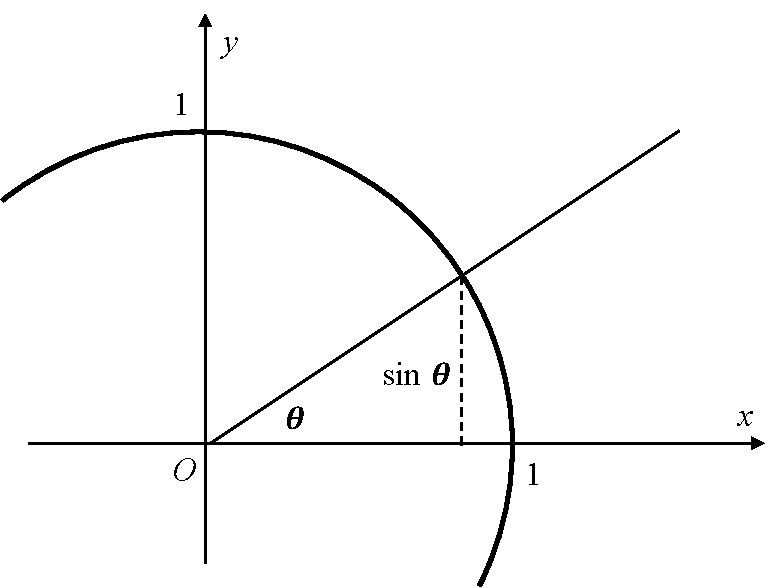
\includegraphics{./images/ch1/triFuncs.pdf}}
%   \end{center}
  \begin{figure}[!htb]
  	\centering
  	\resizebox{!}{3.5cm}{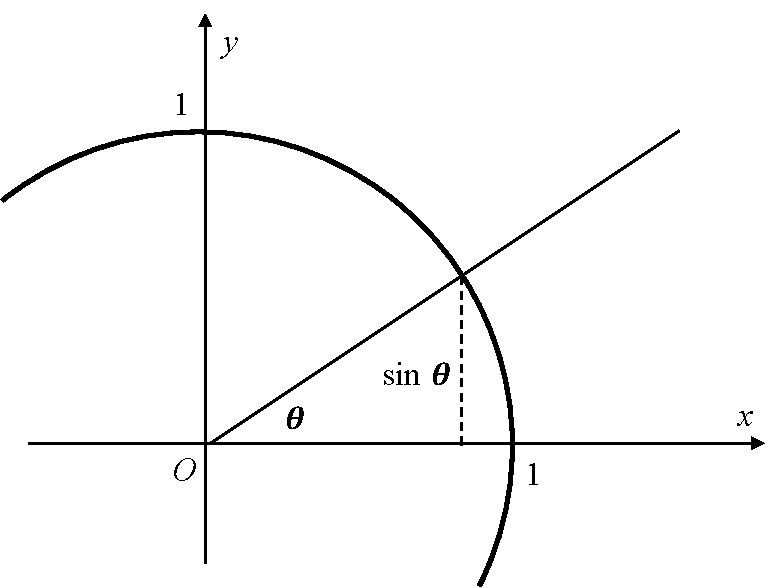
\includegraphics{./images/ch1/triFuncs.pdf}}
  \end{figure}
  \item 写出三角函数的{\it 和差化积}、{\it 积化和差}、{\it 半(倍)角公式}、{\it 万能公式}
  \item* 化简如下表达式:设$\theta\in\left(0,\pi/2\right)$
  \begin{enumerate}[(1)]
%     \setlength{\itemindent}{1cm}
    \item $\prod\limits_{i=1}^n\cos\df{\theta}{2^i}$
    \hspace{2cm}
    {\it(注:$\prod\limits_{i=1}^nf(i)=f(1)\cdot f(2)\cdot\cdots\cdot
    f(n)$)}
    \item $\sum\limits_{i=1}^n\cos i\theta$
  \end{enumerate}
  \item 证明以下等式与恒等式
  \begin{enumerate}[(1)]
    \item $\df{\pi}4=3\arctan\df14+\arctan\df5{99}$
    \item $3\arccos x-\arccos(3x-4x^3)=\pi,\;\left(|x|\leq\df12\right)$
    \item $2\arctan x+\arcsin\df{2x}{1+x^2}=\pi,\;(x>1)$
  \end{enumerate}
  \item 平面上任一点的位置可以既可以用直角坐标$(x,y)$表示,也可以用极坐标$(\rho,\theta)$
  表示,前者可用后者表示如下
  $$x(\rho,\theta)=\rho\cos\theta,\quad y(\rho,\theta)=\rho\sin\theta,$$
  反之,后者用前者应表示为(假设:$\rho\geq 0,\theta\in[0,2\pi]$)
  $$\rho(x,y)=\underline{\hspace{5cm}},\quad
  \theta(x,y)=\underline{\hspace{5cm}}.$$
  \item 比较以下函数值的大小,简述理由
  \begin{enumerate}[(1)]
    \item $x,\quad e^x-1,\quad \ln(x+1)$\quad$(x>0)$
    \item $\sin x,\quad \tan x, \quad \sec x, \quad x$ \quad $(x\in(0,\pi))$
  \end{enumerate}
  \item 证明函数$y=x+\sin x$在定义域内严格单调递增。({\it 注:函数$y=f(x)$严格单调
  递增,当且仅当对任意$x_1<x_2$,总有$f(x_1)<f(x_2)$})
  \item 本章习题中有如下定理:{\bf 任何一个定义在对称区间上的函数均可写成一个奇函数和一个
  偶函数的和},由此,
  $$e^x=\underline{\hspace{3cm}}_{\mbox{(奇)}}
  +\underline{\hspace{3cm}}_{\mbox{(偶)}}$$
  \item 写出下列集合之间的一一映射
  \begin{enumerate}[(1)]
    \item $(-1,1)\mapsto\mathbb{R}$\hspace{2cm}({\it 注:
  $\mathbb{R}=(-\infty,+\infty)$})
    \item $(0,+\infty)\mapsto\mathbb{R}$
    \item* $\{(x,y)\in\mathbb{R}^2|x^2+y^2<1\}\mapsto\mathbb{R}^2$
    \hspace{2cm}({\it 注:$\mathbb{R}^2$表示全平面)}
    \item 整数集$\mapsto$正整数集
    \item* 正整数集$\mapsto$正有理数集
  \end{enumerate}
  \item Fibnacci数列定义如下:$a_0=1$,$a_1=1$,
  $$a_{n+2}=a_{n+1}+a_{n},\quad n=1,2,\ldots,$$
  \begin{enumerate}[(1)]
    \item 请推导$\{a_n\}$的通项表达式;
    \item 设$p,q\in\mathbb{R}$,将前述递推式改为:
    $$a_{n+2}=p\cdot a_{n+1}+q\cdot a_{n},\quad n=1,2,\ldots,$$
    试讨论$\{a_n\}$通项表达式有何变化。
  \end{enumerate}
  \item* 写出不少于五位你听说过的数学家的名字(最好用英文),简述他们的事迹。
  \item 公理(Axiom)、假设(Assumption)、定理(Theorem)、定律(Law)有何异同?
  \item 以下函数中哪些是相同的,若不同,有何区别?
  $$x,\quad |x|,\quad e^{\ln x},\quad \ln(e^x),\quad \sqrt{x^2},\quad
	\frac{x^2-4}{x-2}-2,\quad
  \sin(\arcsin x),\quad \arcsin(\sin x), \quad \tan(\arctan x)$$
  \item 取整函数$[x]$的定义为{\it 不大于$x$的最大整数},请利用取整函数给出以下曲线的方程:
  \begin{center}
	\resizebox{!}{2.5cm}{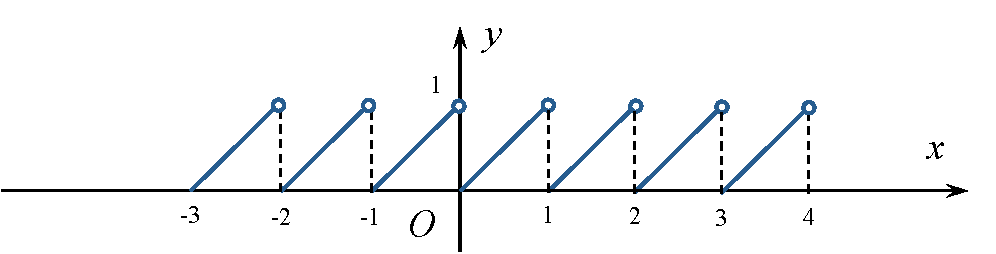
\includegraphics{./images/ch1/f1.pdf}}\\
	\resizebox{!}{2.5cm}{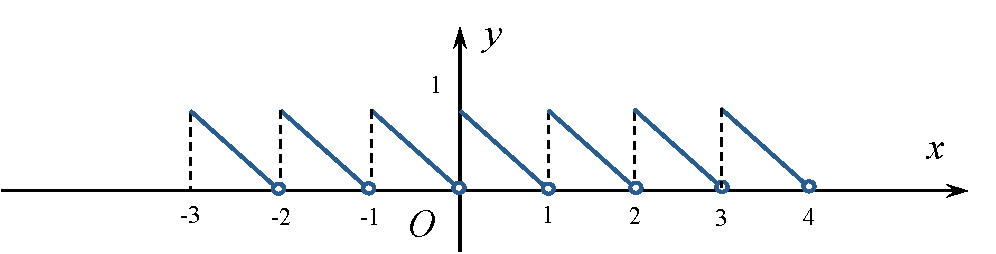
\includegraphics{./images/ch1/f2.pdf}}\\
	\resizebox{!}{2.5cm}{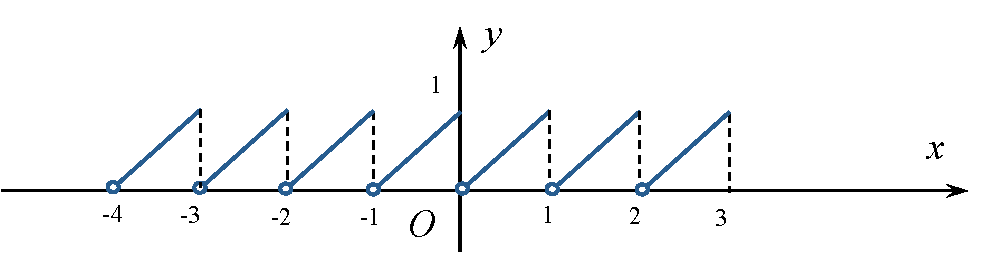
\includegraphics{./images/ch1/f3.pdf}}
  \end{center}
  \item 设$a\in\mathbb{R}$,且对任意$x\in\mathbb{R}$,有
  $f(2a-x)=f(x)$,
  请问$y=f(x)$的图像具有怎样的几何性质?若上式改为$f(2a-x)=-f(x)$,对应几何性质有何改变?
  \item 设$a\in\mathbb{R}$,且对任意$x\in\mathbb{R}$,有
  $f(a-x)=g(x)$,请问$y=f(x)$和$y=g(x)$的图像有何关系?
  \item 若对任意$x_1,x_2$,总有
  $[f(x_1)-f(x_2)](x_1-x_2)\leq 0$,
  由此可知函数$y=f(x)$具有何种性质?
  \item 给定集合$A\subset\mathbb{R}$,若$A$有界,是否必有最大和最小值?
  是否必有{\it 上确界}(最小的上界)和{\it 下确界}(最大的下界)?
  若$A$无界,是否必为无穷集合?
\end{enumerate}
% 
% \newpage

% \begin{center}
	{\bf\Large 格式说明}
\end{center}

\bigskip\bigskip

为了突出重点内容,区分不同要求,本讲义通过使用不同字体、色彩、背景
和文本框对内容加以区分,说明如下:

\bigskip\bigskip

宋体字:正文;

\bigskip\bigskip

{\kaishu 楷体字:}专有名词或概念;

\bigskip\bigskip

{\bf 黑体字}:重要概念或结论,各类标题;

\bigskip\bigskip

{\b 蓝色字体}:重要的附注或说明;

\bigskip\bigskip

{\color{red} 红色字体:}重要说明,务必重视;

\bigskip\bigskip

\begin{thx}
	深蓝色边框,白色底色文本框:重要概念或结论;
\end{thx}

\bigskip\bigskip

\begin{ext}
	深绿色边框,绿色底色文本框:课后作业或练习题;
\end{ext}

\bigskip\bigskip

\begin{shaded}
	黑色背景文本框:扩展阅读知识,了解即可,不要求掌握;
\end{shaded}

\bigskip\bigskip

边栏文本:\ps{附注和说明。}

\newpage

\section{课程简介}

\subsection{学什么}

高等数学是大学工科专业必修的数学基础课,通常和{\it 线性代数}、{\it 概率论与数理统计}统称
为{\it 工程数学}。

我们所说的高等数学,在国外一般就叫做{\it 微积分},而且通常分为{\it 一元函数微积分}
和{\it 多元(高维)微积分}两个部分。而国外所说的{\it 高等数学}就是我们说的工程数学。

我们一般认为,微积分诞生于17世纪中叶,当时的两位数学巨匠Newton(1642-1726)和
Leibniz(1646-1716)分别独立
创立了微积分的理论,并最终被视为微积分的共同创始人。但是,我们必须认识到的是,
一门系统、复杂的理论,不可能仅仅是极个别人的创造。正如Newton的名言,“{\it If 
I have seen further, it is by standing on the shoulders of
giants.}”,在两位大师生前和生后,众多杰出的数学家都为微积分理论的发展作出了
贡献,其中既包括Fermat(1607-1665)、Barrow(1630-1677)、
Descartes(1596-1650)%、Huygens(1629-1695)、Wallis(1616-1703)
等人的奠基性工作,也包括Cauchy(1789-1857)、D.Bernoulli(1700-1782)、
Lagrange(1736-1913)、Weierstrass(1815-1897)、Cantor(1845-1918)、
Taylor(1685-1731)、Euler(1707-1783)、d'Alembert(1717-1783)
%、Laplace(1749-1827)、Agnesi(1718-1799)
使之严谨化以和完善,更包括Dirichlet(1805-1859)、Riemann(1826-1866)、
Lebesgue(1875-1941)、Fourier(1772-1837)以及后世很多数学家在{\it 分析
学}上的深入探索。今天我们所学习的微积分,虽然只是这一学科
\ps{更准确的说法应该叫分析学,它和几何学、代数学并称现代数学的三大分支,
三者各自拥有庞大的理论体系,在它们的交汇处诞生了众多重要而又生机勃勃的
数学前沿分支}的基础部分,但要说其中融汇了300多年来众多近现代数学家
的杰出成就,是绝对实至名归的。

% \begin{figure}[htbp]
% 	\centering\scalebox{0.3}{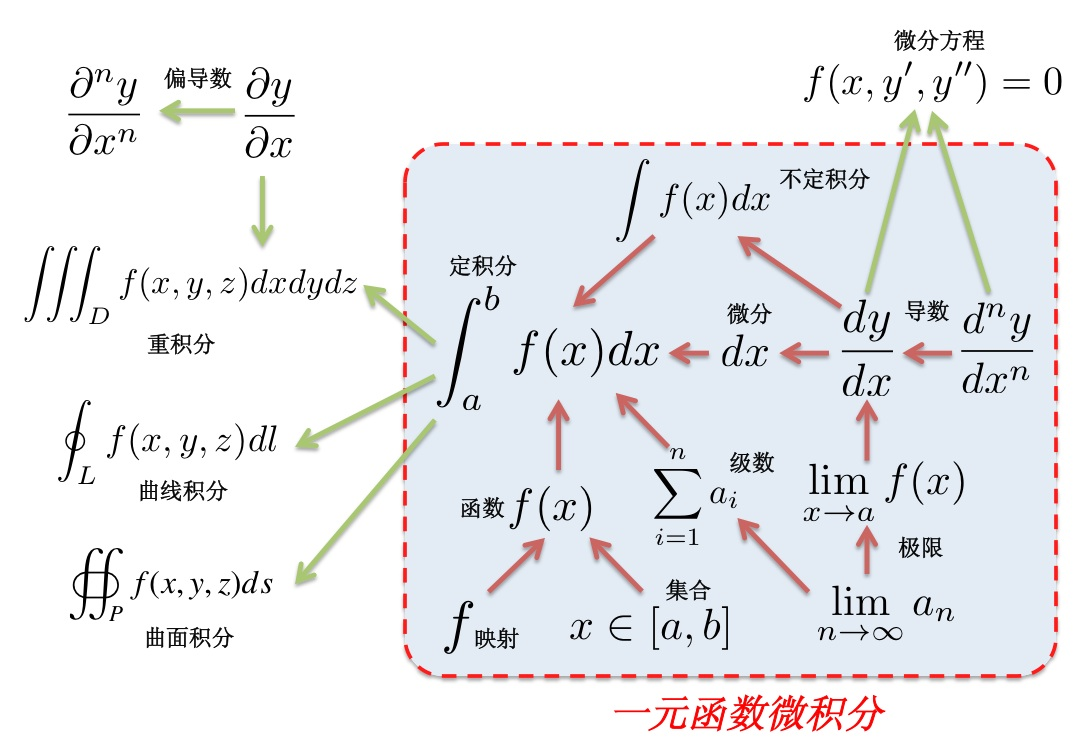
\includegraphics{./images/ch1/AM_architecture.jpg}}
% 	\caption{微积分中的主要概念及其关系\;
% 	({\it 个人整理,仅供参考})}
% % 	\label{图:0.1}
% \end{figure}

% \begin{center}
% 	\scalebox{0.3}{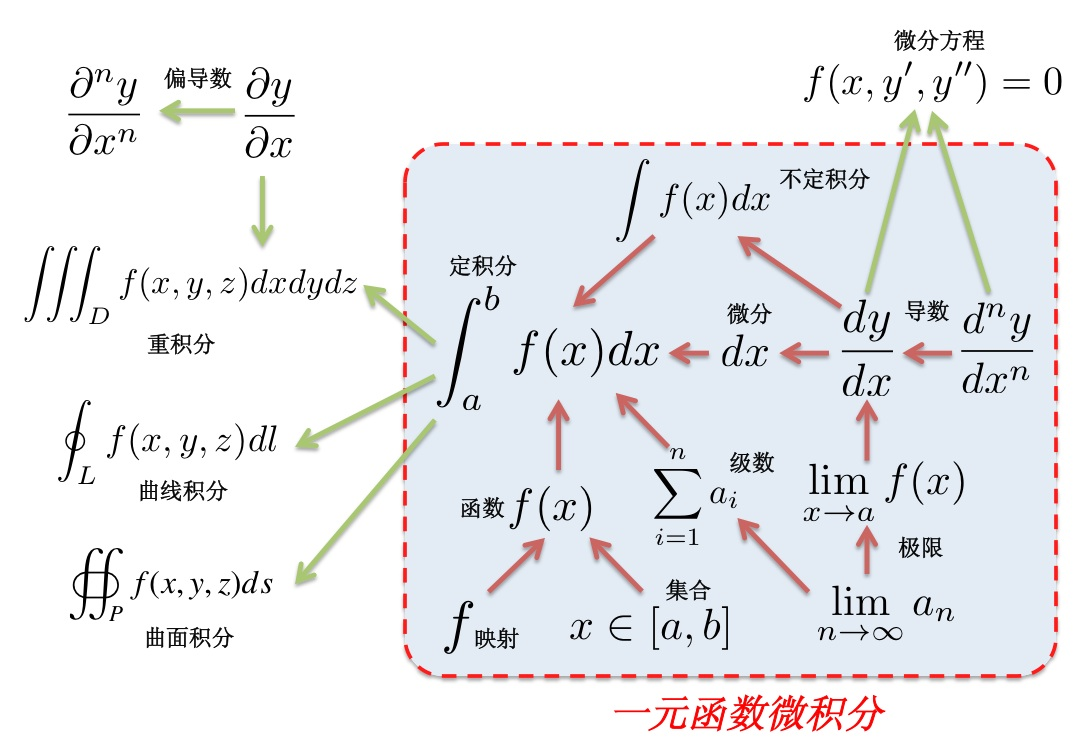
\includegraphics{./images/ch1/AM_architecture.jpg}}
% % 	\ps{上课前画好}
% \end{center}

\begin{center}
	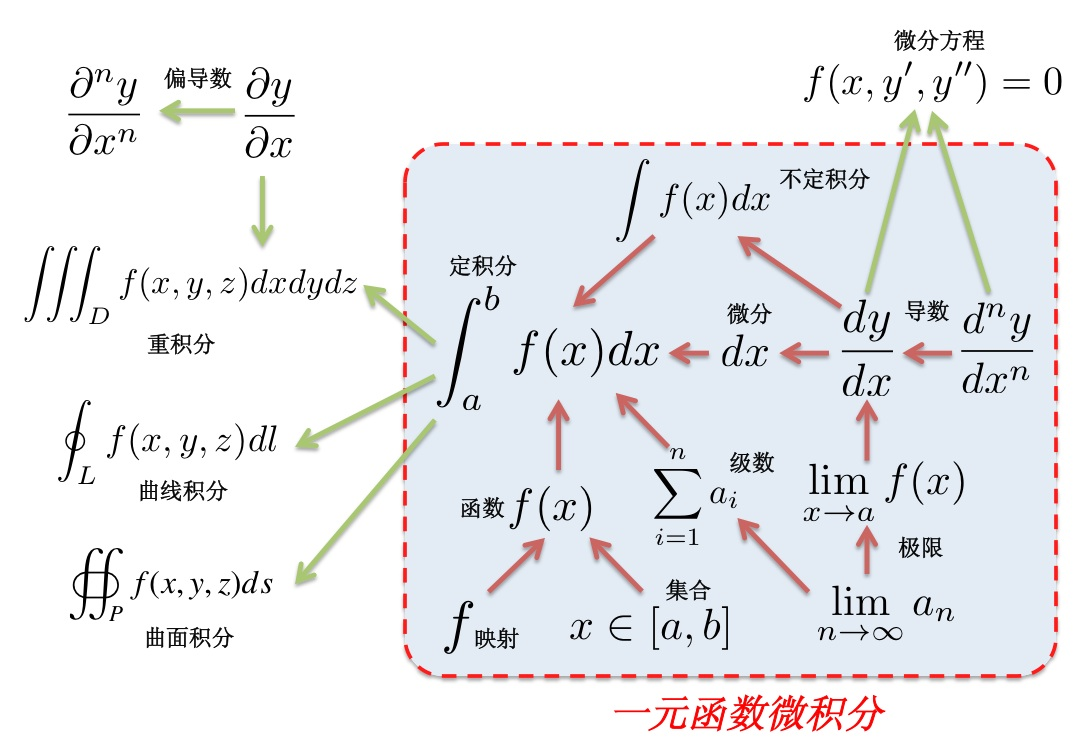
\includegraphics[width=0.8\textwidth]{./images/ch1/AM_architecture.jpg}
	
	{微积分中的主要概念及其关系\;
	({\it 个人整理,仅供参考})}
\end{center}

\begin{itemize}
	  \item {\bf Wikipedia——微积分(Calculus)} 
	\begin{itemize}
	  \item Latin: {\it a small stone used for counting}  
	  \item {\it a branch of mathematics focused on \underline{limits, functions,
	  	derivatives, integrals, and infinite series}} 
  	  \item {\it widespread application in \underline{science, economics,} 
  	  and \underline{engineering}} 
	  \item {\it constitues a major part of modern mathematics}
	  \item {\it 微}的意思是很小的东西,如微生物,{\it 积}就是加起来的意思,
	  {\it 积分}的意思就是把极小的东西加起来。微,是积的相反。 
	\end{itemize}
	\item {\bf John von Neumann} ({\small\it The Mathematician, 1947})
	\begin{itemize}
	  \item {\it The calculus was the \underline{first achievement} of modern
	  mathematics, and it is difficult to overestimate its importance.}
	\end{itemize} 
\end{itemize}

\subsection{为什么学}

微积分为什么如此重要,毫无疑问,与其在众多领域的应用密不可分,甚至可以说,
在其中绝大多数的问题中,微积分的作用是无可替代的。任何一门工科类的专业课程,
只要涉及与连续运动(变化)相关的问题,都不可避免地会以微积分作为其预备知识,
或者说,将这些课程视为微积分的应用也不为过。

当然,微积分不总是“美丽”的,因为它的美可能不是那么显而易见。我们很难用一两句话
来描述,微积分到底有什么用?它美在哪里?但是,一旦你理解了微积分背后的深刻思想,
开始能够将其应用于解决一些实际问题,或者通过它理解一些最前沿的科技成就时,
你一定会对它的美产生深深地赞叹,也许那时,再回头来看微积分的重要性也就不言而喻了。

学习微积分的过程也许会有些枯燥甚至痛苦\ps{“从前有棵树,叫高数,上面挂了很多人”}
,但它无疑是值得的,能够从看似单调痛苦的过程中领略数学的美丽,发现它的深刻与强大,
也是它作为“{\it 大学第一课}”\ps{无论从体量、难度还是学习的先后来看}所期望带给
大家的体验。

\begin{shaded}
	{\bf 知乎:学数学有什么好处?我们为什么要学数学?}
	\begin{itemize}
	  \item Engles:{\it 数学是一门研究现实世界的数量关系和空间形式的科学。}数学具有:
	  抽象性、精确性和应用的广泛性
	  \item Marx:{\it 一种科学只有在成功运用数学时,才算达到了真正完善的地步。}
	  \item Galileo:{\it “数学符号就是上帝用来书写自然这一伟大著作的统一语言,
	  不了解这些文字就不可能懂得自然的统一语言,只有用数学概念和公式所表达的物理世界
	  的性质才可认识……”}
	  \item Gauss:{数学是科学的女王}
	  \item 韩寒:{\it
	  我们生活中用到的数学估计到小学三年级就已经够用了。}然而在之后我们多年来学习的数学,
	  实际上塑造了我们一种理性的、条理的、系统化的思维方式。这种思维方式在我们解决自己
	  一生中遇到的诸多问题时,都有非常重要的作用。比如慎密的思考、分类的思想、排序的思想等。
	  很多东西其实都带有学习数学这个过程产生的影响,只是由于其作用方式非常隐晦,
	  也不容易被追溯其源头,我们平时不容易注意到罢了。
	  \item 王小波:{\it 我上大学时,有一次我的数学教授在课堂上讲到:我现在所教的数学,
	  你们也许一声都用不到,但我还要教,因为这些知识是好的,应该让你们知道。”}
	  \item 崔钢:{\it\b 1,用通用简洁的方式来表达自然规律。2,提供一些问题的分析手段。
	  3,提供认识世界的一种模式。4,了解自己的智力水平。.}
	\end{itemize}
	{\bf 豆瓣:为什么没人喜欢学习高等数学?木遥}
	\begin{itemize}
% 	  \item {\it 我完全不能理解,一个非数学或物理专业的学生怎么可能从这样的教育中获得一丝一毫的教益?
% 	  他怎么可能不发自内心地痛恨这门课程,然后在考完试之后的一个小时之内把所有内容忘得精光?
% 	  象三角代换这类积分技巧,不要说一个普通的心理学或者经济学专业的学生一辈子都用不到,
% 	  就连我也一辈子都用不到。就算在极其罕见的情形下需要求解这类问题,也完全可以求助于
% 	  wolframalpha.com 或者类似的工具。
	  \item 在我看来,在二十一世纪还要求一个普通学生手算积分,
	  就像是要求一个汽车驾校学员一定要从骑马学起一样。
	  \item \ldots 一本基于数学家思维方式写出来的教材,亦即在每一个课题上从最基本的定义
	  和定理开始堆砌,直到超出教材所可能涵盖的水平为止
	  \item 如果是我来编写大学数学教材,我会争取让每一个在大学里读过数学课的人都能回答这样的问题:
	  为什么人们能精确预测几十年后的日食,却没法精确预测明天的天气;为什么人们可以通过 https 
	  安全地浏览网页而不会被监听;为什么全球变暖的速度超过一个界限就变得不可逆了;
	  为什么把文本文件压缩成 zip 体积会减少很多,而 mp3 文件压缩成 zip 大小却几乎不变;
	  民生统计指标到底应该采用平均数还是中位数;当人们说两种乐器声音的音高相同而音色不同的时候
	  到底是什么意思\ldots\ldots这不是什么「趣味数学」,这就是数学。基础、重要、深刻、美的数学。
	  \item 在我的设想里,这才是大学基础数学教育所应该达成的任务。
	  {\it 不是培养一个非数学专业的现代人在数学领域的专业素质(这是无论如何也不可能成功的),
	  而是让一个人能够在非专业的前提下最大程度地掌握真正有用的现代数学知识,
	  了解数学家们的工作怎样在各个层面上和社会产生互动,以及社会在这个领域的投资得到了怎样的回报。}
	  别的科学门类的基础教育也应当是这样。
	\end{itemize}
	{\bf 知乎:学习编程及做程序员对微积分的要求高吗?}
\end{shaded}

\begin{itemize}
  \item {\bf 数学的三大功能}
  \begin{enumerate}
    \item 为学习其他知识(课程)提供数学工具
    \item 培养理性思维
    \item 弘扬数学文化
  \end{enumerate}
  \item {\bf 数学素质}
  \begin{enumerate}
    \item 从实际问题抽象出数学模型的能力
    \item 计算与分析的能力
    \item 了解和使用现代数学语言和符号的能力
    \item 使用数学软件学习和应用数学的能力
  \end{enumerate}
\end{itemize}

\subsection{怎么学}

\begin{itemize}
	\item {\bf 参考资料}
  	\begin{enumerate}
		\item {\bf 课程配套辅导}
	  	\begin{itemize}
	  	  \item \underline{同济大学数学系,高等数学(第七版,上、下),高等教育出版社,2014,北京}
	  	  	\ps{简称:\b 同济}  
	  	  \item 朱健民 等,高等数学(第二版,上、下),高等教育出版社,2015,北京
	  	  	\ps{简称:\b KD教材} 
	      \item 李建平 等,高等数学典型例题与解法(上、下),国防科技大学出版社,2009,长沙
	    	\ps{简称:\b 辅导书} 
	  	\end{itemize}
  		\item {\bf 参考书} 
  		\begin{itemize}
	    	\item 菲赫金哥尔茨,微积分学教程(第一至三卷),第8版,高等教育出版社,2006,北京
	    	  \dotfill{\it\b 读不懂不必勉强,它回答不了的微积分问题大学阶段你肯定碰不到} 
	    	\item James Stewart, Calculus(11th eds.)(影印版,上、下册),高等教育出版社,2016,北京
	    	  \dotfill{\it\b 大部头,但绝对浅显易懂}
	    	\item 斯蒂芬.弗莱彻.休森,数学桥,上海科技出版社,2010,上海
	    	  \ldots\dotfill{\it\b 值得常常拿出来读的数学书,一遍绝对不够} 
	    	\item William Dunham,微积分的历程——从牛顿到勒贝格,人民邮电出版社,2011,北京
	    	\dotfill{\it\b 了解微积分的历史,能够更好地理解其中深刻的思想} 
  		\end{itemize}
  		\item {\bf 在线资源}
  		\begin{itemize}
  		  \item 朱健民,高等数学(一-五),中国大学MOOC%,http://www.icourse163.org/course/NUDT-9004
  		    \ps{简称:\b MOOC}\ldots
  		    \dotfill{\it\b 缺课或者课上没听懂,就用它补补课}
  		  \item 李建平\,等,高等数学典型例题与解法(一、二),中国大学MOOC%,\\
  		    %http://www.icourse163.org/course/NUDT-1001979006
  		    \ldots\dotfill{\kaishu\b 辅导书的配套MOOC}
  		  \item 闫浩,高等数学习题课,学堂在线%,\\
  		     %https://xuetangx.com/courses/course-v1:BUPT+3412113011+2017_T2/about
  		     \dotfill{\it\b 讲得棒极了,这老师其实是清华的}
%   		  \item 李建平\,等,微积分CAP,中国大学MOOC%,
  		     %http://www.icourse163.org/course/NUDT-1001626005
%   		    \dotfill{\it\b 高中没学好,来这补一补}
		\end{itemize} 
		\item {\bf 扩展阅读}\dotfill{\it\b 读一些课外书,让学习显得不那么枯燥}
		\begin{itemize}
		  \item 基斯.德夫林,数学思维导论,人民邮电出版社,2016,北京
		  \item G.波利亚,怎样解题:数学思维的新方法,上海科技教育出版社,2011,上海
		  \item 李学数,数学与数学家的故事(1-5),上海科学技术出版社,2015,上海
		  \item 塞德里克·维拉尼\,等,一个定理的诞生:我与菲尔茨奖的一千个日夜,人民邮电出版社,2016,北京
		  \item 春日真人,庞家莱猜想:追寻宇宙的形状,人民邮电出版社,2015,北京
		  \item 蒂莫西.高尔斯,数学,译林出版社,2014,南京
		  \item 吴军,数学之美,人民邮电出版社,2016,北京
		  \item 李建平,漫谈数学与军事,中国大学MOOC
		  \item \ldots\ldots
		\end{itemize}
	\end{enumerate}
	\item {\bf 学习方法}
% 	\begin{itemize}
% 	  		\item {\bf 听课}\dotfill {\bf 30}
% 		\begin{itemize}
% 	  		  \item 典型问题、典型方法
% 	    	  \item 师傅领进门,修行在个人
% 	 	\end{itemize}
% 	  		\item {\bf 练习}\dotfill {\bf 50}
% 	 	\begin{itemize}
% 	    		\item 熟能生巧!
% 	    		\item 记忆!琢磨!
% 	  	\end{itemize}
% 	  		\item {\bf 思考}\dotfill {\bf 20}
% 	  	\begin{itemize}
% 	    		\item 总结!
% 	    		\item 质疑!
% 	  	\end{itemize}
% 	\end{itemize}
	\begin{enumerate}
	  \item {\bf 预习:}课前3-5分钟,快速翻阅教材,浏览本讲内容梗概,
	  标记出新的名词和例题,试着理解其大概意思,确保听课时心中有数;
	  \item {\bf 听课:}抓住关键思路,卡住了或者有疑点立即举手问,
	  简要记笔记\ps{推荐:\b 康奈尔笔记法},重点记思路和书本上没有的内容
	  \item {\bf 复习:}要么读教材,要么读笔记,也可以先作习题,搞不定
	  再回来翻书查笔记,重在理清思路\ps{重要概念,典型问题,典型方法},
	  消化细节,肯花时间才有好的效果
	  \item {\bf 练习:}作业之外,有选择地作题,学习也是个熟能生巧的过程,
	  提高效率是关键\\
	  G.Polya:{\it 我们的任何一门学问都由知识和技能组成。如果你对初等或高等数学的研究工作
	  的确有真正的经验的话,那么你对下述这一点将毫不怀疑:在数学中,技能比仅仅掌握
	  一些知识要重要得多。什么是技能呢?数学技能就是解题能力——不仅能解决一般的问题,
	  而且能解决需要某种程度的独立思考、判断力、独创性和想象力的问题}
	  \item {\bf 思考:}多琢磨,让知识点在大脑中结成网络,融会贯通,
	  会提问是思考能力的体现\ps{Einstein:提出一个问题往往比解决一个问题更重要!}
	  \centerline{\it What$\to$How$\to$Why$\to$Why not$\to$What if}
	\end{enumerate}
\end{itemize}

\section{几点要求}
\begin{itemize}
	\item {\bf 课堂:安静!安静!!安静!!!}
	尊重他人学习的权利,安排好自己的时间
	
	{\bf - No to}
	  \begin{itemize}
	    \item Chatting
	    \item zZZ\ldots
	    \item anything noisy
	    \item \ldots
	  \end{itemize}
	{\bf - Yes to}
  \begin{itemize}
    \item listen to me
    \item discuss {\bf with me}
    \item do sth. you like {\bf quietly}
    \item zzz\ldots
    \item leave/enter the classroom {\bf quietly}
    \item \ldots
  \end{itemize}
  \item {\bf 作业}
  \begin{center}
  	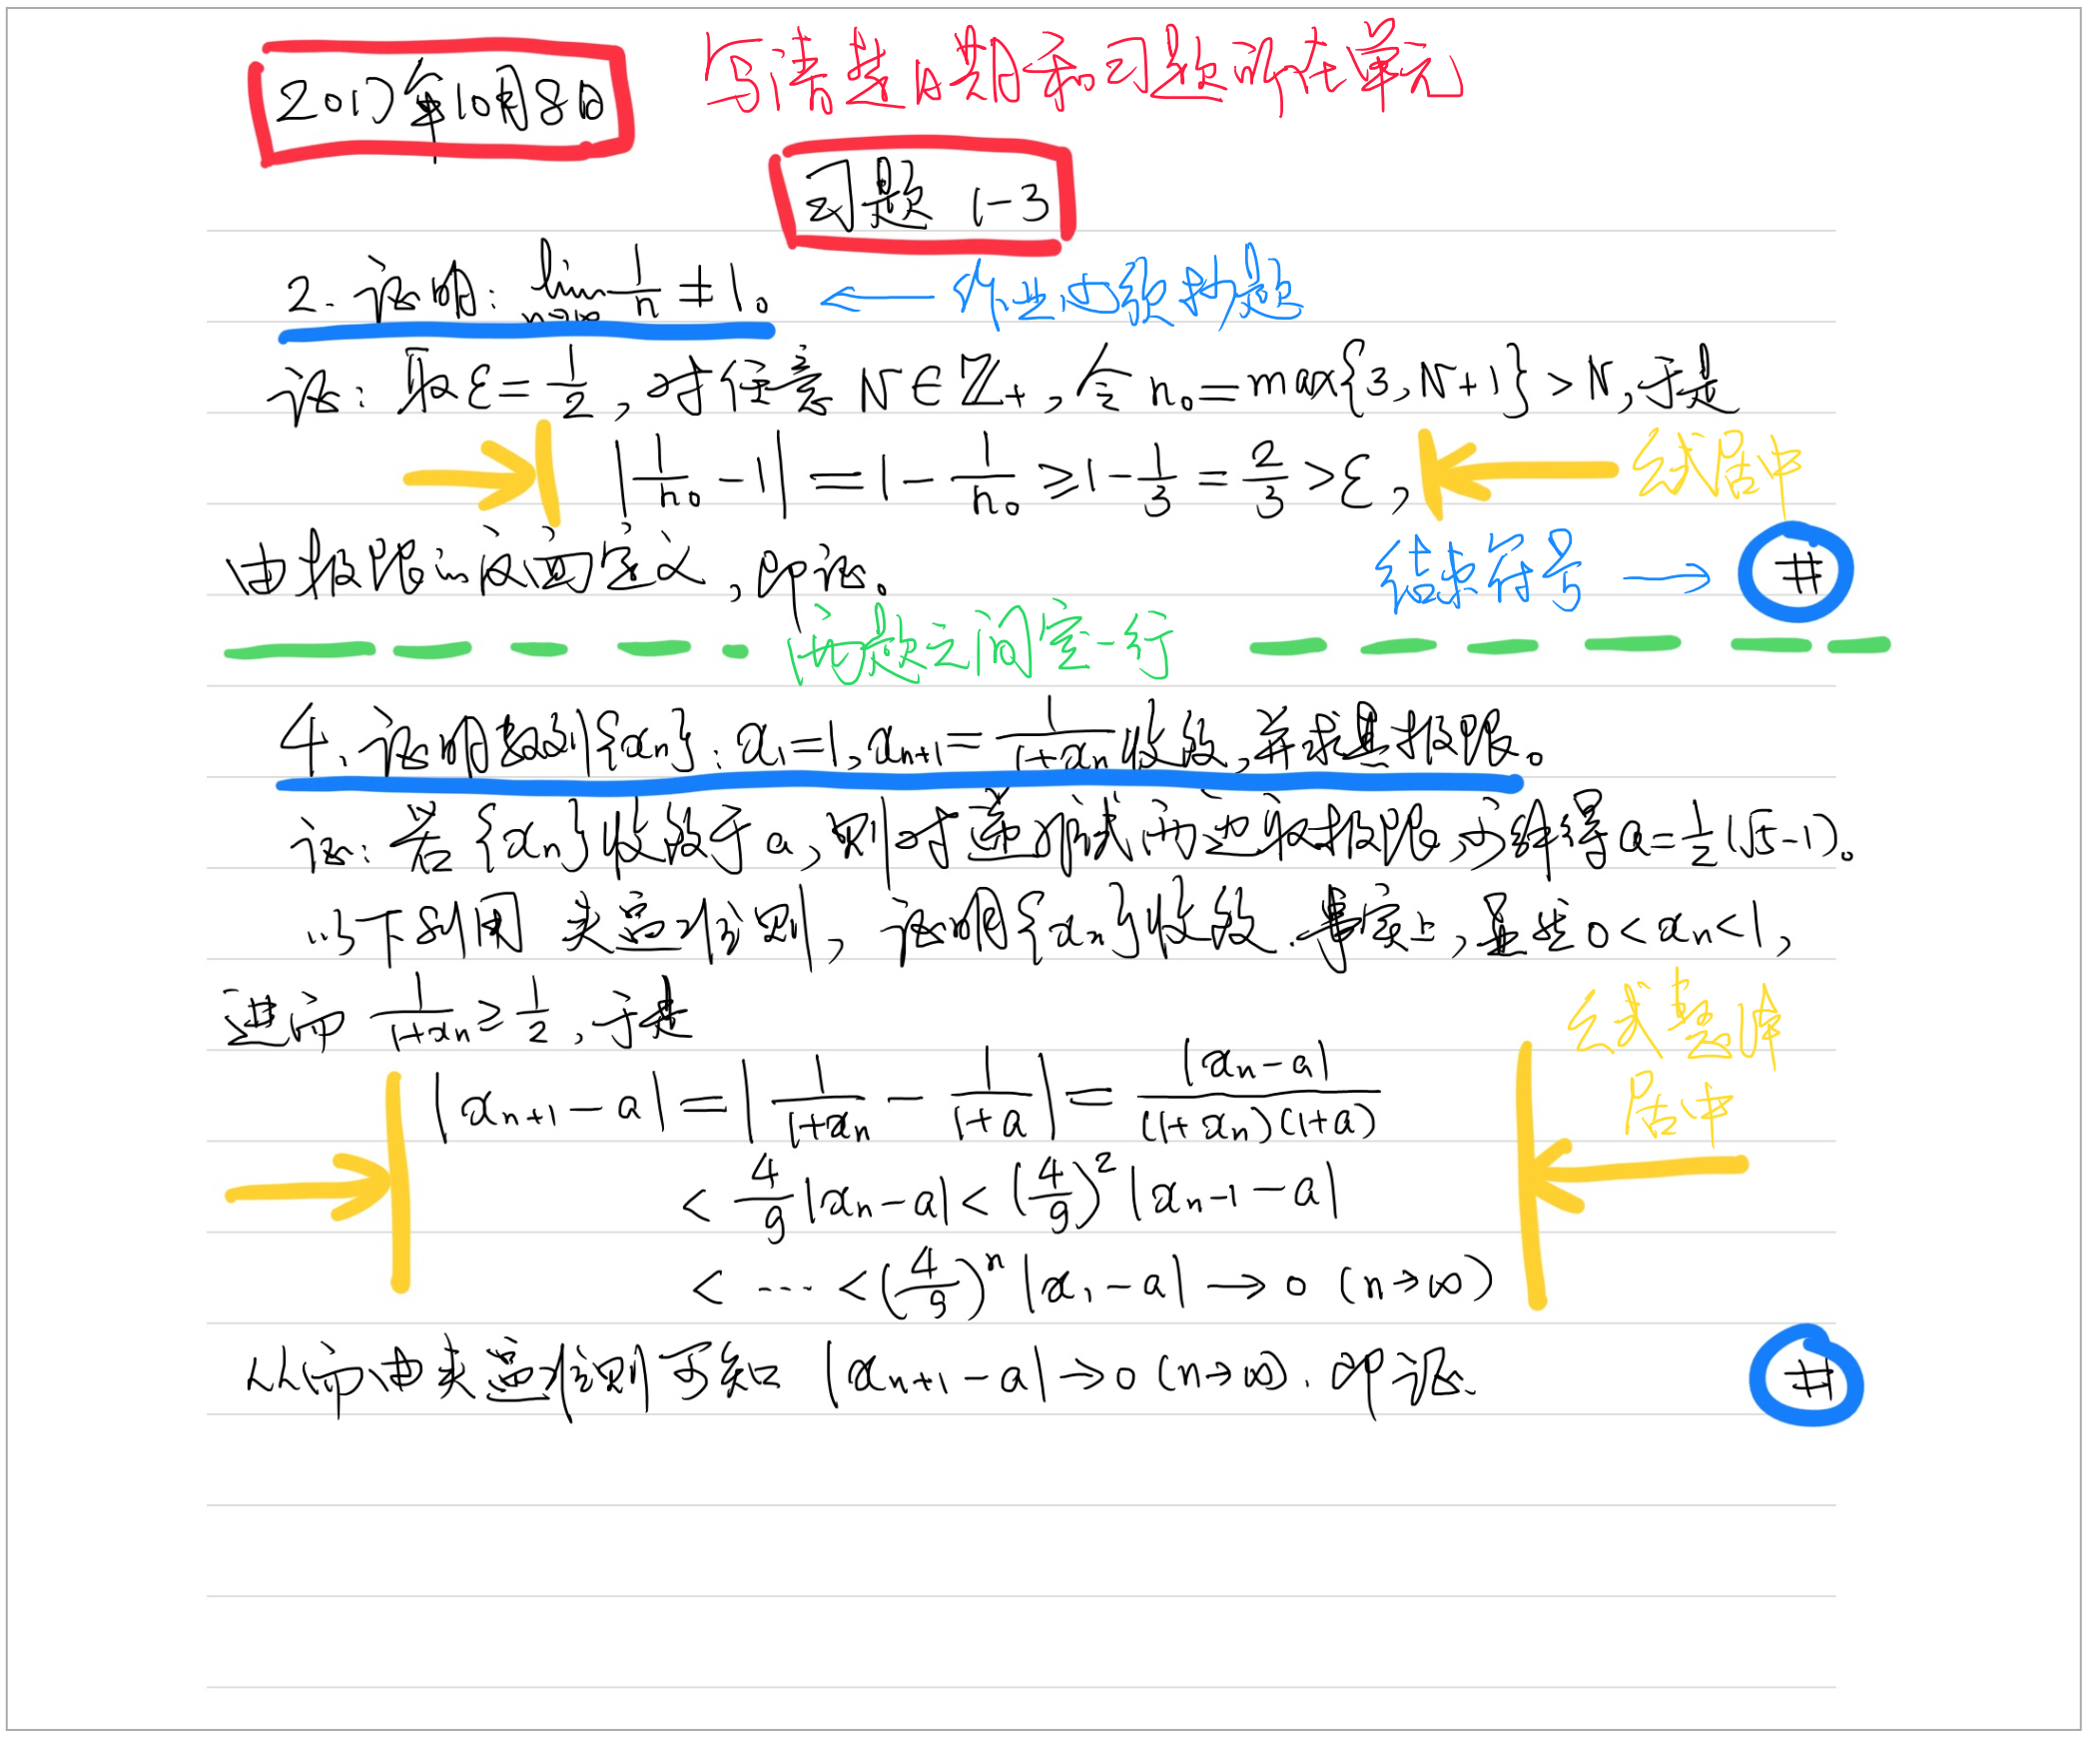
\includegraphics[width=0.95\textwidth]{./images/00/hw-sample.jpg}
  	
  	作业书写参考样式({\it 以黑色字体为准,彩色部分为格式说明})
  \end{center}
  \begin{itemize}
    \item 作业书写的规范
    \begin{enumerate}
      \item 写清楚作业日期(对应讲课的日期)和习题所在单元;
      \item 作业必须抄题,写清楚题号
	  \item 解题过程以“证:”或“解:”开始,以$\#$号结束;
	  \item 公式整体居中书写;
	  \item 无论大题小题,两题之间空一行;
	  \item 不允许使用铅笔、红笔书写作业,可以用铅笔画图;
	  \item 作业本不许分栏使用;
	  \item 文字、符号书写清晰规范,尽量少涂改。
    \end{enumerate}    
    \item no copy ??!
    \item 及时订正错误,补上缺漏
  \end{itemize}
	\item {\bf 答疑}
	  \begin{itemize}
	    \item 每周一次面对面答疑,1-2小时
	    \item 提问题的能力不完全是天生的,脸皮要厚一点
	    \item 综合利用各种手段(微信、网站、邮件、\ldots)
	  \end{itemize}
% 	  \item {\bf 从善如流}
\end{itemize}

\section{关于考试}

以下是2017-2018学年开始实施的“{\it 新政}”:

考试分为{\it 形成性考试}和{\it 终结性考试}两个部分,两部分成绩按照$40\%$和$60\%$的比例综合
得到最终的课程期末成绩。

每学期末设一次终结性考试,采用闭卷笔试形式。{\color{red}\bf 终结性考试不及格,
则课程成绩不合格!}

每学期的形成性考试分为四个部分,一是{\it 平时作业和表现}成绩,占$10\%$,剩下的为三次
{\it 单元测试}成绩,各占$10\%$。

单元测验的形式为笔试或网络测试,具体待定。

\bigskip

\begin{ext}
	{\centering\bf 课后作业}
	
	{\b\it 说明:作业必须写明题目所在章节、页码、题号;如非特别说明,
	所有题目必须抄题;两道题之间空一行;未作或作错的题目讲评后务必及时订正。}
	
	\begin{itemize}
	  \item 注册加入课程网站:https://www.trustie.net/courses/1259,邀请码:YRKWF
	  \item 注册中学大学MOOC账号:http://www.icourses.cn/imooc/,将用户名告知课代表
	  统一登记
	  
	  {\b\it 下面的题目请写在活页纸上,不用抄题:}
	  \item 写一篇短文,内容及要求如下
	  \begin{enumerate}[(1)]
	    \item 你的个人介绍,请务必包含如下信息:姓名、性别、年龄、籍贯、中学母校的名字、
	    你的高考总成绩(以及当地的满分)、你的高考数学成绩(以及当地的满分);
	    \item 你的兴趣爱好、特长,或者说,你觉得自己有什么与众不同之处;
	    \item 你学习数学的体会,例如:喜欢,不喜欢?喜欢什么样的数学,不喜欢什么样的数学?
	    有什么好的学习方法?有什么自己觉得成功的经验,或者有趣的经历(最好与数学有关)?
	    \item 你期待中的大学课堂是怎样的?怎么的教与学会对你更有帮助?对老师有什么期待、要求,
	    或者建议?
	    \item 请至少推荐一本(部、套)你喜欢的书、电影或者其他任何可以通过公共渠道获取到的资料
	    (例如:网站、软件、APP、\ldots),说说推荐的理由;
	    \item 其他任何你认为值得(可以)与我交流的东西,比如你想问我什么问题;
	    \item 除第一条必须包含外,其余内容可自由取舍。
	    \item 篇幅:不少于半页,不多于两页(一张纸的正反面)。
	  \end{enumerate}
% 	  {\b\it 以下的题目写在作业本上,作业本第一页背面上贴上一张个人的照片,标注专业和籍贯}
% 	  \item 习题1-2:5(3,4),7,8
% 	  \item 习题1-3:5(3),6(2),7,8
% 	  \item 习题1-4:7,8
% 	  \item 习题1-5:3
% 	  \item 习题1-6:4(2,3,5)
% 	  \item 习题1-7:4(2),5(3,4)
% 	  \item 习题1-8:4
% 	  \item 习题1-9:2,3(3,5,6),4
% 	  \item 习题1-10:1,5,7
% 	  \item 总习题一:14
	\end{itemize}
\end{ext}

\newpage

\begin{shaded}
	{\bf\Large Cornell Note-Taking System}\hfill{\it 康奈尔笔记法(5R笔记法)}
	
	\bigskip
	
	这一方法适用于一切依赖讲授或自学的学习过程,特别是对于听课笔记,5R笔记法堪称首选。
	该方法的重点是记与学、思考与运用的结合,以及将笔记的记录与完善作为学习的过程载体。
	最终完成的笔记类似于下图:
	
% 	\begin{figure}[htbp]
% 		\centering
% 		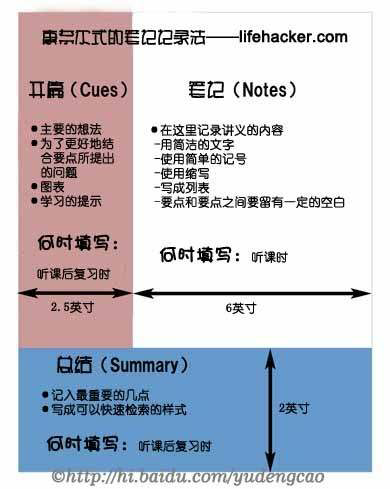
\includegraphics[width=0.4\textwidth]{./images/00/Cornell-NTS/NTS-CH.jpg}\quad
%  		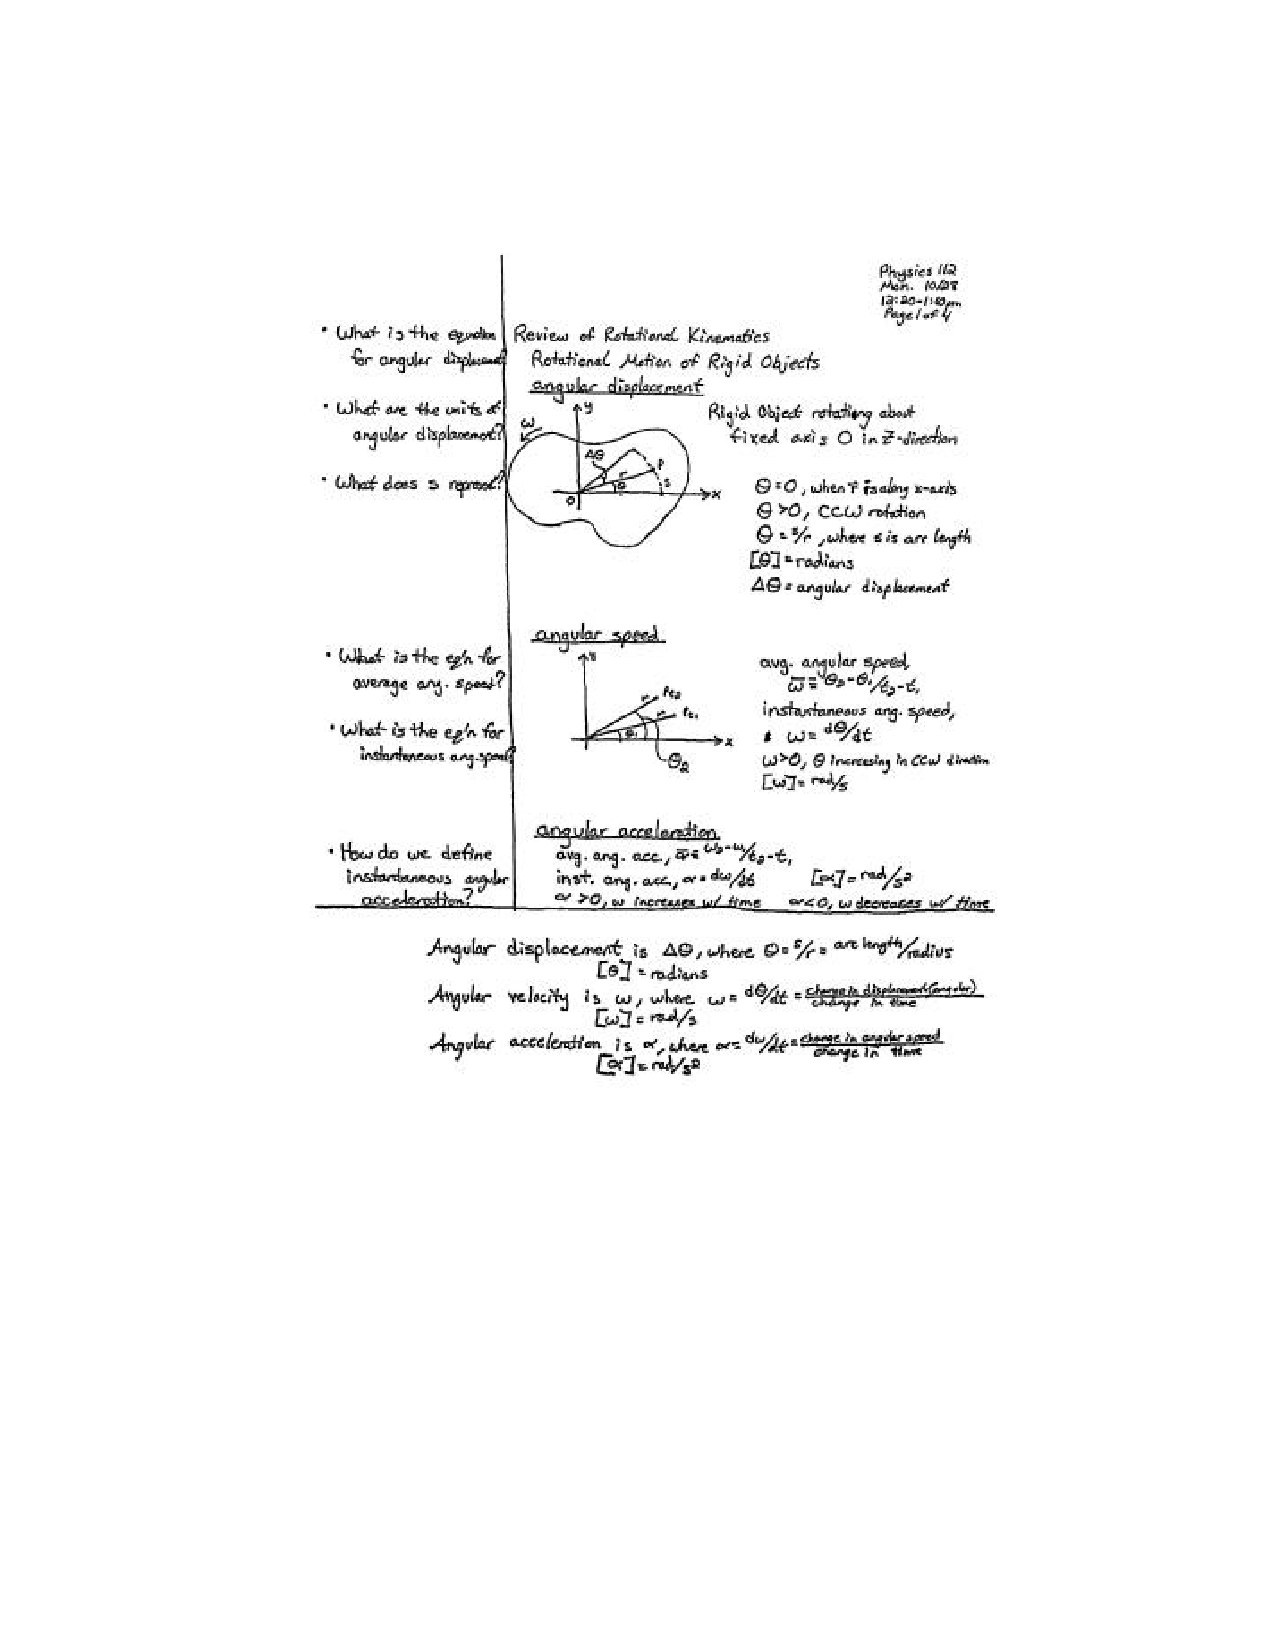
\includegraphics[height=8cm]{./images/00/Cornell-NTS/exCNTS.pdf}
% 	\end{figure}
	
	\begin{center}
		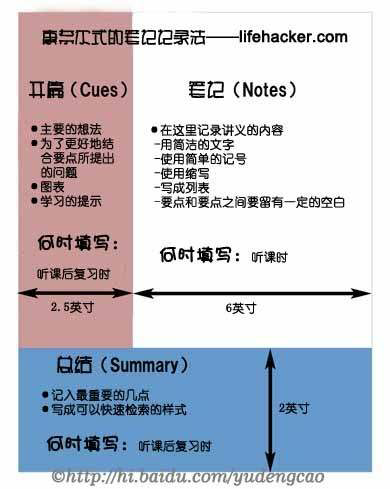
\includegraphics[height=8cm]{./images/00/Cornell-NTS/NTS-CH.jpg}\quad
		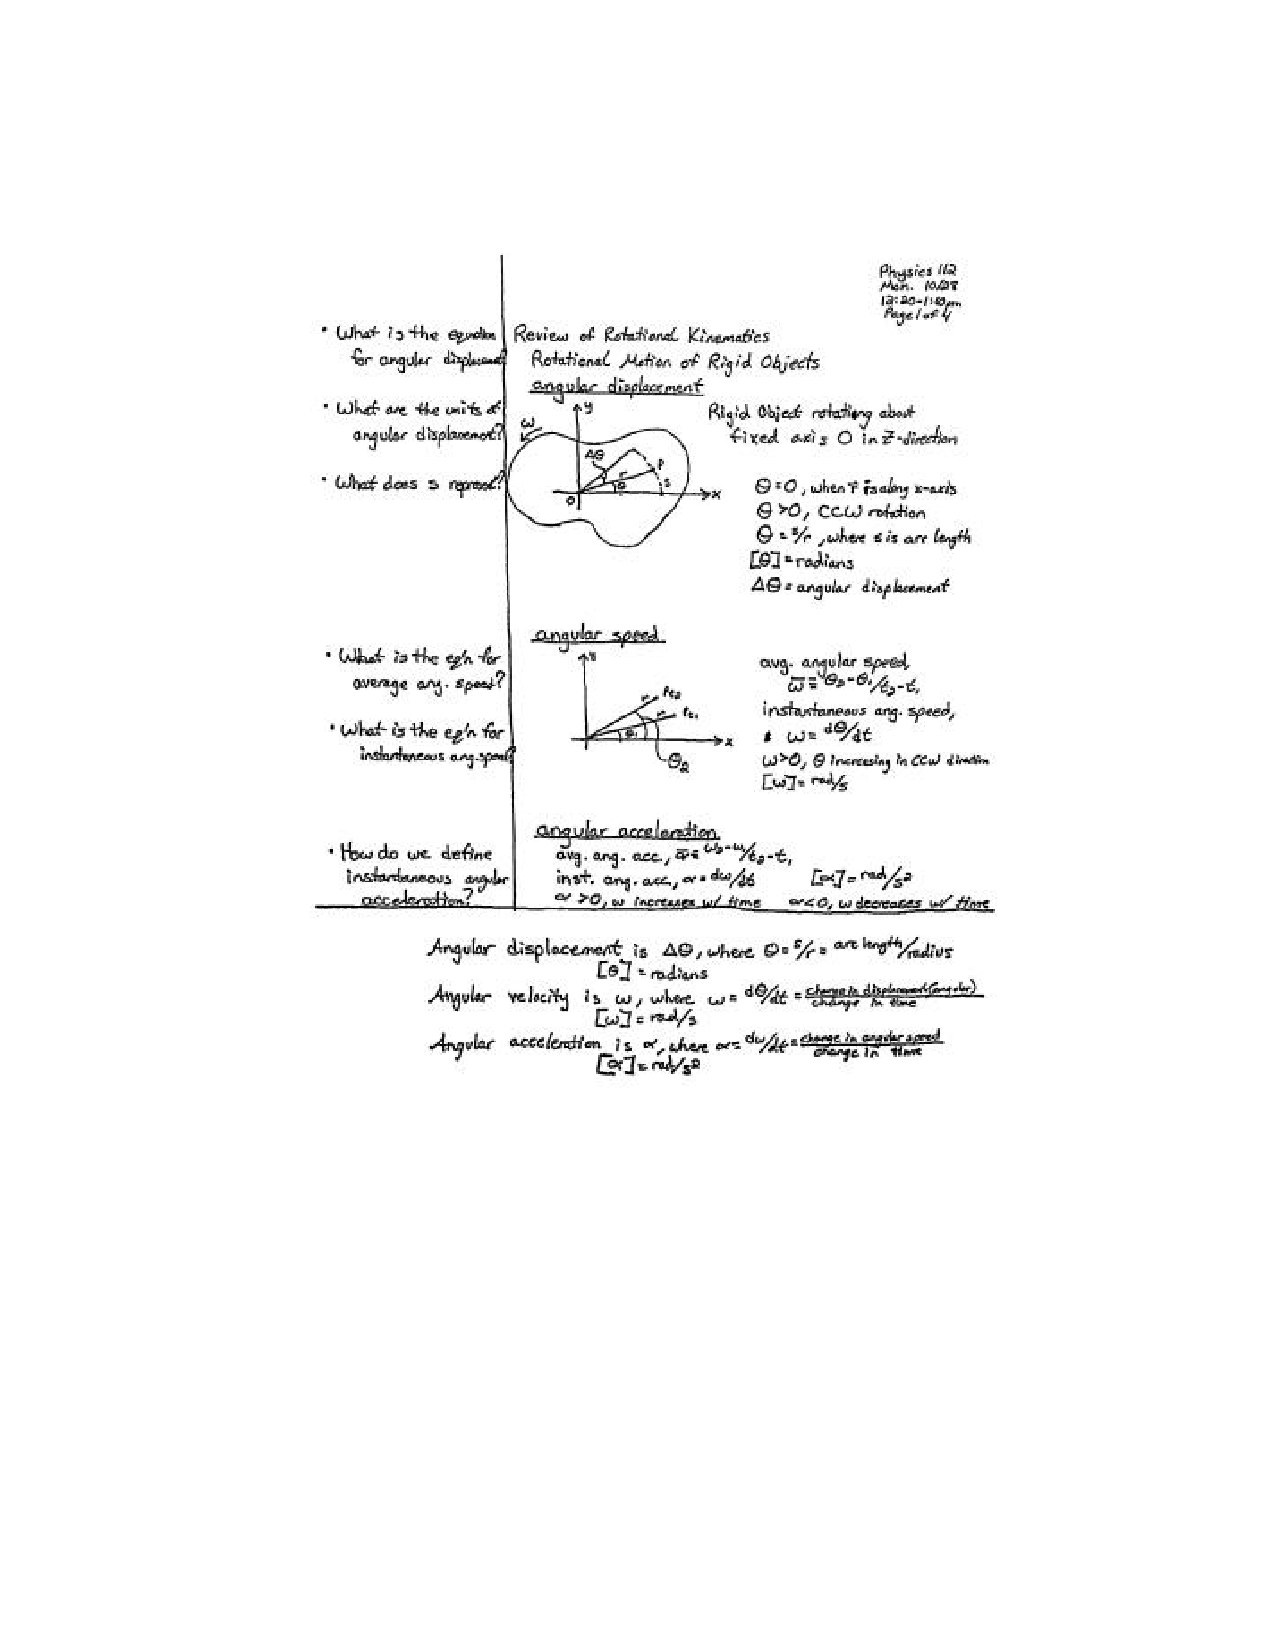
\includegraphics[height=8cm]{./images/00/Cornell-NTS/exCNTS.pdf}
	\end{center}
	
	笔记的行程过程可以分为所谓的{\bf 5R}:
	
	\begin{enumerate}[Step1]
	  \setlength{\itemindent}{1cm}
	  \item {\it 记录(Record):}在听讲或阅读过程中,
	  在主栏(将笔记本的一页分为左大右小两部分,
	  左侧为主栏,右侧为副栏)内尽量多记有意义的论据、概念等讲课内容。
	  \item {\it 简化(Reduce):}下课以后,尽可能及早将这些论据、概念简明扼要地概括(简化)
	  在回忆栏,即副栏。
	  \item {\it 背诵(Recite):}把主栏遮住,只用回忆栏中的摘记提示,
	  尽量完满地叙述课堂上讲过的内容。
	  \item {\it 思考(Reflect):}将自己的听课随感、意见、经验体会之类的内容,
	  与讲课内容区分开,写在卡片或笔记本的某一单独部分,加上标题和索引,
	  编制成提纲、摘要,分成类目。并随时归档。
	  \item {\it 复习(Review):}每周花十分钟左右时间,快速复习笔记,主要是先看回忆栏,
	  适当看主栏。
	\end{enumerate}
	
	在课本、参考书原文的旁边加上各种符号(如直线、双线、黑点、圆圈、
	曲线、箭头、红线、蓝线、三角、方框、着重号、惊叹号、问号等等),便于找出重点,
	加深印象,或提出质疑。什么符号代表什么意思,自己掌握即可,但最好形成一套比较
	稳定的符号系统。这种方法特别适合于自学笔记和预习笔记。
	
	操作时注意以下一些准则:
	{\it 读完后再做记号,要非常善于选择,用自己的话进行注记,形式和过程力求简洁,迅速,整齐}
	
	笔记的加工:{\it 忆$\to$补$\to$改$\to$编$\to$分$\to$舍$\to$记}	
\end{shaded}


% \chapter{函数与极限}

极限是微积分理论中最基础的概念(定义和讨论微分和积分的基础),理解极限的数学
定义与性质,掌握极限收敛判定和极限计算的方法,是真正深入理解微积分的第一步。

极限的数学定义(更具体地称为“$\e-\delta$”或“$\e-N$”定义)是进入微积分学习
后可能遇到的第一个难点(难度可能因人而异),因为它兼具形式的抽象性和逻辑的复杂性
(因为必须严谨、准确)。学会用数学和逻辑的语言表达某个概念、性质和进行推理、分析,
也是通过微积分的学习需要锻炼和培养的能力。从这个角度来说,极限概念的重要性就更加
不言而喻了。

% {\bf 关键词:}集合、集合论、映射、函数、曲线及其表示

% \setcounter{section}{-1}

\section{集合、映射与函数}

\subsection{集合}

{\it Cantor,1874:}\ps{对于集合,“我们只需描述它,而不必给出精确的定义”}
所谓{\it 集合},是指把一些个体({\it 元素}) 放在一起考虑时它们形成的整体。
\begin{itemize}
  \setlength{\itemindent}{1cm}
  \item 关系符号:$\subset, \in, =, \subseteq, \neq$
  \item 运算符号:$\cap,\cup, \setminus, \bar{A}, \times, +, - $\quad ({\it
  依次为:交、并、差、补、笛卡尔积、不交并、差})
\end{itemize}
	
本门课程中常见(用)的集合:
$$\b\mathbb{N}\subset\mathbb{Z}\subset\mathbb{Q}
\subset\mathbb{R}\subset\mathbb{C}$$
\quad({\it 依次为:自然数集\ps{\b 国内教材一般约定,自然数集包含数$0$}、
整数集\ps{德语Zahlen(数)的首字母}、有理数集、无理数集和复数集})


通过集合的{\it 笛卡尔积}“$\times$” 可以定义更{\it
“高维”}的集合,例如:$\mathbb{R}$表示数轴(上的所有点构成的集合),则
$${\b \mathbb{R}^2=\mathbb{R}\times\mathbb{R}}$$
表示全平面(上的所有点构成的集合)

{\bf 【区间和邻域】}

{\bf 例:}给定$a,b\in\mathbb{R},a<b$,区间$(a,b)=\{x\in\mathbb{R}|a<x<b\}$

{\bf 例:}记实数集$\mathbb{R}=(-\infty,+\infty)$

{\bf 注意:}{\b 由于$\pm\infty$都不是具体的数,因此在本门课程中,除非特别说明,形如
\ps{\b 请对讲义中蓝色字体的部分多加留意!}
$$x=+\infty\quad\mbox{或}\quad x=-\infty$$
的写法总是错误的,而只能写
$$x\to+\infty\quad\mbox{或}\quad x\to\infty$$
}

{\bf 邻域}
$${\b U(a,\delta)}=(a-\delta,a+\delta)=\{x\in\mathbb{R}||x-a|<\delta\}$$
含义为:实数集中所有与$a$绝对值小于(距离小于)$\delta$的数(点)构成的集合

{\bf 例:}
$$(a,b)=U\left(\df{a+b}2,\df{b-a}2\right)$$

{\bf 去心邻域}
%\ps{同济写做$U^0(a,\delta)$,我们在使用是可不加区别}
$${\b
U_0(a,\delta)}=(a-\delta,a+\delta)-\{a\}=\{x\in\mathbb{R}|0<|x-a|<\delta\}$$

{\bf 无穷邻域}*\ps{名词后面加星号的,表示了解即可}
$$\{x\in\mathbb{R}||x|>M\},\;M>0$$

{\bf 问:}以上无穷邻域可以写成类似$U(\infty,M)$的形式吗?

答:因为$\infty$不是一个具体的数(点),
所以为了避免误解,我们不会这么写!

{\bf 半邻域,左(右)邻域},例如:点$a$的右半邻域为
$$\{x\in\mathbb{R}|a<x<a+\delta\}$$

\ps{灰色背景内容为扩展知识,了解即可}

\begin{shaded}

{\bf 集合论、Russell Paradox与公理系统}

	{\it Cantor,1874:}朴素集合论的诞生。	

	{\it Poincare,1900,国际数学家大会:} 
		 {“\ldots 借助集合论概念,我们可以建造整个数学大厦\ldots  今天,我们可以说绝对的严格性已经达到了\ldots”}
	
	{\it Russell, 1901:}只给不给自己理发的人理发的理发师该不该给自己理发?
	
	“由所有不包含集合自身的集合所构成的集合”,记为$S$。不论$S$是不是自身的元素,按照$S$的定义都会有矛盾。
	
	设$x\in A$表示:$A$给$x$理发, 定义
	$$A=\{x|x\notin x\},$$ 
	
	问:$A\in A$还是$A\notin A$? 
	
% 	\ba{罗素悖论导致了第三次“数学危机”的出现!}
	{{\bf {第三次“数学危机”}}(Frege,1901,《算术基础》)}
		“在工作结束之后发现那大厦的基础已经动摇,对于一个科学工作者来说,没有比这更不幸的了”
		
	\begin{itemize}
	  \item {{\bf 无限抽象原则}(Cantor,Frege):} 任意给定某个条件就可以确定一个集合。(每个概念的外延可以确定一个集合)
	  \item {\bf 观点:}不加限制地使用无限抽象原则将导致罗素悖论
	  \item {{\bf 有限抽象原则}(限制公理):} 如果已知一个集合和一个给定的条件,
	  则该集合中所有满足条件的元素{\it 可以}构成一个集合。
	  \item {\bf ZF(Zermelo-Fraenkel)公理化集合论}
	  (Zermelo-Fraenkel Set Theory):包含选择公理的称ZFC,否则为ZF。
	  
	  {\bf 命题:}在ZF/ZFC中,无法定义包含所有集合的集合。
	
	[证]:反证法。设$A$是一个这样的集合。定义
	$$B=\{x\in A|x\notin x\}$$
	若
	$B\in A$,则必有$B\in B$或$B\notin B$。而若$B\in B$,可推出$B\notin B$;同理,
	由$B\notin B$,也可推出$B\in B$。从而$B\notin A$,推出矛盾。这说明$B$的定义存在问题,故知假设错误。

	\item {\bf 公理(Axiom):}无须证明即为正确的命题。
	\begin{itemize}
	  \item {\it Engles:}数学上的所谓公理,是数学需要用作自己出发点的少数思想上的规定 
	  \item {\bf ZFS系统:}公理就是一些关于逻辑符号{“$\in$”}和{字母}的组合使用方法的约定
	  \item {\bf 公理化方法}是构建现代数学理论体系的基石
	\end{itemize}
	\item {\bf {数学等于永恒的真理吗?}}
	\end{itemize}
	
	{\bf 注:}ZFC有无穷多个公理,因为替代公理实际上是公理模式。已知ZFC和ZF集合论
	二者都不能用有限数目个公理来完全公式化。
	
	{\bf 讨论:}公理(Axiom)、定理(Theorem)、定律(Law)、假设(Assumption)、
	引理(Lemma)、推论(Corallary)、猜想(Conjuction)有何异同?
	{\b\dotfill\it 建议做常识性了解!}
	
	{\it 试答:这些概念都是对自然规律或数学规则的表达。
	
	公理是数学及其相近领域所使用的概念,即在数学理论体系中无须证明即视为正确的命题(例如:
	两点之间直线最短),是数学理论体系的出发点。通过推理和演绎,我们可以在公理的基础上
	进一步推出新的结论,这些结论我们通常称为定理,引理和推论则是定理推导的中间和后续结果。
	使用不同的公理作为出发点,可能得到完全不同的理论体系,例如:非欧几何的多条基本公设(公理
	的另一种说法)就是和欧式几何不同的,这导致二者的理论体系看起来大相径庭。
	
	我们目前所使用的公理多数来源于生活中的直观体验,是一种对直觉观察的抽象描述。而由于
	我们对自然世界认识的局限性,这些描述本身可能是不精确甚至是不正确的。从这个意义上说,我们
	更应该说公理其实是我们对于客观规律的假定,是先验的,但也是可以有所调整和变化的。
	
	定律也具有类似的特点,因为人类总是在不断改进和加深对于自然世界的认识。定律更多
	地出现于物理、化学等非抽象领域,体现的是对自然规律的描述。定律背后通常存在一些的
	基本假定(例如:原子是不可分的、光既是例子又是波),定律的发现需要以重复实验为基础,
	定律的描述中一部分是可以用数学工具来刻画的(例如万有引力定律、质能方程)。
	
	公理、定理、定律的共性之处在于它们在各自的领域中或背景下,都被视为是“正确的”(请注意在数学中
	正确和可证明有时是被混同的),是被验证、证明或直接假定为真的命题,而猜想则是被
	猜测为真,但未经过这些过程,所以仍无法断言为真的。当今的数学界,仍有大量的猜想有待证明或证否,
	这些问题所代表的恰恰是数学的最前沿。
	}
\end{shaded}
	
{\bf 【实数集的性质】}
	\begin{thx}
		\begin{enumerate} 
		  \item {\bf 有序性:}即任何两个实数均可以比大小\quad (注:$\mathbb{R}^2$、$\mathbb{C}$不具备有序性) 
	% 	  \ps{$\mathbb{R}$是全序的,而$\mathbb{R}^2$、$\mathbb{C}$在一定的度量下
	% 	  是半序的}
		  \item {\bf 完备性(连续性): }实数集与数轴上的点之间存在一一对应
	% 	  \ps{这是KD教材上的说法,不够严谨!}
			
		  {\bf{连续性公理(确界原理):}}非空有{上界}的实数集必有{上确界} (最小的上界)
		\end{enumerate}
	\end{thx}
	
	  {\bf 注}:实数集的完备性更准确的说法应该是:
	  {\it 实数集的任意非空有上界的子集都有上确界,且该上确界为实数}
	
	为了更好地理解确界原理,必须对集合的有界性以及上(下)界和上(下)确界的概念有非常准确的理解:
	
	\begin{thx}
		{\bf 上界:}$M\in\mathbb{R}$称为集合$A\subset\mathbb{R}$的上界,是指:对任意$x\in A$,均有
		$x\leq M$。
		
		{\bf 集合$A$有上界:}存在$M\in\mathbb{R}$为$A$的上界(显然上界是不唯一的!)
		
		{\bf 集合$A$有界:}即$A$同时有上下界。
	\end{thx}	
	
		设$M$和$m$分别为$A$的上界和下界,令$M^*=\max\{|m|,|M|\}$,则可以证明,对
		任意$x\in A$,有$-M^*\leq x\leq M^*$,或$|x|\leq M^*$。这个命题
		也常常作为集合有界的定义。
	\begin{thx}
		{\bf 上确界:}{\b
		$M_0\in\mathbb{R}$称为集合$A\subset\mathbb{R}$的上确界
		(记为$M_0=\mathrm{sup}A$,下确界记为:$\mathrm{inf}A$),
		是指:$M_0$是$A$的最小上界},也即同时有:
		\begin{enumerate}[(1)]
		  \setlength{\itemindent}{1cm}
		  \item $M_0$是$A$的上界,即:对任意$x\in A$,均有$x\leq M_0$;
		  \item $A$的任意上界都不小于$M_0$,即:若$M$为$A$的一个上界,则$M_0\leq M$。
		\end{enumerate}
		{\bf $M_0$为$A$的上确界}的另一个{\it 数学定义}:对任意小的$\e>0$,
		都存在某个与之对应的$x_{\e}\in A$,使得$M_0-\e<x_{\e}\leq M_0$,
		或者简写作
		$$M_0=\mathrm{sup}A\;\Leftrightarrow\;
		\forall\e>0,\;\exists x_{\e}\in A,\;M_0-\e<x_{\e}\leq M_0.$$
	\end{thx}

	{\bf 思考:}上面这个对上确界的数学定义
	\ps{大多数时候,我们并不严格区分{\b 数学定义}和{\b 概念},只是数学定义通常
	会用更抽象的数学符号和更严谨的逻辑语言来表达,今后我们所说的{\b 定义}即指
	数学定义或概念}
	,与前面我们讨论的上确界的概念之间	是什么关系?你能否证明它们是等价的?
	
	{\bf 思考:}上确界和最大值有什么异同?如何确定一个集合的上确界?
	
	{\bf 讨论:}{\b 有理数集不满足连续性公理!}准确地说就是:有理数集的非空有上界的子集,
	其上确界未必是有理数	(但肯定是实数)!为了说明这一点,来看下面的例子:
% 	\ps{如果将取上确界视为一种集合运算,这里所说的完备性可以理解为,
% 	该集合对于取上确界的运算封闭}
	
	{\bf 例:}考虑集合$A=\left\{\left(1+\frac 1n\right)^n|n\in\mathbb{N}\right\}$,因为
	有理数的有限次四则运算仍是有理数,故显然$A\subset\mathbb{Q}$。如下图所示,集合$A$中的点如果按照
	$n$从小到大的顺序排列,恰好是构成一个随$n$单调递增有上界($3$就是它的一个上界)的数列,也即:
	$$\left(1+\frac11\right)^1<\left(1+\frac12\right)^2<\left(1+\frac13\right)^3<\ldots
	\left(1+\frac1n\right)^n<\ldots<3,$$
	\begin{center}
		\resizebox{!}{6cm}{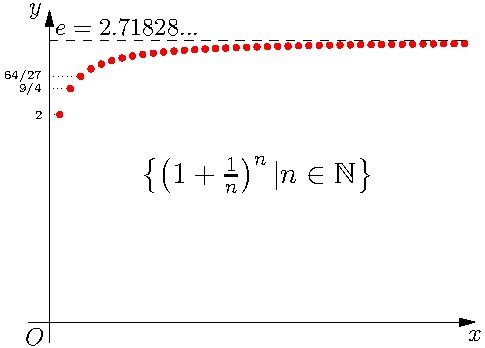
\includegraphics{./images/ch1/e-notin-N.pdf}}
% 		\resizebox{!}{4.8cm}{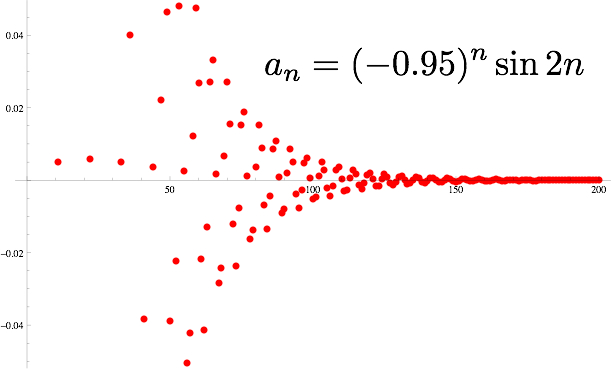
\includegraphics{./images/ch2/sin2nn.jpg}}
% 		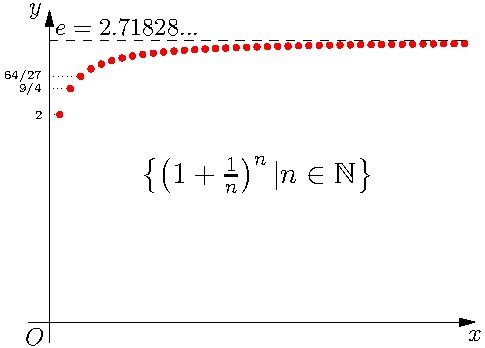
\includegraphics[width=6cm]{./images/ch1/e-notin-N}
	\end{center}
	根据常用极限\ps{稍后就会学到}
	$$e=\lim\limits_{n\to\infty}\left(1+\df1n\right)^n,$$
	不难看出$e=\mathrm{sup}A$。由于$e\notin\mathbb{Q}$,故有理数集不满足连续性公理。
	
	又比如下面的例子:
	
	{\bf 例:}$A=\{x\in\mathbb{Q}|x\geq 0,\;x^<2\}$,显然,
	$\mathrm{sup}A=\sqrt2\notin\mathbb{Q}$。
	
	{\bf 思考:}任给一个实数,如何构造一个有理数集合,使得该实数恰好为
	该有理数集合的上(下)确界?
	
	\begin{shaded}
	{\bf 开集与闭集}
	
	集合$A\subset\mathbb{R}$为{\bf 开集},是指:对任意$x\in A$,均存在$\delta>0$,使得
	$U(x,\delta)\subset A.$
	
	集合$A\subset\mathbb{R}$为{\bf 闭集},是指其补集$\bar{A}=\mathbb{R}-A$为开集。
	
	例如:所有的开区间都是开集,所有的闭区间为闭集;我们通常{\it 约定空集$\phi$既是开集又是闭集,
	因此{\b 实数集$\mathbb{R}$既是开集又是闭集}}。
	
	点$a$称为集合$A$的{\bf 内点},是指:存在$\delta>0$,使得$U(a,\delta)\subset A$。显然开集中的点均为其内点!
	
	点$a$称为集合$A$的{\bf 外点},是指:存在$\delta>0$,使得$U(a,\delta)\cap A=\phi$,
	或者说$a$为$A$的补给的内点。
	
	点$a$称为集合$A$的{\bf 边界点},是指$a$既不是$A$的内点,也不是$A$的外点,或者说
	对任意的$\delta>0$,$U(a,\delta)\cap A\ne\phi$。
	
	显然,闭集可以视为其最大开子集和其所有边界点的并。
	
	{\bf 例:}以下集合哪些是开集,哪些是闭集?
	\begin{enumerate}[(1)]
	  \setlength{\itemindent}{1cm}
	  \item $\{1,2,3,5\}$\quad\quad({\it 闭})
	  \item $U_0(1,3)$\quad\quad({\it 开})
	  \item 自然数集\quad\quad({\it 闭})
	  \item 有理数集\quad\quad({\it 既非开又非闭})
	  \item 无理数集\quad\quad({\it 既非开又非闭})
	  \item $\left\{\left(1+\frac
	  1n\right)^n|n\in\mathbb{N}\right\}+\{e\}$\quad\quad({\it 闭})
	\end{enumerate}
	
	\end{shaded}

\subsection{映射}

映射通常被定义为,事物之间“一对一”或“多对一”的依赖关系。更形象地说,可以将
映射视为一种输入输出过程,“一对一”或“多对一”保证了
一个输入只能得到一个特定的输出,因此结果是{\it 无歧义}
\ps{无歧义是保证数学论证简明性的一个常见的要求}
的。从这个意义上说,对于映射的这种定义方式也是一种{\it 约定}。
由集合$A$到$B$的映射$f$一般记为:

$$f:A\mapsto B \quad\mbox{或}\quad y=f(x),\;x\in A,y\in B$$

{\it 映射的三要素:}定义域、值域、对应关系,任何一项不明确都不足以确定一个函数,或者说,
两个映射在这三方面有一点不同,则应视为不同的映射。
\ps{之所以有时候只关心定义域和对应关系,前提是默认假设映射为满射}

{\bf 函数}通常是指实数集(的子集)之间的映射。有时也推广到高维的实数集,例如
$$z=x^2+y^2,\;(x,y)\in\mathbb{R}^2.$$

{\bf 例:}假设下列函数均取{\it 自然定义域}\ps{即在$\mathbb{R}$中最大的定义域},
且均为满射,指出其中哪些是完全相同的?
		$$x,\quad |x|,\quad e^{\ln x},\quad \ln(e^x),\quad \sqrt{x^2},\quad
		\frac{x^2-4}{x-2}-2,$$
		$$\sin(\arcsin x),\quad \arcsin(\sin x), \quad \tan(\arctan x)$$

相关概念:{\bf 单射、满射、一一映射(双射)}

\begin{shaded}
	{\bf 一一映射与无穷集合}
	
	{\bf 问题:}如何比较两个集合中元素的个数({\it 元素有限的情况下通常称为“度”})?
	
	答:如果存在集合$A$和$B$之间的一一映射,则称$A$和$B$是{\it 等势}的。
	
	{\bf 例:}以下集合两两等势吗,为什么?({\b 正确的命题须给出证明,错误的给出证明或举反例})
	\begin{enumerate}[(1)]
	  \setlength{\itemindent}{1cm}
	  \item 自然数与正偶数({$\surd$})
	  \item 自然数与整数({$\surd$})
	  \item 自然数与有理数({$\surd$})
	  \item 区间$(0,1)$中的实数与$\mathbb{R}$中({$\surd$},例如:$y=\df1{e^x+1}$)
	  \item 自然数与实数({$\times$})
	\end{enumerate}
	
	[提示]:(2)\;一个集合与自然数集等势,等价于这个集合中的所有数可以不重复地
	排成一列,形象地说,就是可以把这个集合中所有的数一个个地数完而没有任何重复
	与遗漏。例如要证明整数集与自然数集等势,显然只需这样来排列整数集:
	$$0,1,-1,2,-2,3,-3,4,-4,\ldots,$$
	很容易看出这样的排列是既没有遗漏也没有重复的,事实上等于给出了从自然数集到
	整数集的一一映射。
	
	(3)\;参照上面的作法,要证明自然数集与有理数集等势,也只需要考虑能否找到一种方式
	将所有的有理数排成一列,既不重复也不遗漏。参考下图,我们可以先说明所有的正有理数
	可以排成一列:
	\begin{center}
		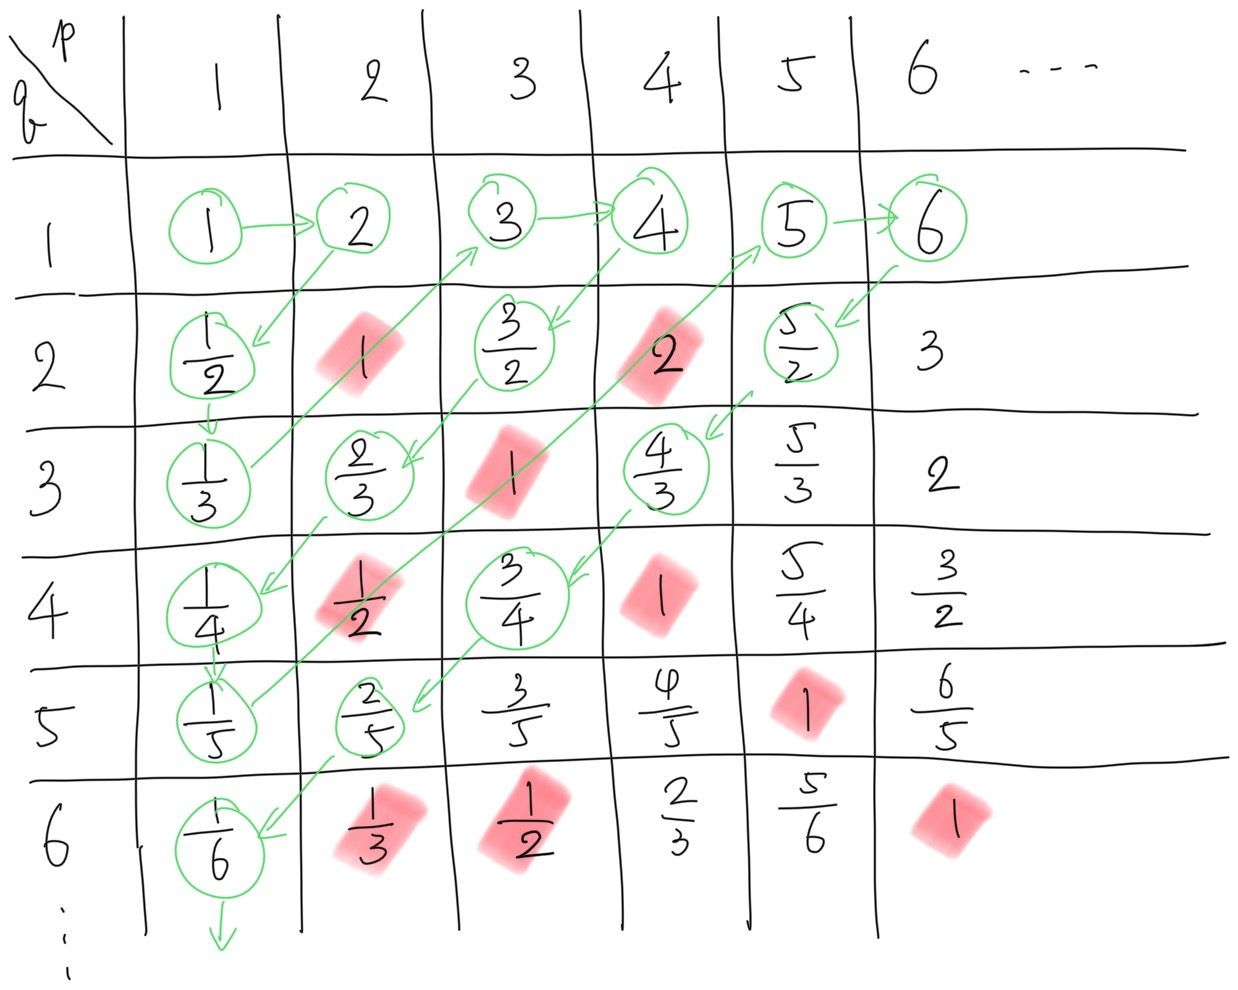
\includegraphics[width=8cm]{./images/ch1/Qp.jpg}
		
		{\it 表格中列出了所有的正有理数,红色覆盖的是重复出现的数字}
	\end{center}
	$$1,2,\df12,\df13,3,4,\df32,\df23,\df14,\df15,5,6,\df52,
	\df43,\df34,\df25,\df16,\ldots,$$
	从图上不难看出,这个排列事实上给出了从自然数集到正有理数集的一一映射。
	接下来,在其中逐个插入对应的负有理数,即可得到从自然数集到有理数集的
	一一映射。
	
	(5)\;了解了(4)的结论,我们只需证明不存在自然数集到区间$(0,1)$的一一
	映射即可。
	
	我们采用反证法:假设存在自然数集到$(0,1)$的
	一一映射,这意味着$(0,1)$中所有的数可以排成一个数列,没有重复也没有遗漏,
	其中第$i$个数表示为
	$$a_i=a_{i1}a_{i2}a_{i3}a_{i4}\ldots,$$
	其中$a_{ij}(j=1,2,\ldots)$都是$0$到$9$之间的个位整数。
	
	接下来,我们构造一个新的数
	$$a_*=a_{*1}a_{*2}a_{*3}a_{*4}\ldots,$$
	其中$a_{*j}(j=1,2,\ldots)$也都是$0$到$9$之间的个位整数,同时满足
	$$a_{*j}\ne a_{jj},\; j=1,2,3,\ldots.$$
	
	从$a_*$的构造特点上,我们可以得出如下两个结论:
	\begin{enumerate}[(i)]
	  \setlength{\itemindent}{1cm}
	  \item $a_*\in(0,1)$,
	  \item $a_*\ne a_i,\;i=1,2,3,\ldots$
	\end{enumerate}
	由于根据我们的假设,数列$\{a_i\}$中已经不多不少地包含了$(0,1)$中所有的数,因此
	以上第二条恰好说明$a_*\notin(0,1)$,这就出现了矛盾。从而可以断言
	假设错误,也就是说,不存在自然数集到$(0,1)$的一一映射,因此二者
	不等势,最终得到结论自然数集与实数集也不等势。
	
	上面这些结论反映出一个有趣的现象,就是有些集合可以和自己的真子集建立起
	一一映射。	Cantor敏锐地抓住了这一点,并认为应该是{\b\it 无穷集合}本质
	特征,进而第一次给出了无穷集合的定义
	\begin{tcolorbox}
		{\bf 无穷集合:}可以和自身的某个子集建立起一一映射的集合
	\end{tcolorbox}
	历史上,Cantor曾被人称为“{\it 数学史上最富于想象力的最具争议的人物之一}”、
	拥有“{\it 对于提出深刻的问题以及不时探索始料未及的解法以至寻求非正统答案的天赋}”。
	他的名言也是信条是“{\it 数学的本质在于它超然的自主性}”。
\end{shaded}	

\subsection{函数}
	
% 	\begin{shaded}
% 		{\bf 关于函数}
% 		\begin{itemize}
%   		  \setlength{\itemindent}{1cm}
% 		  \item 微积分是关于运动和变化的数学;
% 		  \item 函数是对运动(例如:曲线、曲面、波以及各种变化)变化过程中各种量与量的依赖关系的抽象描述;
% 		  \item 函数刻画了运动变化中的量之间的相互依存关系({\bf 注:}与“依存”对应的关系叫做“独立”)
% 		\end{itemize}
% 		
% 		{\bf 常量和变量}
% 		\begin{itemize}
%   		  \setlength{\itemindent}{1cm}
% 		  \item {\it 常量和变量是相对的},在一定条件下可以相互转化
% 		  \item 变量之间的关系可能是相互依存,也可能是相互独立的
% 		  \item 为了避免讨论过于复杂,简化问题,我们可能选择只考虑部分参数的变化,而将其他参数视为(或设为)常量,
% 		  例如:万有引力与两个物体的质量、距离以及引力常数(系数)都有关,为了确定其数量关系,需要事先假定部分的参数
% 		  值是固定不变的
% 		\end{itemize}
% 		
% 		{\bf 大学数学 vs. 中学数学}
% 		\begin{itemize}
%   		  \setlength{\itemindent}{1cm}
% 		  \item 数学并无严格的{\it “高等”}和{\it “初等”}之分,只是存在众多的分支和领域
% 		  (例如:代数、几何、分析、图论,几何又分为平面几何、立体几何、解析几何等),
% 		  不同分支或领域的直观性和难度各有不同
% 		  \item 对于函数,中学阶段更注重在对应关系“确定”的情况下,寻找其数学描述或利用给定的值进行计算
% 		  \item 大学阶段,从微积分开始,更着重对函数的特性(如导数、积分、曲率),
% 		  不同函数间的转换、类比,以及关于函数整体特征的计算与分析
% 		\end{itemize}
% 		
% 		 {\bf James Stewart, Calculus(5th eds.), 2004}
% 		  \begin{itemize}
%   		    \setlength{\itemindent}{1cm}
% 		    \item {\it Calculus is fundamentally different from the mathematics that
% 		    you have studied previously}
% 		    \item {\it Calculus is less static and more \underline{dynamic}
% 		    :微积分更加关注动态多余静止}
% 		    \item {\it It is concerned with change and \underline{motion}
% 		    :研究的对象是运动和变化}
% 		    \item {\it It deals with quantities that \underline{approach} 
% 		    other quantities
% 		    :关注数量之间的相互趋近}
% 		  \end{itemize}
% 	\end{shaded}
	
	函数是微积分研究的基本对象,不同于中学阶段,以对函数值的讨论和计算为重点,
	微积分更关注函数的变化特征(如导数与高阶导数、曲率)与整体性质(如连续性、
	定积分)。
	
	{\bf (一元)函数:}由实数集到实数集的映射
	$$f:D\mapsto\mathbb{R},\;(D\subset\mathbb{R})$$
	或
	$$y=f(x),\quad (x\in D\subset\mathbb{R},y\in\mathbb{R})$$
% 	\begin{itemize}
% 	  \item {\bf 定义域:} $D\subset \mathbb{R}$ ,且$D\ne\phi$ 
% 	  \item {\bf 对应关系:} $f:D\to\mathbb{R}$
% 	\end{itemize} 
	
	{\bf (一元函数的)函数图像:}
	$$G=\{(x,f(x))\in\mathbb{R}^2|x\in D\}$$
	
	\begin{shaded}
		{\bf 多元函数:} 
		$$f:D\to\mathbb{R},\quad D\in\mathbb{R}^n$$
		
		{\bf 向量值函数:}
		$$f:D\to\mathbb{R}^n,\quad, D\in\mathbb{R}$$
		
		{\bf 思考:}二元函数和三维的向量值函数可以表示怎样的几何对象?
	\end{shaded}
	
	\begin{center}
		\resizebox{!}{4.2cm}{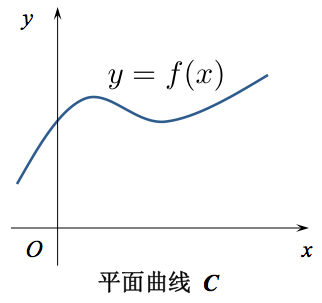
\includegraphics{./images/ch1/C_fx.jpg}}\quad	
		\resizebox{!}{4.5cm}{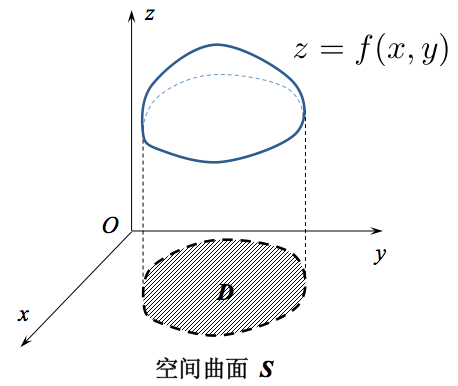
\includegraphics{./images/ch1/S_fxy.jpg}}
	\end{center}
	
	{\bf 思考:}{\b 平面曲线与一元函数具有一一对应关系吗?}空间曲面和二元函数呢?
	
	答:不是的,例如圆$x^2+y^2=1$如果写成一元函数形式,需要至少两个函数
	$y=\pm\sqrt{1-x^2}$。空间曲面和二元函数的关系与之类似,例如空间球面
	$x^2+y^2+z^2=1$也至少需要写成两个$z$关于$x,y$的二元函数
	$z=\pm\sqrt{1-x^2-y^2}$。
	
	由于以上问题的存在,为了表示平面曲线(空间曲面),我们会用到其他一些的曲线方程,
	例如:单位圆的方程也可以写为:\ps{关于参数方程和极坐标方程的介绍,参见KD教材1.3节}
	\begin{itemize}
%   		\setlength{\itemindent}{1cm}
		\item {\bf 隐函数方程}:$x^2+y^2=1$
		\item {\bf 参数方程}:$(x,y)=(\cos t,\sin t),\quad t\in[0,2\pi]$
		\item {\bf 极坐标方程}:$\rho=1,\theta\in[0,2\pi]$
	\end{itemize}
	
\subsubsection{函数的运算}

% {\bf 基本的函数运算}
% \ps{\b 因为无穷次的函数四则运算和复合可能导致一些特殊的函数性质出现,
% 以下如未特别说明,所列出的运算次数均为有限的}
\begin{enumerate}
  \setlength{\itemindent}{1cm}
  \item {\it 四则运算:}$+,-,\cdot,/$
  \item {\it 复合运算:}函数的复合运算就是中间变量的代入过程,$(f\circ g)(x)=f(g(x))$
  \item {\it 逆运算:}函数求逆(反函数)要注意反函数存在的条件:$f$为{\it 双射}
\end{enumerate}

{\bf 问:}$y=f(x)$和$x=f^{-1}(y)$的图形的关系是怎样的?({\it 答:相同!})

\subsubsection{函数的简单性质}
	
\begin{tcolorbox}[colback=white!90!black]
	{\bf 常用的简写符号:}约定用于数学推导中一些常用文字的书写替代,汉英通用
	\begin{itemize}
% 	  \setlength{\itemindent}{1cm}
	  \item {\b$\bm{\forall}$} \quad 任意 (for all, arbitrary)
	  \item {\b$\bm{\exists}$} \quad 存在 (exist)
	  \item {\b$\bm{\Rightarrow}$} \quad 推出 (deduce, imply)
	  \item {\b$\bm{\Leftrightarrow}$} \quad 等价、当且仅当 (equivalent, if and only if)
	  \item {\b$\bm{\to}$} \quad 趋于 (approach)
	\end{itemize}
\end{tcolorbox}

{\bf 【有界性】}			

	设$I\subset\mathbb{R}$,$f(x)$在$I$上有定义,若集合
	$\{f(x)|x\in I\}$	有界,则称{\it $f(x)$在$I$上有界}
	或{\it $f(x)$是$I$上的有界函数}
	\ps{函数的有界性就是其值域的有界性}

	{\bf 例:}判断以下函数在其定义域上的有界性
	\ps{注意掌握这几个函数图形的大致轮廓}
	
	\quad(1)\;$y=x\sin x$,\hspace{5em} (2)\;$y=\df{\sin x}x$,
	\hspace{5em} (3)\;$y=\sin\df1x$
		
	\begin{center}
		\resizebox{!}{4cm}{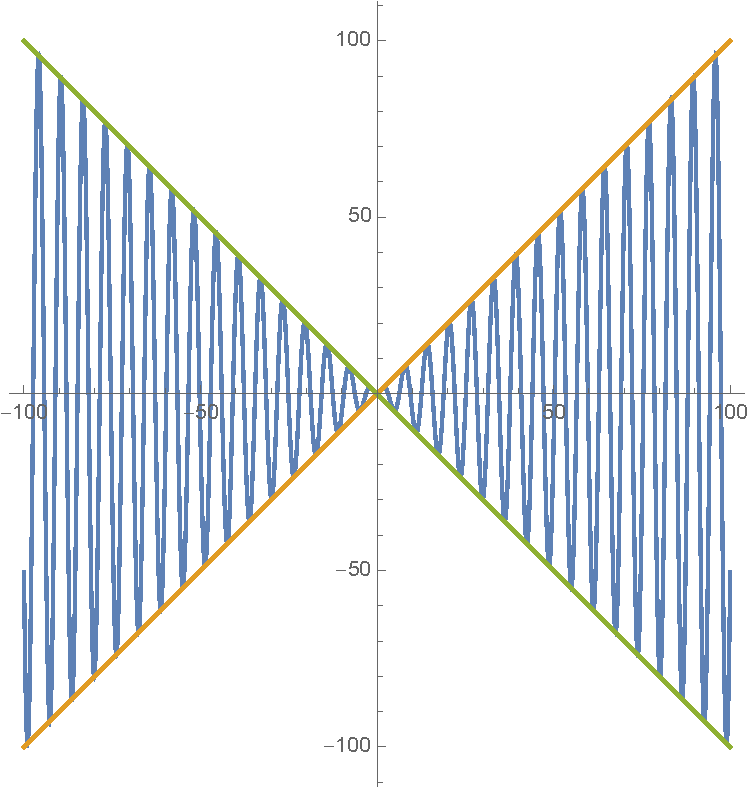
\includegraphics{./images/ch1/xsinx.pdf}}
		\resizebox{!}{3cm}{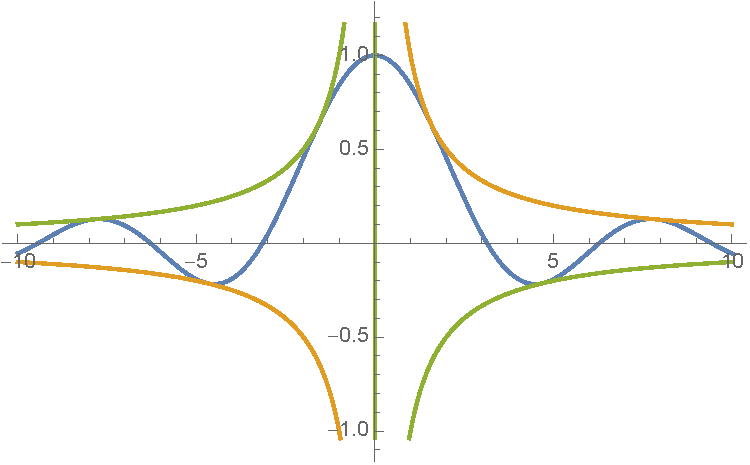
\includegraphics{./images/ch1/1xsinx.pdf}}	
		\resizebox{!}{3cm}{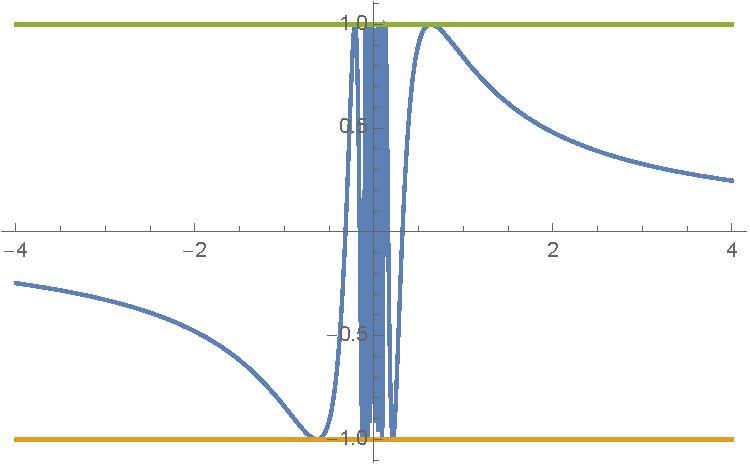
\includegraphics{./images/ch1/sin1x.pdf}}
	\end{center}
	
\begin{shaded}
	{\bf “反面定义”(否命题)的写法:}对命题中的如下文字进行相互替换
	\begin{enumerate}
	  \setlength{\itemindent}{1cm}
	  \item {\b “任意”与“存在”}
	  \item {\b “$\geq(\leq)$”与“$<(>)$”}
	  \item {\b “和”与“或”}
	\end{enumerate}
	
% 	[提示]::参考De Morgen律,任何命题的成立都是与一定范围有关的
	以函数的有界性为例,其否命题为函数无界。
	
	\begin{tcolorbox}
		{\it $f(x)$有上界}:{\b\it 存在}$M\in\mathbb{R}$,对
		{\b\it 任意}$x\in D$,有$f(x){\b \leq} M$。
		
		{\it $f(x)$有上界}:对{\b\it 任意}$M\in\mathbb{R}$,{\b\it 存在}$x_M\in
		D$,使得$f(x_M){\b >}M$。
	\end{tcolorbox}
	
	{\bf 例:}用以上关于函数无上界的定义,证明$y=x\sin x$无界。
	
	注:所谓{\it 用定义证明}函数的性质,就是验证该函数满足这个定义中的命题
	
	[证]:对任意$M\in\mathbb{R}$,
	令$x_M=\left(\left[\df{M}{2\pi}\right]+1\right)
	\cdot2\pi+\df{\pi}2$(其中$[x]$为{\it 下取整函数},表示不大于$x$的最大整数,
	显然$[x]\leq x<[x]+1$),	则有
	$$x_M>\df{M}{2\pi}\cdot2\pi+\df{\pi}2>M,\quad\mbox{且}\quad \sin x_M=1,$$
	故
	$$x_M\sin x_M=x_M>M.$$
	从而根据函数无上界的定义,可知该函数无上界,从而无界。\hfill $\Box$
	
	注:有界是指既有上界又有下界,故无上界或无下界都可推出无界!
	
	{\bf 例:}证明:$f(x)=\df{\cos x}x$无界。
	
	[证]:对任意$M>0$,令$x_M=\min\left\{\df{\pi}4,\df1{2M+1}\right\}$,
	由于$x_M<\pi/3$时,$\cos x_M>\df12$,故
	$$f(x_M)>\df1{2x_M}>\df1{2\df1{2M+1}}=M+\df12>M,$$
	于是由定义可知,$f(x)$无界。\hfill $\Box$

	又比如数列极限的反面定义:

	{\it 数列$\{a_n\}$以$A$为极限:}任意$\e>0$,存在$N$,对任意
	$n>N$,满足$|a_n-A|<\e$

	{\it 数列$\{a_n\}$不以$A$为极限:}存在$\e_0>0$,对任意$N$,
	存在$n_0>N$,满足$|a_{n_0}-A|\geq\e_0$
\end{shaded}		

{\bf 【单调性】}

设$f:I\mapsto\mathbb{R}$,若对$\forall x_1,x_2\in I$,总有
$$x_1<x_2\Rightarrow f(x_1)\leq f(x_2)$$
则称{\it $f(x)$在$I$上单调递增}(若不等式中的等号总是无法成立,则称为
{\it 严格单调递增})
	
{\b{\bf 例:}证明函数$f(x)=x+\sin x$严格单调递增。}

\begin{center}
	\resizebox{!}{5cm}{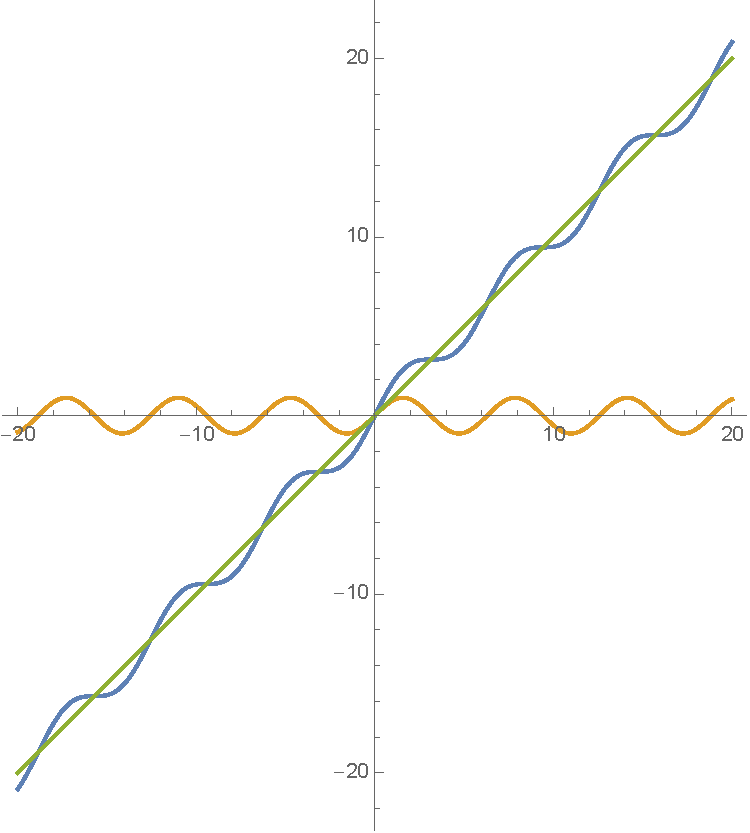
\includegraphics{./images/ch1/xpsinx.pdf}}
\end{center}

[证]:该函数的定义域为$\mathbb{R}$,任取$x_1,x_2\in\mathbb{R}$,则
$$f(x_2)-f(x_1)=(x_2-x_1)+2\sin\df{x_2-x_1}{2}\cos\df{x_2+x_1}{2}.$$

若$x_2-x_1>2\pi$,则由$\sin\df{x_2-x_1}{2}\cos\df{x_2+x_1}{2}\geq -1$,可得
$$f(x_2)-f(x_1)>(x_2-x_1)-2>2\pi-2>0;$$

若$0<x_2-x_1<2\pi$,注意到$|\sin x|<x\;(x>0)$,则有
$$f(x_2)-f(x_1)>(x_2-x_1)-2\left|\sin\df{x_2-x_1}{2}\right|
>(x_2-x_1)-2\df{x_2-x_1}{2}=0.$$

综上所述,对任意$x_2>x_1$,恒有$f(x_2)-f(x_1)>0$,故$f(x)$严格单调递增。
\hfill $\Box$


{\b{\bf 问:}严格单调的函数一定是一一映射,故一定存在反函数。如果反之,
存在反函数的函数一定会严格单调吗?}
\ps{要说明一个命题不成立,只需举出反例即可}

[答]:反之不成立。例如函数
$$f(x)=\left\{\begin{array}{ll}
	x,&0<x<1;\\
	3-x,&1\leq x<2
\end{array}\right.$$
的反函数就是其自身,但在定义域上不是单调的。

进一步思考:以上反例中的函数在每个连续的区间(例如$(0,1)$)上仍然是严格单调的,
这是函数存在反函数的必要条件吗?换句话说,是否存在某个函数存在反函数,
却在任意的区间上都不单调呢?

{\b {\bf 思考:}若对任意$x_1,x_2$,总有
$$[f(x_2)-f(x_1)](x_2-x_1)\leq 0,$$
可以推断$y=f(x)$具有何种性质?}

[答]:$y=f(x)$单调递减。

{\bf 【奇偶性】}

	设函数$f:D\mapsto\mathbb{R}$,{\it 称$f(x)$为偶(奇)函数},是指:
	对任意$x\in D$,有$f(-x)=f(x)\quad(f(-x)=-f(x))$

奇偶性是对称性的一种特例,由奇偶性的定义,很容易得到关于函数对称性的一些定义:

{\bf 例:}试给出如下性质的数学定义
\begin{enumerate}[(1)]
  \setlength{\itemindent}{1cm}
  \item {\b 函数$y=f(x)$的图像关于$x=a$对称
  \dotfill$f(2a-x)=f(x)$}
  \item {\b 函数$y=f(x)$的图像关于点$(x_0,y_0)$对称
  \dotfill $f(2a-x)=2f(a)-f(x)$}
\end{enumerate}

{\b {\bf 思考:}$f(x)=g(a-x),\;(x\in\mathbb{R})$有什么几何意义?

[答]{\it $f(x)$和$g(x)$的图像关于$x=a/2$对称!}}

{\bf 例:}$\sin x=\cos(\pi/2-x)$,
故可知$\sin x$和$\cos x$的图像关于$x=\pi/4$对称。

\begin{thx}
	{\bf 定理:}任意一个定义在对称区间上的函数均可以表示为一个偶函数和一个奇函数的和,即
	$$f(x)=\df{f(x)+f(-x)}{2}+\df{f(x)-f(-x)}{2}.$$
\end{thx}
例如:
$$e^x=\df{e^x+e^{-x}}2+\df{e^x-e^{-x}}2$$

{\bf 【周期性】}

设函数$f:\mathbb{R}\to\mathbb{R}$,
称{\it $f(x)$为周期函数},是指: 存在$T>0$,
使对任意$x\in\mathbb{R}$,有
$f(x+T)=f(x)$。
满足以上性质的最小正数$T$称为$f(x)$的{\it 最小正周期}。
		 
{\bf 注:}若$T$为$f(x)$的一个周期,则任意$n\in\mathbb{Z}$和
任意$x\in\mathbb{R}$,总成立
$$f(x+nT)=f(x).$$

\subsubsection{常用函数}

{\bf 符号函数}

  $${\b \bm{\mathrm{sgn}}\,x =\left\{
	\begin{array}{rl}
	-1,\;&x<0 \\
	0,\;&x=0 \\
	1,\;&x>0
	\end{array}
  \right.}$$
显然,{\b $|x|=x \cdot\mathrm{sgn} x$}
	
{\bf (下)取整函数(阶梯函数)}

  $${\b y=\left[ \,x\, \right]}$$
  $[\,x\,]$表示小于等于$x$的最大整数

{\bf 性质:}
\begin{enumerate}[(1)]
  \setlength{\itemindent}{1cm}
  \item {\b $[x]\leq x<[x]+1$}
  \item {\b $[x+1]=[x]+1$}
\end{enumerate}

{\bf 例:}试给出以下曲线的方程

\begin{center}
	\resizebox{!}{2.5cm}{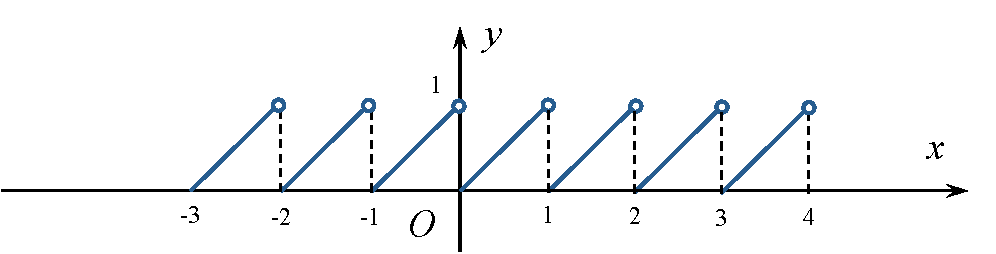
\includegraphics{./images/ch1/f1.pdf}}\quad $y=x-[x]$\\

	\resizebox{!}{2.5cm}{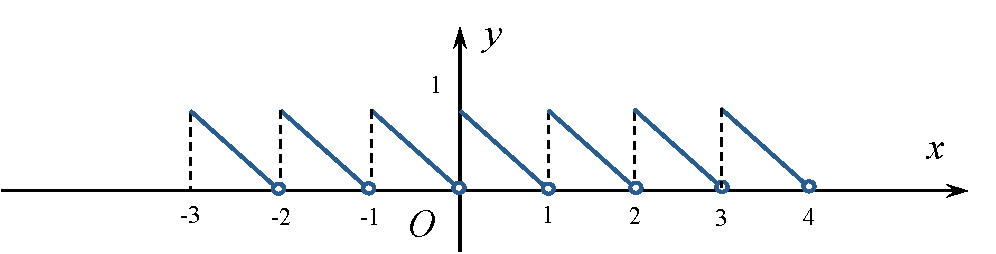
\includegraphics{./images/ch1/f2.pdf}}\quad $y=[x]-x+1$\\

	\resizebox{!}{2.5cm}{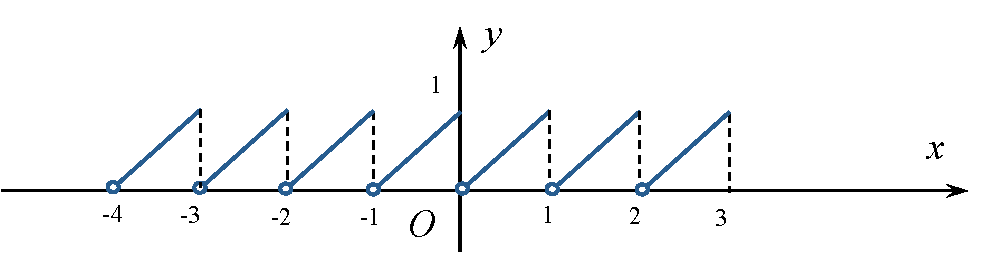
\includegraphics{./images/ch1/f3.pdf}}\quad $y=[-x]+x-1$
\end{center}
	
{\bf 例:}$(-1)^{[x]}$的图像?\quad({\it 方波!})

{\bf 例:}{\it 三角波}
$$y=\left|x-2\left[\df x2\right]\right|
\quad\mbox{或者}\quad
y=\df1{\pi}\arccos(\cos\pi x)$$

\begin{center}
	\resizebox{!}{2cm}{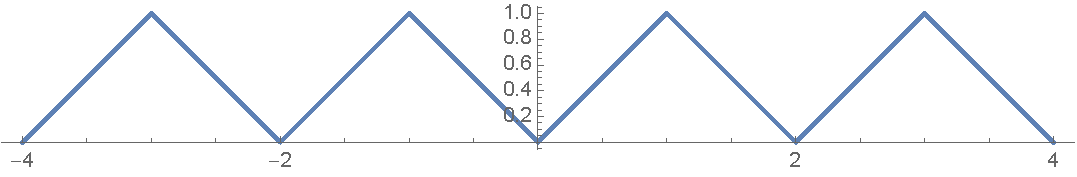
\includegraphics{./images/ch1/trif.pdf}}
\end{center}

{\bf 例:}证明:$f(x)=x-[x]$是以$1$为最小正周期的周期函数。\ps{参见MOOC第四讲}

{\bf Dirichlet函数}
  $${\b \bm{D}(x) =\left\{
  \begin{array}{ll}
  	1,\;& x\in\mathbb{Q} \\
  	0,\;& x\notin\mathbb{Q}
  \end{array}
  \right.}$$
  {\bf 性质:}\ps{在后续章节中加以证明}
  \begin{enumerate}[(1)]
    \setlength{\itemindent}{1cm}
    \item $D(x)$在实数轴上处处无极限
	\item $D(x)$在实数轴上处处不连续
	\item {\it 仅在$x=0$这一点连续的函数:}$y=xD(x)$
	\item {\it 仅在$x=0$这一点可导的函数:}$y=x^2D(x)$
  \end{enumerate}

{\bf Riemann函数} :\ps{这个函数也被称为“直尺函数”,最初由卡尔$\cdot$托梅提出}
设$x\in[0,1]$,
  $$\bm{R}(x) =\left\{
	\begin{array}{ll}
	1,\;&x=0\\
	\displaystyle\frac 1q,\;&x=\displaystyle\frac pq,\,p,q\mbox{互素}\\
	0,\;&x\notin\mathbb{Q}
	\end{array}
  \right. $$
  {\bf 性质:}
  \begin{itemize}
    \item 对任意$x_0\in[0,1]$, $\lim\limits_{x\to x_0}R(x)=0$
    \vspace{1ex}
    \item $R(x)$在{\it 无理数点连续, 有理数点不连续}
    \item $R(x)$是Riemann可积的
  \end{itemize}

{\bf 初等函数}

五类{\bf 基本初等函数}:

\begin{enumerate}
  \setlength{\itemindent}{1cm}
  \item {\it 幂函数:} $y=x^a,\; (a\in\mathbb{R})$
  \ps{只有整数次幂的函数可以手工计算!!!}
  \item {\it 指数函数:} $y=a^x,\; (a>0,a\ne 1)$
  \begin{itemize}
    \item {$y=e^x$}
  \end{itemize}
  \item {\it 对数函数:} $y=\log_ax,\; (a>0,a\ne 1)$
  \begin{itemize}
    \item {$y=\ln x$}
  \end{itemize}
  \item {\it 三角函数:} $\sin x, \,\cos x,\, \tan x, \,\cot
  x,\, \sec x,\, \csc x$
  \item {\it 反三角函数:} $\arcsin x, \,\arccos x, \arctan x,
  \ldots$
\end{enumerate}

{\bf 问:}$\arcsin x$和$\arccos x$的定义域值域有何不同?
\ps{这是中学阶段需要了解的知识,不会的话自己好好补一补}

由常数和基本初等函数经过{\it 有限次}的四则运算和{\it 有限次}的函数复合
步骤所构成并{\it 可用一个式子表示}的函数,称为{\it 初等函数}

{\b 学习要求:熟练掌握五类基本初等函数的定义、图像、基本性质、各种运算公式(例如:
三角函数的和差化积、积化和差、半(倍)角公式、万能公式;反三角函数的定义域、值域、单调性;
一些常用的不等式,如$e^x-1>x>\ln(x+1)\;(x>0)$、平均值不等式、
$\sin x<x<\tan x\;(x>0)$等等。}

{\bf 例:}写出以下两个函数的表达式\ps{MOOC第五讲例1}
$$\arcsin(\sin x),\quad \sin(\arcsin x)$$

{\bf 例:}化简$\tan(\arcsin x),\;x\in(-1,1)$\ps{MOOC第五讲例2}

[解]:注意到
$$\tan x=\df{\sin x}{\cos x}=\df{\sin x}{\sqrt{1-\sin^2x}},$$
故
$$\mbox{原式}=\df x{\sqrt{1-x^2}},\quad x\in(-1,1).$$
\hfill $\Box$

{\bf 思考题:}证明:$\pi=20\arctan\df17+8\arctan\df3{79}$.

[提示]:等式两边都除以$4$,然后取正切,再反复利用
$$\tan(A+B)=\df{\tan A+\tan B}{1-\tan A\tan B}.$$

{\bf ($n$次)多项式(函数)}
\begin{thx}
$$P_n(x)=\sum_{i=0}^na_ix^i,
  \quad (a_i\in\mathbb{R},a_n\ne 0,i=1,2,\ldots,n)$$
  {\bf 性质:}
  \begin{enumerate}[(1)]
    \setlength{\itemindent}{1cm}
    \item { $n$次多项式方程$P_n(x)=0$在$\mathbb{R}$上最多有$n$个根 (包含重根) ,在
    $\mathbb{C}$上有且仅有$n$个根(包含重根)};
    \item 设$x_i\in\mathbb{C}(i=1,2,\ldots,n)$为$P_n(x)=0$的全部根 ,则
    $$P_n(x)=a_n\prod_{i=1}^n(x-x_i)=a_n(x-x_1)(x-x_2)\ldots(x-x_n),$$
    \item 已知$P_n(x)$在$n+1$个点处的值, 可以唯一确定$P_n(x)$。
  \end{enumerate}
\end{thx}

{\bf 有理(分式)函数}
\begin{thx}
$$f(x)=\frac{P(x)}{Q(x)}, \quad\mbox{其中}P(x),Q(x)\mbox{均为多项式函数}$$
\end{thx}
{\bf 注:}{\b 任意有理函数总可以化为一个多项式函数和一个真分式(分子的次数比分母低的有理函数)
的和}
	  
{{\bf 例:}用多项式除法化简以下函数}
$$\frac{x^3+x^2-1}{x-1}=x^2+2x+2+\df{1}{x-1}$$
具体的除法过程如下,类似于小学学习过的竖式除法
\begin{center}
	\polylongdiv{x^3+x^2-1}{x-1}
\end{center}

{\bf 双曲函数}

$$\sinh x =\df{e^x-e^{-x}}{2}, \quad
\cosh x =\df{e^x+e^{-x}}{2}, \quad\tanh x=\df{\sinh
x}{\cosh x}, \ldots$$

{\bf 注:}双曲函数在很多场合也写作$\mathrm{ch}(x)$和$\mathrm{sh}(x)$
\ps{运算规律参见教材}

\bigskip

\begin{ext}
	{\centering\bf 课后作业}
	
	{\b\kaishu 说明:	今后所有的作业必须写在作业本上,作业本第一页背面上贴上一张个人的照片,
	标注专业和籍贯。作业须写明题目所在章节、题号;如非特别说明,	所有题目必须抄题;
	未作或作错的题目讲评后务必及时订正。}
	
	\begin{enumerate}  
	  \item 证明:函数$\mathrm{arsh}\,x=\ln(x+\sqrt{x^2+1})$严格单调递增。
	  \item 证明:函数$y=x\sin x$无界。
	  \item 如左图,将单位圆上的点$Q$映射成数轴上的点$P$的映射称为{\it 球极投影映射},
	  请给出:
	  \begin{enumerate}[(1)]
	    \item $Q$的极角$\theta$与$P$的横坐标$x_P$的对应关系;
	    \item $Q$的坐标$(x_Q,y_Q)$与$P$的坐标$(x_P,y_P)$的对应关系;
	    \item 思考(选作):参考右图,给出将一个单位球面映射为二维平面的
	    {\it 三维球极投影映射},写出具体的对应关系。
	  \end{enumerate}
	\begin{center}
		\resizebox{!}{5cm}{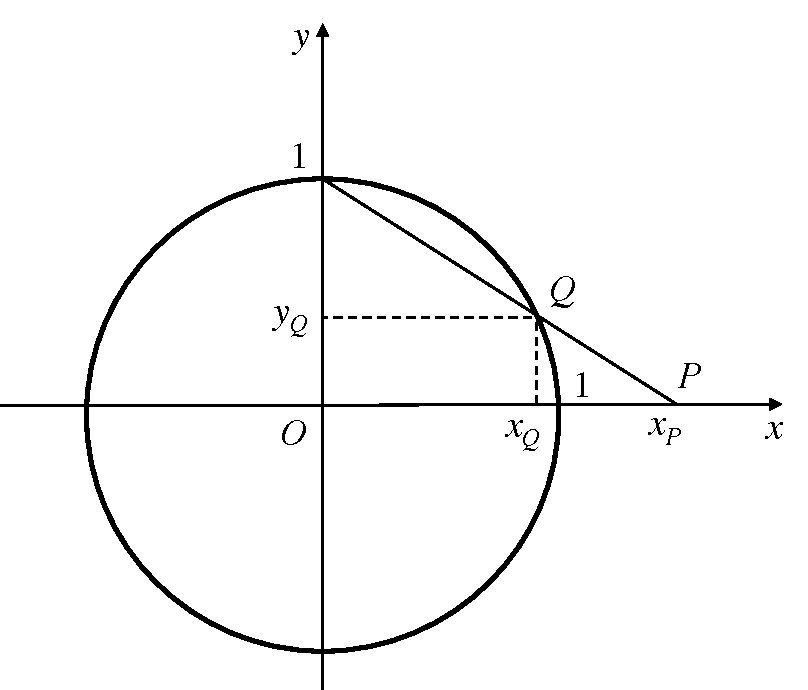
\includegraphics{./images/ch1/answer/sphereline2D.pdf}}\quad
		\resizebox{!}{5cm}{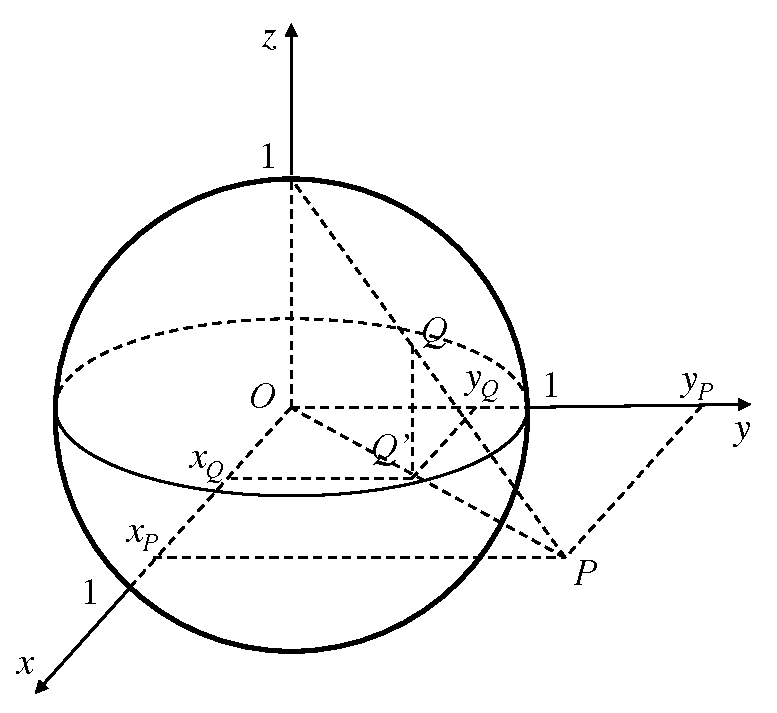
\includegraphics{./images/ch1/answer/sphereline3D.pdf}}
		
		\it \small 第3题图
	\end{center}
	\item (选作)对任意$x_0\in\mathbb{R}$,试给出两个数列$\{x^{(1)}_n\}$和
	$\{x^{(2)}_n\}$,而且分别为有理数列和无理数列,且都以$x_0$为极限。
% 	  \item 习题1-2:5(3,4),7,8
% 	  \item 习题1-3:5(3),6(2),7,8
% 	  \item 习题1-4:7,8
% 	  \item 习题1-5:3
% 	  \item 习题1-6:4(2,3,5)
% 	  \item 习题1-7:4(2),5(3,4)
% 	  \item 习题1-8:4
% 	  \item 习题1-9:2,3(3,5,6),4
% 	  \item 习题1-10:1,5,7
% 	  \item 总习题一:14
	\end{enumerate}
\end{ext}

\section{数列的极限}

极限概念的引入是微积分发展史上具有革命性的一步,为奠定微积分理论“无可非议”的扎实
基础提供了可能。后续我们将要学习的导数、积分、级数等重要概念都是以极限的形式定义的。

数列极限是极限问题中最为简单的一类,也是性质非常典型的一类,可以作为我们后续学习
函数极限的基础。

{\bf 数列:}按一定规律排列的无穷多个(相同或不相同的)数,记作:
\ps{\b 有序性是数列最重要的特征,改变了数列中数的排列顺序将得到不同的数列}
$$a_1,a_2,\ldots,a_n,\ldots\quad\mbox{或者}\quad\{a_n\}.$$
$\{a_n\}$的实质是定义在$\mathbb{N}_+$上的函数,因此也被称为
{\it 整标函数}或{\it 整序函数}。如果在平面直角坐标系内作图,
也可以将其视为一个动点随$n$增大所留下的离散的运动轨迹。

{\bf 思考:}数列与集合有哪些区别?\ps{1、有序-无序;\\ 2、无限-可能有限;\\ 3、可重复-不可重复}

{\bf 例:}数列举例

\begin{enumerate}[(1)]
  \setlength{\itemindent}{1cm}
  \item[(1)] $\left\{\df{n+1}n\right\}:\df 21,\df 32,\df43,\df54,\df65,\ldots$
  \item[(2)] $\left\{\df{(-1)^n}n\right\}:-1,\df12,-\df13,\df14,-\df15,\df16,\ldots$
  \item[(3)] $\{n^2\}:1,4,9,16,25,36,\ldots$
  \item[(4)] $\left\{n^{(-1)^n}\right\}:1,2,\df13,4,\df15,6,\ldots$
\end{enumerate}

\subsection{数列极限的定义}

形象地说,数列$\{a_n\}$的{\it 极限}
\ps{现实生活里的极限更类似于我们所说的上限(确界)和下限(确界),例如:人类速度的极限}
,就是$a_n$的值随$n$的不断增大而趋向的某个确定的值,
当然,对于不同的$\{a_n\}$,这个确定的值不一定都存在!例如:
\begin{itemize}
  \item $\left\{\df1n\right\}$
  的值随着$n$不断增大会越来越趋近于$0$,因此其极限为$0$;
  \item $\{n\}$的取值会越来越大,甚至可以超过任何事先给定给定的值,
  因此也不会趋于任何确定的值,极限不存在;
  \item $\{(-1)^n\}$的取值在$1$和$-1$上反复交替,从整体上看,
  既不能说它趋近与$1$,也不能说它趋近于$-1$,所以极限也不存在。
\end{itemize}

在直观理解的基础上,我们集中来关注一个问题,即:{\it 数学上如何表达这种
趋向某个确定值的特征,或者说,如何给出数列极限的数学定义?}

以下的定义由数学家Weierstrass最终完成(注意,不是发明)\ps{现行的极限符号
$\lim$据说由数学家Hardy(1877-1947)引入,而最初提出通过引入极限来解决
微积分理论不严密问题的人是法国数学家d'Alembert}
,是被数学界最广泛接受的一种极限定义:

\begin{thx}
	对于数列$\{a_n\}$,若存在常数$a$,{\b 对任意$\e>0$(不论它有多小),
	都存在$N\in\mathbb{Z}_+$,使对任意$n>N$,都有
	$$|a_n-a|<\e$$
	成立},
	%\ps{可简写为:$\forall\e>0,\exists N,\forall n>N,|a_n-a|<\e$}
	则称{\bf 数列$\{a_n\}$存在极限(或收敛)},常数$a$称为该数列的极限,记为
	$$\b\lim_{n\to\infty}a_n=a$$
	或%\ps{\b 使用后面一种记号时,必须要写上$(n\to\infty)$}
	$$\b a_n\to a\;(n\to\infty)$$
	若上述常数$a$不存在,则称{\bf 数列$\{a_n\}$不存在极限}(或{\bf 发散})。	
\end{thx}

从几何上看(如下图所示),数列$\{a_n\}$以$a$为极限,意味着随着$n$的增大,$a_n$可以无限地
靠近$a$。为了表达这种“无限靠近”,数学上可以这样来解释:对于以$a$为中心的任意小的邻域$(a-\e,
a+\e)$(图上的蓝色阴影部分),只要把$n$取得充分大($N$的意义就是为了界定这个所谓的充分大
\ps{\b 显然,$\e$取得越小通常意味着$N$要取得越大,但必须注意的是$N$和$\e$
之间并不是简单的函数对应关系,因为如果某个$N$可以满足命题要求,
则$N$加任意的正常数显然也满足}
),则$a_n$都将落在$(a-\e,a+\e)$之内
\ps{\b 除了有限多个$a_n$外(准确地说是除了至多$\{a_n\}$的前$N$项外)}
。

\begin{center}
	\resizebox{!}{3cm}{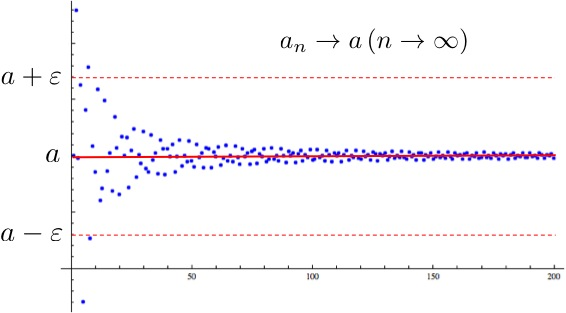
\includegraphics{./images/ch2/lim-en/en1.jpg}}\quad
	\resizebox{!}{3cm}{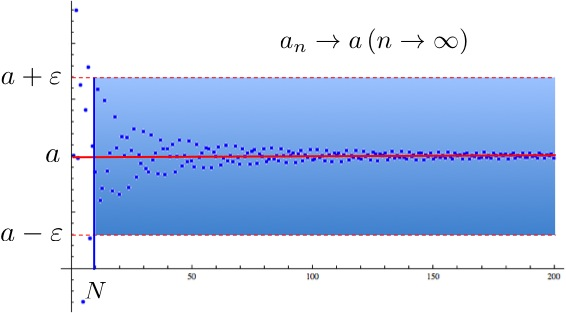
\includegraphics{./images/ch2/lim-en/en2.jpg}}
	
	\resizebox{!}{3cm}{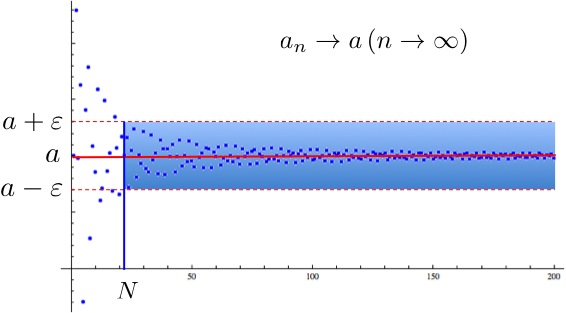
\includegraphics{./images/ch2/lim-en/en3.jpg}}\quad
	\resizebox{!}{3cm}{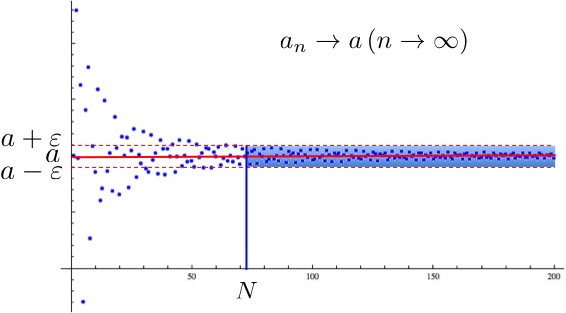
\includegraphics{./images/ch2/lim-en/en4.jpg}}
% 	
% 	\resizebox{!}{3cm}{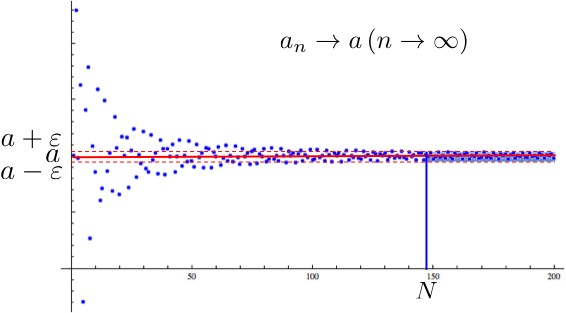
\includegraphics{./images/ch2/lim-en/en5.jpg}}
\end{center}

\begin{shaded}
	关于极限的定义,历史上曾经有过很长时间的讨论,当时的许多数学家都尝试
	过给出一个“合适”的极限定义,例如:Cauchy是这样描述极限的:
	
	{\kaishu
		当属于一个变量的相继值无限地趋近某个固定值时,如果以这样一种方式告终,
		变量值同固定值之差小到我们希望当任意小,那么这个固定值就成为其他所有值的极限。
	}
	
	这个定义中所描述的“趋近”这个行动,很难说是一种令人满意的表达方式。趋近是指
	一种实际的动作吗?如果是,是否意味着我们在讨论极限时,必须把时间和空间的概念
	包含在内?此外,什么才是这个过程的“告终”?
	
	相对而言,Weierstrass的极限定义里,没有任何动作,不涉及任何时间,完全
	是一个“{\it 静态的而非动态的定义}”,同时又是一个“{\it 代数的而非几何的定义}”。
	定义的核心是一个关于不等式的断言(命题)。最重要的是,利用它能够很容易地
	证明各种关于极限的定理,例如“和的极限等于极限的和”、“极限的保号性”。
	至此,对于类似的定理终于可以像Euclid的几何命题一样完全地严格化了。
	这是微积分发展历史上一个巨大的进步。
	
	Weierstrass被称为“{\it 现代分析学之父}”,《微积分的历程》一书这样评价他:
	{\kaishu
		19世纪,数学家们将微积分的严格性提高到一个新的水平。然而,按照我们今天的标准,
		这些成就并不是无可挑剔的。当你拜读那个时期的数学文献时,犹如聆听音乐大师肖邦
		在一架三两琴键失调的钢琴上演奏乐章,固然能够怡然自得地鉴赏音乐的神韵,不过
		间或也会听到些许畸变之音。只有在微积分中消除不精确的最后痕迹,分析论证变成对于
		一切实用目的都是无可置疑的时候,数学的新纪元才能到来,Weierstrass正是
		实现这个最后转变的最大功臣。 
		
		\ldots\ldots
		
		Weierstrass学派通过Weierstrass本人或者他的门生们发表的研究成果,对分析学
		赋予逻辑上的一种无与伦比的精确性。他矫正了许多难以捉摸的错误概念,证明了大量
		重要的定理,并且构造出一个令数学家们惊叹不已的处处连续而又不可微的函数的反例。
	}
	
	Weierstrass同时还是一名出色的数学教育家,Hiene(1821-1881)和Cantor都是他的门生。
\end{shaded}
	
前述定义更为简洁的写法:
\ps{\it\b 这种纯符号的表述方式固然简洁,但要正确掌握,
必须首先对更完整的文字表述有准确的理解,否则不建议随意使用}
$${\b \forall\e>0,\exists N\in\mathbb{Z}_+,\forall n>N,|a_n-a|<\e}\eqno{(1)}$$

{\bf 讨论:}以下说法和$(1)$等价的是:

\begin{enumerate}
  \setlength{\itemindent}{1cm}
%   \item[(2)] $\forall\e>0$,$\exists N>0$,$\forall
%   n>N$,$|a_n-a|<\e$ \hfill{$\surd$}\\
%   \hfill(直接写$\exists N$即可)
  \item[(2)] $\forall\e>0$,$\exists N$,$\forall
  n>N$,$|a_n-a|\leq\e$ \hfill{$\surd$} 
  
  \quad [提示]:只要强调$n>N$为正整数即可,根据需要$N$总是可以取得更大,
  无所谓是不是正整数。
  \item[(3)] $\exists N\in\mathbb{Z}_+$,$\forall\e>0$,$\forall
  n>N$,$|a_n-a|<\e$ \hfill{$\times$}
  
  \quad [提示]:(3)可以推出(1),但反之不然。事实上,由(3)可以推出,
  $\{a_n\}$仅有有限项的值不等于$a$,但显然不是所有收敛的数列都有此
  性质,例如$\{1/n\}$
  \item[(4)] $\forall\e>0$,仅有有限多个$n$,使得$|a_n-a|\geq\e$
  \hfill{$\surd$}
  
  \quad [提示]:由(4),仅有有限多个$a_n$不满足$|a_n-a|<\e$,则我们总可以取
  其中下标最大的下标作为$N$,则当$n>N$时,总有$|a_n-a|<\e$,即(1)成立;反之,由
  (1),最多有不超过$N$个$a_n$不满足$|a_n-a|<\e$,故(4)成立。
  
  \item[(5)] $\forall\e>0$,总有无穷多个$n$,使得$|a_n-a|<\e$
  \hfill{$\times$} 
  
  \quad [提示]:考虑反例:$a_n=(-1)^n$,取$a=1$。
  \item[(6)] $\forall\e>0$,要使$|a_n-a|<\e$,只须$n$充分大 \hfill{$\surd$}
  
  \quad [提示]:语序有变化,但逻辑关系和含义并未发生改变。
  \item[(7)] $\forall\e>0,\exists N\in\mathbb{Z}_+,\forall
  n>N,|a_n-a|<2\e$\hfill{$\surd$}
  
  {\quad\b\kaishu [注]:由于$\e$是任意的,$2\e$和$\e$的取值范围并没有区别,都是
  $(0,+\infty)$!事实上,在用定义证明极限时,完全可以使用$C\e$,
  其中$C\in\mathbb{R}$为给定的常数,这是数列极限最常用的一种等价定义。}
\end{enumerate}

{\bf 例:}证明:
$$\limn(-1)^n\df1{n^2}=0$$

[证]:对任意$\e>0$,{\b 令$N=\left[1/\sqrt{\e}\right]+1$}
\ps{不要忘记:\b $[x]\leq x<[x]+1$}
,则对任意$n>N$,有
$$\left|(-1)^n\df1{n^2}-0\right|=\df1{n^2}<\df1{N^2}
<\df1{(\sqrt{\e})^2}=\e,$$
由极限的定义,即证。\ps{\b 用定义证明数列极限,说明$N$的存在性是关键,为此主要有两种方式:\\
1、直接给出$N$的取值,例如$N=1/\e$\\
2、利用已知极限间接说明$N$存在,如$N=N_1$}
\hfill $\Box$

{\bf 例:}证明:
$$\limn\left(\df n{n+1}\right)^2=1$$

[证]:对任意$\e>0$,{\b 令$N=\left[2/\e\right]+1$},则对任意$n>N$,有
$$\left|\left(\df
n{n+1}\right)^2-1\right|=\df{2n+1}{(n+1)^2}<\df{2(n+1)}{(n+1)^2}
<\df2{n+1}<\df2n<\df2N<\e,$$
由极限的定义,即证。\hfill $\Box$

{\bf 例:}证明:若$\limn a_n=a$,则$\limn|a_n|=|a|$

[证]:对任意$\e>0$,由$\limn a_n=a$可知,存在$N_1\in\mathbb{Z}_+$,
对任意$n>N_1$,有
$$|a_n-a|<\e.$$
于是{\b 令$N=N_1$},则对任意$n>N$,有\ps{\b 利用$N_1$的存在性间接说明了$N$的存在性}
$$||a_n|-|a||\leq|a_n-a|<\e,$$
由极限的定义,即证。\hfill $\Box$

{\bf 课堂练习:}证明:若$|q|<1$,则$\{q^n\}$收敛。

[提示]:令$N=\left[\log_{|q|}\e\right]+1$

% {\bf 思考:}已知$|q|>1$时,$\{q^n\}$发散,请问该如何证明?
% 
% {\bf 注:}利用有界性,也可以证明发散。

\begin{shaded}
	{\bf 【极限定义的反面说法】}
	
	参照上一节对反面说法的介绍,由数列$\{a_n\}$以$a$为极限的定义:
	$$\limn a_n= a\quad\Leftrightarrow\quad\forall\e_0>0,
	\exists N\in\mathbb{Z}_+,\forall n>N,|a_n-a|<\e_0$$
	可以写出{\it 数列$\{a_n\}$不以$a$为极限}的定义:
	\begin{tcolorbox}
		$$\limn a_n\neq a\quad\Leftrightarrow\quad\exists\e_0>0,
		\forall N\in\mathbb{Z}_+,\exists n_0>N,|a_{n_0}-a|\geq\e_0$$
	\end{tcolorbox}
	
	下面用这个定义来证明几个例子:
	
	{\bf 例:}证明:$\limn\df 1n\neq 1$.
	
	[证]:取$\e=\df12$,对任意$N\in\mathbb{Z}_+$,令$n_0=\max\{3,N+1\}>N$,
	从而
	$$\left|\df1{n_0}-1\right|=1-\df1{n_0}\geq 1-\df13=\df23>\e,$$
	由极限的反面定义,即证。\hfill $\Box$
	
	{\bf 例:}证明$\{(-1)^n\}$发散。
	
	[证]:任取$a\in\mathbb{R}$,只需证明$\limn(-1)^n\ne a$。以下不妨设$a>0$。
	
	取$\e=1$,对任意$N\in\mathbb{Z}_+$,令$n_0=\max\{2[N]+1,1\}>N$,则
	$$\left|(-1)^{n_0}-a\right|=|-1-a|=a+1>\e,$$
	由极限的反面定义,即证。\hfill $\Box$
	
	相对于使用的反证法,用反面定义证明极限不存在,形式上更简洁,但
	却不是特别直观和容易理解。
	
	需要提醒的是,数列不以某个值为极限和数列发散是两个不同的概念,后者意味着
	数列不以任何的值为极限。
	
	{\bf 思考:}数列发散可能有哪些不同的情形?\hfill({\it 趋向无穷,或反复振荡不收敛})
\end{shaded}

\subsection{数列极限的性质}

以下三个性质的证明,可以作为用极限定义证明命题的典型例子,应重点理解、掌握。

\begin{thx}
	{\bf 唯一性:}数列极限若存在,必唯一。
\end{thx}

可以说,是唯一性的要求决定了当前的极限定义。从这个意义上说,目前使用的极限定义其实也是一种约定。
%“记录重大技术突破的技术发展史其实就是一部人类社会发展的技术选择史”

\begin{center}
	\resizebox{!}{4cm}{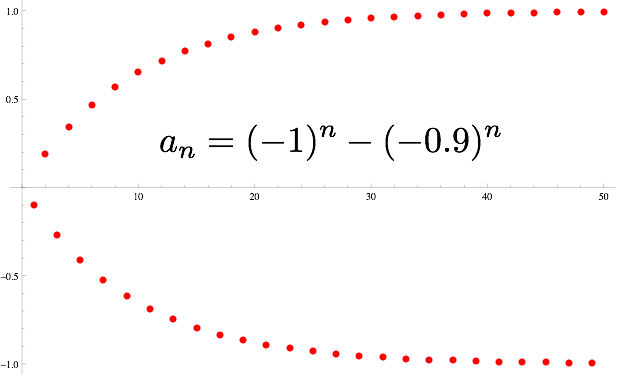
\includegraphics{./images/ch2/1-0.9n.jpg}}
	
	一个不收敛的数列
\end{center}

下面的证明需要用到如下的命题:设$a,b\in\mathbb{R}$,若对任意$\e>0$,
有$|a-b|<\e$,当且仅当$a=b$
\ps{\b 两个确定的数如果可以无限靠近(小于任意给定的距离),则意味着它们相等。}

[证]:设$a,b$均为数列$\{a_n\}$的极限。

对任意$\e>0$,由$\limn a_n=a$,存在$N_1\in\mathbb{Z}_+$,对任意$n>N_1$,有$|a_n-a|<\e$;

同理,由$\limn a_n=b$,存在$N_2\in\mathbb{Z}_+$,对任意$n>N_2$,有$|a_n-b|<\e$。

令{\b $N=\max\{N_1,N_2\}$},则当$n>N$时,有
$${\b |a-b|\leq|a_n-a|+|a_n-b|<2\e},$$
由此可知,必有$a=b$,即证。\hfill $\Box$

\begin{thx}
	{\bf 有界性:}数列$\{a_n\}$若收敛,则{\it $\{a_n\}$有界},即:存在$M>0$,对任意
	$n\in\mathbb{Z}_+$,恒有$|a_n|\leq M$。	
\end{thx}

\begin{center}
	\resizebox{!}{4cm}{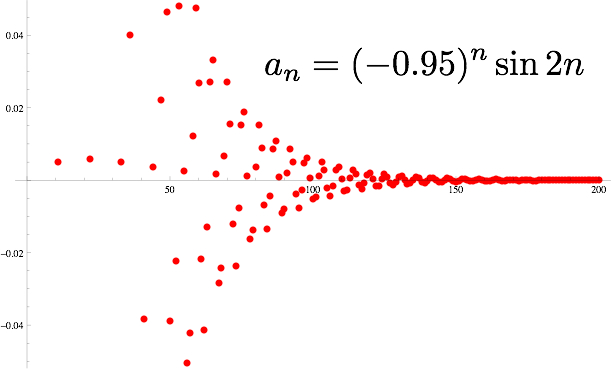
\includegraphics{./images/ch2/sin2nn.jpg}}
	
	一个收敛的数列
\end{center}

思路:{\b 利用$\e$的特定取值“控制”无穷的部分,剩余的有限多个数构成的集合自然是有界的}

[证]:记$\limn a_n=a$。由极限的定义,对{\b$\e=1$},存在$N\in\mathbb{Z}_+$,
对任意$n>N$,有
$$|a_n-a|<\e=1\quad\Rightarrow\quad |a_n|<|a|+1.$$
记{\b$M=\max\{|a|+1,|a_1|,|a_2|,\ldots,|a_{[N]+1}|\}$},则对
任意$n\in\mathbb{Z}_+$,均有
$$|a_n|\leq M,$$
即证。\hfill $\Box$

该性质的一个显然的推论是:{\b 如果数列无界,则必发散。}

{\bf 例:}讨论$\{\sqrt[n]{n!}\}$的敛散性。

思路:对任意$M>0$,当$n$充分大时,总有$n!>M^n$,故$\{\sqrt[n]{n!}\}$无界,
从而发散。

[证]:对任意$M>0$,令$N=[2M]+1$,则当$n>N$时,总有$n>2M$。此时
$$\df{n!}{M^n}=\df{N!}{M^N}\cdot\df{N+1}{M}
\cdot\df{N+2}{M}\ldots\df{n}{M}<\df{N!}{M^N}\cdot2^{n-N+1}.$$
注意到$\df{N!}{M^N}$为有限值,而$2^{n-N+1}$随着$n$的增大趋于正无穷,
故当$n$充分大时,必有
$$\df{n!}{M^n}=\df{N!}{M^N}\cdot2^{n-N+1}>1,$$
从而$\sqrt[n]{n!}>M$,也即$\{\sqrt[n]{n!}\}$无界,故发散。\hfill $\Box$

\begin{thx}
	{\bf 保号性:}设$\lim\limits_{n\to\infty}a_n=a>0$,则存在$N$,
	对任意$n>N$,$a_n>0$	
\end{thx}

[证]:由$\lim\limits_{n\to\infty}a_n=a>0$,对$\e=a/2$,存在
$N$,对任意$n>N$,
$$|a_n-a|<\e=a/2\quad\Rightarrow\quad \df32a>a_n>a/2>0,$$
即证。\hfill $\Box$
		
保号性有几种不同的表达形式(几个推论):
\begin{thx}
	\begin{enumerate}
% 	  \setlength{\itemindent}{1cm}
	  \item 对任意$n\in\mathbb{N}$,$a_n\geq
	  0$, $\lim\limits_{n\to\infty}a_n=a$, 则$a\geq 0$
	%    \ps{\b 保号性可以理解为极限运算保持不等号的方向不变,即:
	%    若$\{a_n\}$收敛,则由$a_n\geq 0$可推出$\limn a_n\geq0$} 
	  \item 设$\lim\limits_{n\to\infty}a_n=a\ne
	  0$, 则$\exists N$,当$n>N$时,$|a_n|>|a|/2$
	  \item  设$\lim\limits_{n\to\infty}a_n=a$, 且最多有有限
	  个$a_n$小于零, 则$a\geq 0$
	\end{enumerate}	
\end{thx}


{\bf 注:}{\b 保号性的实质,是{\it 极限运算保持不等号的方向
\ps{但严格大(小)于可能变成大(小)于等于}不变},
若已知$\limn a_n=a,\limn b_n=b$,则
$$a_n\geq b_n\,(n\in\mathbb{Z}_+)\quad\Rightarrow
\quad\limn a_n\geq\limn b_n$$
}

\begin{thx}
	{\bf 收敛数列与其子数列的关系:}数列$\{a_n\}$收敛,当且仅当它的所有
	子列均收敛到相同的极限。	
\end{thx}

{\it 子数列:}从原数列中按一定顺序选取数,所构成的一个新的数列,通常记为
$\{a_{n_k}\}$,其中$\{n_k\}$是一个严格单调递增的正整数列。显然,
对{\b 任意$k\in\mathbb{Z}_+$,$n_k\geq k$。}

数列$\{a_n\}$的{\it 奇子列}和{\it 偶子列}可记为$\{a_{2k}\}$、$\{a_{2k-1}\}$,
有时也直接写为$\{a_{2n}\}$、$\{a_{2n-1}\}$。

{\it 子数列$\{a_{n_k}\}$以$a$为极限},
也即:对任意$\e>0$,存在$K\in\mathbb{Z}_+$,使对任意$k>K$,总有
$$|a_{n_l}-a|<\e.$$
记为\ps{强调$k$变化而不是$n$变化,事实上$n_k$可以视为整序函数的复合函数中的中间变量}
$$\b\lim\limits_{k\to\infty}a_{n_k}=a,\quad 
\mbox{或}\quad a_{n_k}\to a\;{(k\to\infty)}$$

下面证明上述性质:

[证]:充分性是显然的,因为$\{a_n\}$可以看成是自身的一个子列。

下面证明必要性。设$\limn a_n=a$,则对任意$\e>0$,存在$N\in\mathbb{Z}_+$,
使对任意$n>N$,有$|a_n-a|<\e$。

设$\{a_{n_k}\}$为$\{a_n\}$的任一子列。令$K=N$,则由$\{n_k\}$严格单调递增,
可知对任意$k>K$,都有$n_k>n_K\geq K=N$,从而 
$$|a_{n_k}-a|<\e.$$
也即$\lim\limits_{k\to\infty}a_{n_k}=a$。因为$\{a_{n_k}\}$是任意的,即证。
\hfill $\Box$

% 该性质的另一种表述方法:
% $$\limn a_n=a\quad\Leftrightarrow\quad
% \mbox{对任意严格单调递增的正整数数列}\{n_k\},
% \lim_{k\to\infty}a_{n_k}=a.$$

这个性质的一个明显用途,是判定一些数列的发散。

{\bf 例:}证明数列$\{(-1)^n\}$发散。

[证]:取该数列的偶子列和奇子列,分别即为$\{a_{2k}\}$和$\{a_{2k-1}\}$。显然,
对任意$k\in\mathbb{Z}_+$,都有
$$a_{2k}\equiv 1,\quad a_{2k-1}\equiv -1,$$
因此
$$\lim\limits_{k\to\infty}a_{2k}=1,\quad
\lim\limits_{k\to\infty}a_{2k-1}=-1.$$
由二者极限不相等可知原级数发散,即证。\hfill $\Box$

这种方法证明发散,比前面使用数列收敛的反面定义要更加简洁,也更加直观。

{\bf 例:}\ps{KD教材2.2.2节-例4}
证明数列$\left\{n^{(-1)^n}\right\}$发散。

[提示]:原数列存在发散子列$\left\{(2n)^{(-1)^{2n}}\right\}=\{2n\}$。

{\bf 例:}证明$\left\{\left(1+\df1{\sqrt n}\right)\sin\df{\pi\sqrt n}2\right\}$
发散。

[提示]:取$n_k=k^2$。 

\begin{shaded}
	{\bf 例:}证明:$\{\sin n\}$发散。
	
	[证一]:用反证法。设有$\limn\sin n=a$,则
	$$\limn[\sin(n+2)-\sin n]=0.$$
	进而由
	$$\sin(n+2)-\sin n=2\sin 1\cos(n+1),$$
	可得$\limn\cos(n+1)=0$。又
	$$\cos(n+1)=\cos n\cos 1-\sin n\sin 1,$$
	可得$\limn\sin n=0$。如此就有
	$$\limn\sin n=\limn\cos n=0,$$
	显然与$\sin^2n+\cos^2n=1$矛盾。\hfill $\Box$
	
	[证二]:注意到当$x\in[2k\pi+\pi/4,2k\pi+3\pi/4]\,(k\in\mathbb{N})$时,总有
	$$\sin x>\sqrt2/2.$$
	由于此类区间的长度均超过$1$,故其中必包含至少一个自然数。于是对每个$k\in\mathbb{N}$,
	可取自然数$n^{(1)}_k\in[2k\pi+\pi/4,2k\pi+3\pi/4]$,显然$\{\sin{n^{(1)}_k}\}$构成了$\{\sin
	n\}$的一个子列。
	
	若$\{\sin n\}$收敛,则$\{\sin{n^{(1)}_k}\}$也收敛,且与之极限相同。由极限的保号性,
	可知$\{\sin{n^{(1)}_k}\}$的极限不小于$\sqrt2/2$,从而$\{\sin
	n\}$的极限应大于等于$\sqrt2/2$。
	
	同理,利用区间$[2k\pi+5\pi/4,2k\pi+7\pi/4]\,(k\in\mathbb{N})$,可构造$\{\sin
	n\}$的另一个子列 $\{\sin{n^{(2)}_k}\}$。若$\{\sin n\}$收敛,同样利用保号性可证明其极限应小于等于$-\sqrt2/2$。
	
	以上两方面的结论矛盾,故假设错误,即证。\hfill $\Box$
\end{shaded}

该性质类似的一个结论如下:
\begin{thx}
	{\bf 拉链定理}:若某个数列的奇子列和偶子列收敛到相同的极限,
	则该数列收敛。
\end{thx}

请自行尝试证明该定理。注意,这个定理并不是子数列性质的简单推论。
此外,还请想一想,这个定理可以进一步推广吗?

{\bf 注:}更一般性的推广:如果选择的多个子列按顺序合并起来能够完全覆盖原数列,
或最多不能覆盖原数列中有限多个数,且这些子列均收敛于相同的极限,则原数列收敛。
例如:{\it 若子数列$\{a_{3n}\},\{a_{3n-1},\{a_{3n-2}\}\}$都收敛于$a$,
则$\{a_{n}\}$收敛于$a$。}

\begin{shaded}

{\bf 思考题:}证明:

\begin{tcolorbox}
	{\bf Cauchy命题}:若$\limn a_n=a$,则$\limn\df{a_1+a_2+\ldots+a_n}n=a$。
\end{tcolorbox}

[证]:对任意$\e>0$,由$\limn a_n=a$,存在$N_1$,对任意$n>N_1$,总有
$$|a_n-a|<\e.$$
记
$$M_{N_1}=|(a_1-a)+(a_2-a)+\ldots+(a_{N_1}-a)|,$$
显然$M_{N_1}$的值只与$N_1$有关,而与$n$无关,故令$N_2=\df{M_{N_1}}{\e}$,
则对任意$n>N_2$,总有
$$\df{M_{N_1}}{n}<\e.$$

至此,令$N=\max\{N_1,N_2\}$,则对任意$n>N$,均有
\begin{align*}
	&\left|\df{a_1+a_2+\ldots+a_n}n-a\right|\\
	&=\df1n|(a_1-a)+(a_2-a)+\ldots+(a_n-a)|\\
	&\leq\df1n\left[M_{N_1}
	+|(a_{{N_1}+1}-a)+(a_{{N_1}+2}-a)+\ldots+(a_n-a)|\right]\\
	&<\e+\df1n\left[|a_{{N_1}+1}-a|+|a_{{N_1}+2}-a|
	+\ldots+|a_n-a|\right]\\
	&<\e+\df1n(n-{N_1})\e<2\e,
\end{align*}
由数列极限的定义,即证。\hfill$\Box$

这个结论也称为Cauchy{\it 极限},有着非常重要的应用,例如,今后我们会学习
下面的极限$\limn\sqrt[n]a=1,\,(a>0)$,于是立即可以得到
$$\limn\df1n(a+\sqrt[2]a+\sqrt[3]a+\ldots+\sqrt[n]a)=1.$$

此外,我们今后还会学习到极限运算和初等函数运算可以交换次序,进而可以证明如下的命题:

{\bf 例:}证明:
\begin{tcolorbox}
	设$a_n$均大于零,且$\limn\df{a_{n+1}}{a_n}=q$,则
	$\limn\sqrt[n]{a_n}=q$。	
\end{tcolorbox}


[证]:记$b_1=a_1$,$b_n=\df{a_n}{a_{n-1}}\;(n>1)$,则
% $$a_n=\df{a_n}{a_{n-1}}\cdot\df{a_{n-1}}{a_{n-2}}
% \cdots\df{a_2}{a_1}\cdot a_1$$
$$a_n=b_n\cdot b_{n-1}\cdots b_1,$$
进而
$$\ln a_n=\ln b_n+\ln b_{n-1}+\ldots+\ln b_1,$$
已知$\limn b_n=q$,根据初等函数的性质,可得$\limn\ln b_n=\ln q$,
于是由Cauchy极限,
$$\limn\ln \sqrt[n]{a_n}=\limn\df1n\ln a_n=\limn\df1n\left(
\ln b_n+\ln b_{n-1}+\ldots+\ln b_1\right)=\ln q,$$
进而可得$\limn\sqrt[n]{a_n}=q$。\hfill$\Box$

有了这个定理,我们很容易得到下面的结论:

\begin{tcolorbox}
	若$\limn a_n=a\geq 0$,则
	$$\limn\sqrt[n]{a_1a_2\ldots a_n}=a.$$
\end{tcolorbox}

参考前述的Cauchy命题证明方法,可以求解如下的例子:

{\bf 例:} 已知$\limn a_n=A$且$0<\lambda<1$,求
$$\limn(a_n+\lambda a_{n-1}+\lambda^2a_{n-2}
+\ldots+\lambda^na_0).$$

[解]:
\begin{align*}
	\mbox{原式}&=\limn[(a_n-A)+\lambda(a_{n-1}-A)+\ldots
	+\lambda^n(a_0-A)+A(1+\lambda+\lambda^2+\ldots+\lambda^n)]\\
	&=\limn[(a_n-A)+\lambda(a_{n-1}-A)+\ldots
	+\lambda^n(a_0-A)]
	+A\limn(1+\lambda+\lambda^2+\ldots+\lambda^n)\\
	&=\limn[(a_n-A)+\lambda(a_{n-1}-A)+\ldots
	+\lambda^n(a_0-A)]+\df A{1-\lambda}.
\end{align*} 
由$\limn a_n=A$,可知存在$N_1$,对任意$n>N_1$,有$|a_n-A|<\e.$
从而
\begin{align*}
	&|(a_n-A)+\lambda(a_{n-1}-A)+\ldots+\lambda^n(a_0-A)|\\
	&\leq|a_n-A|+\lambda|a_{n-1}-A|+\ldots+\lambda^{n-N_1-1}|a_{N_1+1}-A|\\
	&\quad+\lambda^{n-N_1}|a_{N_1}-A|+\ldots+\lambda^{n}|a_0-A|\\
	&<\e(1+\lambda+\ldots+\lambda^{n-N_1-1})
	+\lambda^{n-N_1}|a_{N_1}-A|+\ldots+\lambda^{n}|a_0-A|\\
	&<\df{\e}{1-\lambda}+\lambda^{n-N_1}(|a_{N_1}-A|+\ldots+|a_0-A|).
\end{align*}
注意到$M_{N_1}=|a_{N_1}-A|+\ldots+|a_0-A|$与$n$无关,故令
$n>N_2=N_1+\log_{\lambda}\df{\e}{M_{N_1}}$,则有
$$\lambda^{n-N_1}(|a_{N_1}-A|+\ldots+|a_0-A|)<\e.$$
综上当$n>N_2$时,必有
$$|(a_n-A)+\lambda(a_{n-1}-A)+\ldots+\lambda^n(a_0-A)|
<\left(\df1{1-\lambda}+1\right)\e,$$
于是由极限的定义,
$$\limn[(a_n-A)+\lambda(a_{n-1}-A)+\ldots+\lambda^n(a_0-A)]=0.$$
故所求结果为$\df A{1-\lambda}$。\hfill$\Box$

\end{shaded}

\begin{ext}
	{\centering\bf 课后作业}
	
	\begin{enumerate}  
	  \item 用定义证明如下极限:
	  \begin{enumerate}[(1)]
	    \item $\limn\df{\sqrt{n^2+a^2}}n=1$;
	    \item $\limn0.\underbrace{999\ldots9}_{n\mbox{\footnotesize 个}}=1$;
	    \item $\limn(\sqrt[3]{n+1}-\sqrt[3]n)=0$;
	    \item $\limn\df{n^2-n-1}{2n^2+2n-4}=\df12$。
	  \end{enumerate}
	  \item 设数列$\{a_n\}$有界,$\limn b_n=0$,证明:$\limn a_nb_n=0$。
	  \item 设$\limn a_n=a\ne 0$,证明:存在$N\in\mathbb{Z}^+$,对任意
	  $n>N$,有$|a_n|>|a|/2$。
	\end{enumerate}
\end{ext}

\section{函数的极限}

\subsection{函数极限的定义}

函数极限是我们后续定义导数、积分的概念的基础。从形式上看,可以将它视为数列极限的推广,
但从直观意义上看,二者存在很大的不同。

不同于数列极限只有单一的$n\to\infty$一种(自变量的变化)趋势,
函数极限共有{\it 六种可能的(自变量变化)趋势},分为两大类:

\begin{itemize}
  \setlength{\itemindent}{1cm}
  \item {\it 自变量趋于无穷}
  $$\b x\to\infty,\quad x\to+\infty,\quad x\to-\infty$$
  \item {\it 自变量趋于有限值}
  $$\b x\to x_0,\quad x\to x_0^+,\quad x\to x_0^-$$
\end{itemize}

{\bf 思考:} $\limn f(n)=A\Leftrightarrow\limx{+\infty}f(x)=A$成立吗?

答:显然,{\b$\limx{+\infty}f(x)=A$可以推出$\limn f(n)=A$,但反之不然},
\ps{事实上,$f(n)$的值域是$f(x)$值域的子集}

例如:$y=\sin\pi x$当$x\to+\infty$时不收敛,但$\limn\sin n\pi=0$。

\begin{thx}
	{\bf $x$趋于无穷时的函数极限}
	\begin{enumerate}%[(1)]
	  \item $\limx{+\infty}f(x)=A\quad\Leftrightarrow\quad
	  \forall \e>0,{\b\exists X>0,\forall x>X},|f(x)-A|<\e$
	  \item $\limx{-\infty}f(x)=A\quad\Leftrightarrow\quad
	  \forall \e>0,{\b\exists X<0,\forall x<X},|f(x)-A|<\e$
	  \item $\limx{\infty}f(x)=A\quad\Leftrightarrow\quad
	  \forall \e>0,{\b\exists X>0,\forall |x|>X},|f(x)-A|<\e$
	\end{enumerate}
\end{thx}


{\bf 注:}和数列极限类似,在函数极限的定义中,最后不等式右端的$\e$可以改写为$C\e$,
其中$C>0$为常数,所得命题与原定义等价。

{\bf 例:}证明$\limx{+\infty}\df1{\sqrt x}=0$.

[证]:对任意$\e>0$,取$X=\df1{\e^2}$,则对任意的$x>X$,都有
$$\left|\df1{\sqrt x}-0\right|=\df1{\sqrt x}<\df1{1/\e}=\e,$$
由函数极限的定义,即证。\hfill $\Box$

{\b 趋于无穷的函数极限存在,意味着函数存在{\it 水平渐近线}},需要注意的是,
水平渐近线最多可以有两条,例如:

% \begin{center}
% 	\resizebox{!}{4cm}{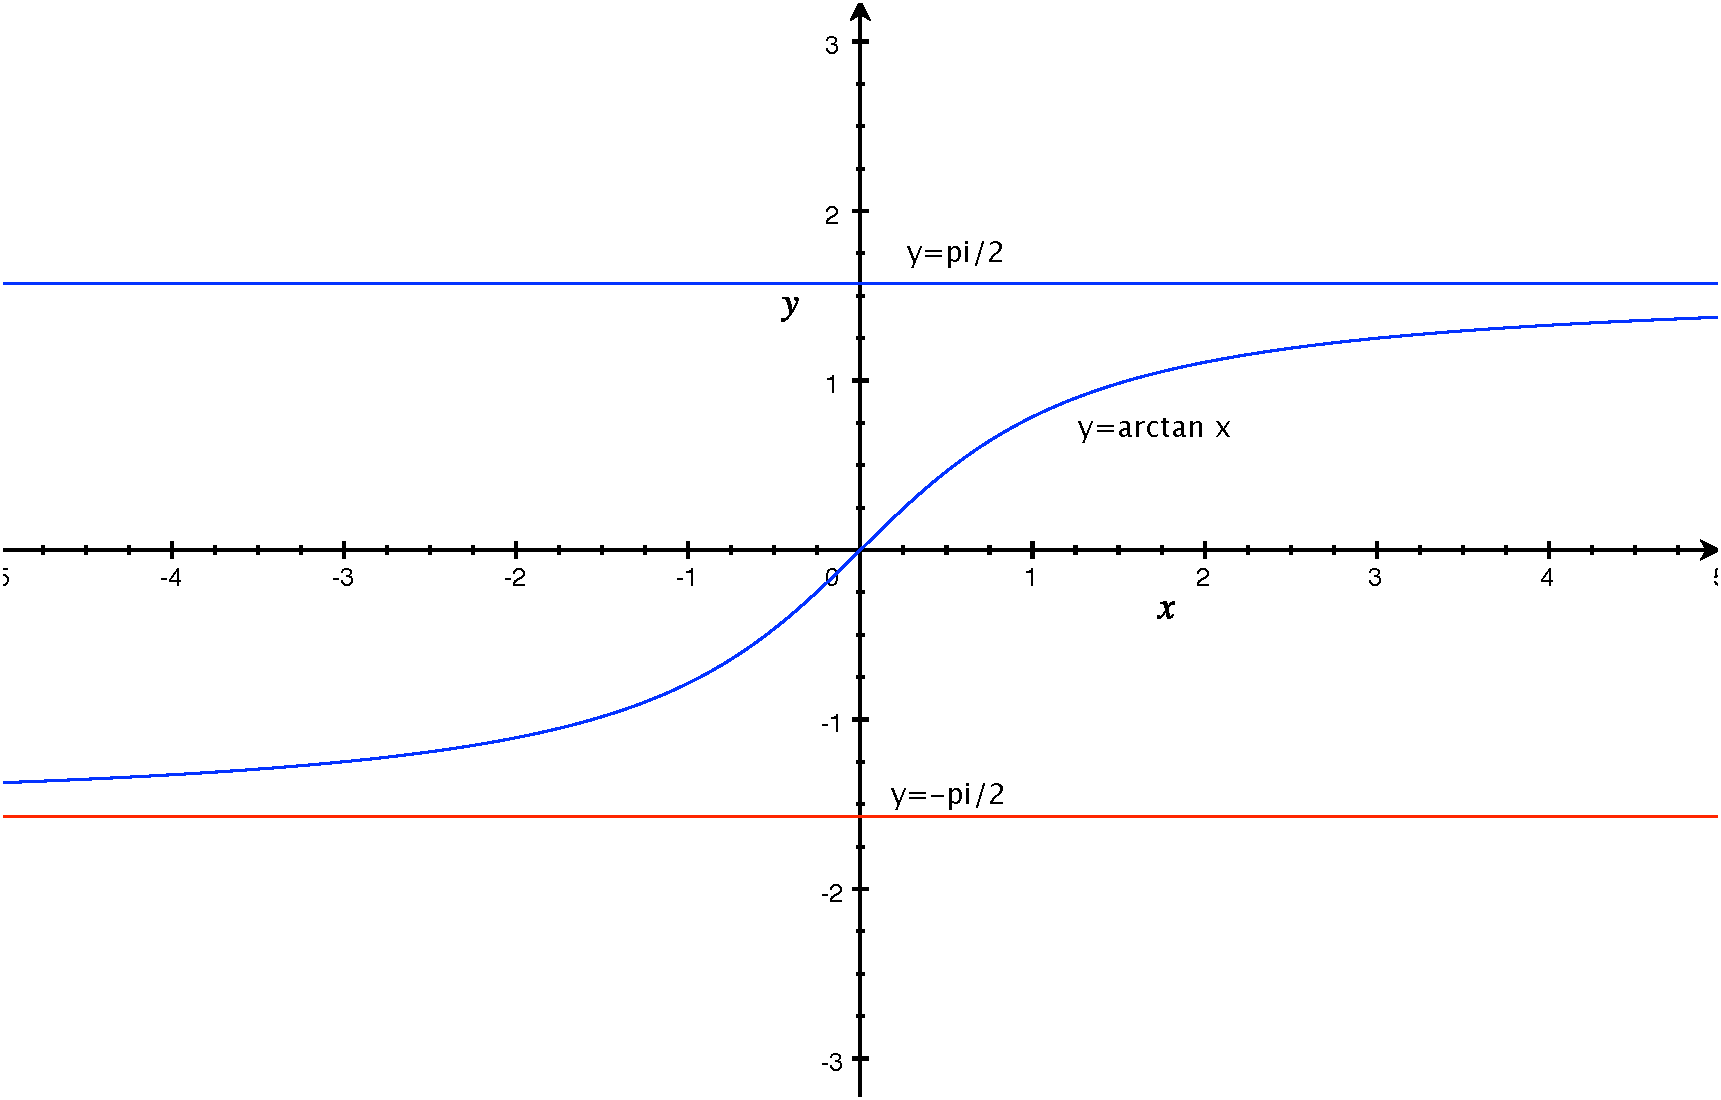
\includegraphics{./images/ch3/arctan.pdf}}
% \end{center}

\begin{center}
	\begin{overpic}[scale=0.3]{./images/ch3/arctan.pdf}
		\put(0,10){\b $\limx{-\infty}\arctan x=-\df{\pi}2$}
		\put(65,53){\b $\limx{+\infty}\arctan x=\df{\pi}2$}
	\end{overpic}
	
	$y=\arctan x$的图像与两条水平渐近线
\end{center}

\begin{thx}
	{\bf $x$趋于有限值时的函数极限}
	\begin{enumerate}%[(1)]
	  \item $\limx{x_0}f(x)=A\quad\Leftrightarrow\quad
	  \forall \e>0,\exists\delta>0,\forall
	  x\in {\b U_0(x_0,\delta)},|f(x)-A|<\e$
	  \item $\limx{x_0^+}f(x)=A\quad\Leftrightarrow\quad
	  \forall \e>0,\exists\delta>0,\forall x\in
	  {\b (x_0,x_0+\delta)},|f(x)-A|<\e$
	  \item $\limx{x_0^-}f(x)=A\quad\Leftrightarrow\quad
	  \forall \e>0,\exists\delta>0,\forall
	  x\in{\b (x_0-\delta,x_0)},|f(x)-A|<\e$
	\end{enumerate}
\end{thx}

无论是$x$趋于无穷时的极限还是$x$趋于有限值时的极限,定义的逻辑结构都是
一致的,唯一的不同就在于对$x$的范围的表述方式(有限领域和无穷领域的差别)。
抽象地说,以上的六个极限定义都是陈述了如下一个事实:$\limx{\Delta}f(x)=A$,
也即:随着$x$越来越靠近$\Delta$($\Delta$可以是以上六种趋势最终目标中
的任何一个),$f(x)$的值越来越靠近$A$;或者说,{\it\b 要使$f(x)$充分
靠近$A$,只需$x$充分靠近$\Delta$}。这与我们对数列极限的定义是完全一致的。

{\bf 例:}\ps{KD教材习题3.1-1}
根据图形判断极限的存在性
\begin{center}
	\resizebox{!}{4cm}{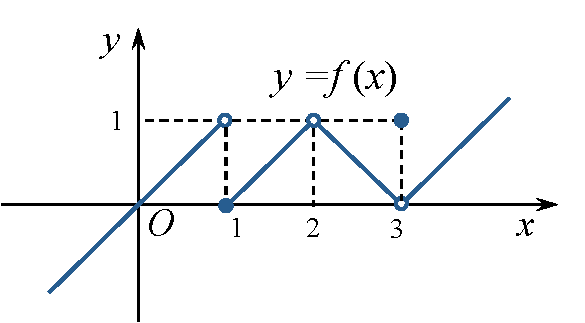
\includegraphics{./images/ch3/limxf.pdf}}
	
	$\limx{1}f(x)$\underline{不存在}
	\quad $\limx{2}f(x)$\underline{$=1$}
	\quad $\limx{1}f(x)$\underline{$=0$}
\end{center}

{\bf 思考:}{\b
	\begin{itemize}
	  \setlength{\itemindent}{1cm}
	  \item 为什么在定义中要求$0<|x-x_0|<\delta$,而不是$|x-x_0|<\delta$?
	  
	   \quad ({\it 因为极限表示的自变量趋于改点的过程中(而不是在该电上)函数值的变化趋势,
	   与函数在该点处的取值无关})
	  \item 符号$f(x_0+0),f(x_0-0)$与$f(x_0)$是何关系?
	  
	  \quad ({\it前两者分别表示左、右极限,最后一个是函数值,三者相互无关})
	\end{itemize}
}

{\bf 例:}证明:$\limx{x_0}\sin x=\sin x_0$。

[证]:对任意$\e>0$,令{\b$\delta=\e$},则当$0<|x-x_0|<\delta$时,有
$$|\sin x-\sin x_0|=2\left|\cos\df{x+x_0}2\right|
\left|\sin\df{x-x_0}2\right|\leq|x-x_0|<\delta=\e,$$
由函数极限定义,即证。\hfill $\Box$

{\bf 例:}证明:$\limx{1}x^2=1$。

[证]:对任意$\e>0$,令{\b$\delta=\min\left\{\df12,\e\right\}$},
\ps{令$\delta\leq\df12$,作用在于使得$|x+1|$有界}
则当$0<|x-1|<\delta$时,有
$$|x^2-1|=|(x+1)(x-1)|<\df32\cdot\delta<\df32\e,$$
由函数极限定义,即证。\hfill $\Box$

{\bf 例:}设$\limx{x_0}f(x)=A$,用定义证明:$\limx{x_0}[f(x)]^3=A^3$

[证]:对任意$\e>0$,由$\limx{x_0}f(x)=A$,存在$\delta>0$,对任意
$0<|x-x_0|<\delta$,有
$$|f(x)-A|<\e.$$
不妨设$\e<1$,由上式可知$0<|x-x_0|<\delta$时,有$|f(x)|<|A|+1$。

综上,记$C=(|A|+1)^2+(|A|+1)|A|+A^2$,则当$0<|x-x_0|<\delta$时,总有
\begin{align}
	|f^3(x)-A^3|&=|f(x)-A||f^2(x)+f(x)A+A^2|\notag\\
	&\leq |f(x)-A|[|f^2(x)|+|f(x)||A|+A^2]\notag\\
	&<\e[(|A|+1)^2+(|A|+1)|A|+A^2]=C\e\notag,
\end{align}
有极限的定义,即证。\hfill $\Box$

\begin{shaded}
	\begin{tcolorbox}
		{\bf 函数极限的反面说法}
		\begin{itemize}
		  \item {\it 当$x\to x_0$时$f(x)$不以$A$为极限:} 
		    $\exists\e_0>0,\forall\delta>0, \exists x^*\in
		    U_0(x_0,\delta),|f(x^*)-A|\geq\e_0$ 
		  \item {\it 当$x\to x_0$时$f(x)$无极限:}
			$\forall A\in\mathbb{R},\exists\e_0>0,\forall\delta>0, \exists x^*\in
		    U_0(x_0,\delta),|f(x^*)-A|\geq\e_0$ 
		\end{itemize}
	\end{tcolorbox}

	{\bf 例:}证明:Dirichlet函数在任意点处无极限。
	
	[证]:任取$x_0,A\in\mathbb{R}$,不妨设$A\ne 0$($A\ne 1$的情况同理可证)。
	
	令$\e_0=\df{|A|}2$,对任意$\delta>0$,由有理数的稠密性,总可以在
	$U_0(x_0,\delta)$内取得某个有理数$x^*$,从而$D(x^*)=0$,于是
	$$|D(x^*)-A|=|A|>\e_0,$$
	由上述的定义,可知当$x\to x_0$时$D(x)$无极限,又由$x_0$的任意性,可知
	$D(x)$处处无极限。\hfill $\Box$
	
	{\bf 思考题:}证明:函数$f(x)=xD(x)$只在$x=0$处收敛。

	注意,证明应该包括两个部分,一是证明$xD(x)$在$x=0$处收敛,二是证明
	$xD(x)$在任意$x\ne 0$处发散。
\end{shaded}

\subsection{函数极限的基本性质}

参考数列极限的性质,可以类似地证明函数极限的下列性质。

\begin{thx}
	{\bf 唯一性:}函数极限若存在,必唯一。
	
	{\bf 有界性:}
	\begin{enumerate}[(1)]
	  \item 若$\limx{+\infty}f(x)=A$,则$f(x)$当$x$充分大时有界
% 	  \ps{当$x$充分大时,等价于,存在$X$,当$x>X$时}
	  \item 若$\limx{x_0}f(x)=A$,则$f(x)$当$x$充分靠近$x_0$时有界
% 	  \ps{当$x$充分靠近$x_0$时,等价于,存在$\delta>0$,
% 	  当$x\in U_0(x_0,\delta)$时}
	\end{enumerate}
	{\bf 保号性:}
	\begin{enumerate}[(1)]
% 	  \setlength{\itemindent}{1cm}
	  \item 若$\limx{+\infty}f(x)=A>0$,则当$x$充分大时,$f(x)>0$
	  \item 若$\limx{x_0}f(x)=A>0$,则当$x$充分靠近时$x_0$时,$f(x)>0$
	\end{enumerate}
\end{thx}

{\bf 注意:}函数极限有界性和数列极限有界性的叙述存在的差异:
数列收敛则数列整体有界(数列极限中的数列整体都有界,
是由数列自身的“稀疏”特性所决定的),
函数收敛只能说明在趋近的过程中(或者充分靠近目标时)有界!

例如:极限$\limx{+\infty}\df1x=0$,但$\df1x$在定义域上无界;
类似地,$\limx{1}x=1$,但$x$显然也是无界的。

\begin{thx}
	{\bf 函数极限与数列极限的关系}({\kaishu Henie定理}):
	已知$\limx{x_0}f(x)=A$,若若数列$\{x_n\}$取值在$f(x)$的定义域内,
	且满足:$x_n\to x_0(n\to$ $\infty)$,$x_n\ne 0\;(n\in\mathbb{Z}_+)$,
	则必有$\limn f(x_n)=A$。
\end{thx}

[证]\ps{Henie(1821-1881),德国数学大师Weierstrass的学生。
1872年证明:有界闭区间上的连续函数必是一致连续的。也即,如果把函数的定义限定在闭区间上,
连续和一致连续的差别将随之消失。} 
:已知$\limx{x_0}f(x)=A$,故对任意$\e>0$,存在$\delta>0$,
使对任意$x\in U_0(x_0,\delta)$,都有$|f(x)-A|<\e$。

设$\limn x_n=x_0$,则以上的$\delta>0$,存在$N\in\mathbb{Z}_+$,
使对任意$n>N$,都有$|x_n-x_0|<\delta$。从而,当$n>N$时,必有
$$|f(x_n)-A|<\e.$$
即证。\hfill $\Box$

对于$x\to x_0^+$和$x\to x_0^-$的情形,该定理显然也成立。

与上一节子数列有关收敛性质的用途一样,Henie定理的用途更多地是证明函数极限不存在。
当然,有时遇到一些不方便计算的数列极限,也可能将其转化为对应的函数极限来计算
\ps{由于计算函数极限有类似L'Hospital法则和Taylor公式这样的工具,相对来说
比计算数列极限方法更多样}。

{\bf 例:}{\b 证明:$f(x)=\sin\df 1x$当$x\to 0$时无极限。}\ps{KD教材3.2.2节-例8}

[证]:令
$$x^{(1)}_n=\df1{n\pi},\quad
x^{(2)}_n=\df1{2n\pi+\df{\pi}2},\quad n\in\mathbb{Z}_+$$ 
显然,$\limn x^{(1)}_n=\limn x^{(2)}_n=0$,且
$$f(x^{(1)}_n)\equiv0,\quad f(x^{(2)}_n)\equiv1,$$
进而
$$\limn f(x^{(1)}_n)=0\ne1=\limn f(x^{(2)}_n),$$
由Henie定理,即知极限不存在。\hfill $\Box$

\begin{center}
	\resizebox{!}{5cm}{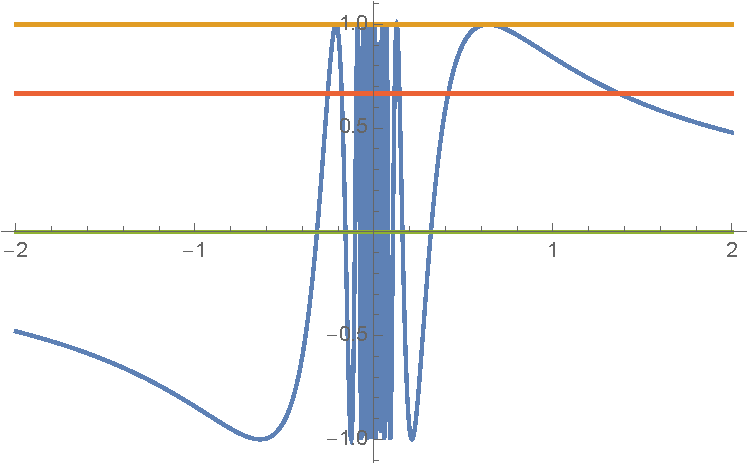
\includegraphics{./images/ch3/sin1x.pdf}}
	
	{\it 以上所取的$x^{(1)}_n$和$x^{(2)}_n$分别取自图上绿色和黄色水平线与
	函数$\sin\df1x$的交点,事实上,对于任意的$a\in[-1,1]$(红色水平线),
	都可以取得类似的点列,用于构造证明所需的收敛到不同值得函数值数列,请思考以下如何写
	出其表达式?
	$$x^{(a)}_n=\df1{2n\pi+\arcsin a},\quad n\in\mathbb{Z}_+$$}
\end{center}

% \begin{shaded}
	{\bf 例:}用Henie定理证明Dirichlet函数在任意点处无极限。
	
% 	{\bf 命题:}对任意$x_0\in\mathbb{R}$,都存在这样的两个数列
% 	$\{x_n^{(1)}\}$和$\{x_n^{(2)}\}$,满足
% 	$$x_n^{(1)}\in\mathbb{Q},\;x_n^{(2)}\notin\mathbb{Q}\;(n\in\mathbb{Z}_+),$$
% 	且
% 	$$\limn x_n^{(1)}=\limn x_n^{(2)}=x_0.$$
% 	
% 	{\bf 思考:}试给出$\{x_n^{(1)}\}$和$\{x_n^{(2)}\}$的通项表达式。
	
	[证]:
% 	1)若$x_0\in\mathbb{Q}$,可令
% 	$$x_n^{(1)}=x_0+\df1n,\quad
% 	x_n^{(2)}=x_0+\df{\sqrt2}n,\;(n\in\mathbb{Z}_+)$$
% 	2)若$x_0\notin\mathbb{Q}$,可令
% 	$$x_n^{(1)}=[x_0]+x_0\mbox{\it 小数部分的前}n\mbox{\it 位},
% 	\;(n\in\mathbb{Z}_+)$$
% 	例如$x_0=\pi=3.1415926\ldots$,则
% 	$$x_1^{(1)}=3.1,\;x_2^{(1)}=3.14,\;x_3^{(1)}=3.141,\;
% 	x_4^{(1)}=3.1415,\;\ldots$$
% 	另,
% 	$$x_n^{(2)}=x_0+\df1n,\;(n\in\mathbb{Z}_+)$$
% 	
% 	{\bf 又解:}
	对任意$x_0$,定义
	$$x_n=[x_0]+x_0\mbox{\it 小数部分的前}n\mbox{\it 位},$$
	$$x_n^{(1)}=x_n+\df1n,$$
	$$x_n^{(2)}=x_n+\df{\sqrt2}n,$$
	显然$\{x_n^{(1)}\}$和$\{x_n^{(2)}\}$分别为趋于$x_0$的有理和无理数列,而
	$$\limn D(x_n^{(1)})=1\ne0=\limn D(x_n^{(2)}),$$
	从而由Hiene定理,即证。\hfill $\Box$
% \end{shaded}

{\bf 例:}设在$(0,+\infty)$上,恒有$f(x^2)=f(x)$,且
$$\limx{0^+}f(x)=\limx{+\infty}f(x)=f(1)$$
证明:$f(x)=f(1)\,(x\in(0,+\infty))$

[提示]:对任意$x_0>1$,都有
$$f(x_0)=f(x_0^2)=f(x_0^4)=\ldots=\limn f(x_0^{2^n})=\limx{+\infty}f(x)=f(1).$$
对任意$x_0<1$,都有
$$f(x_0)=f(x_0^2)=f(x_0^4)=\ldots=\limn f(x_0^{2^n})=\limx{0^+}f(x)=f(1).$$

\begin{ext}
	{\centering\bf 课后作业}
	
	\begin{enumerate}  
	  \item 用定义证明如下极限:
	  \begin{enumerate}[(1)]
	    \item $\limx{-2}{x^2}=4$;
	    \item $\limx{\infty}\df{\sin x}{\sqrt x}=0$;
	    \item $\limx{\infty}\df{x+\sin x}{x+\cos x}=1$.
	  \end{enumerate}
	  \item 证明:$f(x)=xD(x)$仅当$x=0$时极限存在。($D(x)$表示Dirichlet函数)
	\end{enumerate}
\end{ext}

\section{无穷小与无穷大}

\subsection{无穷小}

以下$\Delta$表示$x_0,x_0^+,x_0^-,\infty,+\infty,-\infty$中的任意一个。

\begin{thx}
	若$\limx{\Delta}f(x)=0$,则称{\bf $f(x)$为$x\to\Delta$时的无穷小},记为
	$${\b f(x)=\circ(1),\;(x\to\Delta).}$$
\end{thx}

注意,{\b 谈到无穷小,一定是和某个变化过程相对应的}。例如:$f(x)=x-1$是$x\to 1$时的
无穷小,但不是$x\to 2$时的无穷小。

显然,常值函数$f(x)\equiv 0$是任何过程中的无穷小。

利用函数极限和无穷小的定义,容易证明:
\begin{thx}
	{\bf 定理:}$\limx{\Delta}f(x)=A\Leftrightarrow f(x)=A+\alpha$,
	其中$\alpha$是$x\to\Delta$时的无穷小。
\end{thx}
该结论也可以简写为:
$$\limx{\Delta}f(x)=A\quad\Leftrightarrow\quad f(x)=A+\circ(1)$$
% \begin{enumerate}[(1)]
%   \setlength{\itemindent}{1cm}
%   \item 
%   \item $\limx{\Delta}f(x)=A$,$\alpha$是$x\to\Delta$时的无穷小,则$\alpha f(x)$
%   也是$x\to\Delta$时的无穷小,也即:{\it 在同一过程中,无穷小和有界函数的乘积仍为无穷小}。
% \end{enumerate}

进一步地,有无穷小的定义,不难证明:

\begin{thx}
	{\bf 无穷小的性质}
	\begin{enumerate}%[(1)]
	%   \setlength{\itemindent}{1cm}
	  \item 有限多个无穷小的和也是无穷小;
	  \item 有界函数与无穷小的乘积是无穷小;
	  \item 任意多个无穷小的乘积是无穷小。
	\end{enumerate}
\end{thx}

{\bf 注:}无穷多个无穷小相加未必还是无穷小,而可能是任意的结果,例如:当$n\to\infty$时
$$\underbrace{\df1n+\df1n+\ldots+\df1n}_{n\mbox{\footnotesize 个}}=1\to1,$$
$$\underbrace{\df1{n^2}+\df1{n^2}+\ldots+\df1{n^2}}
_{n\mbox{\footnotesize 个}}=\df1n\to0,$$
$$\underbrace{\df1n+\df1n+\ldots+\df1n}
_{n^2\mbox{\footnotesize 个}}=n\to+\infty.$$

\subsection{无穷大}

无穷大意味着在某个过程中,函数的绝对值会无限增大,这同时也就意味着其倒数会趋于零。

\begin{thx}
	若$\limx{\Delta}\df1{f(x)}=0$,则称{\bf $f(x)$为$x\to\Delta$时的无穷大}。
\end{thx}

这里我们的定义和同济的教材上略有区别,但是完全等价。

需要注意的是,{\b 无穷大和无界是不同的}。例如:$f(x)=x$和$g(x)=x\sin x$都是$x\to\infty$时
的无界量(即:只要$x$充分远离原点,则函数值可以超过任何事先给定的值),但前者是该过程中的
无穷大,后者不是。

此外,{\b 要注意无穷大有正负之分,而无穷小没有。}

无穷大的等价定义:$f(x)$为$x\to\Delta$时的无穷大,也即:
对于任意$M>0$,当$x$充分靠近$\Delta$时,总有$|f(x)|>M$。
下面就$x\to x_0$的情况给出证明。

\begin{thx}
	{\bf 定理:}$f(x)$为$x\to x_0$时的无穷大,当且仅当:
	对于任意$M>0$,存在$\delta>0$,使对任意$x\in U_0(x_0,\delta)$,
	总有$|f(x)|>M$。
\end{thx}

[证]:任取$M>0$,令$\e=\df1M$。由无穷大的定义,$\limx{\Delta}\df1{f(x)}=0$,故对
此$\e$,存在$\delta>0$,使对任意$x\in U_0(x_0,\delta)$,总有
$$\left|\df1{f(x)}\right|<\e\quad\Rightarrow |f(x)|>\df1{\e}=M.$$
即证。\hfill $\Box$

{\b$x\to x_0$或$x_0^+,x_0^-$时的无穷大对应的是函数曲线的{\bf 铅直渐近线}}。例如:
$\limx{0}\df1x=0$,故$x=0$是$f(x)=\df1x$的铅直渐近线;
$\limx{\pi/2^+}\tan x=-\infty$,故$x=\pi/2$是$f(x)=\tan x$的铅直渐近线。

{\bf 例:}设当$x\to x_0$时,$f(x)$不是无穷大,则下列命题中正确的是(D)
\begin{enumerate}[(A)]
  \setlength{\itemindent}{1cm}
  \item 若$g(x)$是$x\to x_0$时的无穷小,则$f(x)g(x)$必为$x\to x_0$时的无穷小
  \item 若$g(x)$不是$x\to x_0$时的无穷小,则$f(x)g(x)$必不是$x\to x_0$时的无穷小
  \item 若$g(x)$在$x_0$的某邻域内无界,则$f(x)g(x)$必为$x\to x_0$时的无穷大
  \item 若$g(x)$在$x_0$的某邻域内有界,则$f(x)g(x)$必不是$x\to x_0$时的无穷大
\end{enumerate}

[提示]:不妨以$x\to0$为例,

(A)反例:$f(x)=\df1x\sin\df1x$,$g(x)=x$;

(B)反例:$f(x)=0$,$g(x)=1$;

(C)反例:$f(x)=g(x)=\df1x\sin\df1x$;

(D)反证法:若$f(x)g(x)$是无穷大,则$\limx0\df1{f(x)g(x)}=0$,$g(x)$是有界量,
有界量与无穷小的乘积仍为无穷小,故$f(x)=\df1{f(x)g(x)}\cdot g(x)$为无穷小,
从而$f(x)$是无穷大,与已知矛盾!

\begin{ext}
	{\centering\bf 课后作业}
	
	\begin{enumerate}  
	  \item 证明:函数$y=\df1x\sin\df1x$在区间$[0,1]$内无界,但它不是$x\to 0+$
	  时的无穷大。
	  \item 求函数$y=\df1{1-x^2}$的水平渐近线和铅直渐进线。
	  \item 判断:无穷小除以无界量一定是无穷小吗?如果正确,请给出证明;如果错误,请举反例。
% 	  \begin{enumerate}[(1)]
% 	    \item $\limx{-2}{x^2}=4$;
% 	  \end{enumerate}
	\end{enumerate}
\end{ext}

\section{极限运算法则}

以下讨论的所有性质都是指在同一个$x\to\Delta$的极限过程中。

\subsection{极限的四则运算}

利用无穷小的基本的性质,我们可以很方便地证明:

\begin{thx}
	{\bf 极限的四则运算性质:}
	若相关极限都有意义,且符合代数运算的基本条件,则极限运算总可以
	和有限多次的四则运算交换次序。
\end{thx}

显然,以上的结论同时适用于各种函数极限和数列极限。

如果不是有限次数的四则运算,若随意交换极限运算和四则运算的次序,
则可能出现如下的错误:
{\b
\begin{align*}
	1&=\limn1=\limn\left(\underbrace{\df1n+\df1n+\ldots+\df1n}
	_{n\mbox{\footnotesize 个}}\right)\\
	&=\underbrace{\limn\df1n+\limn\df1n+\ldots+\limn\df1n}
	_{n\mbox{\footnotesize 个}}\\
	&=\underbrace{0+0+\ldots+0}_{n\mbox{\footnotesize 个}}=0
\end{align*}
}

相当于$n$落在了极限符号之外,显然错误!!


{\bf 例:}计算极限
$$\limx{\infty}\df{3x^3+2x-1}{4x^3+6x^2+9}$$

[解]:
\begin{align}
	\limx{\infty}&\df{3x^3+2x-1}{4x^3+6x^2+9}
	=\limx{\infty}\df{3+2\frac1{x^2}-\frac1{x^3}}
	{4+6\frac1x+9\frac1{x^3}}
	=\df{\limx{\infty}\left(3+2\frac1{x^2}-\frac1{x^3}\right)}
	{\limx{\infty}\left(4+6\frac1x+9\frac1{x^3}\right)}\notag\\
	&=\df{\limx{\infty}3+\limx{\infty}2\frac1{x^2}-\limx{\infty}\frac1{x^3}}
	{\limx{\infty}4+\limx{\infty}6\frac1x+\limx{\infty}9\frac1{x^3}}
	=\df{\limx{\infty}3+\limx{\infty}2\limx{\infty}\frac1{x^2}
	-\limx{\infty}\frac1{x^3}}
	{\limx{\infty}4+\limx{\infty}6\limx{\infty}\frac1x
	+\limx{\infty}9\limx{\infty}\frac1{x^3}}\notag\\
	&=\df{3+2\cdot 0-0}{4+6\cdot 0+9\cdot 0}=\df34\notag
\end{align}
\hfill $\Box$

在日常的解题中,计算过程显然不必都如此详细。

对于与该例类似的极限问题,我们有如下的结论,在今后的极限计算中可以直接应用:

\begin{thx}
	{\bf 有理函数当$x\to+\infty$时的极限:}
	设$P(x)$和$Q(x)$分别为$m$和$n$次多项式函数,且其最高次项系数分别为
	$a,b$,$ab\ne 0$,则
	$$
		\limx{+\infty}\df{P(x)}{Q(x)}=
		\left\{\begin{array}{ll}
			a/b, & m=n;\\
			0, & m<n;\\
			\mbox{不存在}, & m>n.
		\end{array}\right.
	$$
\end{thx}

{\bf 思考:}有理函数当$x\to 0$时的极限如何计算?有什么规律?

{\bf 定理:}{\b 初等函数运算可以和极限运算交换次序}
\ps{后续章节中,我们将学习到因为初等函数在其定义区间内均连续,故初等函数运算可以和
极限运算交换次序}

{\bf 例:}计算极限
$$\limn\df{\cos^n\theta-\sin^n\theta}{\cos^n\theta+\sin^n\theta}\quad
(0\leq\theta\leq\df{\pi}{2})$$

[提示]:根据$\theta$的取值范围,决定是分子分母同时除以$\sin^nx$还是$\cos^nx$,结果
$$\mbox{原式}=\left\{\begin{array}{ll}
-1,& 0<\theta<\df{\pi}4\\
0,& \theta=\df{\pi}4\\
1,& \df{\pi}4<\theta<\df{\pi}2
\end{array}\right.$$

{\bf 例:}$|x|<1$,计算
$$\limn(1+x)(1+x^2)\ldots(1+x^{2^n})$$

[提示]:
$$(1+x)(1+x^2)\ldots(1+x^{2^n})=\df{(1-x)(1+x)(1+x^2)\ldots(1+x^{2^n})}{1-x}
=\df{1-x^{2^{n+1}}}{1-x}$$

{\bf 例:} $\limn\left(\sqrt{n+3\sqrt n}-\sqrt{n-\sqrt{n}}\right)=2$
\hfill({\it 分子有理化})

{\bf 例:} $\limn\left(\sqrt[3]{n^3+2n^2+1}-n\right)=\df23$
% \ps{$a^n-b^n=(a-b)(a^{n-1}+a^{n-2}b+\ldots+b^{n-1})$}
\hfill({\it 分子有理化})

[提示]:利用公式$a^n-b^n=(a-b)(a^{n-1}+a^{n-2}b+\ldots+b^{n-1})$
进行分子有理化:
$$\mbox{原式}=\limn\df{2n^2+1}{(n^3+2n^2+1)^{\frac23}
+(n^3+2n^2+1)^{\frac13}n+n^2}$$

{\bf 例:} $\limn\left(1-\df1{2^2}\right)\left(1-\df1{3^2}\right)\ldots
\left(1-\df1{n^2}\right)=\df12$\hfill({\it 因式分解,消去公共部分})

{\bf 例:} $\limn\sin^2\left(\pi\sqrt{n^2+n}\right)$\hfill({\it 周期性结合分子有理化})

{\bf 例:} $\limn\df32\cdot\df54\cdots\df{2^n+1}{2^n}
=\limn2\left(1-\df12\right)\left(1+\df12\right)\left(1+\df1{2^2}\right)
\ldots\left(1+\df1{2^n}\right)=2$

{\bf 例:} $\sqrt{n+\sqrt{n+\sqrt n}}-\sqrt n\to\df12,\;(n\to\infty)$
\hfill({\it 分子有理化})

{\bf 例:}确定常数$a,b$的值,使得$\limx1\df{x^2+ax+b}{x-1}=3$。

[解]:
% 由极限的四则运算法则,
$$1+a+b=\limx1{x^2+ax+b}=\limx1\df{x^2+ax+b}{x-1}\limx1{x-1}=3\cdot0=0.$$
原式可化为
$$\limx1\df{(x-1)^2+(a+2)(x-1)+(a+b+1)}{x-1}=3,$$
也即
$$\limx1(x-1)+(a+2)+\limx1\df{(a+b+1)}{x-1}=3,$$
该式成立,当且仅当
$$
	\left\{\begin{array}{l}
		a+2=3,\\
		a+b+1=0.
	\end{array}\right.
$$
从而可以解得$a=1,b=-2$,即为所求。\hfill$\Box$

\subsection{复合函数的极限}

\begin{thx}
	{\bf 复合函数的极限(情形I):}设
	$$\limx{x_0}g(x)=u_0,\quad\lim\limits_{u\to u_0}f(u)=A,$$
	且在$x_0$附近$g(x)\ne u_0$,则
	$$\limx{x_0}f[g(x)]=A.$$
\end{thx}

[证]:对任意$\e>0$,由$\lim\limits_{u\to u_0}f(u)=A$可知,存在
$\delta_1>0$,对任意$u\in U_0(u_0,\delta_1)$,均有
$$|f(u)-A|<\e.$$
对以上的$\delta_1>0$,由$\limx{x_0}g(x)=u_0$,存在$\delta>0$,
使对任意$x\in U_0(x_0,\delta)$,均有
$$|g(x)-u_0|<\delta_1,$$
又由已知,在$x_0$附近$g(x)\ne u_0$,不妨设当$x\in U_0(x_0,\delta)$
时$g(x)\ne u_0$,从而可知此时$g(x)\in U_0(u_0,\delta_1)$,进而可得
$$|f(g(x))-A|<\e.$$
即证。\hfill$\Box$

{\bf 思考:}为什么定理条件中要求“在$x_0$附近$g(x)\ne u_0$”?
  
  答:因为$f(x)$可能在$x_0$处的定义与极限值无关,例如:
  $$f(x)=\left\{\begin{array}{ll}
  1,&x\ne0\\0,&x=0
  \end{array}\right.$$
  $g(x)\equiv 0$,则$f(g(x))\equiv0$,从而$\limx{0}f(g(x))=0$,
  而不是如定理所述$\limx{0}f(g(x))=1$

直观的理解,以上的结论告诉我们:若相关极限都存在,且满足一定的条件,
则极限运算可以和函数运算交换次序。

显然,这个结论可以类似地推广到$x\to\infty$的情形,例如:

\begin{thx}
	{\bf 复合函数的极限(情形II):}设
	$$\limx{+\infty}g(x)=u_0,\quad\lim\limits_{u\to u_0}f(u)=A,$$
	且当$x$充分大时$g(x)\ne u_0$,则
	$$\limx{+\infty}f[g(x)]=A.$$
\end{thx}
又比如
\begin{thx}
	{\bf 复合函数的极限(情形III):}设
	$$\limx{x_0}g(x)=+\infty,\quad\lim\limits_{u\to+\infty}f(u)=A,$$
	则
	$$\limx{x_0}f[g(x)]=A.$$
\end{thx}
想一想为什么最后这个命题似乎比前面的两个都少了一个条件?

{\bf 例:}判断与分析
\begin{enumerate}[(1)]
  \setlength{\itemindent}{1cm}
  \item 若$x\to x_0$时,$f(x)$有极限,$g(x)$无极限,则当$x\to x_0$时,以下哪些函数必无极限:
  $$f(x)g(x),\quad [g(x)]^2,\df{g(x)}{f(x)}, f(x)+g(x)$$ 
  \item 若$\limx{x_0}g(x)=A,\lim\limits_{u\to A}f(u)=B$,是否必有
  $\limx{x_0}f[g(x)]=B$?
  \item 若$\limx{x_0}f(x)g(x)=0$,则当$x\to
  x_0$时, $f(x),$ $g(x)$之一必趋于$0$.
\end{enumerate}

[提示]:(1)不妨以$x\to0$时的极限为例:

$f(x)g(x)$可能收敛,例如:$f(x)=x,g(x)=D(x)$;

$[g(x)]^2$可能收敛,例如:$g(x)=\mathrm{sgn}(x)$;

$\df{g(x)}{f(x)}$必无极限。反证法:若该极限存在,则由极限的乘法规则
$$\limx0g(x)=\limx0{g(x)}{f(x)}\limx0f(x)$$
也存在,与已知矛盾;

$f(x)+g(x)$比无极限。证法与前一种情况类似。

(2)错!反例:
$$f(x)=\left\{\begin{array}{ll}
  1,&x\ne0\\0,&x=0
\end{array}\right.$$
$g(x)\equiv 0$,则$f(g(x))\equiv0$,从而$\limx{0}f(g(x))=0\ne 1$

(3)错!反例:$f(x)=D(x)$,$g(x)=1-D(x)$,则$f(x)g(x)\equiv 0$。

\begin{ext}
	{\centering\bf 课后作业}
	
	\begin{enumerate}  
	  \item 设$\{a_n\},\{b_n\},\{c_n\}$均为非负数列,且
	  $$\limn a_n=0,\quad \limn b_n=1,\quad \limn c_n=\infty.$$
	  判断以下说法的正误。正确的,给出证明;错误的,举一个反例。
	  \begin{enumerate}[(1)]
	    \item $n$充分大时,$a_n<b_n<c_n$;
	    \item $\limn a_nc_n$必存在;
	    \item $\limn b_nc_n$必不存在(极限为$\infty$属于极限不存在)。
	  \end{enumerate}
	  \item 计算如下极限
	  \begin{enumerate}[(1)]
	    \item $\limx{1}\left(\df1{1-x}-\df3{1-x^3}\right)$;
	    \item $\limx0\df{(h+x)^3-h^3}x$;
	    \item $\limx{\infty}\df{\arctan x}{x^2}$;
	    \item $\limx{+\infty}\df{\sqrt[3]{x+\sqrt{x+x^3}}}{\sqrt{x+1}}$;
	    \item $\limx4\df{\sqrt{2x+1}-3}{\sqrt{x-2}-\sqrt2}$;
	    \item $\limx0\df{\sqrt[3]{x+1}-1}x$;
	    \item $\limx0\df{\sqrt{1+x}+\sqrt{1-x}-2}{x^2}$;
	    \item $\limx{+\infty}\df{\ln(2+e^{3x})}{\ln(3+e^{2x})}$;
	    \item $\limx{+\infty}x(\sqrt{x^2+1}-x)$;
	    \item $\limx{-\infty}x(\sqrt{x^2+1}-x)$.
	  \end{enumerate}
	  \item 确定常数$a,b$的值,使得
	  $\limx{\infty}\left(\df{x^2}{x+1}-ax-b\right)=0$。
	\end{enumerate}
\end{ext}

\section{极限存在准则与两个重要极限}

\subsection{夹逼准则}

有时也叫{\it 迫敛准则}或者{\it 三明治定理}。

\begin{thx}
	{\bf 准则I:}设对任意$n\in\mathbb{N}$,$x_n\le a_n\le y_n$,
	且$\{x_n\},\{y_n\}$收敛于相同的极限$a$,则$\limn a_n=a$。
\end{thx}

\begin{center}
	\resizebox{!}{4cm}{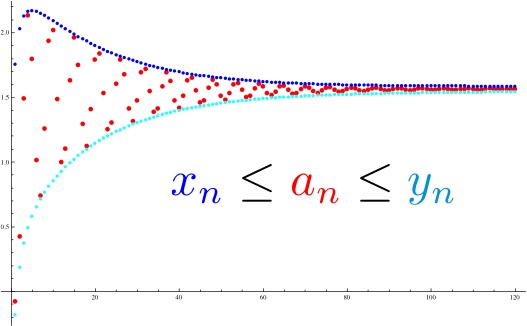
\includegraphics{./images/ch2/xay_n.jpg}}
\end{center}

{\bf 例:}证明:$\limn (\sqrt{n+1}-\sqrt{n})=0$。

[证](夹逼准则):注意到
$$0<\sqrt{n+1}-\sqrt{n}={\b\df1{\sqrt{n+1}+\sqrt{n}}
\leq\df 1{\sqrt{n}}},$$
又
$$\limn 0=\limn\df 1{\sqrt{n}}=0,$$
故由夹逼准则,可知$\limn (\sqrt{n+1}-\sqrt{n})=0$。\hfill $\Box$

对比一下用定义证明的过程:

[证](定义):对任意$\e>0$,令$N=[1/\e^2]+1$,则对任意$n>N$,总有
$$\left|\sqrt{n+1}-\sqrt{n}-0\right|
={\b\df1{\sqrt{n+1}+\sqrt{n}}\leq\df 1{\sqrt{n}}}
<\df 1{\sqrt{N}}<\df 1{\sqrt{1/\e^2}}=\e,$$
由此可知$\limn (\sqrt{n+1}-\sqrt{n})=0$。\hfill $\Box$

不难发现,两个证明中最关键的放缩步骤是完全一致的,而使用夹逼准则时,可以直接
使用一些已知的或“简单的”极限结论,避免了推导$N$的繁琐步骤,因此过程显得更加
简洁也更容易理解。

{\bf 思考:}证明:$\limn [(n+1)^k-{n}^k]=0$,其中$0<k<1$。

[提示]:$n^k\left[\left(1+\df1n\right)^k-1\right]
<n^k\left(1+\df1n-1\right)=n^{k-1}\to 0\;(n\to\infty)$

{\bf 例:}\ps{KD教材2.2.3节-例6,重点掌握结论!}
证明:
\begin{thx}
	{\bf 常用极限:}若$a>0$为常数,则$\limn \sqrt[n]{a}=1$。
\end{thx}
[证]:$a=1$时结论显然成立。

下面考虑$a>1$的情况。此时,显然有$h_n=\sqrt[n]a-1>0$,故
$$a=(1+h_n)^n=1+nh_n+\df{n(n-1)}2h_n^2+\ldots+h_n^n>1+nh_n,$$
进而
$$0<h_n<\df{a-1}n,$$
不等式左右两端当$n\to\infty$时极限均为$0$,故由夹逼准则,$\limn h_n=0$,也即
$$\limn\sqrt[n]a=1.$$

最后,对于$0<a<1$的情形,令$b=\df1a$,则
$$\limn\sqrt[n]a=\limn\sqrt[n]{\df1b}
=\df1{\limn\sqrt[n]b}=\df11=1.$$
至此,证毕。\hfill$\Box$

{\bf 思考:}利用本例类似的方法,证明:
\begin{thx}
	$$\limn\sqrt[n]n=1.$$
\end{thx}

{\bf 例:}计算极限
\begin{enumerate}[(1)]
  \setlength{\itemindent}{1cm}
  \item $\limn\sqrt[n]{n^5}=1$
  
  [提示]:$\mbox{原式}=\left(\limn\sqrt[n]{n}\right)^5$.
  \item $\limn\sqrt[n]{3^n+5^n}=1^5=1$.
  
  [提示]:$5=\sqrt[n]{5^n}<\sqrt[n]{3^n+5^n}
  <\sqrt[n]{2\cdot 5^n}=\sqrt[n]2\sqrt[n]{5^n}=\sqrt[n]2\cdot5$.
  
  \begin{thx}
	  {\bf 常用极限:}设$a_k\geq0,\;(k=1,2,\ldots)$,则$\limn\sqrt[n]
	  {\sum\limits_{k=1}^na_k^n}=\max\limits_{1\leq k\leq n}a_k.$
  \end{thx}
  
  \item $\limn\sqrt[n^2]{5^n+1}=1$
  \item 已知$a>b>0$,$\limn\sqrt[n]{\df1{a^n}+\df1{b^n}}=\df1b$
  \item $\limn\sqrt[n]{n^5+5^n}=5$
  \item $\limn\df{\sqrt{n+\sqrt n}-\sqrt n}{\sqrt[n]{3^n+5^n+7^n}}=\df1{14}$
  \item $\limn\left(\df1{n+1}+\df1{\sqrt{n^2+1}}+\ldots
	+\df1{\sqrt[n]{n^n+1}}\right)=1$
  \item $\limn n^2\left(\df kn-\df1{n+1}-\df1{n+2}
	-\ldots-\df1{n+k}\right),\;k\in\mathbb{Z}_+$
\end{enumerate}

\begin{thx}
	{\bf 准则I':}设在$x_0$的某邻域内,恒有
	$$\varphi(x)\leq f(x)\leq\psi(x), $$
	且$\limx{x_0}\varphi(x)=\limx{x_0}\psi(x)=A$,则
	$$\limx{x_0}f(x)=A.$$
\end{thx}

{\bf 注:}该准则显然可以推广到$x$趋于无穷的情形。

{\bf 例:}(重要极限)证明:({\color{red}以下$x$取弧度值!})
\begin{thx}
	$$\limx{0}\df {\sin x}x=1$$
\end{thx}

[证]:
\begin{center}
	\resizebox{!}{5cm}{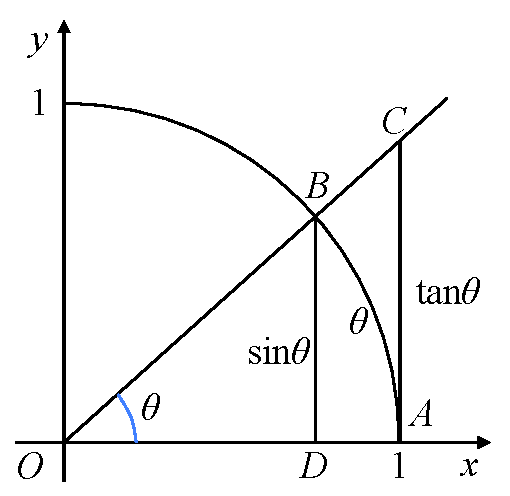
\includegraphics{./images/ch3/xsintan.pdf}}
\end{center}

如图,$\theta>0$时,显然弧$AB$的长度大于直线$BD$,即$\sin\theta<\theta$;
又扇形$ABO$的面积$\df12\theta$小于三角形$ACO$的面积$\df12\tan\theta$,
从而$\theta<\tan\theta$。由
$$\sin\theta<\theta<\tan\theta,$$
两边都除以$\sin\theta$,然后倒置,可得
$$1<\df{\sin\theta}{\theta}<\cos\theta,$$
注意到当$\theta\to 0^+$时,不等式左右极限都为$1$,故
$\lim\limits_{\theta\to0^+}\df{\sin\theta}{\theta}=1$。
又$\df{\sin x}x$为偶函数,故立即可得
$\lim\limits_{\theta\to0^-}\df{\sin\theta}{\theta}=1$。

综上即证。\hfill$\Box$

从这个极限出发可得到的一些常用的极限:
\begin{thx}
	\begin{enumerate}[(1)]
% 	  \setlength{\itemindent}{1cm}
	  \item $\limx{0}\df{\sin\sin x}{\sin x}=1$ 
	  \item $\limx 0\df{1-\cos x}{x^2}=\df12$ 
	  \item $\limx 0\df{\sin mx}{\sin nx}=\df mn$
	  \item $\limx 0\df{\tan x}{x}=1$
	  \item $\limx 0\df{\arcsin x}x=1$
	  \item $\limx 0\df{\arctan x}x=1$
	  \item $\limx a\df{\sin x-\sin a}{x-a}=\cos a$
	\end{enumerate}
\end{thx}

{\bf 例:}设$f(x)=\sum\limits_{i=1}^na_i\sin
ix$,其中$a_i(i=1,2,\ldots,n)$为常数,且对任意$x\in\mathbb{R}$, $|f(x)|\leq |\sin x|$,证明:
$$\left|a_1+2a_2+\ldots+na_n\right|\leq 1$$

[证]:由已知,$x\ne 0$时,总有
$$\left|\df{f(x)}{\sin x}\right|\leq 1,$$
也即
$$\left|a_1+a_2\df{\sin 2x}{\sin x}+\ldots
+a_n\df{\sin nx}{\sin x}\right|\leq 1.$$
注意到对任意$k=2,3,\ldots,n$,总有$\limx{0}\df{\sin kx}{\sin x}=k$,
且对任意函数$f(x)$,由$\limx{0}f(x)=a$总可推出$\limx{0}|f(x)|=|a|$,故
在前式两边同时令$x\to0$,由极限的保号性可得
\begin{align*}
	|a_1&+2a_2+\ldots+na_n|
	=\left|a_1+a_2\limx0\df{\sin 2x}{\sin x}+\ldots
	+a_n\limx0\df{\sin nx}{\sin x}\right|\\
	&=\limx0\left|a_1+a_2\df{\sin 2x}{\sin x}+\ldots
	+a_n\df{\sin nx}{\sin x}\right|\leq 1,
\end{align*}
即证。\hfill$\Box$

\subsection{单调有界准则(原理)}

\begin{thx}
{\bf 准则II:}单调有界数列必收敛。
\end{thx}

即:若数列{\it 从某一项开始}\ps{为什么是从某一项开始?}
严格单调递增(减),且有上(下)界,则该数列收敛。

[证]:假设$\{a_n\}$单调递增有上界,由确界原理,可知其必有上确界,记为$A$。
以下证明$\limn a_n=A$。

事实上,对任意$\e>0$,由上确界的定义,必存在某个$a_N$,使得
$$A-\e<a_N\leq A.$$
又$\{a_n\}$单调递增,故对任意$n>N$,恒有$a_n\geq a_N$,又$a_n\leq A$,从而
$$a_N\leq a_n\leq A\quad\Rightarrow\quad |a_n-A|<\e,$$
由极限的定义,即证。\hfill $\Box$

单调有界原理可以证明极限的存在性(或数列的收敛性),但常常无法给出具体的极限值。
例如下面的重要极限:

{\bf 例:}\ps{KD教材2.2.4节-例7,重点掌握结论}
证明:数列$\left\{\left(1+\df1n\right)^n\right\}$收敛。

该数列的极限通常记为$e$,称为{\kaishu Napier常数}\ps{同济教材称之为Euler常数,
我们沿用的是维基百科和国际上通行的叫法;Napier是公认的计算过程“机械化”的先驱}。

\begin{shaded}

以上结论的证明作为了解即可。

[提示]:证明数列$\left\{\left(1+\df1n\right)^n\right\}$单调递增有上界。

先证有上界:

\begin{align}
	\left(1+\df1n\right)^n&=1+\df n1\cdot\df1n
	+\df{n\cdot(n-1)}{2\cdot1}\cdot\df1{n^2}+\ldots
	+\df{n\cdot(n-1)\ldots3\cdot2}{(n-1)\cdot(n-2)\ldots2\cdot1}\cdot\df1{n^2}\notag\\
	&<1+1+\df1{2\cdot1}+\ldots+\df1{(n-1)\cdot(n-2)\ldots2\cdot1}
	+\df1{n\cdot(n-1)\ldots2\cdot1}\notag\\
	&<1+1+\df12+\ldots+\df1{2^{n-2}}+\df1{2^{n-1}}<3\notag
\end{align}

再证单调性:

\begin{align}
	\left(1+\df1n\right)^n&=1+\df n1\cdot\df1n
	+\df{n\cdot(n-1)}{2\cdot1}\cdot\df1{n^2}+\ldots
	+\df{n\cdot(n-1)\ldots3\cdot2}{(n-1)\cdot(n-2)\ldots2\cdot1}
	\cdot\df1{n^{n-1}}\notag\\
	&\quad +\df{n\cdot(n-1)\ldots2\cdot1}{n\cdot(n-1)\ldots2\cdot1}
	\cdot\df1{n^{n}}\notag\\
	&=1+1+\df1{2\cdot 1}\left(1-\df1n\right)+\df1{3\cdot2\cdot
	1}\left(1-\df1n\right)\cdot\left(1-\df2n\right)+\ldots\notag\\
	&\quad +\df1{(n-1)\cdot(n-2)\ldots\cdot2\cdot
	1}\left(1-\df1n\right)\cdot\left(1-\df2n\right)
	\ldots\left(1-\df{n-2}n\right)\notag\\
	&\quad +\df1{n\cdot (n-1)\ldots\cdot2\cdot
	1}\left(1-\df1n\right)\cdot\left(1-\df2n\right)
	\ldots\left(1-\df{n-1}n\right)\notag\\
	&>1+1+\df1{2\cdot 1}\left(1-\df1{n-1}\right)+\df1{3\cdot2\cdot
	1}\left(1-\df1{n-1}\right)\cdot\left(1-\df2{n-1}\right)+\ldots\notag\\
	&\quad +\df1{(n-1)\cdot(n-2)\ldots\cdot2\cdot
	1}\left(1-\df1{n-1}\right)\cdot\left(1-\df2{n-1}\right)
	\ldots\left(1-\df{n-2}{n-1}\right)\notag\\
	&=\left(1+\df1{n-1}\right)^{n-1}\notag
\end{align}

关于单调性,也可以用平均值不等式来证明:
$$\left(1+\df1n\right)^n\cdot 1<
\left[\df{n\left(1+\frac1n\right)+1}{n+1}\right]^{n+1}
=\left(1+\df1{n+1}\right)^{n+1}.$$

\end{shaded}

{\bf 注:}需要掌握的重要性质{\b
\begin{itemize}
  \setlength{\itemindent}{1cm}
  \item 数列$\left\{\left(1+\df 1n\right)^n\right\}$严格单调递增有上界;
  \item 数列$\left\{\left(1+\df 1n\right)^{n+1}\right\}$严格单调递减有下界;
  \item 显然,二者极限相同,都为$e$;
  \item 重要不等式:
\end{itemize}}
$$\b\left(1+\df1n\right)^n<e<\left(1+\df1n\right)^{n+1}$$

{\bf 注意:}
{\b 典型错误
\begin{eqnarray*}
	\limn\left(1+\df1n\right)^n&
	=&\limn \underbrace{\left(1+\df 1n\right)\left(1+\df 1n\right)\cdots
	\left(1+\df	1n\right)}_{n\mbox{\footnotesize\it 个}}\\
	&=&\underbrace{\limn\left(1+\df1n\right)\limn\left(1+\df1n\right)
	\cdots\limn\left(1+\df1n\right)}_{n\mbox{\footnotesize\it个}}\\
	&=&\left[\limn\left(1+\df1n\right)\right]^n=1
\end{eqnarray*}}

相当于$n$落在了极限符号之外,显然错误!!此外,不要忘记,极限运算应该和有限次的四则
运算交换次序。


\begin{shaded}
	{\bf 关于Napier常数$e$}
	
	{\bf 例:}若将$a>0$分成若干份,使得总乘积最大,由平均值不等式可知,显然
	等分最有利,但该分成多大的一份呢?分析可证明分成最接近于$e$的大小最合适。
	
	{\bf 例:}$\e_n=e-\sum\limits_{k=0}^n\df1{k!}$,则
	$$\limn\e_n(n+1)!=1$$
	
	[提示]:利用$\df00$型的Stolz定理(关于该定理参见第三章关于L'Hospital法则的介绍)。
	
	{\bf 例:}$\delta_n=e-\left(1+\df1n\right)^n
	<\left(1+\df1n\right)^{n+1}-\left(1+\df1n\right)^n
	=\left(1+\df1n\right)^n\df1n<\df en<\df3n$
	
	事实上,$\limn\df{2n\delta_n}e=1$
	
	{\bf 重要不等式:}由{$\left(1+\df1n\right)^n<e<\left(1+\df1n\right)^{n+1}$},
	可得
	\begin{tcolorbox}
		$$\df1{n+1}<\ln\left(1+\df1n\right)<\df1n$$
	\end{tcolorbox}

	{\bf 例:}证明$a_n=\df1{n+1}+\ldots+\df1{2n},\;(n\in\mathbb{Z}_+)$收敛。

	[提示]:利用$\df1{n+1}<\ln\left(1+\df1n\right)<\df1n$,极限为$\ln2$

	{\bf Euler常数:}
	$$\gamma=\limn\left(\sumn\df1k-\ln n\right)\approx 0.5772\ldots$$
\end{shaded}

{\bf 例:}若$\limn x_n=a$,极限$\limn\df{x_{n+1}}{x_n}$是否一定存在?

[答]:不一定。反例:$x_n=\df1{3^{[\frac{n+1}2]}}$ (也即
$\df13, \df13, \df 1{3^2}, \df1{3^2}, \df1{3^3}, \df1{3^3},\ldots$)

{\bf 讨论:}若$\limn x_n=a\ne 0$,则极限$\limn\df{x_{n+1}}{x_n}$一定存在!
为什么$a=0$时的结论就为不一定呢?\ps{因为此时极限为$\df00$型的不定式极限}


利用前述的一些性质,结合夹逼准则,我们可以推广以上的极限得到{\it 第二个重要极限}:
\begin{thx}
	$$\limx{\infty}\left(1+\df1x\right)^x=e.$$
\end{thx}

[证]:先证明$\limx{+\infty}\left(1+\df1x\right)^x=e$。

以下$[x]$表示对$x$下取整。

对任意$x>0$,显然$[x]\leq x<[x]+1$,于是由前述的重要不等式
$$\left(1+\df1n\right)^n<e<\left(1+\df1n\right)^{n+1},$$
可得
$$\left(1+\df1{[x]+1}\right)^{[x]}<\left(1+\df1x\right)^x
<\left(1+\df1{[x]}\right)^{[x]+1}.$$
利用前述极限容易证明以上不等式两边的数列极限均为$e$,从而由夹逼准则,
$\limx{+\infty}\left(1+\df1x\right)^x=e$。

下证$\limx{-\infty}\left(1+\df1x\right)^x=e$。

事实上,记$y=-x$,则
\begin{align*}
	\limx{-\infty}\left(1+\df1x\right)^x
	&=\lim\limits_{y\to+\infty}\left(1-\df1y\right)^{-y}
	=\lim\limits_{y\to+\infty}\df1{\left(1-\df1y\right)^{y}}\\
	&=\lim\limits_{y\to+\infty}\left(\df y{y-1}\right)^{y}
	=\lim\limits_{y\to+\infty}\left(1+\df1{y-1}\right)^{y}\\
	&=\lim\limits_{y\to+\infty}\left(1+\df1{y-1}\right)^{y-1}
	\lim\limits_{y\to+\infty}\left(1+\df1{y-1}\right)=e\cdot1=e
\end{align*}
\hfill $\Box$

\begin{shaded}
另一种证明思路:
令$f_u(x)=x^ue^{-x}(x\geq 0)$,对于确定的$u$,证明:
\begin{enumerate}[(1)]
  \setlength{\itemindent}{1cm}
  \item $f_u(x)$在$x=u$处取最大值;
  \item 由$f_u(x)>f_u(u+1)$和$f_{u+1}(u+1)>f_u(u)$推出
  $$\left(\df{u+1}u\right)^u<e<\left(\df{u+1}u\right)^{u+1}$$
  \item $\df u{u+1}e<\left(\df{u+1}u\right)^u<e$,由此推出
  $$\lim\limits_{u\to+\infty}\left(1+\df 1u\right)^u=e$$
\end{enumerate}
\hfill $\Box$
\end{shaded}

从重要极限$\limx{\infty}\left(1+\df1x\right)^x=e$
出发也可以得到的一些常用的极限
\begin{thx}
\begin{enumerate}[(1)]
%   \setlength{\itemindent}{1cm}
  \item $\limx{0}(1+x)^{1/x}=1$ 
  \item $\limx 0(1+\sin x)^{1/\sin x}=1$ 
  \item $\limx 0\df{\ln(1+ax)}{x}=a$
  \item $\limx 0\df{e^{ax}-1}{x}=a$ 
  \item $\limx 0\df{a^x-1}{x}=\ln a$ 
  \item $\limx 0\df{(1+x)^a-1}x=a$
  \item $\limn n(\sqrt[n]{a}-1)=\ln a$ 
\end{enumerate}
\end{thx}

单调有界准则一个很常见的应用领域时判断递推数列的敛散性。

{\bf 例:}
设$a_1>0$,$a_{n+1}=\df 12\left(a_n+\df 1{a_n}\right)\,
(n=1,2,\ldots)$,证明$\{a_n\}$收敛,并求其极限。

[解]:显然对任意$n\in\mathbb{Z}_+$,均有$a_n>0$。
又对任意$n\geq2$,由平均值不等式,
$$a_n=\df 12\left(a_n+\df 1{a_n}\right)\geq 1.$$
% 
% 若$a=1$,显然对任意$n\in\mathbb{Z}_+$,具有$a_n=1$,此时极限显然存在且为$1$;
% 
% 若$a\ne 1$,由于对任意$n\geq2$,$a_n\geq 1$,则
% 
进而$\df1{a_n}\leq a_n$,从而
$$a_{n+1}-a_n=\df12\left(\df1{a_n}-a_n\right)\leq0.$$
由此即知,从$a_2$开始,数列$\{a_n\}$单调递减有下界,从而由单调有界原理,
$\{a_n\}$必收敛。

设$\limn a_n=A$,在递推式两边取极限,可得
$$A=\df12\left(\df1A+A\right)\quad\Rightarrow\quad A=\pm1.$$
由极限的保号性,显然$A\geq0$,故$A=1$,即为所求。\hfill$\Box$

{\bf 例:}证明极限$\limn\df{n^2}{a^n}\quad (a>1)$存在,然后求其值。

[解]:记$b_n=\df{n^2}{a^n}$,则
$$b_{n+1}=\df{(n+1)^2}{n^2a}b_n,$$
注意到$\limn\df{b_{n+1}}{b_n}=\df1a<1$,故当$n$充分大时,$\{b_n\}$严格单调递减,
而显然$b_n>0$,故由单调有界原理,$\{b_n\}$收敛,设其极限为$A$。在前述递推式两端同时取极限,
可得
$$A=\df1aA\quad\Rightarrow\quad A=0,$$
即为所求。$\Box$

{\bf 注:}{\b 若极限存在,可由通项公式反推递推式,然后两边取极限,解方程求得极限值}

{\bf 例:}$x_1=\df c2$,$x_{n+1}=\df c2+\df{x_n^2}2\,(n\in\mathbb{Z}_+)$,
证明:若$c>1$,则$\{x_n\}$发散。

[提示]:设极限为$A$,则$A^2-2A+c=0$,$c>1$时,无解,必发散。

{\bf 例:}$a_0>b_0>0$,
$$a_n=\df12(a_{n-1}+b_{n-1}),\quad
b_n=\sqrt{a_{n-1}b_{n-1}}\;(n\in\mathbb{Z}_+)$$
证明:$\{a_n\},\{b_n\}$收敛于同一极限。

[提示]:$b_0<b_1<a_1<a_0$,利用数学归纳法证明:
$$b_0<b_1<\ldots<b_n<a_n<\ldots<a_1<a_0$$

{\bf 例:}证明:$a_n=\sqrt{1+\sqrt{2+\ldots+\sqrt{n}}}$收敛。

[提示]:注意到
$$\sqrt{n-1+\sqrt n}<\sqrt{n-1+2\sqrt{n-1}+1}=\sqrt{n-1}+1,$$
然后利用不等式$\sqrt{n-1}<2\sqrt{n-2}$递推。

{\bf 例:}给定$x\in(0,3),\; x_{n+1}=\sqrt{x_n(3-x_n)},\;(n\in\mathbb{Z}_+)$,
证明数列$\{x_n\}$收敛,并求其极限。

[提示]:$0<x_2\leq\df12[x_1+(3-x_1)]=\df32$,递推可得
$0<x_n\leq\df32$。另一方面,
$$x_{n+1}-x_n=\df{\sqrt{x_n}(3-2x_n)}{\sqrt{x_n(3-x_n)}+\sqrt{x_n}}\geq 0.$$
即$\{x_n\}$单调递增有上界。

{\bf 例:}证明数列$\{x_n\}:x_1=1,\;x_{n+1}=\df1{1+x_n}$收敛,求其极限。

[提示]:由递推式易得极限$a=\df{\sqrt5-1}2$。(写成:$a$为满足方程$a=\df1{1+a}$的正数)

显然$0<x_n\leq1$,进而$\df1{1+x_n}\geq\df12$。于是\ps{$\{x_n\}$不单调!}
\begin{align}
	|x_{n+1}-a|&=\left|\df1{1+x_n}-\df1{1+a}\right|=\df{|x_n-a|}{(1+x_n)(1+a)}\notag\\
	&<\df{|x_n-a|}{(1+1/2)(1+1/2)}=\df49|x_n-a|\notag\\
	&<\left(\df49\right)^2|x_{n-1}-a|<\ldots<\left(\df49\right)^{n}|x_1-a|,\notag
\end{align}
由夹逼定理可知$|x_{n+1}-a|\to0\;(n\to\infty)$,即证。

\begin{shaded}
	{\bf 特征根法求解求解二阶常系数齐次递推}

	{\bf 例:}已知$a_1,a_2$为常数,数列$\{a_n\}$满足:
	$$a_n=\df 12({a_{n-1}+a_{n-2}})\quad(n>2).$$
	证明$\{a_n\}$收敛,并求其极限。

	{\bf 解:}原递推式可改写为
	$$a_n-a_{n-1}=-\df12(a_{n-1}-a_{n-2})\quad(n>2),$$
	由此递推,易得
	$$a_n-a_{n-1}=\left(-\df12\right)^{n-2}(a_2-a_1),$$
	进而
	\begin{align}
		a_n&=a_{n-1}+\left(-\df12\right)^{n-2}(a_2-a_1)\notag\\
		&=a_{n-2}+\left[\left(-\df12\right)^{n-3}+\left(-\df12\right)^{n-2}\right]
		(a_2-a_1)\notag\\
		&=\ldots\notag\\
		&=a_2+\left[\left(-\df12\right)+\ldots+\left(-\df12\right)^{n-3}
		+\left(-\df12\right)^{n-2}\right](a_2-a_1)\notag\\
		&=a_2-\df12\df{1-\left(-\df12\right)^{n-2}}{1+\df12}(a_2-a_1)\notag\\
		&\to\df13a_1+\df23a_2\;(n\to\infty)\notag
	\end{align}
	即证。

	{\bf 注:}中学阶段,有些同学接触过所谓的特征根法求递推公式,具体过程如下,其背后
	的原理与上面一个例子中的方法是完全一致的。

	已知$a_1,a_2$和如下的递推式:

	$$a_{n+2}=Aa_{n+1}+Ba_n\quad (AB\ne 0, A+B\ne 1),$$
	求$\{a_n\}$的通项公式。

	考虑特征方程:
	$$r^2=Ar+B$$
	\begin{enumerate}[(1)]
	  \setlength{\itemindent}{1cm}
	  \item 若特征方程有相异实根$p,q$,则
	  $$a_n=C_1p^n+C_2q^n$$
	  其中系数$C_1,C_2$由方程
	  $$\left\{\begin{array}{l}
	  a_1=C_1p+C_2q\\
	  a_2=C_1p^2+C_2q^2
	  \end{array}\right.$$
	  可解得
	  $$C_1=\df{a_1q-a_2}{p(q-p)},\quad
	  C_2=\df{a_1p-a_2}{q(p-q)}$$
	  \item 若有两个相等的实根$r$,则
	  $$a_n=[C_1r+C_2(n-1)]r^{n-1}$$
	  与(1)类似地可求出系数$C_1,C_2$
	\end{enumerate}

	{\bf 例:}Fibonacci数列:$a_{n+2}=a_n+a_{n+1},\;a_1=a_2=1$

	$$a_n=\df1{\sqrt5}\left[\left(\df{1+\sqrt5}2\right)^n
	-\left(\df{1-\sqrt5}2\right)^n\right]$$

\end{shaded}

\begin{thx}
	{\bf 求解递推数列的极限问题的几个要点:}
	\begin{itemize}
% 	  \setlength{\itemindent}{1cm}
	  \item 递推式两边同时取极限,解方程求得极限的值,是最便利的计算递推数列极限的方法
	  \item 若通过以上方法可以求出极限的值,通常只需证明数列单调有界即可
	  \item 若该方法无法求得极限的值,则只能利用递推式推导数列通项,进而证明其收敛并计算极限
	\end{itemize}
\end{thx}

\begin{thx}
{\bf 准则II':}设$f(x)$在单侧单调且在某个趋势下有界,则
$f(x)$在该趋势下的极限存在。
\end{thx}

例如:若$f(x)$在$x_0$的某个左邻域内单调递增且有上界,则$f(x_0-0)$存在;
若$f(x)$当$x$充分大时单调递减且有下界,则$f(+\infty)$存在。

这个准则虽然完全正确,但我们在实际解题中对它应用得并不多。

\subsection{Cauchy极限存在准则}

\begin{thx}
{\bf Cauchy审敛原理:}
数列$\{a_n\}$收敛,当且仅当:对任意$\e>0$,存在正整数$N$,使对任意$m,n>N$,总有
$$|a_m-a_n|<\e.$$
\end{thx}

Cauchy收敛准则的必要性容易证明,但充分性的证明时相当复杂的,不要求掌握。

{\bf 例:}证明$a_n=1+\df12+\df13+\ldots+\df1n$发散。

这里我们要用到Cauchy审敛准则的反面说法:数列$\{a_n\}$发散,当且仅当:存在$\e_0>0$,
使对任意的正整数$N$,都存在$m_0,n_0>N$,使得
$$|a_{m_0}-a_{n_0}|\geq\e_0.$$

[证]:取$\e_0=\df12$,则对任意的正整数$N$,总可以取$m_0=N,n_0=2N$,则
\begin{align*}
	|a_{m_0}-a_{n_0}|
	&=\df1{N+1}+\df1{N+2}+\ldots+\df1{2N}\\
	&>\underbrace{\df1{2N}+\df1{2N}\ldots+\df1{2N}}
	_{N\mbox{\footnotesize 个}}=\df12=\e_0,
\end{align*}
即证。\hfill $\Box$

\subsection{Stolz定理}

\begin{thx}
	{\bf Stolz定理:}
	($\df{\bm{\infty}}{\bm{\infty}}$形式) 设数列$\{y_n\}$满足$\limn\df
	1{y_n}=0$,且$\{y_n\}$至少从某一项开始保持严格单调递增,
	则对任意数列$\{x_n\}$,若$\limn\df{x_n-x_{n-1}}{y_n-y_{n-1}}$存在,则必有
	$$\limn\df{x_n}{y_n}=\limn\df{x_n-x_{n-1}}{y_n-y_{n-1}}$$
\end{thx}

Stolz定理类似于函数极限中的L'Hospital法则,例如:
对比$\limn\df{n^2}{e^n}$和$\limx{+\infty}\df{x^2}{e^x}$。

% {\bf 注:}Stolz定理主要用于计算"$\df{\infty}{\infty}$型"的极限

显然,Cauchy极限(命题)是Stolz定理的一个推论。

{\bf 例:}计算以下极限
\begin{enumerate}[(1)]
  \setlength{\itemindent}{1cm}
  \item $\limn\df{1+\sqrt 2+\sqrt[3]{3}+\ldots+\sqrt[n]{n}}{n}$ 
  \item $\limn\df{1!+2!+\ldots+n!}{n!}$
  \item $\limn\df{\ln n}{1+\frac12+\ldots+\frac1n}=1$
\end{enumerate}

{\bf 例:} 设$\limn a_n=a$,证明:
\begin{enumerate}[(1)]
  \setlength{\itemindent}{1cm}
  \item $\limn\df{a_0+a_1+\ldots+na_n}{n^2}=\df a2$
  \item $\limn\df{a_1+\frac12a_2+\ldots\frac1na_n}{\ln n}=a$
\end{enumerate}

\begin{shaded}
	{\bf 例:}计算以下极限
	\begin{enumerate}[(1)]
% 	  \setlength{\itemindent}{1cm}
	%   \item $\limn\df{1+\sqrt 2+\sqrt[3]{3}+\ldots+\sqrt[n]{n}}{n}$ 
	  \item $\limn\df{1^k+2^k+\ldots+n^k}{n^{k+1}},\quad(k\in\mathbb{N})$ 
	  \item $\limn\left(\df{1^k+2^k+\ldots+n^k}{n^{k}}-\df
	  n{k+1}\right),\quad(k\in\mathbb{N})$
	\end{enumerate}
	  [提示]:(2)以下$P^{(*)}_k(n)$表示以$n$为变量的$k$次多项式,
	  \begin{eqnarray*}
	  	\mbox{原式}&=&\limn\df{(k+1)(1^k+2^k+\cdots+n^k)-n^{k+1}}{n^k(k+1)}\\
	  	&=&\limn\df{(k+1)(n+1)^k-[(n+1)^{k+1}-n^{k+1}]}{(k+1)[(n+1)^k-n^k]}\\
	  	&=&\limn\df{(k+1)[n^k+kn^{k-1}+P_{k-2}^{(1)}(n)]
	  	-\left[(n+1)^k+(n+1)^{k-1}n+\cdots+n^k\right]}{(k+1)
	  	\left[(n+1)^{k-1}+(n+1)^{k-2}n+\cdots+n^{k-1}\right]}\\
	  	&=&\limn\df{(k+1)[n^k+kn^{k-1}+P_{k-2}^{(1)}(n)]-(k+1)n^k
	  	-\df{k(k+1)}2n^{k-1}-P_{k-2}^{(2)}(n)}
	  	{(k+1)\left[\df{k(k+1)}{2}n^{k-1}+P_{k-2}^{(3)}(n)\right]}\\
	  	&=&\df12
	  \end{eqnarray*}
	
	{\bf 例:}设$\limn a_n=\alpha,\limn b_n=\beta$,则
	$$\limn\df{a_1b_n+a_2b_{n-1}+\ldots+a_nb_1}n=\alpha\beta$$
	
	[证]:$\{b_n\}$收敛,故有界,从而存在$M>0$,对任意$n\in\mathbb{Z}^+$,
	$|b_n|\leq M$。
	
	由Cauchy命题,显然
	$$\limn\df{|a_1-\alpha|+|a_2-\alpha|+\ldots+|a_n-\alpha|}n
	=\limn|a_n-\alpha|=0.$$
	注意到
	$$
		\df1n|(a_1-\alpha)b_n+(a_2-\alpha)b_{n-1}+\ldots+(a_n-\alpha)b_1|
		\leq \df Mn[|a_1-\alpha|+|a_2-\alpha|+\ldots+|a_n-\alpha|],
	$$
	由夹逼定理可知
	$$\limn\df{(a_1-\alpha)b_n+(a_2-\alpha)b_{n-1}+\ldots+(a_n-\alpha)b_1}n
	=0.$$
	
	又由Cauchy命题
	$$\limn\df{b_1+b_2+\ldots+b_n}n=\beta.$$
	
	综上可得
	\begin{align*}
		\df{a_1b_n+a_2b_{n-1}+\ldots+a_nb_1}n
		&=\df{(a_1-\alpha)b_n+(a_2-\alpha)b_{n-1}+\ldots+(a_n-\alpha)b_1}n\\
		&\quad+\alpha\df{b_1+b_2+\ldots+b_n}n\\
		&\to 0+\alpha\beta=\alpha\beta\quad(n\to\infty).
	\end{align*}
	\hfill$\Box$
\end{shaded}


由Cauchy极限(命题),进一步可以得到如下两个推论:

\begin{thx}
{\bf 推论1:}设$\{a_n\}$为正数列,则
$$\limn\sqrt[n]{a_1a_2\ldots a_n}=\limn a_n$$

{\bf 推论2:}设$\{a_n\}$为正数列,$\limn\df{a_{n+1}}{a_n}=q$,
则$\limn\sqrt[n]{a_n}=q$
\end{thx}

{\bf 例:}计算极限$\limn\df{\sqrt[n]{n!}}{n}$

[提示]:记$b_n=\df{n!}{n^n}$,由以上推论
$$\limn\sqrt[n]{b_n}=\limn\df{b_{n+1}}{b_n}=\df1e$$

{\bf 例:}设$a>1$,证明:$\limn\df{n}{a^n}=0$。

[提示]:由Stolz定理,
$$
	\limn\df{n}{a^n}=\limn\df1{a^n-a^{n-1}}=\limn\df1{a-1}\df1{a^{n-1}}=0.
$$
事实上,这个结论可以很容易地推广到
\begin{thx}
	设$a>1$,$k$为任意的常数,则
	$$\limn\df{n^k}{a^n}=0.$$
\end{thx}
这个结论告诉我们,当$n$充分大时,$n$的任意幂次都远远小于一个底数超过$1$的
$n$的指数函数。

Stolz定理还有所谓的$\df{\bm0}{\bm0}$型的形式:
\ps{类似于L'Hospital法则的$\df{\bm0}{\bm0}$型形式}

\begin{thx}
	{\bf Stolz定理}($\df00$型)设$\limn a_n=\limn b_n=0$,且$\{a_n\}$严格
	单调递减,若$\limn\df{b_{n+1}-b_n}{a_{n+1}-a_n}=l$($l$可以为$\pm\infty$),
	则$\limn\df{b_n}{a_n}=l$
\end{thx}

\begin{ext}
	{\centering\bf 课后作业}
	
	\begin{enumerate}  
	  \item 计算下列极限
	  \begin{enumerate}[(1)]
	    \item $\limx{\pi}\df{\sin 7x}{\cos 4x}$;
	    \item $\limx0\df{(1+x)^{1+x}+x\sin\df1x}{e^x+\sin x}$;
	    \item $\limx{a}\df{\cos x-\cos a}{x-a}$;
	    \item $\limx0\df{1-\cos3x}{x\sin x}$;
	    \item $\limx1\df{x-1}{\sqrt{x+3}-2}$;
	    \item $\limx1\df{\sqrt[3]x-1}{\sqrt x-1}$;
	    \item $\limn\left(1+\df1n\right)^{n-6}$
	    \item $\limn\left(\df{n}{n^2+1}+\df{n}{n^2+2}
	    +\ldots+\df{n}{n^2+n}\right)$
	    \item $\limx0(1-x)^{\frac1{\sin x}}$;
	    \item $\limx{\infty}\left(\df{1+x}{1-2x}\right)^{2x}$;
	  \end{enumerate}
	  \item 证明数列
	  $$a_n=\underbrace{\sqrt{2+\sqrt{2+\ldots+\sqrt2}}}
	  _{n\mbox{\footnotesize 个}2}$$
	  收敛,并求其极限。
	  \item 已知$A_1+A_2+\ldots+A_k=0$,证明
	  $$\limn (A_1\sqrt{n+1}+A_2\sqrt{n+2}+\ldots+A_k\sqrt{n+k})=0.$$
	  \item 求$f(x)=\sqrt[n]{1+x^n+\left(\df{x^2}2\right)^n}$($x\geq 0$)
	  的分段表达式。
% 	  \begin{enumerate}[(1)]
% 	    \item $\limx{1}\left(\df1{1-x}-\df3{1-x^3}\right)$;
% 	    \item $\limx0\df{(h+x)^3-h^3}x$;
% 	    \item $\limx{\infty}\df{\arctan x}{x^2}$。
% 	  \end{enumerate}
	  \item (选作)设$|\lambda|<1$,计算
	  $\limn(\lambda+2\lambda^2+\ldots+n\lambda^n)$ 
	\end{enumerate}
\end{ext}

\section{无穷小的比较}

在极限的计算问题中,真正困难的问题都是一些所谓的“{\it 不定式}”
或“{\it 不定型}”极限。比如:
$$\limx{a}\df{\sin x-\sin a}{x-a},\quad \limx{0}(1+\tan x)^{\cot x},
\quad \limn n(\sqrt[n]2-1).$$
之所以称之为“不定”,是相对于一些“确定”的函数形式而言的,例如:
$$\limx{0}\df{x}{1+x^2},\quad \limx{0}(1+\tan x)^{\tan x},
\quad \limn\df{2}{1+n^2}.$$
这三个例子可以说可以直接利用极限的运算性质来进行计算:
\begin{align*}
	&\limx{0}\df{x}{1+x^2}=\df{\limx{0} x}{1+\limx{0}x^2}=\df0{1+0}=0\\
	&\limx{0}(1+\tan x)^{\tan x}=(1+\limx{0}\tan x)^{\limx{0}\tan x}
	=(1+0)^0=1\\
	&\limn\df{2}{1+n^2}=0
\end{align*}
而从函数的构造形式上看,它们可以分别称为$\df{\bm{0}}{\bm{1}},\bm{1^0}$和
$\df{\bm{1}}{\bm{\infty}}$型的,只要是具有类似这样的构造形式,其结果就是确定的
$0,1$和$0$。

作为对比,而如果观察最初的三个例子,根据其结构特点可以分别称为是
$\df{\bm0}{\bm0},\bm{1^{\infty}}$和$\df{\bm{\infty}}{\bm{\infty}}$型的,
类似这样的极限一个最大的特点是,仅仅从这样的结构特点上,很难直接看出极限的值。
以$\df{\bm0}{\bm0}$型的极限为例:
$$\limx{0}\df{\sin x}x=1,
\quad \limx{0}\df{\sin x^2}x=0,
\quad \limx{0}\df{1-\cos x}{x^2}=\df12,$$
虽然结构类型一样,但结果却各不相同。

类似这样的结构,如果稍加总结,一共包含如下的一些类型,它们之间的转换关系如图所示:

\begin{center}
	\resizebox{!}{3.5cm}{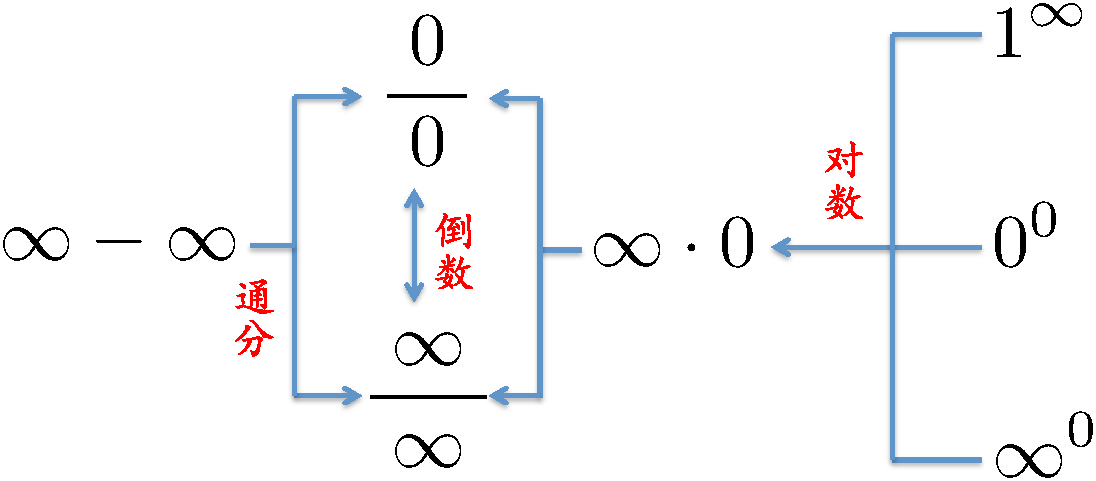
\includegraphics{./images/ch5/lim00.pdf}}
\end{center}

既然不定式极限之间存在这样的转换关系,理论上讲,只要解决了其中的一类问题,则可以将
有关的结果直接推广应用于其他的类型,或者说,总可以将任何一类不定式的问题化为其中的
一个类型(例如$\df{\bm0}{\bm0}$型)的极限来讨论。正因为如此,才有了所谓无穷小
的比较这一说法。

\begin{thx}
	设$\alpha,\beta$均为$x\to\Delta$时的无穷小,且
	$\limx{\Delta}\df{\beta}{\alpha}=A$
	\begin{enumerate}[(1)]
% 	  \setlength{\itemindent}{1cm}
	  \item $A=0$,称$\beta$为$\alpha$当$x\to\Delta$时的{\bf 高阶(高级)无穷小},
	  记为:
	  $$\beta=\circ(\alpha)\;\;(x\to\Delta)$$
	  \begin{itemize}
	    \item {\bf 无穷小}可记为:
	    $\beta=\circ(1),\alpha=\circ(1)\;\;(x\to\Delta)$
	  \end{itemize}
	  \item $A\ne 0$,称$\beta$为$\alpha$当$x\to\Delta$时的{\bf 同阶(同级)无穷小},记为:
	  $$\beta=\mathrm{O}(\alpha)\;\;(x\to\Delta)$$
	  \item $A=1$,称$\beta$为$\alpha$当$x\to\Delta$时的{\bf 等价无穷小},记为:
	  $$\beta\sim \alpha\;\;(x\to\Delta)$$
	\end{enumerate}
\end{thx}
{\bf 注:}在等式中出现无穷小符号$\circ$或$\mathrm{O}$时,等号的含义,准确地
解释应该是指左侧函数为右侧符号所标识的函数之一!因为这样的函数有远远不止一个!

另外,所有的无穷小都必须是和某个$x\to\Delta$相关的,因此讨论
无穷小性质或者对其进行计算、推导时,必须说明是在怎样的$x$变化趋势之中!!!

\begin{shaded}
	{\bf 高阶无穷小的演算}
	
	对包含有无穷小符号的表达式进行推导,不可避免地会涉及一些化简、合并运算,以下是一些常用
	的化简形式,以$x\to 0$时的无穷小为例:
	\begin{tcolorbox}
		\begin{enumerate}[(1)]
% 	  	  \setlength{\itemindent}{1cm}
	  	  \item $C\cdot\circ(x^n)=\circ(x^n)\;(C\in\mathbb{R}\mbox{为常数})$
		  \item $x^n=\circ(x^m)\quad (m<n)$ 
		  \item $\circ(x^n)=x^n\cdot\circ(1)$
		  \item $\circ(x^n)\pm\circ(x^n)=\circ(x^n)$
		  \item $x^n\cdot\circ(x^m)=\circ(x^{m+n})$ 
		  \item $\circ(x^n)+\circ(x^m)=\circ(x^n)\;(m\geq n)$  
		  \item $\circ(x^n)\cdot\circ(x^m)=\circ(x^{m+n})$
		\end{enumerate}
	\end{tcolorbox}
	要正确理解以上的表达式,必须注意到其中的等号的意义与我们惯常使用的有所不同,其含义
	不是指表达式两边恒等,而应该理解成类似集合运算中的属于关系,例如:$x^n=\circ(x^m)\quad (m<n)$ 
	应该理解为$x_n$是所有$x^m$的高阶无穷小中的一个(属于$\circ(x^m)$所标识的一族函数);
	$x^n\cdot\circ(x^m)=\circ(x^{m+n})$应该理解为,一个$x^m$的高阶无穷小,乘以
	$x^n$,所得函数是$x^{m+n}$的一个高阶无穷小中(属于$\circ(x^{m+n})$所标识的
	一族函数)。事实上,所有包含了高阶无穷小的等式,其中的等号都应该做类似的理解!
	
	在今后的极限计算中,我们可能会用到Taylor展开式,例如:
	\begin{align}
		\limx{0}\df{e^{x^2}-\cos x}{x^2}&=\limx{0}
		\df{1+x^2+\circ(x^2)-1+\df{x^2}2+\circ(x^2)}{x^2}\notag\\
		&=\limx{0}\df{\df32x^2+\circ(x^2)}{x^2}=\df32\notag
	\end{align}
\end{shaded}

% \subsection{(等价)无穷小代换}

不难证明,等价无穷小具有如下的一些性质:
\begin{itemize}
  \setlength{\itemindent}{1cm}
  \item $\beta\sim\alpha\Leftrightarrow\beta=\alpha+\circ(\alpha)$,或者
	$\alpha=\beta+\circ(\beta)$;
  \item {\it 自反性:} $y\sim y$ ;
  \item {\it 对称性:} $y_1\sim y_2\Rightarrow y_2\sim y_1$; 
  \item {\it 传递性:} $y_1\sim y_2,y_2\sim y_3\Rightarrow y_1\sim y_3$。 
\end{itemize}

由它们,进一步可以得到如下关于等价无穷小代换的定理:

\begin{thx}
	{\bf 无穷小代换定理:}设$\alpha\sim \beta\;(x\to\Delta)$,则
	$$\limx{\Delta}\alpha\gamma=A
	\quad\Leftrightarrow\quad\limx{\Delta}\beta\gamma=A.$$
\end{thx}

这个定理意味着,极限“{\it 乘法因子}”中的等价无穷小可相互替代,这对于我们简化极限运算会大有帮助。
例如:当$x\to 0$时,我们有$\sin x\sim x$且$1-\cos x\sim\df12x^2$,故
$$\limx0\df{\sin x^2}{1-\cos x}=\limx0\df{x^2}{\frac{x^2}2}=2.$$

{\bf 问:}如果不是乘法因子,这样的代换还能正确进行吗?

[答]:不能保证结果的正确!例如极限$\limx0\df{\tan x-\sin x}{x^3}$。

如果直接进行代换,由$\tan x\sim x,\sin x\sim x$,可得
$$\limx0\df{\tan x-\sin x}{x^3}=\limx0\df{x-x}{x^3}=0.$$
但是,正确的结果应该是这样的:
$$
	\limx0\df{\tan x-\sin x}{x^3}
	=\limx0\df{\sin x(1-\cos x)}{x^3\cos x}
	=\limx0\df{x\frac{x^2}2}{x^3\cos x}
	=\limx0\df1{2\cos x}=\df12.
$$

\begin{thx}
	一些常用的等价无穷小:$x\to 0$时,
	\begin{enumerate}[(1)]
% 	  \setlength{\itemindent}{1cm}
	  \item $x\sim \sin x\sim \tan x$ 
	  \item $x \sim\arcsin x\sim\arctan x$ 
	  \item $1-\cos x\sim \df 12 x^2$ 
	  \item $(1+x)^a-1\sim ax$ 
	  \item $\ln(1+x)\sim x$ 
	  \item $a^x-1\sim x\ln a\;(a>0)$
	\end{enumerate}
\end{thx}

{\bf 例:}利用无穷小代换计算极限
\begin{enumerate}[(1)]
  \setlength{\itemindent}{1cm}
  \item $\limx{0}\df{\arctan x}{\sin 4x}=\limx0\df{4x}x=\df14$; 
  \item $\limx{0}\df{\ln\cos ax}{\ln\cos bx}
  =\limx{0}\df{\ln[1+(\cos ax-1)]}{\ln[1+(\cos bx-1)]}
  =\limx{0}\df{1-\cos ax}{1-\cos bx}
  =\limx{0}\df{\frac12(ax)^2}{\frac12(bx)^2}
  =\df{a^2}{b^2}$;
  \item $\limx{0}\df{\cos x(e^{\sin x}-1)^4}{\sin^2 x(1-\cos x)}
  =\limx0\df{\cos x(\sin x)^4}{x^2\frac12x^2}
  =\limx0\df{\cos x x^4}{\frac12x^4} =2$; 
  \item $\limx{0}\df{\sin x-\tan x}{x^3}
  =\limx{0}\df{\sin x(\cos x-1)}{x^3\cos  x}
  =\limx{0}\df{-x\frac12x^2}{x^3\cos  x}=-\df12$;
  \item $\limx0\df{e^{\sin2x}-e^{2\sin x}}{x^2\ln(1+x)}
  =\limx0\df{e^{2\sin x}[e^{2\sin x(\cos x-1)}]}{x^3}
  =\limx0\df{2\sin x(\cos x-1)}{x^3}=-1.
  $
\end{enumerate}

{\bf 例:}若$x\to 0$时,$\ln\left(\cos\df{2x}3\right)\sim Ax^k$,则
$A=$\underline{$-\df29$},$k=$\underline{$2$}

[提示]:$x\to 0$时,
$$\ln\left(\cos\df{2x}3\right)\sim \cos\df{2x}3-1
\sim-\df12\left(\df{2x}3\right)^2=-\df29x^2.$$

{\bf 例:}设$\limn\df{n^a}{n^b-(n-1)^b}=10$,则$a=\underline{-9/10},
b=\underline{1/10}$

[提示]:
$\limn\df{n^a}{n^b-(n-1)^b}=10=\limn\df{n^{a-b}}{1-\left(1-\df1n\right)^b}
=\limn\df{n^{a-b+1}}b,$
由此可知,显然$b\ne 0$,且只有当$a-b+1=0$时,极限为为零有限值。

熟练掌握和应用等价无穷小代换,能够使我们在计算极限值时获得很大的便利,但是必须指出的是,
到目前为止,还存在相当多的极限问题是我们无法求解的,例如:
$$\limx0\df{x-\sin x}{x^3},
\quad\limx{0}x^4{e^{1/x}},$$
这些题目需要我们在后续章节中学习的L'Hospital法则和Taylor公式等新的工具。
特别值得一提的是,学习完Taylor公式后,我们将会对无穷小的认识有一个大大深入的理解和认识。

\begin{ext}
	{\centering\bf 课后作业}
	
	\begin{enumerate}  
	  \item 计算下列极限
	  \begin{enumerate}[(1)]
% 	    \item $\limx{+\infty}(\sqrt{x^2+x+1}-\sqrt{x^2+x-1})$ 
%   		\item $\limx{0}\df{\sqrt[3]{1+x}-1}{x}$ 
		\item $\limx{0}\df{\sqrt{1-\cos x^2}}{1-\cos x}$ 
		\item $\limx{0}\df{1-\cos x\cos 2x}{1-\cos x}$
		\item $\limx{\pi /4}(\tan x)^{\tan 2x}$ 
		\item $\limx{0}\left(2e^{\frac{x}{x+1}}-1\right)^{\frac{x^2+1}{x}}$ 
		\item $\limx{+\infty}\left(\sqrt{x^2+x}-\sqrt[3]{x^3+x^2}\right)$ 
% 		\item $\limx{+\infty}\left(\df{x^2-1}{x^2+1}\right)^{x^2}$
		\item $\limx{0}\left(\df{a^x+b^x+c^x}{3}\right)^{1/x}\,(a,b,c>0)$  
		\item $\limx0\df{\sqrt[n]{1+\sin x}-1}{\tan x}$
		\item $\limx0(x+e^x)^{\frac1x}$
	  \end{enumerate}
	  \item 求下列函数的渐近线方程(包括:水平、铅直和斜渐近线)
	  \begin{enumerate}[(1)]
	    \item $y=\sqrt{1+x^2}-x$;
	    \item $y=(x+6)e^{\frac1x}$。
	  \end{enumerate}
	  \item 已知$\limx{\infty}\left(\df{x+1}{x+k}\right)^x
	  =\limx0e^{\frac{\sin 4x}x}$,求$k$的值。
	  \item 设$\limx0\df{\ln\left(1+\df{f(x)}{\sin x}\right)}{a^x-1}=A\;(a\ne 1)$,求
		$\limx0\df{f(x)}{x^2}$。
	\end{enumerate}
	\tcblower
	{\kaishu\b 以下各题选作:}
	
	计算下列极限:
	\begin{enumerate}[(1)]
		\item $\limx0\left(\df{e^x+xe^x}{e^x-1}-\df1x\right)$
		\item $\limx0\df1{x^3}\left[\left(\df{2+\cos x}3\right)^x-1\right]$
		\item $\limn\ln\left(\df{n-2na+1}{n(1-2a)}\right)^n\quad(a\ne1/2)$
		\item $\limx0\df{[\sin-\sin(\sin x)]\sin x}{x^4}$
		\item $\limx0\df{e^{\tan x}-e^{\sin x}}{x\sin^2x}$
		\item $\limx0\df{\sqrt{1+\tan x}-\sqrt{1+\sin x}}{x(1-\cos x)}$
		\item $\limn\left(n\tan\df1n\right)^{n^2}$
		\item $\limx0\df{\sin x+x^2\sin\df1x}{(1+\cos x)\ln(1+x)}$
		\item $\limx0\left[\df
		  ax-\left(\df1{x^2}-a^2\right)\ln(1+ax)\right]$\quad($a\ne 0$)
		\item $\limx{0}\left(\df{a^{x+1}+b^{x+1}+c^{x+1}}{a+b+c}\right)^{1/x}
		  \,(a,b,c>0)$
		\item $\limx{0}\df{\tan(\tan x)-\sin(\sin x)}{\tan x-\sin x}$ 
		\item $\limx{\infty}\df{(x+a)^{x+a}(x+b)^{x+b}}{(x+a+b)^{2x+a+b}}$
		\item $\limx{0^+}\df{x^x-(\sin x)^x}{x^2\ln(1+x)}$
		\item $\limx0\df{\cos x-e^{-\frac{x^2}2}}{x^2[x+\ln(1-x)]}$
		\item $\limx{+\infty}\left(x+e^x\right)^{\frac1x}$
		\item $\limx{+\infty}\left(x+\sqrt{1+x^2}\right)^{\frac1x}$
		\item $\limx0\df{\sin x-x\cos x}{\sin^3x}$
		\item $\limx{+\infty}\df{e^x}{\left(1+\df1x\right)^{x^2}}$
		\item $\limx0\df{\ln(\sin^2x+e^x)-x}{\ln(x^2+e^{2x})-2x}$
		\item $\limx1\df{x-x^x}{1-x+\ln x}$
		\item $\limx0\df{1-\cos x\sqrt{\cos2x}}{x^2}$
		\item $\limx{0^+}\df{\ln(1+e^{\frac2x})}{\ln(1+e^{\frac1x})}$
		\item $\limx{+\infty}\df{e^x-e^{-x}}{e^x+e^{-x}}$
		\item $\limx0\left(\df1n\sum\limits_{k=1}^na_k^x\right)^{\frac1x}
		  \quad (a_k>0,k=1,2,\ldots,n)$
		\item $\limn n^2\left(\arctan\df an-\arctan\df a{n+1}\right)\quad (a>0)$
		\item $\limx0\df{(1+x)^{\frac1x}-(1+2x)^{\frac1{2x}}}{\sin x}$
		\item $\limn\left[\left(n^3-n^2+\df n2\right)e^{\frac1n}-\sqrt{1+n^6}\right]$
	  \end{enumerate}
\end{ext}

\section{函数的连续性}

\subsection{函数连续的概念}

\begin{thx}
{\bf 函数$f(x)$在$x_0$连续},也即:
	$$\limx{x_0}f(x)=f(x_0).$$
\end{thx}
如果记$\Delta y=f(x_0+\Delta x)-f(x_0)$,则函数连续也可以等价地表示为:
$$\b\lim\limits_{\Delta x\to 0}\Delta y=0.$$

直观地理解,就是在$x_0$左右两侧的函数值都趋于相同的极限(左右极限相等),
且极限值恰好是这一点处的函数值。因此,函数连续也等价于
\begin{itemize}
  \setlength{\itemindent}{1cm}
  \item $f(x)$在$x_0$有定义; 
  \item $\limx{x_0}f(x)$存在; 
  \item $f(x_0)=f(x_0+0)=f(x_0-0)$。
\end{itemize}
以上三者都是函数连续的必要条件。

从代数运算的意义上,函数连续等价于该函数的运算可以和极限运算交换次序,因为
连续的定义事实上也可以写为:
$$\b\limx{x_0}f(x)=f(\limx{x_0}x).$$

{\bf 注:}必要时,可以只考虑函数在某点一侧的连续性,即所谓{\it 左(右)连续}。

{\bf 例:}证明:$f(x)=xD(x)$只在$x=0$处连续。
\ps{在现实世界里,没有只在一个点连续的曲线,这是数学概念和直观现实存在差异的一个很好的例证}

[提示]:先证明$xD(x)$仅在$x=0$处极限存在。

{\bf 例:}
设$f(x)$在$(-\infty,+\infty)$上有定义,
且对任意$x,y\in (-\infty,+\infty)$,有
$$f(x+y)=f(x)+f(y),$$
则$f(x)$在$(-\infty,+\infty)$上连续,当且仅当$f(x)$在$x=0$连续。

[证]:在已知等式中同时令$x=y=0$,可得$f(0)=0$。

对任意$x_0,\Delta x\in\mathbb{R}$,由已知
$$f(x_0+\Delta x)=f(x_0)+f(\Delta x).$$
由连续的定义,$f(x)$在$x_0$连续,当且仅当
$$\lim\limits_{\Delta x\to 0}f(x_0+\Delta x)=f(x_0),$$
等价于
$$\lim\limits_{\Delta x\to 0}f(\Delta x)
=\lim\limits_{\Delta x\to 0}f(x_0+\Delta x)-f(x_0)=0=f(0),$$
即证。\hfill$\Box$


\subsection{函数的间断点}

{\bf 间断点}即不连续点,根据前述函数连续的必要条件,可以对间断点作出如下的分类:

设$x_0$是$f(x)$的间断点(不连续点),对其分类定义如下:
\ps{此处的第一类、第二类间断点的分类,沿用了KD教材的定义}
\begin{enumerate}[(1)]
  \setlength{\itemindent}{1cm}
  \item {\bf 第一类间断点:}$f(x_0+0),f(x_0-0)$均存在
  \begin{itemize}
    \item {\bf 跳跃间断点:}$f(x_0+0)\ne f(x_0-0)$,例:$y=[x]$当$x$为整数时
    \begin{center}
		\resizebox{!}{4cm}{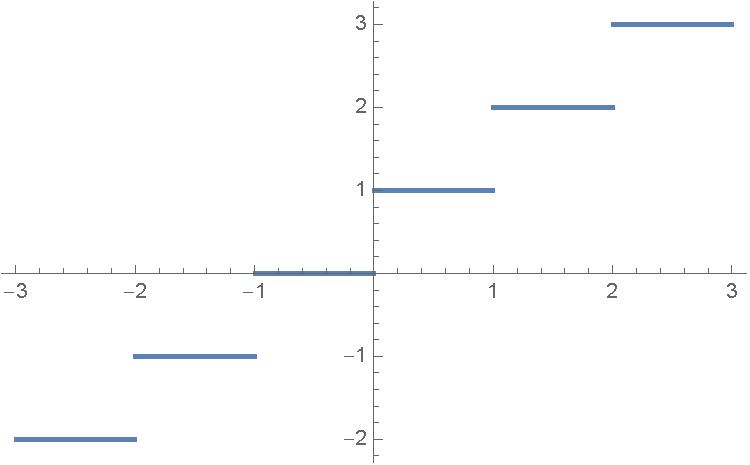
\includegraphics{./images/ch3/roundx.pdf}}
 	\end{center}
    \item {\bf 可去间断点:}$f(x_0)$无定义,或
    $$f(x_0)\ne f(x_0+0)=f(x_0-0)$$
    例:$y=\df{\sin x}x$在$x=0$处
    \begin{center}
		\resizebox{!}{4cm}{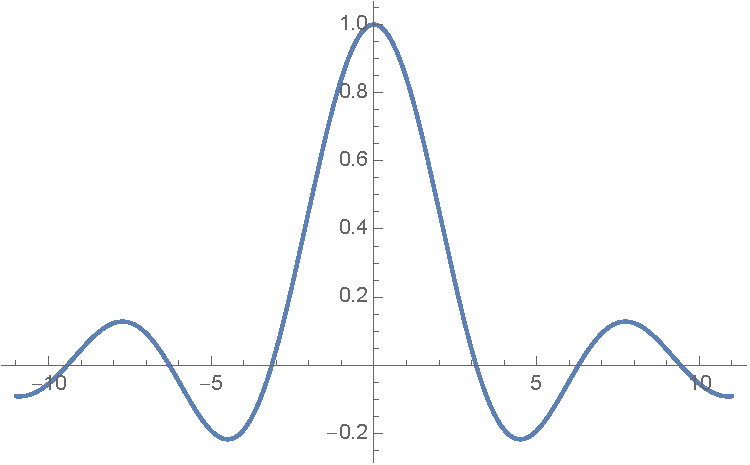
\includegraphics{./images/ch3/sinxox.pdf}}
 	\end{center}
  \end{itemize}
  \item {\bf 第二类间断点:}$f(x_0+0),f(x_0-0)$不同时存在
  \begin{itemize}
    \item {\bf 无穷间断点:}某个单侧极限趋于无穷,例:$y=\tan x$和$y=\sec x$在$x=k\pi+\df{\pi}2$处
     \begin{center}
		\resizebox{!}{4cm}{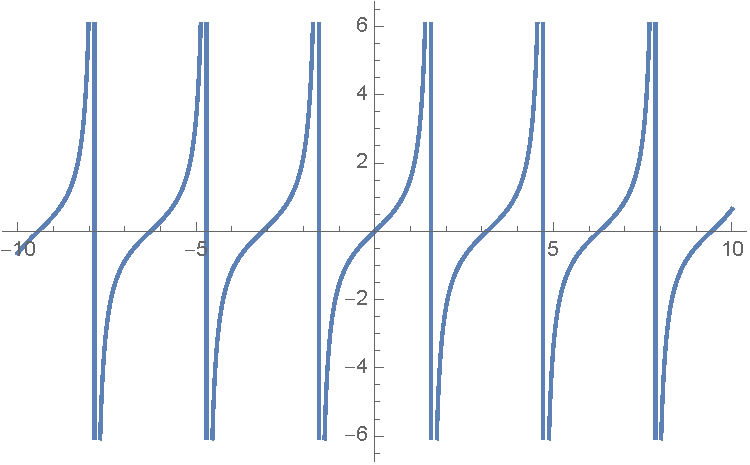
\includegraphics{./images/ch3/tanx.pdf}}
		\resizebox{!}{4cm}{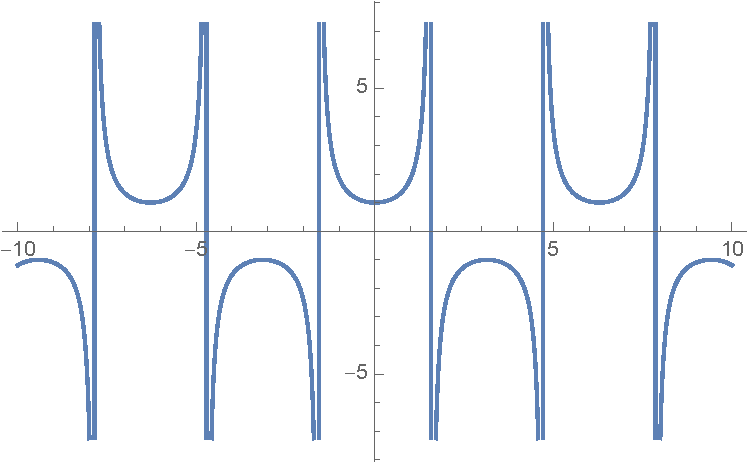
\includegraphics{./images/ch3/secx.pdf}}
 	\end{center}
    \item {\bf 振荡间断点:}某个单侧极限不存在,且非无穷,例:$y=\sin\df1x$在$x=0$处
    \begin{center}
		\resizebox{!}{5cm}{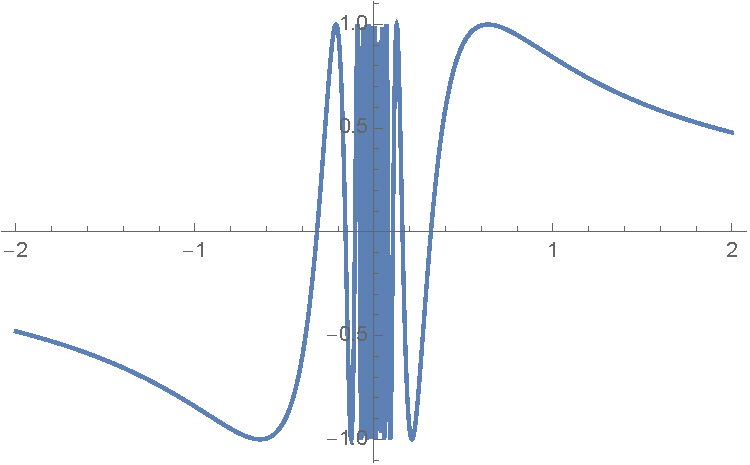
\includegraphics{./images/ch3/sin1ox.pdf}}
 	\end{center}
  \end{itemize}
\end{enumerate}

{\bf 例:}指出以下函数的间断点,判断其类型
\begin{enumerate}[(1)]
  \setlength{\itemindent}{1cm}
  \item $y=\df{x^2-1}{x-1}$\quad{\it 可去}
  \item $y=\df{x^2+1}{x-1}$\quad{\it 无穷}
  \item $y=D(x)$\quad{\it 振荡}
\end{enumerate}

\subsection{连续函数的运算与初等函数的连续性}

\begin{enumerate}[(1)]
  \setlength{\itemindent}{1cm}
  \item {\it 四则运算:} 四则运算仍保持函数的连续性; 
  \item {\it 复合函数:} 连续函数的函数运算可以和极限运算交换次序; 
  \item {\it 反函数:} 连续函数的反函数也连续 ;
  \item {\it 初等函数:} 初等函数在其{\it 定义区间}内连续;
\end{enumerate}

{\bf 注:}以上的定义区间是指函数定义域内的一个开区间,例如:$y=\df1x$在定义域内整体
是不连续的,但在定义域内的任意一个区间内都连续。

\subsection{闭区间上连续函数的性质}

以下我们引入记号$f(x)\in C(I)$,表示函数$f(x)$在区间$I$上连续。例如:
{\b$f(x)\in C[a,b]$表示函数$f(x)$在闭区间$[a,b]$上连续}。

闭区间上的连续函数有一些“有趣”的性质,这些性质在很大程度上是符合我们对
连续这一概念的直观印象的。

\subsubsection{有界性与最值存在性}

\begin{thx}
	{\bf 最值定理:}$f(x)\in C[a,b]$,则$f(x)$在$[a,b]$上可取到最大和最小值。
	{\it 也即,存在$\xi,\eta\in[a,b]$,是对任意$x\in[a,b]$,总有$f(\xi)
	\leq f(x)\leq f(\eta)$}
\end{thx}

此定理掌握结论即可,无须了解证明。下面的推论是显然的

\begin{thx}
	{\bf 有界性:}$f(x)\in C[a,b]$,则$f(x)$在$[a,b]$上有界。
\end{thx}
在闭区间上,连续可以推出有界,但反之不然,请自行思考反例。

利用这一性质,可以证明类似下面的结论:

{\bf 例:}设$f(x)\in C[a,+\infty)$,且$\limx{+\infty}f(x)$存在,
证明:$f(x)$在$[a,+\infty)$上有界。

[提示]:首先利用函数极限的有界性证明,存在$M_1$和$X$,对任意$x>X$,有$|f(x)|<M_1$。
然后,利用连续函数在闭区间上的有界性,说明存在$M_2$,对任意$x\in[a,X]$,有$|f(x)|<M_2$。
综合即证。

\subsubsection{介值定理和零点存在定理}

\begin{thx}
	{\bf 介值定理:}设$f(x)\in C[a,b]$,$M,m$分别为$f(x)$在$[a,b]$上的最大和最小值,
	则对任意$\gamma\in[m,M]$,存在(至少一个)
	$\xi\in[a,b]$,使得$f(\xi)=\gamma$。
\end{thx}

定理证明不需要掌握,略过。该定理最常用的是如下的推论:

\begin{thx}
	{\bf 零值存在定理:}设$f(x)\in C[a,b]$,且$f(a)f(b)<0$,
	则$f(x)$在$[a,b]$上必有零点。
\end{thx}

和前述关于有界性的讨论类似,零点存在定理也可以进一步作如下的推广:
\begin{enumerate}[(1)]
  \setlength{\itemindent}{1cm}
  \item {\b 设$f(x)\in C(a,b)$,且$f(a+0)\cdot f(b-0)<0$,则$f(x)$在$(a,b)$内有零点。} 
  \item {\b 设$f(x)\in C(-\infty,+\infty)$,且$f(-\infty)\cdot f(+\infty)<0$,
  则$f(x)$在$(-\infty,+\infty)$内有零点。}
\end{enumerate}

[提示]:利用极限的保号性证明。

{\bf 例:}设$a_0\ne 0$,证明:以下方程至少有一个实根\ps{\b 奇数次多项式方程至少有一个实根!}
$$a_0x^{2n+1}+a_1x^{2n}+\ldots+a_{2n}x+a_{2n+1}=0.$$

[提示]:$\limx{\infty}\df{f(x)}{x^{2n+1}}=a_0$,利用极限保号性说明
$f(x)$当$x$充分大(小)时,分别有取正和取负的值。

{\bf 例:}已知$f(x)\in C[0,3]$,且$f(0)=f(3)$,证明:至少存在
一个$\xi\in[0,2]$,使得$f(\xi+1)=f(\xi)$

[证]:设$F(x)=f(x+1)-f(x)$,显然$F(x)\in C[0,2]$。

注意到若$f(0)=f(1)$或$f(1)=f(2)$或$f(2)=f(3)$,结论显然成立。故以下设$f(0)\ne f(1),
f(1)\ne f(2),f(2)\ne f(3)$。

不妨设$f(1)>f(0)$,则$F(0)>0$。此时,若$f(2)<f(1)$,则$F(1)<0$,
由连续函数的介值定理可知必有$\xi\in[0,1]$,使得$F(\xi)=0$。
又若$f(2)>f(1)$,则$F(1)>0$,
$$F(2)=f(3)-f(2)=f(0)-f(2)<f(1)-f(2)=-F(1)<0,$$
同样由连续函数的介值定理可知必有$\xi\in[1,2]$,
使得$F(\xi)=0$。

综上,必有$\xi\in[0,2]$,使得$F(\xi)=0$,也即$f(\xi+1)=f(\xi)$。\hfill $\Box$

{\bf 例:}设$G$是第一象限内的一个有界区域(其边界为连续的简单闭曲线),$ABCD$表示
它的一个外接矩形。矩形的一条边与$x$轴的夹角记为$\theta$,如果对于任意$\theta\in
[0,\pi/2]$,$G$总可以被某个外接矩形所围,证明:至少存在某个$\theta_0\in[0,\pi/2]$,
使得与之对应的外接矩形恰好为正方形。({\it 推论:任一平面有界区域都可以内接于某个正方形})

\begin{center}
	\resizebox{!}{6cm}{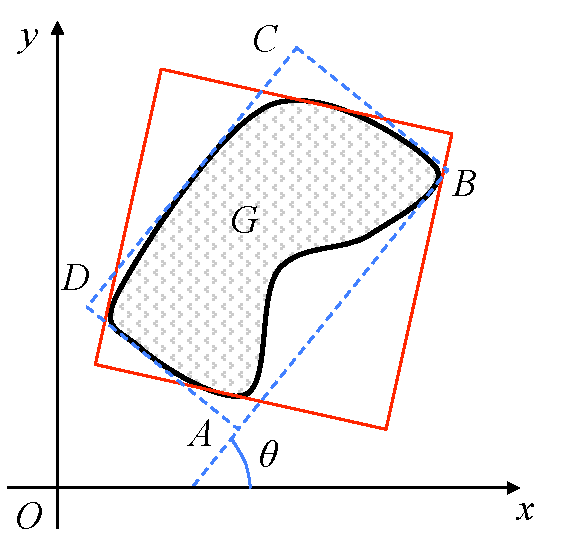
\includegraphics{./images/ch3/sqOut.pdf}}
\end{center}

[提示]:如图,记$l_1(\theta),l_2(\theta)$分别为$AB$和$BC$的长度,显然
$$l_1(0)=l_2(\pi/2),\quad l_2(0)=l_1(\pi/2).$$
令$f(\theta)=l_1(\theta)-l_2(\theta)$,由介值定理可以证明$f(\theta)$存在零点。

{\bf 例:}证明:给定任意平面有界区域,以及一个向量,一定存在一条与该向量平行的直线
平分该区域。

{\bf 例:}证明:给定任意平面有界区域,一定存在两条相互垂直的直线,将其四等分。

[证]:设其中一条直线的极角为$\theta$,则另一条的为$\theta+\pi/2$。
分别记两条直线为$l_{\theta}$和$l_{\theta+\pi/2}$,显然可以使得二者都平分给定区域。
设此时四个区域的面积按顺时针方向依次为$S_1,S_2,S_3,S_4$,且由平分可满足
$$A_1+A_2=A_3+A_4,\quad A_1+A_4=A2+A_3,$$

\begin{center}
	\resizebox{!}{6cm}{\includegraphics{./images/ch3/4cut.pdf}}
\end{center}

由此可得
$$A_1=A_3,\quad A_2=A_4.$$
进而,只需适当取$\theta$,使得$A_1=A_2$即可。

记$f(\theta)=A_1(\theta)-A_2(\theta)$,不妨设$f(0)>0$,从而
$$f(\pi/2)=A_1(\pi/2)-A_2(\pi/2)=A_4(0)-A_1(0)=A_2(0)-A_1(0)=-f(0)<0,$$
由介值定理,即证。\hfill$\Box$

{\bf 例:}任意金属圆环上,总存在相对的两点温度相同。

如果将地球的赤道看成圆环,以上结论告诉我们:必有赤道上相对的两点温度恰好相同。

[提示]:默认假设温度总是连续分布的。

{\bf 例:}一个哨兵头一天下午三点从$A$至$B$巡逻,五点到达;隔天
还是下午三点再从$B$沿原路返回$A$,五点到达。证明:两天中必有一个时刻,
他恰好位于同一个地点。

{\bf 思考:}构造更多类似的例题,用介值定理证明某种状态的存在性。

\begin{ext}
	{\centering\bf 课后作业}
	
	\begin{enumerate}  
	  \item 讨论函数$f(x)=\df1{1-e^{\frac{x}{x-1}}}$的间断点,并说明其类型。
	  \item 试确定常数$a,b$的值,是的函数
	  $$
	  	\left\{\begin{array}{ll}
	  		\df{\ln(1+2x)}x,& x<0,\\
	  		a,& x=0,\\
	  		\df{e^{bx}+bx-1}x,& x>0
	  	\end{array}\right.
	  $$
	  在$x=0$处连续。
	  \item 讨论函数$f(x)=\limn\df{1-e^{nx}}{1+e^{nx}}$的连续性,在
	  不连续处,说明间断点的类型。
	  \item 证明:存在某个实数,其值恰好比它自身的立方少$1$。
	  \item 设$f(x)\in C[a,b]$,且$f(0)=f(1)$,证明:必存在某个
	  $\xi\in\left[0,\df12\right]$,使得$f(\xi)=f\left(\xi+\df12\right)$。
	  (以下选作)能否进一步证明,对任意$n\in\mathbb{Z}^+$,都存在某个
	  $\xi_n\in\left[0,1-\df1n\right]$,使得
	  $f(\xi_n)=f\left(\xi_n+\df1n\right)$。
	  \item (选作)设$f(x)\in C(\mathbb{R})$,且$f(\infty)$存在,
	  证明:$f(x)$在$\mathbb{R}$上有界。
% 	  \begin{enumerate}[(1)]
% 	    \item $\limn\df{\sqrt{n^2+a^2}}n=1$;
% 	    \item $\limn0.\underbrace{999\ldots9}_{n\mbox\footnotesize 个}=1$;
% 	    \item $\limn(\sqrt[3]{n+1}-\sqrt[3]n)=0$.
% 	  \end{enumerate}
	\end{enumerate}
\end{ext}

\section*{小结}
\addcontentsline{toc}{section}{小结}

数列极限是我们研究和讨论更一般的函数极限的基础,因为其典型性和相对简单直观的性质,成为了
我们进入微积分的起始点。

本章的一个难点是{\it 数列极限的“$\e-N$”定义},能够准确叙述定义,并使用其来证明一些极限
对于很多同学来说需要付出巨大的能力。通过这部分的学习,能使大家对什么是严谨的数学和逻辑推理,
怎样作到数学表达的严密和精确有一个初步的体验。

就目前来看,用定义证明数列极限从未作为各级高数考试的重点,这可以说是非常幸运的。
而本章真正的重点,毫无疑问,是数列极限的判敛和计算。我们介绍了一些典型的方法
和常用技巧,包括:{\it 子数列的性质、夹逼定理、单调有界原理、递推数列的判敛、
Stolz定理等}。对所有这些方法的理解和纯熟掌握本章学习的目标之一。

函数极限与数列极限最明显的不同,就是所考虑的自变量变化过程,从单一的趋于正无穷扩展到了
趋于无穷和趋于有限值两大类,共六种不同的过程。

在学习函数极限的概念,或者说“$\e-X$”(“$\e-\delta$”)定义时,一定要注意和数列极限
的“$\e-N$”定义进行类比,严格来说,在所有这些不同极限的定义中,有所变化的只是所趋近的目标
(无穷或有限值)的邻域概念,定义的结构和内涵都是完全一样的,即:{\it 只要自变量充分靠近
趋近的目标,则函数值也会充分靠近某个稳定的值。}

正因文定义上的相似,所以在基本的性质上,函数极限和数列极限也没有本质的不同。需要注意
的仅仅是有些性质在表述上的变化,例如{\it 函数极限的有界性}和数列极限的有界性在表述上就存在
明显的差别,能够正确表述函数极限的有界性,是本章学习的第一个有挑战的知识点。

和数列极限一样,本章学习的重点是函数极限的判敛和计算问题,特别是后者。我们所学习的{\it 两个
重要极限和众多由它们衍生的常用极限},是我们今后计算很多极限的基础。在此需要提醒同学们的是,
拿到一个极限问题,首先要判断其基本的形态(例如:“$0/0$”,“$1^{\infty}$”),然后
根据其形态上的特点选择运算的方向(或者说变换的目标),最终将其化为一些我们常见或者说
基本的极限。这一点,常常被很多同学所忽视。

无穷小的概念是微积分真正成为一门新学科,在数学理论中确立其独特地位的源头。Newton最早
有意识地使用了无穷小的概念,并利用其种种性质达到简化计算和推理的目的,但无穷小的有关理论是在
其诞生后近百年后才真正稳固的。也正因为如此,无穷小也是本章学习的难点和重点。所谓的难点,
主要体现在对无穷小的“运算”方法(例如:$\circ(x^2)+\circ(x)=\circ(x)$)的理解,以及
何时可以在有关的计算(不仅仅是极限问题)中准确地将其忽略不计。至于其重要性可以说是不言而喻
的,{\it 无穷小代换}的思想对于我们计算各种不定式的极限给出了崭新的思路和表述方法,极大提高了
极限计算的效率。在本章之外,无穷小的故事还会继续。

函数的连续性概念源于生活的直觉,但并不等同于直觉,事实上,在现实中就没有“在某一点连续”
的直觉对应。{\it 函数连续的本质是,函数运算和极限运算可以交换次序},换句话说,对于在某点连续的
函数而言,计算其在该点的极限和计算其函数值没有什么不同。

{\it 有界闭区间上连续函数的性质}是本章最富有趣味也是颇具挑战性的问题,特别是和我们后续
学习中的中值定理相结合,将展示给大家极为丰富和多样化的挑战性问题,并成为本门课程的又一个
标志性的难点。

% \newpage

% \section*{课后作业}
% \addcontentsline{toc}{section}{课后作业}
% % {\bf 【必作题】}
% {\b\it 说明:作业必须写明题目所在章节、页码、题号;如非特别说明,
% 所有题目必须抄题;两道题之间空一行;未作或作错的题目讲评后务必及时订正。}
% 
% \begin{itemize}
%   \item 注册加入课程网站:https://www.trustie.net/courses/1259,邀请码:YRKWF
%   \item 注册中学大学MOOC账号:http://www.icourses.cn/imooc/,将用户名告知课代表
%   统一登记
%   
%   {\b\it 下面的题目请写在活页纸上,不用抄题:}
%   \item 写一篇短文,内容及要求如下
%   \begin{enumerate}[(1)]
%     \item 你的个人介绍,请务必包含如下信息:姓名、性别、年龄、籍贯、中学母校的名字、
%     你的高考总成绩(以及当地的满分)、你的高考数学成绩(以及当地的满分);
%     \item 你的兴趣爱好、特长,或者说,你觉得自己有什么与众不同之处;
%     \item 你学习数学的体会,例如:喜欢,不喜欢?喜欢什么样的数学,不喜欢什么样的数学?
%     有什么好的学习方法?有什么自己觉得成功的经验,或者有趣的经历(最好与数学有关)?
%     \item 你期待中的大学课堂是怎样的?怎么的教与学会对你更有帮助?对老师有什么期待、要求,
%     或者建议?
%     \item 请至少推荐一本(部、套)你喜欢的书、电影或者其他任何可以通过公共渠道获取到的资料
%     (例如:网站、软件、APP、\ldots),说说推荐的理由;
%     \item 其他任何你认为值得(可以)与我交流的东西,比如你想问我什么问题;
%     \item 除第一条必须包含外,其余内容可自由取舍。
%     \item 篇幅:不少于半页,不多于两页(一张纸的正反面)。
%   \end{enumerate}
%   {\b\it 以下的题目写在作业本上,作业本第一页背面上贴上一张个人的照片,标注专业和籍贯}
%   \item 习题1-2:5(3,4),7,8
%   \item 习题1-3:5(3),6(2),7,8
%   \item 习题1-4:7,8
%   \item 习题1-5:3
%   \item 习题1-6:4(2,3,5)
%   \item 习题1-7:4(2),5(3,4)
%   \item 习题1-8:4
%   \item 习题1-9:2,3(3,5,6),4
%   \item 习题1-10:1,5,7
%   \item 总习题一:14
% \end{itemize}

% \bigskip
% 
% \hrule
% 
% \bigskip
% \bigskip
% 
% {\bf 【思考题】}\ps{\b 思考题主要作为课后的辅助阅读,欢迎课间找我讨论,不必写在作业纸上}
% 
% \begin{itemize}
% %   \item 习题1.1:(C)应用题
%   \item 习题1.2:13,17,22,23
%   \item 习题1.3:6,7,9
%   \item 习题5.2:3
%   \item 阅读:李开复,《给未来的你》
% \end{itemize}

\newpage

\section*{作业参考解答}
% \addcontentsline{toc}{section}{作业参考解答}

\begin{center}
	\bf 习题1-2
\end{center}

5.用数列极限的定义证明

(1)$\limn\df{\sqrt{n^2+a^2}}n=1$;

[证]:对任意$\e>0$,令$N=\left[\df{a^2}{\e}\right]+1>\df{a^2}{\e}$,
则对任意$n>N$,均有
$$\left|\df{\sqrt{n^2+a^2}}n-1\right|
=\df{a^2}{n(\sqrt{n^2+a^2}+n)}<\df{a^2}n<\df{a^2}N<\e,
$$
由数列极限的定义,即证。\hfill$\Box$

\bigskip

(4)$\limn0.\underbrace{99\ldots9}_{n\mbox{\footnotesize 个}}=1.$

[证]:对任意$\e>0$,令$N=[-\lg\e]+1$,则对任意$n>N$,均有
$$|0.\underbrace{99\ldots9}_{n\mbox{\footnotesize 个}}-1|
=\df1{10^n}<\df1{10^N}
<\df1{10^{-\lg\e}}=\e,$$
由数列极限的定义,即证。\hfill$\Box$

\bigskip

7.数列$\{x_n\}$有界,$\limn y_n=0$,证明:$\limn x_ny_n=0$。

[证]:数列$\{x_n\}$有界,故存在$M>0$,对任意$n\in\mathbb{Z}_+$,均有
$$|x_n|\leq M.$$
对任意$\e>0$,令$\e_1=\df{\e}M$,由$\limn y_n=0$,存在$N$,对任意$n>N$有
$$|y_n-0|<\e_1.$$
综上,当$n>N$时,总有
$$|x_ny_n-0|\leq M\e_1=\e,$$
由数列极限的定义,即证。\hfill$\Box$

\bigskip

8.对于数列$\{x_n\}$,若$x_{2k-1}\to a\,(k\to\infty)$,
$x_{2k}\to a\,(k\to\infty)$,证明:
$x_n\to a\,(n\to\infty)$。

[证]:对任意$\e>0$,由$x_{2k-1}\to a\,(k\to\infty)$,存在$K_1$,
对任意$k>K_1$,有$|x_{2k-1}-a|<\e$;

对以上的$\e>0$,由$x_{2k}\to a\,(k\to\infty)$,存在$K_2$,
对任意$k>K_2$,有$|x_{2k}-a|<\e$。

综上,令$N=\max\{2K_1-1,2K_2\}$,则对任意$n>N$,均有
$$|a_n-a|<\e.$$
由数列极限的定义,即证。\hfill$\Box$

\bigskip

\begin{center}
	\bf 习题1-3
\end{center}

5.根据函数极限的定义证明:

(3)$\limx{-2}\df{x^2-4}{x+2}=-4$.

[证]:对任意$\e>0$,令$\delta=\e$,则对任意$x\in U_0(-2,\delta)$,总有
$$\left|\df{x^2-4}{x+2}-(-4)\right|=|x+2|<\delta=\e.$$
由函数极限的定义,即证。\hfill$\Box$

\bigskip

6.根据函数极限的定义证明:

(2)$\limx{+\infty}\df{\sin x}{\sqrt x}$.

[证]:对任意$\e>0$,令$X=\df1{\e^2}$,则对任意$x>X$,总有
$$\left|\df{\sin x}{\sqrt x}-0\right|\leq\df1{\sqrt x}
<\df1{\sqrt X}=\e.$$
由函数极限的定义,即证。\hfill$\Box$

\bigskip

7.当$x\to2$时,$y=x^2\to 4$,问$\delta$等于多少,使当$|x-2|<\delta$时,
$|y-4|<0.001$?

[解]:
$$|y-4|<0.001\quad\Leftrightarrow\quad 3.999<x^2<4.001.$$
进而当$x>0$时,必有
$$\sqrt{3.999}<x<\sqrt{4.001}.$$
由此可知须
$$|x-2|<\min\{2-\sqrt{3.999},\sqrt{4.001}-2\}$$
时,方能满足题目要求。注意到$2-\sqrt{3.999}>\sqrt{4.001}-2$,故
取$\delta=\sqrt{4.001}-2$,即为所求。\hfill$\Box$

\bigskip

8.当$x\to\infty$时,$y=\df{x^2-1}{x^2+3}\to1$,问$X$等于多少,使当
$|x|>X$时,$|y-1|<0.01$?

[解]:由题意
$$|y-1|=\left|\df{x^2-1}{x^2+3}-1\right|=\df4{x^2+3}<0.01,$$
由此可解得$|x|>\sqrt{397}$,故$X=\sqrt{397}$即为所求。\hfill$\Box$

\bigskip

\begin{center}
	\bf 习题1-4
\end{center}

7.证明:函数$y=\df1x\sin\df1x$在区间$(0,1]$内无界,但不是$x\to0^+$
时的无穷大。

[证]:先证该函数无界。对任意$M>0$,总可令$x_M=\df1{2([M]+1)\pi+\frac{\pi}2}$,
则
$$y(x_M)=\left(2([M]+1)\pi+\frac{\pi}2\right)\sin(2([M]+1)\pi+\frac{\pi}2)
=2([M]+1)\pi+\frac{\pi}2>M.$$
由函数无界的定义,即证。

下证该函数不是$x\to0^+$时的无穷大。用反证法,若该函数是$x\to0^+$时的
无穷大,则
$$\limx{0^+}\df1y=\limx{0^+}x\df1{\sin\frac1x}=0.$$
考虑数列$x_n=\frac1{n\pi}$,显然$\limn x_n=0$,且$\sin\df1{x_n}=0$,
此时$\df1{y(x_n)}$无定义,故$\left\{\df1{y(x_n)}\right\}$
必不收敛,从而由Henie定理,前述极限不成立,
假设错误,即证。\hfill$\Box$

\bigskip

8.求函数$f(x)=\df4{2-x^2}$的渐近线。

[解]:由$\limx{\pm\sqrt 2}\df1{f(x)}=\df{2-x^2}4=0$,可知$f(x)$
是$x\to\pm\sqrt2$时的无穷大,故$x=\pm\sqrt2$为$f(x)$的两条铅直渐近线;

又显然$\limx{\infty}f(x)=0$,故$y=0$是$f(x)$的水平渐近线。\hfill$\Box$

\bigskip

\begin{center}
	\bf 习题1-5
\end{center}

3.计算下列极限:

(1)$\limx0x^2\sin\df1x$

[解]:因为$\limx0x^2=0$,$\left|\sin\df1x\right|\leq1$,由无穷小的性质(无穷小
乘以有界量仍为无穷小),可知
$$\limx0x^2\sin\df1x=0.$$
\hfill$\Box$

\bigskip

(2)$\limx{\infty}\df{\arctan x}x$

[解]:因为$\limx{\infty}\df1x=0$,$|\arctan x|\leq\df{\pi}2$,故
无穷小的性质,可知
$$\limx{\infty}\df{\arctan x}x=0.$$
\hfill$\Box$

\begin{center}
	\bf 习题1-6
\end{center}

4.利用极限存在准则证明:

(2)$\limn n\left(\df1{n^2+\pi}+\df1{n^2+2\pi}+\ldots
+\df1{n^2+n\pi}\right)=1$.

[证]:注意到
$\df{n^2}{n^2+n\pi}<
n\left(\df1{n^2+\pi}+\df1{n^2+2\pi}+\ldots
+\df1{n^2+n\pi}\right)
<\df{n^2}{n^2+\pi},$
而
$$\limn\df{n^2}{n^2+n\pi}=\limn\df1{1+\frac{\pi}n}
=\df1{1+\limn\frac{\pi}n}=1,$$
$$\limn\df{n^2}{n^2+\pi}=\limn\df1{1+\frac{\pi}{n^2}}
=\df1{1+\limn\frac{\pi}{n^2}}=1,$$
故由夹逼准则,即证。\hfill$\Box$

\bigskip

(3)数列$\sqrt2,\sqrt{2+\sqrt2},\sqrt{2+\sqrt{2+\sqrt2}},\ldots$
极限存在。

[证]:记该数列为$\{a_n\}$。显然$\{a_n\}$单调递增。又$a_1<2$,从而
$$a_2=\sqrt{2+a_1}<\sqrt4=2.$$
假设$a_k<2$,则有
$$a_{k+1}=\sqrt{2+a_k}<\sqrt4=2.$$
从而由数学规范,对任意$n\in\mathbb{Z}_+$均有$a_n<2$。至此可知
$\{a_n\}$单调递增有上界,故必收敛。\hfill$\Box$

\bigskip

(5)$\limx{0^+}x\left[\df1x\right]=1$.

[证]:由取整函数的性质,对任意$x>0$,
$$\df1x-1<\left[\df1x\right]\leq\df1x,$$
于是
$$x\left(\df1x-1\right)<x\left[\df1x\right]\leq 1,$$
显然$\limx{0^+}x\left(\df1x-1\right)=1$,故由夹逼定理,即证。
\hfill$\Box$

\begin{center}
	\bf 习题1-7
\end{center}

\bigskip

4.证明:当$x\to 0$时,有

(2)$\sec x-1\sim\df{x^2}2$.

[证]:
$$\limx{0}\df{\sec x-1}{\frac{x^2}2}
=2\limx0\df{1-\cos x}{x^2\cos x}
=2\limx0\df{1-\cos x}{x^2}\limx0\df1{\cos x}
=2\cdot\df12\cdot1=1,$$
即证。\hfill$\Box$

\bigskip

5.利用等价无穷小的性质,求下列极限:

(3)$\limx0\df{\tan x-\sin x}{\sin^3x}$.

[解]:
$$
	\mbox{原式}
	=\limx0\df{\sin x(1-\cos x)}{x^3\cos x}
	=\limx0\df{x\frac{x^2}2}{x^3}\limx0\df1{\cos x}
	=\df12.
$$
\hfill$\Box$

\bigskip

(4)$\limx0\df{\sin x-\tan x}{(\sqrt[3]{1+x^2}-1)(\sqrt{1+\sin x}-1)}$.

[解]:利用第(3)题的结果
$$
\mbox{原式}=\limx0\df{\frac12\sin^3}{\frac13x^2\cdot\frac12\sin x}
=\df12\limx0\df{x^3}{\frac16x^3}=3.
$$
\hfill$\Box$

\begin{center}
	\bf 习题1-7
\end{center}

\bigskip

4.讨论函数$f(x)=\limn\df{1-x^{2n}}{1+x^{2n}}x$的连续性,若有间断点,判别其类型。

[解]:显然,$|x|=1$时,$f(x)=0$。

当$|x|<1$时,$\limn x^{2n}=0$,故
$$f(x)=\df{1-\limn x^{2n}}{1+\limn x^{2n}}x=-x.$$

当$|x|>1$时,$\limn\df1{x^{2n}}=0$,故
$$f(x)=\limn\df{\frac1{x^{2n}}-1}{\frac1{x^{2n}}+1}x
=\df{\limn\frac1{x^{2n}}-1}{\limn\frac1{x^{2n}}+1}x=x.$$

综上可得
$$
	f(x)=\left\{\begin{array}{ll}
		x,& x<-1;\\
		-x, & -1<x<1, \\
		x, & x>1,\\	
		0, & x=\pm1.	
	\end{array}\right.
$$
容易发现,$x=\pm1$是$f(x)$的跳跃间断点。\hfill$\Box$

\begin{center}
	\bf 习题1-9
\end{center}

\bigskip

2.设函数$f(x)$与$g(x)$在点$x_0$连续,证明函数
$$\varphi(x)=\max\{f(x),g(x)\},\quad
\psi(x)=\min\{f(x),g(x)\}$$
在$x_0$也连续。

[证]:注意到
$$\min\{f(x),g(x)\}=f(x)+g(x)-\max\{f(x),g(x)\},$$
由连续函数的性质易知,若$\max\{f(x),g(x)\}$在$x_0$连续,
$\min\{f(x),g(x)\}$也一定在$x_0$连续。以下证明
$\max\{f(x),g(x)\}$在$x_0$连续即可。

事实上,
$$\max\{f(x),g(x)\}=\df12[f(x)+g(x)+|f(x)-g(x)|],$$
由$f(x),g(x)$在$x_0$连续,易知$f(x)-g(x)$在$x_0$连续,
进而可知$|f(x)-g(x)|$在$x_0$连续,从而由连续函数的性质,
$\max\{f(x),g(x)\}$在$x_0$连续。\hfill$\Box$

\bigskip

3.求下列极限

(3)$\limx{\pi/6}\ln(2\cos2x)$

[解]:
$$\mbox{原式}=\ln(2\cos2\limx{\pi/6}x)
=\ln(2\cos\df{\pi}3)=\ln1=0.$$
\hfill$\Box$

\bigskip

(5)$\limx1\df{\sqrt{5x-4}-\sqrt x}{x-1}$.

[解]:
$$\mbox{原式}=\limx1\df{5x-4-x}{(x-1)(\sqrt{5x-4}+\sqrt x)}
=\limx1\df4{\sqrt{5x-4}+\sqrt x}=2.$$
\hfill$\Box$

\bigskip

(6)$\limx a\df{\sin x-\sin a}{x-a}$.

[解]:
$$\mbox{原式}=\limx a\df{2\sin\frac{x-a}2\cos\frac{x+a}2}{x-a}
=\limx a\df{\sin\frac{x-a}2}{\frac{x-a}2}\limx a\cos\frac{x+a}2
=\cos a.$$
\hfill$\Box$

\bigskip

(8)$\limx0\df{\left(1-\df12x^2\right)^{\frac23}-1}{x\ln(1+x)}$

[解]:
$$\mbox{原式}=\limx0\df{-\frac23\cdot\frac12x^2}{x^2}
=-\df13.$$
\hfill$\Box$

\bigskip

4.求下列极限:

(2)$\limx0\ln\df{\sin x}x$.

[解]:
$$\mbox{原式}=\ln\left(\limx0\df{\sin x}x\right)=\ln1=0.$$
\hfill$\Box$

\bigskip

(4)$\limx0(1+3\tan^2x)^{\cot^2x}$.

[解]:令$y=\tan^2x$
$$\mbox{原式}=\lim\limits_{y\to0}(1+3y)^{\frac1y}
=\lim\limits_{y\to0}\left[(1+3y)^{\frac1{3y}}\right]^3
=\left[\lim\limits_{y\to0}(1+3y)^{\frac1{3y}}\right]^3=e^3.$$
\hfill$\Box$

\bigskip

(5)$\limx{\infty}\left(\df{3+x}{6+x}\right)^{\frac{x-1}2}$.

[解]:
$$\mbox{原式}
=\limx{\infty}\df{\left[\left(1+\df3x\right)^{\frac{x}{3}}\right]
^{{\frac3x}\cdot\frac{x-1}2}}
{\left[\left(1+\df6x\right)^{\frac{x}{6}}\right]
^{{\frac6x}\cdot\frac{x-1}2}}
=\df{\left[\limx{\infty}\left(1+\df3x\right)^{\frac{x}{3}}\right]
^{\limx{\infty}{\frac3x}\cdot\frac{x-1}2}}
{\left[\limx{\infty}\left(1+\df6x\right)^{\frac{x}{6}}\right]
^{\limx{\infty}{\frac6x}\cdot\frac{x-1}2}}
=\df{e^{\frac32}}{e^3}=e^{-\frac32}.$$
\hfill$\Box$

\bigskip

(6)$\limx0\df{\sqrt{1+\tan x}-\sqrt{1+\sin x}}{x\sqrt{1+\sin^2x}-x}$.

[解]:
\begin{align*}
	\mbox{原式}
	&=\limx0\df{\tan x-\sin x}
	{x(\sqrt{1+\sin^2x}-1)(\sqrt{1+\tan x}+\sqrt{1+\sin x})}\\
	&=\limx0\df{\sin x(1-\cos x)}
	{x\frac12\sin^2x\cos x}
	\limx0\df1{\sqrt{1+\tan x}+\sqrt{1+\sin x}}\\
	&=\limx0\df{x\cdot\frac{x^2}2}{\frac12x^3}\limx0\df1{\cos x}\cdot \df12
	=\df1.
\end{align*}

\hfill$\Box$

\bigskip

(7)$\limx e\df{\ln x-1}{x-e}$.

[解]:令$y=x-e$,则
$$\mbox{原式}
=\lim\limits_{y\to0}\df{\ln(y+e)-\ln e}{y}
=\lim\limits_{y\to0}\df{\ln(y/e+1)}{y}
=\lim\limits_{y\to0}\df{y/e}{y}=\df1e.$$
\hfill$\Box$

\bigskip

(8)$\limx0\df{e^{3x}-e^{2x}-e^x+1}{\sqrt[3]{(1-x)(1+x)}-1}$.

[解]:令$y=x-e$,则
$$\mbox{原式}
=\limx0\df{(e^{2x}-1)(e^x-1)}{\sqrt[3]{1-x^2}-1}
=\limx0\df{2x\cdot x}{-\frac13x^2}=-6
.$$
\hfill$\Box$

\begin{center}
	\bf 习题1-10
\end{center}

\bigskip

1.假设函数$f(x)$在区间$[0,1]$上连续,且对任意$x\in[0,1]$,均有
$0\leq f(x)\leq 1$,证明:必存在$[0,1]$中的一点$c$,使得
$f(c)=c$。

[证]:令$F(x)=f(x)-x$,显然$F(x)$在区间$[0,1]$上连续。又
由已知不等式可得
$$F(0)=f(0)-0\geq0,\quad F(1)=f(1)-1\leq 0,$$
故由零点存在定理,必存在一点$c\in[0,1]$,使得$F(c)=0$,也即
$f(c)=c$。\hfill$\Box$

\bigskip

5.若$f(x)$在$[a,b]$上连续,$a<x_1<x_2<\ldots<x_n<b\,(n\geq3)$,
则在$(x_1,x_n)$内必存在一点$\xi$,使得
$$f(\xi)=\df{f(x_1)+f(x_2)+\ldots+f(x_n)}n.$$

[证]:$f(x)$在$[x_1,x_n]$上连续,故必存在最大和最小值,分别设为$M$
和$m$。显然对任意$k=1,2,\ldots,n$,均有
$$m\leq f(x_k)\leq M,$$
由此可得
$$m\leq \df{f(x_1)+f(x_2)+\ldots+f(x_n)}n\leq M,$$
进而由介值定理,可知必存在$\xi\in(x_1,x_n)$,使得
$$f(\xi)=\df{f(x_1)+f(x_2)+\ldots+f(x_n)}n.$$
\hfill$\Box$

\bigskip

7.证明:若$f(x)$在$(-\infty,+\infty)$内连续,且$\limx{\infty}f(x)$
存在,则$f(x)$必在$(-\infty,+\infty)$内有界。

[证]:因为$\limx{\infty}f(x)$存在,故由极限的有界性,必存在$M_1>0$和$X>0$,
使对任意$|x|>X$,均有
$$|f(x)|\leq M_1.$$
又$f(x)$在$[-X,X]$上连续,故必有界,也即存在$M_2>0$,对任意$x\in[-X,X]$,
均有
$$|f(x)|\leq M_2.$$

综上,令$M=\max\{M_1,M_2\}$,则对任意$x\in(-\infty,+\infty)$,均有
$$|f(x)|\leq M,$$
即证。\hfill$\Box$

% \setcounter{chapter}{1}

\chapter{导数与微分}

导数刻画了函数关于自变量的变化率,在现实问题中有很多对应的实例,例如:
速度、密度、压强、出生率、死亡率、曲线斜率,等等。导数的引入,极大
增强了用数学工具刻画现实问题的能力,可以说其作用是飞跃式的。

\section{导数的概念}

\subsection{函数在一点处的导数}

\begin{thx}
	函数$y=f(x)$在$x_0$的某领域内有定义,若
	$$\limdx\df{f(x_0+\dx)-f(x_0)}{\dx}$$
	存在, 则称{\bf $f(x)$在$x_0$处可导},该极限称为{\bf $f(x)$在$x_0$处的导数}, 记为
	$$f\,'(x_0),\quad \left.\df{\d y}{\d x}\right|_{x=x_0},\quad\left.\df{\d
	}{\d x}y\right|_{x=x_0},\quad \left.\df{\d }{\d x}f(x)\right|_{x=x_0}\quad
	y'_x|_{x=x_0},\quad \dot{y}(x_0)$$
\end{thx}

\begin{shaded}
	Newton把连续的量统称为{\it 流量}(fluent),把变化率称为{\it 流数}(fluxion),
	把自变量理解为时间,	时间的一个微小改变量称为{\it 瞬}(moment)。他将流量$x$的流数
	记为$\dot{x}$,二阶流数记为$\ddot{x}$,这种符号有时在{\it 动力系统}(以时间为自变量的系统)
	的讨论中还会使用,但更多的时候我们都使用现在的这套符号,它们(包括积分的符号)
	都是由Leibniz最初引入的。
\end{shaded}

在形如$\df{\d y}{\d x}$和$\df{\d}{\d x}$的导数符号中,$\df{\d}{\d x}$可以
被理解为所谓的{\it 求导算子},表示对其右方的函数求导。求导算子的优先级高于四则运算
和一般的函数运算。

{\bf 例:}假设$f\,'(x_0)$存在,则
\begin{enumerate}[(1)]
  \setlength{\itemindent}{1cm}
  \item $\limdx\df{f(x_0-\Delta x)-f(x_0)}{\Delta
  x}=$ \underline{\quad{$-f\,'(x_0)$}\quad} 
  \item $\lim\limits_{h\to 0}\df{f(x_0+2h)-f(x_0)}{h}=$
   \underline{\quad{$2f\,'(x_0)$}\quad} 
  \item $\lim\limits_{h\to 0}\df{f(x_0+h)-f(x_0-h)}{h}=$ 
  \underline{\quad{$2f\,'(x_0)$}\quad}
\end{enumerate}
以上哪个极限存在,与$f(x)$在$x_0$可导等价?

答:只有(3)与可导的定义不等价,因为其中没有提到$f(x_0)$,换言之,{\b 即便$f(x_0)$
没有定义,(3)也可能成立,但这样一来导数的定义就没有意义了!}

\subsubsection{导数的实际意义(应用背景)}

从导数的定义不难看出,导数本质上是一种{\it 变化率},严格地说,是某一点附近的
函数平均变化率的极限,在现实的问题中,有大量这种平均变化率的例子,
但有了导数,我们把这种变化率精确地与某个点(位置、时刻)对应了起来。

\begin{itemize}
  \setlength{\itemindent}{1cm}
  \item {\it 切线斜率:}
  $$k(x_0)=\lim\limits_{x\to x_0}\df{f(x)-f(x_0)}{x-x_0}$$
  \item {\it 瞬时速度:}\ps{在现实中,无法测量所谓的瞬时速度!}
  $$v(t_0)=\lim\limits_{t\to t_0}\df{S(t)-S(t_0)}{t-t_0}$$
  \item {\it 出生率:}
  $$\gamma(s_0)=\lim\limits_{s\to s_0}\df{[s_0,s]\mbox{内出生的人口总数}}{s-s_0}$$
  \item {\it 经济的增长率:}
  $$S_e=\lim\limits_{y\to y_0}\df{y\mbox{年的经济总量}
  -y_0\mbox{年的经济总量}}{y-y_0}$$
\end{itemize}

{\bf 注:}导数是函数关于自变量的变化率,也就是当自变量发生变化时,函数值发生的相应变化
与之的比率。变化率的另一种理解是{\b\it 与自变量的单位变化量对应的函数值的改变量},
例如:速度是单位时间内的位移,密度是单位体积对应的质量。

% {\bf 导数:函数关于自变量的变化率!}

{\bf 例:}已知函数$f(x)$在点$x_0$处可导,求曲线$y=f(x)$在该点的切线和法线方程。

\begin{thx}
	\begin{itemize}
% 	  \setlength{\itemindent}{1cm}
	  \item {\it 切线:\quad $y=f(x_0)+f'(x_0)(x-x_0)$}
	  \item {\it 法线:\quad $y=f(x_0)-\df1{f'(x_0)}(x-x_0)\quad(f'(x_0)\ne 0)$}
	\end{itemize}
\end{thx}
{\bf 例:}若抛物线$y=x^2$上有三个不同号点处的法线交于一点,这三个点的横坐标需要满足什么条件?

[提示]: 设三个点的横坐标分别是$a_1,a_2,a_3$。

情形一:若某个$a_i=0$(不妨为$a_1=0$),显然由对称性可知,必有$a_2=-a_3$。

情形二:若$a_1,a_2,a_3$均非零,我们可以给出$a_i(i=1,2,3)$处的法线方程
$$y=a_i^2-\df1{2a_i}(x-a_i)$$
化简后可得
$$\df{a_1+a_2}{a_3}=\df{a_1+a_3}{a_2}=\df{a_2+a_3}{a_1}$$
进而
$$\df{a_1+a_2+a_3}{a_3}=\df{a_1+a_2+a_3}{a_2}=\df{a_1+a_2+a_3}{a_1}$$
显然$a_,a_2,a_3$相互不同,故必有$a_1+a_2+a_3=0$。

{\bf 思考:}可导等价于存在切线吗?

[答]:否,可导则必存在切线,反之不然。若切线是铅直方向的,则导数没有意义!
例如:函数$f(x)=\sqrt[3]x$在点$x=0$不可导(导数为$\infty$),
但存在切线(铅直方向)。

\subsubsection{导数存在的条件}

为了讨论的方便,我们有时会使用“{\it 左(右)导数}”的概念,对应于导数定义中分别取
左(右)导数的情形,记为{\b$f'_-(x_0)$}和{\b$f'_+(x_0)$},
显然由导数的定义,$f(x)$在$x_0$可导,当且仅当在该点的左、右导数存在且相等。


% {\bf 定理:}初等函数在其定义域内是处处可导的。\ps{而且其任意阶导函数也是可导的!}
% 
% 这个定理我们

不难证明,函数在一点连续是在该点可导的一个必要条件。

\begin{thx}
	{\bf 定理:}$f(x)$在一点可导,则一定在该点连续。
\end{thx}

[证]:设$f(x)$在$x_0$可导,导数为$A$,则
\begin{align*}
	\limx{x_0}[f(x)-f(x_0)]
	&=\limx{x_0}\df{f(x)-f(x_0)}{x-x_0}\cdot(x-x_0)\\
	&=\limx{x_0}\df{f(x)-f(x_0)}{x-x_0}\limx{x_0}(x-x_0)\\
	&=A\cdot 0=0,
\end{align*}
从而可知$\limx{x_0}f(x)=f(x_0)$,也即$f(x)$在$x_0$连续。
\hfill$\Box$

{\bf 例:}已知$f(x)$在$x=0$连续,且$\limx{0}\df{f(x)}x=A$,
证明$f(x)$在$x=0$可导,并求$f'(0)$。

[解]:由$f(x)$在$x=0$连续,
$$f(0)=\limx0f(x)=\limx0\df{f(x)}x\cdot x
=\limx0\df{f(x)}x\cdot\limx0x=A\cdot 0=0,$$
从而
$$A=\limx{0}\df{f(x)}x=\limx{0}\df{f(x)-f(0)}{x-0}=f'(0),$$
由此可知$f(x)$在$x=0$可导,且$f'(0)=A$。
\hfill$\Box$

当然,连续并不是可导的充分条件,例如$f(x)=|x|$在$x_0$处连续,但不可导,
其左右导数分别为$\pm 1$。

{\bf 讨论:}函数在一点不可导,可能有哪些不同的形态?

[提示]:不连续、切线为铅直方向或尖点,如图

\begin{center}
	\includegraphics[width=0.9\textwidth]{./images/ch2/nDeri.jpg}
\end{center}

{\bf 例:}函数$f(x)=x^2D(x)$在$x=0$可导,但在其他地方都不连续。

[证]:注意到$0\leq x^2D(x)\leq x^2$,故对任意$x\ne 0$,
$$0\leq \df{x^2D(x)}{x}\leq x,$$
从而由夹逼定理,可知
$$\limx{0}\df{f(x)-f(0)}{x-0}=\limx{0}\df{x^2D(x)}{x}=0,$$
即证。
\hfill$\Box$

\begin{shaded}
	连续但不可导最极端的情况是如下的{\kaishu Weierstrass函数},
	可以证明(涉及函数项级数的一些性质,在此不作证明)它在处处连续但处处不可导:	
	$$W(x)=\sum\limits_{n=0}^{\infty}a^n\cos(b^n\pi x),$$
	其中$a\in(0,1)$,$b$为正的奇数,满足$ab>1+\df32\pi$
	\begin{center}
		\resizebox{!}{6cm}{\includegraphics{./images/ch4/WFunc.pdf}}
		
		\kaishu Weierstrass函数具有某种“分形”的特征,对其任何一个微小的局部
		进行放大,都会呈现处相似的锯齿状形态,它是一个真正在任一段上都不光滑的函数。
	\end{center}
	
	这个反例的引入对数学界造成了巨大的震动,但同时也产生了无可替代的巨大意义。
	《微积分的历程》一书中(P.169)的一段评述可以给我们启发:{\it 在持续不断的起伏中,数学家们建立起
	雄伟的理论体系,然后寻找足以揭示他们的思想界限的恰当反例。这种理论与反例的对照
	成为正确推理的引擎,凭借这种工具,数学得以进步。因为{\b 我们唯有知道某些特性是如何
	丧失的,方能了解它们是怎样发挥作用的。同样,我们唯有认清直觉是如何把人引入歧途
	的,方能如实地评价推理的威力。}}
\end{shaded}

{\bf 例:}确定常数$a,b$的值,使得函数
$$f(x)=\left\{\begin{array}{ll}ax+b,& x>0\\
e^x,& x\leq 0\end{array}\right.$$
在$x=0$可导。

{\bf 注:}{\b 计算分段定义的函数的导数,在分段的点上的左右导数要分别计算,
其他(可导区间上的)部分直接利用常用的求导公式即可!}

{\bf 例:}问题讨论
\begin{enumerate}[(1)]
  \setlength{\itemindent}{1cm}
  \item 若$f(x),g(x)$在$x_0$均不可导,是否$f(x)+g(x),$ $f(x)g(x)$必不可导?
  ({$\times$}) 
  
  [反例]:$f(x)=D(x)$,$g(x)=1-D(x)$。
  \item 若对任意$x\in (a,b)$,恒有$f(x)<g(x)$,且$f(x),g(x)$均在$(a,b)$内
  可导,问是否必有$f\,'(x)<g'(x)$? ({$\times$})
  
  [反例]:$f(x)=\sin x$,$g(x)=2$。 
  \item $f(x)$可导,则$|f(x)|$可导?反之呢?({$\times$})
  
  [反例]:都错误,$f(x)=x$,$|f(x)|=|x|$在$x=0$不可导;反之,考虑$f(x)=D(x)-\df12$。
  \item 若$f(x)$在$\mathbb{R}$上可导,且$\limx{+\infty}f(x)=\infty$,是否
  必有$\limx{+\infty}f\,'(x)=\infty$?反之呢? ({$\times$})
  
  [反例]:$f(x)=x$。
  \item 若$f(x)$在$(a,b)$内可导,且$\limx{a^+}f(x)=\infty$,是否
  必有$\limx{a^+}f\,'(x)=\infty$? 反之呢?({$\times$})
  
  [反例]:$f(x)=\df1x+\sin\df1x$。 
  \item {\b 若$f(x)$可导且为奇(偶)函数,则$f\,'(x)$也有奇偶性? 
  (相应的$f'(0)$有什么特点?偶函数,$f'(0)=0$)({$\surd$})} 
  \item {\b 若$f(x)$可导且为周期函数,则$f\,'(x)$也是周期函数? ({$\surd$})}
\end{enumerate}

% {\bf 例:}设$f(x)=\sum\limits_{i=1}^na_i\sin
% ix$,其中$a_i(i=1,2,\ldots,n)$为常数,且对任意$x\in\mathbb{R}$, 
% $|f(x)|\leq |\sin x|$,证明:
% $$\left|a_1+2a_2+\ldots+na_n\right|\leq 1$$
% 
% [提示]:$f(0)=0$,于是
% $$|f'(0)|=\limx{0}\df{|f(x)|}{|x|}\leq\limx{0}\df{|\sin x|}{|x|}=1$$
% 事实上$f'(0)=a_1+2a_2+\ldots+na_n$.

{\bf 思考:}
\begin{enumerate} 
  \setlength{\itemindent}{1cm}
  \item {\b $f'(x_0)$和$[f(x_0)]'$,$f'(x)$和$[f(x)]'$有何异同?}
  \item {\b $f'_+(x_0)$和$f'(x_0+0)$有何区别?}
  \ps{有些书上也把$f'(x_0+0)$记为$f'(x_0^+)$}
  \item $f(x)=g(x)$可推出$f'(x)=g'(x)$?反之呢?
  \item 圆的面积$S(r)$关于直径的导数$S'(r)=l(r)$为圆周长,
  球体积关于直径的导数为表面积,如何解释?类似的,(定长)圆柱体的体积关于截面半径的导数
  等于其与侧面积?矩形的体积关于各边长的导数等于其对应的截面积?
\end{enumerate}

\subsection{导函数}

有了函数在一点的导数概念,可以很容易地将其扩展到所谓的{\it 导函数},也即由函数
在不同点处的导数值所构成的函数。为了今后的讨论方便,不加证明地引入如下定理:

\begin{thx}
	{\bf 初等函数的可导性:}所有初等函数在其定义域内均是处处可导的。
\end{thx}

事实上,经过本章稍后的讨论,我们会发现,初等函数的导函数都是初等函数。
但是,需要提醒一句的是,并非只有初等函数的导函数才是初等函数。例如没有一个
初等函数的导函数是$e^{x^2}$或者$\df{\sin x}x$。

接下来我们的主要任务就是给出所有初等函数的导函数。

利用导数的定义和基本的极限运算,可以很容易地求出一些常用初等函数的导函数:

\begin{thx}
	{\bf 一些常用函数的导函数}
	\begin{enumerate}[(1)]
% 	  \setlength{\itemindent}{1cm}
	  \item $f(x)=C\;(C\mbox{为常数})$ \hfill $f\,'(x)=0$ 
	  \item $f(x)=x^n\;(n\in\mathbb{Z})$ \hfill $f\,'(x)=nx^{n-1}\,(n\ne
	  0)$ 
	  \item $f(x)=e^x$ \hfill $f\,'(x)=e^x$ 
	  \item $f(x)={\color{red}\ln|x|}$ \hfill $f\,'(x)=\df 1x$ 
	  \item $f(x)=\sin x$ \hfill $f\,'(x)=\cos x=\sin\left(x+\df{\pi}2\right)$ 
	  \item $f(x)=\cos x$ \hfill $f\,'(x)=-\sin x=\cos\left(x+\df{\pi}2\right)$
	\end{enumerate}
\end{thx}

\begin{ext}
	{\centering\bf 课后作业}
	
	\begin{enumerate}  
% 	  \item 确定$a$的值,使$y=ax^2$与$y=\ln x$相切。
	  \item 已知$f(x)=\left\{\begin{array}{ll}
		2e^x+b,& x\leq0\\ ax+\sin x,& x> 0
		\end{array}\right.$
		试确定$a,b$的值,使得$f(x)$在$x=0$处可导。
% 	  \item 求曲线$y=\cos x$在$\left(\df{\pi}3,\df12\right)$处的切线和
% 	  法线方程。
	  \item 证明:曲线$xy=a^2$上任一点处的切线与两坐标轴构成的三角形面积不变。
	  \item 讨论函数
	  	$y=\left\{\begin{array}{ll}
	    	x^2\sin\df1x,& x\ne0;\\ 0, & x=0.
	    \end{array}\right.$
	  在$x=0$处的连续性、可导性以及导函数的连续性。
	  \item 设对任意$x\in\mathbb{R}$,均有$f(x+2)=f(x)$,已知$f'(0)=1$,
	  证明$f(x)$在$x=2$可导,并求$f'(2)$。
	  \item 已知曲线$y=f(x)$和曲线$y=\sin x$在原点相切(即二者的切线相同),
	  求$\limx0\df{f(3x)}x$。
% 	  \begin{enumerate}[(1)]
% 	    \item 
% 	    \item $y=\left\{\begin{array}{ll}
% 	    	x^2\sin\df1x,& x\ne0;\\ 0, & x=0.
% 	    \end{array}\right.$
% 	  \end{enumerate}
	  \item 已知$f'(a)f(a)\ne 0$,求
	  $\limx0\left[\df{f(a+x)}{f(a)}\right]^{\frac1{\sin x}}.$
	  \item 已知函数$g(x)$在$x=a$连续,问函数$f(x)=|(x-a)|g(x)$
	  在$x=a$是否可导?若可导,证明之;若不可导,讨论增加什么样的条件可以使之可导。
	  利用以上讨论的结果,判断$f(x)=(x^2-4)|x^2+3x+2|$有几个不可导的点。
	  \item 设对任意$x,y\in\mathbb{R}$,有
	  $$f(x+y)=f(x)+f(y)+x^2y+xy^2,$$
	  且当$x\to0$时$f(x)$与$x$是等价无穷小,证明$f(x)$处处可导,并求其导函数。
	\end{enumerate}
\end{ext}

\section{函数的求导法则}

\subsection{四则运算的求导法则}

\begin{thx}
	{\bf 四则运算求导公式:}设$u(x),v(x)$均在$x$可导,则
	\begin{enumerate}[(1)]
% 	  \setlength{\itemindent}{1cm}
	  \item $[u(x)\pm v(x)]'=u'(x)\pm v'(x)$ 
	  \item $[u(x)v(x)]' =u'(x)v(x)+u(x)v'(x)$ 
	  \item $\left[\df{u(x)}{v(x)}\right]'
	  =\df{u'(x)v(x)-u(x)v'(x)}{v^2(x)}\;\;(\mbox{假设}v(x)\ne 0)$
	\end{enumerate}
\end{thx}

{\bf 思考:}自行推导$(uvw)'$的公式,并给出类似函数的求导规律。

{\bf 例:}计算以下函数的导函数
\begin{enumerate}[(1)]
  \setlength{\itemindent}{1cm}
  \item $f(x)=2x^3+3x-4x+5-\df 6x$ 
  \item $f(x)=e^x\sin x$ 
  \item $f(x)=\df{x-1}{x+1}$ 
  \item $f(x)=\df 1{\ln x}$ 
  \item \tcbox[tcbox raise base,colframe=blue!40!black,colback=white]
  {$f(x)=\tan x$ \hspace{8cm}  $f\,'(x)=\sec^2 x$}
  \item \tcbox[tcbox raise base,colframe=blue!40!black,colback=white]
  {$f(x)=\sec x$ \hspace{7.5cm} $f\,'(x)=\sec x\tan x$}
\end{enumerate}

{\bf 例:}已知$f(x)$可导,且无零点,证明:$y=f(x)$和$y=f(x)\sin x$
在相交的位置必相切。

\begin{shaded}
	{\bf 关于$f(x)\sin x$的图像}
	
	在本门课程中,形如$f(x)\sin x$的函数常常用来作为讨论的示例,为此,了解一下
	有关函数的大致形态是很有必要的。请自行分析一下这些函数的图像有什么共性和差异。
	\begin{center}
		\resizebox{!}{4cm}{\includegraphics{./images/ch4/x3Sinx.pdf}}\quad
		\resizebox{!}{4cm}{\includegraphics{./images/ch4/xSinx.pdf}}
		
		$y=x^{1/3}\sin x$\hspace{5cm}$y=x\sin x$
		
		\resizebox{!}{4cm}{\includegraphics{./images/ch4/1xSinx.pdf}}\quad
		\resizebox{!}{4cm}{\includegraphics{./images/ch4/rxSinx.pdf}}
		
		$y=\df1x\sin x$\hspace{5cm}$y=[x]\sin x$
		
		\resizebox{!}{4cm}{\includegraphics{./images/ch4/lnxSinx.pdf}}\quad
		\resizebox{!}{4cm}{\includegraphics{./images/ch4/11xSinx.pdf}}
		
		$y=\ln x\sin x$\hspace{5cm}$y=1.1^x\sin x$
		
		\kaishu $y=f(x)$和$y=f(x)\sin x$的图像在相交的位置必相切
	\end{center}
\end{shaded}

\subsection{反函数求导法则}

自变量和因变量(函数)是一种相对的关系,将原来的因变量视为自变量,通过反函数来研究
原来的自变量的变化规律,是一种常见的数学手段。为此,讨论反函数的变化率(导数)就显得非常
有必要了。

假设函数$y=f(x)$可逆,其反函数为$x=g(y)$。设$\Delta x$和$\Delta y$
为自变量和因变量在$x$处对应的变化量。若$f(x)$可导,则必连续,从而
$$\lim\limits_{\Delta x\to 0}\Delta y=0,$$
又$f(x)$可逆,故必为一一映射,从而可知$\Delta x\to0\Leftrightarrow\Delta y\to0$。
于是由
$$f'(x)=\lim\limits_{\Delta x\to 0}\df{\Delta y}{\Delta x},$$
如果$f'(x)\ne 0$,则上式两边求倒数可得
$$
	\df1{f'(x)}=\lim\limits_{\Delta x\to 0}\df{\Delta x}{\Delta y}
	=\lim\limits_{\Delta y\to 0}\df{\Delta x}{\Delta y}
$$
再由导数的定义,上式右端就是$g'(y)$。

至此,我们可以得到如下的结论:

\begin{thx}
	{\bf 反函数求导公式:}设$y=f(x)$和$x=g(y)$互为反函数,若$f(x)$可导,且$f'(x)\ne 0$,则
	$$g'(y)=\df1{f'(x)}.$$
\end{thx}
注意,{\b 使用反函数的求导公式时,必须注意原函数和反函数的自变量是不同的,
因此求导的时候$f'(x)$和$g'(y)$实际上分别是$f'_x(x)$和$g'_y(y)$。}

{\bf 例:}考虑函数$y=e^x$,我们已知$(e^x)'_{\b x}=e^x$,故
\begin{thx}
	$$(\ln y)'_{\b y}=\df1{(e^x)'_{\b x}}=\df1{e^x}=\df1y$$
\end{thx}

{\bf 例:}计算下列函数的导函数
\begin{enumerate}[(1)]
  \setlength{\itemindent}{1cm}
  \item \tcbox[tcbox raise base,colframe=blue!40!black,colback=white]
  {$f(x)=\arcsin x$ \hspace{6.9cm} $f\,'(x)=\df{1}{\sqrt{1-x^2}}$} 
  \item \tcbox[tcbox raise base,colframe=blue!40!black,colback=white]
  {$f(x)=\arctan x$ \hspace{7.2cm} $f\,'(x)=\df{1}{1+x^2}$}
\end{enumerate}

[提示]:记$y=\sin x$,则
$$(\arcsin x)'_{\b x}=\df1{(\sin y)'_{\b y}}=\df1{\cos y}
=\df1{\sqrt{1-\sin y}}=\df1{\sqrt{1-x^2}}.$$

{\bf 例:}设$f(x)=x^5+2x^3+4x,(-\infty<x<+\infty)$
\begin{enumerate}[(1)]
  \setlength{\itemindent}{1cm}
  \item 证明$f$可逆;
  \item 设$g=f^{-1}$,计算$g(7)$
  \item 计算$g'(7)$
\end{enumerate}

\subsection{复合函数的求导法则}

利用函数的复合运算来构造新的函数,或者说将一些函数看成是常见函数的复合,
也是常见的一种情况,这时我们常常需要讨论复合函数的极限。

假设$u=f(x),y=g(u)$均可导,于是若将$y$视为$x$的复合函数,设
$\Delta x,\Delta u,\Delta y$为相对应的三个变化量,则有
\begin{align*}
	\lim\limits_{\Delta x\to 0}\df{\Delta y}{\Delta x}
	&=\lim\limits_{\Delta x\to 0}\df{\Delta y}{\Delta u}
	\cdot\df{\Delta u}{\Delta x}
	=\lim\limits_{\Delta x\to 0}\df{\Delta y}{\Delta u}
	\cdot\lim\limits_{\Delta x\to 0}\df{\Delta u}{\Delta x}\\
	&=\lim\limits_{\Delta u\to 0}\df{\Delta y}{\Delta u}
	\cdot\lim\limits_{\Delta x\to 0}\df{\Delta u}{\Delta x}
	=g'(u)f'(x)=g'(f(x))f'(x),
\end{align*}
于是,我们得到了如下的关于复合函数的求导法则
\begin{thx}
	$$[g(f(x))]'=g'(f(x))\cdot f'(x).$$
\end{thx}
试想一下,如果是三个可导的函数相互复合,则由
$$[h(g(f(x))]'=h'(g(f(x)))\cdot g'(f(x))\cdot f'(x),$$
这很类似于一环一环地解开一个相互连接的链条,因此该法则也被称为{\it 链式法则}。


{\bf 例:}幂函数和指数函数的导函数
\begin{thx}
	\begin{enumerate}[(1)]
	%   \setlength{\itemindent}{1cm}
	  \item $y=a^x\;(a>0,a\ne 1)$ \hfill $y'=a^x\ln a$ 
	  \item $y=x^a$ \hfill $y'=ax^{a-1}$
	\end{enumerate}
\end{thx}

[提示]:
$$(a^x)'=[e^{x\ln a}]'=e^{x\ln a}\cdot (x\ln a)'=a^x\ln a.$$

请注意,到目前为止,我们终于得到了所有基本初等函数的求导公式。接下来,我们可以利用
这些基本的公式,结合求导法则,来求各种函数的导函数了。

{\bf 例:}若$f$可导,且$[f(x^2)]'=[f^2(x)]'$,则$f(1)=1$或$f'(1)=0$.

[提示]:
$$[f(x^2)]'=f'(x^2)\cdot (x^2)'=2xf'(x),
\quad [f^2(x)]'=2f(x)\cdot f'(x).$$
令$x=1$,代入比较即得。

{\bf 例:}计算下列函数的导函数
\begin{enumerate}[(1)]
  \setlength{\itemindent}{1cm}
  \item $y=e^{x^2}$ 
  \item $y=\sin (3x+2)$ 
  \item $y=\cos^2(1-2x)$ 
  \item $y=\ln\sin e^{-x}$ 
  \item $y=(1-30x)^{50}$ 
  \item $y=\ln(1+x^2)$ 
  \item $y=e^{\sqrt{1-3x}}$ 
  \item $y=x^x$ 
  \item $y=e^{\tan\frac 1x}$
\end{enumerate}

{\bf 例:}形如$y=u^v$的函数求导,其中$u,v$均可导
\begin{enumerate}[(1)]
  \setlength{\itemindent}{1cm}
  \item $y=x^x$
  
  [提示]:
  $${\b (x^x)'=(e^{x\ln x})'=e^{x\ln x}\left(\ln x+x\cdot\df1x\right)
  =x^x(1+\ln x)}$$
  \item $y=x^{x^x}$
  \item $y=\left(x^x\right)^x$
\end{enumerate}

计算此类题目,必须注意的一点形如$u^v$的函数并不属于任何一类基本初等函数,因此必须首先将其
转换为基本初等函数的复合函数形式,再用复合函数的求导法则来求导。

对于这类题目,另一个常见的求导方法是所谓的“{\it 对数求导法}”,
先对函数取对数,然后再求导,例如:
$$\ln(u^v)=v\ln u,$$
两边分别求导
$$[\ln(u^v)]=\df{(u^v)'}{u^v},
\quad (v\ln u)'=\ln u+\df vu,$$
故
$$(u^v)'=u^v\left(\ln u+\df vu\right).$$
对于多个函数相乘构成的函数求导,采用先取对数再求导的方式也是非常高效的。

{\bf 例:}求下列函数的导函数
\begin{enumerate}[(1)]
  \setlength{\itemindent}{1cm}
  \item $y=x\sqrt{\df{1-x}{1+x}}$,
  \item $y=\df{x^2}{1-x}\sqrt[3]{\df{3-x}{(3+x)^2}}$. 
\end{enumerate}

\begin{ext}
	{\centering\bf 课后作业}
	
	\begin{enumerate}  
	  \item 同济教材-习题2-2:7,8;
	  \item 计算如下函数的导函数
	  \begin{enumerate}[(1)]
	    \item $y=\arcsin\sqrt{1-x^2}$,
	    \item $y=\ln(e^x+\sqrt{1+e^2x})$,
	    \item $y=\arctan\sqrt{x^2-1}-\df{\ln x}{\sqrt{x^2-1}}$,
	    \item $y=\ln\tan\df x2-\cos x\ln\tan x$,
	    \item $y=\left(1+\df1x\right)^x$,
	    \item $y=x^2+2^x+x^x+2^2$,
	    \item $y=\sqrt{x+\sqrt{x+\sqrt x}}$.
	  \end{enumerate}
% 	  \item 已知函数$g(x)$在$x=a$连续,问函数$f(x)=|(x-a)|g(x)$
% 	  在$x=a$是否可导?若可导,证明之;若不可导,讨论增加什么样的条件可以使之可导。
% 	  利用以上讨论的结果,判断$f(x)=(x^2-4)|x^2+3x+2|$有几个不可导的点。
	  \item 设$f(x)$可导,且$f\,'\left(\df{\pi}{4}\right)=1$,求
		$$\left.f'\left(\arctan\df{1+x}{1-x}\right)\right|_{x=0}
		\quad\mbox{和}\quad  
		\left[f\left(\arctan\df{1+x}{1-x}\right)\right]'_{x=0}.$$
% 		在$x=0$处的导数。
% 	  \item 求$\left(1+\df1x\right)^x$和$x\sqrt{\sin x\sqrt{1-e^x}}$的导函数。
	  \item 自行完成不少于100道各种求导计算题({\it\b 不用写在作业本上})。 
	\end{enumerate}
\end{ext}

\section{高阶导数}

高阶导数就是导函数的导数,并且可以依次递推,
\begin{thx}
	{\bf $f(x)$的$n$阶导数}:
	$$f^{\,(n)}(x)=\df{\d^nf(x)}{\d x^n}
	=\df{\d}{\d x}f^{(n-1)}(x)
	=\left[f^{\,(n-1)}(x)\right]'_x$$
	
\end{thx}

{\bf 例:}求函数$f(x)=x^3+2x^2-3x+10$的各阶导函数。

多项式函数在可导性方面具有非常“优良”的性质:任意阶可导,且若求导阶数高于其次数
(最高次幂的幂次),则对应的高阶导数恒为零。也即,{\b 若$P(x)$为$n$次多项式,
则$P^{(n+1)}(x)\equiv0$}。

对于一般的函数,如果要求出其各阶导函数,则需要通过观察寻找规律,而大多数函数的高阶导数
是很难找到通用的表示的。下面一些高阶导数有比较明显规律的例子:

{\bf 例:}求以下函数的$n$阶导数
\begin{enumerate}[(1)]
  \setlength{\itemindent}{1cm}
  \item $\left(e^x\right)^{(n)}=e^x$
  \item $\left(x^a\right)^{(n)}=\left(ax^{a-1}\right)^{(n-1)}
  =\ldots=a(a-1)(a-2)\ldots(a-n+1)x^{a-n}$
  \item $\left(a^x\right)^{(n)}=a^x\left(\ln a\right)^n$
  \item $P(x)=x^3+3x^2-1$
  \begin{itemize}
    \item $P'(x)=3x^2+6x$
    \item $P''(x)=6x+6$
    \item $P'''(x)=6$
    \item $P^{(n)}(x)\equiv0,\;(n>3)$
    \ps{\b 多项式函数求导的阶数若超过其最高次幂的次数,则对应的高阶导函数恒为零}
  \end{itemize}
%   \item $y=\df 1x$ \hfill $y^{(n)}(x)=(-1)^n\df{n!}{x^{n+1}}$ 
  \item $\left(\ln(1+x)\right)^{(n)}=\left(\df1{1+x}\right)^{(n-1)}
  =\left(\df{-1}{(1+x)^2}\right)^{(n-2)}=\ldots
  =\df{(-1)^{n-1}(n-1)!}{(1+x)^{n}}$
  \item $\left(\ln(1-x)\right)^{(n)}=\df{-(n-1)!}{(1-x)^{n}}$
  \item $\left(\ln\df{1+x}{1-x}\right)^{(n)}
  =\left(\ln(1+x)\right)^{(n)}-\left(\ln(1-x)\right)^{(n)}=\ldots$
  \item $\left(\df{1+x}{1-x}\right)^{(n)}
  =\left(-\df1{1-x}+2\right)^{(n)}=\ldots$
  \item $\left(\df{1+x^2}{1-x}\right)^{(n)}
  =\left(-1-x+\df2{1-x}\right)^{(n)}=\ldots$\ps{对任意形如$\df{P(x)}{x+a}$
  ($P(x)$为多项式函数)的函数,都可以用多项式的竖式除法将其分解为一个多项式加一个真分式
  的形式,然后求其高阶导数}
  \item $\left(\df{1+x+x^2}{1-x}\right)^{(n)}$
  \item {\b$y=\sin x$ \hfill
  $y^{(n)}(x)=\sin\left(\df{n\pi}{2}+x\right)$} 
  \item {\b$y=xe^x$ \hfill $y^{(n)}(x)=(n+x)e^x$}
%   \item $y=e^{ax}\sin bx$
\end{enumerate}

\subsection{Leibniz公式}

对于形如$u(x)v(x)$构造的函数,有如下的求高阶导数的公式:

\begin{thx}
	$$\left[u(x)v(x)\right]^{(n)}=
	\sum\limits_{k=0}^nC_n^ku^{(n-k)}(x)v^{(k)}(x).$$
\end{thx}

{\bf 例:}设$y=x^3e^x$,求$y^{(10)}$。

[解]:记$u(x)=x^3,v(x)=e^x$,则
\begin{align*}
	& u'=3x^2, \; u''=6x, \; u'''=6, \; u^{(k)}\equiv 0\;(k\geq 4)\\
	& v^{(k)}\equiv e^x\;(k=1,2,3,\ldots)
\end{align*}
于是由Leibniz公式,
\begin{align*}
	(xe^x)^{(10)}
	&=uv^{(10)}+C_{10}^1u'v^{(9)}+C_{10}^2u''v^{(8)}+u'''v^{(7)}\\
	&=x^3e^x+10\cdot 3x^2e^x+45\cdot 6xe^x+120\cdot 6e^x\\
	&=(x^3+30x^2+270x+720)e^x
\end{align*}
\hfill$\Box$

类似这样的例子还有很多,比如:

$$(x^2\sin x)^{(80)}=(x^2-6320)\sin x-160x\cos x,$$

$$\left(\df{2x}{1-x^2}\right)^{(n)}=n!\left[\df1{(1-x)^{n+1}}
-\df{(-1)^n}{(1+x)^{n+1}}\right].$$

有时,也存在求特定点处的高阶导数的一些特殊方法和技巧,例如:

{\bf 例}:求$y=e^{ax}\sin bx$的$n$阶导数。

[提示]:记$\tan\varphi=\df ba$,则
$$y'=e^{ax}(a\sin bx+b\cos
bx)=\sqrt{a^2+b^2}e^{ax}\sin(bx+\varphi),$$
$$y^{(n)}=\left(a^2+b^2\right)^{n/2}e^{ax}\sin(bx+n\varphi).$$ 

{\bf 例:}设$y=\arctan x$,求$y^{(n)}(0)$

[解]:
$$y'=\df1{1+x^2}\quad \Rightarrow\quad (1+x^2)y'=1,$$
利用Leibniz公式,右式两边同时求$n-1$阶导数,可得
$$(1+x^2)y^{(n)}(x)+2(n-1)xy^{(n-1)}(x)+(n-1)(n-2)y^{(n-2)}(x)=0,$$
令$x=0$,可得
$$y^{(n)}(0)+(n-1)(n-2)y^{(n-2)}(0)=0\quad
\Rightarrow\quad y^{(n)}(0)=-(n-1)(n-2)y^{(n-2)}(0)$$
注意到$y'(0)=1,y''(0)=0$,故
$$y^{(n)}(0)=\left\{\begin{array}{ll}
0,\quad& n=2k\\
(-1)^k(2k)!,\quad& n=2k+1
\end{array}\right.\;k=0,1,2,\ldots$$
\hfill$\Box$

\begin{shaded}
以上的例子还有如下一种解法,概要如下:
\begin{align*}
	y'&=\df1{1+x^2}=\cos^2y=\cos y\sin\left(y+\df{\pi}2\right),\\
	y''&=\cos^2y\cos\left(2y+\df{\pi}2\right)
	=\cos^2y\sin2\left(y+\df{\pi}2\right),\\
	y'''&=2\cos^3y\sin3\left(y+\df{\pi}2\right),
\end{align*}
进而可以推测并验证
$$y^{(n)}=(n-1)!\cos^ny\sin n\left(y+\df{\pi}2\right).$$
记$z=\arctan\df1x=\df{\pi}2-y$,于是
$$y^{(n)}=(n-1)!\df1{(1+x^2)^{n/2}}\sin n(\pi-z)=
(n-1)!\df1{(1+x^2)^{n/2}}\sin n\arctan\df1x.$$

学习了Taylor公式和幂级数之后,还将会有如下一种更为“常规”的解法:
$$(\arctan x)'=\df1{1+x^2}=\sum\limits_{n=0}^{\infty}(-1)^nx^{2n},
\quad (|x|<1).$$ 
通过幂级数的逐项积分,可得对任意$|x|<1$
\begin{align*}
	\arctan x&=\dint_0^x\sum\limits_{n=0}^{\infty}(-1)^nt^{2n}\d t
	=\sum\limits_{n=0}^{\infty}(-1)^n\dint_0^xt^{2n}\d t\\
	&=\sum\limits_{n=0}^{\infty}(-1)^n\df{x^{2n+1}}{2n+1},
\end{align*}
记$a_{2n}=0,a_{2n+1}=\df{(-1)^n}{2n+1}$,于是由Taylor公式可知,
$$(\arctan x)^{(n)}|_{x=0}=a_n\cdot n!
=\left\{\begin{array}{ll}
	0,& n=2k;\\ (-1)^k(2k)!, & n=2k+1.
\end{array}\right.\;k=0,1,2,\ldots$$
\end{shaded}

{\bf 例:}设$y=(\arcsin x)^2$,求$y^{(n)}(0)$

[提示]:
$$y'=2\arcsin x\df1{\sqrt{1-x^2}}\quad
\Rightarrow\quad \sqrt{1-x^2}y'=2\arcsin x,$$
两边同时求导得
$$-\df1{\sqrt{1-x^2}}y'+\sqrt{1-x^2}y''=2\df1{\sqrt{1-x^2}}\quad
\Rightarrow\quad-xy'+(1-x^2)y''=2,$$
两边同时再求$n$次导数,然后令$x=0$,得
$$y^{(n+2)}(0)=n^2y^{(n)}(0).$$
易得$y'(0)=0,y''(0)=2$,从而
$$y^{(n)}(0)=\left\{\begin{array}{ll}
2[(n-2)!!]^2,& n\mbox{为偶数}\\
0,& n\mbox{为奇数}
\end{array}\right.$$

{\bf 注:}以上结果中出现了{\it 双阶乘},其定义如下:
\begin{thx}
	$$(2n)!!=2n(2n-2)(2n-4)\ldots2,\;(2n+1)!!=(2n+1)(2n-1)\ldots3\cdot1.$$
\end{thx}

关于高阶导数,有一个看起来很奇怪的结论:

{\bf 例:}设$y=f(x)$和$x=g(y)$互为反函数,二者均可导。证明:
$$\b g''(y)=-\df{f''(x)}{[f'(x)]^3}.$$
利用该结果,继续推导$g'''(y)$关于$x$的表达式。

[解]:由反函数求导公式$g'(y)=\df1{f'(x)}$,于是
\begin{align*}
	g''(y)&=\left[g'(y)\right]'_y=\left[\df1{f'(x)}\right]'_y
	=\left[\df1{f'(g(y))}\right]'_y\\
	&=-\df{1}{[f'(g(y))]^2}[f'(g(y))]'_y
	=-\df{1}{[f'(g(y))]^2}f''(g(y))g'(y)\\
	&=-\df{1}{[f'(x)]^2}f''(x)\df1{f'(x)}
	=-\df{f''(x)}{[f'(x)]^3}.
\end{align*}
\begin{shaded}
	{\bf\b 一个重要的注记,千万看清楚了!}
	
	这里暂停一下,看一看是否还有更为简洁的方法。事实上,有一种非常“形式化”
	的推导方法,在求解此类问题中有着广泛的应用。例如,对本题而言,可以这样表示
	\begin{tcolorbox}[colframe=red!80!black]
		\begin{align*}
			g''(y)&=\df{\d^2x}{\d y^2}
			=\df{\d }{\d y}\left(\df{\d x}{\d y}\right)
			=\df{\d }{\d y}\left(\df1{f'(x)}\right)\\
			&=\df{\d }{\b\d x}\left(\df1{f'(x)}\right)\cdot\df{\b\d x}{\d y}
			=-\df{f''(x)}{[f'(x)]^2}\cdot\df1{f'(x)}
			=-\df{f''(x)}{[f'(x)]^3}.
		\end{align*}
	\end{tcolorbox}
	在上面的推导中,$\d x,\d y$都变成了某种可以被直接代换的“量”(学习了微分之后,
	我们知道,如果按照导数作为微商的定义,其上下的这两个部分可以分别视为$x,y$的微分,
	微分没有数量上的意义,但可以用来刻画无穷小量之间的比值),从而使得推导过程变得
	非常简单清晰。
	
	类似的推导方式如果用来推导反函数和复合函数的求导公式,结果也会惊人地简单:
	\begin{itemize}
	  \item 反函数求导公式:设$y=f(x)$和$x=g(y)$互为反函数,则
	  $$g'(y)=\df{\d x}{\d y}=\df1{\df{\d y}{\d x}}=\df1{f'(x)};$$
	  \item 链式法则:设$u=f(x),y=g(u)$,则
	  $$[g(f(x))]'=\df{\d y}{\d x}
	  =\df{\d y}{\d u}\cdot \df{\d u}{\d x}
	  =g'(u)f'(x)=g'(f(x))f'(x).$$
	\end{itemize}
	
	接下来,我们使用该方法继续推导本例中$g'''(y)$的表达式:
\end{shaded}

\begin{align*}
	g'''(y)
	&=\df{\d^3 x}{\d y^3}
	=\df{\d }{\d y}\left(\df{\d^2 x}{\d y^2}\right)\\
	&=\df{\d }{\d y}\left(-\df{f''(x)}{[f'(x)]^3}\right)
	=\df{\d }{\d x}\left(-\df{f''(x)}{[f'(x)]^3}\right)
	\cdot\df{\d x}{\d y}\\
	&=-\df{f'''(x)[f'(x)]^3-f''(x)3[f'(x)]^2f''(x)}{[f'(x)]^6}
	\cdot\df1{f'(x)}\\
	&=-\df{f'''(x)f'(x)-3[f''(x)]^2}{[f'(x)]^5}
\end{align*}
\hfill$\Box$

\begin{ext}
	{\centering\bf 课后作业}
	
	\begin{enumerate}
	  \item 设$y=\ln\sqrt{\df{1-x}{1+x}}$,求$y''(0)$。
	  \item 已知$f(x)$二阶可导,设$y=\df{f(x)}{x}$,求$\df{\d^2y}{\d x}$。
	  \item 已知$f(x)=\left\{\begin{array}{ll}
	  	\ln(1+2x),& x>0, \\ x^2+2x, & x\leq 0,
	  \end{array}\right.$
	  求$f''(x)$。
	  \item 求下列函数的$n$阶导函数
	  \begin{enumerate}[(1)]
	    \item $y=\sin^2x$;
	    \item $y=x\ln x$;
	    \item $y=\df{x^2}{1-x}$。
	  \end{enumerate}
	  \item (选作)已知$f(x)=x^2\ln(1+x)$,求$f^{(n)}(0)$。
	\end{enumerate}
\end{ext}

\section{隐函数与参数方程求导}

函数一种刻画运动的手段,一元函数主要用于表示一维(一个自变量)的运动,
其轨迹是平面山的一条曲线。然而,正如我们所知,形如$y=f(x)$的函数
无法表达平面上所有的曲线,甚至连刻画圆这样一个简单规则的曲线都有些
“力不从心”,不得不将其分成上下两个部分,用两个函数来表达。从这个意义
上说,形如$y=f(x)$的函数在表达平面曲线的能力上是存在一定缺陷的,或者
说,它的{\it 表达能力不够强}。

幸运的是,在数学上,早已出现了比$y=f(x)$表达能力更强的函数形式,
其中的代表就是本节要讨论的隐函数和参数方程。

\subsection{隐函数求导}

所谓{\it 隐函数},通常就是关于一个或多个变量的等式(或者叫方程),
具体来说,和一元函数对应的隐函数就是一个关于变量$x,y$的方程(从这个
意义上说,$y=f(x)$显然也可以看作一种特殊的隐函数方程)。例如单位圆的
方程$x^2+y^2=1$,从它可以推导出圆的上下两个部分对应的函数
$y=\pm\sqrt{1-x^2}$,但从形式上看,它显然比后者更为简洁,而且几何
意义也更加明确(圆是到原点距离相同的点的集合)。和后者一个很大的不同还
在于,隐函数方程中往往不必实现指定那个(些)变量是自变量,哪个(些)是
因变量(函数),这虽然看似不利于计算所谓的函数值,但实际上并不会构成
是指的问题,因为它已经很好地表达了变量之间的对应关系,同时还去除了函数
必须是“一对一”或“多对一”这种人为的约束。

那么对于用隐函数形式给出的函数,该如何求导呢?来看下面的例子

{\bf 例:}设$y=y(x)$是由方程
$$x^3+y^3=3xy$$
所确定的隐函数,满足$y(3/2)=3/2$,求其
在点$(3/2,3/2)$处的切线方程。

[分析]:这个方程表示的是著名的{\kaishu Descartes叶形线},形如下图:
\begin{center}
	\resizebox{!}{5cm}{\includegraphics{./images/ch4/x3y33xy.jpg}}
\end{center}
如果用形如$y=f(x)$的函数表示这条曲线,显然会相当复杂。

设我们所要求切线的点所在的一段曲线可以表示为$y=y(x)$,带入到方程中可得
$$x^3+y^3(x)=3xy(x),$$
这个方程左右都是关于$x$的函数,于是可以考虑两边求导,然后利用求导后的
结果来推导出$y'(x)$的表达式。

[解]:将$y$视为$x$的函数,对已知方程两边关于$x$求导,可得
\ps{\b 在隐函数方程求导的结果中,允许同时包含$x$和$y$}
$$3x^2+3y^2y'=3y+3xy'\quad\Rightarrow\quad
y'=\df{x^2-y}{x-y^2},$$
带入$(x,y)=(3/2,3/2)$可得$y'(3/2)=-1$,故所求切线方程为
$$y=-x+3.$$
\hfill$\Box$

总结一下,{\it\b 由隐函数方程$f(x,y)=0$解出变量$y$关于$x$的导数大致的过程如下:
首先假设$y$为$x$的函数$y(x)$,则原方程即为
$$f(x,y(x))=0;$$
接下来两边同时关于$x$求导,然后利用求导后的方程解出$y'_x$。}

{\bf 例:}设$y=y(x)$是由方程$y^2=x^2-\cos y$所确定的隐函数,求$y''(x)$。

\begin{center}
	\resizebox{!}{6cm}{\includegraphics{./images/ch4/y2x2-cosy.jpg}}
\end{center}

% {\bf 例:}求函数$y=(x^2+1)\sqrt[3]{(x-2)^2(x^2+x)}$的导数。

{\bf 例:}设$x^2+xy+y^2=1$,则
$$y'=-\df{2x+y}{x+2y},\quad y''=-\df6{(x+2y)^3},\quad
y'''=-\df{54x}{(x+2y)^5}$$
注:$x+2y=0$恰好与经过角度旋转(逆时针$\pi/6$)的椭圆的交点出切线与$y$轴平行。

\begin{shaded}
	下面这道题有很多精彩的解法,这是其一:
	
	{\bf 例:}证明椭圆上任一点处的法线平分该点与两个焦点的连线所夹角。

	[提示]:如图
	\begin{center}
		\resizebox{!}{5cm}{\includegraphics{./images/ch4/rollEc.pdf}}
	\end{center}
	只需证明上半椭圆上任一点有此性质即可。通过旋转椭圆,总可以是点$P(x,y)$处的切线为水平的,
	即$y'(x)=0$。
	此时,设椭圆的两个焦点分别为$(0,0)$和$(h,k)$,则由椭圆的几何性质,有
	$$\sqrt{x^2+y^2}+\sqrt{(x-h)^2+(y-k)^2}=L,$$
	其中$L$为某个确定的值。两端同时对$x$求导,并带入$y'(x)=0$,可得
	$$\df{x}{\sqrt{x^2+y^2}}=\df{h-x}{\sqrt{(x-h)^2+(y-k)^2}}.$$
	由图上不难看出该式也即$\sin\alpha=\sin\beta$,即证。
		
	[又解]:
	设椭圆为$\frac{x^2}{a^2}+\frac{y^2}{b^2}=1$,左右焦点分别为$F_1,F_2$,椭圆上任意一点$P(x_0,y_0)$。
	$P$点处法线平分$\angle F_1PF_2$的充分必要条件为$P$点处切线平分$\angle F_1PF_2$的外角。
	$\frac{x^2}{a^2}+\frac{y^2}{b^2}=1$两边同时关于$x$求导,有
	$$\frac{2x}{a^2}+\frac{2yy’}{b^2}=0,$$
	得
	$$y’=-\frac{b^2x}{a^2y}$$
	所以$P$处的切线斜率$k=-\frac{b^2x_0}{a^2y_0}$。
	又$\angle 1,\angle 2\in(0,\pi/2)$,且
	$$\tan\angle 1=-\frac{b^2y_0}{a^2y_0}-\frac{y_0}{x_0}-c=\frac{b^2}{cy_0},$$
	同理$\tan\angle 2= \frac{b^2}{cy_0}$,
	故$\angle 1=\angle 2$。

\end{shaded}

\subsection{参数方程求导法则}

参数方程也是一种常见的表示几何对象(例如平面曲线)的方式,而且和
隐函数方程具有一样强的表示能力。平面曲线的参数方程通常形如:
$$
	\left\{\begin{array}{l}
		x=x(t),\\
		y=y(t),
	\end{array}\right.\;t\in [a,b].
$$

在此,我们假设$x(t),y(t)$均可导,来考虑一下$y$关于$x$的导数。
参考上一节中的“形式化”推导方法,可以发现
\begin{thx}
	$${\b y'(x)}=\df{\d y}{\d x}=\df{\d y}{\d t}\df{\d t}{\d x}
	=\df{\df{\d y}{\d t}}{\df{\d t}{\d x}}={\b \df{y'(t)}{x'(t)}}$$
\end{thx}
给出某个点$(x,y)$对应的$t$,利用上式右端的公式就可以求出在该点处
$y$关于$x$的导数(或者说切线斜率)了——当前不要忘记一个必要的前提,
$x'(t)\ne 0$\ps{事实上,如果将$x$视为自变量,显然必须要求$x(t)$是可逆的,
也即$x'(t)\ne 0$}。

不妨再进一步,考虑$y$关于$x$的二阶导数。
\begin{thx}
	\begin{align*}
		{\b y''(x)}&=\df{\d^2y}{\d x^2}=\df{\d}{\d x}y'(x)
		=\df{\d}{\d x}\left(\df{y'(t)}{x'(t)}\right)
		=\df{\d}{\d t}\left(\df{y'(t)}{x'(t)}\right)\cdot\df{\d t}{\d x}\\
		&=\df{y''(t)x'(t)-y'(t)x''(t)}{[x'(t)]^2}\cdot\df1{x'(t)}
		={\b \df{y''(t)x'(t)-y'(t)x''(t)}{[x'(t)]^3}}
	\end{align*}
\end{thx}

掌握这种推导方法,对于更好地推导计算各类求导公式是非常重要的。

{\bf 例:}求抛物线$x=y^2$在$(1,1)$和$(4,-2)$处的切线方程。

{\bf 例:}已知$\left\{\begin{array}{l}x=t-\sin t\\
y=1-\cos t\end{array}\right.$,求$y''(x)$。
\begin{center}
	\resizebox{!}{3.2cm}{\includegraphics{./images/ch4/sphereRoll.jpg}}
\end{center}

{\bf 例:}设$\left\{\begin{array}{l}x=f\,'(t)\\ y=tf\,'(t)-f(t)
\end{array}\right.$,求$\df{\d^2y}{\d x^2}$,其中$f\,''(x)$存在且不为零。

{\bf 例:}由$x^2+xy+y^2=1$的参数方程
$$x=\df2{\sqrt3}\cos t,\quad y=\sin t-\df1{\sqrt3}\cos t$$
求$y$关于$x$的一至三阶导数。
[提示]:
$$y'_x=-\df{\sqrt3}2\cot t-\df12$$
$$y''_{xx}=-\df34\csc^3t$$
$$y'''_{xxx}=-\df{9\sqrt3}8\df{\cos t}{\sin^5t}$$
事实上,$t=\arccos\df{\sqrt3}2x$,当$\sin t\ne0$,也即$t\ne2k\pi-\df{\pi}6$
时以上导数才有意义。

\begin{shaded}
	{\bf 例:}{\kaishu Archimedes螺线}
	$\rho=a\theta$与双曲螺线$\rho=a/\theta$相交处相互垂直。

	\begin{center}
		\resizebox{!}{8cm}{\includegraphics{./images/ch4/arCurve.pdf}}
		
		{\kaishu$\rho=\theta$和$\rho=1/\theta$\quad($\theta\in(0,10\pi)$)
		
		两曲线的交点为$\theta(k)=-k\pi+\sqrt{k^2\pi^2+1},(k\in\mathbb{N})$
		
		但是注意到只有当$k=0$时,曲线交点处的$\theta$值才对两个函数来说才是相同的,
		
		因此,两条曲线真正意义上的交点只有$\theta=1$
		}
	\end{center}
	
	[提示]:两曲线的参数方程分别为
	$$
	\left\{\begin{array}{l}
		x=a\theta\cos\theta\\
		y=a\theta\sin\theta
	\end{array}\right.
	\quad\quad\quad
	\left\{\begin{array}{l}
		x=\df{a}{\theta}\cos\theta\\
		y=\df{a}{\theta}\sin\theta
	\end{array}\right.
	$$
	相应的曲线斜率分别为
	$$y'_x=\df{\sin\theta+\theta\cos\theta}{\cos\theta-\theta\sin\theta}
	\quad\quad\quad
	y'_x=-\df{\theta\cos\theta-\sin\theta}{\theta\sin\theta+\cos\theta}
	$$
	显然$\theta=1$时二者的乘积为$-1$,这意味着两条曲线在交点处垂直!
	
	{\bf 问:}$k\ne0$时,从图像上看两条曲线也是相互垂直的,如何证明呢?
\end{shaded}

\begin{ext}
	{\centering\bf 课后作业}
	
	\begin{enumerate}  
	  \item 对下列函数,求$y''(x)$
	  \begin{enumerate}[(1)]
	    \item $y=\tan(x+y)$;
	    \item $y=1+xe^y$。
% 	    \item $x=t(1-\sin t),\;y=t\cos t$。
	  \end{enumerate}
	  \item 求曲线$\left\{\begin{array}{l}
	  	x=\df{3t}{1+t^2},\\ y=\df{3t^2}{1+t^2}.
	  \end{array}\right.$在$(0,0)$和$\left(\df32,\df32\right)$
	  处的切线方程。
	  \item 已知$\left\{\begin{array}{l}
	  	x=e^t\cos t\\ y=e^t\sin t
	  \end{array}\right.$,求$\left.\df{\d y}{\d x}\right|_{t=\frac{\pi}2}$
	  和$\left.\df{\d^2 y}{\d x^2}\right|_{t=\frac{\pi}2}$。
	  \item (选作)设$x(t),y(t)$均三阶可导,试给出$y'''_{xxx}$关于$t$的表达式。
	  \item (选作)设曲线的极坐标方程为$\rho=\rho(\theta)$,求其对应的直角指标
	  方程$y=y(x)$相关的导数$y'_x$和$y''_{xx}$关于$\theta$的表达式。
	\end{enumerate}
\end{ext}

\section{相关变化率}

{\it 变化率}可以定义为,一个变量随另一个变量变化过程中,相对于后者发生变化的速率,或者
二者的相关的变化量的比值。对于连续变化的函数而言,导数所刻画的正是函数值关于自变量
的变化率。常见的变化率的例子包括:

\begin{itemize}
  \setlength{\itemindent}{1cm}
  \item {\it 曲线的斜率}:函数值关于自变量的变化率 
  \item {\it 速度}:位移关于时间的变化率 
  \item {\it 密度}:质量关于体积的变化率 
  \item {\it 电流强度}:电量关于时间的变化率 
  \item {\it 边际收益}:收益关于投入的变化率 
  \item 等等{\ldots\ldots} 
\end{itemize}

在现实问题中,许多变量之间都存在着千丝万缕的联系,从它们基本的数量关系出发,
往往能够进一步去研究它们的变化率(导数)之间的关系。

在学习掌握了导数的概念和计算方法之后,本节所讨论的相关变化率问题是对导数
的一个初步应用。

{\bf 例:}有一深度$8$m,上底直径$8$m的圆锥形容器,
以$4$m$^3$/min的速率向其中注水,当容器中水深$5$m时,水面上升的速度是多少?

{\bf 例:}甲乙两船分别向南和向东航行。在初始时刻,甲船恰位于乙船北方
$40$km处,后来在某一时刻测得甲船向南航行了20km,此时速度为15km/h;
乙船向东航行了15km,此时速度为25km/h。问该时刻两船是在相互靠近还是远离,
二者的相对速度是多少?

% {\bf 例:}质点$P$沿抛物线$x=y^2(y>0)$移动。$P$的横坐标$x$的变化速度为$5$cm/s。
% 当$x=9$cm时,点$P$到原点的距离的变化速率是多少?
% 
% [提示]:
% $$\df{\d}{\d t}\sqrt{x^2+y^2}=\left(\sqrt{x^2+x}\right)'_xx'_t
% =\df{5(2x+1)}{\sqrt{x^2+x}}$$
% 代入$x=9$,可得其值为$\df{95}{6\sqrt10}$(cm/s)

{\bf 例:}钟表的时针和分针长度分别为$a$(cm)和$b$(cm),求$12:20$分,两针端点分离的速率。

[提示]:两针的夹角变化速率$\theta'_t=\df{\pi}{30}-\df{\pi}{360}
=\df{11}{360}\pi$(弧度/分钟)。12:20时,$\theta=\df23\pi-\df{\pi}{18}
=\df{11}{18}\pi$。利用余弦定理
$$s^2=a^2+b^2-2ab\cos\theta$$
答案$0.38$(cm/min)

% {\bf 例:}圆形广场中央立着高度为$h$的灯柱,灯$A$位于灯柱顶端。
% 广场上任一点$P$处的照明强度$I$与该点到灯的距离的平方成反比,与光线与灯柱的
% 夹角的余弦成正比。一个人从距离灯柱$x$m处以速度$v$m/s沿径向离开柱子,求
% 其脚部的光照强度关于时间的变化率。
% 
% [提示]:由已知
% $$I=k\df{h}{(x^2+h^2)^{\frac32}}.$$
% 从而
% $$I'_t=I'_xx'_t=vI'_x=-\df{xvkh}{(x^2+h^2)^{\frac52}}$$

{\bf 例:}一个长度为$l$的杆,一段连接半径为$r$的转轮,一段位于$x$轴上。转轮的中心
位于原点,以每分钟$m$转的速度逆时针旋转,求:杆位于$x$轴上的一端的运动速率。

[提示]:如图
\begin{center}
	\resizebox{!}{6cm}{\includegraphics{./images/ch4/rollbar.pdf}}
\end{center}
$$\sin\theta=\df{|AQ|}r,\quad \sin\alpha=\df{|AQ|}{l}$$
从而$\sin\alpha=\df rl\sin\theta$,进而$\alpha=\arcsin\left(
\df rl\sin\theta\right)$。
$$x=r\cos\theta+l\cos\alpha=r\cos\theta+l\cos
\left[\arcsin\left(\df rl\sin\theta\right)\right]$$
$x'_t=x'_{\theta}\theta'_t=2m\pi x'_{\theta}$,其中
$$x'_{\theta}
% =-r\sin\theta-r^2\sin\theta\cos\theta
% \df1{\sqrt{l^2-r^2\sin^2\theta}}
=-r\sin\theta\left(1-\df{r\cos\theta}{\sqrt{l^2-r^2\sin^2\theta}}\right)$$

{\bf 例:}边长$s$的正方体冰块在空气中融化,已知冰块的融化速度(体积减少速度)
与其表面积成正比,比例系数为$k(k>0)$。假设冰块融化的过程中始终保持正方体形状。经过
一个小时,其体积减少了四分之一,求其完全融化需要的时间。

[提示]:设冰块体积为$V(t)$,由已知其融化速度为
$$V'(t)=-k(6s^2).$$
又$V=s^3$,故
$$V'(t)=3s^2s'(t).$$
从而可得$s'(t)=-2k$,解得$s=-2kt+s(0)$。令$t=1$,可得$s(1)-s(0)=-2k$。

注意到$s$递减的速度与$t$无关,故冰块完全融化需要的时间
$$T=\df{s(0)}{2k}=\df{s(0)}{s(0)-s(1)}=\df1{1-\df{s(1)}{s(0)}}.$$
其中
$$\df{s(1)}{s(0)}=\left[\df{V(1)}{V(0)}\right]^{\frac13}=
\left(\df34\right)^{\frac13}\approx0.91(h)$$
代入前式计算可得$T\approx11(h)$

类似本节的示例都可以说是微积分的应用,对于这类应用问题,在解题时一般可以参考如下
的步骤:
\begin{thx}
	{\bf 求解应用题的一般步骤}
	\begin{enumerate}
% 	  \setlength{\itemindent}{1cm}
	  \item {{\it 画图:}}理解题意,画出示意图
	  \item {{\it 定义变量:}}给出相关变量的数学表示
	  \item {{\it 建立数量关系:}}根据已知,建立方程
	  \item {{\it 数学推导:}}例如方程两边求导(或者积分)
	  \item {{\it 求得结果:}}整理推导后的结果,得出解答
	\end{enumerate}
\end{thx}

\begin{shaded}
	{\bf 万有引力定律的推导}
	
	关于变化率和相关变化率最好的实例是Newton从Kepler三定律推导出万有引力定律的过程。
	下面的推导过程较长,能够看完并且理解,相信也是对导数这一章知识掌握情况一种很好的测试。

	在牛顿的工作之前,德国天文学家、物理学家和数学家Johannes Kepler(1571-1630)
	通过多年的天文观察,得到所谓的{\it 行星运动三大定律}——这三大定律使Kepler
	赢得了“天空立法者”的美名:
	\begin{enumerate}
	  \item {\it 轨道定律:}所有行星分别都运行在椭圆轨道上,其对应的“太阳”位于
	  椭圆的一个焦点上
	  \item {\it 面积定律:}在同样的时间内,行星{\it 向径(极径)}(即由“太阳”位置
	  指向行星位置的向量)在轨道平面上扫过的面积相等
	  \item {\it 周期定律:}行星的公转周期的平方与它同太阳最远距离的立方成正比 
	\end{enumerate}
	
	\begin{center}
		\resizebox{!}{4cm}{\includegraphics{./images/ch4/Kepler.pdf}}
	\end{center}
	
	如图,绿色曲线为行星的椭圆轨道,极坐标系的原点$O$表示“太阳”的位置,点$P$为行星的位置。
	椭圆的极坐标方程为
	$$r=\df{p}{1-e\cos\theta},$$
	其中:
	\begin{itemize}
	  \item {\it 焦参数}:$p=\df{b^2}a$
	  \item {\it 离心率}:$e=\sqrt{1-\df{b^2}{a^2}}$
	  \item $a,b$分别为椭圆的半长轴和半短轴长度
	\end{itemize}
	
	在$t$时刻,行星的位置可用其向径来表示(注:在印刷体中,向量默认使用粗体字母表示,在手写体
	中,则使用在字母上方画箭头的记号来表示):
	$$\bm{r}(t)=r(t)(\cos\theta,\sin\theta),$$
	其中:
	\begin{itemize}
	  \item $r(t)=|\bm{r}(t)|$($|\bm{r}|$表示向量$\bm{r}$的模,
	  或者说,长度)为向径的长度,也即行星到太阳的{\it 距离}
	  \item $\theta=\theta(t)$如图所示,为当前位置对应的{\it 极角}
	  \item 记$\bm{r}_0=(\cos\theta,\sin\theta)$为$\bm{r}(t)$对应的
	  {\it 单位向量,也称为方向向量}
	\end{itemize}
	
	根据Newton第二定律,行星所受的力(注:对向量求导等价于对其每个分量分别求导,
	例如:$\bm{r}=(x(t),y(t))$,则$\bm{r}'_t=(x'_t,y'_t)$)
	\begin{align}
		\bm{F}&=m\bm{a}=m\bm{r}''_{tt}\notag\\
		&=m\left(\df{\d^2(r\cos\theta)}{\d t},\df{\d^2(r\sin\theta)}{\d
		t}\right)\notag\\
		&=m((r''-r\omega^2)\cos\theta-(2r'\omega+r\omega')\sin\theta,
		(2r'\omega+r\omega')\cos\theta+(r''-r\omega^2)\sin\theta)\notag\\
		&=m(r''-r\omega^2)\bm{r}_0+m\left(\df{2r'\omega+r\omega'}
		{\omega}\right)\bm{r}'_0\tag{N.1}
	\end{align}
	其中:
	\begin{itemize}
	  \item $m$为{\it 行星质量}
	  \item $\bm{a}$为行星的{\it 加速度向量}
	  \item {\it 角速度}:$\omega=\theta'_t$
	  \item {\it 径向速度(率)}:$r'=\df{\d r}{\d t}$
	  \item {\it 径向加速度(率)}:$r''=\df{\d^2 r}{\d t^2}$
	\end{itemize}
	
	记$\d A$为向径转过角度$\d\theta$所对应的椭圆面积,则
	$$\d A=\df12r^2\d\theta,$$
	由Kepler第二定律,单位时间内向径扫过的面积为常数(记为$c$),即
	$$c=\df{\d A}{\d t}=\df12r^2\omega.\eqno{(\mbox{N}.2)}$$
	
	记行星的公转周期为$T$,则经过$T$时间向径扫过的面积恰为整个椭圆的面积$\pi ab$,
	也即
	$$\pi ab=\dint_0^T\df{\d A}{\d t}\d t=cT=\df12r^2\omega T,$$
	由此可解出
	$$r^2\omega=\df{2\pi ab}T.$$
	
	式(N.2)两边求导,可得
	% \ps{事实上,若记行星的公转周期为$T$,容易解得$r^2\omega=\df{2\pi ab}T$}
	$$0=(r^2\omega)'=r(2r'\omega+r\omega'),$$
	由此可见(N.1)式中的第二部分恒为零,从而
	$$\bm{a}=\bm{r}''_{tt}=(r''-r\omega^2)\bm{r}_0,$$
	这表明{\it 行星在任一点处的加速度方向(也即受力方向)是沿着其向径方向,或者
	是与其和“太阳”连线相一致的}!
	
	下面回到椭圆方程,其可以改写成
	$$p=r(1-e\cos\theta),$$
	两边求二阶导数,可得
	\begin{align}
		0&=p''=r''-e(r^2\cos\theta)''\notag\\
		&=(r''-r\omega^2)(1-e\cos\theta)+r\omega^2\notag\\
		&=\df{r''-r\omega^2}rp+r\omega^2\notag
	\end{align}
	于是
	$$r''-r\omega^2=-\df{(r^2\omega)^2}{r^2p}=-4\pi^2\df{a^3}{T^2r^2}$$
	
	根据Kepler第三定律,$\df{a^3}{T^2}$为常数,记太阳的质量为$M$,则
	$$\bm{F}=m\bm{a}=m(r''-r\omega^2)\bm{r}_0
	=-\left(\df{4\pi^2a^3}{MT^2}\right)\df{Mm}{r^2}\bm{r}_0,$$
	记{\it 万有引力常数}
	$$G=\df{4\pi^2a^3}{MT^2}\approx 6.67\times 10^{-11}
	(\mbox{m}^3/\mbox{kg}\cdot\mbox{s}^2),
	$$
	也即
	$$\bm{F}=-G\df{Mm}{r^2}\bm{r}_0$$
	
	% \begin{shaded}
	
	万有引力定律说明了宇宙万物之间都存在相互的引力,且引力的作用方向在二者的连线上,
	其大小与二者的质量乘积成正比,与二者的距离平方成反比,比例系数为{\it 绝对常数}(
	即在宇宙范围内为常数,相对而言,前述推导中出现的常数如$c$,$a^3/T^2$都
	是和所处的“太阳-行星”系统相关的)。
	
	% \end{shaded}
	
	以上的论证及其结果,并不就是Newton个人所完整发现的,事实上也不是Newton最初的论证
	(发表在Newton的巨著《自然哲学的数学原理》一书上)。
	Kepler已经证明了,如果行星的轨迹是圆形,则符合万有引力定律。但如果轨道是椭圆形的,
	Kepler由于没能像Newton发明了微积分那样,拥有更合适的数学工具,因此得不出所要的结果。
	
	另一方面,Newton最初的论证,只是说明了以上规律对我们所处的“太阳-行星”系统是正确的,
	是其后的科学家进一步证实了这一规律”放之四海而皆准“,适用于从一切天体运动到微观
	世界的广泛范围,而所有后续论证的基础是大量的实验观测。例如,万有引力常数$G$的值于
	1789年由Henry Cavendish(1731-1810)利用他所发明的{\it 扭称}得出的。
	
	基于万有引力定律,诞生了一些非常著名的天文学成果,例如:
	
	\begin{itemize}
	  \item 计算出哈雷彗星的轨道和运动周期
	  \item 发现了海王星和冥王星
	  \item 解释了潮汐的起因和规律
	  \item 计算出第一、第二和第三宇宙速度,从而开启了人类航天活动的历史
	\end{itemize}
	
	利用万有引力定律,可以反向推导出Kepler的行星运动三定律。其中第二和第三定理
	的推导相对容易,下面给出由万有引力定律推导Kepler第一定律的大致过程。
	
	Newton第二定律的极坐标形式
	$$
	\left\{\begin{array}{l}
		F(r)=m(r''-r(\theta')^2)\\
		F(\theta)=m(r\theta''+2r'\theta')
	\end{array}\right.
	$$
	
	Binet公式:(参见Wikipedia关于Binet Equation的条目)
	$$F=-mh^2u^2\left(u''_{\theta\theta}+u\right)$$
	其中:$u=\df1r$,$h=\df Lm=r^2\theta'$,由角动量守恒定律,为常数。
	
	万有引力方程可以写为
	$$F=-mk^2u^2,$$
	其中$k^2=GM$(称为{\kaishu Guass常数},是一个与行星无关,而只与太阳有关的量)。综合以上
	两式,可得
	$$u''_{\theta\theta}+u=\df{k^2}{h^2},$$
	以下解方程。令$u=\xi+\df{k^2}{h^2}$,则方程化为
	$$\xi''_{\theta\theta}+\xi=0,$$
	这是一个波动方程,其解具有如下形式
	$$\xi=A\cos(\theta-\theta_0),$$
	进而
	$$r=\df1u=\df{h^2/k^2}{1+A[\cos(\theta-\theta_0)]h^2/k^2}$$
	这实质上就是椭圆的极坐标方程。
\end{shaded}

\begin{ext}
	{\centering\bf 课后作业}
	
	\begin{enumerate}  
% 	  \item 圆形广场中央立着高度为$15$米的灯柱,有一盏灯位于灯柱顶端。
% 		广场上任一点处的照明强度$I$与该点到灯的距离的平方成反比,与光线与灯柱的
% 		夹角的余弦成正比。一个人从距离灯柱$10$米处以速度$1.5$米每秒沿径向离开柱子,求
% 		其脚部的光照强度关于时间的变化率。
	  \item 质点$P$沿抛物线$x=y^2(y>0)$移动。$P$的横坐标$x$的变化速度为$5$cm/s。
		当$x=9$cm时,点$P$到原点的距离的变化速率是多少?
	  \item 垂直向上发射一枚火箭,在其起飞点100km外设置一个观察站,在观察仰角
	  为$\pi/4$时,测得仰角的增加率为$0.1$弧度每秒,求此时火车的上升速率。
	  \item 长度为$6$米的梯子靠在墙角,梯子底部距离墙角$5$米,某一时刻梯子底部开始
	  向远离墙角的方向滑动,滑动的速度为$0.2$米每秒,问
	  \begin{enumerate}[(1)]
	    \item 此时梯子顶部下滑的速度是多少?
	    \item 由梯子、墙面和地面构成的三角形的面积随时间的变化率是多少?
	    \item 梯子和地面的夹角的以怎样的速率变化?
	  \end{enumerate}
	  \item 半径为$a$的圆球渐渐沉入盛有水的半径为$b(b>a)$的圆柱形容器中,若
	  球的下降速度恒为$c$,求球浸没入水中恰好一半时,容器内水面上升的速率。
	  (提示:球冠的体积$V=\df{\pi}3(3R-H)H^2$,其中$H$为球冠的高度)
% 	  \item (选作)设曲线的极坐标方程为$\rho=\rho(\theta)$,求其对应的直角指标
% 	  方程$y=y(x)$相关的导数$y'_x$和$y''_{xx}$关于$\theta$的表达式。
	\end{enumerate}
\end{ext}

\section{微分}

计算函数的值从来都是一个简单问题,这一点大多数刚学习微积分不就的人都不会意识到。
例如一个段子:你被判了无期,假释的唯一可能是算出$\sin 1$的近似值,要求精确到小数点后
100位,而你的工具只有无限量使用的笔和纸。就你现在的知识,你觉得可能在有生之年
完成吗?或者改换一下任务,算算$\ln 3$?

数学家们显然也意识到了这个问题,在想给出了用导数刻画变化率的办法之后,
他们很快发现了它与{\it 近似计算}之间的联系。请注意,这个故事很长,本节只是开篇,
等到下一章学习了Taylor公式后才能真正告一段落。

\subsection{局部线性化和“以直代曲”}

对于任意给定的函数,如果已知它在某点的函数值,能否给出它附近其他点处的函数值,
并且尽可能精确\ps{在现实里,绝对的精确是不存在的,数学上中的计算其实也是一样}?

一个自然的想法是,用一条尽可能简单,而且易于计算函数值的曲线来近似给定的曲线,
由于没有比{\it 直线}(或者叫"{\it 线性函数"})更简单的函数形式,因此它就成了第一个
尝试的对象,对应的想法被称为“{\it 以直代曲}”\ps{后面我们还将学习它的“高级版本”——“以曲代曲”},
数学上这样定义:
\begin{thx}
	设已知函数$f(x)$在$x_0$附近有定义,记$\Delta y=f(x_0+\Delta x)-f(x_0)$,
	如果存在某个与$\Delta x$无关的常数,使得
	$$\Delta y=A\cdot\Delta x+\circ(\Delta x),\;(\Delta x\to 0),$$
	则称$f(x)$可以被以直代曲,或者更规范的说法是{\bf $f(x)$在$x_0$处可微},还有
	一种说法是$f(x)$在$x_0$附近可以“{\bf 局部线性化}”。此时,我们称
	$$\left.\d y\right|_{x=x_0}=A\cdot\Delta x$$
	为{\bf $f(x)$在$x_0$处的微分},当$x$是自变量时,一般认为$\d x=\Delta x$,故
	上式一般就记为:
	$$\left.\d y\right|_{x=x_0}=A\cdot\d x.$$
\end{thx}

\begin{center}
	\resizebox{!}{6cm}{\includegraphics{./images/ch4/dy.pdf}}

	\it $f(x)$在$x_0$可微,意味着在$x_0$附近,$f(x)$可以近似地表示为一个线性函数: 
	$$f(x)\approx y= f(x_0)+f\,'(x_0)(x-x_0)$$
\end{center}

不难看出,$f(x)$在$x_0$可微时,用于和$f(x)$近似的线性函数所对应的
恰好就是$y=f(x)$在$x_0$处的切线,因此$A$就是切线的斜率,换句话说,
$A=f'(x_0)$。下面我们从代数上推导一下可微和可导的关系。

\begin{thx}
	{\bf 可导与可微的关系:}$f(x)$在$x_0$可微与$f(x)$在$x_0$可导等价,且
	$$\d y =f'(x_0)\d x.$$
\end{thx}

[证]:设$f(x)$在$x_0$可微,则存在$A$,使得
$$f(x)-f(x_0)=A(x-x_0)+\circ(x-x_0),\;(x\to x_0),$$
该式进行恒等变形可得
$$\df{f(x)-f(x_0)}{x-x_0}=A+\circ(1),\;(x\to x_0),$$
也即
$$A=\lim\limits_{x\to x_0}\df{f(x)-f(x_0)}{x-x_0},$$
故$f(x)$在$x_0$可导,且$f'(x)=A$。

又,设$f(x)$在$x_0$可导,则有
$$f'(x_0)=\lim\limits_{x\to x_0}\df{f(x)-f(x_0)}{x-x_0},$$
从而易得
$$\lim\limits_{x\to x_0}\df{f(x)-f(x_0)
-f'(x_0)(x-x_0)}{x-x_0}=0,$$
故
$$f(x)-f(x_0)-f'(x_0)(x-x_0)=\circ(x-x_0),\;(x\to x_0),$$
也即
$$f(x)-f(x_0)=f'(x_0)(x-x_0)+\circ(x-x_0),\;(x\to x_0),$$
由此可知$f(x)$在$x_0$可微,且
$$\d y =f'(x_0)\d x.$$
\hfill$\Box$

导数也做{\it 微商},有了上面的定理不难理解这是为什么。

{\bf 例:}设$f(x)=x^3+2x^2-3x+6$,求$\d f(x)$和$\d f(x)|_{x=1}$,
并求其在$(1,6)$处的{\b 局部线性化函数$L(x)$}。

\subsection{微分的运算法则}

了解了导数和微分之间的密切联系,就可以很容易地有各种求导法则
推出下面的微分运算法则:

\begin{thx}
	{\bf 微分与四则运算:}设$u(x),v(x)$可微(导),则
	\begin{enumerate}[(1)]
	  \setlength{\itemindent}{1cm}
	  \item $\d (u\pm v)=\d u\pm \d v$
	  \item $\d(uv)=v\d u+u\d v$
	  \item $\d\df uv=\df{v\d u-u\d v}{v^2}$
	\end{enumerate}
	
	{\bf 复合函数的微分:}设$y=g(u),u=f(x)$均可微,
	则$y=g[f(x)]$可微,
	$$\d y=g'(u)\d u=g'(u)f'(x)\d x$$		
\end{thx}

从形式上看,复合函数的微分运算规则更有链式法则的“环环相扣”的味道,
事实上,对于一阶的微分运算(与一阶导数对应),我们不必关心每个
变量究竟是因变量还是自变量,或者是中间变量,从结果上看都具有类似
$$\d y=y'_x\d x$$
的形式,比如在上面的结论中
$$\d y=f'(u)f'(x)\d x,$$
其中的$f'(u)g'(x)$就是$y$关于$x$的导数$y'_x$。
这种性质非常有利于我们计算各种(一阶)微分,被称为{\it 一阶微分的
形式不变性。}\ps{高阶微分不具有此性质}

{\bf 例:}求函数$y=e^{2x-1}\sin x$的微分。

[解]:
\begin{align*}
	\d y
	&=\d(e^{2x-1}\sin x)
	=e^{2x-1}\d\sin x+\sin x\d e^{2x-1}\\
	&=e^{2x-1}\cos x\d x+\sin x 2e^{2x-1}\d x
	=(\cos x+2\sin x)e^{2x-1}\d x.
\end{align*}
\hfill$\Box$

\subsection{微分的应用}

有了微分这种对函数的局部近似,我们就可以对一些已知函数值附近的函数值进行
有效的逼近,或者,对于可能产生的计算误差进行分析。

{\bf 例:}\ps{同济教材例7}
有一批半径为$1$cm的球,为了提高球面的光洁度,准备镀上一层铜,
厚度为$0.01$cm,试估计每只球需要的用铜量(铜的密度为$8.9$g/cm$^3$)。

[提示]:所需的铜量
$$M=8.9\cdot\Delta V,$$
其中$\Delta V$为镀铜前后球的体积差,利用微分进行近似,
$$\Delta V\approx \d V=\d\left(\df43\pi R^3\right)
=4\pi R^2\d R=4\pi R^2\Delta R,$$
将$R=1,\Delta R=0.01$带入计算,可得
$$\Delta V\approx 0.13(\mbox{cm}^3),$$
最终每个球所需铜量约为$1.16$g。

同样是这个例子,我们换一个角度来提问:

{\bf 例:}如果上述的球体在加工时,半径最大允许$0.01$cm的误差,
估计一下球的体积的绝对误差和相对误差分别有多大。

[提示]:利用微分进行估计
$$\Delta V\approx \d V=\d\left(\df43\pi R^3\right)
=4\pi R^2\d R=4\pi R^2\Delta R,$$
将$R=1,\Delta R=0.01$带入计算,可得
$$\Delta V\approx 0.13(\mbox{cm}^3),$$
注意到$\Delta$关于$\Delta R$是严格单调的,故以上就是所求的
体积的{\it 绝对误差}的近似值。进而相对误差
$$e_r=\df{\Delta V}{V}\approx 3\df{\Delta R}{R}=3\%.$$

现实中“以直代曲”的例子:桥梁的设计

\begin{center}
	\includegraphics[width=0.75\textwidth]{./images/ch2/archBridge-1.jpg}
	
	\includegraphics[width=0.75\textwidth]{./images/ch2/zhaozhouqiao.jpg}
	
	\it 赵州桥
\end{center}

\begin{ext}
	{\centering\bf 课后作业}
	
	\begin{enumerate}  
	  \item 设$y=x^3-2x$,
	  \begin{enumerate}[(1)]
	    \item 计算在$x=2$处当$\Delta x$分别为$1,\;0.1,\;
	  	0.01$时的$\Delta y$和$\d y$;
	    \item 写出$x=2$时$y$的微分表达式。
	  \end{enumerate}
	  \item 已知$2^{xy}=x-y$,求$\d y|_{x=0}$。
	  \item 同济教材习题2-5:4
	  \item 设
	  $f(x)=\lim\limits_{t\to\infty}t^2
	  \left[e^{x+\frac2t}-e^x\right]\sin\df xt$,求$\d f(x)$。
	  \item 已知当$h\to 0$时,
	  $$f(x+2h)-f(x)=h\sqrt{x^2+2x}+\circ(h),$$
	  求$\d\left[f\left(\df1x\right)\right]$。
	  \item (选作)设$a>0$,$|x|<<a$(表示$|x|$远远小于$a$),证明近似公式
	  $$\sqrt[n]{a^n+x}\approx a+\df{x}{na^{n-1}}.$$
	\end{enumerate}
\end{ext}

\section{小结}

导数即函数的{\it 变化率}\ps{变化率的另一种定义是单位自变量对应的函数改变量,例如:
单位水平位移对应的垂直位移——即斜率(或坡度),单位长度对应的质量——即线密度},
或者说是函数值的改变量关于自变量的改变量的比率,
代数上将其定义为自变量为特定取值时以上比率的极限。现实世界里的速度、
斜率和密度等都可以用导数来加以描述。

本章的重点是{\it 导数的计算},其中涉及众多{\it 基本初等函数的求导公式}和{\it 四则运算、
复合运算、函数逆运算的求导法则},这些都必须熟练掌握,作到{\it “倒背如流”}。
高阶导数的计算是本章的一个难点,正确地进行归纳和使用Leibniz{\it 公式}常常
是解题的关键。

微分的概念比较抽象,但就一元函数而言,可导和可微是等价的,因此可以简单
地将微分理解为求导的另一种形式——虽然两者有着不同的解释和物理、几何意义。
微分的计算公式都有等价的求导公式。

本章中有专门的一节讨论与导数相关的应用问题——{\it 变化率与相关变化率},
这些问题看似平常,却常常称为学习掌握的难点,正确解题的关键在于
如何正确用数学的符号和语言去描述实际问题,用更专业的话来说,
就是如何做好数学建模。

\newpage

\section*{作业参考解答}
% \addcontentsline{toc}{section}{作业参考解答}

\begin{center}
	\bf 2.1 导数的概念
\end{center}

\bigskip

1.已知$f(x)=\left\{\begin{array}{ll}
2e^x+b,& x\leq0\\ ax+\sin x,& x> 0
\end{array}\right.$
试确定$a,b$的值,使得$f(x)$在$x=0$处可导。

[解]:$f(x)$在$x=0$处可导,故必连续,从而
$$f(0-0)=2+b=f(0+0)=0,\quad\Rightarrow \quad b=-2.$$
又
$$f'_-(0)=(2e^x+b)'|_{x=0}=2.$$
$$f'_+(0)=\limx{0^+}\df{ax+\sin x-(2+b)}{x}
=a+\limx{0^+}\df{\sin x}x=a+1.$$
故要使$f(x)$在$x=0$处可导,必有$2=a+1$,从而$a=1$。
\hfill$\Box$

\bigskip

2.证明:曲线$xy=a^2$上任一点处的切线与两坐标轴构成的三角形面积不变。

[解]:在已知曲线上任一点$(x_0,y_0)$处,切线斜率为
$$k=\left(\df{a^2}{x}\right)'_{x=x_0}=-\df{a^2}{x_0^2}.$$
于是过该点的切线为
$$y=y_0-\df{a^2}{x_0^2}(x-x_0).$$
其在$x$轴和$y$轴上的截距分别为(注意:$y_0=\df{a^2}{x_0}$)
$$X=\df{y_0x_0^2}{a^2}+x_0=2x_0,\quad
Y=y_0+\df{a^2}{x_0^2}x_0=2y_0.$$
故该切线与两坐标轴所围三角形面积为
$$S=\df12|XY|=2|x_0y_0|=2a^2.$$
由$(x_0,y_0)$的任意性,即证。\hfill$\Box$

\bigskip

3.讨论函数
$y=\left\{\begin{array}{ll}
	x^2\sin\df1x,& x\ne0;\\ 0, & x=0.
\end{array}\right.$
在$x=0$处的连续性、可导性以及导函数的连续性。

[解]:当$x\ne 0$时,
$$y'(x)=2x\sin\df1x-\sin\df1x.$$
当$x=0$时,
$$y'(0)=\limx0\df{x^2\sin\df1x-0}{x-0}=\limx0x\sin\df1x=0.$$
由此可知$y(x)$在$x=0$处可导,且连续。

又因为
$$\limx02x\sin\df1x=0,\quad \limx0\sin\df1x\mbox{不存在},$$
故$\limx0y'(x)$不存在。由此可知$y(x)$的导函数在$x=0$处不连续。\hfill$\Box$

\bigskip

4.设对任意$x\in\mathbb{R}$,均有$f(x+2)=f(x)$,已知$f'(0)=1$,
证明$f(x)$在$x=2$可导,并求$f'(2)$。

[解]:因为$f(x+2)=f(x)$,故
$$\lim\limits_{\Delta x\to0}\df{f(2+\Delta x)-f(2)}{\Delta x}
=\lim\limits_{\Delta x\to0}\df{f(\Delta x)-f(0)}{\Delta x}
=f'(0)=1,$$
由此即知$f(x)$在$x=2$可导,且$f'(2)=1$。
\hfill$\Box$

\bigskip

5.已知曲线$y=f(x)$和曲线$y=\sin x$在原点相切(即二者的切线相同),
求$\limx0\df{f(3x)}x$。

[解]:曲线$y=f(x)$和曲线$y=\sin x$在原点相切,故
$$f(0)=\sin 0=0,\quad f'(0)=(\sin x)'|_{x=0}=1.$$
于是
$$\limx0\df{f(3x)}x=3\limx0\df{f(3x)}{3x}=3f'(0)=3.$$
\hfill$\Box$

\bigskip

6.已知$f'(a)f(a)\ne 0$,求
$\limx0\left[\df{f(a+x)}{f(a)}\right]^{\frac1{\sin x}}.$

[解]:
\begin{align*}
	\mbox{原式}&=\limx0\left[1+\df{f(a+x)-f(a)}{f(a)}\right]^{\frac1{\sin x}}\\
	&=\limx0\left[1+\df{f(a+x)-f(a)}{f(a)}\right]^{\frac{f(a)}{f(a+x)-f(a)}
	\frac{f(a+x)-f(a)}{f(a)}\frac1{\sin x}}\\
	&=\left\{\limx0\left[1+\df{f(a+x)-f(a)}{f(a)}\right]^{\frac{f(a)}{f(a+x)-f(a)}}\right\}
	^{\limx0\frac{f(a+x)-f(a)}x\frac{x}{\sin x}\frac1{f(a)}}\\
	&=e^{\frac{f'(a)}{f(a)}}
\end{align*}
\hfill$\Box$

\bigskip

7.已知函数$g(x)$在$x=a$连续,问函数$f(x)=|(x-a)|g(x)$
在$x=a$是否可导?若可导,证明之;若不可导,讨论增加什么样的条件可以使之可导。
利用以上讨论的结果,判断$f(x)=(x^2-4)|x^2+3x+2|$有几个不可导的点。

[解]:
$$\lim\limits_{\Delta x\to0}\df{f(a+\Delta x)-f(a)}{\Delta x}
=\lim\limits_{\Delta x\to0}\df{|\Delta x|g(a+\Delta x)}{\Delta x}
=\lim\limits_{\Delta x\to0}\df{|\Delta x|}{\Delta x}g(a+\Delta x),$$
该极限存在当且仅当$\lim\limits_{\Delta x\to0}g(a+\Delta x)=0$,也即
$\limx{a}g(x)=0$。

函数$f(x)=(x^2-4)|x^2+3x+2|$也即
$$f(x)=|(x+2)(x+1)|(x+2)(x-2),$$
根据前述的结论,在$x=-2$处$f(x)$可导,在$x=-1$处$f(x)$不可导。\hfill$\Box$

\bigskip

8.设对任意$x,y\in\mathbb{R}$,有
$$f(x+y)=f(x)+f(y)+x^2y+xy^2,$$
且当$x\to0$时$f(x)$与$x$是等价无穷小,证明$f(x)$处处可导,并求其导函数。

[解]:令$x=y=0$,由已知等式可得$f(0)=0$。

对任意$x_0\in\mathbb{R}$,由已知等式及$\limx{0}\df{f(x)}x=1$,
\begin{align*}
	\lim\limits_{\Delta x\to0}\df{f(x_0+\Delta x)-f(x_0)}{\Delta x}
	&=\lim\limits_{\Delta x\to0}\df{f(\Delta x)+x_0^2\Delta x+x_0\Delta x^2}
	{\Delta x}\\
	&=\lim\limits_{\Delta x\to0}\df{f(\Delta x)}{\Delta x}+x_0^2
	=1+x_0^2.
\end{align*}
由此可知$f(x)$在$x_0$处可导。因为$x_0$是任意的,故$f(x)$处处可导,其导函数为
$f'(x)=1+x^2$。\hfill$\Box$

\begin{center}
	\bf 2.2 函数的求导法则
\end{center}

\bigskip

\bigskip

3.设$f(x)$可导,且$f'\left(\df{\pi}{4}\right)=1$,求
$$\left.f'\left(\arctan\df{1+x}{1-x}\right)\right|_{x=0}
\quad\mbox{和}\quad  
\left[f\left(\arctan\df{1+x}{1-x}\right)\right]'_{x=0}.$$

[解]:
$$\left.f'\left(\arctan\df{1+x}{1-x}\right)\right|_{x=0}
=f'(\arctan 1)=f'\left(\df{\pi}{4}\right)=1.$$

\begin{align*}
	\left[f\left(\arctan\df{1+x}{1-x}\right)\right]'_{x=0}
	&=\left.f'\left(\arctan\df{1+x}{1-x}\right)
	\df{1}{1+\left(\frac{1+x}{1-x}\right)^2}
	\df{(1-x)+(1+x)}{(1-x)^2}
	\right|_{x=0}\\
	&=1\cdot\df12\cdot2=1.
\end{align*}
\hfill$\Box$

\begin{center}
	\bf 2.3 高阶导数
\end{center}

\bigskip

1.设$y=\ln\sqrt{\df{1-x}{1+x}}$,求$y''(0)$。

[解]:$y=\df12[\ln(1-x)-\ln(1+x)]$,
$$y'=\df12\left(-\df1{1-x}-\df1{1+x}\right)
=-\df1{1-x^2},$$
$$y''=-\df{-2x}{(1-x^2)^2}=-\df{2x}{(1-x^2)^2}.$$
故$y''(0)=0$.\hfill$\Box$

\bigskip

2.已知$f(x)$二阶可导,设$y=\df{f(x)}{x}$,求$\df{\d^2y}{\d x^2}$。

[解]:
$$y'=\df{f'(x)x-f(x)}{x^2},$$
$$y''=\df{f''(x)x^3-2x[f'(x)x-f(x)]}{x^4}=\df{f''(x)x^2-2f'(x)x+2f(x)}{x^3},$$
即为所求。\hfill$\Box$

\bigskip

3.已知$f(x)=\left\{\begin{array}{ll}
  	\ln(1+2x),& x>0, \\ x^2+2x, & x\leq 0,
  \end{array}\right.$
求$f''(x)$。

[解]:$x>0$时,$f'(x)=\df2{1+2x}$;$x<0$时,$f'(x)=2x+2$,
又
$$f'_-(0)=\lim\limits_{\Delta x\to0^-}\df{\Delta x^2+2\Delta x-0}{\Delta x}=2.$$
$$f'_+(0)=\lim\limits_{\Delta x\to0^+}\df{\ln(1+2\Delta x)-0}{\Delta x}=2.$$
故$f'(0)=2$。

进而,当$x>0$时,$f''(x)=-\df4{(1+2x)^2}$;当$x<0$时,$f''(x)=2$,
又
$$f''_+(0)=\lim\limits_{\Delta x\to0^+}
\df{\frac2{1+2\Delta x}-2}{\Delta x}
=\lim\limits_{\Delta x\to0^+}
\df{-4}{1+2\Delta x}=-4,$$
$$f''_+(0)=\lim\limits_{\Delta x\to0^+}
\df{2\Delta x+2-2}{\Delta x}=2,
$$
故$f''(0)$不存在。综上
$$f''(x)=\left\{\begin{array}{ll}
	-\df4{(1+2x)^2}, & x>0;\\
	2, & x<0.
\end{array}\right.$$
\hfill$\Box$

\bigskip

4.求下列函数的$n$阶导函数
  \begin{enumerate}[(1)]
    \setlength{\itemindent}{1cm}
    \item $y=\sin^2x$;
    \item $y=x\ln x$;
    \item $y=\df{x^2}{1-x}$。
  \end{enumerate}
  
[解]:(1)$y=\df12(1-\cos2x)$,从而
\begin{align*}
	y'&=\df12\cdot 2\sin2x,\\
	y''&=\df12\cdot 2^2\cos2x=2\sin\left(2x+\df{\pi}2\right),\\
	y'''&=2^2\cos\left(2x+\df{\pi}2\right)=2^2\sin\left(2x+2\cdot\df{\pi}2\right),\\
	\ldots&\ldots\\
	y^{(n)}&=2^{n-1}\sin\left(2x+(n-1)\cdot\df{\pi}2\right)
\end{align*}

(2)
\begin{align*}
	y'&=\ln x+1,\\
	y''&=\df1x,\\
	y'''&=-\df1{x^2},\\
	y^{(4)}&=\df2{x^3},\\
	\ldots&\ldots\\
	y^{(n)}&=(-1)^n\df{(n-2)!}{x^{n-1}}.
\end{align*}

(3)$y=-(x+1)+\df1{1-x}$,
\begin{align*}
	y'&=-1+\df1{(1-x)^2},\\
	y''&=\df2{(1-x)^3},\\
	y'''&=\df{2\cdot 3}{(1-x)^4},\\
	\ldots&\ldots\\
	y^{(n)}&=\df{n!}{(1-x)^{n+1}}.
\end{align*}
\hfill$\Box$

\bigskip

5.已知$f(x)=x^2\ln(1+x)$,求$f^{(n)}(0)$。

[解]:
% $$f'(x)=2x\ln(1+x)+\df{x^2}{1+x},$$
% 当$x\ne 0$时,
% $$\df{f'(x)}{2x}=\ln(1+x)+\df{x}{2(1+x)},$$
% 两边对$x$求导,可得
% $$\df{f''(x)x-f'(x)}{2x^2}=\df1{1+x}+\df12\df1{(1+x)^2},$$
% 也即
% $$f''(x)x(1+x)^2-f'(x)(1+x)^2=\left(\df32+x\right)x^2.$$
由Leibniz公式,当$n\geq3$时,
\begin{align*}
	f^{(n)}(x)&=x^2[\ln(1+x)]^{(n)}+n2x[\ln(1+x)]^{(n-1)}
	+\df{n(n-1)}22[\ln(1+x)]^{(n-2)}\\
	&=x^2\df{(-1)^{n-1}(n-1)!}{(1+x)^n}+2nx\df{(-1)^{n-2}(n-2)!}{(1+x)^{n-1}}
	+n(n-1)\df{(-1)^{n-3}(n-3)!}{(1+x)^{n-2}}.
\end{align*}
令$x=0$,可得
$$f^{(n)}(0)=(-1)^{n-1}\df{n!}{n-2}.$$
\hfill$\Box$

\begin{center}
	\bf 2.4 隐函数与参数方程求导
\end{center}

\bigskip

1.对下列函数,求$y''(x)$
  \begin{enumerate}[(1)]
    \setlength{\itemindent}{1cm}
    \item $y=\tan(x+y)$;
    \item $y=1+xe^y$。
% 	    \item $x=t(1-\sin t),\;y=t\cos t$。
  \end{enumerate}

[解]:(1)方程两边对$x$求导,可得
$$y'=\sec^2(x+y)(1+y')=(1+y^2)(1+y'),$$
整理后即为
$$y'=-1-\df1{y^2}.$$
两边再次对$x$求导,可得\ps{根据化简方式的不同,本题结果可能有一些不同的形式}
$$y''=\df{2y'}{y^3}=-\df2{y^3}\left(1+\df1{y^2}\right)
=-2\df{\csc^2(x+y)}{y^3}.$$

(2)方程两边对$x$求导,可得
$$y'=e^y(1+xe^yy'),$$
也即
% $$(1-xe^y)y'=e^y.$$
$$y'=\df{e^y}{1-xe^y}=\df{e^y}{2-y}.$$
% $$xy'=1-\df1{1-xe^y}=1+\df1{2-y}.$$
两边再次对$x$求导,可得
$$y''=e^y\df{y'(2-y)+1}{(2-y)^2}=\df{e^y(e^y+1)}{(y-2)^2}.$$
% $$y'+xy''=-\df{y'}{(y-2)^2}.$$
% $$y'+xy''=-\df{e^y(1+xy')}{(1-xe^y)^2}$$
% $$-e^y(1+xy')y'+(1-xe^y)y''=e^yy'.$$
% $$y''=\df{e^yy'(1-xe^y)+e^ye^y(1+xe^yy')}{(1-xe^y)^2}
% =e^y\df{1+e^{2y}(1+xe^y\frac{e^y}{1-xe^y})}{(1-xe^y)^2}.$$
\hfill$\Box$

\bigskip

2.求曲线$\left\{\begin{array}{l}
x=\df{3t}{1+t^2},\\ y=\df{3t^2}{1+t^2}.
\end{array}\right.$在$(0,0)$和$\left(\df32,\df32\right)$
处的切线方程。

[解]:
\begin{align*}
	\df{\d x}{\d t}&=\df{3(1+t^2)-3t2t}{(1+t^2)^2}=3\df{1-t^2}{(1+t^2)^2},\\
	\df{\d y}{\d t}&=\df{6t(1+t^2)-3t^22t}{(1+t^2)^2}
	=\df{6t}{(1+t^2)^2},
\end{align*}
故
$$\df{\d y}{\d x}=\df{\df{\d y}{\d t}}{\df{\d x}{\d t}}
=\df{2t}{1-t^2}.$$
在$(0,0)$处$t=0$,$y'_x=0$,切线方程为
$$y=0.$$
在$\left(\df32,\df32\right)$处,$t=1$,此时$y'_x$无意义,但
由$x'_t=0$,$y'_t\ne 0$,故可知切线为铅直方向,切线方程为
$$x=\df32.$$
\hfill$\Box$

\bigskip

3.已知$\left\{\begin{array}{l}
  	x=e^t\cos t\\ y=e^t\sin t
\end{array}\right.$,求$\left.\df{\d y}{\d x}\right|_{t=\frac{\pi}2}$
和$\left.\df{\d^2 y}{\d x^2}\right|_{t=\frac{\pi}2}$。

[解]:
$$\df{\d x}{\d t}=e^x(\cos t-\sin t),\quad
\df{\d y}{\d t}=e^x(\sin t+\cos t).$$
故
$$\df{\d y}{\d x}=\df{\df{\d y}{\d t}}{\df{\d x}{\d t}}
=\df{\sin t+\cos t}{\cos t-\sin t}.$$
当$t=\df{\pi}2$时,$y'_x=-1$。
进一步
$$\df{\d y'_x}{\d t}=\df{(\cos t-\sin t)(\cos t-\sin t)
-(\sin t+\cos t)(-\sin t-\cos t)}{(\cos t-\sin t)^2}
=\df{2}{(\cos t-\sin t)^2}.$$
故
$$\df{\d^2 y}{\d x^2}
=\df{\df{\d y'_x}{\d t}}{\df{\d x}{\d t}}
=\df{2}{e^x(\cos t-\sin t)^3},$$
从而$y''_{xx}|_{t=\frac{\pi}2}=-2e^{-\frac{\pi}2}$。
\hfill$\Box$

\bigskip

4.设$x(t),y(t)$均三阶可导,试给出$y'''_{xxx}$关于$t$的表达式。

[解]:
\begin{align*}
	y'_x&=\df{\d y}{\d x}=\df{\df{\d y}{\d t}}{\df{\d x}{\d t}}
	=\df{y'_t}{x'_t};\\
	y''_{xx}&=\df{\d y'_x}{\d x}=\df{\df{\d y'_x}{\d t}}{\df{\d x}{\d t}}
	=\df{\d }{\d t}\left(\df{y'_t}{x'_t}\right)\df{1}{x'_t}
	=\df{y''_{tt}x'_t-y'_tx''_{tt}}{(x'_t)^2}\df{1}{x'_t}
	=\df{y''_{tt}x'_t-y'_tx''_{tt}}{(x'_t)^3},\\
	y'''_{xxx}&=\df{\d y''_{xx}}{\d x}=\df{\df{\d y''_{xx}}{\d t}}{\df{\d x}{\d t}}
	=\df{\d }{\d t}\left(\df{y''_{tt}x'_t-y'_tx''_{tt}}{(x'_t)^3}\right)
	\df{1}{x'_t}\\
	&=\df{(y'''_{ttt}x'_t+y''_{tt}x''_{tt}
	-y''_{tt}x''_{tt}-y'_tx'''_{ttt})(x'_t)^3
	-(y''_{tt}x'_t-y'_tx''_{tt})3(x'_t)^2x''_{tt}}{(x'_t)^6}\df{1}{x'_t}\\
	&=\df{(y'''_{ttt}x'_t-y'_tx'''_{ttt})x'_t
	-3(y''_{tt}x'_t-y'_tx''_{tt})x''_{tt}}{(x'_t)^5}.
\end{align*}
\hfill$\Box$

\bigskip

5.设曲线的极坐标方程为$\rho=\rho(\theta)$,求其对应的直角指标
方程$y=y(x)$相关的导数$y'_x$和$y''_{xx}$关于$\theta$的表达式。

[解]:$x=\rho(\theta)\cos\theta,\;y=\rho(\theta)\sin\theta$,
以下以$\rho'$和$\rho''$分别表示$\rho'_{\theta}$和$\rho''_{\theta\theta}$。
$$\df{\d x}{\d\theta}=\rho'\cos\theta-\rho\sin\theta,
\quad
\df{\d y}{\d\theta}=\rho'\sin\theta+\rho\cos\theta,$$
故
$$\df{\d y}{\d x}=\df{\df{\d y}{\d\theta}}{\df{\d x}{\d\theta}}
=\df{\rho'\sin\theta+\rho\cos\theta}{\rho'\cos\theta-\rho\sin\theta},$$
又
\begin{align*}
	&(\rho'\sin\theta+\rho\cos\theta)'_{\theta}(\rho'\cos\theta-\rho\sin\theta)
	-(\rho'\sin\theta+\rho\cos\theta)(\rho'\cos\theta-\rho\sin\theta)'_{\theta}\\
	&=(\rho''\sin\theta+\rho'\cos\theta+\rho'\cos\theta-\rho\sin\theta)
	(\rho'\cos\theta-\rho\sin\theta)\\
	&-(\rho'\sin\theta+\rho\cos\theta)
	(\rho''\cos\theta-\rho'\sin\theta-\rho'\sin\theta-\rho\cos\theta)\\
	&=\rho^2+2(\rho')^2-\rho\rho'',
\end{align*}
\begin{align*}
	\df{\d}{\d\theta}\left(\df{\d y}{\d x}\right)
	&=\df{(\rho'\sin\theta+\rho\cos\theta)'_{\theta}(\rho'\cos\theta-\rho\sin\theta)
	-(\rho'\sin\theta+\rho\cos\theta)(\rho'\cos\theta-\rho\sin\theta)'_{\theta}}
	{(\rho'\cos\theta-\rho\sin\theta)^2}\\
	&=\df{\rho^2+2(\rho')^2-\rho\rho''}{(\rho'\cos\theta-\rho\sin\theta)^2},
\end{align*}
故
$$
\df{\d^2y}{\d x^2}
=\df{\df{\d}{\d\theta}\left(\df{\d y}{\d x}\right)}{\df{\d x}{\d\theta}}
=\df{\rho^2+2(\rho')^2-\rho\rho''}{(\rho'\cos\theta-\rho\sin\theta)^3}.
$$
\hfill$\Box$

\begin{center}
	\bf 2.5 相关变化率
\end{center}

\bigskip

1.质点$P$沿抛物线$x=y^2(y>0)$移动。$P$的横坐标$x$的变化速度为$5$cm/s。
当$x=9$cm时,点$P$到原点的距离的变化速率是多少?

[解]:点$P(x,y)$到原点的距离$d=\sqrt{x^2+y^2}$,则
$$\df{\d d}{\d t}=\df{\sqrt{x^2+y^2}}{\d t}
=\df{xx'_t+yy'_t}{\sqrt{x^2+y^2}}.$$
当$x=9$,$x'_t=5$时,
$$
	y=3,\quad
	y'_t=\df{\d y}{\d x}{\df{\d x}{\d t}}
	=\df{x'_t}{x'_y}=\df5{2y}=\df56.
$$
带入前式,可得所求变化率为$\df{9\cdot 5+3\cdot\df56}{3\sqrt{10}}
=\df{95}{6\sqrt{10}}$。\hfill$\Box$

\bigskip

2.垂直向上发射一枚火箭,在其起飞点100km外设置一个观察站,在观察仰角
为$\pi/4$时,测得仰角的增加率为$0.1$弧度每秒,求此时火车的上升速率。

[解]:如图,
\begin{center}
	\includegraphics[width=5cm]{./images/ch2/Rocket.jpg}
\end{center}
火箭的高度$H(t)=S\tan\theta(t)$,由此可知
$$H'(t)=S\sec^2\theta(t)\theta'(t),$$
将$S=100$,$\theta(t)=\df{\pi}4$,$\theta'(t)=0.1$代入即得
指定时刻火箭上升的速率为$20$km/s。\hfill$\Box$

\bigskip

3.长度为$6$米的梯子靠在墙角,梯子底部距离墙角$5$米,某一时刻梯子底部开始
向远离墙角的方向滑动,滑动的速度为$0.2$米每秒,问
\begin{enumerate}[(1)]
  \setlength{\itemindent}{1cm}
  \item 此时梯子顶部下滑的速度是多少?
  \item 由梯子、墙面和地面构成的三角形的面积随时间的变化率是多少?
  \item 梯子和地面的夹角的以怎样的速率变化?
\end{enumerate}

[解]:如图,
\begin{center}
	\includegraphics[width=5cm]{./images/ch2/ladder.jpg}
\end{center}
(1)显然$x^2(t)+y^2(t)=36$,两边求导可得
$$x'(t)x(t)+y'(t)y(t)=0\quad
\Rightarrow\quad y'(t)=-\df{x'(t)x(t)}{y(t)},$$
带入$x(t)=5,x'(t)=0.2,y(t)=\sqrt{11}$,可得指定时刻
梯子顶部的下滑速度为$-\df1{\sqrt{11}}$m/s;

(2)$S(t)=\df12x(t)y(t)$,故
$$S'(t)=\df12[x'(t)y(t)+x(t)y'(t)],$$
带入$x(t)=5,x'(t)=0.2,y(t)=\sqrt{11},y'(t)=-\df1{\sqrt{11}}$,
可得所求三角形面积的变化速率为$-\df{7}{5\sqrt{11}}$m$^2$/s;

(3)$\theta(t)=\arctan\df{y(t)}{x(t)}$,故
$$\theta'(t)=\df1{1+\frac{y^2(t)}{x^2(t)}}
\df{y'(t)x(t)-y(t)x'(t)}{x^2(t)}=\df{y'(t)x(t)-y(t)x'(t)}{x^2(t)+y^2(t)},$$
带入$x(t)=5,x'(t)=0.2,y(t)=\sqrt{11},y'(t)=-\df1{\sqrt{11}}$,
可得指定时刻梯子和地面夹角的变化率为$-\df1{5\sqrt{11}}$弧度/s。\hfill$\Box$

\bigskip

4.半径为$a$的圆球渐渐沉入盛有水的半径为$b(b>a)$的圆柱形容器中,若
球的下降速度恒为$c$,求球浸没入水中恰好一半时,容器内水面上升的速率。
(提示:球冠的体积$V=\df{\pi}3(3R-H)H^2$,其中$H$为球冠的高度)

[解]:设$t$时刻,没入水中的球冠高度为$h(t)$,则此时没入水中的球冠体积
$$V(t)=\df{\pi}3(3a-h(t))h^2(t),$$
从而没入水中的球冠体积变换率
$$V'(t)=\pi(2ah(t)-h^2(t))h'(t),$$
相应地,桶内水面升高的速率为
$$H'(t)=\df{V'(t)}{\pi [b^2-a^2+(a-h)^2]}
=\df{2ah(t)-h^2(t)}{\pi [b^2-a^2+(a-h)^2]}h'(t),$$
代入$h(t)=a,h'(t)=c$,即得所求时刻水面上升的速率为$\df{a^2c}{b^2-a^2}$。
\hfill$\Box$

\begin{center}
	\bf 2.6 微分
\end{center}

\bigskip

1.设$y=x^3-2x$,
\begin{enumerate}[(1)]
  \setlength{\itemindent}{1cm}
  \item 计算在$x=2$处当$\Delta x$分别为$1,\;0.1,\;
  0.01$时的$\Delta y$和$\d y$;
  \item 写出$x=2$时$y$的微分表达式。
\end{enumerate}

[解]:
\begin{align*}
	\Delta y&=[(x+\Delta x)^3-2(x+\Delta x)]-(x^3-2x)
	=(3x^2-2)\Delta x+3x\Delta x^2+\Delta x^3,\\
	\d y&=(3x^2-2)\d x=(3x^2-2)\Delta x.
\end{align*}
当$x=2$时,
\begin{align*}
	\Delta y|_{x=2}&
	=10\Delta x+6\Delta x^2+\Delta x^3,\\
	\d y|_{x=2}&=10\Delta x.
\end{align*}
进而
\begin{enumerate}[(i)]
  \item 当$x=2,\Delta x=1$时,$\Delta y=17,\;\d y=10$;
  \item 当$x=2,\Delta x=0.1$时,$\Delta y=1.061,\;\d y=1$;
  \item 当$x=2,\Delta x=0.01$时,$\Delta y=0.1006001,\;\d y=0.1$。
\end{enumerate}
\hfill$\Box$

\bigskip

2.已知$2^{xy}=x-y$,求$\d y|_{x=0}$。

[解]:已知方程两边求微分,可得
$$2^{xy}\ln2(x\d y+y\d x)=\d x-\d y,$$
进而
$$\d y=\df{1-y2^{xy}\ln2}{1+x2^{xy}\ln2}\d x.$$
带入$x=0$即得
$$\d y|_{x=0}=1-y\ln2.$$
\hfill$\Box$

\bigskip

3.设$f(x)=\lim\limits_{t\to\infty}t^2
\left[e^{x+\frac2t}-e^x\right]\sin\df xt$,求$\d f(x)$。

[解]:
\begin{align*}
	f(x)&=\lim\limits_{t\to\infty}t^2
	\left[e^{x+\frac2t}-e^x\right]\sin\df xt
	=e^x\lim\limits_{t\to\infty}t^2
	\left(e^{\frac2t}-1\right)\df xt\\
	&=e^x\lim\limits_{t\to\infty}t^2\df2t\df xt
	=2xe^x.
\end{align*}
故
$$\d f(x)=(2xe^x)'\d x=2e^x(1+x)\d x.$$
\hfill$\Box$

\bigskip

4.略。

5.已知当$h\to 0$时,
$$f(x+2h)-f(x)=h\sqrt{x^2+2x}+\circ(h),$$
求$\d\left[f\left(\df1x\right)\right]$。

[解]:由已知
$$\lim\limits_{h\to0}\df{f(x+2h)-f(x)}{2h}
=\lim\limits_{h\to0}\df{h\sqrt{x^2+2x}+\circ(h)}{2h}
=\df{\sqrt{x^2+2x}}2.
$$
也即$f'(x)=\df{\sqrt{x^2+2x}}2$,故
$$\d\left[f\left(\df1x\right)\right]
=f'\left(\df1x\right)\left(-\df1{x^2}\right)\d x
=-\df{\sqrt{1+2x}}{2x^3}\d x.$$
\hfill$\Box$

\bigskip

6.设$a>0$,$|x|<<a$(表示$|x|$远远小于$a$),证明近似公式
$$\sqrt[n]{a^n+x}\approx a+\df{x}{na^{n-1}}.$$

[解]:记$f(x)=\sqrt[n]{a^n+x}$,显然$f(0)=a$,
又
$$f'(x)=\df1n(a^n+x)^{\frac1n-1}\quad
\Rightarrow f'(0)=\df1{na^{n-1}}.
$$
故由微分的几何意义,当$|x|<<a$时,总有
$$\sqrt[n]{a^n+x}\approx f(0)+f'(0)x
=a+\df{x}{na^{n-1}}.$$
\hfill$\Box$

\newpage

\begin{center}
	\Large\bf 第二章小结
\end{center}

{\bf 1.导数的概念}

$\bullet$熟练使用导数的各种不同符号,理解其意义:
$$f\,'(x_0),\quad \left.\df{\d y}{\d x}\right|_{x=x_0},\quad\left.\df{\d
}{\d x}y\right|_{x=x_0},\quad \left.\df{\d }{\d x}f(x)\right|_{x=x_0}\quad
y'_x|_{x=x_0},\quad \dot{y}(x_0)$$
$$y'',\quad y''_{xx},\quad \df{\d^2y}{\d x},
\quad \df{\d}{\d x}\left(\df{\d y}{\d x}\right),\quad
\quad \df{\d}{\d x}y',$$
$$f^{\,(n)}(x),\quad \df{\d^n y}{\d x^n},\quad
\quad \df{\d}{\d x}\left(\df{\d^{n-1} y}{\d x^{n-1}}\right),\quad
\quad \df{\d}{\d x}y^{(n-1)}.$$

$\bullet$导数的几何意义:切线(割线的极限位置)的斜率。

注意:可导必存在切线,反之不然。

切线方程:$y=f(x_0)+f'(x_0)(x-x_0)$

法线方程:$y=f(x_0)-\df1{f'(x_0)}(x-x_0)\quad(f'(x_0)\ne 0)$

$\bullet$ $f(x)$在一点可导,则一定在该点连续,反之不然(连续点可能是“尖点”,
例如$y=|x|$在$x=0$处)

例题:已知$f(x)$在$x=0$连续,且$\limx{0}\df{f(x)}x=A$,
证明$f(x)$在$x=0$可导,并求$f'(0)$。

$\bullet$正确区分各种符号,例如:$f'(x_0)$,$[f(x_0)]'$,$f'(x)$,$[f(x)]'$,
$f'_+(x_0)$,$f'(x_0+0)$,\ldots

{\bf 2.导数的计算}

$\bullet$分段定义的函数的导数,根据分段的情况,有时需要使用导数的定义
来计算分段点上的导数。

$\bullet$求导法则:
\begin{enumerate}[(1)]
  \setlength{\itemindent}{1cm}
  \item $[u(x)\pm v(x)]'=u'(x)\pm v'(x)$ 
  \item $[u(x)v(x)]' =u'(x)v(x)+u(x)v'(x)$ 
  \item $\left[\df{u(x)}{v(x)}\right]'
  =\df{u'(x)v(x)-u(x)v'(x)}{v^2(x)}\;\;(\mbox{假设}v(x)\ne 0)$
  \item $[u^{-1}(y)]_y'=\df1{u'_x(x)}$
  \item $[u(v(x))]'=u'(v(x))v'(x)$
\end{enumerate}

难点:正确理解和使用反函数的求导法则!

$\bullet$常用的导函数公式(略)

要求:所求的公式都必须熟练记忆,并且掌握推导的方法!

注意:形如$f(x)^{g(x)}$的函数的求导方法

{\bf 3.高阶导数}

$\bullet$多项式函数的高阶导函数:$n$次多项式函数超过$n$阶的
导函数恒为零。

$\bullet$各种特殊函数计算高阶导函数的技巧:$\ln(1+x)$,$\df1{1+x}$,$\ln\df{1+x}{1-x}$,
$\df{P_n(x)}{x+a}$,$\sin x$,$\cos x$,$x^ne^x$,$x^n\sin x$,
$e^x\sin x$,\ldots

$\bullet$Leibniz公式:
$$\left[u(x)v(x)\right]^{(n)}=
\sum\limits_{k=0}^nC_n^ku^{(n-k)}(x)v^{(k)}(x).$$

{\bf 4.隐函数与参数方程求导}

重点掌握如下的“形式化”推导方法

$\bullet$参数方程的各阶导数
$${\b y'(x)}=\df{\d y}{\d x}=\df{\d y}{\d t}\df{\d t}{\d x}
=\df{\df{\d y}{\d t}}{\df{\d t}{\d x}}={\b \df{y'(t)}{x'(t)}}$$
\begin{align*}
	{\b y''(x)}&=\df{\d^2y}{\d x^2}=\df{\d}{\d x}y'(x)
	=\df{\d}{\d x}\left(\df{y'(t)}{x'(t)}\right)
	=\df{\d}{\d t}\left(\df{y'(t)}{x'(t)}\right)\cdot\df{\d t}{\d x}\\
	&=\df{y''(t)x'(t)-y'(t)x''(t)}{[x'(t)]^2}\cdot\df1{x'(t)}
	={\b \df{y''(t)x'(t)-y'(t)x''(t)}{[x'(t)]^3}}
\end{align*}

$\bullet$反函数的各阶导数:设$f(x)$和$g(y)$互逆,则
\begin{align*}
	g''(y)&=\df{\d^2x}{\d y^2}
	=\df{\d }{\d y}\left(\df{\d x}{\d y}\right)
	=\df{\d }{\d y}\left(\df1{f'(x)}\right)\\
	&=\df{\d }{\b\d x}\left(\df1{f'(x)}\right)\cdot\df{\b\d x}{\d y}
	=-\df{f''(x)}{[f'(x)]^2}\cdot\df1{f'(x)}
	=-\df{f''(x)}{[f'(x)]^3}.
\end{align*}

{\bf 5.相关变化率}

$\bullet$应用题的解题步骤:画图(定义变量)$\to$建立关系$\to$分析求解。

多看一些不同的例题,提高理解题意的能力。

{\bf 6.微分}

$\bullet$可微$\Leftrightarrow$可导。

$\bullet$微分
$$\d y=f'(x)\d x=f'(x)\Delta x,$$
对于自变量$x$,$\d x=\Delta x$

$\bullet$局部线性化和以直代曲
\begin{center}
	\resizebox{!}{6cm}{\includegraphics{./images/ch4/dy.pdf}}

	\it $f(x)$在$x_0$可微,意味着在$x_0$附近,$f(x)$可以近似地表示为一个线性函数: 
	$$f(x)\approx y= f(x_0)+f\,'(x_0)(x-x_0)$$
\end{center}

$\bullet$微分的运算法则:可以理解成求导法则的另一种表达形式
\begin{enumerate}[(1)]
  \setlength{\itemindent}{1cm}
  \item $\d (u\pm v)=\d u\pm \d v$
  \item $\d(uv)=v\d u+u\d v$
  \item $\d\df uv=\df{v\d u-u\d v}{v^2}$
  \item $\d g[f(x)]=g'[f(x)]\d f(x)=g'[f(x)]f'(x)\d x$
\end{enumerate}

% \begin{center}
	{\Large\bf 极限与函数的连续性单元测验}
	
	(闭卷考试,时间:150分钟)
\end{center}

{\bf 一、选择题(每题2分)}

(1)\;设$f(x)=u(x)+v(x),\,g(x)=u(x)-v(x)$,且$\limx{x_0}u(x)$和
$\limx{x_0}v(x)$都不存在,则下列命题中正确的是(\quad)%D
\begin{enumerate}[(A)]
  \setlength{\itemindent}{1cm}
  \item 若$\limx{x_0}f(x)$不存在,则$\limx{x_0}g(x)$存在
  \item 若$\limx{x_0}f(x)$存在,则$\limx{x_0}g(x)$存在
  \item 若$\limx{x_0}f(x)$不存在,则$\limx{x_0}g(x)$不存在
  \item 若$\limx{x_0}f(x)$存在,则$\limx{x_0}g(x)$不存在
\end{enumerate}

(2)\;函数$f(x)=x\sin x$(\quad)%A
\begin{tabbing}
	\hspace{8cm}\=\kill
	\quad\quad\quad(A)\;当$x\to+\infty$时为无穷大 \> 
	(B)\;在$(-\infty,+\infty)$内无界 \\ 
	\quad\quad\quad(C)\;仅当$x\to0$时为无穷小\>
	(D)\;当$x\to+\infty$时收敛
\end{tabbing}

(3)\;$\limx{\infty}\df{e^{\sin\frac1x}-1}{\left(1+\df1x\right)^a
-\left(1+\df1x\right)}=A\ne 0$的充要条件是(\quad)%B

\quad (A)\;$a>1$\quad\quad\quad(B)\;$a\ne 1$
\quad\quad\quad (C)\;$a>0$\quad\quad\quad(D)\;与$a$无关

(4)\;已知$\alpha(x),\beta(x)$均为$x\to x_0$时的无穷小$(\beta(x)\ne0)$,
则当$x\to x_0$时,以下不一定是无穷小的是(\quad)%A

\begin{tabbing}
	\hspace{8cm}\=\kill
	\quad\quad\quad(A)\;$\df{\alpha(x)}{\beta(x)}$ \> 
	(B)\;$\alpha^2(x)+\beta^2(x)\cdot\cos\df1x$ \\ 
	\quad\quad\quad(C)\;$\ln[1+\alpha(x)\beta(x)]$\>
	(D)\;$|\alpha(x)|+|\beta(x)|$ 
\end{tabbing}

(5)\;设$f(x)=\df1{e^{\frac{x}{x-1}}-1}$,则(\quad)%D
\begin{enumerate}[(A)]
  \setlength{\itemindent}{1cm}
  \item $x=0,x=1$都是$f(x)$的第一类间断点
  \item $x=0,x=1$都是$f(x)$的第二类间断点
  \item $x=0$都是$f(x)$的第一类间断点,$x=1$都是$f(x)$的第二类间断点
  \item $x=0$都是$f(x)$的第二类间断点,$x=1$都是$f(x)$的第一类间断点
\end{enumerate}

(6)\;设$a,b>0$,则$\limn\sqrt[n]{a^n+b^n}=$(\quad)%D

\begin{tabbing}
	\hspace{8cm}\=\kill
	\quad\quad\quad(A)\;$a$ 
	\> (B)\;$\df12(a+b-|a-b|)$\\ 
	\quad\quad\quad(C)\;$b$
	\>	(D)\;$\df12(a+b+|a-b|)$ 
\end{tabbing}

% (6)\;设$f(x)=\df{\ln|x|}{|x-1|}\sin x$,则$f(x)$有(\quad)%C
% 
% \begin{tabbing}
% 	\hspace{8cm}\=\kill
% 	\quad\quad\quad(A)\;1个可去间断点,1个跳跃间断点 
% 	\> (B)\;1个跳跃间断点,一个无穷间断点 \\ 
% 	\quad\quad\quad(C)\;2个可去间断点
% 	\>	(D)\;2个无穷间断点 
% \end{tabbing}

{\bf 二、填空题(每题3分)}

(1)\;设$\limx{\infty}\df{(x-1)(x-2)(x-3)(2x-5)}{(2x-1)^{\alpha}}=\beta\ne 0$,
则$\beta=$\underline{\hspace{4cm}}.

(2)\;若$x\to0$时,$\ln\df{1-ax^2}{1+ax^2}\sim\df1{10000}x^4+\sin^2(\sqrt6x)$,
则$a=$\underline{\hspace{4cm}}.

(3)\;已知$F_n=\df1{\sqrt5}\left[\left(\df{1+\sqrt5}2\right)^{n+1}
-\left(\df{1-\sqrt5}2\right)^{n+1}\right]$,则$\limn\df{F_n}{F_{n+1}}=$
\underline{\hspace{4cm}}.

(4)\;若$x\to\pi$时,$\sqrt[4]{\sin\df x2}-1\sim A(x-\pi)^k$,则$A=$
\underline{\hspace{4cm}}.

\bigskip

{\bf 三、计算以下极限(每题6分)}
\begin{enumerate}[(1)]
  \setlength{\itemindent}{1cm}
  \item $\limn n^2\left(\df
  kn-\df1{n+1}-\df1{n+2}-\ldots-\df1{n+k}\right),\quad(k\in\mathbb{Z}_+)$
%   \item $\limn\df{1+2^3+\ldots+n^3}{n^4}$
%   \item $\limn\left(1+\df1n+\df 1{n^2}\right)^n$
  \item $\limn\df{n^5}{2^n}$
  \item $\limn\df{1+\sqrt[n]2+\sqrt[n]3+\ldots+\sqrt[n]n}n$
%   \item $\limn n(\sqrt[n]a-1),\quad(a>0)$
%   \item $\limn\left[\df1{1\cdot 2\cdot 3}+\df1{2\cdot 3\cdot 4}+\ldots+
%   \df1{n\cdot (n+1)\cdot (n+2)}\right]$
%   \item $\limn\df{n^5}{2^n}$
%   \item 
%   \item $\limx{0}\df{\tan x-\sin x-x^3}{\sin^3x}$
  \item $\limx{\infty}\left[\df{x^2}{(x-a)(x-b)}\right]^x$
  \item $\limx{+\infty}(\sqrt{x^2+x}-\sqrt[3]{x^3+x^2})$ 
  \item $\limx{0}\df{1-\cos x\cos 2x}{x^2}$
%   \item $\limx{+\infty}\df{\ln(2+3e^{3x})}{\ln(3+2e^{2x})}$
  \item $\limx{0}\df1{x^3}\left[\left(\df{2+\cos x}3\right)^x-1\right]$
%   \item $\limx{\pi/4}(\tan x)^{\tan 2x}$
%   \item $\limx{0}\df{\arctan x-\sin x}{x^3}$
  \item $\limx{0}\df{\df1{1+x^2}-\cos x}{x^2}$
\end{enumerate}

% {\bf 四、判定以下级数的敛散性(每题4分)}
% \begin{enumerate}[(1)]
%   \setlength{\itemindent}{1cm}
% %   \item $\sum\limits_{n=2}^{\infty}\df1{\ln n^{\ln n}}$
% % %   \item $\sumn\sin(\pi\sqrt{n^2-1})$
% %   \item $\sumn(-1)^n\df{n^{n+\frac1n}}{\left(n+\df1n\right)^n}$
%   \item $\sumn\df{n!}{{(\sqrt5+1)}{(\sqrt5+2)}\ldots{(\sqrt5+n)}}$
%   \item $\sumn(-1)^n\df{n^{n+\frac1n}}{\left(n+\df1n\right)^n}$
% %   \item $\sumn\left(\cot\df{n\pi}{4n-2}-\sin\df{n\pi}{2n+1}\right)$
%   \item $\sum\limits_{n=2}^{\infty}\sin\left(n\pi+\df1{\ln n}\right)$
%   \item $\sumn(-1)^n\ln\left(1+\df1n\right)$
% \end{enumerate}

% {\bf 三、用定义证明以下极限(每题5分):}
% \begin{enumerate}[(1)]
%   \setlength{\itemindent}{1cm}
%   \item $(n+1)^k-n^k\to 0,\;(n\to\infty)$,其中$0<k<1$
%   \item $\limx{1}\df1{x}=1$
% \end{enumerate}

{\bf 四(6分)、}设
$$f(x)=\lim\limits_{t\to x}\left(\df{x-1}{t-1}\right)^{\frac{t}{x-t}},$$
求$f(x)$的连续区间和间断点,并指出其间断点的类型。

{\bf 五(6分)、}用数列极限的定义证明:若$\limn a_n=a\ne0$,则
$$\limn\df1{a_n}=\df1a.$$

% 证明不等式形式的比值判别法:
% 设$a_n>0\;(n=1,2,\ldots)$,记$r_n=\df{a_{n+1}}{a_n}$,证明:
% \begin{enumerate}[(1)]
%   \setlength{\itemindent}{1cm}
%   \item 若对充分大的$n$,总有$r_n\geq 1$,则$\sumn a_n$发散;
%   \item 若存在常数$r\in(0,1)$,使对充分大的$n$,总有$r_n\leq r$,则$\sumn a_n$收敛。
% \end{enumerate}

{\bf 六(6分)、}设$f(x)$为三次多项式,$a\ne 0$,且
$\limx{2a}\df{f(x)}{x-2a}=\limx{4a}\df{f(x)}{x-4a}=1$,
求$\limx{3a}\df{f(x)}{x-3a}$.

{\bf 七(10分)、}证明:
\begin{enumerate}[(1)]
  \setlength{\itemindent}{1cm}
  \item 方程$x^n+x^{n-1}+\ldots+x=1\;(n=2,3,\ldots)$在$\left(\df12,1\right)$
  内有且仅有一个实根;
  \item 记(1)中的实根为$x_n$,证明$\limn x_n$存在,并求此极限。
\end{enumerate}

\newpage

\begin{center}
	{\Large\bf 解答与评分标准}\ps{\b 1.若解法与参考答案不同,参照本评分标准的特点分段给分\\
	2.计算题只写结果,缺少计算过程,最多得1分}
\end{center}

{\bf 一、选择题(每题2分):}\quad D\quad B\quad B\quad A\quad D\quad D

[提示]:
(1)\;(A)反例:$u=v=D(x)$;(B)$u=-v=D(x)$;(C)$u=D(x),v=\df1x$

(D)反证法:若$\limx{x_0}g(x)$存在,则
$$\limx{x_0}u(x)=\df12\left[\limx{x_0}f(x)+\limx{x_0}g(x)\right],$$
必存在,与已知矛盾。

(3)
$$\mbox{原式}=\limx{\infty}\df{\sin\df1x}{\left(1+\df1x\right)^{a-1}-1}
=\lim\limits_{y\to0}\df{\sin y}{(1+y)^{a-1}-1}
==\lim\limits_{y\to0}\df{y}{(a-1)y}=\df1{a-1}$$

(4)以$x\to0$为例,(A)反例:$\alpha=\beta=x$。

(6)
$\df12(a+b+|a-b|)=\max\{a,b\}$

{\bf 二、填空题(每题3分)}

(1)\;$\df18$\quad\quad(2)\;$-3$\quad\quad
(3)\;$\df2{1+\sqrt5}$\quad\quad(4)\;$-\df1{32}$

[提示]:(1)该极限存在且不为零,当且仅当分子分母的最高次幂相同,故$\alpha=4$,
相应地极限的结果就是分子分母最高次幂的系数的比值,也即$\df2{2^4}=\df18$;

(2)$x\to0$时,
$$\ln\df{1-ax^2}{1+ax^2}\sim\df{1-ax^2}{1+ax^2}-1
=\df{-2ax^2}{1+ax^2}\sim-2ax^2,$$
$$\df1{10000}x^4+\sin^2{\sqrt6x}\sim6x^2,$$
故$a=-3$;

(3)
\begin{align*}
	\limn\df{F_n}{F_{n+1}}
	&=\limn\df{\left(\df{1+\sqrt5}2\right)^{n+1}
	-\left(\df{1-\sqrt5}2\right)^{n+1}}
	{\left(\df{1+\sqrt5}2\right)^{n+2}
	-\left(\df{1-\sqrt5}2\right)^{n+2}}\\
	&=\limn\df{1-\left(\df{1-\sqrt5}{1+\sqrt5}\right)^{n+1}}
	{\df{1+\sqrt5}2-\df{1-\sqrt5}2\left(\df{1-\sqrt5}{1+\sqrt5}\right)^{n+1}}\\
	&=\df2{1+\sqrt5}.
\end{align*}

(4)记$y=x-\pi$,则$x\to\pi$等价于$y\to0$,此时
$$\sqrt[4]{\sin\df x2}-1=\sqrt[4]{\sin\left(\df y2+\df{\pi}2\right)}-1
=\sqrt[4]{\cos\df y2}-1\sim\df14\left(\cos\df y2-1\right)
\sim-\df1{32}y^2.$$
$$A(x-\pi)^k=Ay^k.$$
故$A=-\df1{32}.$

{\bf 三、计算以下极限(每题6分)}

{\b\kaishu 用L'Hospital法则求解一律不得分!}

(1)
\begin{align}
	\mbox{原式}&=\limn n^2\left[\left(\df1n-\df1{n+1}\right)+
	\left(\df1n-\df1{n+2}\right)+\ldots+
	\left(\df1n-\df1{n+k}\right)\right]\notag\\
	&=\limn\df{n^2}{n(n+1)}+\limn\df{2n^2}{n(n+2)}
	+\ldots+\limn\df{kn^2}{n(n+k)}\tag{+4分}\\
	&=1+2+\ldots+k=\df{k(k+1)}2\tag{+2分}
\end{align}

(2)\;记$a_n=\df{n^5}{2^n}$,显然$a_n>0\,(n\in\mathbb{N})$。又当$n>\df{1}{\sqrt[5]2-1}$时,
  $$\df{a_{n+1}}{a_n}=\left(1+\df1{n}\right)^5\cdot\df 12<1,
  \eqno{(+3\;\mbox{分})}$$
  故由单调有界原理,$\{a_n\}$收敛,不妨设其极限为$a$。对递推式
  $$a_{n+1}=\left(1+\df1{n}\right)^5\cdot\df 12a_n$$
  两端同时取极限,可得$a=\df 12a$,从而可知$\limn a_n=a=0$。\hfill(+3分)

% 注意到
%   $$\left(1+\df 1n\right)^n<\left(1+\df1n+\df 1{n^2}\right)^n<\left(1+\df
%   1{n-1}\right)^n,\eqno{(+4\;\mbox{分})}$$
%   而$\limn\left(1+\df 1n\right)^n=\limn\left(1+\df1{n-1}\right)^n=e$,故有夹逼定理:
%   原式$=e$。\hfill(+2分)
% 
% 由Stolz定理,
%   \begin{align}
%   	\mbox{原式}&=\limn\df{n^3}{n^4-(n-1)^4}\tag{{+2\;\mbox{分}}}\\
%   	&=\limn\df{n^3}{C_4^1n^3-C_4^2n^2+C_4^3n-1}=\df14\tag{{+2\;\mbox{分}}}
%   \end{align}
  
(3)\ps{用Stolz定理不得分}
$$1=\df{1+1+\ldots+1}n<\df{1+\sqrt[n]2+\ldots+\sqrt[n]n}n<\df{n\cdot\sqrt[n]n}n,$$
注意到$\limn\sqrt[n]n=1$,故由夹逼定理,原式$=1$。\hfill{(+6分)}
  
% (3)\;由Henie定理,
% $$\mbox{原式}=\limx{+\infty}x\left(a^{\frac1x}-1\right)
% =\lim\limits_{y\to0^+}\df{a^y-1}y=\ln a\eqno{(+4\mbox{分})}$$

(4)
\begin{align}
  	\mbox{原式}&=\limx{\infty}\left\{\left[1+\df{(a+b)x-ab}
  	{(x-a)(x-b)}\right]^{\frac{(x-a)(x-b)}{(a+b)x-ab}}\right\}
  	^\frac{[(a+b)x-ab]x}{(x-a)(x-b)\tag{{+3\;\mbox{分}}}}\\
  	&=\left\{\limx{\infty}\left[
  	1+\df{(a+b)x-ab}{(x-a)(x-b)}\right]^{\frac{(x-a)(x-b)}
  	{(a+b)x-ab}}\right\}^{\limx{\infty}\frac{[(a+b)x-ab]x}
  	{(x-a)(x-b)}}=e^{a+b}\tag{{+3\;\mbox{分}}}
  \end{align}

(5)
  \begin{align}
  	\mbox{原式}&=\limx{+\infty}(x^3+x^2)^{\frac13}
  	\left[\left(\df{x+1}x\right)^{\frac16}-1\right]\tag{{+2\;\mbox{分}}}\\
  	&=\limx{+\infty}\left(1+\df1x\right)^{\frac13}\df16
  	\ln\left(\df{x+1}x\right)^x\tag{{+3\;\mbox{分}}}\\
  	&=\df16\tag{{+1\;\mbox{分}}}
  \end{align}

(6)
  \begin{align}
  	\mbox{原式}&=\limx{0}\df{(1-\cos x)+\cos
  	x(1-\cos2x)}{x^2}\tag{{+3\;\mbox{分}}}\\
  	&=\limx{0}\df{1-\cos x}{x^2}+
  	\limx{0}\cos x\df{1-\cos2x}{x^2}
  	=\df12+\limx{0}\df{2x^2}{x^2}=\df52\tag{{+3\;\mbox{分}}}
  \end{align}

(7)
  \begin{align}
  	\mbox{原式}&=\limx{0}\df1{x^3}\left[\exp\left(
  	x\ln\df{2+\cos x}{3}\right)-1\right]\notag\\
  	&=\limx{0}\df{x\ln\df{2+\cos x}3}{x^3}\tag{{+2\;\mbox{分}}}\\
  	&=\limx{0}\df{\cos x-1}{3x^2}\tag{{+2\;\mbox{分}}}\\
  	&=-\df16\tag{{+2\;\mbox{分}}}
  \end{align}

% (8)\;令$y=\arctan x$,
%   \begin{align}
%   	\mbox{原式}&=\lim\limits_{y\to 0}\df{y-\df
%   	y{\sqrt{1+y^2}}}{y^3}\tag{{+2\;\mbox{分}}}\\
%   	&=\lim\limits_{y\to 0}\df{(\sqrt{1+y^2}-1)}{y^2\sqrt{1+y^2}}
%   	=\lim\limits_{y\to 0}\df1{\sqrt{1+y^2}+1}=\df12\tag{{+2\;\mbox{分}}}
%   \end{align}

(8)\;
\begin{align}
	\mbox{原式}&=\limx0\df{\df1{1+x^2}-1}{x^2}+\limx0\df{1-\cos
	x}{x^2}\tag{{+3\;\mbox{分}}}\\
	&=\limx0\df{-x^2}{x^2}+\limx0\df{\df12x^2}{x^2}=-1+\df12=-\df12
	\tag{{+3\;\mbox{分}}}
\end{align}

% {\bf 四、判定以下级数的敛散性(每题4分)}
% 
% (1)\;注意到
% $$\df{n!}{{(\sqrt5+1)}{(\sqrt5+2)}\ldots{(\sqrt5+n)}}
% <\df{n!}{3\cdot4\cdot5\cdots(2+n)}=\df2{(n+1)(n+2)}<\df2{n^2},$$
% 级数$\sumn\df1{n^2}$收敛,由比较判别法,原级数收敛。\hfill{{(+4分)}}
% 
% (2)\;注意到$\limn\sqrt[n]n=1$,且
% $$\limn\left(1+\df1{n^2}\right)^n=\limn\exp\left[\df1n
% \ln\left(1+\df1{n^2}\right)^{n^2}\right]
% =\exp\left[\limn\df1n\cdot
% \ln\limn\left(1+\df1{n^2}\right)^{n^2}\right]
% =1\eqno{(+2\;\mbox{分})}$$
% 故
% $$\df{n^{n+\frac1n}}{\left(n+\df1n\right)^n}=\df{n^{\frac1n}}
% {\left(1+\df1{n^2}\right)^n}\to 1,\;(n\to\infty).$$
% 不满足级数收敛的必要条件,故原级数发散。\hfill{{(+2分)}}
% 
% (3)\;注意到$\sin\left(n\pi+\df1{\ln n}\right)=(-1)^n\sin\df1{\ln n}$,
% 显然$\left\{\sin\df1{\ln n}\right\}$单调递减趋于零,故由Leibniz判别法,原级数收敛。
% \hfill{{(+2分)}}
% 
% 又
% $$\limn\df{\sin\df1{\ln n }}{\df1{\ln n}}=1,$$
% 且$\df1{\ln n}>\df1n$,故由比较判别法可知级数$\sumn\sin\df1{\ln n }$发散。
% 
% 综上,原级数条件收敛。\hfill{{(+2分)}}
% 
% (4)\;显然$\left\{\ln\left(1+\df1n\right)\right\}$单调递减趋于零,故由Leibniz
% 判别法,原级数收敛。\hfill{{(+2分)}}
% 
% 又
% $$\limn\df{\ln\left(1+\df1n\right)}{\df1n}=\ln\limn\left(1+\df1n\right)^n=1,$$
% 级数$\sumn\df1n$发散,故由比较判别法,级数$\sumn\ln\left(1+\df1n\right)$发散。
% 
% 综上,原级数条件收敛。\hfill{{(+2分)}}

{\bf 四(6分)、}解:由已知
$$
	f(x)=\lim\limits_{t\to x}\left[\left(1+\df{x-t}{t-1}\right)
	^{\frac{t-1}{x-t}}\right]^{\frac{t}{t-1}}
	=\left[\lim\limits_{t\to x}\left(1+\df{x-t}{t-1}\right)
	^{\frac{t-1}{x-t}}\right]^{\lim\limits_{t\to x}\frac{t}{t-1}}\notag\\
	=e^{\frac{x}{x-1}}\eqno{(+3\mbox{分})}.
$$
显然$f(x)$在$x=1$处无定义,故易知其连续区间为$(-\infty,1)$和$(1,+\infty)$。又
$$\limx{1^+}e^{\frac{x}{x-1}}=+\infty,\quad\quad\limx{1^-}e^{\frac{x}{x-1}}=0,$$
故$x=1$为$f(x)$的无穷间断点。\hfill{{(+3分)}}

{\bf 五(6分)、}证:\ps{未用定义证明,此题得零分}
由极限的保号性可知,存在$N_1$,对任意$n>N_1$,使得
$$|a_n|>\df{|a|}2.\eqno{(+2\;\mbox{分})}$$
任取$\e>0$,由$\limn a_n=a$,对$\e_1=\df{a^2}2\e$,存在$N_2$,对任意$n>N_2$,恒有
$$|a_n-a|<\e_1.\eqno{(+2\;\mbox{分})}$$
从而,对任意$n>N=\max\{N_1,N_2\}$,总有
$$\left|\df1{a_n}-\df1a\right|=\df{|a_n-a|}{|a_na|}
<\df{\e_1}{\df{a^2}2}=\e.\eqno{(+2\;\mbox{分})}$$
即证。

% (1)\;由已知,存在$N\in\mathbb{N}$,对$\forall n>N$,都有$r_n\geq1$,从而
% $$a_n\geq a_{n-1}\geq\ldots\geq a_N.\eqno{(+2\;\mbox{分})}$$
% 由数列极限的保号性,易知$\{a_n\}$不可能以$0$为极限,不满足级数收敛的必要条件,故原级数发散。
% \hfill{{(+1分)}}
% 
% (2)\;由已知,存在$N\in\mathbb{N}$,对$\forall n>N$,
% 都有$r_n\leq r$,从而
% $$a_n<ra_{n-1}<\ldots<r^{n-N}a_N.\eqno{(+2\;\mbox{分})}$$
% 当$r<1$时,几何级数$\sum\limits_{n=N}^{\infty}r^{n-N}a_N$收敛,故
% 由比较判别法,原级数收敛。\hfill{{(+1分)}}

{\bf 六(6分)、}解:由已知可设
$$f(x)=A(x-B)(x-C)(x-D),$$
其中$A,B,C,D$均为常数,$A\ne 0$。\hfill{{(+1分)}}

由$\limx{2a}\df{f(x)}{x-2a}=1$,可以断言$B,C,D$之中有且仅有一个为$2a$。事实上,若
$B,C,D$均不等于$2a$,则显然(由于分子趋于有限值,分母趋于$0$)该极限不存在;又若
$B,C,D$中有不少于两个等于$2a$,不妨设$B=C=2a$,则必有
$$\limx{2a}\df{A(x-2a)(x-2a)(x-D)}{x-2a}=\limx{2a}A(x-2a)(x-D)
=0\ne1.$$
以下不妨设$B=2a$。

同理由$\limx{4a}\df{f(x)}{x-4a}=1$可得,$B,C,D$之中有且仅有一个为$4a$,不妨设$C=4a$。
\hfill{{(+3分)}}

至此,可得$f(x)=A(x-2a)(x-4a)(x-D)$,其中$D$不等于$2a$和$4a$,于是
$$\limx{2a}\df{f(x)}{x-2a}=\limx{2a}A(x-4a)(x-D)=A(-2a)(2a-D)=1,$$
$$\limx{4a}\df{f(x)}{x-4a}=\limx{4a}A(x-2a)(x-D)=A(2a)(4a-D)=1,$$
由此可解得$D=3a,A=\df1{2a^2}$。从而
$$\limx{3a}\df{f(x)}{x-3a}=\limx{3a}\df1{2a^2}(x-2a)(x-4a)=-\df12.
\eqno{(+2\mbox{分})}$$

{\bf 七(10分)、}证:(1)\;设
  $$P_n(x)=x^n+x^{n-1}+\ldots+x-1,\;(n=2,3,\ldots).$$
  注意到$P_n(x)$在$\left[\df12,1\right]$上连续,且$P_n(1)=n-1>0$,
  $$P_n\left(\df12\right)=\df1{2^n}+\df1{2^{n-1}}+\ldots+\df12-1
  =-\df1{2^n}<0,$$
  故由介值定理,必存在$x_n\in\left(\df12,1\right)$,使得$P_n(x_n)=0$。\hfill{{(+2分)}}
  
  显然$P_n(x)$在$\left(\df12,1\right)$内严格单调递增,故以上的$x_n$唯一。
  \hfill{{(+2分)}}

(2)\;由(1)可知,$0<\df12<x_n<1,\;n=2,3,\ldots$。又由$P_n(x_n)=
  P_{n+1}(x_{n+1})=0$,\ps{$P_{n+1}(x_{n+1})=x_{n+1}^{n+1}+P_n(x_{n+1})=0$}
  $$P_n(x_n)-P_n(x_{n+1})=(x_n^n+x_n^{n-1}+\ldots+x_n-1)
  -(x_{n+1}^n+x_{n+1}^{n-1}+\ldots+x_{n+1}-1)=x_{n+1}^{n+1}>0,$$
  由$P_n(x)$的单调性可知$\{x_n\}$是单调递减的。由单调有界原理,
  $\{x_n\}$收敛。\hfill{{(+3分)}}
  
  设$a=\limn x_n$。注意到$n>2$时,$0<x_n<x_2<1$,所以$0<x_n^n<x_2^n$,由夹逼定理可知,
  $\limn x_n^n=0$。又等式\ps{\b 由$0<x_n<1$直接推出$\limn x_n^n=0$,本步不得分!}
  $x_n^n+x_n^{n-1}+\ldots+x_n=1$
  即为
  $$\df{x_n(1-x_n^n)}{1-x_n}=1,$$
  两边同时取极限,可得$\df a{1-a}=1$,进而解得$a=\df12$,即为所求。\hfill{{(+3分)}}

% \begin{center}
	{\Large\bf 单元自测:数列极限}
	
	(时间:120分钟)
\end{center}

{\bf 一、计算以下极限(每题6分):}
\begin{enumerate}[(1)]
  \setlength{\itemindent}{1cm}
  \item $\limn\sqrt[n]{a^n+b^n},\;(a,b>0)$
%   \item $\limn\df{1+2!+\ldots+n!}{n!}$
  \item $\limn n\left(\df1{n^2+\pi}+\df1{n^2+2\pi}+\ldots+\df1{n^2+n\pi}\right)$
  \item $\limn\left(1-\df 1{1+2}\right)\left(1-\df
  1{1+2+3}\right)\ldots\left(1-\df 1{1+2+\ldots+n}\right)$
  \item $\limn\left[\df1{1\cdot 2\cdot 3}+\df1{2\cdot 3\cdot 4}+\ldots+
  \df1{n\cdot (n+1)\cdot (n+2)}\right]$
  \item $\limn\df{n^5}{2^n}$
%   \item $\limn\df{n}{\sqrt[n]{n!}}$
%   \item $\limn\left(1+\df 2n\right)^n$
%   \item $\limn\left(1-\df 1n\right)^n$
  \item $\limn\left(1+\df1n+\df 1{n^2}\right)^n$
\end{enumerate}

{\bf 二、证明以下极限(每题6分):}
\begin{enumerate}[(1)]
  \setlength{\itemindent}{1cm}
  \item $\limn\sqrt[n]n=1$
  \item $(n+1)^k-n^k\to 0,\;(n\to\infty)$,其中$0<k<1$
\end{enumerate}

{\bf 三、用定义证明下列极限(每题6分):}
\begin{enumerate}[(1)]
  \setlength{\itemindent}{1cm}
  \item $\limn\df{2^n}{n!}=0$
  \item $\limn\df{\sqrt{n+1}-1}{n}=0$
\end{enumerate}

{\bf 四、证明(8分):}
若$\lim\limits_{k\to\infty}a_{2k}=\lim\limits_{k\to\infty}a_{2k-1}$,
则$\{a_n\}$收敛。

{\bf 五、证明(8分):}若$\limn a_n=a\ne0$,则
$$\limn\df1{a_n}=\df1a.$$

% {\bf 五、证明(10分):}若$a_n>0\,(n\in\mathbb{N})$,$\limn a_n=a$,则$\limn\sqrt{a_n}=\sqrt
% a$。
% 
% {\bf 六、证明(10分):}
% \begin{enumerate}[(1)]
%   \setlength{\itemindent}{1cm}
%   \item $\left\{\left(1+\df 1n\right)^{n+1}\right\}$单调递减趋于$e$
%   \item $e-\left(1+\df 1n\right)^n<\df 3n$
% \end{enumerate}

{\bf 六、证明(8分):}$\left\{\sqrt[n]{n!}\right\}$发散。

% {\bf 七、证明(10分):}$\{\sin n\}$发散。

{\bf 七、(8分):}设$x_1=1$,
$$x_n=1+\df{x_{n-1}}{1+x_{n-1}},\;n=2,3,\ldots,$$
证明:$\{x_n\}$收敛,并求其极限。

{\bf 八、证明(8分):}若$a_1>0$,$a_{n+1}=a_n+\df 1{a_n},\,(n=1,2,\ldots)$,则
$$\limn\df{a_n^2}{2n}=1.$$

\newpage

\begin{center}
	{\Large\bf 解答与评分标准}
\end{center}

{\bf 一、解:}
\begin{enumerate}[(1)]
  \setlength{\itemindent}{1cm}
  \item 不妨设$a\leq b$,则
  $$b<\sqrt[n]{a^n+b^n}\leq\sqrt[n]2b,\eqno{{(+4)}}$$
  由于$\sqrt[n]2\to 1(n\to\infty)$,故由夹逼定理,原式$=b=\max\{a,b\}$.\hfill{{(+2)}}
  \item 注意到
  $$\df{n^2}{n^2+n\pi}<n\left(\df1{n^2+\pi}+\df1{n^2+2\pi}+\ldots+\df1{n^2+n\pi}\right)
  <\df{n^2}{n^2+\pi},$$
  \hfill{{(+4)}}
  
  且$\limn\df{n^2}{n^2+n\pi}=\limn\df{n^2}{n^2+\pi}=1$,故由夹逼定理,原式$=1$。\hfill{{(+2)}}
  
%   由于
%   $$\limn\df{(n+1)!}{(n+1)!-n!}=\limn\df{(n+1)!}{n\cdot
%   n!}=\limn\df{n+1}{n}=1,\eqno{{(+3)}}$$ 
%   故由Stolz定理,原式$=1$.\hfill{{(+2)}}
  \item
% %   \begin{eqnarray*}
% %   	\mbox{原式}&=&\limn\df
% %   	2{1+2}\cdot\df{2+3}{1+2+3}\ldots\df{2+\ldots+n}{1+2+\ldots+n}\\
% %   	&=&\limn\prod\limits_{k=2}^n\df{(n-1)(n+2)}{n(n+1)} \tag{12}\\ 
% %   	&=&\limn\df{(n-1)!\df{(n+2)!}{3!}}{n!\df{(n+1)!}{2!}}\\
% %   	&=&\limn\df {n+2}{3n}=\df 13
% %   \end{eqnarray*}
  \begin{align}
  	\mbox{原式}&=\limn\df
  	2{1+2}\cdot\df{2+3}{1+2+3}\ldots\df{2+\ldots+n}{1+2+\ldots+n}\notag\\
  	&=\limn\prod\limits_{k=2}^n\df{(n-1)(n+2)}{n(n+1)} \tag{{+3}}\\
  	&=\limn\df{(n-1)!\df{(n+2)!}{3!}}{n!\df{(n+1)!}{2!}}\tag{{+2}}\\
  	&=\limn\df {n+2}{3n}=\df 13\tag{{+1}}
  \end{align}
%   \item 注意到
%   $$\df{n^2}{n^2+n\pi}<n\left(\df1{n^2+\pi}+\df1{n^2+2\pi}+\ldots+\df1{n^2+n\pi}\right)
%   <\df{n^2}{n^2+\pi},$$
%   \hfill{{(+3)}}
%   
%   且$\limn\df{n^2}{n^2+n\pi}=\limn\df{n^2}{n^2+\pi}=1$,故由夹逼定理,原式$=1$。\hfill{{(+2)}}
  \item 
  \begin{align}
  	\mbox{原式}&=\df12\limn\sum\limits_{k=1}^n\left(\df 1n-\df 2{n+1}+\df
  	1{n+2}\right)\tag{{+4}}\\ 
  	&=\df12\limn\left(1-2\df 1{2}+\df 13+\df 12-2\df13+\df 14+\ldots+\df
  	1n-2\df 1{n+1}+\df 1{n+2}\right)\notag\\
  	&=\df12\limn\left(1-\df12-\df1{n+1}+\df 1{n+2}\right)=\df14\tag{{+2}}
  \end{align}
  \item
  记$a_n=\df{n^5}{2^n}$,显然$a_n>0\,(n\in\mathbb{N})$。又当$n>\df{1}{\sqrt[5]2-1}$时,
  $$\df{a_{n+1}}{a_n}=\left(\df{n+1}{n}\right)^5\cdot\df 12<1,\eqno{(+3)}$$
  故由单调有界原理,$\{a_n\}$收敛,不妨设其极限为$a$。对递推式
  $$a_{n+1}=\left(\df{n+1}{n}\right)^5\cdot\df 12a_n$$
  两端同时取极限,可得$a=\df 12a$,从而可知$\limn a_n=a=0$。\hfill(+3)
%   \item 注意到$\df{n}{\sqrt[n]{n!}}=\sqrt[n]{\df{n^n}{n!}}$,记$a_n=$
  \item 注意到
  $$\left(1+\df 1n\right)^n<\left(1+\df1n+\df 1{n^2}\right)^n<\left(1+\df
  1{n-1}\right)^n,\eqno{(+4)}$$
  而$\limn\left(1+\df 1n\right)^n=\limn\left(1+\df1{n-1}\right)^n=e$,故有夹逼定理:
  原式$=e$。\hfill(+2)
\end{enumerate}

{\bf 二、证:}
\begin{enumerate}[(1)]
  \setlength{\itemindent}{1cm}
  \item
  显然$\sqrt[n]{n}>1$。记$h_n=\sqrt[n]{n}-1\,(n\in\mathbb{N})$,以下只需证明$\limn{h_n}$=0即可。
  事实上,由
  $$n=(1+h_n)^n=1+nh_n+\df{n(n-1)}{2}h_n^2+\ldots+h_n^n>\df{n(n-1)}{2}h_n^2,\eqno{(+3)}$$ 可得
  $$0<h_n^2<\df 2{n-1}$$
  由夹逼定理可知$h_n^2\to 0(n\to\infty)$,从而$h_n\to
  0(n\to\infty)$,即证。\hfill(+3)
  \item 注意到
  $$0<(n+1)^k-n^k=n^k\left[\left(1+\df 1n\right)^k-1\right]<n^k\left[\left(1+\df
  1n\right)-1\right]=n^{k-1},\eqno{(+3)}$$
  由于$0<k<1$,故$n^{k-1}\to 0(n\to\infty)$,故由夹逼定理
  $\limn[(n+1)^k-n^k]=0$.\hfill(+3)
\end{enumerate}

{\bf 三、证:未用定义证明不得分!}
\begin{enumerate}[(1)]
  \setlength{\itemindent}{1cm}
  \item
  注意到当$n>2$时,$\df{2^n}{n!}<\df4n$,故对$\forall\e>0$,取$N=\mathrm{max}\{4/{\e},3\}$,
  {\hfill{(+4)}}\\
  则对$\forall n>N$,有
  $$\left|\df{2^n}{n!}-0\right|<\df4n<\df 4N\leq\e,\eqno{(+2)}$$
  即证。
  \item 对$\forall\e>0$,令$N=1/\e^2$,{\hfill{(+4)}}\\
  则对$\forall n>N$,有
  $$\left|\df{\sqrt{n+1}-1}{n}\right|=\df {n+1-1}{(\sqrt{n+1}+1)n}<\df1{\sqrt
  n}<\df1{\sqrt N}=\e,\eqno{(+2)}$$
  即证。
\end{enumerate}

{\bf 四、证:}
设$\lim\limits_{k\to\infty}a_{2k}=\lim\limits_{k\to\infty}a_{2k-1}=a$,
则对$\forall\e>0$,$\exists K_1>0,K_2>0$,使对$\forall k>K_1$,
$$|a_{2k}-a|<\e,$$
对$\forall k>K_2$,
$$|a_{2k-1}-a|<\e.\eqno{(+4)}$$
从而,令$N=\max\{2K_1,2K_2-1\}$,则由以上两式,对$\forall n>N$,皆有
$$|a_n-a|<\e.\eqno{(+4)}$$
即证。

{\bf 五、证:}
% 由极限的保号性可知,$a\geq 0$。\hfill(+2)
% 
% (1)若$a=0$。对$\forall\e>0$,令$\e_1=\e^2$。由$\limn a_n=0$,对$\e_1$,$\exists
% N>0$,对$\forall n>N$,有 $$|a_n-0|=a_n<\e_1,$$
% 从而
% $$|\sqrt{a_n}-0|=\sqrt{a_n}<\sqrt{\e_1}=\e,$$
% 也即$\limn\sqrt{a_n}=0=\sqrt a$。\hfill(+3)
% 
% (2)若$a>0$。由$\limn a_n=a$,对$\forall\e>0$,$\exists N>0$,对$\forall n>N$,有
% $$|a_n-a|<\e,$$
% 进而
% $$|\sqrt{a_n}-\sqrt a|=\df{|a_n-a|}{\sqrt{a_n}+\sqrt a}
% <\df {|a_n-a|}{\sqrt a}<\df 1{\sqrt a}\e,$$
% 从而$\limn\sqrt{a_n}=\sqrt a$。\hfill(+5)
由极限的保号性可知,存在$N_1$,对任意$n>N_1$,使得
$$|a_n|>\df{|a|}2.\eqno{(+3)}$$
任取$\e>0$,由$\limn a_n=a$,对$\e_1=\df{a^2}2\e$,存在$N_2$,对任意$n>N_2$,恒有
$$|a_n-a|<\e_1.\eqno{(+3)}$$
从而,对任意$n>N=\max\{N_1,N_2\}$,总有
$$\left|\df1{a_n}-\df1a\right|=\df{|a_n-a|}{|a_na|}
<\df{\e_1}{\df{a^2}2}=\e.\eqno{(+2)}$$
即证。

{\bf 六、证:}
% 参见教材第90-91页第17题。\hfill(每小题5分)
任取$a>0$。记$a_n=\df{a^n}{n!}$,显然$a_n>0$,且当$n>a-1$时,
$$\df{a_{n+1}}{a_{n}}=\df a{n+1}<1\quad\Rightarrow\quad a_{n+1}<a_n.$$
故由单调有界原理,$\{a_n\}$收敛,设其极限为$A$。\hfill(+3)

在递推式$a_{n+1}=\df a{n+1}a_{n}$
两端同时令$n\to\infty$,易得$A=0$。\hfill(+2)

取$\e=1$,由$\limn a_n=0$,可知存在$N$,使当$n>N$时,总有$a_n<\e=1$,也即
$$a^n<n!\quad\Rightarrow\quad a<\sqrt[n]{n!}.$$
由$a$的任意性,可知$\{\sqrt[n]{n!}\}$无界,从而必发散。\hfill(+3)

% {\bf 七、证法一:}用反证法。设有$\limn\sin n=a$,则
% $$\limn[\sin(n+2)-\sin n]=0.$$
% 进而由
% $$\sin(n+2)-\sin n=2\sin 1\cos(n+1),$$
% 可得$\limn\cos(n+1)=0$。又\hfill(+4)
% $$\cos(n+1)=\cos n\cos 1-\sin n\sin 1,$$
% 可得$\limn\sin n=0$。如此就有\hfill(+4)
% $$\limn\sin n=\limn\cos n=0,$$
% 显然与$\sin^2n+\cos^2n=1$矛盾。\hfill(+2)
% 
% {\bf 证法二:}注意到当$x\in[2k\pi+\pi/4,2k\pi+3\pi/4]\,(k\in\mathbb{N})$时,总有
% $$\sin x>\sqrt2/2.\eqno{(+2)}$$
% 由于此类区间的长度均超过$1$,故其中必包含至少一个自然数。于是对每个$k\in\mathbb{N}$,
% 可取自然数$n^{(1)}_k\in[2k\pi+\pi/4,2k\pi+3\pi/4]$,显然$\{\sin{n^{(1)}_k}\}$构成了$\{\sin
% n\}$的一个子列。\hfill(+2)
% 
% 若$\{\sin n\}$收敛,则$\{\sin{n^{(1)}_k}\}$也收敛,且与之极限相同。由极限的保号性,
% 可知$\{\sin{n^{(1)}_k}\}$的极限不小于$\sqrt2/2$,从而$\{\sin
% n\}$的极限应大于等于$\sqrt2/2$。\hfill(+4)
% 
% \hspace{2em}同理,利用区间$[2k\pi+5\pi/4,2k\pi+7\pi/4]\,(k\in\mathbb{N})$,可构造$\{\sin
% n\}$的另一个子列 $\{\sin{n^{(2)}_k}\}$。若$\{\sin n\}$收敛,同样利用保号性可证明其极限应小于等于$-\sqrt2/2$。
% \hfill(+2)
% 
% \hspace{2em}以上两方面的结论矛盾,故假设错误,即证。

{\bf 七、证:}对任意$n=1,2,\ldots$,显然$x_n>0$。$x_1=1<\df32=x_2$。设$x_{n-1}<x_n$,则
$$x_{n+1}-x_n=\df{x_n-x_{n-1}}{(1+x_{n-1})(1+x_n)}>0,$$
从而可知,$\{x_n\}$单调递增。\hfill(+3)

又$x_n=2-\df1{1+x_{n-1}}<2,n=1,2,\ldots$,故$\{x_n\}$有上界。由单调有界原理,$\{x_n\}$收敛,
设其极限为$A$。\hfill(+2)

在递推式两边同时令$n\to\infty$,可得
$$A=1+\df A{1+A},$$
解得$A=\df{1\pm\sqrt5}2$。由极限的保号性,易知$A\geq0$,从而$\{x_n\}$的极限为$\df{1+\sqrt5}2$。
\hfill(+3)

{\bf 八、证:}显然$\{a_n\}$为严格单调递增的正数列。假设其收敛于$a$,在递推公式两边取极限可得
$$a=a+\df1a,$$
该方程无解,故假设不成立。由此可知$\{a_n\}$必严格单调递增趋于$+\infty$,也即
$$\limn\df{1}{a_n}=0.\eqno{(+4)}$$
从而,由Stolz定理
$$\limn\df{a_n^2}{2n}=\limn\df{a_{n+1}^2-a_n^2}{2}=\df12\limn\left(2+\df1{a_n^2}\right)=1.$$
即证。\hfill(+4)
 % e
% 
% \begin{center}
	{\Large\bf 单元自测:无穷级数}
	
	(时间:120分钟)
\end{center}

{\bf 一(每题3分)},选择题

(1)\;下列命题中正确的是(\quad)%D
\begin{enumerate}[(A)]
  \setlength{\itemindent}{1cm}
  \item 若$u_n<v_n\;(n=1,2,\ldots)$,则$\sumn u_n\leq \sumn v_n$
  \item 若$u_n<v_n\;(n=1,2,\ldots)$,且$\sumn v_n$收敛,则$\sumn u_n$收敛
  \item 若$\limn\df{u_n}{v_n}=1$,且$\sumn v_n$收敛,则$\sumn u_n$收敛
  \item 若$w_n<u_n<v_n\;(n=1,2,\ldots)$,且$\sumn w_n,\sumn v_n$收敛,
  则$\sumn u_n$收敛
\end{enumerate}

(2)\;对于级数$\sumn(-1)^{n-1}u_n$,其中$u_n>0\;(n=1,2,\ldots)$,
下列命题正确的是(\quad)%B
\begin{enumerate}[(A)]
  \setlength{\itemindent}{1cm}
  \item 若$\sumn(-1)^{n-1}u_n$收敛,则必为条件收敛
  \item 若$\sumn u_n$收敛,则$\sumn(-1)^{n-1}u_n$绝对收敛
  \item 若$\sumn u_n$发散,则$\sumn(-1)^{n-1}u_n$发散
  \item 若$\sumn (-1)^{n-1} u_n$收敛,则$\sumn u_n$收敛
\end{enumerate}

(3)\;设$0\leq u_n\leq \df1n$,则下列级数中一定收敛的是(\quad)%D

\quad (A)\;$\sumn u_n$\quad(B)\;$\sumn (-1)^n u_n$
\quad (C)\;$\sumn \sqrt{u_n}$\quad(D)\;$\sumn (-1)^nu_n^2$

(4)\;级数$\sumn(-1)^n\ln\left(1+\df1n\right)$(\quad)%C

\quad (A)\;收敛\quad(B)\;发散
\quad (C)\;条件收敛\quad(D)\;绝对收敛

(5)\;已知$a_n\geq 0\;(n=1,2,\ldots)$,级数$\sumn a_n^2$收敛,
$\sumn b_n^2$发散,(\quad)%C 

\quad (A)\;$\sumn a_nb_n$收敛\quad(B)\;$\sumn a_nb_n$发散
\quad (C)\;$\sumn a_n^3$收敛\quad(D)\;$\sumn b_n^3$发散

(6)\;已知级数$\sumn a_n^2$和$\sumn b_n^2$均收敛,则级数$\sumn a_nb_n$(\quad)%A

\quad (A)\;绝对收敛\quad(B)\;条件收敛
\quad (C)\;发散\quad(D)\;敛散性无法判定

(7)\;设$u_n\ne0\;(n=1,2,\ldots)$,且$\limn\df n{u_n}=1$,则
级数$\sumn(-1)^n\left(\df1{u_n}+\df1{u_{n+1}}\right)$(\quad)%B

\quad (A)\;绝对收敛\quad(B)\;条件收敛
\quad (C)\;发散\quad(D)\;敛散性无法判定

(8)\;已知级数$\sumn(-1)^n\sqrt n\sin\df1{n^a}$绝对收敛,级数
$\sumn\df{(-1)^n}{n^{3-a}}$条件收敛,则(\quad)%D

\quad (A)\;$0<a\leq \df12$\quad(B)\;$1<a<\df52$
\quad (C)\;$1<a<3$\quad(D)\;$\df52<a<3$

{\bf 二(每题5分)},判断下列级数是否收敛,并证明之
\begin{enumerate}[(1)]
  \setlength{\itemindent}{1cm}
  \item $\sumn\df{1}{\sqrt[3]{n^2+n}}$
  \item $\sumn\df1{n\sqrt[n]n}$
  \item $\sumn\df{\ln n}{n^{3/2}}$
  \item $\sumn\df{n^2}{2^n}$
  \item $\sumn\df{n^2}{\left(2+\df1n\right)^n}$
  \item $\sumn\df1{3^n}\left[\sqrt2+(-1)^n\right]^n$
  \item $\sumn\df1{2^{\ln n}}$
%   \item $\sumn e^{-\sqrt[3]n}$
  \item $\sumn\df{n^{n+\frac1n}}{\left(n+\df1n\right)^n}$
\end{enumerate}

{\bf 三(每题6分)}讨论下列级数的敛散性,若收敛是绝对收敛还是条件收敛,证明之
\begin{enumerate}[(1)]
  \setlength{\itemindent}{1cm}
  \item $\sumn(-1)^n\ln\left(1+\df1n\right)$
  \item $\sumn\df{(-1)^n}{\sqrt n+(-1)^{n+1}}$
  \item $\sumn\sin(\pi\sqrt{n^2+1})$\quad[提示:已知$\limx{0}\df{\sin x}x=1$]
\end{enumerate}

{\bf 四(每题6分)}求下列级数的和
\begin{enumerate}[(1)]
  \setlength{\itemindent}{1cm}
  \item $\sumn\df1{n(n+1)(n+2)}$
  \item $\sumn\df n{3^n}$
\end{enumerate}

{\bf 五(6分)}证明数列$\left\{1+\df1{\sqrt2}+\ldots
+\df1{\sqrt n}-2\sqrt n\right\}$收敛。

\newpage

\begin{center}
	{\Large\bf 参考解答与评分标准}
\end{center}

{\bf 一}、D\;B\;D\;C\;C\;A\;B\;D

{\bf 二},解:(1)
$$\limn\df{\df{1}{\sqrt[3]{n^2+n}}}{\df1{n^{2/3}}}=1,$$
由比较判别法,原级数与$\sumn\df1{n^{2/3}}$同敛散,故发散。\hfill(+5)

(2)
$$\limn\df{\df1{n\sqrt[n]n}}{\df1n}=1,$$
由比较判别法,原级数与$\sumn\df1{n}$同敛散,故发散。\hfill(+5)

(3)
注意到$\limn\df{\ln n}{n^{1/4}}=0$,故当$n$充分大时,必有
$$\df{\ln n}{n^{1/4}}<1,\eqno{(+3)}$$
进而
$$\df{\ln n}{n^{3/2}}=\df{\ln n}{n^{1/4}}\df1{n^{5/4}}<\df1{n^{5/4}},$$
$\sumn\df1{n^{5/4}}$收敛,故由比较判别法,原级数收敛。\hfill(+2)

(4)
$$\limn\sqrt[n]{\df{n^2}{2^n}}=\df12<1,$$
由根式判别法,级数收敛。\hfill(+5)

(5)
$$\limn\sqrt[n]{\df{n^2}{\left(2+\df1n\right)^n}}=\df12,$$
由根式判别法,级数收敛。\hfill(+5)

(6)记$a_n=\df1{3^n}\left[\sqrt2+(-1)^n\right]^n$,
$$\df{a_{n+1}}{a_n}=\df{\sqrt2+(-1)^{n+1}}3\leq\df{\sqrt2+1}3<1,$$
由比值判别法(不等式形式),原级数收敛。\hfill(+5)

(7)
$$\df1{2^{\ln n}}=\df1{n^{\ln2}},$$
该级数为$p$-级数,$\ln2<1$,故发散。\hfill(+5)

% (8)注意到$\limx{\infty}\df{2x^4}{e^x}=0$,故当$n$充分大时,必有
% $$e^{\sqrt[3]n}>2n^{4/3},\eqno{(+3)}$$
% 从而
% $$e^{-\sqrt[3]n}<\df12n^{-4/3},$$
% 级数$\sumn\df12n^{-4/3}$收敛,故由比较判别法,原级数收敛。\hfill(+3)

(8)
$$\df{n^{n+\frac1n}}{\left(n+\df1n\right)^n}
>\df{n^{n+\frac1n}}{\left(n+1\right)^n}
=\df{\sqrt[n]n}{\left(1+\df1n\right)^n}\to\df1e\;(n\to\infty)$$
由此可知级数通项的极限不为$0$,从而由级数收敛的必要条件可知,该级数发散。\hfill(+5)

{\bf 三},解:(1)
$$\ln(n+2)-\ln(n+1)<\ln(n+1)-\ln n,$$
且
$$\limn\ln\left(1+\df1n\right)=0,$$
故$\left\{\ln\left(1+\df1n\right)\right\}$单调递减趋于零,从而由Leibniz判别法,
原级数收敛。\hfill(+3)
$$\limn\df{\ln\left(1+\df1n\right)}{\df1n}=1,$$
$\sumn\df1n$发散,故由比较判别法,可知$\sumn\ln\left(1+\df1n\right)$发散。
综上,该级数条件收敛。\hfill(+3)

(2)
% $$limn\df{\left|\df{(-1)^n}{\sqrt n+(-1)^{n+1}}\right|}{\df1n}=1,$$
% 由比较判别法$\sumn\left|\df{(-1)^n}{\sqrt n+(-1)^{n+1}}\right|$发散。又
$$\df{(-1)^n}{\sqrt n+(-1)^{n+1}}
=\df{(-1)^n(\sqrt n-(-1)^{n+1})}{n-1}=\df{(-1)^n\sqrt n}{n-1}+\df1{n-1},
\eqno{(+3)}$$
由Leibniz判别法,易证$\sumn\df{(-1)^n\sqrt n}{n-1}$收敛,而$\sumn\df1{n-1}$
发散,故原级数发散。\hfill(+3)

(3)
$$\sin(\pi\sqrt{n^2+1})=\sin[\pi(\sqrt{n^2+1}-n)+n\pi]
=(-1)^n\sin\df{\pi}{\sqrt{n^2+1}+n},$$
显然,$\left\{\sin\df{\pi}{\sqrt{n^2+1}+n}\right\}$单调递减趋于零,
故由Leibniz判别法,原级数收敛。\hfill(+3)
$$\limn\df{\sin\df{\pi}{{\sqrt{n^2+1}+n}}}{\df1n}
=\limn\df{\sin\df{\pi}{\sqrt{n^2+1}+n}}{\df{\pi}{\sqrt{n^2+1}+n}}
\limn\df {n\pi}{\sqrt{n^2+1}+n}=\df{\pi}2,$$
$\sumn\df1n$发散,故由比较判别法,$\sumn\sin(\pi\sqrt{n^2+1})$发散。
综上,该级数条件收敛。\hfill(+3)

{\bf 四},(1)注意到
$$\df1{n(n+1)(n+2)}=\df12\left(\df1n-2\cdot\df1{n+1}+\df1{n+2}\right),\eqno{(+3)}$$
故该级数的部分和
\begin{eqnarray*}
	S_n&=&\sum\limits_{k=1}^n\df1{k(k+1)(k+2)}\\
	&=&\df12\left[\left(\df11-2\cdot\df12+\df13\right)+
	\left(\df12-2\cdot\df13+\df14\right)+\left(\df13-2\cdot\df14+\df15\right)\right.\\
	&&\left.+\ldots+\left(\df1n-2\cdot\df1{n+1}+\df1{n+2}\right)\right]\\
	&=&\df12\left[1-\df12-\df1{n+1}+\df1{n+2}\right]\to\df14\;(n\to\infty).
\end{eqnarray*}
故所求级数的和为$\df14$.\hfill(+3)

(2)记$S_n=\sum\limits_{k=1}^n\df{k}{3^k}=\df13+\df2{3^2}+\ldots+\df n{3^n}$,则
$$\df13S_n=\df1{3^2}+\df2{3^3}+\ldots+\df{n-1}{3^n}+\df{n}{3^{n+1}},\eqno{(+2)}$$
进而
\begin{align}
	\df23S_n&=\df13+\df1{3^2}+\ldots+\df1{3^n}-\df{n}{3^{n+1}}\notag\\
	&=\df12\left(1-\df1{3^n}\right)-\df{n}{3^{n+1}}\to\df12\;(n\to\infty),\notag
\end{align}
故所求级数的和为$\df34$.\hfill(+4)

{\bf 五},证:记$x_n=1+\df1{\sqrt2}+\ldots+\df1{\sqrt n}-2\sqrt n$,则
$$x_{n+1}-x_n=\df1{\sqrt{n+1}}-2(\sqrt{n+1}-\sqrt n)
=\df{-1}{\sqrt{n+1}(\sqrt{n+1}+\sqrt n)^2}.\eqno{(+2)}$$
注意到
$$\limn\df{\df{1}{\sqrt{n+1}(\sqrt{n+1}+\sqrt n)^2}}{\df1{n^{3/2}}}=\df14,$$
$\sumn\df1{n^{3/2}}$收敛,故由比较判别法,级数$\sumn(x_{n+1}-x_n)$收敛,\hfill(+3)

从而其部分和数列
$$S_n=\sum\limits_{k=1}^n(x_{k+1}-x_k)=x_{n+1}-x_1$$
收敛,由此易知$\{x_n\}$收敛。\hfill(+1) % e
% 
% \setcounter{chapter}{2}

\chapter{微分中值定理与导数的应用}

微分学最初是独立于积分学的,因为其自身已经可以解决许多的应用问题。
本章讨论的极值、最值、单调性和曲率等,都是微分学的独立应用,其中
中值定理和Taylor公式又可以说是整个微分学的“制高点”,集成和融汇
了导数与微分的绝大部分思想与概念,正确地理解和熟练掌握这部分的知识
是对微积分有一个全面深刻认识的基础。

\section{微分中值定理}

中值定理在微分学中是一个非常富于技巧性和魅力的领域,我接下来我们所介绍的
从Rolle定理、Lagrange中值定理、Cauchy中值定理到Taylor公式的演进
路径,真正地将微分学推向了发展和应用的顶峰。

\subsection{Rolle定理}

\begin{thx}
	{\bf Fermat引理}:若函数$f(x)$在$x_0$处可导,且在$x_0$的某邻域内,有
	$$f(x)\geq f(x_0)\quad (\mbox{或}\quad f(x)\leq f(x_0))$$
	则$f'(x_0)=0$。
\end{thx}

[证]:设当$x\in U_0(x_0,\delta)$时,总有$f(x)\geq f(x_0)$,则
当$x>x_0$时,总有
$$\df{f(x)-f(x_0)}{x-x_0}\geq 0,$$
而当$x<x_0$时,总有
$$\df{f(x)-f(x_0)}{x-x_0}\leq 0,$$
由极限的保号性,分别令$x\to x_0^+$和$x\to x_0^-$,则有
$$f'(x_0)\geq 0,\quad\mbox{且}\quad f'(x_0)\leq 0,$$
由此即知$f'(x_0)=0$。\hfill$\Box$

\begin{shaded}
	{\bf 关于Fermat和Fermat's Last Theorem}
	
	Pierre de Fermat(1601-1665),法国律师和业余数学家。
	他在数学上的成就不比职业数学家差,他似乎对数论最有兴趣,亦对现代微积分的建立有所贡献。
	\begin{itemize}
% 	  \setlength{\itemindent}{1cm}
	  \item 微积分:Fermat引理给出了求极值的必要条件;
	  \item 将Apollonius of Perga(公元前262-190)的几何分析中用代数
	  方法来重新建立,开辟了{\it 解析几何}之路。
	  (Fermat只使用一轴,只接受正数的答案。后世多以Descartes为解析几何的创立者,
	  主因是Fermat没有发表其作品。)
	  \item 1654年,和Pascal在书信中的讨论,被认为是{\it 概率论}的开端,
	  1656年和概率论的正式创立者Christiaan Huygens(1629-1695)的交流,
	  使后者增加了对概率论的兴趣
	\end{itemize}
	
	Peter L. Bernstein, in his book {\it Against the Gods}, 
	Fermat "{\it was a mathematician of rare power. He was an 
	independent inventor of analytic geometry, he contributed 
	to the early development of calculus, he did research on 
	the weight of the earth, and he worked on light refraction 
	and optics. In the course of what turned out to be an extended 
	correspondence with Pascal, he made a significant contribution 
	to the theory of probability. But Fermat's crowning achievement 
	was in the theory of numbers}."
	
	\begin{tcolorbox}
		Fermat{\it 小定理}:假设$a\in\mathbb{Z}$,$p$为素数,则$a^p-a$可以整除$p$,
		或者写为
		$$a^p\equiv a(\mathrm{mod}p),$$
		特别低,若$a$不是$p$的倍数,则上式可写为$a^{p-1}\equiv 1(\mathrm{mod} p)$
	\end{tcolorbox}
	
	Fermat小定理是RSA公钥加密体制的理论基础,如果没有公钥加密体制,信息技术将
	不可能呈现今天的面貌。下面的是Fermat最重要的一个猜想,也是最后被证明的一个猜想。
	
	\begin{tcolorbox}
		Fermat{\it 大定理}(也称Fermat最后定理):对于大于$2$的正整数$n$,以下方程
		无正整数解
		$$x^n+y^n=z^n.$$
	\end{tcolorbox}
	
	这个定理造成了数学史上最大的悬案:1637年,费马在阅读丢番图《算术》拉丁文译本时,
	曾在第11卷第8命题旁写道:
	{\kaishu 将一个立方数分成两个立方数之和,或一个四次幂分成两个四次幂之和,
	或者一般地将一个高于二次的幂分成两个同次幂之和,这是不可能的。
	关于此,我确信已发现了一种美妙的证法,可惜这里空白的地方太小,写不下
	(“{\it the margin is too small to include the proof}”)。}
	
	一直被称为“Fermat猜想”,直到英国数学家Andrew John Wiles(1953-)及其学生Richard
	Taylor于1995年将他们的证明出版后,才称为“Fermat大定理”。
	经过数学家们三个多世纪的努力,猜想才变成了定理。在冲击这个数论世纪难题的过程中,
	无论是不完全的还是最后完整的证明,都给数学界带来很大的影响;很多的数学结果、
	甚至数学分支在这个过程中诞生了,包括代数几何中的{\it 椭圆曲线}和{\it 模形式},
	以及{\it	Galois理论}和{\it Hecke代数}等。这也令人怀疑
	当初费马是否真的找到了正确证明。
	
	\begin{itemize}
	  \setlength{\itemindent}{1cm}
	  \item 1770年,Euler证明 $n=3$时定理成立
	  \item 1823年,Legendre证明$n=5$时定理成立
      \item 1832年,Dirichlet试图证明$n=7$失败,但证明$n=14$时定理成立
	  \item 1839年,Gabriel Lamé证明$n=7$时定理成立
	  \item 1850年,Ernst Eduard Kummer证明$2<n<100$时除$37$、$59$、$67$三数外定理成立
	  \item 1955年,Harry Vandiver以电脑计算证明了对所有不超过$2521$的素数定理成立
	  \item 1976年,Samuel Wagstaff以电脑计算证明对所有不超过$125000$的素数定理成立
	  \item 1985年,电脑计算证明了对所有小于$4$百万的素数定理成立
	  \item 1987年,格朗维尔以电脑计算证明了$2<n<10^{{1800000}}$时定理成立
	  \item 1995年,Wiles证明$n>2$时定理成立。
	\end{itemize}
	
	Wiles证明Fermat大定理的过程亦甚具戏剧性。他用了七年时间,在不为人知的情况下,
	得出了证明的大部分;然后于1993年6月在一个学术会议上宣布了他的证明,并瞬即
	成为世界头条。但在审批证明的过程中,专家发现了一个极严重的错误。Wiles和他的学生Taylor
	然后用了近一年时间尝试补救,终在1994年9月以一个之前Wiles抛弃过的方法得到成功。
	Wiles因为这项证明获得了数学界的三大奖之一Abel Prize。
	
	为什么Fermat大定理在数学史上的地位如此重要?有三个主要的原因:一是问题基本,长时间
	(350年)悬而未决,吸引了众多数学大师对其加以研究;二是研究问题的过程中产生了新的思想和方法,
	带动了数学很多领域的发展;三是涉及Taniyama-Shimura theorem({\it 谷山—志村猜想}),
	是现代数学大热门Langlands program({\it 朗兰兹纲领})的重要组成部分。1967年提出的
	Langlands program指出三个相对独立发展起来的数学分支:数论、代数几何和群表示论,
	实际上是密切相关的,而连接这些数学分支的纽带是一些特别的函数,被称为L-函数。
	L-函数可以说是Langlands program的中心研究对象。数学界著名的七个
	{\it “千禧年大奖问题”}(Millennium Prize Problems)中有两个就是关于L-函数的,
	它们分别是{\it Riemann假设}和{\it BSD猜想}。
	
	延伸阅读:
	\begin{enumerate}[1.]
	  \setlength{\itemindent}{1cm}
	  \item 知乎:为什么费马大定理在数学史上的地位如此重要?
	  \item 知乎:为什么费马大定理表述起来这么简单,证明却这么复杂?
	  \item https://en.wikipedia.org/wiki/Fermat's\_Last\_Theorem
	  \item https://zh.wikipedia.org/wiki/费马大定理
	  \item https://en.wikipedia.org/wiki/Andrew\_Wiles
	  \item https://en.wikipedia.org/wiki/Pierre\_de\_Fermat
	  \item 推翻费马大定理!https://st.im/wGX
	  \item 又一千禧年大奖难题被攻破,下一个向P/NP进发吧!https://st.im/wGL
	\end{enumerate}
\end{shaded}

\begin{thx}
	{\bf Rolle定理:}若函数$f(x)$满足:
	\begin{enumerate}[(1)]
	  \setlength{\itemindent}{1cm}
	  \item 在区间$[a,b]$上连续;
	  \item 在区间$(a,b)$内可导;
	  \item $f(a)=f(b)$。
	\end{enumerate}
	则:存在$\xi\in(a,b)$,使得$f\,'(\xi)=0$。
\end{thx}

[证]:$f(x)$在$[a,b]$上连续,故必存在最大和最小值,由于$f(a)=f(b)$,
故除非$f(x)\equiv f(a)$(此时定理显然成立),最大和最小值点不可能
同时为$a$和$b$,故必存在某个$\xi\in(a,b)$为$f(x)$的一个最值点。
因为$f(x)$在$(a,b)$内可导,故由Fermat引理,必有$f'(\xi)=0$,即证。\hfill$\Box$

{\bf 注:}{\b 三个条件缺一不可!!}\ps{为什么?每种情况给出相应的反例!}

\begin{center}
	\includegraphics[width=0.8\textwidth]{./images/ch3/antiRolle.jpg}
\end{center}

{\bf 例:}证明:对函数$f(x)=(x-1)(x-2)(x-3)$,至少存在一点
$\xi\in(1,3)$,使得$f\,''(\xi)=0$。

[证]:$f(x)$是任意阶可导的,且在$[1,2],[2,3]$上均满足Rolle定理条件,
故必存在$\xi_1\in(0,1),\xi_2\in(2,3)$,使得
$$f'(\xi_1)=f'(\xi_2)=0.$$
进一步地,容易验证$f'(x)$在$[\xi_1,\xi_2]$上满足Rolle定理条件,
故必存在$\xi\in(\xi_1,\xi_2)$,使得$f''(\xi)=0$。
\hfill$\Box$

参照这个例题的证明思路,可以很容易地得到如下的推论:

\begin{thx}
	{\bf Rolle定理的高阶推广}:
	设$f(x)$在$[x_0,x_n]$上有$n-1$阶连续导函数,在$(x_0,x_n)$内
	$n$阶可导,且
	$$f(x_0)=f(x_1)=\ldots=f(x_n),\quad(x_0<x_1<\ldots<x_n),$$
	则存在$\xi\in(x_0,x_n)$,使得$f^{(n)}(\xi)=0$。
\end{thx}

利用Rolle定理证明可以证明一些有趣的结论,也可以构造出很多看似花样百出
的{\it 存在性问题}:

{\bf 例:}设$\df{a_0}{n+1}+\df{a_1}{n}+\ldots+a_n=0$,证明:方程
$$a_0x^n+a_1x^{n-1}+\ldots+a_n=0$$
在区间$(0,1)$内至少有一个根。

[分析]:证明函数零点的存在性,截止目前,共有两种方法:一是介值定理,
二是Rolle定理。从本题的特点来看,要找到两个函数值恰好反号的点,并
不是非常容易作到的,因此在此我们考虑使用Rolle定理来证明。

从结论上看,所要找的点是某个函数的零点,要使用Rolle定理,则需要
将这个函数视为某个函数的导函数,如果可以验证该函数满足Rolle定理条件,
则证明就很简单了。

[证]:令
$$F(x)=\df{a_0}{n+1}x^{n+1}+\df{a_1}{n}x^n+\ldots+a_nx,$$
由已知,容易验证$F(x)$在$[0,1]$上满足Rolle定理条件,故必存在$\xi\in(0,1)$,
使得$F'(\xi)=0$,也即$a_0\xi^n+a_1\xi^{n-1}+\ldots+a_n=0$。\fin

{\bf 例:}设$f(x)\in C[a,b]$,在$(a,b)$内可导,且$f(a)=f(b)=0$,证明:存在
$\xi\in(a,b)$,使得:
$$f'(\xi)+f(\xi)=0.$$

[分析]:参考上一题的作法,如果能够找到某个函数$F(x)$,使得$f'(x)+f(x)$
为其导函数,则可以利用Rolle定理证明结论。但是,不难发现,$f'(x)+f(x)$
很难简单地写成某个函数的导函数,除非给它乘上某个因子,例如$e^x$。

[证]:令$F(x)=f(x)e^x$,则可以验证$F(x)$在$[a,b]$上满足Rolle定理条件,
从而存在$\xi\in(a,b)$,使得
$$F'(\xi)=e^{\xi}[f(\xi)+f'(\xi)]=0,$$
注意到$e^{\xi}\ne0$,故必有$f(\xi)+f'(\xi)=0$,即证。\fin

采用类似的方法(寻找某个辅助函数,使得其导函数或导函数的一部分为所求结果中的
函数形式),可以“构造”出很多的类似的问题,下面列出一些“常见的”结果形式,
及其对应的辅助函数。

\begin{thx}
	{\bf 用Rolle定理证明结论时的辅助函数:}
	\begin{itemize}
% 	  \setlength{\itemindent}{1cm}
	  \item $f(\xi)+\lambda f'(\xi)=0$:令$F(x)=e^{\lambda x}f(x)$
	  \item $f'(\xi)+f(\xi)g'(\xi)=0$: 令$F(x)=e^{g(x)}f(x)$
	  \item $nf(\xi)+\xi f'(\xi)=0$: 令$F(x)=x^nf(x)$ 
	  \item $f'(\xi)g(\xi)+f(\xi)g'(\xi)=0$:令$F(x)=f(x)g(x)$
	  \item $f'(\xi)g(\xi)-f(\xi)g'(\xi)=0$: 令$F(x)=\df{f(x)}{g(x)}$
	  或$F(x)=\arctan\df{f(x)}{g(x)}$
	\end{itemize}
\end{thx}

\begin{shaded}

	{\bf 例}({\kaishu Darboux定理})设$f(x)$在$[a,b]$上可导,
	且$f\,'_+(a)f\,'_-(b)<0$,则存在$\xi\in(a,b)$,使得$f\,'(\xi)=0$。
	
	\begin{center}
		\includegraphics[width=0.8\textwidth]{./images/ch3/Darboux.jpg}
		
		\kaishu Darboux定理的证明思路
	\end{center}
	
	[证]:不妨设$f'_+(a)>0$,且$f(a)>f(b)$(如左图)。
	
	由$f'_+(a)>0$,也即$\limx{a^+}\df{f(x)-f(a)}{x-a}>0$,
	由极限的保号性,必存在某个$a'>a$,使得$\df{f(a')-f(a)}{a'-a}>0$,
	进而$f(a')>f(a)$。
	
	显然$f(x)$在$[a',b]$上连续,$f(a)\in(f(b),f(a'))$,故由介值定理,
	必存在$c\in(a',b)$,使得$f(c)=f(a)$。
	注意到$f(x)$在$[c,b]$上满足Rolle定理条件,故必存在$\xi\in(c,b)\subset(a,b)$,
	使得$f'(\xi)=0$。\hfill$\Box$
	
	Darboux定理说明{\it\b 导函数具有介值性},即可以证明:介于区间端点处的导数值之间的所有
	导数值,都可以在区间内部的某点上取到(请自行尝试证明)。
	介值性和连续性的关系一度是微积分理论中的难题,人们曾经猜想介值性和连续性是等价的,
	直到发现不连续的导函数(例如:$f(x)=x^2\sin\frac1x$的导函数在$x=0$不连续),
	并且通过Darboux定理验证了导函数的介值性,才发现这个猜想是错误的。
	
	采用与证明Darboux定理类似的方法,可以证明如下的结论:
	
	{\bf 例:}设$f(x)$在$[a,b]$上满足Rolle定理条件,
	且$f\,'_+(a)f\,'_-(b)>0$,则$f\,'(x)=0$在$(a,b)$内至少有两个根。
	
	\begin{center}
		\includegraphics[width=0.5\textwidth]{./images/ch3/Darboux2.jpg}
		
		\it 示意图
	\end{center}
	
	[提示]:先利用Rolle定理证明存在$\xi_1$,再根据$f(\xi_1)$与$f(a)$的大小关系,
	采用与证明Darboux定理类似的方法证明$\xi_2$的存在。
\end{shaded}

\subsection{Lagrange中值定理}

下面这个定理据说实际上是由Cauchy证明的:

\begin{thx}
	{\bf Lagrange中值定理}:若函数$f(x)$满足:
	\begin{enumerate}[(1)]
	  \setlength{\itemindent}{1cm}
	  \item 在区间$[a,b]$上连续 
	  \item 在区间$(a,b)$内可导 
	\end{enumerate}
	则:存在$\xi\in(a,b)$,使得 
	$$f\,'(\xi)=\df{f(b)-f(a)}{b-a}.$$
\end{thx}

[提示]:结论即为\ps{\b 从结论出发构造辅助函数是证明中值问题的常用思路}
$$f'(\xi)(b-a)-[f(b)-f(a)]=0,$$
考虑
$$F'(x)=f'(x)(b-a)-[f(b)-f(a)],$$
则
$$F(x)=f(x)(b-a)-[f(b)-f(a)]x+C,$$
不妨令$C=0$,可以验证$F(b)=F(a)=bf(a)-af(b)$,再利用Rolle定理即可。

关于该证明的构造思路,有着非常生动形象的几何解释,具体请参见教材。从图示上看,
新构造的$F(x)$相当于是将原来的$f(x)$两端“拉平”(按比例平移)后得到的,
这种变换的一个重要特点是变换前后两个函数的连续性和可导性完全一致。

然而,从我们的分析过程来看,求解此类题目,完全不需要任何几何的直观,
可以直接从结论出发,通过求导的逆向过程(也就是{\it 不定积分})来构造出
所需的辅助函数。

Lagrange中值定理的结论有时也写作:
\begin{thx}
	{\bf Lagrange中值定理的另一种形式:}存在$(\theta\in(0,1))$,使得
	$$f(x+\Delta x)=f(x)+f'(x+\theta\Delta x)\Delta x.$$
\end{thx}

{\bf 例:}证明:
\begin{enumerate}[(1)]
  \setlength{\itemindent}{1cm}
  \item 导数恒为零的函数取值恒为常数。
  \item 导数恒大于零的函数严格单调递增。
\end{enumerate}

{\bf 例:}证明方程$x^5+x-1=0$只有唯一实根。

{\bf 例:}证明:$\df{\ln x-\ln x_1}{x-x_1}<\df 1{x_1},\quad (0<x_1<x)$

{\bf 例:}证明不等式:$\df{x}{1+x}<\ln(1+x)<x,\;x>0$

% {\bf 注:}在证明Eular常数
% $$\gamma=\limn\left(1+\df12+\ldots+\df1n-\ln n\right)$$
% 时,用到了这个不等式。

{\bf 例:}设$f(x)\in C[a,b]$,且$f(x)$在$(a,b)$内二阶可导,
连接函数曲线两端点的直线在$(a,b)$内至少与曲线存在一个交点,
则存在$\xi\in(a,b)$,使得$f\,''(\xi)=0$。

{\bf 思考:}{\b 若函数曲线的端点连线与函数曲线存在多个交点,能够得到什么结论?}

{\bf 例:}设$f(x)$在$[a,b]$上二阶可导,$f(a)=f(b)=0$,证明:对任意
$c\in(a,b)$,存在$\xi\in(a,b)$,使得
$$f(c)=\df{f\,''(\xi)}{2}(c-a)(c-b)$$

[提示]:设
$$F''(x)=f''(x)-\df{2f(c)}{(c-a)(c-b)},$$
则可得
$$F(x)=f(x)-\df{f(c)}{(c-a)(c-b)}x^2+C_1x+C_2,$$
其中$C_1,C_2$为常数。不妨令$C_1=C_2=0$,以下可以验证:
$$\df{F(c)-F(a)}{c-a}=\df{F(b)-F(c)}{b-c}
=-\df{f(c)}{(c-a)(c-b)}(a+b),$$
由Lagrange中值定理,存在$\xi_1\in(a,c),\xi_2\in(c,b)$,使得
$$F'(\xi_1)=F'(\xi_2)=-\df{f(c)}{(c-a)(c-b)}(a+b),$$
进而再由Rolle定理,存在$\xi\in(\xi_1,\xi_2)$,使得$F''(\xi)=0$,即证。

[注]:直接令辅助函数
$$F(x)=f(x)-\df{(x-a)(x-b)}{(c-a)(c-b)}f(c)$$
亦可,这个辅助函数的右半部分事实上是过$(a,0),(b,0),(c,f(c))$
三点的{\kaishu Lagrange插值多项式}!

\begin{shaded}
	\begin{tcolorbox}
		{\bf 过$n$个点$(x_i,f(x_i))(i=1,2,\ldots,n)$的Lagrange插值多项式}
		$$L_n(x)=\sum\limits_{i=1}^n\prod_{j=1,j\ne i}^{n}
		\df{x-x_j}{x_i-x_j}f(x_i)$$
	\end{tcolorbox}
	
	插值可以理解成利用一条曲线在给定的点之间“穿插”,而插值多项式就是用于穿插
	(连接)所有给定点的一个多项式函数。在工程应用中,对离散的观测数据进行建模,
	得到反映变化(运动)规律的函数曲线,从而对未来的变化(运动)趋势进行预测,
	是很常见的问题。
	
	{\bf 例:}过点$(0,0),(1,2),(2,-1),(3,-2)$的Lagrange插值多项式为
	$$L(x)=\df{x^3}6-8x^2+\df{41}6x$$
	
	\begin{center}
		\resizebox{!}{5cm}{\includegraphics{./images/ch5/L4x.pdf}}
	\end{center}
	%% code of Mathematica 
	% f[x_] := 7/6*x^3 - 6 x^2 + 41/6*x;
	% CCurve = Plot[f[x], {x, -0.5, 3.5}];
	% DCurve = ListPlot[Table[{n, f[n]}, {n, 0, 3}], Filling -> Axis];
	% Show[CCurve, DCurve]
\end{shaded}

{\bf 例:}设$a<b<c$,函数$f(x)$在$[a,c]$上二阶可导,证明:
存在$\xi\in(a,c)$,使得
$$
\df{f(a)}{(a-b)(a-c)}+\df{f(b)}{(b-a)(b-c)}
+\df{f(c)}{(c-a)(c-b)}=\df12f''(\xi).
$$

% {\bf 例:}证明:$\df{e^a-e^b}{b-a}<\df{e^a+e^b}2,\;(a\ne b)$
% 
% 分析:不妨$a<b$,令$f(x)=\df{e^a+e^x}2-\df{e^a-e^x}{b-a}$

\subsection{Cauchy中值定理}

\begin{thx}
	{\bf Cauchy中值定理}:若函数$f(x),\varphi(x)$满足: 
	\begin{enumerate}[(1)]
	  \setlength{\itemindent}{1cm}
	  \item 在$[a,b]$上连续 
	  \item 在$(a,b)$内可导,且$\varphi'(x)\ne 0$ 
	\end{enumerate}
	则:存在$\xi\in(a,b)$, 使得
	$$\df{f(b)-f(a)}{\varphi(b)-\varphi(a)}=\df{f'(\xi)}{\varphi'(\xi)}$$
\end{thx}

[提示]:结论即为
$$[f(b)-f(a)]\varphi'(\xi)-[\varphi(b)-\varphi(a)]f'(\xi)=0,$$
因此考虑
$$F'(x)=[f(b)-f(a)]\varphi'(x)-[\varphi(b)-\varphi(a)]f'(x),$$
从而
$$F(x)=[f(b)-f(a)]\varphi(x)-[\varphi(b)-\varphi(a)]f(x)+C.$$
不妨令$C=0$,可以验证$F(b)=F(a)$,利用Rolle定理即可。

这个证明思路延续了我们此前证明很多中值问题所使用的方法,与教材上的方法存在
比较明显的差异,但从解题的角度来看,更具普遍的可操作性。

{\bf 注:}Cauchy中值定理可视为{\it 参数化}的Lagrange中值定理,即:
由$\varphi'(x)\ne 0$可知,$\varphi(x)$为单调(可逆)函数,从而设
$A=\varphi(a),B=\varphi(b)$,故由Lagrange中值定理,存在$\xi\in(a,b)$,
也即$C=\varphi(\xi)$介于$A,B$之间,使得
$$\df{f(b)-f(a)}{\varphi(b)-\varphi(a)}
=\df{f(\varphi^{-1}(B))-f(\varphi^{-1}(A))}{B-A}
=[f(\varphi^{-1}(x))]'_{x=\xi}=\df{f'(\xi)}{\varphi'(\xi)}.$$

通过对结论适当变形整理,以上结论都可以使用Rolle定理证明。

\begin{ext}
	{\bf 课后作业}
	
	\begin{enumerate}
	  \item 设$0<a<b$,$f(x)$在$[a,b]$上连续,在$(a,b)$内可导,证明:
		\begin{enumerate}[(1)]
% 		  \setlength{\itemindent}{1cm}
		  \item 存在$\xi\in(a,b)$,使得:
			$$f(b)-f(a)=\ln\df ba\cdot \xi f\,'(\xi)$$
		  \item 存在$\eta\in(a,b)$,使得:
		    $$2\eta[f(b)-f(a)]=(b^2-a^2)f\,'(\eta)$$
		  \item 存在$x_1,x_2,x_3\in(a,b)$,使得
			$$f\,'(x_1)=(b+a)\df{f\,'(x_2)}{2x_2}=(a^2+ab+b^2)
			\df{f\,'(x_3)}{3x_3^2}$$ 
		  \item 若$f\,'(x)\ne 0$,则存在$\xi,\eta\in(a,b)$,使得
			$$\df{f'(\xi)}{f'(\eta)}=\df{e^b-e^a}{b-a}e^{-\eta}$$
		  \item 存在$c\in(a,b)$,使得
			$$\df{1}{a-b}\left|\begin{array}{cc}
			a & b\\ f(a) & f(b)
			\end{array}\right|=f(c)-cf'(c).$$
		  \item (选作)若$f(a)=0$,则存在$\mu\in(a,b)$,使得
		  $$f'(\mu)=\df{a}{a+b-2\mu}f(\mu).$$
		\end{enumerate}
	  \item (选作)$f(x)\in C^1[a,b]$,$f(a)=f(b)=0$,$f'_+(a)f'_-(b)>0$,
	  证明:$f(x)$在$(a,b)$内至少有一个零点。
	  (利用极限的保号性,说明在$a,b$附近各有一点,两点函数值反号,然后利用介值定理)
	  \item 证明:$(x^2-1)\ln x\geq(x-1)^2,(x>0)$。
	  \item $e<a<b<e^2$,证明:$\ln^2b-\ln^2a>\df2{e^2}(b-a)$
% 		分析:$f(x)=\ln^2x$,由Lagrange中值定理,存在$\xi\in(a,b)$,
% 		$$\df{\ln^2b-\ln^2a}{b-a}=\df{2\ln\xi}{\xi},$$
% 		再证明$\df{\ln\xi}{\xi}>\df2{e^2},\xi\in(a,b)\in(e,e^2)$
	  \item (选作)$f(x)$在$x>0$二阶可导,$f''(x)>0$,令$u_n=f(n)\;
	  (n\in\mathbb{Z}_+)$,证明:若$u_1<u_2$,则$\{u_n\}$必发散;
	  问:若$u_1>u_2$,$\{u_n\}$是否必收敛?(若正确,证明之;否则给出反例。)
% 	  分析:$u_1<u_2$,则$\exists\xi\in(1,2)$,$f'(\xi)>0$,
% 		又$x>\xi$时,$f'(x)>f'(\xi)$,故
% 		$$f(x)>f(\xi)+f'(\xi)(x-\xi)\to+\infty\;(x\to+\infty)$$
	\end{enumerate}
\end{ext}

\section{L'Hospital法则}

在第一章的“无穷小比较”一节,我们曾讨论过一些不定式极限,这类极限的特点是
从其自身的构造特定,无法直接看出极限的结果,因此成为极限计算问题中一类
颇有难度的问题。和用无穷小代换的方法计算极限相比,L'Hospital法则在用法
上显得更为简单,应用的范围也非常广泛,因此可以被称为是“最受欢迎”的的
一类极限计算方法。

常见的不定式(型)极限包括如下一些类型:\ps{$0,1,\infty$在此均表示一种趋势,而不是具体的值}
$$\bm{\df{0}{0}}, \quad \bm{\df{\infty}{\infty}}, \quad
\bm{1^{\infty}}, \quad \bm{0\cdot\infty}, \quad
\bm{\infty-\infty}, \quad \bm{\infty^0}, \bm{\quad 0^0}$$
\begin{center}
	\resizebox{!}{3.5cm}{\includegraphics{./images/ch5/lim00.pdf}}
\end{center}
通过与各种函数运算相结合,它们之间可以实现互相的转化,因此和此前类似,在此
我们只讨论前两种情形的极限计算方法即可。

% {\bf 举例:}
% \begin{enumerate}[(1)]
%   \setlength{\itemindent}{1cm}
%   \item $\limx{0}\df{x-\sin x}{x}$ 
%   \item $\limx{+\infty}\df{\ln x}{x}$ 
%   \item $\limx{1}(1-x^2)\tan\df{\pi}2x$ 
%   \item $\limx{0}(x^2+2^x)^{1/x}$
% \end{enumerate}

L'Hospital是一个“著名”的数学爱好者,他为John Bernoulli提供赞助,并获得
对方一些最新的研究结果。以下的求极限法则最初由后者发现,而由前者发表并命名,
Bernoulli后来为此感到非常后悔,曾想要回这个本属于自己的定理。

\begin{thx}
	{\bf 计算$\df00$型不定式极限的L'Hospital法则(I):}设
	\begin{enumerate}[(1)]
	  \item $\limx{a}f(x)=\limx{a}F(x)=0$;
	  \item $f(x)$和$F(x)$在$a$的某去心邻域内可导,且$F'(x)\ne0$;
	  \item $\limx{a}\df{f'(x)}{F'(x)}$存在,或为无穷大,
	\end{enumerate}
	则
	$$\limx{a}\df{f(x)}{F(x)}=\limx{a}\df{f'(x)}{F'(x)}.$$
\end{thx}

[证]:由条件(1),不妨设$f(a)=F(a)=0$,任取$x$为条件(2)所述$a$的去心邻域内一点,
则$f(x)$和$F(x)$在$a$到$x$的区间内满足Cauchy中值定理条件,从而
存在$\xi$介于$a$和$x$之间,使得
$$\df{f(x)}{F(x)}=\df{f(x)-f(a)}{F(x)-F(a)}
=\df{f'(\xi)}{F'(\xi)},$$
在该式两端{\b 令$x\to a$,由$\xi$的特性可知,必有$\xi\to a$},进而由
条件(3)即证。\hfill$\Box$

以上结论可以直接推广到$\infty/\infty$不定式的情形,事实上:
若条件(1)改为$\limx{a}f(x)=\limx{a}F(x)=+\infty$,则
$\limx{a}\df1{f(x)}=\limx{a}\df1{F(x)}=0$;由条件(2)
可得$\df1{f(x)}$和$\df1{F(x)}$均可导,且$[1/F(x)]'\ne 0$;
条件(3)不变,对$\df1{f(x)}$和$\df1{F(x)}$直接使用以上定理的结论,可得
$$
	\limx{a}\df{f(x)}{F(x)}
	=\limx{a}\df{1/F(x)}{1/f(x)}
	=\limx{a}\df{[1/F(x)]'}{[1/f(x)]'}
	=\limx{a}\df{F'(x)}{f'(x)}\limx{a}\df{f^2(x)}{F^2(x)},
$$
稍加整理,即得结论。关于这个结论有一个形象的解释:两个物体都飞向无穷远处,
他们所经历的路程之比最终取决于他们的速度之比。

在使用L'Hospital法则时,特别需要注意的是
{\b 由$\limx{\Delta}\df{f'(x)}{g'(x)}=A$可以推出
$\limx{\Delta}\df{f(x)}{g(x)}=A$,但反之不然。}反例如下:
$\limx{+\infty}\df{x+\sin x}x=1$,
但$\limx{+\infty}(1+\cos x)$不存在!

最后,对于$x$趋于无穷时的极限,也有类似的结论,证明在此略过。

\begin{thx}
	{\bf 计算$\df00$型不定式极限的L'Hospital法则(II):}设
	\begin{enumerate}[(1)]
	  \item $\limx{\infty}f(x)=\limx{\infty}F(x)=0$;
	  \item $f(x)$和$F(x)$在当$x$充分大时可导,且$F'(x)\ne0$;
	  \item $\limx{\infty}\df{f'(x)}{F'(x)}$存在,或为无穷大,
	\end{enumerate}
	则
	$$\limx{\infty}\df{f(x)}{F(x)}=\limx{\infty}\df{f'(x)}{F'(x)}.$$
\end{thx}

{\bf 例:}计算如下极限
\begin{enumerate}[(1)]
  \setlength{\itemindent}{1cm}
  \item $\limx{0}\df{x-\sin x}{x^3}$ 
  \item $\limx{0}\df{e^x-e^{-x}-2x}{\tan^3x}$ 
%   \item $\limx{0}\df{(1+x)^{1/x}-e}{x}$ 
  \item $\limx{+\infty}\df{x^n}{e^{\lambda
  x}}(n\in\mathbb{N},\lambda>0)$ 
  \item $\limx{+\infty}\df{\ln x}{x^\alpha}(\alpha>0)$ 
  \item $\limx{\infty}\df{x+\sin x}{x+\cos x}$
%   \item $\limx{1}(1-x^2)\tan\df{\pi}{2}x$ 
%   \item $\limx{0}\left(\df 1{x^2}-\df 1{x\tan x}\right)$ 
  \item $\limx{0^+}x^x$
%   \item $\limx{0}(x^2+2^x)^{1/x}$ 
%   \item $\limx{0}\left(\cot x-\df 1x\right)$ 
  \item $\limn\sqrt[n]n$
  \item $\limx0\left(\df{\sin x}x\right)^{\frac1{1-\cos x}}=-\df13$
\end{enumerate}

{\bf 注:}在使用L'Hospital法则时,一个重要的原则是及时化简,同时注意和其他
计算极限的方法(例如无穷小代换)结合使用,避免对函数反复求导,导致分子分母的表达式
越来越复杂,无法化简得到结果。

{\b{\bf 讨论:}设$f(x)$在$x_0$附近存在二阶连续导函数,则
$$\lim\limits_{h\to 0}\df{f(x_0+h)+f(x_0-h)-2f(x_0)}{h^2}=f\,''(x_0).$$
若条件减弱为“$f(x)$在$x=x_0$处二阶可导”,结论是否仍然成立?\ps{难点!}

[答]:成立,如果条件是$f(x)$在$x_0$附近存在二阶连续导函数,可以如下进行推导,
\begin{align}
	\lim\limits_{h\to 0}&\df{f(x_0+h)+f(x_0-h)-2f(x_0)}{h^2}
	=\lim\limits_{h\to 0}\df{f'(x_0+h)-f'(x_0-h)}{2h}\notag\\
	&=\lim\limits_{h\to 0}\df{f''(x_0+h)+f''(x_0-h)}{2}
	=f''(0)\notag
\end{align}
但如果条件减弱为$f(x)$在$x=x_0$处二阶可导,这样的推导就是不对的。
其中的错误在于,此时不能保证$f(x)$在$x_0$以外的点(例如$x_0\pm h$)
处存在二阶导数,更谈不上二阶导数连续,因此最后的两个等号都是不成立的!

事实上,正确的推导应该是
\begin{align}
	\lim\limits_{h\to 0}&\df{f(x_0+h)+f(x_0-h)-2f(x_0)}{h^2}
	=\lim\limits_{h\to 0}\df{f'(x_0+h)-f'(x_0-h)}{2h}\notag\\
	&=\df12\lim\limits_{h\to 0}\df{f'(x_0+h)-f'(x_0)}{h}
	+\df12\lim\limits_{h\to 0}\df{f'(x_0-h)-f'(x_0)}{-h}
	=f''(0)\notag
\end{align}
其中最后一个等号只用到了二阶导数的定义。}

{\bf 例:}设$f(x)$在$x=a$处二阶可导,且$f'(a)\ne0$,证明:
$$\limx{a}\left[\df1{f(x)-f(a)}-\df1{(x-a)f'(a)}\right]
=-\df12\df{f''(a)}{[f'(a)]^2}.$$

[证]:
\begin{align*}
	\mbox{左边}
	&=\df1{f'(a)}\limx{a}\df{(x-a)f'(a)-f(x)+f(a)}{[f(x)-f(a)](x-a)}\\
	&=\df1{f'(a)}\limx{a}\df{f'(a)-f'(x)}{[f'(x)-f'(a)](x-a)+f(x)-f(a)}\\
	&=\df1{f'(a)}\limx{a}\df{-\frac{f'(x)-f'(a)}{x-a}}
	{f'(x)-f'(a)+\frac{f(x)-f(a)}{x-a}}\\
	&=\df1{f'(a)}\df{-\limx{a}\frac{f'(x)-f'(a)}{x-a}}
	{\limx{a}f'(x)-f'(a)+\limx{a}\frac{f(x)-f(a)}{x-a}}\\
	&=\df1{f'(a)}\df{-f''(a)}{f'(a)-f'(a)+f'(a)}
	=\mbox{右边}.\\
\end{align*}
\fin

在L'Hospital法则的证明中,“令$x\to a$时,由于$\xi$介于$x$和$a$之间,进而
有$\xi\to a$”,这是一个非常有用的技巧,利用这一技巧,可以证明类似如下的结论:

{\bf 例:}设$\limx{+\infty}f(x)$和$\limx{+\infty}f\,'(x)$均存在,证明:
$$\limx{+\infty}f\,'(x)=0.$$

[证]:由Lagrange中值定理,对任意$x\in\mathbb{R}$,存在$\xi\in[x,x+1]$,满足
$$f(x+1)-f(x)=f'(\xi),$$
注意到{\b$x\to+\infty\Leftrightarrow\xi\to+\infty$},
$\limx{+\infty}f(x+1)=\limx{+\infty}f(x)$,故
$$0=\limx{+\infty}[f(x+1)-f(x)]=\limx{+\infty}f'(\xi)
=\lim\limits_{\xi\to+\infty}f'(\xi)=\limx{+\infty}f'(x)$$
即证。\fin

直观地说,本例的结论含义是,若$x\to+\infty$时,函数值趋于某个稳定的值,
则函数值的变化率(导数)将趋于零。但是,必须注意一点,这个结论成立的前提是,
导函数当$x\to+\infty$时的极限存在。事实上,考虑函数$f(x)=\df1x\sin x^2$(如下图),
显然其导函数$f'(x)=-\df1{x^2}\sin x^2+2\cos x^2$当$x\to+\infty$时极限
不存在。

\begin{center}
	\includegraphics[width=9cm]{./images/ch3/1xsinx2.pdf}
	
	\kaishu 尽管函数值随着$x$的增大而趋于“稳定”,但其中的波动仍然总是存在,
	
	相应地,其导数值并不趋于稳定的值
\end{center}

{\bf 例:}设$f(x)$在$U(x_0)$内连续,在$U^0(x_0)$内可导,
且$\limx{x_0}f\,'(x)=l$,则$$f\,'(x_0)=l.$$

[证]:由Lagrange中值定理,对任意$\Delta x\in\mathbb{R}$,存在
$\xi\in[x_0,x_0+\Delta x]$,使得
$$\df{f(x_0+\Delta x)-f(x_0)}{\Delta x}=f'(\xi),$$
注意到{\b$\Delta x\to 0\Leftrightarrow\xi\to0$},故
$$f'(x_0)=\lim\limits_{\Delta x\to 0}\df{f(x_0+\Delta x)-f(x_0)}{x_0}
=\lim\limits_{\Delta x\to 0}f'(\xi)=\lim\limits_{\xi\to 0}f'(\xi)=l,$$
即证。\fin

{\bf 例:}
设$f(0)=1$,且
$$\limx{0}\df{\ln(1-x)+f(x)\sin x}{e^{x^2}-1}=0,$$
证明:$f(x)$在$x=0$处可导,求$f\,'(0)$。

[注意]:本题不能使用L'Hospital法则,否则
$$\mbox{原式}=\limx0\df{\ln(1-x)+f(x)\sin x}{x^2}
=\limx0\df{-\frac1{1-x}+f'(x)\sin x+f(x)\cos x}{2x},$$
由于$f'(x)$在$x=0$附近不一定存在,因此上式的第二个等号可能
没有意义。

[解]:
$$
	\mbox{原式}
	=\limx0\df{\ln(1-x)+\sin x+\sin x(f(x)-f(0))}{x^2}=0,
$$
其中
\begin{align*}
	&\limx0\df{\ln(1-x)+\sin x}{x^2}
	=\limx0\df{-\frac1{1-x}+\cos x}{2x}
	=\limx0\df{\frac1{(1-x)^2}-\sin x}{2}=1,\\
	&\limx0\df{\sin x(f(x)-f(0))}{x^2}
	=\limx0\df{f(x)-f(0)}{x},
\end{align*}
故必有
$$
	\limx0\df{f(x)-f(0)}{x}
	=0-\limx0\df{\ln(1-x)+\sin x}{x^2}=-1.
$$
从而可知$f(x)$在$x=0$处可导,求$f'(0)=-1$。
\fin

{\bf 例:}$y=f(x)\in C^2(-1,1)$,$f''(x)\ne 0$,则:
\begin{enumerate}[(1)]
  \setlength{\itemindent}{1cm}
  \item 对于任意$x\in(-1,1),x\ne 0$,存在唯一的$\theta(x)\in(0,1)$,使得
  $f(x)=f(0)+xf'(\theta(x)x)$成立
  \item $\limx{0}\theta(x)=\df12$
\end{enumerate}

[提示]:(1)由Rolle定理,若$\theta(x)$不唯一,则必存在$f''(x)$的零点,
与$f''(x)\ne 0$矛盾;

(2)由L'Hospital法则,
$$\df{f'(\theta(x)x)-f'(0)}{x}=\df{f(x)-f(0)-xf'(0)}{x^2}\to\df12f''(0),(x\to0)$$
又由(1)
$$\df{f'(\theta(x)x)-f'(0)}{x}=f''(0)\limx{0}\theta(x).$$

\begin{ext}
	{\bf 课后作业}
	
	\begin{enumerate}
	  \item 计算如下极限
		\begin{enumerate}[(1)]
% 		  \setlength{\itemindent}{1cm}
		  \item $\limx{0^+}\df{\ln\tan 7x}{\ln\sin 3x}$
		  \item $\limx{+\infty}\df{\ln\left(1+\df1x\right)}{\arctan x}$
		  \item $\limx{0^+}x^{\sin x}$
		  \item $\limx{\infty}x^2e^{\frac1{x^2}}$
		  \item $\limx{\infty}\df{x^2-\cos x}{x^2+\sin x}$
		  \item $\limx{0}\df{x^2-\sin x}{x^2+\cos x}$
		  \item $\limx{0}\df{\ln(1+x^2)}{\sec x-\cos x}$
  		  \item $\limx{0}\df{(1+x)^{1/x}-e}{x}$ 
   		  \item $\limx{1}(1-x^2)\tan\df{\pi}{2}x$ 
  		  \item $\limx{0}\left(\df 1{x^2}-\df 1{x\tan x}\right)$ 
  		  \item $\limx{0}(x^2+2^x)^{1/x}$ 
  		  \item $\limx0\df{e^{\tan x}-e^x}{\tan x-x}$
  		  \item $\limx{0}\left(\cot x-\df 1x\right)$ 
  		  \item $\limx{\infty}\left[\df1n\left(a_1^{\frac1x}+a_2^{\frac1x}
  		  +\ldots+a_n^{\frac1x}\right)\right]^{nx}$,其中$a_1,a_2,\ldots,a_n>0$
		\end{enumerate}
	  \item 设$x\to 0$时,$x-\sin ax$与$x^2\ln(1-bx)$为等价无穷小,求$a,b$的值。
% 	  \item 讨论函数
% 	  $$f(x)=\left\{\begin{array}{ll}
% 	  	\left[\df{(1+x)^{\frac1x}}e\right]^{\frac1x},& x>0,\\
% 	  	e^{-\frac12},& x\leq 0.
% 	  \end{array}\right.$$
% 	  在$x=0$处的连续性。
	\end{enumerate}
\end{ext}

\section{Taylor公式}

Taylor公式直观地说是对给定函数的一种{\it 多项式逼近},也即用一个多项式函数
近似地表示某个给定的函数。相对于微分所体现的“以直代曲”,这种逼近方式可以称为
“以曲代曲”,不难想到,由于多项式函数的类型比线性函数(事实上就是$1$阶的多项式)
更加丰富,这样的逼近效果应该会更好。下面,我们首先从“以曲代曲”
的角度引入Taylor多项式的概念,然后分析其逼近的效果,最后给出Taylor公式
的有关应用。可以说,Taylor公式是整个微分学的“制高点”,其中蕴含了微分学中
的众多结论,或者说,微分学中的众多结论其实都只是它的推论而已。

“以曲代曲”的核心是所谓的{\it $n$阶相切}:

\begin{thx}
	$P_n(x)$称为{\bf $f(x)$在点$x_0$处的$n$阶Taylor多项式},若
	\begin{itemize}
% 	  \setlength{\itemindent}{1cm}
	  \item $P_n(x)$是$n$次多项式,形如:$\sum\limits_{k=0}^na_k(x-x_0)^k$;
	  \item $y=P_n(x)$在$x_0$处与$y=f(x)$处至少{\bf $n$阶相切},即
	  对任意$k=0,1,2,\ldots,n$,有
	  $$P^{(k)}_n(x_0)=f^{(k)}(x_0).$$
	%   \begin{enumerate}[(1)]
	%     \item $P_n(x_0)=f(x_0)$
	%     \item $P'_n(x_0)=f'(x_0)$
	%     \item $P''_n(x_0)=f''(x_0)$
	%     \item \ldots
	%     \item $P^{(n)}_n(x_0)=f^{(n)}(x_0)$
	%   \end{enumerate} 
	\end{itemize}
	特别地,若$x_0=0$,$P_n(x)$称为{\bf $f(x)$的$n$阶Maclaurin多项式}
\end{thx}

根据以上定义,可设
$$P_n(x)=a_0+a_1(x-x_0)+a_2(x-x_0)^2+\ldots+a_n(x-x_0)^n,$$
对其两边逐次求导(直至$n$阶导数),然后令$x=x_0$,不难得到
\begin{align*}
	P_n(x_0)&=a_0,\\
	P'_n(x_0)&=a_1,\\
	P''_n(x_0)&=2a_2,\\
	P^{(3)}_n(x_0)&=3!a_3,\\
	\ldots&\ldots\\
	P^{(n)}_n(x_0)&=n!a_n.\\
\end{align*}
利用以上定义中的第二个条件,解得
$$a_k=\df{f^{(n)}(x_0)}{k!},\;k=0,1,2,\ldots,n.$$
至此就得到了
\begin{thx}
	{\bf $f(x)$在点$x_0$处的$n$阶Taylor多项式:}
	$$P_n(x)=\sum\limits_{k=0}^n\df{f^{\,(k)}(x_0)}{k!}(x-x_0)^k$$
\end{thx}
这个公式说明,给定$f(x)$、$x_0$和$n$,$P_n(x)$是唯一确定的。更直观地说,
{\it\b 要在给定点处,按照指定的(相切)阶数,近似表示给定的函数,
只有唯一的一个多项式可以满足条件}。

{\bf 例:}求下列函数的Maclaurin多项式
\begin{enumerate}[(1)]
  \setlength{\itemindent}{1cm}
  \item $f(x)=e^x$ 
  $${P_n(x)=1+x+\df{x^2}{2!}+\ldots+\df{x^n}{n!}}$$ 
  \item $f(x)=\cos x$ 
  $${P_{2m}(x)=1-\df{x^2}{2!}+\df{x^4}{4!}-\ldots+(-1)^m\cdot\df{x^{2m}}{(2m)!}}$$
\end{enumerate}

{\bf 误差估计}

有了Taylor多项式,接下来需要确认它是否是一个好的逼近。为此,我们首先给出余项和
Taylor公式的概念。

\begin{thx}
	\begin{itemize}
% 	  \setlength{\itemindent}{1cm}
	  \item {\bf 余项:}
	  $$R_n(x)=|f(x)-P_n(x)|$$ 
	  \item {\bf 带Peano余项的$n$阶Taylor公式:}
	  $$f(x)=P_n(x)+\circ[(x-x_0)^n]$$
	\end{itemize}
\end{thx}

可以看到Taylor公式由Taylor多项式和余项两个部分构成,今后如果允许使用“{\it 无穷次}”
的多项式(也就是{\it 幂级数}),则可以进一步得到所谓的{\kaishu Taylor级数}。

下面的定理说明多项式逼近是一种{\it 有效}的逼近,其在给定的点附近与给定函数的误差,
是自变量改变量的高次幂(取决于展开的阶数)一个高阶无穷小。

\begin{thx}
	{\bf Taylor公式的误差:}设函数$f(x)$在$x_0$处$n$阶可导,$P(x)$是$f(x)$在点$x_0$处
	的$n$阶Taylor多项式,则当$x\to x_0$时
	$${|f(x)-P_n(x)|=\circ[(x-x_0)^n]}$$
\end{thx}

[证]:反复使用L'Hospital法则,最后一步使用导数的定义,
\begin{align*}
	\limx{x_0}\df{f(x)-P_n(x)}{(x-x_0)^n}
	&=\limx{x_0}\df{f'(x)-P'_n(x)}{n(x-x_0)^{n-1}}
	=\limx{x_0}\df{f''(x)-P''_n(x)}{n(n-1)(x-x_0)^{n-2}}=\ldots\\
	&=\limx{x_0}\df{f^{(n-1)}(x)-P^{(n-1)}_n(x)}{n!(x-x_0)}\\
	&=\limx{x_0}\df{f^{(n-1)}(x)-f^{(n-1)}_n(x_0)}{n!(x-x_0)}
	+\limx{x_0}\df{P_n^{(n-1)}(x)-P^{(n-1)}_n(x_0)}{n!(x-x_0)}\\
	&=\df1{n!}\left[f^{(n)}(x_0)-P_n^{(n)}(x_0)\right]=0.
\end{align*}
即证。\fin

需要特点指出一点,Taylor公式的{\b 阶数是多少,关键看余项!}例如$\sin x$的7阶和8阶Maclaurin公式分别为
$$\sin x=x-\df{x^3}{3!}+\df{x^5}{5!}-\df{x^7}{7!}+{\b\circ(x^7)},$$
$$\sin x=x-\df{x^3}{3!}+\df{x^5}{5!}-\df{x^7}{7!}+{\b\circ(x^8)}.$$

高阶无穷小形式的余项从理论意义上确保了Taylor多项式的逼近效果,但对于需要具体估计
逼近误差的场合,还是不够的,因此就有了所谓的{\kaishu Lagrange余项},对应的
Taylor公式也称为Taylor中值定理:

\begin{thx}
	{\bf Taylor中值定理:}设$f(x)$在$x_0$的某邻域内$n+1$阶可导,
	对该邻域内任一点$x$,存在介于$x_0$和$x$之间的一点$\xi$,满足
	$$f(x)=P_n(x)+\df{f^{(n+1)}(\xi)}{\,(n+1)!}(x-x_0)^{n+1}$$
\end{thx}

上式称为{\bf 带Lagrange余项的$n$阶Taylor公式},有时也写为
$${\b f(x_0+h)=P_n(x_0+h)+\df{f^{\,(n+1)}(x_0+\theta
h)}{(n+1)!}h^{n+1},(0<\theta<1)}$$
不难看出,Taylor中值定理是对Lagrange中值定理的推广。

[证]:
先考虑$x>x_0$的情况,其余情况可以类似地证明。注意到$P^{(n+1)}(x)=0$,
$f^{(k)}(x_0)=P^{(k)}_n(x_0),k=0,1,2,\ldots,n$,
反复利用Cauchy中值定理,存在$x_0<\xi<\xi_n<\xi_{n-1}
<\ldots<\xi_2<\xi_1<x$,使得
\begin{align}
	\df{f(x)-P_n(x)}{(x-x_0)^{n+1}}
	&=\df{f'(\xi_1)-P'_n(\xi_2)}{(n+1)(\xi_1-x_0)^{n}}
	=\df{f''(\xi_2)-P''_n(\xi_2)}{(n+1)n(\xi_2-x_0)^{n-1}}\notag\\
	&=\ldots=\df{f^{(n)}(\xi_n)-P^{(n)}_n(\xi_n)}{(n+1)!(\xi_n-x_0)}
	=\df{f^{(n+1)}(\xi)}{(n+1)!}\notag
\end{align}
即证。\hfill$\Box$

利用以上定理,立即可以得到如下推论:
\begin{thx}
	{\bf Taylor公式的误差估计:}若存在常数$C>0$,使当$x\in(a,b)$时,恒有
	$$|f^{\,(n+1)}(x)|\leq C,\;n=0,1,2,\ldots$$
	则对任意$x\in(a,b)$,有
	$$\limn [f(x)-P_n(x)]=0.$$
\end{thx}
该推论告诉我们,{\it 在一定条件下}(各阶导数有界),Taylor多项式的次数越高,逼近精度就越高。

\begin{shaded}
	{\bf Taylor公式的适用条件}
	
	以下内容主要引自《数学桥》P92。
	
	除了要求被展开的函数应该具有高阶导数之外,在运用Taylor公式的时候,有一个
	条件特别我们需要注意。如果所讨论的函数的导数值增加得太快的话,这个结论就
	不成立了,因为我们无法让给定点附近的各阶导数都被某个确定值所界定。
	例如,下面的函数
	$$f(x)=\left\{\begin{array}{ll}
		\exp\left(-\df1{x^2}\right),&x\ne 0;\\
		0,& x=0.
	\end{array}\right.$$
	\begin{center}
		\includegraphics[width=0.6\textwidth]{./images/ch3/e-1x2.pdf}
	\end{center}
	通过计算,不难发现,对任意$n\in\mathbb{Z}^+$,均有
	$$f^{(n)}(0)=0.$$
	因此,$f(x)$在$x=0$处的Taylor公式就是
	$$f(x)=\sum\limits_{k=0}^n\df{0}{k!}x^k+\circ(x^n)
	=0+\circ(x^n).$$
	(更进一步说,$f(x)$的Taylor级数应该表示为$f(x)=0$。)
	这显然和原函数存在较大“出入”,问题出在哪里呢?
	
	问题在于$f(x)$的$n$阶导函数都包含如下的一部分
	$$\df{2^n}{x^{2n}}\exp\df1{-x^2}.$$
	对于任意给定的实数$C$,只要$|x|<1$,当$n$充分大时,该值总会超过$C$。
	由于这个原因,我们无法把原点任何邻域内的所有导数值都限定在一定的范围内,
	这意味着前面关于Taylor公式误差估计的结论不再有效,换言之,此时的
	Taylor多项式已经不是给定函数的一个有效逼近了。
\end{shaded}

\begin{thx}
	{\bf 一些常用的Maclaurin公式}
	\begin{enumerate}[(1)]
% 	  \setlength{\itemindent}{1cm}
	  \item $e^x =\sum\limits_{k=0}^n\df{x^k}{k!}
	  +\df{e^{\theta x}}{(n+1)!}x^{n+1}\;
	  (0<\theta<1,x\in\mathbb{R})$
	  \item $\sin x
	  =\sum\limits_{k=1}^m(-1)^{k-1}\df{x^{2k-1}}{(2k-1)!} 
	  +(-1)^m\df{\cos\theta x}{(2m+1)!}x^{2m+1}\;
	  (0<\theta<1,x\in\mathbb{R})$
	  \item $\cos x= \sum\limits_{k=0}^m(-1)^{k}\df{x^{2k}}{(2k)!}
	  +(-1)^{m+1}\df{\sin\theta
	  x}{(2m+2)!}x^{2m+2}\; (0<\theta<1,x\in\mathbb{R})$
	  \item
	  $\ln(1+x) =\sum\limits_{k=1}^n(-1)^{k-1}\df{x^k}{k}
	  +\df{(-1)^nx^{n+1}}{(n+1)(1+\theta
	  x)^{n+1}}\; (0<\theta<1,x>-1)$
	  \item
	  $(1+x)^\alpha =\sum\limits_{k=0}^n
	  \df{\alpha(\alpha-1)\ldots(\alpha-k+1)}{k!}x^k$

		\hspace{2cm}$+\df{\alpha(\alpha-1)\ldots(\alpha-n)}{(n+1)!}\df{x^{n+1}}{(1+\theta
		x)^{n+1-\alpha}}\quad (0<\theta<1,x\ne -1)$
	\end{enumerate}
\end{thx}

\begin{shaded}
	{\bf Taylor公式:等价无穷小的“宝库”}
	
	从Taylor公式出发,可以很容易地得到一些等价无穷小,例如,由
	$$\sin x=x-\df{x^3}{3!}+\df{x^5}{5!}-\df{x^7}{7!}+
	\ldots+(-1)^n\df{x^{2n+1}}{(2n+1)!}+\circ(x^{2n+1}).$$
	两边同时除以$x$,再令$x\to 0$,可得
	\begin{align*}
		\limx{0}\df{\sin x}x&=1+\limx{0}\df1x\left[-\df{x^3}{3!}+
		\df{x^5}{5!}-\df{x^7}{7!}+ 
		\ldots+(-1)^n\df{x^{2n+1}}{(2n+1)!}+\circ(x^{2n+1})\right]\\
		&=1+\limx{0}\left[-\df{x^2}{3!}+
		\df{x^4}{5!}-\df{x^6}{7!}+ 
		\ldots+(-1)^n\df{x^{2n}}{(2n+1)!}+\circ(x^{2n})\right]=1,
	\end{align*}
	故$x\to 0$时,
	$$\sin x\sim x.$$
	
	类似地,注意到
	$$\sin x-x=-\df{x^3}{3!}+\df{x^5}{5!}-\df{x^7}{7!}+
	\ldots+(-1)^n\df{x^{2n+1}}{(2n+1)!}+\circ(x^{2n+1}).$$
	两边同时除以$x^3$,再令$x\to 0$,可得
	\begin{align*}
		\limx0\df{\sin x-x}{x^3}
		&=-\df1{3!}+\limx0\df1{x^3}\left[\df{x^5}{5!}-\df{x^7}{7!}+ 
		\ldots+(-1)^n\df{x^{2n+1}}{(2n+1)!}+\circ(x^{2n+1})\right]\\
		&=-\df16+\limx0\left[\df{x^2}{5!}-\df{x^4}{7!}+ 
		\ldots+(-1)^n\df{x^{2n-2}}{(2n+1)!}+\circ(x^{2n-2})\right]
		=-\df16.
	\end{align*}
	由此可知,当$x\to 0$时,
	$$\sin x-x\sim -\df16x^3.$$
	
	依此类推,从$\sin x$的Taylor公式中可以得到许许多多的等价无穷小关系(当$x\to 0$时):
% 	\begin{tcolorbox}[breakable]
		\begin{align*}
			\sin x&\sim  x\\
			\sin x-x&\sim  -\df16x^3\\
			\sin x-x+\df{x^3}{3!} & \sim  \df{x^5}{5!}\\
			\sin x-x+\df{x^3}{3!}+\df{x^5}{5!} & \sim  -\df{x^7}{7!}\\
			\ldots & \sim  \ldots\\
			\sin x-\sum\limits_{k=0}^n(-1)^n\df{x^{2n+1}}{(2n+1)!}
			&\sim  (-1)^{n+1}\df{x^{2n+3}}{(2n+3)!}
		\end{align*}
% 	\end{tcolorbox}
\end{shaded}

\subsection{函数的Taylor展开}

求给定函数的Taylor公式(或Taylor级数)的过程称为对该函数的{\kaishu Taylor展开}。
求一个函数的Taylor展开,除了直接求各阶导数然后套用公式的“{\it 直接法}”\ps{有时计算可能很复杂},
更多的很多时候我们可以尝试利用幂级数的一些解析性质,通过间接的方法进行。

% {\bf 问题:}{ 给定函数$f(x)$,求其在$x_0$的$n$阶Taylor公式} 
% \begin{enumerate}[(1)]
%   \setlength{\itemindent}{1cm}
%   \item {\bf 直接法(公式法)} 
%   \begin{itemize}
%     \item 逐个计算Taylor系数,给出相应的公式 
%   \end{itemize}
%   \item {\bf 间接法} \ps{能够使用间接法求展开的根本原因是Taylor展开具有唯一性!}
%   \begin{itemize}
%     \item 利用已知函数的Maclaurin公式 
%     \item 利用级数和多项式的性质
%   \end{itemize}
% \end{enumerate}

我们首先考虑最简单的一类初等函数,多项式函数的Taylor展开:

\begin{thx}
	{\bf 多项式函数的Taylor展开:}
	多项式函数$P_n(x)=\sum\limits_{k=0}^na_kx^k$的$m$阶Maclaurin多项式
	为其$m$次 {\it 截断多项式:} 
	$$P_m(x)=\sum\limits_{k=0}^ma_kx^k$$
\end{thx}

{\bf 例:}求$f(x)=x^3+3x^2-2x+4$的各阶Maclaurin多项式和在
$x=1$处的Taylor多项式。

[提示]:{\b$f(x)$自身已经是一个Maclaurin多项式,但若所求展开式是在某个$x_0$处,
则应该使用形如$t=x-x_0$的变化先求对应的Maclaurin公式,再代回即可。}

\begin{thx}
	{\bf 幂级数的解析性质}
	
	若在区间$I$内,$f(x)=\sum\limits_{n=0}^{\infty}a_nx^n$,
	$g(x)=\sum\limits_{n=0}^{\infty}b_nx^n$,则对任意$x\in I$,
	\begin{enumerate}[(1)]
% 	  \setlength{\itemindent}{1cm}
	  \item {\it 变量替换:}若$x\to 0$与$u\to 0$等价,则
	  $$f(u)=\sum\limits_{n=0}^{\infty}a_nu^n$$
	  \item {\it 线性性:}对任意$\lambda,\mu\in\mathbb{R}$,
	  $$\lambda f(x)+\mu g(x)=\sum\limits_{n=0}^{\infty}(\lambda a_n+\mu
	  b_n)x^n$$ 
	  \item {\it 逐项求导:}
	  $$f\,'(x)=\sum\limits_{n=0}^{\infty}na_{n}x^{n-1}$$ 
	  \item {\it 逐项积分:} 
	  $$\displaystyle\int f(x)dx=\sum\limits_{n=0}^{\infty}
	  \df{a_{n}}{n+1}x^{n+1}$$
	\end{enumerate}
\end{thx}

{\bf 例:}求$f(x)=\df 12\ln\df{1+x}{1-x}$的各阶带有Peano余项的Maclaurin公式。

[解]:当$|x|<1$时,
$$\ln(1+x)=\sum\limits_{k=1}^n(-1)^k\df{x^k}k+\circ(x^n)
=x-\df{x^2}2+\df{x^3}3+\ldots+(-1)^n\df{x^n}n+\circ(x^n).$$
注意到,$x\to0\Leftrightarrow-x\to 0$,故
\begin{align*}
	\ln(1-x)&=\sum\limits_{k=1}^n(-1)^k\df{(-x)^k}k+\circ((-x)^n)\\
	&=-x-\df{(-x)^2}2+\df{(-x)^3}3+\ldots+(-1)^n\df{(-x)^n}n+\circ((-x)^n)\\
	&=-x-\df{x^2}2-\df{x^3}3-\ldots-\df{-x^n}n+\circ(x^n).
\end{align*}
综上,
\begin{align*}
	f(x)&=\df12\ln(1+x)-\df12\ln(1-x)\\
	&=x+\df{x^3}3+\df{x^5}5+\ldots+\df{x^{2n+1}}{2n+1}+\circ(x^{2n+1})\\
	&=\sum\limits_{k=0}^n\df{x^{2k+1}}{2n+1}+\circ(x^{2n+1}).
\end{align*}
即为所求。\hfill$\Box$

{\bf 注:}利用变量代换进行Taylor展开时,经常会遇到高阶无穷小的变换与合并,例如本例中
$\circ((-x)^n)$可以直接改写成$\circ(x^n)$,而两个$\circ(x^n)$合并后仍写作
$\circ(x^n)$,其背后的原因其实很简单。前者是因为有界量乘以无穷小仍为无穷小,并且
不改变其阶数,后者是因为两个同阶无穷小合并(即使是相减),至少会得到一个仍然是该
阶数的无穷小(也可能是更高阶的)。

在使用非直接的方法进行Taylor展开时,一个常见的顾虑是不知道展开后的式子是否就是我们要求
的,其实检验的方法非常简单。不要忘记,对于给定的函数,在给定点处,按照指定阶数,其Taylor
公式具有唯一性。也就是说,{\b 如果有一个关于$(x-x_0)$的$n$阶多项式函数$P(x)$,与指定函数$f(x)$只相差
$(x-x_0)^n$的一个高阶无穷小,那么毫无疑问,这个$P(x)$就是$f(x)$在$x_0$处的$n$阶
Taylor多项式,相应地$f(x)$在$x_0$处的$n$阶Taylor公式就是$f(x)=P(x)+\circ((x-x_0)^n)$。
总结一下,我们可以说,只要展开后的公式具备Taylor公式的正确形式,那么结果就必然是正确的。}

{\bf 例:}求$f(x)=\df 1{2+x}$在$x=1$处的$7$阶Taylor多项式,并求$f^{(7)}(1)$。

[解]:
$$f(x)=\df13\cdot\df1{1+(x-1)/3}.$$
记$u=\df{x-1}3$,则$x-1\to0\Leftrightarrow u\to0$,又
$$\df1{1+x}=\sum\limits_{k=0}^n(-1)^kx^k+\circ(x^n).$$
故
\begin{align*}
	f(x)&=\df13\df1{1+u}
	=\df13\sum\limits_{k=0}^n(-1)^ku^k+\circ(u^n)\\
	&=\df13\sum\limits_{k=0}^n(-1)^k\left(\df{x-1}3\right)^k
	+\circ\left(\left(\df{x-1}3\right)^n\right)\\
	&=\sum\limits_{k=0}^n\df{(-1)^k}{3^{k+1}}x^k
	+\circ((x-1)^3).
\end{align*}
注意到$a_7=\df{(-1)^7}{3^8}=-\df1{3^8}$,故
$$f^{(7)}(1)=7!\cdot a_7=-\df{7!}{3^8}.$$
以上即为所求。\hfill$\Box$

{\bf 思考:}以上对$f(x)$的展开方式是唯一的吗?结果呢?
为什么不能直接将$f(x)$改写成$\df1{1+(x+1)}$展开?

[答]:Taylor展开在给定了$f(x)$、展开的位置和阶数后就是唯一确定的,至于展开的
过程可能存在不同的方式。如果按照$\df1{1+(x+1)}$展开,所得到的不是$x=1$
处而是$x=-1$处的Taylor公式,不符合题意的要求。

{\bf 例:}\ps{KD教材习题5.3-4}
求带有Peano余项的Maclaurin公式\ps{请特别注意高阶无穷小的简化}
\begin{enumerate}[(1)]
  \setlength{\itemindent}{1cm}
  \item $f(x)=\ln(2+x)=\ln2+\ln\left(1+\df x2\right)
  =\ln2+\sum\limits_{k=1}^n\df{(-1)^{k-1}}{k2^k}x^k+\circ(x^n)$ 
  \item $f(x)=e^{-x^2}=\sum\limits_{k=0}^n\df{(-1)^k}{k!}x^{2k}
  +\circ(x^{2n})$
  \item $f(x)=x\sin x=\sum\limits_{k=0}^{n}\df{(-1)k}{k!}x^{2k+2}
  +\circ(x^{2n+2})$ 
  \item $f(x)=\df{x^2}{1+x}=\sum\limits_{k=0}^n(-1)^kx^{k+2}
  +\circ(x^{n+2})$ 
  \item $f(x)=\df{1}{\sqrt{1-x^2}}=\sum\limits_{k=0}^n\left(
  \begin{array}{c}
  -\frac12\\ k
  \end{array}\right)(-1)^kx^{2k}+\circ(x^{2n})$ 
  \item $f(x)=\cos^2x=\df{1+\cos2x}2=\df12+
  \sum\limits_{k=0}^{n}\df{(-1)^k2^k}{(2k)!}x^{2k}+\circ(x^{2n})$
\end{enumerate}

{\bf 例:}设$y=\arctan x$,求$y^{(n)}(0)$。
\ps{介绍求高阶导数的Leibniz公式时曾做过此题}

[解]:注意到
$$y'=\df1{1+x^2}$$
而当$|x|<1$时
$$\df1{1+x}=\sum\limits_{k=0}^{\infty}(-1)^kx^k.$$
又$x\to0\Leftrightarrow x^2\to0$,故
$$\df1{1+x^2}=\sum\limits_{k=0}^{\infty}{(-1)^k}x^{2k},\quad (|x|<1),$$
上式两边积分\ps{这里涉及到收敛幂级数的有关性质,先使用结论即可},可得
\begin{align*}
	\arctan x&=\dint_0^x\df1{1+t^2}\d t
	=\dint_0^x\sum\limits_{k=0}^{\infty}{(-1)^k}t^{2k}\d t\\
	&=\sum\limits_{k=0}^{\infty}{(-1)^k}\dint_0^xt^{2k}\d t
	=\sum\limits_{k=0}^{\infty}\df{(-1)^k}{2k+1}x^{2k+1},
	\quad (|x|<1),
\end{align*}
从而可知
$$y^{(n)}(0)=\left\{\begin{array}{ll}
0,& n=2k,\\ {(-1)^k}(2k)!,& x=2k+1
\end{array}\right.$$
\hfill$\Box$

\subsection{Taylor公式的应用}

\subsubsection{近似计算}

{\bf 例:}计算$\sin 1$的值,误差不超过$10^{-5}$。

[解]:对任意$x\in\mathbb{R}$,存在$\theta\in(0,1)$,使得
$$\sin x=x-\df{x^3}{3!}+\df{x^5}{5!}-+\ldots
+(-1)^{n-1}\df{x^{2n-1}}{(2n-1)!}
+(-1)^{n}\df{\cos\theta x}{(2n+1)!}x^{2n+1}.$$
注意到
$$\left|(-1)^{n}\df{\cos\theta x}{(2n+1)!}x^{2n+1}\right|
\leq\df{|x|^{2n+1}}{(2n+1)!},$$
故要使$x=1$时的误差小于$10^{-5}$,只需
$$\df1{(2n+1)!}\leq 10^{-5},$$
计算不难发现
$$\df1{9!}=\df1{362880}<10^{-5}<\df1{5040}=\df1{7!},$$
故当$n=4$时,即可满足精度要求,此时
$$\sin 1\approx 1-\df1{3!}+\df1{5!}-\df1{7!}=\df{4241}{5040}\approx 0.841468.$$
\hfill$\Box$

{\bf 例:}计算$e$的值,误差不超过$10^{-5}$。

\begin{center}
	\resizebox{!}{5.5cm}{\includegraphics{./images/ch5/exse1.pdf}}\quad
	\resizebox{!}{5.5cm}{\includegraphics{./images/ch5/exse2.pdf}}
\end{center}

\subsubsection{计算不定式极限}

要证明Taylor公式的强大,用它来计算各种不定式极限无疑是最好的途径。某种意义上说,
没有用Taylor公式无法解决的极限问题,关键的问题是,值不值得动用这个“{\it 牛刀杀鸡}”。

{\bf 例:}计算以下极限
\begin{enumerate}[(1)]
  \setlength{\itemindent}{1cm}
  \item $\limx{0}\df{x-\sin x}{x^3}
  =\limx0\df{x-[x-\frac{x^3}3!+\circ(x^3)]}{x^3}=\df16$
  \item $\limx{0}\df{\cos x-e^{-x^2/2}}{x^4}
  =\limx0\df{1-\frac{x^2}2+\frac{x^4}{4!}-[1-\frac{x^2}2+
  \frac{x^4}8]+\circ(x^4)}{x^4}=-\df1{12}$ 
  \item $\limx{0}\df{\df{x^2}{2}+1-\sqrt{1+x^2}}{x^2\sin x^2}
  =\limx0\df{\frac{x^2}2+1-[1+\frac12{x^2}-\frac18x^4+\circ(x^4)]}{x^4}
  =\df18$ 
  \item $\limx{0}\df{e^x-1-x}{\df{1}{\sqrt{1+x}}-\cos\sqrt x}
  =\limx0\df{\frac{x^2}2+\circ(x^2)}{1-\frac12x+\frac38x^2-[1-\frac{x}2+\frac{x^2}{4!}]+\circ(x^2)}
  =\df32$ 
  \item $\limx{0}\df{\cos(\sin x)-\cos x}{x^4}
  =-2\limx0\df{\sin\frac{\sin x+x}2\sin\frac{\sin x-x}2}{x^4}=\df16$
  \item $\limx{+\infty}\left[x-x^2\ln\left(1+\df 1x\right)\right]
  \xlongequal{u=1/x}\lim\limits_{u\to0}\df{u-\ln(1+u)}{u^2}$
\end{enumerate}

从解题的过程来看,对于各种“$\df{\bm0}{\bm0}$”型的不定式极限,都可以先将分子分母
都展开成Taylor公式,然后通过简单的有理函数极限运算求得结果。因此,在此类极限问题上,
我们说Taylor是“{\it 万能}”的也并不为过。

然而,Taylor公式“{\it 天生}”比我们此前接触的计算工具更复杂
(这完全是因为它推广或者说蕴含了过去的大部分结论),因此在使用它时也需要加倍地谨慎。
在对分子分母进行Taylor展开时,一般都需要作一些“试探性”地尝试,
确定上下各展开到多少阶合适(太低解决不了问题,太高计算过于复杂),当然,
最重要的是,必须确保每一个展开式都精确无误。

最后,提醒一点,在Taylor展开中,灵活地进行高阶无穷小的合并,也是非常重要的。

{\bf 例:}设$f(x)$在$x=0$附近二次可导,且
$$\limx{0}\left(1+x+\df{f(x)}{x}\right)^{1/x}=e^3,$$
求:
\begin{enumerate}[(1)]
  \setlength{\itemindent}{1cm}
  \item $f(0),f\,'(0),f\,''(0)$;
  \item $\limx{0}\left(1+\df{f(x)}{x}\right)^{1/x}$.
\end{enumerate}

[解一]:注意到$1/x\to\infty\;(x\to0)$,故已知极限存在,当且仅当
$$\limx0\left(1+x+\df{f(x)}x\right)=1
\quad\Rightarrow\quad f(0)=\limx0f(x)=0.$$
又原式即为
$$\left\{\limx0\left(1+x+\df{f(x)}{x}\right)
^{\frac{x}{x^2+f(x)}}\right\}^{\limx0\frac{x^2+f(x)}{x^2}}=e^3,$$
故必有
$$\limx0\frac{x^2+f(x)}{x^2}=3\quad\Rightarrow\quad
\limx0\df{f(x)}{x^2}=2,$$
进而
$$f'(0)=\limx0\df{f(x)-f(0)}x=\limx0\df{f(x)}{x^2}\limx0x=0.$$
至此,由Taylor公式,可设$f(x)=\df{f''(0)}2x^2+\circ(x^2)$,于是
$$2=\limx0\df{f(x)}{x^2}=\df{f''(0)}2\quad\Rightarrow\quad
f''(0)=4.$$
综上,$f(x)=2x^2+\circ(x^2)$,
\begin{align}
	\limx{0}\left(1+\df{f(x)}{x}\right)^{1/x}
	&=\limx0(1+2x+\circ(x))^{\frac1x}\notag\\
	&=\left\{\limx0(1+2x+\circ(x))^{\frac1{2x+\circ(x)}}\right\}
	^{\limx0{[2+\circ(1)]}}=e^2.\notag	
\end{align}
\hfill$\Box$

[解二]:已知等式两边取对数,可得
$$\limx0\df1x\ln\left(1+x+\df{f(x)}x\right)=3,$$
进而(通过等价无穷小代换$\ln(1+x)\sim x$)可得
$$\limx0\df1x\left(x+\df{f(x)}x\right)=3
\quad\Rightarrow\quad
\limx0\df{f(x)}{x^2}=2.$$
从而可知
$$\df{f(x)}{x^2}=2+\circ(1)
\quad\Rightarrow\quad
f(x)=x^2+\circ(x^2).$$
以上右端公式即为$f(x)$的Maclaurin公式,从而可知
$$f(0)=f'(0)=0,\quad f''(0)=4.$$
以下同解一。\fin

{\bf 讨论:}已知$f(x)$在$x=0$附近二次可导,$f(0)=f'(0)=0$,且
$$\limx0\df{f(x)}{x^2}=2,$$
求$f''(0)$。
以下的推导存在什么错误?

{\color{red}由L'Hospital法则,
$$2=\limx0\df{f(x)}{x^2}=\limx0\df{f'(x)}{2x}
=\limx0\df{f''(x)}{2}=\df{f''(0)}2.$$}

答:有两处错误:1. L'Hospital法则的意思是:若$\limx{\Delta}\df{f'(x)}{g'(x)}=A$,
则$\limx{\Delta}\df{f(x)}{g(x)}=A$,需要注意的是不能由后者的存在推出前者的存在,
例如极限:$\limx{+\infty}\df{x+\sin x}x=1$,但$\limx{+\infty}\df{1+\cos x}1$
不存在。因此以上推导中的第二和第三个等号都是不能成立的;
2. 条件中只有$f(x)$在$x=0$附近二阶可导,但没有说$f''(x)$在$x=0$连续,故
最后一个等号也是不成立的。


{\bf 例:}设$x\to 0$时,$e^{\tan x}-e^x$与$x^n$为同阶无穷小,则$n$=(C)
\ps{Taylor展开}

\quad
(A)\;$1$\hspace{2cm}
(B)\;$2$\hspace{2cm}
(C)\;$3$\hspace{2cm}
(D)\;$4$ 

% {\bf 例:}设$x\to 0$时,$x-\sin ax$与$x^2\ln(1-bx)$为同阶无穷小,则(A)
% \ps{Taylor展开}
% 
% \quad
% (A)\;$a=1,b=-\df16$\hspace{1em}
% (B)\;$a=1,b=\df16$\hspace{1em}
% (C)\;$a=-1,b=-\df16$\hspace{1em}
% (D)\;$a=-1,b=\df16$

\subsubsection{证明等式或不等式}

{\bf 例:}证明:$x>0$时,$e^x>1+x+\df{x^2}{2}$

[证]:$x>0$时,由Taylor公式,存在$\xi\in(0,x)$,使得
$$e^x=1+x+\df{x^2}2+\df{e^{\xi}}{3!}x^3>1+x+\df{x^2}2.$$
即证。\hfill$\Box$

{\bf 例:}设$f(x)$在$(a,+\infty)$内具有二阶导数,
且$f(x),f\,''(x)$在$(a,+\infty)$
有界,证明:$f\,'(x)$在$(a,+\infty)$有界。

[证]:由$f(x)$和$f''(x)$有界,可知存在$M>0$,对任意$x>a$,均有
$$|f(x)|\leq M,\quad |f''(x)|\leq M.$$
对任意$x>a$,有如下的Taylor公式:存在$\xi\in(x,x+1)$,使得
$$f(x+1)=f(x)+f'(x)+\df12f''(\xi).$$
从而可知
$$f'(x)=f(x+1)-f(x)-\df12f''(\xi),$$
进而有
\begin{align*}
	|f'(x)|&=|f(x+1)-f(x)-\df12f''(\xi)|
	\leq |f(x+1)|+|f(x)|+\df12|f''(\xi)|\\
	&\leq M+M+\df12M=\df52M.
\end{align*}
这意味着$f'(x)$当$x>a$时有界,即证。\hfill$\Box$

从上面的例题不难看出,{\b 用Taylor公式证明等式和不等式,因为涉及到具体的估计和放缩,
都必须使用Lagrange余项}。

{\bf 例:}证明:若在$(a,b)$内,$f''(x)>0$,则对任意$a<x_1<x_2<b$,恒有
$$f\left(\df{x_1+x_2}{2}\right)<\df{f(x_1)+f(x_2)}{2}.$$

[证]:记$c=\df{x_1+x_2}2$,则由Taylor公式,存在$\xi_1\in(x_1,c),
\xi_2\in(c,x_2)$,使得
$$f(x_1)=f(c)+f'(c)\df{x_1-x_2}2+f''(\xi_1)
\left(\df{x_1-x_2}2\right)^2$$
$$f(x_2)=f(c)+f'(c)\df{x_2-x_1}2+f''(\xi_2)
\left(\df{x_2-x_1}2\right)^2$$
两式相加,且由$f''(x)>0$,可得
$$f(x_1)+f(x_2)=2f(c)+[f''(\xi_1)+f''(\xi_2)]
\left(\df{x_2-x_1}2\right)^2>2f(c),$$
即证。\hfill$\Box$

{\bf 思考:}本例的结论可以进一步推广为:对任意$\lambda\in(0,1)$,
$$f(\lambda x_1+(1-\lambda)x_2)<\lambda
f(x_1)+(1-\lambda)f(x_2).$$
请考虑该如何证明。

% {\bf 例:}设在$f(x)$在$[0,a]$上二阶连续可导,
% $|f\,''(x)|\leq M$,且$|f(x)|$在$(0,a)$内可取到最大值,证明:
% $$|f\,'(0)+f\,'(a)|\leq Ma.$$
% 
% [提示]:将$f'(0)$和$f'(a)$在最大值点处展开,然后将两个展开式合并即可。

{\bf 例:}设$f(x)$在$[0,1]$上二阶连续可导,且$f(0)=f(1)$,
$|f\,''(x)|\leq A$,证明:对任意$x\in(0,1)$,恒有
$$|f\,'(x)|\leq\df A4.$$

[证]:由Taylor公式,对任意$x\in(0,1)$,存在$\xi_1\in(0,x),
\xi_2\in(x,1)$,使得
$$f(0)=f(x)+f'(x)(-x)+\df{f''(\xi_1)}2x^2,$$
$$f(1)=f(x)+f'(x)(1-x)+\df{f''(\xi_2)}2(1-x)^2,$$
两式相减,且由$f(0)=f(1)$,可得
$$0=f'(x)+\df12\left[f''(\xi_2)(1-x)^2-f''(\xi_1)x^2\right],$$
由$|f''(x)|\leq A$,故
$$|f'(x)|\leq\df A2[(1-x)^2+x^2],$$
注意到当$x\in(0,1)$时,$(1-x)^2+x^2\leq1$,故$|f'(x)|\leq\df A2$,即证。
\hfill$\Box$

通过上面的例题,可以总结一下使用Taylor公式证明等式和不等式的一些规律:
{\b
\begin{itemize}
  \item 如果同时涉及到多个不同阶的导数,可以考虑使用Taylor公式;
  \item 必须使用带Lagrange余项的Taylor公式;
  \item 展开和被展开点的常见选择: 区间端点、 极(最)值点、
  区间中点、 距离为常数的点、 已知条件中提到的特殊点。
\end{itemize}
}

{\bf 例:}设$f(x)\in C^3[-1,1]$,且$f(-1)=0,f(1)=1,f'(0)=0$,
证明:存在$\xi\in(-1,1)$,使得$f'''(\xi)=3$.

[提示]:将$f(-1),f(1)$在$x=0$处展开到三阶带Lagrange余项的Taylor公式,
然后利用介值定理。

{\bf 例:}\ps{辅导书P153-例37}
设$f(x)$在$[a,b]$上二阶连续可导,且$f_+'(a)=f_-'(b)=0$,则至少存在一点
$c\in(a,b)$,使得
$$|f\,''(c)|\geq \df 4{(b-a)^2}|f(b)-f(a)|.$$

[提示]:将$f\left(\df{a+b}2\right)$在$x=a,b$展开,取绝对值放缩后,
利用介值定理。

\begin{ext}
	{\bf 课后作业}
	
	\begin{enumerate}
	  \item 求$f(x)=x^4+x^3-2x-4$在$x=0$和$x=2$处的三阶Taylor多项式。
	  \item 求函数$f(x)=\df1{x-1}$按$(x-3)$的幂展开的带有Peano余项的
	  $n$阶Taylor公式。
	  \item 求如下函数带Peano余项的Maclaurin公式
		\begin{enumerate}[(1)]
% 		  \setlength{\itemindent}{1cm}
		  \item $\ln(2+x^2)$
		  \item $e^{\frac{x^2}2}$
		  \item $x\cos x^2$
		  \item $\df{1+x^2}{1-x^2}$
		  \item $\df1{\sqrt{4-x^2}}$
		  \item $\sin^2x-x^3$
		  \item $(1+x)e^{x}$
		\end{enumerate}
	  \item 计算如下极限
	  \begin{enumerate}[(1)]
% 		\setlength{\itemindent}{1cm}
		\item $\limx{+\infty}(\sqrt[3]{x^3+3x^2}-\sqrt[4]{x^4-2x^3})$
		\item $\limx0\df{\cos x-e^{-\frac{x^2}2}}{x^2[x+\ln(1-x)]}$
		\item $\limx0\df{1+\frac12x^2-\sqrt{1+x^2}}{(\cos x-e^{x^2})\sin x^2}$
		\item $\limx{+\infty}\left[\left(x^3-x^2+\df{x}2\right)e^{\frac1x}
		-\sqrt{x^6+1}\right]$
	  \end{enumerate}
	  \item 应用$3$阶Taylor公式计算$\sqrt[3]{30}$的近似值,并估计其误差。
% 	  \item 设$x\to 0$时,$x-\sin ax$与$x^2\ln(1-bx)$为等价无穷小,求$a,b$的值。
	  \item 已知$f(x)$在$x=0$附近二阶可导,且
	  $$\limx0\left[\df{\sin x}{x^3}+\df{f(x)}{x^2}\right]=0,$$
	  求$f'(0),f''(0),f'''(0)$。
	  \item (选作)证明:若在$(a,b)$内,$f''(x)>0$,则对任意$a<x_1<x_2<b$,恒有:
	  对任意$\lambda\in(0,1)$,
		$$f(\lambda x_1+(1-\lambda)x_2)<\lambda
		f(x_1)+(1-\lambda)f(x_2).$$
	  \item (选作) 设在$f(x)$在$[0,a]$上二阶连续可导,
		$|f\,''(x)|\leq M$,且$|f(x)|$在$(0,a)$内可取到最大值,证明:
		$$|f\,'(0)+f\,'(a)|\leq Ma.$$		
		[提示]:将$f'(0)$和$f'(a)$在最大值点处展开,然后将两个展开式合并即可。
	\end{enumerate}
\end{ext}

\section{函数的单调性与凹凸性}

\subsection{单调性的判定}

利用Lagrange中值定理,可以很容易地证明如下结论:若$f(x)$在$[a,b]$上连续,
$(a,b)$内可导,且$f\,'(x)$恒大(小)于零,则$f(x)$在$[a,b]$上严格单调递增(减)。

需要注意的是,这仅仅是判定可导函数严格单调的充分条件,而非充要条件
(例如:$f(x)=x+\sin x$严格单调递增,但导数可能为零)。
当然,如果定理中的“大(小)于”改成“大(小)于等于”,
且结论改为(非严格的)单调递增(减)情形,则为充要条件。

仔细观察可以发现,如果定理中的“大(小)于”改成“大(小)于等于”,且导数不可能在任何一段
连续区间内恒等于零,则可推出函数为{\it 严格}单调的。

\begin{thx}
	{\bf 可导函数严格单调的充要条件:}设$f(x)$在$[a,b]$上连续,$(a,b)$内可导,
	则$f(x)$在$[a,b]$上严格单调递增,当且仅当:
	\begin{enumerate}[(1)]
% 	  \setlength{\itemindent}{1cm}
	  \item $f\,'(x)\geq 0,\;x\in(a,b)$
	  \item 在$(a,b)$的任意子区间上$f\,'(x)$不恒为零
	\end{enumerate}
\end{thx}

利用该结论,可以很方便地证明类似如下的例子:

{\bf 例:}讨论$y=x-\sin x$的单调性。

\begin{center}
	\resizebox{!}{5cm}{\includegraphics{./images/ch5/xpmSinx.pdf}}
	
	{\it $y=x\pm\sin x$的函数图形}
\end{center}

\subsection{单调性的应用}

证明不等式是单调性最常见的一种应用:

\begin{thx}
	{\bf 推论1:}设$\varphi(x),\psi(x) $均在$[a,b]$上可导,且:
	\begin{enumerate}[(1)]
% 	  \setlength{\itemindent}{1cm}
	  \item $\varphi'(x)>\psi'(x),\;x\in(a,b)$;
	  \item $\varphi(a)\geq\psi(a)$,
	\end{enumerate}
	则在$(a,b)$上,恒有$\varphi(x)>\psi(x)$。
\end{thx}

{\bf 例:}证明:当$x>0$时,恒有
$$x-\df 16x^3<\sin x<x.$$

\begin{center}
	\resizebox{!}{5cm}{\includegraphics{./images/ch5/xSinxx3.pdf}}
\end{center}

很多时候,为了证明不等式,需要多次应用以上的结论,从而有如下的推论:

\begin{thx}
	{\bf 推论2:}设$\varphi(x),\psi(x) $均在$[a,b]$上$n$阶可导,且:
	\begin{enumerate}[(1)]
% 	  \setlength{\itemindent}{1cm}
	  \item $\varphi^{(n)}(x)>\psi^{(n)}(x),\;x\in(a,b)$;
	  \item $\varphi^{(k)}(a)\geq\psi^{(k)}(a),k=0,1,2,\ldots,n-1$,
	\end{enumerate}
	则在$(a,b)$上,恒有$\varphi(x)>\psi(x)$。
\end{thx}


{\bf 例:}证明下列不等式
\begin{enumerate}[(1)]
  \setlength{\itemindent}{1cm}
  \item $\ln(1+x)>\df{\arctan x}{1+x},\;(x>0)$
  \item $e^x>1+x+\df
  {x^2}{2!}+\df{x^3}{3!}+\ldots+\df{x^n}{n!},\;(x>0,n\in\mathbb{N})$
\end{enumerate}

\begin{center}
	\resizebox{!}{4cm}{\includegraphics{./images/ch5/lnxArctanx.pdf}}\quad
	\resizebox{!}{4cm}{\includegraphics{./images/ch5/exTaylor.pdf}}
\end{center}

此外,单调性也常常用来判定解的唯一性,例如:

{\bf 例:}已知$x>0$时,
$$kx+\df1{x^2}=1$$
有且仅有一个根,求$k$的取值范围。\ps{此类题目的叙述一定要注意逻辑表达,
既要避免过于繁琐,也要防止遗漏重要的论证}

解:令$f(x)=kx^3-x^2+1\;(x>0)$。显然原方程在$x>0$内有且仅有一个根,
当且仅当$f(x)$在$x>0$内有唯一零点。

(1)$k\leq 0$时,$f(+\infty)=-\infty$,注意到$f(0+0)=1$,
故由介值定理,$f(x)$在$x>0$上至少有一个零点。又当$x>0$时,
$f'(x)=(3kx-2)x<0$,故$f(x)$严格单调递减,从而以上零点唯一;

(2)$k>0$时,$f(+\infty)=+\infty$,令$f'(x)=0$,可得$x=\df2{3k}$
为$f(x)$的在$x>0$内的唯一驻点,又$f''\left(\df2{3k}\right)=2>0$,
故$x=\df2{3k}$为$f(x)$的最小值点。$f_{\min}=f\left(\df2{3k}\right)=1
-\df4{27k^2}$,由此可知:

若$k<\df29\sqrt3$,则$f_{\min}<0$,由介值定理,$f(x)$至少有两个零点;

若$k>\df29\sqrt3$,则$f_{\min}>0$,则当$x>0$时$f(x)>0$,无零点;

若$k=\df29\sqrt3$,则$x=\df2{3k}$为$f(x)$的唯一零点。

综上,当$k\leq 0$或$k=\df29\sqrt3$即为所求。\hfill$\Box$

\subsection{凹凸性与拐点}

任给一条平面曲线,从几何的角度我们可能会这样看待它,它是平直的还是弯曲的?
它向什么方向弯曲和倾斜?它的平滑程度如何?它有多长?

通过前面的学习,我们已经了解了,导数可以用来刻画曲线的倾斜程度(斜率),
同时告诉我们曲线本身是否平滑。但是,这还只是部分地回答了上面的问题。
本小结我们将关注的焦点集中在曲线弯曲的问题上,从凹凸的角度来刻画曲线
的几何特征。对于剩余的问题,我们将会再本章稍后的内容中继续加以讨论。

% {\bf 约定:}以下的凹凸均指“上凹”和“上凸”\ps{\b 目前的教材上对于函数的凹凸和
% 曲线的凹凸定义有所不同,并且刚好相反:K}

对于凹凸这样的几何特征,通过观察我们可以这样加以描述,以凹为例:一段曲线称为
是凹的,可以理解为{\it 连接其上任意两点的曲线段总是位于连接两点的线段的下方}(可以重叠)。

\begin{center}
 	\includegraphics[width=0.9\textwidth]{./images/ch3/convexCurve.jpg}

	\kaishu 凹弧的几何特征
\end{center}

对于这一性质在数学上可以表达为:

\begin{thx}
	设函数$f(x)$在区间$I$上有定义,若对任意$x_1,x_2\in I$,
	以及任意$\lambda\in(0,1)$,有
% 	\ps{\b 直观地说,就是割线上的取值大于函数值,则称为凹,反之为凸}
	$$f[\lambda x_1+(1-\lambda)x_2]\leq\lambda f(x_1)+(1-\lambda)f(x_2)$$
	则称$f(x)$的图形在区间$I$上的是{\bf 凹弧}。若上式中的等号严格成立,则称其为
	{\bf 严格的凹弧}。类似地,可以定义{\bf 凸弧}和{\bf 严格的凸弧}。
\end{thx}
{\bf 注:}同济教材中的定义相当于取定$\lambda=\df12$,考虑到$x_1,x_2$的任意性,
其定义和以上的定义是完全等价的。请思考一下如何证明这一点?

显然,从定义上看,一段曲线是否为凹(凸)弧,与其是否是光滑的无关。事实上,由多段
折线连接而成的一段曲线也可能是凹(凸)的,但不可能是严格凹(凸)的(想想为什么?)。
而如果一段曲线具有较好的光滑性(可导性),能够对我们判定其凹(凸)提供更大的便利。

\begin{thx}
	{\bf 凹弧判定的充要条件:}
	设$f(x)$在$(a,b)$内可导,则$f(x)$的曲线在$(a,b)$是凹弧,当且仅当:
	对任意$x_1,x_2\in(a,b)$,恒有
	$$f(x_2)\geq f(x_1)+f\,'(x_1)(x_2-x_1). $$
	不等号严格成立时,对应于严格凹函数的情形。
\end{thx}
这个定理的含义是:{\it 凹弧上任意点处的切线总是位于曲线的下方}。

[证]:若$f(x)$的曲线为凹的,则对任意$x_1,x_2\in(a,b)$和任意$t\in[x_1,x_2]$,有
$$f(t)\leq\df{x_2-t}{x_2-x_1}f(x_1)+\df{t-x_1}{x_2-x_1}f(x_2)
=f(x_1)+\df{f(x_2)-f(x_1)}{x_2-x_1}(t-x_1),$$
从而
$$\df{f(t)-f(x_1)}{t-x_1}\leq\df{f(x_2)-f(x_1)}{x_2-x_1},$$
由极限的保号性,令$t\to x_1^+$,可得
$$f'(x_1)\leq\df{f(x_2)-f(x_1)}{x_2-x_1},$$
也即
$$f(x_2)\geq f(x_1)+f\,'(x_1)(x_2-x_1).$$

另一方面,由Lagrange中值定理,对任意$x_1,x_2\in(a,b)$,存在
$\xi\in(a,b)$,使得
$$\df{f(x_2)-f(x_1)}{x_2-x_1}=f'(\xi),$$
也即
$$f(x_2)=f(x_1)+f'(\xi)(x_2-x_1).$$

于是由
$$f(x_2)\geq f(x_1)+f\,'(x_1)(x_2-x_1)$$
可得
$$f'(x_1)\leq\df{f(x_2)-f(x_1)}{x_2-x_1}=f'(\xi).$$
从而
$$f(x_2)\geq f(x_1)+f'(x_1)(x_2-x_1).$$
\hfill$\Box$

这个定理虽然给出了凹弧判定的充要条件,但从结论的形式上看,是非常不易验证的。
如果进一步知道$f(x)$是二阶可导的,可以使用如下更为简单的判定方法:

\begin{thx}
	{\bf 凹凸性判定的充分条件:}
	设$f(x)$在$(a,b)$二阶可导,则
	\begin{enumerate}[(1)]
% 	  \setlength{\itemindent}{1cm}
	  \item 若$f\,''(x)$恒不小于零,$f(x)$为凹函数;
	  \item 若$f\,''(x)$恒不大于零,$f(x)$为凸函数。
	\end{enumerate}
\end{thx}

这个定理的证明需要用到Taylor公式,在第3.3节我们已经以例题的形式证明过,在此
不再重复。

一段曲线常常是由多段凹弧和凸弧相接构成的,例如:$y=x^3$的曲线在$x<0$的部分
是凸的,在$x>0$的部分是凹的。位于凹、凸弧交界处的点,我们一般称之为曲线的{\bf 拐点},
如果曲线在改点是二阶可导的,容易推出在该点处二阶导数为零。例如$x=0$就是$y=x^3$
对应曲线的拐点。但特别需要注意的是,二阶导数为零的点,不一定都是曲线的拐点。例如
$y=x^4$在$x=0$处二阶导数为零,但该点并不是对应曲线的拐点,而是一个{\it 极小值点}。

事实上,{\it\b 要判定一个点是否为曲线的拐点,只需判断一下在该点左右的二阶导数是否符号是相异的}。

\begin{shaded}
	{\bf 讨论:}由$f''(x_0)=0$是否可以推出$x=x_0$为拐点?

	[答]:不能!例如$y=x^3$和$y=x^4$,在$x=0$处,前者为拐点,后者是极值点!
	具体可参照如下的分析方法:
	\begin{center}
	\begin{tabular}{c||c|c|c|c}
		\hline 
		$f(x)=x^3$ & $x<0$ & $x=0$ & $x>0$ & \\ 
		\hline 
		$f(x)$ & - & 0 & + & \\ 
		\hline 
		$f'(x)$ & + & 0 & + & 拐点\\ 
		\hline 
		$f''(x)$ & - & 0 & + & \\ 
		\hline 
		$f'''(x)$ & + & + & + & \\ 
		\hline 
		 &  &  &  &  \\ 
		\hline 
	\end{tabular} 
	\begin{tabular}{c||c|c|c|c}
		\hline 
		$f(x)=x^4$ & $x<0$ & $x=0$ & $x>0$ & \\ 
		\hline 
		$f(x)$ & + & 0 & + & 极小值\\ 
		\hline 
		$f'(x)$ & - & 0 & + & \\ 
		\hline 
		$f''(x)$ & + & 0 & + & \\ 
		\hline 
		$f'''(x)$ & - & 0 & + & \\ 
		\hline 
		$f^{(4)}(x)$ & + & + & + & \\ 
		\hline 
	\end{tabular} 
	\end{center}
	
	综合来看,$f''(x)=0$的点只能作为可能的拐点,并且,拐点也可能出现在不可导点处。
\end{shaded}

{\bf 例:}证明一个三次多项式对应的曲线只有唯一的拐点,如果它有三个根$x_1,x_2,x_3$,
则拐点的横坐标一定是$\df13(x_1+x_2+x_3)$。

\begin{ext}
	{\bf 课后作业}
	
	\begin{enumerate}
	  \item 证明下列不等式
		\begin{enumerate}[(1)]
% 		  \setlength{\itemindent}{1cm}
		  \item 当$x\in(0,\pi/2)$时,$\sin x+\tan x>2x$
		  \item 当$x>0$时,$1+x\ln(x+\sqrt{1+x^2})>\sqrt{1+x^2}$
		\end{enumerate}
	  \item 求函数$y=e^{\arctan x}$所对应曲线的拐点。
	  \item 设$x,y>0$,证明如下不等式
	  \begin{enumerate}[(1)]
		\item $x^{100}+y^{100}\geq\df{(x+y)^{100}}{2^{99}}$
		\item $x\ln x+y\ln y\geq (x+y)\ln\df{x+y}2$
	  \end{enumerate}
	  \item 设$f(x)$当$x\geq a$时二阶可导,且$f''(x)>0$,证明:
	  $F(x)=\df{f(x)-f(a)}{x-a}$当$x>a$时单调递增。
	\end{enumerate}
\end{ext}

\section{函数的极值与最值}

在现实中,最值问题无处不在,应用广泛。从数学的角度,很多时候可以抽象为所谓
的极值和最值问题。

{\bf 例:}画出函数$f(x)=3x^4-4x^3-12x^2+3$在区间$[-2,3]$上的图形,通过
观察求其最大和最小值。

如图
\begin{center}
	\resizebox{!}{5cm}{\includegraphics{./images/ch5/fmm_pt.pdf}}
	
	$f(-2)=35,\quad f(3)=30,\quad f(2)=-29$
\end{center}

从图上不难看出一些“潜在”的极值和最值点,通过对这些点处的函数值加以比较,
能容易得出函数的最大和最小值。而图上标出的“波峰”和“波谷”,则对应于我们
所说的极值点。

\subsection{极值}

我们这里所说的极值,也即{\it 局部唯一的最值},其定义如下:

\begin{thx}
	设在$x_0$的某去心邻域内,恒有
	$$f(x)<f(x_0)\quad (\mbox{或}\quad f(x)>f(x_0)),$$
	则称$f(x_0)$是$f(x)$的一个{\bf 极大(小)值},$x_0$称为
	$f(x)$的一个{\bf 极值点}。
\end{thx}

显然,
\begin{itemize}
  \setlength{\itemindent}{1cm}
  \item 函数在极值点处未必可导; 
  \item 可导函数极值点处的导数为零——{\kaishu Fermat引理};
  \ps{Fermat引理也称为{\bf 极值判定的必要条件}} 
  \item 导数为零的点(称为{\bf 驻点})未必是极值点。
\end{itemize}

关于最后一条,结合几何图形进行观察,
\begin{center}
	\resizebox{!}{4cm}{\includegraphics{./images/ch5/edge_pt.pdf}}
\end{center}
不难发现,驻点可能是极值点,也可能不是(这时称为{\bf 拐点})。

\begin{thx}
	{\bf 连续函数极值的充分条件:}设$f(x)$在$x_0$附近连续,
	若$f(x)$在$x_0$两侧单调性相反,则$f(x)$在$x_0$取极值。
\end{thx}

{\bf 思考:}以上定理表明,{\it 连续函数单调性的分界点是函数的极值点。}
那么,这个条件是充要的吗?

[答]:函数的极值点可能在不连续的点上取到,这时不必要求在极值点两侧的单调性不同。
例如:$f(x)=x-[x]$,在每个整数点上都取极小值,但在极值点两侧都是严格单调递增的。

\begin{thx}
	{\bf 可导函数极值的第一充分条件:}设$f(x)$在$x_0$附近可导,
	且$f'(x)$在$x_0$两侧符号相反,则$f(x)$在$x_0$处取极值。
\end{thx}

结合几何图形,不难看出,如果$f'(x)$在$x_0$左侧为正,右侧为负,则$x_0$
为$f(x)$的极大值点;反之为极小值点。

{\bf 例:}讨论以下函数的极值
\begin{enumerate}[(1)]
  \setlength{\itemindent}{1cm}
  \item $f(x)=2-|x^3-1|$
  \item $f(x)=\left(1+x+\df{x^2}{2!}+\ldots+\df{x^n}{n!}\right)e^{-x}$ 
\end{enumerate}

\begin{center}
	\resizebox{!}{4cm}{\includegraphics{./images/ch5/2x3.pdf}}\quad
	\resizebox{!}{4cm}{\includegraphics{./images/ch5/1xxe-x.pdf}}
	
	{\it 蓝色和黄色分别为函数和导函数的曲线}
\end{center}

\begin{thx}
	{\bf 可导函数极值的第二充分条件:}设$f(x)$在$x_0$处二阶可导,
	且$f'(x_0)=0$,$f''(x_0)\ne 0$,则
	\begin{enumerate}[(1)]
	  \item 若$f''(x_0)<0$,则$x_0$为$f(x)$的极大值点;
	  \item 若$f''(x_0)>0$,则$x_0$为$f(x)$的极小值点;
	\end{enumerate}
\end{thx}

注意,{\b 对于$f'(x_0)=f''(x_0)=0$的情况,定理中没有涉及,其结论并不是
$x_0$不是$f(x)$的极值点,而应该说此时无法判定$x_0$是不是$f(x)$的极值点!}

例如考虑$f_1(x)=x^3$和$f_2(x)=x^4$,在$x=0$处,两个函数的一二阶导数
都为零,但是从图像上很容易看出,$x=0$是后者的极小值点,而不是前者的极值点。
要给出这样的判断,方法其实并不复杂,通常使用可导函数极值的第一充分条件即可,
如果仍然无法判定,再考虑其他特殊的方法。

有时候,可以使用如下的极值点判定方法:

\begin{thx}
	设$f(x)$在$x_0$处$n$阶可导,且
	  $$f'(x_0)=f''(x_0)=\ldots=f^{(n-1)}(x_0)=0,\;f^{(n)}(x_0)\ne 0,$$
	  \begin{enumerate}[(1)]
		\item 当$n$为奇数时,$f(x)$在$x_0$处不取极值;
		\item 当$n$为偶数时,$f(x)$在$x_0$处取极值,并且若$f^{(n)}>0$,
		$f(x_0)$为极小值,反之为极大值。
	  \end{enumerate}
\end{thx}


\begin{shaded}
	{\it(参见: 明万元,黄香蕉,一种判断多项式函数极值点和拐点个数的简单方法,
	大学数学,2011年,第27卷第6期,161-163)
	
	http://www.doc88.com/p-0651660157725.html}
	$$P(x)=\prod_{i=1}^n(x-a_i)^{p_i}$$
	其中$a_i\in\mathbb{R}$,$p_i\in\mathbb{Z}^+\;(i=1,2,\ldots,n)$
	且$a_1<a_2<\ldots<a_n$。
	
	记$a_{i_1},\ldots,a_{i_k}$为$P(x)$的重根,$l$为其中三重根的个数。
	
	{\bf 命题:}{\bf 多项式函数的拐点、极值点判定}
	\begin{enumerate}
  	  \setlength{\itemindent}{1cm}
	  \item $P(x)$有且仅有$k+(n-1)$个驻点,包括:
	  \begin{itemize}
	    \setlength{\itemindent}{0.5cm}
	    \item $k$个重根:$a_{i_1},\ldots,a_{i_k}$
	    \item 介于两个零点之间的:$\xi_i\in(a_i,a_{i+1}),\;i=1,2,\ldots,n-1$
	  \end{itemize}
	  \item 以上所有的驻点中
	  \begin{itemize}
	    \setlength{\itemindent}{0.5cm}
	    \item 若$p_{i_j}(j=1,2,\ldots,k)$为偶数,则$a_{i_j}$为$P(x)$的极值点
	    \item 若$p_{i_j}(j=1,2,\ldots,k)$为奇数,则$a_{i_j}$为$P(x)$的拐点
	    \item $\xi_i\in(a_i,a_{i+1}),\;i=1,2,\ldots,n-1$均为极值点
	  \end{itemize}
	  \item $P''(x)$有且仅有$l+(k+n-2)$个零点
	  \begin{itemize}
	    \setlength{\itemindent}{0.5cm}
	    \item $l$个三重根
	    \item 介于每两个相邻驻点之间的:$\eta_i,\;i=1,2,\ldots,k+n-2$
	  \end{itemize}
	\end{enumerate}
	
	综上,对于前述的多项式函数,可以得出这样一些常用的{\it 判定准则}:
	\begin{tcolorbox}
		{\bf 多项式函数极值与拐点的判定:}
		\begin{enumerate}[(1)]
% 	  	  \setlength{\itemindent}{1cm}
		  \item 所有二次以上的重根均为驻点,其中偶数次的为极值点,奇数次的为拐点;
		  \item 两个相邻零点之间有且仅有一个极值点;
		  \item 两个相邻驻点之间有且仅有一个拐点。
		\end{enumerate}
	\end{tcolorbox}	
	
	{\bf 例:}$y=(x-1)(x-2)^2(x-3)^3$有几个极值点和拐点?
	
	\begin{center}
		\resizebox{!}{5cm}{\includegraphics{./images/ch5/x123.pdf}}
	\end{center}
	
	{\bf 解:}利用前述的判定准则:
	\begin{enumerate}[(1)]
  	  \setlength{\itemindent}{1cm}
	  \item $x=2$为$2$重根,故为驻点兼极值点
	  \item $x=3$为$3$重根,故为驻点兼拐点
	  \item 在$(1,2)$和$(2,3)$中各有一个驻点兼极值点,记为$\xi_1,\xi_2$
	  \item $4$个驻点由小到大的排列为
	  $$\xi_1<2<\xi_2<3,$$
	  故在其间有且仅有$3$个拐点
	\end{enumerate}
	
	综上,该函数共有$3$个极值点,$4$个拐点。
	
	{\bf 例:}$y=2(x+1)^5(x-2)^8(x-4)^3+9$有几个极值点和拐点?
	
	\begin{center}
		\resizebox{!}{5cm}{\includegraphics{./images/ch5/x124.pdf}}
	\end{center}
	
	{\bf 解:}注意到该函数和
	$$y=2(x+1)^5(x-2)^8(x-4)^3,$$
	的极值点和拐点完全相同,故我们只需研究后者的极值点和拐点个数:
	\begin{enumerate}[(1)]
  	  \setlength{\itemindent}{1cm}
	  \item $x=-1$为$5$重根,故为驻点兼拐点
	  \item $x=2$为$8$重根,故为驻点兼极值点
	  \item $x=4$为$3$重根,故为驻点兼拐点
	  \item 在$(-1,2)$和$(2,4)$中各有一个驻点兼极值点,记为$\xi_1,\xi_2$
	  \item $5$个驻点由小到大的排列为
	  $$-1<\xi_1<2<\xi_2<4,$$
	  故在其间有且仅有$4$个拐点
	\end{enumerate}
	
	综上,该函数共有$3$个极值点,$6$个拐点。
	
\end{shaded}

{\bf 例:}讨论以下函数的极值
\begin{enumerate}[(1)]
  \setlength{\itemindent}{1cm}
  \item $f(x)=x^3-6x^2+5$\hfill (教材-例4)
  \item $f(x)=\cos x+\df12\cos 2x$
\end{enumerate}

\begin{center}
	\resizebox{!}{4cm}{\includegraphics{./images/ch5/x36x2-5.pdf}}\quad
	\resizebox{!}{4cm}{\includegraphics{./images/ch5/cosxcos2x.pdf}}
	
	{\it 蓝色、黄色和绿色分别为函数、导函数和二阶导函数的曲线}
\end{center}

\begin{thx}
	{\bf 求给定函数极值的一般步骤}
	\begin{enumerate}[(1)]
	  \item 在$f(x)$的可导区间上,求解$f'(x)=0$,找出其所有的驻点;
	  \item 利用可导函数极值的第二充分条件,找出驻点中的极值点;
	  \item 对于$f(x)$的所有不可导点,以及上一步中无法判定的点($f''(x)=0$),
	  如果$f(x)$在这些点附近连续或可导,则利用连续函数极值的
	  充分条件或可导函数极值的第一充分条件,判定其是否为极值;
	  \item 如果仍存在无法判定的情况,可考虑使用极值的定义,或引入其他特殊
	  的方法进行判定。	  
	\end{enumerate}
\end{thx}

{\bf 例:}求函数$f(x)=(x^2-1)^3$的极值。

{\bf 例:}判断正误
\begin{enumerate}[(1)]
  \setlength{\itemindent}{1cm}
  \item {\b 函数的极大值一定是最大值\quad  ({$\times$})} 
  \item {\b 函数的最大值一定是极大值\quad  ({$\times$})} 
  \item {\b 函数的极大值一定比极小值大\quad  ({$\times$})} 
\end{enumerate}

{\bf 例:}函数$f(x)$对满足
$$xf\,''(x)+3x[f\,'(x)]^2=1-e^{-x}$$
\begin{enumerate}[(1)]
  \setlength{\itemindent}{1cm}
  \item 若$f(x)$在$x=c\ne 0$处有极值,证明其必为极小值;
  \item 若$f(x)$在$x=0$处有极值,该极值为极大还是极小?
\end{enumerate}

{\bf 例:}求数列$\sqrt[n]n$中最大的一项。

\begin{center}
	\resizebox{!}{5cm}{\includegraphics{./images/ch5/x1x.pdf}}
\end{center}

{\bf 例:}$a$取何值时,$f(x)=2x^3-9x^2+12-a$恰有两个零点。

[解]:
$$f'(x)=6x^2-18x=6x(x-3),\quad 
f''(x)=12x-18,$$
容易验证$x=0,x=3$分别为$f(x)$的极大和极小值点,其对应函数值分别为
$f(0)=12-a,f(3)=-15-a$,注意到$\limx{+\infty}f(x)=+\infty$,
$\limx{-\infty}f(x)=-\infty$,有函数曲线的形态分析可知,恰好
当$a=12$和$a=-15$时,$f(x)$恰有两个零点。\hfill$\Box$

{\bf 例:}求$a$的取值范围,使$y=a^x$与$y=x$必相交。

[提示]:充要条件是存在$x_0>0$,满足$a^{x_0}=x_0$,也即$a$位于$g(x)=x^{x}$
的值域中。结果$a\in(0,e^{\frac1e}]$

{\bf 例:}判定方程$2^x-2x=1$有几个实根。

\begin{center}
	\resizebox{!}{5cm}{\includegraphics{./images/ch5/2x2x.pdf}}
\end{center}

{\bf 例:}设$a,b$均为正数,证明:$a(1-b)$和$b(1-a)$不可能同时大于$\df14$。

[提示]:令$f(x)=x(1-x)$,可求得其最大值为$\df14$。若以上两数都大于$1/4$,则
$$a(1-b)b(1-a)>\df1{16},$$
这与前述最大值的性质矛盾。

{\bf 注:}更直观的解法是,假设结论不成立,则
$$a>\df14+ab,b>\df14+ab\quad\Rightarrow\quad
ab>\left(\df14+ab\right)^2,$$
进而可得
$$\left(\df14-ab\right)^2<0,$$
出现错误,故假设不成立。

% {\bf 例:}当$a$取何值时,$a^x\geq1+x$恒成立。
% 
% [提示]:两条曲线总有交点$(0,1)$,又$(a^x)''=a^x\ln^2x>0$,故$y=a^x$上凹。
% 要使之位于$y=x+1$上方,只需后者为其切线,由此易得$a=e$.

\begin{shaded}
{\bf 证明平均值不等式}

{\bf 例:}证明:$\df{x_1+x_2+\ldots+x_n}n\geq\sqrt[n]{x_1x_2\ldots x_n}$,
其中$x_1,x_2,\ldots,x_n$均为正数。

[证]:$n=2$时,设$f(x)=\df{x_1+x}2-\sqrt{x_1x}$,则
$$f'(x)=\df12\left(1-\sqrt{x_1}x\right),$$
$x=x_1$为唯一驻点,又$f''(x_1)>0$,故$f(x_1)$为最小值点。

设$n=k$时,命题成立。令
$$f(x)=\df{x_1+x_2+\ldots+x_k+x}{k+1}-\sqrt[k+1]{x_1x_2\ldots x_kx},$$
于是
$$f'(x)=\df1{k+1}\left[1-\df{{x_1x_2\ldots x_k}^{\frac1{k+1}}}
{x^{\frac k{k+1}}}\right],$$
$x_0=\sqrt[k]{x_1x_2\ldots x_k}$为唯一驻点,且$f''(x_0)>0$,故$f(x_0)$为最小值。
$$f(x_0)=\df1{k+1}(x_1+x_2+\ldots+x_k-k\sqrt[k]{x_1x_2\ldots x_k})\geq 0$$
即证。
\end{shaded}

% {\bf 例:}$a$取何值时,$f(x)=2x^3-9x^2+12-a$恰有两个零点(B)
% 
% A)$2$\quad B)$4$\quad C)$6$\quad D)$8$

[提示]:$f'(x)=6(x-2)(x-1)$,$x=1,2$为极值点,若$f(1)$或$f(2)$为零,即有结论成立。

{\bf 例:}$f(x)=|x(1-x)|$,则$x=0$(C)
\begin{enumerate}[A)]
  \setlength{\itemindent}{1cm}
  \item 是极值点,但不是拐点
  \item 不是极值点,但是拐点
  \item 是极值点,也是拐点
  \item 不是极值点,也不是拐点
\end{enumerate}

% {\bf 例:}$f(x)$二阶导数连续,$f'(0)=0$,$\limx{0}\df{f''(x)}{|x|}=1$,
% 则(B)
% \begin{enumerate}[A)]
%   \setlength{\itemindent}{1cm}
%   \item $f(0)$是$f(x)$的极大值点
%   \item $f(0)$是$f(x)$的极小值点
%   \item $f(0)$是$f(x)$的拐点
%   \item $f(0)$不是极值点,也不是拐点
% \end{enumerate}

\subsection{最值(最优化)问题}

显然,所有极值点都可以视为“候选”的最值点。幸运的是,由于最大和最小值的判定
是非常直观的(直接比较函数值的大小),最值的问题通常显得比极值问题更为简单。

给定一个区间$I$,要求给定函数$f(x)$在其上的最值,首先需要找出所有可能的
最值点。

\begin{center}
	\resizebox{!}{4cm}{\includegraphics{./images/ch5/mm1.pdf}}
	\resizebox{!}{4cm}{\includegraphics{./images/ch5/mm2.pdf}}
	\resizebox{!}{4cm}{\includegraphics{./images/ch5/mm3.pdf}}
\end{center}

\begin{thx}
	{\bf 求连续函数$f(x)$在闭区间$[a,b]$上的最值:}
	\begin{enumerate}[(1)]
% 	  \setlength{\itemindent}{1cm}
	  \item 确定函数在区间内的所有{\it 驻点}和{\it 不可导点}:
	  $x_1,x_2,$ $\ldots,x_n$ 
	  \item 逐个计算
	  $f(a),f(x_1),f(x_2),\ldots,f(x_n),f(b)$,
	  比较以上函数值,确定最大和最小值。
	%   \ps{之所以不考虑其他的点,是因为这些点没有考虑的价值}
	\end{enumerate}
\end{thx}

{\bf例:}求函数$f(x)=3x^4-4x^3-12x^2+3$在区间$[-2,3]$上的最大和最小值。

\begin{shaded}
	{\bf 优化问题:}
	
	最值问题的另一个名称是优化问题,通常是指,在给定条件下
	求特定函数的最值(最优解)的问题。形式上,可以这样来描述:
	
	\begin{tcolorbox}
		{\bf 目标:}求函数$f(x_1,x_2,\ldots,x_n)$的最值;
	
		{\bf 约束:}变量$x_1,x_2,\ldots,x_n$所需满足的条件,
		例如:取值范围或者需要满足的方程(不等式)
	\end{tcolorbox}
	现实中的优化问题多不胜数,例如:	
	\begin{itemize}
% 	  \setlength{\itemindent}{1cm}
	  \item 给定边长,求所能围成的矩形区域的最大面积?
	  \item 给定一块正方形薄片,所能制成的无盖容器的最大容积?
	  \item 求给定圆中面积最大的正多边形,或者反之,求给定多边形中最大的内接圆?
	  \item 给定一定的原材料,组合生产各种商品所能获得最大利润?
	  \item 为了达到特定生产收益,最少需要投入多少资源?
	  \item 给定燃料总量,规划最优路线,使得行驶距离最远?
	  \item \ldots \ldots
	\end{itemize}
	
	本章我们所讨论的是优化问题中最简单的一类,即{\it 单变量单目标的优化问题},
	在现实的优化问题中,常常涉及大量的变量,变量之间可能存在错综复杂的约束关系,
	优化的目标也不是单一的变量(所谓的{\it 多目标优化})。	更多地时候,
	优化问题本身是作为一门学科或一个研究领域,而不是一个单一的问题而存在的。
\end{shaded}

\begin{thx}
	{\bf 求解最值(优化)问题的一般步骤:}
	\begin{enumerate}[(1)]
% 	  \setlength{\itemindent}{1cm}
	  \item 理解题意:画图、定义变量;
	  \item 建立关系:给出目标函数和约束条件的表达式;
	  \item 求解最值:推理(或仿真)求解。
	\end{enumerate}
\end{thx}


{\bf 例:}一个边长为$a$的方形铁皮,在四角各剪去一个边长为$x$的小正方形,然后折成
一个无盖的长方体容器,问当$x$取何值时,长方体容器的容积最大?

{\bf 例:}半径为$R$的圆形纸张上剪去一个扇形,剩余部分做成一个圆锥形容器,求该容器的最大
容量。

[提示]:设余下的圆心角为$2\pi-\theta$,于是圆锥的底边长伟$\theta R$,从而
底面半径为$r=\df{\theta}{2\pi}R$,圆锥的高$h$满足
$$h^2=R^2-r^2=R^2\left(1-\df{\theta^2}{4\pi^2}\right),$$
圆锥体积的平方为
$$V^2(\theta)=\df{\pi^2R^6}9\left(\df{\theta^2}{4\pi^2}\right)^2
\left(1-\df{\theta^2}{4\pi^2}\right)$$
记$x=\df{\theta^2}{4\pi^2},c=\df{\pi^2R^6}9$,从而$V=cx^2(1-x)$,显然$x\in[0,1]$,
计算可得其驻点$x_0=\df23$,易证其也是最大值点,此时$V_{\max}=\df{2\pi R^3}{9\sqrt3}$

[例]:用输油管连接离海岸12km的钻井平台和沿岸往下20km处的炼油厂。已知水下和陆上铺设
管道的成本分别是每公里50万元和30万元,问该如何设计线路,使总的建设成本最低?

{\bf 例(地质勘探):}通常情况下,声波上层岩石中的传播速度$c_1$小于在下层岩石中的传播速度$c_2$。
如图所示,求
\begin{enumerate}[(1)]
  \setlength{\itemindent}{1cm}
  \item 用$d,h,c_1,c_2$和$\theta$表示$T_1,T_2,T_3$
  \item 证明$\sin\theta=\df{c_1}{c_2}$时,$T_2$最小
  \item 假设$d=1km,T_1=0.26s,T_2=0.32s,T_3=0.34s$,求$c_1,c_2,h$
\end{enumerate}
\begin{center}
	\resizebox{!}{4cm}{\includegraphics{./images/ch5/eWave.pdf}}
\end{center}

[提示]:(1)
$$T_1=\df d{c_1}$$
$$T_2=\df{2h}{c_1}\sec\theta-\df{2h}{c_2}\tan\theta+\df d{c_2}$$
$$T_3=\df2{c_1}\sqrt{h^2+\left(\df d2\right)^2}$$


(2)
$$\df{\d T_2}{\d\theta}=\df{2h(c_2\sin\theta-c_1)}{c_1c_2\cos^2\theta}$$
唯一驻点$\sin\theta=\df{c_1}{c_2}$,此时
$$T_2=\df{2h}{c_1c_2}\sqrt{c_2^2-c_1^2}+\df d{c_2}$$

(3)
$$c_1=\df{d}{T_1}\approx3.846km/s$$
$$h=\sqrt{\left(\df{c_1}2T_3\right)^2-\left(\df d2\right)^2}\approx0.4213km$$
又
$$(T_2c_2-d)^2=\df{4h^2}{c_1^2}(c_2^2-c_1^2)$$
解得$c_2=4.1024$或$7.6619$。

{\bf 例:}高度$h$的水桶,顶端不断注水使桶内总是保持水满的状态。在桶的侧面开个小孔,使水喷出。
若小孔距地面高度为$y$,则水喷出的速度为$8\sqrt{h-y}$。问小孔放在多高的位置,能使水喷出的距离
最远。

[提示]:$y\in(0,h)$,水落地的时间为$\sqrt{2y/g}$,从而喷出的距离
$$s(y)=\df{8\sqrt{2}}{\sqrt g}\sqrt{y(h-y)},$$
$s'(y)=\df{8\sqrt{2}}{\sqrt g}\df{h-2y}{2\sqrt{y(h-y)}}$,唯一驻点$y=\df h2$。
显然其为最大值点,$s_{\max}=\df{4\sqrt 2}{\sqrt{g}}h$

{\bf 例:}同一维度上两座建筑物,间隔$l=50$(m),高度分别为$h_1=60$(m)和
$h_2=30$(m),在两个建筑物间修一座太阳能
站,如何选址方为最优?

[提示]:使
$$\theta=\pi-\arctan\df{h_1}{x}-\arctan\df{h_2}{l-x}$$
最大。
$$\theta'_x=\df{h_1}{h_1^2+x^2}-\df{h_2}{h_2^2+(l-x)^2}$$
$$\left(x-\df{lh_1}{h_1-h_2}\right)^2-h_1h_2\left(\df{l^2}
{(h_1-h_2)^2}+1\right)=0$$

能保证最长的日照时间应为最优。结果为距较高的一侧约29.5m。

{\bf 例:}如图,从原点处发出的炮弹,求
\begin{enumerate}[(1)]
  \setlength{\itemindent}{1cm}
  \item 炮弹轨迹的参数方程
  \item 何时炮弹的射程最远
  \item 如果坡面是向上的呢?
\end{enumerate}
\begin{center}
	\resizebox{!}{5cm}{\includegraphics{./images/ch5/bFly.pdf}}
\end{center}

[提示]:(1)以时间$t$为参数,则
$$x=(v_0\cos\alpha)t,\quad y=(v_0\sin\alpha)t-\df12gt^2$$
消去$t$,可得$y=x\tan\alpha-\df{gx^2}{2v_0^2\cos^2\alpha}$。落点处满足
$y=-x\tan\theta$,联立解得
$$x=\df{2v_0^2\cos^2\alpha}g(\tan\alpha+\tan\theta),$$
从而炮弹的飞行时间
$$T=\df x{v_0\cos\alpha}=\df{2v_0\cos\alpha}g(\tan\alpha+\tan\theta),$$
从而参数$t\in[0,T]$。

(2)射程
$$R(\alpha)=x\sec\theta=\df{2v_0^2}{g\cos^2\theta}\cos\alpha\sin(\alpha+\theta),$$
$$R'(\alpha)=\df{2v_0^2}{g\cos^2\theta}\cos(2\alpha+\theta),$$
驻点$\alpha=\df12\left(\df{\pi}2-\theta\right)$

(3)使用$-\theta$替换$\theta$,最大值点$\alpha=\df12\left(\df{\pi}2+\theta\right)$

\begin{shaded}
{\bf 关于$\left(1+\df1n\right)^n\to e(n\to\infty)$的另一个证明}

{\bf 例:}$f_u(x)=x^ue^{-x}(x\geq0)$,对于确定的$u>0$,证明
\begin{enumerate}[(1)]
  \setlength{\itemindent}{1cm}
  \item $f_u(x)$在$x=u$处达到最大值;
  \item 由$f_u(u)>f_u(u+1)$和$f_{u+1}(u+1)>f_u(u)$推出
  $$\left(\df{u+1}u\right)^u<e<\left(\df{u+1}u\right)^{u+1}$$
  \item 由$\df{u}{u+1}<\left(\df{u+1}u\right)^u<e$推出
  $\lim\limits_{u\to+\infty}\left(1+\df1u\right)^u=e$
\end{enumerate}
\end{shaded}

% {\bf 例:}$a>1$,$x\in[0,1]$,证明:
% $$\df1{2^{a-1}}\leq x^a+(1-x)^a\leq 1$$
% 
% [提示]:令$f(x)=x^a+(1-x)^a$

% {\bf 例:}证明$x>0,y>0$时,$xy\leq x\ln x+e^{y-1}$
% 
% [提示]:证明$f(x)=\ln x+\df{e^{y-1}}x$最小值大于$y$即可。

{\bf 例:}$f_n(x)=\sin x+\sin^2x+\ldots+\sin^nx$,证明:
\begin{enumerate}[1)]
  \setlength{\itemindent}{1cm}
  \item $f_n(x)=1$在$\left(\df{\pi}6,\df{\pi}2\right)$内有且仅有一个根
  \item 设$x_n\in\left(\df{\pi}6,\df{\pi}3\right)$是以上的根,则$\limn x_n=\df{\pi}6$
\end{enumerate}

[提示]:1)介值定理,且$f(x)$严格单增;

2)$f_n\left(\df{\pi}{6}\right)=1-\df1{2^n}$,
$f'_n\left(\df{\pi}{6}\right)>\sqrt
3>1$,$n$充分大时 $$f'_n\left(\df{\pi}{6}+\df1{2^{n-1}}\right)
=f_n\left(\df{\pi}{6}\right)+f'_n\left(\df{\pi}{6}\right)\df1{2^{n-1}}
+\circ\left(\df1{2^{n-1}}\right)>1+\df1{2^n},$$
故$x_n\in\left(\df{\pi}{6},\df{\pi}{6}+\df1{2^{n-1}}\right)$

{\bf 例:}证明$x>0$时,$\df1{x(x+1)}>\ln^2(1+1/x)$

[提示]:令$y=1/x$,证明
$$y-\sqrt{1+y}\ln(1+y)>0$$

% {\bf 例:}证明:$\df{\tan x}x>\df x{\sin x}$,$x\in(0,\pi/2)$
% 
% 分析:$f(x)=\sin x\tan x-x^2$,$f(0)=f'(0)=f''(0)=0$,$f'''(x)>0$

{\bf 例:}$t\in[0,x]$,证明:$e^{-t}\geq\left(1-\df tx\right)^x$

[提示]:$t=0,x$时,显然成立。此外,设$f(x)=x\ln\left(1-\df tx\right)+t$,
则$\limx{+\infty}=0$,证明$f'(x)=\ln\left(1-\df tx\right)+\df t{x-t}>0$即可。

$u>0$时,$u>\ln(1+x)$,故
$$\df t{t-x}>\ln\left(1+\df t{x-t}\right)=-\ln\left(1-\df tx\right)$$

% {\bf 例:}比较$\pi^e$和$e^{\pi}$
% 
% 分析:令$f(x)=x-e\ln x$

{\bf 例:}证明$x>0,y>0$时,$xy\leq x\ln x+e^{y-1}$。

\begin{ext}
	{\bf 课后作业}
	
	\begin{enumerate}
	  \item 求函数$f(x)=e^x+e^{-x}+\cos x$的极值。
	  \item 当$a$取何值时,$a^x\geq1+x$恒成立。
% 	  \item $a$取何值时,$f(x)=2x^3-9x^2+12-a$恰有两个零点。
	  \item 已知$f(x)$二阶导函数连续,$f'(0)=0$,$\limx{0}\df{f''(x)}{|x|}=1$,
	  证明$f(0)$是$f(x)$的极小值。
% 	  \item (选作)设$f(x)$在$x_0$处$n$阶可导,且
% 	  $$f'(x_0)=f''(x_0)=\ldots=f^{(n-1)}(x_0)=0,\;f^{(n)}(x_0)\ne 0,$$
% 	  证明:
% 	  \begin{enumerate}[(1)]
% 		\item 当$n$为奇数时,$f(x)$在$x_0$处不取极值;
% 		\item 当$n$为偶数时,$f(x)$在$x_0$处取极值,并且若$f^{(n)}>0$,
% 		$f(x_0)$为极小值,反之为极大值。
% 	  \end{enumerate}
	  \item $e<a<b<e^2$,证明:$\ln^2b-\ln^2a>\df4{e^2}(b-a)$
% 	\end{enumerate}
% 	\tcblower
% 	\begin{enumerate}
	  \item 建造一个体积为$V$的圆柱体油罐,问该油罐的地面直径与高的比例为多少时,
	  所需要的建造材料最少。
	  \item 求曲线$x^2-xy+y^2=3$上横坐标最大和最小的点。
	  \item $a>1$,$x\in[0,1]$,证明:
	  $$\df1{2^{a-1}}\leq x^a+(1-x)^a\leq 1.$$
	  \item (选作)比较$\pi^e$和$e^{\pi}$的大小。
	  \item 证明:$\df{\tan x}x>\df x{\sin x}$,$x\in(0,\pi/2)$。
% 	  \item (选作)证明$x>0,y>0$时,$xy\leq x\ln x+e^{y-1}$。
	\end{enumerate}
\end{ext}

\section{分析绘图}

{\bf 例:}已知多项式函数$f(x)$恰有两个极大值点和一个极小值点
\begin{enumerate}[(1)]
  \setlength{\itemindent}{1cm}
  \item 画出$f(x)$一个可能的图像
  \item 它最多有几个零点\hfill(4)
  \item 最少呢?\hfill(0)
  \item $f(x)$是奇数次还是偶数次的?\hfill(偶)
  \item 至少是多少次的?此时最多能有几个拐点?\hfill(4,4)
  \item 试给出一个它的表达式。\hfill($f(x)=(x-1)(x-2)(x-3)(x-4)$)
\end{enumerate}

% {\bf 例:}设函数$y=f(x)$具有如下性质,试作出其草图
% \begin{enumerate}[(1)]
%   \setlength{\itemindent}{1cm}
%   \item $f(x)$在$\mathbb{R}$上连续
%   \item $f(-4)=-3,f(0)=0,f(3)=2$
%   \item $f'(-4)=0,f'(3)=0$,且当$x\in(-\infty,-4)\cup(-4,-3)$时,$f'(x)>0$;
%   当$x\in(3,+\infty)$时,$f'(x)<0$
%   \item $f''(-4)=0,f''(0)=0$,切当$x\in(-\infty,-4)\cup(0,+\infty)$时,
%   $f''(x)<0$;$x\in(-4,0)$时,$f''(x)>0$
% \end{enumerate}

{\bf 例:}作出函数$y=\df{x}{1+x^2}$的图形。

\begin{center}
	\resizebox{!}{5cm}{\includegraphics{./images/ch5/x1x2.pdf}}
\end{center}

\begin{thx}
	{\bf 分析绘图的一般步骤}
	\begin{enumerate}[(1)]
% 	  \setlength{\itemindent}{1cm}
	  \item {\bf 分析函数的简单性质:}定义域、值域、奇偶性、周期性、与坐标轴的交点;
	  \item {\bf 计算一、二阶导函数:}确定不可导点;
	  \item {\bf 列表分析:}标记出单调、凸凹区间,极值点和拐点;
	  \item {\bf 画出渐进线:}水平、铅直和斜渐进线;
	  \item {\bf 描点作图}。
	\end{enumerate}
\end{thx}

{\bf 例:}函数作图:$y=xe^{1/x}$
\begin{itemize}
  \setlength{\itemindent}{1cm}
  \item 极值点:$y(1)=e$
  \item 渐近线:$y=x+1$
\end{itemize}

\begin{center}
	\resizebox{!}{7cm}{\includegraphics{./images/ch5/xe1x.pdf}}
\end{center}

\begin{ext}
	{\bf 课后作业}
	
	\begin{enumerate}
% 	  \item 设函数$y=f(x)$具有如下性质,试作出其草图
% 	  \begin{enumerate}[(1)]
% % 		  \setlength{\itemindent}{1cm}
% 		  \item $f(x)$在$\mathbb{R}$上连续
% 		  \item $f(-4)=-3,f(0)=0,f(3)=2$
% 		  \item $f'(-4)=0,f'(3)=0$,且当$x\in(-\infty,-4)\cup(-4,-3)$时,$f'(x)>0$;
% 		  当$x\in(3,+\infty)$时,$f'(x)<0$
% 		  \item $f''(-4)=0,f''(0)=0$,切当$x\in(-\infty,-4)\cup(0,+\infty)$时,
% 		  $f''(x)<0$;$x\in(-4,0)$时,$f''(x)>0$
% 	  \end{enumerate}
	  \item 描绘下列函数的图形
	  \begin{enumerate}[(1)]
		\item $y=x+\df1x$
		\item $y=e^{-(x-1)^2}$
	  \end{enumerate}
	\end{enumerate}
\end{ext}

\section{曲率}

导数和二阶导数能够用于刻画曲线的倾斜程度和弯曲方向,进而可以研究曲线的极值、最值、
拐点等重要的几何特征。本节要介绍的弧微分和曲率是对以上刻画方式的补充,前者用于
计算曲线的长度,后者则是曲线弯曲程度的度量(量化)。特别要指出的是,这两个重要
的概念是“纯几何”的,也就是说其计算所得到的结果(弧长和曲率)都和坐标的选取无关!

\subsection{弧微分}

% \ps{严谨的推导过程请参考同济教材第三章第七节}
\begin{thx}
	{\bf 弧微分:}曲线$y=f(x)$的弧长关于自变量$x$的微分
	$$\d s=\sqrt{1+(y')^2}\d x =\sqrt{(\d x)^2+(\d y)^2}$$
	\begin{itemize}
% 	  \setlength{\itemindent}{1cm}
	  \item 参数方程形式 
	  $$\d s=\sqrt{[x'(t)]^2+[y'(t)]^2}\d t$$ 
	  \vspace{-3ex}
	  \item 极坐标形式 
	  $$\d s=\sqrt{\rho^2(\theta)+[\rho'(\theta)]^2}\d\theta$$
	\end{itemize}
\end{thx}
不难想到,如果给定积分的区间,对弧微分进行积分,可以得到对应的弧长(曲线长度)。

\subsection{曲率的定义}

\begin{center}
	\resizebox{!}{7cm}{\includegraphics{./images/ch5/rw1.pdf}}
	
	{\it 铁路设计中的问题:列车从直线轨道进入圆弧轨道时,在转换的瞬间,
	
	离心力由零变为一个常数,如果车速较快,会车体和乘客产生很大的冲击。
	
	能否/如何通过更合理的设计,减缓冲击,保证列车运行的安全、舒适?}
\end{center}

% \subsubsection{概念}

{\bf 问题:}如何刻画曲线的弯曲程度?

\begin{center}
	\resizebox{!}{5.5cm}{\includegraphics{./images/ch5/curves/c101.pdf}}\quad
	\resizebox{!}{5.5cm}{\includegraphics{./images/ch5/curves/c201.pdf}}
\end{center}

\begin{itemize}
  \setlength{\itemindent}{1cm}
  \item 长度相同的曲线,切线转角越大弯曲程度越大
  \item 切线转角相同的曲线,弧长越短弯曲程度越大
\end{itemize}

{\it 曲线的弯曲程度与切线的转角成正比,与弧长成反比}

\begin{thx}
	设曲线$C$光滑且可求长度。 从其上一点$M_0$出发,
	到另一点$M$的弧长为$\Delta s$,切线转角为$\Delta\alpha$。
	 若极限$\lim\limits_{\Delta s\to
	0}\left|\df{\Delta\alpha}{\Delta s}\right|$存在,
	则称之为{\bf 曲线$C$在$M_0$处的曲率:}
	$${K=\lim\limits_{\Delta s\to
	0}\left|\df{\Delta\alpha}{\Delta s}\right|
	=\left|\df{\d\alpha}{\d s}\right|}$$ 
\end{thx}

曲率是曲线上某一点处的切线转角关于弧长的变化率。

% $$K=\df{|y''|}{(1+(y')^2)^{\frac32}}$$

设$y=f(x)$在$x_0$的某邻域内二阶可导,则
\begin{thx}
	$$K=\left|\df{\d\alpha}{\d s}\right|
	 =\df{|y''_{xx}|}{[1+(y'_x)^2]^{3/2}}$$
\end{thx}
 
{\bf 例:}求直线与圆的曲率。

{\bf 例:}求椭圆$x=3\cos t,y=2\sin t\,(0\leq t\leq 2\pi)$
上任意点处的曲率,并指出其中曲率最大的点。

\begin{center}
	\resizebox{!}{4.5cm}{\includegraphics{./images/ch5/ec/newEC/ec01.pdf}}
\end{center}

\begin{thx}
	{\bf 参数方程下的曲率公式:}
	$${K=\df{|x'_ty''_{tt}-x''_{tt}y'_t|}
	{\{[x'_t]^2+[y'_t]^2\}^{3/2}}}$$
	
	{\bf 极坐标下的曲率公式:}
	$$K=\df{|\rho^2+2(\rho')^2-2\rho\rho''|}{[\rho^2+(\rho')^2]^{3/2}}$$
\end{thx}

{\bf 思考:}如何推导出极坐标下的曲率公式?

\subsection{曲率圆与曲率的应用}

{\bf 曲率圆:}与给定曲线在凹侧相切,且曲率相同的圆
\ps{曲率圆的圆心称为{\bf 曲率中心}}

\begin{thx}
	{\bf 曲率圆的性质}:曲率圆与给定曲线二阶相切。
\end{thx}

{\bf 思考:}{\b 与已知曲线在给定点处二阶相切的圆一定是其曲率圆吗?(${\bm{\surd}}$)}

{\bf 例:}求曲率圆的方程

\begin{center}
	\resizebox{!}{5cm}{\includegraphics{./images/ch5/curveSphere.pdf}}
\end{center}

[提示]:如图,设曲率圆的圆心为$(a,b)$,$(x,y)$处的导数和二阶导数记为$y',y''$,
显然曲率半径$R=\df1K=\df{[1+(y')^2]^{3/2}}{|y''|}$,为了保持和曲线的凹向一致,
我们将曲率半径定义为有方向的$R=\df{[1+(y')^2]^{3/2}}{y''}$\ps{凹侧的半径为正,
凸侧为负!}。记$(x,y)$处的切线与$x$轴夹角为$A$,则
\begin{align}
	a&=x-R\sin A=x-\df{[1+(y')^2]^{3/2}}{y''}\df{y'}{[1+(y')^2]^{1/2}}
	=x-\df{y'[1+(y')^2]}{y''}\notag\\
	b&=y+R\cos A=y+\df{[1+(y')^2]^{3/2}}{y''}\df1{[1+(y')^2]^{1/2}}
	=y+\df{1+(y')^2}{y''}\notag
\end{align}

\begin{center}
	\resizebox{!}{5.5cm}{\includegraphics{./images/ch5/SE/S01.pdf}}
\end{center}

{\bf 例:}(加工问题)已知某工件内侧的截痕曲线为椭圆$\df{x^2}9+\df{y^2}4=1$,
若用圆形砂轮对其进行打磨,问该如何选择砂轮的尺寸?

{\bf 注:}利用砂轮磨削一般工件的内表面时,砂轮的半径不应超过工件内表面
的截线上各点处的曲率半径的最小值

{\bf 定律:}质量为$m$的质点以速度$v$通过光滑曲线上一点,所受向心力为
$$F=\df{mv^2}{R},$$
其中$R$为曲线在该点处的曲率半径。

\begin{center}
	\resizebox{!}{3cm}{\includegraphics{./images/ch5/flip.pdf}}
\end{center}

{\bf 例:}$\Gamma_1$为射线$y=0,x\leq0$,$\Gamma_2$为椭圆$\df{4(x-2)^2}9+y^2=1$。
使找出一条次数尽可能低的多项式函数曲线$\Gamma_2$,连接$(0,0)$和$(2,1)$,使得最终
完整的曲线曲率连续。

[提示]:$\Gamma_2$在$(2,1)$处的曲率为$-\df49$。
设新的曲线为$\Gamma_3:y=y(x)$,显然
$$y(0)=0,\;y'(0)=0,\;y''(0)=0,$$
$$y(2)=1,\;y'(2)=0,\;y''(2)=-\df49$$
六个条件,意味着至少需要一个$5$次多项式。考虑到$y(0)=y'(0)=y''(0)=0$,
可设$y=ax^3+bx^4+cx^5$,于是
$$
\left\{
\begin{array}{l}
1=8a+16b+32c\\
0=12a+32b+80c\\
-\df49=12a+48b+160c
\end{array}
\right.
$$
行列式非零,方程组解唯一。

\subsection{铁路中的缓和曲线}

\begin{center}
	\resizebox{!}{9cm}{\includegraphics{./images/ch5/railway.pdf}}
\end{center}

{\bf 设计要求:}为了确保列车行驶安全,尽可能保证列车运行时所受向心力的平稳变化

{\bf 常用的缓和曲线:}三次多项式、渐开螺旋线、双纽线、\ldots

{\bf 例:}如图,列车匀速行进,经过一段直线轨道后,将进入半径为$R$的圆弧轨道。为
尽量减少列车行驶中所受的向心力冲击,试确定一个三次多项式函数实现两段轨道的连接。

\begin{center}
	\resizebox{!}{5.2cm}{\includegraphics{./images/ch5/rc01.pdf}}
\end{center}

\begin{itemize}
  \item 匀速行驶$v=108km/h$
  \item 列车重量$m=500t$
  \item 圆弧半径$R=1000m$
  \item 缓和曲线长$l=90m$
\end{itemize}

\begin{center}
	\resizebox{!}{4cm}{\includegraphics{./images/ch5/f01.pdf}}\quad
	\resizebox{!}{4cm}{\includegraphics{./images/ch5/f02.pdf}}
\end{center}

类似的问题广泛存在于高速公路、过山车,甚至是飞行器表面的设计中。

\begin{ext}
	{\bf 课后作业}
	
	\begin{enumerate}
	  \item 求曲线$y=\ln\cos x$的最小曲率半径。
	  \item 求曲线$x=\cos^3t,y=\sin^3t$在$t=\df34\pi$对应点处的曲率。
	  \item 求曲线$x^2+xy+y^2=3$在点$(1,1)$处的曲率半径。
	  \item (选作)推导极坐标形式下曲线$\rho=\rho(\theta)$的曲率公式。
	\end{enumerate}
\end{ext}

\section{小结}

导数为我们提供了研究函数和平面曲线的新的工具。Newton正是因为发明了{\it 流数法
\ps{导数的前身}},才从Kepler三定律推导出了万有引力定律。

本章的内容包含两个大的方面:一是对函数几何形态的研究,涉及:{\it 单调性、最值、极值、
凹凸性、弧长、曲率等}多个方面,由此最终可以对给定的函数给出一个相对
全面的几何刻画,其中很多是在大学之前所不曾接触的;二是{\it 中值定理与Taylor公式},特别是
后者,可以说是微分学中的集大成者,其中蕴含了几乎所有的微分学理论与技巧,从Rolle定理、
Lagrange中值定理、Cauchy中值定理到Taylor中值定理,以及L'Hospital法则,其
内在的统一是学习中需要把握的重点。

在极值、最值、凹凸性等问题中,涉及一些相近而不同的概念,例如:极值点、最值点、拐点、
驻点等,这些概念既相互联系,又有重要的区别,琢磨弄懂它们的异同,能够结合实例有效
地加以区分和应用,是学习的关键。当然,既然是讨论几何问题,对于几何意义和几何特征
的正确把握也是非常重要的。

中值定理的证明问题是本章的难点,从结论出发,构造辅助函数,再验证条件应用中值定理,
是解题的一般思路,但有时如何将结果转换成可以还原的形式,会是相当大的挑战,
为此,有必要掌握一些特定形式(例如:$f'(\xi)+\lambda f(x)$)所对应的辅助函数。
此外,本章两个部分的内容本身并不是相互独立的,事实上,很多结论的推导和证明都需要
同时应用两个部分的结果,特别是从几何上看,中值定理也通常有自身明确的含义,而能够
结合几何意义解决中值问题,可以说才是本章解题的最高境界。

最后,提醒一句,不要迷恋Taylor公式,还是那句话,万能工具虽然万能,但往往不是
效率最高和用起来最简单的一个。

\visibletrue

\ifvisible

\newpage

\section*{作业参考解答}
% \addcontentsline{toc}{section}{作业参考解答}

\begin{center}
	\bf 3.1 微分中值定理
\end{center}

\bigskip

1.设$0<a<b$,$f(x)$在$[a,b]$上连续,在$(a,b)$内可导,证明:
\begin{enumerate}[(1)]
  \setlength{\itemindent}{1cm}
  \item 存在$\xi\in(a,b)$,使得:
	$$f(b)-f(a)=\ln\df ba\cdot \xi f\,'(\xi)$$
  \item 存在$\eta\in(a,b)$,使得:
    $$2\eta[f(b)-f(a)]=(b^2-a^2)f\,'(\eta)$$
  \item 存在$x_1,x_2,x_3\in(a,b)$,使得
	$$f\,'(x_1)=(b+a)\df{f\,'(x_2)}{2x_2}=(a^2+ab+b^2)
	\df{f\,'(x_3)}{3x_3^2}$$ 
  \item 若$f\,'(x)\ne 0$,则存在$\xi,\eta\in(a,b)$,使得
	$$\df{f'(\xi)}{f'(\eta)}=\df{e^b-e^a}{b-a}e^{-\eta}$$
  \item 存在$c\in(a,b)$,使得
	$$\df{1}{a-b}\left|\begin{array}{cc}
	a & b\\ f(a) & f(b)
	\end{array}\right|=f(c)-cf'(c).$$
  \item (选作)若$f(a)=0$,则存在$\mu\in(a,b)$,使得
  $$f'(\mu)=\df{a}{a+b-2\mu}f(\mu).$$
\end{enumerate}

[证]:(1)注意到$f(x)$和$\ln x$在$[a,b]$上均连续,在
在$(a,b)$内均可导,且$(\ln x)'=\df1x\ne 0$,故由Cauchy中值定理,
存在$\xi\in(a,b)$,使得
$$\df{f(b)-f(a)}{\ln b-\ln a}=\df{f'(\xi)}{\frac1{\xi}},$$
整理后即证。

(2)注意到$f(x)$和$x^2$在$[a,b]$上均连续,在
在$(a,b)$内均可导,且$(x^2)'=2x\ne 0$,故由Cauchy中值定理,
存在$\eta\in(a,b)$,使得
$$\df{f(b)-f(a)}{b^2-a^2}=\df{f'(\eta)}{2\eta},$$
整理后即证。

(3)注意到$f(x)$和$x,x^2,x^3$在$[a,b]$上均连续,在
在$(a,b)$内均可导,且$(x)'=x\ne 0,(x^2)'=2x\ne 0,
(x^3)'=3x^2\ne 0$,故由Cauchy中值定理,
存在$x_1,x_2,x_3\in(a,b)$,使得
$$\df{f(b)-f(a)}{b-a}=f'(x_1),$$
$$\df{f(b)-f(a)}{b^2-a^2}=\df{f'(x_2)}{2x_2}
\quad\Rightarrow\quad
\df{f(b)-f(a)}{b-a}=(b+a)\df{f'(x_2)}{2x_2},$$
$$\df{f(b)-f(a)}{b^3-a^3}=\df{f'(x_3)}{3x_3^2}
\quad\Rightarrow\quad
\df{f(b)-f(a)}{b-a}=(a^2+ab+b^2)\df{f'(x_3)}{3x_3^2},$$
整理后即证。

(4)由Lagrange和Cauchy中值定理,存在$\xi,\eta\in(a,b)$,使得
$$\df{f(b)-f(a)}{b-a}=f'(\xi)
\quad\Rightarrow\quad
f(b)-f(a)=f'(\xi)(b-a).$$
$$\df{f(b)-f(a)}{e^b-e^a}=\df{f'(\eta)}{e^{\eta}}
\quad\Rightarrow\quad
f(b)-f(a)=\df{e^b-e^a}{e^{\eta}}f'(\eta).$$
整理后即证。

(5)由Cauchy中值定理,存在$c\in(a,b)$,使得
\begin{align*}
	\df{1}{a-b}\left|\begin{array}{cc}
	a & b\\ f(a) & f(b)
	\end{array}\right|
	&=\df{af(b)-bf(a)}{a-b}=\df{\frac{f(b)}b-\df{f(a)}a}{\frac1b-\frac1a}\\
	&=\df{\left(\frac{f(x)}x\right)'_{x=c}}{\left(\frac1x\right)'_{x=c}}
	=f(c)-cf'c.
\end{align*}
即证。

(6)令$F(x)=f(x)\left(\df{a+b-2x}2\right)^{\frac a2}$,可以验证
$F(x)$在$\left[a,\df{a+b}2\right]$上满足Rolle定理条件,故存在
$\mu\in\left(a,\df{a+b}2\right)\subset(a,b)$,使得
$$F'(\mu)=\left(\df{a+b-2\mu}2\right)^{\frac a2-1}
\left[f'(\mu)\left(\df{a+b-2\mu}2\right)
-f(\mu)a\right]=0,$$
注意到$\left(\df{a+b-2\mu}2\right)^{\frac a2-1}\ne0$,故必有
$$f'(\mu)\left(\df{a+b-2\mu}2\right)-f(\mu)\df a2=0,$$
整理后即证。\hfill$\Box$

\bigskip

2.$f(x)\in C^1[a,b]$,$f(a)=f(b)=0$,$f'_+(a)f'_-(b)>0$,
证明:$f(x)$在$(a,b)$内至少有一个零点。

[证]:不妨设$f'_+(a)>0,f'_-(b)<0$。由$f'_+(a)>0$可知,存在$\delta_1>0$,
使对任意$x\in(a,a+\delta_1)$,总有
$$\df{f(x)-f(a)}{x-a}>0\quad\Rightarrow
\quad f(x)=f(x)-f(a)>0.$$
因此可以取到某个$x_1\in(a,b)$,使得$f(x_1)>0$。

类似地,由$f'_-(b)<0$,可知比存在某个$x_2\in(a,b)$,使得$f(x_2)<0$。

至此,由介值定理,必存在某个$\xi$介于$x_1$和$x_2$之间,使得$f(\xi)=0$。
\hfill$\Box$

\bigskip

3.证明:$(x^2-1)\ln x\geq(x-1)^2,(x>1)$。

[证]:由Lagrange中值定理,存在$\xi$介于$x$和$1$之间,使得
$$\df{\ln x-\ln 1}{x-1}=\df1{\xi},$$
显然$0<\xi<x+1\Rightarrow\df1{\xi}>\df1{x+1}$,带入前式整理后即证。
\hfill$\Box$

\bigskip

4.$e<a<b<e^2$,证明:$\ln^2b-\ln^2a>\df2{e^2}(b-a)$。

[证]:由Lagrange中值定理,存在$\xi\in(a,b)$,使得
$$\df{\ln^2b-\ln^2a}{b-a}=\df{2\ln\xi}{\xi},$$
注意到$e<\xi<e^2$,故
$$1<\ln\xi<2,\quad \xi<e^2,$$
故
$\df{2\ln\xi}{\xi}>\df2{e^2},$
代入前式整理即证。\hfill$\Box$

\bigskip

5.$f(x)$在$x>0$二阶可导,$f''(x)>0$,令$u_n=f(n)\;
 (n\in\mathbb{Z}_+)$,证明:若$u_1<u_2$,则$\{u_n\}$必发散;
问:若$u_1>u_2$,$\{u_n\}$是否必收敛?(若正确,证明之;否则给出反例。)

[证]:由$f''(x)>0$可知,$f'(x)$单调递增。若$u_1<u_2$,也即$f(1)<f(2)$,
由Lagrange中值定理,存在$\xi_1\in(1,2)$,使得
$$0<\df{f(2)-f(1)}{2-1}=f'(\xi_1),$$
进而可知对任意$x>2$,均有$f'(x)>f'(\xi_1)$。

对任意$n\geq2$,由Lagrange中值定理,存在$\xi_n\in(n,n+1)$,使得
$$\df{f(n+1)-f(n)}{(n+1)-n}=f'(\xi_n)>f'(\xi_1)$$
进而可得
$$
f(n+1)>f(n)+f'(\xi_1)>f(n-1)+2f'(\xi_1)>\ldots>f(1)+nf'(\xi_1),
$$
由此显然可知$\{u_n\}$发散。

若$u_1>u_2$,$\{u_n\}$未必收敛。例如:$f(x)=(x-3)^2$,其中$u_1=4>1=u_2$,
但显然$\{(n-3)^2\}$发散。\hfill$\Box$

\begin{center}
	\bf 3.2 L'Hospital法则
\end{center}

\bigskip

1.计算如下极限

[解]:

(1)$\limx{0^+}\df{\ln\tan 7x}{\ln\sin 3x}=\limx{0^+}\df{\df{7\sec^27x}{\tan7x}}{\df{3\sec^23x}{\tan3x}}
=\limx{0^+}\df{\df7{7x}}{\df3{3x}}=1.$

(2)$\limx{+\infty}\df{\ln\left(1+\df1x\right)}{\arctan x}
=\df{\limx{+\infty}\ln\left(1+\df1x\right)}{\limx{+\infty}\arctan
x}=\df{0}{\frac{\pi}2}=0.$
\ps{\b 本题不能使用L'Hospital法则}

(3)$\limx{0^+}x^{\sin x}=\exp\left(\limx{0^+}\sin x\ln x\right)
=\exp\left(\limx{0^+}x\ln x\right)=\exp\left(\limx{0^+}\ln x^x\right)
=1.$
\ps{\b 使用已知极限$\limx{0^+}x^x=1$}

(4)$\limx{\infty}x^2e^{\frac1{x^2}}
=\lim\limits_{y\to0}\df{e^{y^2}}{y^2}
=+\infty.$

(5)$\limx{\infty}\df{x^2-\cos x}{x^2+\sin x}
=\limx{\infty}\df{1-\frac{\cos x}{x^2}}{1+\frac{\sin x}{x^2}}=1.$
\ps{\b 本题不能使用L'Hospital法则}

(6)$\limx{0}\df{x^2-\sin x}{x^2+\cos x}
=\df{\limx{0}x^2-\limx{0}\sin x}{\limx{0}x^2+\limx{0}\cos x}=0.$
\ps{\b 本题不能使用L'Hospital法则}

(7)$\limx{0}\df{\ln(1+x^2)}{\sec x-\cos x}
=\limx{0}\df{x^2\cos x}{1-\cos^2 x}
=\limx{0}\df{x^2}{\sin^2 x}=1.$

(8)$\limx{0}\df{(1+x)^{1/x}-e}{x}
=e\limx{0}\df{e^{1/x\ln(1+x)-1}-1}{x}
=e\limx{0}\df{1/x\ln(1+x)-1}{x}$

$\hspace{1cm} =e\limx{0}\df{\ln(1+x)-x}{x^2}
=e\limx{0}\df{\frac1{1+x}-1}{2x}
=\frac e2\limx{0}\df{-1}{1+x}=-\frac e2.
$
 
(9)$\limx{1}(1-x^2)\tan\df{\pi}{2}x
=2\limx{1}(1-x)\tan\df{\pi}{2}x
=2\lim\limits_{y\to0}y\tan\left[\df{\pi}2(1-y)\right]$

$\hspace{1cm}
=2\lim\limits_{y\to0}\df y{\tan\left(\df{\pi}2y\right)}
=\df4{\pi}.$
 
(10)$\limx{0}\left(\df 1{x^2}-\df 1{x\tan x}\right)
=\limx{0}\df {\tan x-x}{x^2\tan x}
=\limx{0}\df {\tan x-x}{x^3}$

$\hspace{1cm}
=\limx{0}\df {\sec^2 x-1}{3x^2}
\limx{0}\df {\tan^2 x}{3x^2}=\df13.$
 
(11)$\limx{0}(x^2+2^x)^{1/x}
=\exp\left[\limx{0}\df{\ln(x^2+2^x)}x\right]
=\exp\left[\limx{0}\df{2x+2^x\ln 2}{x^2+2^x}\right]$

$\hspace{1cm}
=\exp\left[\limx{0}\df{2+2^x\ln^2 2}{2x+2^x\ln2}\right]
=\exp\left[\limx{0}\df{2^x\ln^3 2}{2+2^x\ln^22}\right]
=\exp\left[\limx{0}\df{\ln^3 2}{\frac2{2^x}+\ln^22}\right]
$

$\hspace{1cm}
=e^{\ln 2}=2.$
 
(12)$\limx0\df{e^{\tan x}-e^x}{\tan x-x}
=\limx0\df{e^{\tan x-x}-1}{\tan x-x}\limx0e^x
=\limx0\df{\tan x-x}{\tan x-x}=1.$

(13)$\limx{0}\left(\cot x-\df 1x\right)
=\limx{0}\df{x-\tan x}{x\tan x}
=\limx{0}\df{x-\tan x}{x^2}$

$\hspace{1cm}
=\limx{0}\df{1-\sec^2 x}{2x}
=\limx{0}\df{-\tan^2 x}{2x}=0$
 
(14)$\limx{\infty}\left[\df1n\left(a_1^{\frac1x}+a_2^{\frac1x}
+\ldots+a_n^{\frac1x}\right)\right]^{nx}$,其中$a_1,a_2,\ldots,a_n>0$

记$A_n=\df{\left(a_1^{\frac1x}-1\right)+\left(a_2^{\frac1x}-1\right)
+\ldots+\left(a_n^{\frac1x}-1\right)}n$,显然$\limx{\infty}A_n=0$。

\begin{align*}
	&\mbox{原式}=\limx{\infty}(1+A_n)^{nx}
	=\limx{\infty}(1+A_n)^{\frac{1}{A_n}A_nnx}
	=\left[\limx{\infty}(1+A_n)^{\frac{1}{A_n}}\right]
	^{\limx{\infty}A_nnx}\\
	&=\exp\left\{\limx{\infty}x\left[\left(a_1^{\frac1x}-1\right)
	+\left(a_2^{\frac1x}-1\right)+\ldots+\left(a_n^{\frac1x}-1\right)\right]\right\}\\
	&=\exp\left[\limx{\infty}x\left(a_1^{\frac1x}-1\right)
	+\limx{\infty}x\left(a_2^{\frac1x}-1\right)
	+\limx{\infty}x\ldots+\left(a_n^{\frac1x}-1\right)\right]\\
	&=\exp\left(\limx{\infty}\df{x\ln a_1}{x}
	+\limx{\infty}\df{x\ln a_2}{x}
	+\ldots+\limx{\infty}\df{x\ln a_n}{x}\right)\\
	&=a_1a_2\ldots a_n.
\end{align*}
\hfill$\Box$

\bigskip

2.设$x\to 0$时,$x-\sin ax$与$x^2\ln(1-bx)$为等价无穷小,求$a,b$的值。

[解]:$x\to 0$时,$x^2\ln(1-bx)\sim-bx^3$,故必有
$$1=\limx0\df{x-\sin ax}{-bx^3}
=\limx0\df{1-a\cos ax}{-3bx^2},$$
\pause 右侧极限存在当且仅当$a=1$,进而
$$1=\limx0\df{x-\sin ax}{-bx^3}
=\limx0\df{1-\cos x}{-3bx^2}
=\limx0\df{\frac{x^2}2}{-3bx^2}=-\df1{6b},$$
故$b=-\df16$。\hfill$\Box$

\begin{center}
	\bf 3.3 Taylor公式
\end{center}

\bigskip

1.求$f(x)=x^4+x^3-2x-4$在$x=0$和$x=2$处的三阶Taylor多项式。

[解]:$f(x)$在$x=0$处的三阶Taylor公式为
$$P^{[0]}_3(x)=x^3-2x-4.$$
又
\begin{align*}
	f(x)&=[(x-2)+2]^4+[(x-2)+2]^3-2[(x-2)+2]-4\\
	&=(x-2)^4+9(x-2)^3+30(x-2)^2+42(x-2)+16,
\end{align*}
$f(x)$在$x=2$处的三阶Taylor公式为
$$P^{[2]}_3(x)=9(x-2)^3+30(x-2)^2+42(x-2)+16.$$
\hfill$\Box$

\bigskip

2.求函数$f(x)=\df1{x-1}$按$(x-3)$的幂展开的带有Peano余项的
$n$阶Taylor公式。

[解]:
\begin{align*}
	f(x)&=\df1{2+(x-3)}=\df12\cdot\df1{1+\frac{x-3}2}\\
	&=\df12\left[\sum\limits_{k=0}^n\left(-\df{x-3}2\right)^k
	+\circ\left(\left(-\df{x-3}2\right)^n\right)\right]\\
	&=\sum\limits_{k=0}^n\df{(-1)^k(x-3)^k}{2^{k+1}}+\circ((x-3)^n).
\end{align*}
\hfill$\Box$

\bigskip

3.求如下函数带Peano余项的Maclaurin公式

[解]:(1)
\begin{align*}
	\ln(2+x^2)&=\ln2+\ln\left(1+\df{x^2}2\right)\\
	&=\ln2+\sum\limits_{k=1}^n\df{(-1)^{k-1}\left(\frac{x^2}{2}\right)^k}{k}
	+\circ\left(\left(\df{x^2}{2}\right)^n\right)\\
	&=\ln2+\sum\limits_{k=1}^n\df{(-1)^{k-1}x^{2k}}{k2^k}
	+\circ(x^{2n}).
\end{align*}

(2)
$$
	e^{\frac{x^2}2}
	=\sum\limits_{k=0}^n\df{\left(\frac{x^2}2\right)^k}{k!}
	+\circ\left(\left(\df{x^2}2\right)^n\right)
	=\sum\limits_{k=0}^n\df{x^{2k}}{k!2^k}
	+\circ\left(x^{2n}\right).
$$

(3)
$$
	x\cos x^2
	=x\left[\sum\limits_{k=0}^n\df{(-1)^kx^{4k}}{(2k)!}
	+\circ(x^{2n})\right]
	=\sum\limits_{k=0}^n\df{(-1)^kx^{4k+1}}{(2k)!}
	+\circ(x^{4n+1}).
$$

(4)
$$
	\df{1+x^2}{1-x^2}
	=-1+\df2{1-x^2}
	=-1+2\left[\sum\limits_{k=0}^n(x^2)^k-\circ(x^{2n})\right]
	=-1+\sum\limits_{k=0}^n2x^{2k}+\circ(x^{2n}).
$$

(5)
\begin{align*}
	\df1{\sqrt{4-x^2}}
	&=2\left(1-\frac{x^2}4\right)^{-\frac12}
	=2\left[\sum\limits_{k=0}^n\left(\begin{array}{c}
		-\frac12 \\ k
	\end{array}\right)\left(-\df{x^2}{4}\right)^k
	+\circ\left(\left(-\df{x^2}{4}\right)^n\right)
	\right]\\
	&=2\sum\limits_{k=0}^n\df{(2k+1)!!}{k!8^k}x^{2k}
	+\circ(x^{2n}).
\end{align*}

(6)
\begin{align*}
	\sin^2x-x^3&=\df12-\df12\cos2x-x^3\\
	&=\df12-\df12\left[1-\df{(2x)^2}{2!}+\df{(2x)^4}{4!}
	+\ldots+\df{(-1)^k(2x)^{2k}}{(2k)!}+\circ((2x)^{2n})\right]-x^3\\
	&=x^2-x^3-\df{2^3x^4}{4!}
	+\ldots-\df{(-1)^k2^{2k-1}x^{2k}}{(2k)!}+\circ(x^{2n}).
\end{align*}

(7)注意到$(1+x)e^x=(xe^x),$,而
$$xe^x=x\sumn\df{x^n}{n!}=\sumn\df{x^{n+1}}{n!},
\quad(x\in(-\infty,+\infty)),$$
故
$$(1+x)e^x=\left[\sumn\df{x^{n+1}}{n!}\right]'
=\sumn\df{(x^{n+1})'}{n!}
=\sumn\df{(n+1)x^n}{n!},
\quad(x\in(-\infty,+\infty)),$$
于是所求带Peano余项的Maclaurin公式为
$$(1+x)e^x=\sum\limits_{k=0}^n\df{(k+1)x^k}{k!}+\circ(x^{n+1}).$$
\hfill$\Box$

\bigskip

4.计算如下极限

[解]:(1)
\begin{align*}
	&\limx{+\infty}(\sqrt[3]{x^3+3x^2}-\sqrt[4]{x^4-2x^3})
	=\limx{+\infty}x\left(\sqrt[3]{1+\frac3x}
	-\sqrt[4]{1-\frac2x}\right)\\
	&\quad =\lim\limits_{y\to0}\df{\sqrt[3]{1+3y}
	-\sqrt[4]{1-2y}}{y}
	=\lim\limits_{y\to0}\df{1+\frac133y-1-\frac14(-2y)+\circ(y)}y=\df32
\end{align*}

(2)
\begin{align*}
	&\limx0\df{\cos x-e^{-\frac{x^2}2}}{x^2[x+\ln(1-x)]}\\
	&=\limx0\df{1-\frac{x^2}2+\frac12\frac{x^4}{4!}-1+\frac{x^2}2
	-\frac{x^4}{4}+\circ(x^4)}{x^2(x+(-x)-\frac{x^2}2+\circ(x^2))}
	=\df16
\end{align*}

(3)
\begin{align*}
	&\limx0\df{1+\frac12x^2-\sqrt{1+x^2}}{(\cos x-e^{x^2})\sin x^2}\\
	&=\limx0\df{1+\frac12x^2-\left(1+\frac12x^2-\frac18x^4+\circ(x^4)\right)}
	{\left(1-\frac{x^2}2-1-x^2+\circ(x^2)\right)x^2}=-\df1{12}.
\end{align*}

(4)
\begin{align*}
	&\limx{+\infty}\left[\left(x^3-x^2+\df{x}2\right)e^{\frac1x}
	-\sqrt{x^6+1}\right]\\
	&=\lim\limits_{y\to0^+}\df{\left(1-y+\frac12y^2
	\right)e^y-\sqrt{1+y^6}}{y^3}\\
	&=\lim\limits_{y\to0^+}\df{\left(1-y+\frac12y^2
	\right)\left(1+y+\frac{y^2}2+\frac{y^3}6+\circ(y^3)\right)
	-\left(1+\circ(y^3)\right)}{y^3}\\
	&=\lim\limits_{y\to0^+}\df{\frac16y^3+\circ(y^3)}{y^3}=\df16.
\end{align*}

5.应用关于$(x-1)$的$3$阶Taylor公式计算$\sqrt[3]{2}$的近似值,并估计其误差。

[解]:由Taylor公式,存在$\xi$介于$1$和$x$之间,使得
\begin{align*}
	\sqrt[3]x&=[1+(x-1)]^{\frac13}\\
	&=1+\df13(x-1)
	+\df13\cdot\df{-2}3\cdot\df{(x-1)^2}2
	+\df13\cdot\df{-2}3\cdot\df{-5}3\cdot\df{(x-1)^3}6\\
	&\quad+\df13\cdot\df{-2}3\cdot\df{-5}3\cdot\df{-8}3
	\cdot\df{\xi^{\frac13-4}}{4!}(x-1)^4\\
	&=1+\df{x-1}3-\df{(x-1)^2}9+\df{5(x-1)^3}{81}
	-\df{10\xi^{\frac13-4}}{243}(x-1)^4,
\end{align*}
带入$x=2$即得
$$\sqrt[3]2\approx1+\df13-\df19+\df5{81}=\df{104}{81},$$
注意到$1\leq\xi\leq 2$,故计算误差$\left|\df{10\xi^{\frac13-4}}{243}\right|
\leq\df{10}{243}$。\hfill$\Box$

\bigskip

6.已知$f(x)$在$x=0$附近二阶可导,且
$$\limx0\left[\df{\sin x}{x^3}+\df{f(x)}{x^2}\right]=0,$$
求$f'(0),f''(0),f'''(0)$。

[解]:由已知,可设
$$f(x)=f(0)+f'(0)x+\df{f''(0)}2x^2+\circ(x^2).$$
于是
\begin{align*}
	0&=\limx0\left[\df{\sin x}{x^3}+\df{f(x)}{x^2}\right]\\
	&=\limx0\df{\sin x-xf(x)}{x^3}
	=\limx0\df{x-\frac{x^3}6-xf(0)-x^2f'(0)-\frac{x^3}2f''(0)+\circ(x^3)}{x^3}\\
	&=\limx0\df{1+f(0)}{x^2}+\limx0\df{f'(0)}x-\df{f''(0)}2-\df16,
\end{align*}
上式右端的极限有意义,当且仅当
$$f(0)=-1,\quad f'(0)=0,\quad f''(0)=-\df13.$$
\hfill$\Box$

\bigskip

7.证明:若在$(a,b)$内,$f''(x)>0$,则对任意$a<x_1<x_2<b$,恒有:
对任意$\lambda\in(0,1)$,
$$f(\lambda x_1+(1-\lambda)x_2)<\lambda
f(x_1)+(1-\lambda)f(x_2).$$

[证]:对任意$a<x_1<x_2<b$和任意$\lambda\in(0,1)$,
记$x_{\lambda}=\lambda x_1+(1-\lambda)x_2$,则
$$x_1-x_{\lambda}=-(1-\lambda)(x_2-x_1),\quad
x_2-x_{\lambda}=\lambda(x_2-x_1).$$
由Taylor公式,存在$\xi_1\in(x_1,x_{\lambda},
\xi_2\in(x_{\lambda},x_2)$,使得
\begin{align*}
	f(x_1)&=f(x_{\lambda})+f'(x_{\lambda})(x_1-x_{\lambda})
	+\df{f''(\xi_1)}2(x_1-x_{\lambda})^2\\
	&=f(x_{\lambda})-(1-\lambda)f'(x_{\lambda})(x_2-x_1)
	+(1-\lambda)^2\df{f''(\xi_1)}2(x_2-x_1)^2,\\
	f(x_2)&=f(x_{\lambda})+f'(x_{\lambda})(x_2-x_{\lambda})
	+\df{f''(\xi_2)}2(x_2-x_{\lambda})^2\\
	&=f(x_{\lambda})+\lambda f'(x_{\lambda})(x_2-x_1)
	+\lambda^2\df{f''(\xi_2)}2(x_2-x_1)^2,
\end{align*}
进而由$f''(x)>0$,可得
\begin{align*}
	&\lambda f(x_1)+(1-\lambda)f(x_2)\\
	&=f(x_{\lambda})+(1-\lambda)^2\df{f''(\xi_1)}2(x_2-x_1)^2
	+\lambda^2\df{f''(\xi_2)}2(x_2-x_1)^2>f(x_{\lambda}).
\end{align*}
即证。
\hfill$\Box$

\bigskip

8.设在$f(x)$在$[0,a]$上二阶连续可导,
$|f\,''(x)|\leq M$,且$|f(x)|$在$(0,a)$内可取到最大值,证明:
$$|f\,'(0)+f\,'(a)|\leq Ma.$$	

[解]:设$x=c$为$f(x)$在$(0,a)$内的最大值点,则$f'(c)=0$。
由Taylor公式,存在$\xi_1\in(0,c),\xi_2\in(c,a)$,使得
\begin{align*}
	f'(0)&=f'(c)+f''(\xi_1)(0-c)=-f''(\xi_1)c,\\
	f'(a)&=f'(c)+f''(\xi_2)(1-c)=f''(\xi_2)(a-c),
\end{align*}
于是
\begin{align*}
	|f'(0)+f'(a)|=|f''(\xi_1)c+f''(\xi_2)(a-c)|
	\leq|f''(\xi_1)|c+|f''(\xi_2)|(a-c)\leq M.
\end{align*}
即证。\hfill$\Box$

\begin{center}
	\bf 3.4 函数的单调性与凹凸性
\end{center}

\bigskip

1.证明下列不等式

(1)当$x\in(0,\pi/2)$时,$\sin x+\tan x>2x$。

[证]:令$f(x)=\sin x-\tan x-2x$,则
$$f'(x)=\cos x-\sec^2x-2,$$
记$u=\cos x$,当$x\in(0,\pi/2)$时,$u\in(0,1)$,记
$g(u)=u-\df1{u^2}-2$,则
$$u'(x)=1+\df2{u^3}>0,$$
注意到$u(0)=0$,故当$u>0$时,恒有$g(u)>0$,也即$f'(x)>0$,
又$f(0)=0$,故当$x\in(0,\pi/2)$时,必有$f(x)>0$。即证。
\hfill$\Box$

\bigskip

(2)当$x>0$时,$1+x\ln(x+\sqrt{1+x^2})>\sqrt{1+x^2}$。

[证]:令$f(x)=1+x\ln(x+\sqrt{1+x^2})-\sqrt{1+x^2}$,则
\begin{align*}
	f'(x)&=1+\ln(x+\sqrt{1+x^2})+\df{x(1+\frac{x}{\sqrt{1+x^2}})}
	{x+\sqrt{1+x^2}}-\df{x}{\sqrt{1+x^2}}\\
	&=1+\ln(x+\sqrt{1+x^2}),\\
	f''(x)&=\df{1+\frac{x}{\sqrt{1+x^2}}}{x+\sqrt{1+x^2}}=\df1{\sqrt{1+x^2}}>0,
\end{align*}
注意到$f'(0)=f(0)=0$,故由导数与函数单调性的关系可知,当$x>0$时,必有$f'(x)>0$,
进而$f(x)>0$,即证。
\hfill$\Box$

\bigskip

2.求函数$y=e^{\arctan x}$所对应曲线的拐点。

[解]:
$$y'=\df{e^{\arctan x}}{1+x^2},\quad
y''=\df{e^{\arctan x}(1-2x)}{(1+x^2)^2}.$$
令$y''=0$,可得$x=\df12$。注意到当$x<\df12$时,$y''>0$,
当$x>\df12$时,$y''<0$,故$x=\df12$是给定函数的拐点。
\hfill$\Box$

\bigskip

3.设$x,y>0$,证明如下不等式

(1)$x^{100}+y^{100}\geq\df{(x+y)^{100}}{2^{99}}$

[证]:显然$x^{100}$为下凹的函数,故对任意$x,y>0$均有
$$\df12\left(x^{100}+y^{100}\right)\geq
\left(\df{x+y}2\right)^{100}.$$
整理后即证。\hfill$\Box$

\bigskip

(2)$x\ln x+y\ln y\geq (x+y)\ln\df{x+y}2$

[证]:考虑函数$f(x)=x^x$,则
$$f'(x)=x^x(1+\ln x),\quad
f''(x)=x^x(1+\ln x+\df1x).$$
令$g(x)=1+\ln x+\df1x$,则
$$g'(x)=\df1x-\df1{x^2},$$
令$g'(x)=0$,可得$x=1$为其唯一驻点。当$x>1$时,$g'(x)>0$;
当$x<1$时,$g'(x)<0$,故$x=1$为$g(x)$的最小值点。又$g(1)=0$,
故当$x>0$时,总有$g(x)>0$,进而$f''(x)>0$,从而可知
$f(x)$对应曲线是下凹的。于是对任意$x,y>0$,必有
$$\df{f(x)+f(y)}2>f\left(\df{x+y}2\right),$$
带入其定义整理后即证。\hfill$\Box$

\bigskip

4.设$f(x)$当$x\geq a$时二阶可导,且$f''(x)>0$,证明:
$F(x)=\df{f(x)-f(a)}{x-a}$当$x>a$时单调递增。

[证]:对任意$x>a$,
$$F'(x)=\df{f'(x)(x-a)-[f(x)-f(a)]}{(x-a)^2}.$$
又由Taylor公式,存在$\xi\in(a,x)$,
$$f(a)=f(x)+f'(x)(a-x)+\df{f''(\xi)}2(a-x)^2
>f(x)-f'(x)(x-a).$$
从而
$$f'(a)(x-a)-f(x)+f(a)>0.$$
故由前式必有$F'(x)>0$,也即$F(x)$当$x>a$时,严格单调递增。\hfill$\Box$

\begin{center}
	\bf 3.5 函数的极值与最值
\end{center}

\bigskip

1.求函数$f(x)=e^x+e^{-x}+\cos x$的极值。

[解]:
$$f'(x)=e^x-e^{-x}-\sin x,\quad f''(x)=e^x+e^{-x}-\cos x,$$
令$f'(x)=0$,解得$x=0$,又$f''(0)=1>0$,故$x=0$是$f(x)$
的极小值点。
\hfill$\Box$

\bigskip

2.当$a$取何值时,$a^x\geq1+x$恒成立。

[解]:令$f(x)=a^x-1-x$,则
$$f'(x)=a^x\ln a-1,\quad f''(x)=a^x\ln^2a.$$
令$f'(x)=0$,解得$x=-\log_a\ln a$,注意到$f''(x)>0$,故
$x=-\log_a\ln a$为函数的极小值点,显然也是最小值点。

要使所给不等式很成立,只需$f(x)>0$,也即其最小值
$f(-\log_a\ln a)=\df1{\ln a}>0$,
显然,有$a>1$即可。\hfill$\Box$

\bigskip

3.已知$f(x)$二阶导函数连续,$f'(0)=0$,$\limx{0}\df{f''(x)}{|x|}=1$,
证明$f(0)$是$f(x)$的极小值。

[证]:由$f''(x)$的连续性及已知极限,显然$f''(0)=0$。
由极限的保号性,存在$\delta>0$,对任意$0<|x|<\delta$,恒有
$$\df{f''(x)}{|x|}>0\quad
\Rightarrow\quad f''(x)>0.$$
又注意到$f'(0)=0$,故必有:当$x\in(0,\delta)$时,$f'(x)>0$;
当$x\in(-\delta,0)$时,$f'(x)<0$,由此可知$x=0$
是$f(x)$的极小值点。\hfill$\Box$

\bigskip

4.$e<a<b<e^2$,证明:$\ln^2b-\ln^2a>\df4{e^2}(b-a)$。

[证]:由Lagrange中值定理,存在$\xi\in(a,b)$,使得
$$\df{\ln^2b-\ln^2a}{b-a}=\df{2\ln\xi}{\xi}.$$

令$f(x)=x^{\frac1x}$,则
$$f'(x)=x^{\frac1x-2}(1-\ln x),$$
令$f'(x)=0$,解得$x=e$。显然,当$x>e$时,总有$f'(x)<0$,
故当$x\in(e,e^2)$时,必有$f(x)>f(e^2)={e^2}^{\frac1{e^2}}$,
进而
$$\df{\ln\xi}{\xi}=\ln\xi^{\frac1{\xi}}>\df2{e^2},$$
带入前式整理即证。\hfill$\Box$

\bigskip

5.建造一个体积为$V$的圆柱体油罐,问该油罐的地面直径与高的比例为多少时,
所需要的建造材料最少。

[解]:
\hfill$\Box$

\bigskip

6.求曲线$x^2-xy+y^2=3$上横坐标最大和最小的点。

[解]:设$x=x(y)$,已知曲线方程两边对$y$求导可得
$$2xx'(y)-x'(y)y-x+2y=0
\quad\Rightarrow\quad
x'(y)=\df{2y-x}{2x-y}.$$
令$x'(y)=0$,解得$x=2y$,带入原方程可得
$$4y^2-2y^2+y^2=3
\quad\Rightarrow\quad
y=\pm1.$$
与之对应地$x(1)=2,x(-1)=-2$,注意到该曲线处处光滑,故
所求横坐标最大和最小的点分别为$(2,1)$和$(-2,1)$。
\hfill$\Box$

\bigskip

7.$a>1$,$x\in[0,1]$,证明:
$$\df1{2^{a-1}}\leq x^a+(1-x)^a\leq 1.$$

[解]:令$f(x)=x^a+(1-x)^a$,则
$$f'(x)=a[x^{a-1}-(1-x)^{a-1}].$$
令$f'(x)=0$,解得$x=\df12$,比较
$$f(0)=1,\quad f\left(\df12\right)=\df1{2^{a-1}},
\quad f(1)=1,$$
可知当$x\in[0,1]$时$f(x)$的最大和最小值分别为$1$和$\df1{2^{a-1}}$,
即证。
\hfill$\Box$

\bigskip

8.比较$\pi^e$和$e^{\pi}$的大小。

[解]:令$f(x)=(\ln x)^{e}-x$,则
$$f'(x)=\df{e}x(\ln x)^{e-1}-1,
\quad
f''(x)=(e-1-\ln x)\df{e(\ln x)^{e-2}}{x^2}
$$
% 令$f'(x)=0$,解得$x=e$或$x=e^e$。
注意到$f(e^e)=f'(e^e)=0$,且$f''(e^e)=-\df1{e^{e-3}}<0$,故
$x=e^e$是$f(x)$的极大值点。又$x>e^e$时,$f''(x)<0$,故当$x>e^e$时,
$f'(x)<f'(e^e)=0$,进而可知$f(x)<f(e^e)=0$。
显然$e^{\pi}>e^e$,故$f(e^{\pi})<0$,也即
$$\pi^e<e^{\pi}.$$
\hfill$\Box$

\bigskip

9.证明:$\df{\tan x}x>\df x{\sin x}$,$x\in(0,\pi/2)$。

[证]:令$f(x)=\tan x\sin x-x^2$,则
$$f'(x)=\sec^2x\sin x+\tan x\cos x-2x=(\sec^2x+1)\sin x-2x,$$
$$f''(x)
% =[2\sec^2x\tan x\sin x+(\sec^2x+1)\cos x]-2
=2\df{\sin^2x}{\cos^3x}+\df1{\cos x}+\cos x-2
\geq 2\df{\sin^2x}{\cos^3x}\geq 0,\;x\in(0,\pi/2)$$
注意到$f(0)=f'(0)=0$,故对任意$x\in(0,\pi/2)$,$f'(x)>0$,
进而$f(x)>0$,即证。
\hfill$\Box$

\begin{center}
	\bf 3.6 分析绘图
\end{center}

\bigskip

1.描绘下列函数的图形

(1)$y=x^3+\df1x$

[参考]:
\begin{center}
	\includegraphics[width=7cm]{./images/ch3/x1x.pdf}
\end{center}

(2)$y=e^{-(x-1)^2}$

[参考]:
\begin{center}
	\includegraphics[width=8cm]{./images/ch3/e-2x.pdf}
\end{center}

\begin{center}
	\bf 3.7 曲率
\end{center}

1.求曲线$y=\ln\cos x$的最小曲率半径。

[解]:
$$y'=-\tan x,\quad y''=-\sec^2x.$$
故曲率
$$K=\df{|y''|}{[1+(y')^2]^{\frac32}}=|cos x|,$$
显然当$x=2k\pi,(k\in\mathbb{R})$时,曲率取最大值,相应地,
曲率半径取最小值为$1$。
\hfill$\Box$

\bigskip

2.求曲线$x=\cos^3t,y=\sin^3t$在$t=\df34\pi$对应点处的曲率。

[解]:
\begin{align*}
	y'_x&=\df{y'_t}{x'_t}=-\df{3\sin^2t\cos t}{3\cos^2t\sin t}
	=-\tan t,\\
	y''_{xx}&=\df{(y'_x)'_t}{x'_t}
	=-\df{\sec^2t}{-3\cos^2t\sin t}=\df13\sec^4t\csc t.
\end{align*}
故在$t=\df34\pi$处的曲率为
$$K\left(\df34\pi\right)=\left.\df{|y''_{xx}|}{[1+(y'_x)^2]^{\frac32}}\right|_{t=\frac34\pi}
=\left.\df{\frac13|\sec^4t\csc t|}{|\sec^3t|}\right|_{t=\frac34\pi}
=\left.\df1{3|\sin t\cos t|}\right|_{t=\frac34\pi}
=\df32.$$
\hfill$\Box$

\bigskip

3.求曲线$x^2+xy+y^2=3$在点$(1,1)$处的曲率半径。

[解]:设$y=y(x)$,已知曲线方程两边关于$x$求导,可得
$$2x+y+xy'+2yy'=0
\quad\Rightarrow\quad
y'=-\df{2x+y}{x+2y},$$
$$y''=-\df{(2+y')(x+2y)-(2x+y)(1+2y')}{(x+2y)^2}.$$
进而可得,在$(1,1)$处,$y'=-1,y''=-\df23$,从而已知曲线在
该点的曲率为
$$K=\df{|y''|}{[1+(y')^2]^{\frac32}}=\df{|-\frac23|}{2^{\frac32}}
=\df1{3\sqrt2}.$$

\hfill$\Box$

\bigskip

4.推导极坐标形式下曲线$\rho=\rho(\theta)$的曲率公式。

[解]:令$x=\rho\cos\theta,y=\rho\sin\theta$,参考2.4节作业第五题,有
$$
	y'_x=\df{\rho'\sin\theta+\rho\cos\theta}
	{\rho'\cos\theta-\rho\sin\theta},
	\quad
	y''_{xx}=\df{\rho^2+2(\rho')^2-\rho\rho''}
	{(\rho'\cos\theta-\rho\sin\theta)^3},
$$

代入曲率公式可得
\begin{align*}
	K&=\df{|y''|}{[1+(y')^2]^{\frac32}}
	=\df{\df{|\rho^2+2(\rho')^2-\rho\rho''|}
	{|(\rho'\cos\theta-\rho\sin\theta)^3|}}
	{\left[1+\left(\df{\rho'\sin\theta+\rho\cos\theta}
	{\rho'\cos\theta-\rho\sin\theta}
	\right)^2\right]^{\frac32}}
	=\df{|\rho^2+2(\rho')^2-\rho\rho''|}
	{[\rho^2+(\rho')^2]^{\frac32}}.
\end{align*}
即为所求。\hfill$\Box$

\fi

% 
% \begin{center}
	{\Large\bf 数列极限、级数与函数极限测验}
	
	(闭卷考试,时间:150分钟)
\end{center}

{\bf 一、选择题(每题2分)}

(1)\;设$f(x)=u(x)+v(x),\,g(x)=u(x)-v(x)$,且$\limx{x_0}u(x)$和
$\limx{x_0}v(x)$都不存在,则下列命题中正确的是(\quad)%D
\begin{enumerate}[(A)]
  \setlength{\itemindent}{1cm}
  \item 若$\limx{x_0}f(x)$不存在,则$\limx{x_0}g(x)$存在
  \item 若$\limx{x_0}f(x)$存在,则$\limx{x_0}g(x)$存在
  \item 若$\limx{x_0}f(x)$不存在,则$\limx{x_0}g(x)$不存在
  \item 若$\limx{x_0}f(x)$存在,则$\limx{x_0}g(x)$不存在
\end{enumerate}

(2)\;函数$f(x)=x\sin x$(\quad)%A
\begin{tabbing}
	\hspace{8cm}\=\kill
	\quad\quad\quad(A)\;当$x\to+\infty$时为无穷大 \> 
	(B)\;在$(-\infty,+\infty)$内无界 \\ 
	\quad\quad\quad(C)\;仅当$x\to0$时为无穷小\>
	(D)\;当$x\to+\infty$时收敛
\end{tabbing}

(3)\;$\limx{\infty}\df{e^{\sin\frac1x}-1}{\left(1+\df1x\right)^a
-\left(1+\df1x\right)}=A\ne 0$的充要条件是(\quad)%B

\quad (A)\;$a>1$\quad\quad\quad(B)\;$a\ne 1$
\quad\quad\quad (C)\;$a>0$\quad\quad\quad(D)\;与$a$无关

(4)\;已知$\alpha(x),\beta(x)$均为$x\to x_0$时的无穷小$(\beta(x)\ne0)$,
则当$x\to x_0$时,以下不一定是无穷小的是(\quad)%A

\begin{tabbing}
	\hspace{8cm}\=\kill
	\quad\quad\quad(A)\;$\df{\alpha(x)}{\beta(x)}$ \> 
	(B)\;$\alpha^2(x)+\beta^2(x)\cdot\cos\df1x$ \\ 
	\quad\quad\quad(C)\;$\ln[1+\alpha(x)\beta(x)]$\>
	(D)\;$|\alpha(x)|+|\beta(x)|$ 
\end{tabbing}

(5)\;设$f(x)=\df1{e^{\frac{x}{x-1}}-1}$,则(\quad)%D
\begin{enumerate}[(A)]
  \setlength{\itemindent}{1cm}
  \item $x=0,x=1$都是$f(x)$的第一类间断点
  \item $x=0,x=1$都是$f(x)$的第二类间断点
  \item $x=0$都是$f(x)$的第一类间断点,$x=1$都是$f(x)$的第二类间断点
  \item $x=0$都是$f(x)$的第二类间断点,$x=1$都是$f(x)$的第一类间断点
\end{enumerate}

(6)\;设$f(x)=\df{\ln|x|}{|x-1|}\sin x$,则$f(x)$有(\quad)%C

\begin{tabbing}
	\hspace{8cm}\=\kill
	\quad\quad\quad(A)\;1个可去间断点,1个跳跃间断点 
	\> (B)\;1个跳跃间断点,一个无穷间断点 \\ 
	\quad\quad\quad(C)\;2个可去间断点
	\>	(D)\;2个无穷间断点 
\end{tabbing}

{\bf 二、填空题(每题3分)}

(1)\;设$\limx{\infty}\df{(x-1)(x-2)(x-3)(2x-5)}{(2x-1)^{\alpha}}=\beta\ne 0$,
则$\beta=$\underline{\hspace{4cm}}.

(2)\;若$x\to0$时,$\ln\df{1-ax^2}{1+ax^2}\sim\df1{10000}x^4+\sin^2(\sqrt6x)$,
则$a=$\underline{\hspace{4cm}}.

(3)\;已知$F_n=\df1{\sqrt5}\left[\left(\df{1+\sqrt5}2\right)^{n+1}
-\left(\df{1-\sqrt5}2\right)^{n+1}\right]$,则$\limn\df{F_n}{F_{n+1}}=$
\underline{\hspace{4cm}}.

(4)\;若$x\to\pi$时,$\sqrt[4]{\sin\df x2}-1\sim A(x-\pi)^k$,则$A=$
\underline{\hspace{4cm}}.

\bigskip

{\bf 三、计算以下极限(每题4分)}
\begin{enumerate}[(1)]
  \setlength{\itemindent}{1cm}
  \item $\limn n^2\left(\df
  kn-\df1{n+1}-\df1{n+2}-\ldots-\df1{n+k}\right),\quad(k\in\mathbb{Z}_+)$
  \item $\limn\df{1+2^3+\ldots+n^3}{n^4}$
  \item $\limn\df{1+\sqrt[n]2+\sqrt[n]3+\ldots+\sqrt[n]n}n$
%   \item $\limn n(\sqrt[n]a-1),\quad(a>0)$
%   \item $\limn\left[\df1{1\cdot 2\cdot 3}+\df1{2\cdot 3\cdot 4}+\ldots+
%   \df1{n\cdot (n+1)\cdot (n+2)}\right]$
%   \item $\limn\df{n^5}{2^n}$
%   \item 
%   \item $\limx{0}\df{\tan x-\sin x-x^3}{\sin^3x}$
  \item $\limx{\infty}\left[\df{x^2}{(x-a)(x-b)}\right]^x$
  \item $\limx{+\infty}(\sqrt{x^2+x}-\sqrt[3]{x^3+x^2})$ 
  \item $\limx{0}\df{1-\cos x\cos 2x}{x^2}$
%   \item $\limx{+\infty}\df{\ln(2+3e^{3x})}{\ln(3+2e^{2x})}$
  \item $\limx{0}\df1{x^3}\left[\left(\df{2+\cos x}3\right)^x-1\right]$
%   \item $\limx{\pi/4}(\tan x)^{\tan 2x}$
%   \item $\limx{0}\df{\arctan x-\sin x}{x^3}$
  \item $\limx{0}\df{\df1{1+x^2}-\cos x}{x^2}$
\end{enumerate}

{\bf 四、判定以下级数的敛散性(每题4分)}
\begin{enumerate}[(1)]
  \setlength{\itemindent}{1cm}
%   \item $\sum\limits_{n=2}^{\infty}\df1{\ln n^{\ln n}}$
% %   \item $\sumn\sin(\pi\sqrt{n^2-1})$
%   \item $\sumn(-1)^n\df{n^{n+\frac1n}}{\left(n+\df1n\right)^n}$
  \item $\sumn\df{n!}{{(\sqrt5+1)}{(\sqrt5+2)}\ldots{(\sqrt5+n)}}$
  \item $\sumn(-1)^n\df{n^{n+\frac1n}}{\left(n+\df1n\right)^n}$
%   \item $\sumn\left(\cot\df{n\pi}{4n-2}-\sin\df{n\pi}{2n+1}\right)$
  \item $\sum\limits_{n=2}^{\infty}\sin\left(n\pi+\df1{\ln n}\right)$
  \item $\sumn(-1)^n\ln\left(1+\df1n\right)$
\end{enumerate}

% {\bf 三、用定义证明以下极限(每题5分):}
% \begin{enumerate}[(1)]
%   \setlength{\itemindent}{1cm}
%   \item $(n+1)^k-n^k\to 0,\;(n\to\infty)$,其中$0<k<1$
%   \item $\limx{1}\df1{x}=1$
% \end{enumerate}

{\bf 五(6分)、}设
$$f(x)=\lim\limits_{t\to x}\left(\df{x-1}{t-1}\right)^{\frac{t}{x-t}},$$
求$f(x)$的连续区间和间断点,并指出其间断点的类型。

{\bf 六(6分)、}证明不等式形式的比值判别法:
设$a_n>0\;(n=1,2,\ldots)$,记$r_n=\df{a_{n+1}}{a_n}$,证明:
\begin{enumerate}[(1)]
  \setlength{\itemindent}{1cm}
  \item 若对充分大的$n$,总有$r_n\geq 1$,则$\sumn a_n$发散;
  \item 若存在常数$r\in(0,1)$,使对充分大的$n$,总有$r_n\leq r$,则$\sumn a_n$收敛。
\end{enumerate}

{\bf 七(6分)、}设$f(x)$为三次多项式,$a\ne 0$,且
$\limx{2a}\df{f(x)}{x-2a}=\limx{4a}\df{f(x)}{x-4a}=1$,
求$\limx{3a}\df{f(x)}{x-3a}$.

{\bf 八(10分)、}证明:
\begin{enumerate}[(1)]
  \setlength{\itemindent}{1cm}
  \item 方程$x^n+x^{n-1}+\ldots+x=1\;(n=2,3,\ldots)$在$\left(\df12,1\right)$
  内有且仅有一个实根;
  \item 记(1)中的实根为$x_n$,证明$\limn x_n$存在,并求此极限。
\end{enumerate}

\newpage

\begin{center}
	{\Large\bf 解答与评分标准}\ps{\b 1.若解法与参考答案不同,参照本评分标准的特点分段给分\\
	2.计算题只写结果,缺少计算过程,最多得1分}
\end{center}

{\bf 一、选择题(每题2分):}\quad D\quad B\quad B\quad A\quad D\quad B

[提示]:

(3)
$$\mbox{原式}=\limx{\infty}\df{\sin\df1x}{\left(1+\df1x\right)^{a-1}-1}
=\lim\limits_{y\to0}\df{\sin y}{(1+y)^{a-1}-1}
==\lim\limits_{y\to0}\df{y}{(a-1)y}=\df1{a-1}$$

(6)
$$\limx{1}\df{\ln|x|}{|x-1|}=\limx{1}\df{|x|-1}{|x-1|}=\limx{1}\df{x-1}{|x-1|}
\mbox{,左右极限都存在,但不相同!}$$

$$\limx0\sin x\ln|x|=\limx0x\ln|x|=\limx{+\infty}\df{-\ln x}x=0$$

{\bf 二、填空题(每题3分)}

(1)\;$\df18$\quad\quad(2)\;$-3$\quad\quad
(3)\;$\df2{1+\sqrt5}$\quad\quad(4)\;$-\df1{32}$

{\bf 三、计算以下极限(每题4分)}\ps{\b 用L'Hospital法则求解一律不得分!}

(1)
\begin{align}
	\mbox{原式}&=\limn n^2\left[\left(\df1n-\df1{n+1}\right)+
	\left(\df1n-\df1{n+2}\right)+\ldots+
	\left(\df1n-\df1{n+k}\right)\right]\notag\\
	&=\limn\df{n^2}{n(n+1)}+\limn\df{2n^2}{n(n+2)}
	+\ldots+\limn\df{kn^2}{n(n+k)}\tag{+2分}\\
	&=1+2+\ldots+k=\df{k(k+1)}2\tag{+2分}
\end{align}

(2)\;由Stolz定理,
  \begin{align}
  	\mbox{原式}&=\limn\df{n^3}{n^4-(n-1)^4}\tag{{+2\;\mbox{分}}}\\
  	&=\limn\df{n^3}{C_4^1n^3-C_4^2n^2+C_4^3n-1}=\df14\tag{{+2\;\mbox{分}}}
  \end{align}
  
(3);\ps{用Stolz定理不得分}
$$1=\df{1+1+\ldots+1}n<\df{1+\sqrt[n]2+\ldots+\sqrt[n]n}n<\df{n\cdot\sqrt[n]n}n,$$
注意到$\limn\sqrt[n]n=1$,故由夹逼定理,原式$=1$。\hfill{(+4分)}
  
% (3)\;由Henie定理,
% $$\mbox{原式}=\limx{+\infty}x\left(a^{\frac1x}-1\right)
% =\lim\limits_{y\to0^+}\df{a^y-1}y=\ln a\eqno{(+4\mbox{分})}$$

(4)\;
\begin{align}
  	\mbox{原式}&=\limx{\infty}\left\{\left[1+\df{(a+b)x-ab}
  	{(x-a)(x-b)}\right]^{\frac{(x-a)(x-b)}{(a+b)x-ab}}\right\}
  	^\frac{[(a+b)x-ab]x}{(x-a)(x-b)\tag{{+2\;\mbox{分}}}}\\
  	&=\left\{\limx{\infty}\left[
  	1+\df{(a+b)x-ab}{(x-a)(x-b)}\right]^{\frac{(x-a)(x-b)}
  	{(a+b)x-ab}}\right\}^{\limx{\infty}\frac{[(a+b)x-ab]x}
  	{(x-a)(x-b)}}=e^{a+b}\tag{{+2\;\mbox{分}}}
  \end{align}

(5)
  \begin{align}
  	\mbox{原式}&=\limx{+\infty}(x^3+x^2)^{\frac13}
  	\left[\left(\df{x+1}x\right)^{\frac16}-1\right]\tag{{+1\;\mbox{分}}}\\
  	&=\limx{+\infty}\left(1+\df1x\right)^{\frac13}\df16
  	\ln\left(\df{x+1}x\right)^x\tag{{+2\;\mbox{分}}}\\
  	&=\df16\tag{{+1\;\mbox{分}}}
  \end{align}

(6)
  \begin{align}
  	\mbox{原式}&=\limx{0}\df{(1-\cos x)+\cos
  	x(1-\cos2x)}{x^2}\tag{{+2\;\mbox{分}}}\\
  	&=\limx{0}\df{1-\cos x}{x^2}+
  	\limx{0}\cos x\df{1-\cos2x}{x^2}
  	=\df12+\limx{0}\df{2x^2}{x^2}=\df52\tag{{+2\;\mbox{分}}}
  \end{align}

(7)
  \begin{align}
  	\mbox{原式}&=\limx{0}\df1{x^3}\left[\exp\left(
  	x\ln\df{2+\cos x}{3}\right)-1\right]\notag\\
  	&=\limx{0}\df{x\ln\df{2+\cos x}3}{x^3}\tag{{+1\;\mbox{分}}}\\
  	&=\limx{0}\df{\cos x-1}{3x^2}\tag{{+1\;\mbox{分}}}\\
  	&=-\df16\tag{{+2\;\mbox{分}}}
  \end{align}

% (8)\;令$y=\arctan x$,
%   \begin{align}
%   	\mbox{原式}&=\lim\limits_{y\to 0}\df{y-\df
%   	y{\sqrt{1+y^2}}}{y^3}\tag{{+2\;\mbox{分}}}\\
%   	&=\lim\limits_{y\to 0}\df{(\sqrt{1+y^2}-1)}{y^2\sqrt{1+y^2}}
%   	=\lim\limits_{y\to 0}\df1{\sqrt{1+y^2}+1}=\df12\tag{{+2\;\mbox{分}}}
%   \end{align}

(8)\;
\begin{align}
	\mbox{原式}&=\limx0\df{\df1{1+x^2}-1}{x^2}+\limx0\df{1-\cos
	x}{x^2}\tag{{+2\;\mbox{分}}}\\
	&=\limx0\df{-x^2}{x^2}-\limx0\df{\df12x^2}{x^2}=-1-\df12=-\df32\tag{{+2\;\mbox{分}}}
\end{align}

{\bf 四、判定以下级数的敛散性(每题4分)}

(1)\;注意到
$$\df{n!}{{(\sqrt5+1)}{(\sqrt5+2)}\ldots{(\sqrt5+n)}}
<\df{n!}{3\cdot4\cdot5\cdots(2+n)}=\df2{(n+1)(n+2)}<\df2{n^2},$$
级数$\sumn\df1{n^2}$收敛,由比较判别法,原级数收敛。\hfill{{(+4分)}}

(2)\;注意到$\limn\sqrt[n]n=1$,且
$$\limn\left(1+\df1{n^2}\right)^n=\limn\exp\left[\df1n
\ln\left(1+\df1{n^2}\right)^{n^2}\right]
=\exp\left[\limn\df1n\cdot
\ln\limn\left(1+\df1{n^2}\right)^{n^2}\right]
=1\eqno{(+2\;\mbox{分})}$$
故
$$\df{n^{n+\frac1n}}{\left(n+\df1n\right)^n}=\df{n^{\frac1n}}
{\left(1+\df1{n^2}\right)^n}\to 1,\;(n\to\infty).$$
不满足级数收敛的必要条件,故原级数发散。\hfill{{(+2分)}}

(3)\;注意到$\sin\left(n\pi+\df1{\ln n}\right)=(-1)^n\sin\df1{\ln n}$,
显然$\left\{\sin\df1{\ln n}\right\}$单调递减趋于零,故由Leibniz判别法,原级数收敛。
\hfill{{(+2分)}}

又
$$\limn\df{\sin\df1{\ln n }}{\df1{\ln n}}=1,$$
且$\df1{\ln n}>\df1n$,故由比较判别法可知级数$\sumn\sin\df1{\ln n }$发散。

综上,原级数条件收敛。\hfill{{(+2分)}}

(4)\;显然$\left\{\ln\left(1+\df1n\right)\right\}$单调递减趋于零,故由Leibniz
判别法,原级数收敛。\hfill{{(+2分)}}

又
$$\limn\df{\ln\left(1+\df1n\right)}{\df1n}=\ln\limn\left(1+\df1n\right)^n=1,$$
级数$\sumn\df1n$发散,故由比较判别法,级数$\sumn\ln\left(1+\df1n\right)$发散。

综上,原级数条件收敛。\hfill{{(+2分)}}

{\bf 五(6分)、}解:由已知
$$
	f(x)=\lim\limits_{t\to x}\left[\left(1+\df{x-t}{t-1}\right)
	^{\frac{t-1}{x-t}}\right]^{\frac{t}{t-1}}
	=\left[\lim\limits_{t\to x}\left(1+\df{x-t}{t-1}\right)
	^{\frac{t-1}{x-t}}\right]^{\lim\limits_{t\to x}\frac{t}{t-1}}\notag\\
	=e^{\frac{x}{x-1}}\eqno{(+3\mbox{分})}.
$$
显然$f(x)$在$x=1$处无定义,故易知其连续区间为$(-\infty,1)$和$(1,+\infty)$。又
$$\limx{1^+}e^{\frac{x}{x-1}}=+\infty,\quad\quad\limx{1^-}e^{\frac{x}{x-1}}=0,$$
故$x=1$为$f(x)$的无穷间断点。\hfill{{(+3分)}}

{\bf 六(6分)、}证:(1)\;由已知,存在$N\in\mathbb{N}$,对$\forall n>N$,都有$r_n\geq1$,从而
$$a_n\geq a_{n-1}\geq\ldots\geq a_N.\eqno{(+2\;\mbox{分})}$$
由数列极限的保号性,易知$\{a_n\}$不可能以$0$为极限,不满足级数收敛的必要条件,故原级数发散。
\hfill{{(+1分)}}

(2)\;由已知,存在$N\in\mathbb{N}$,对$\forall n>N$,
都有$r_n\leq r$,从而
$$a_n<ra_{n-1}<\ldots<r^{n-N}a_N.\eqno{(+2\;\mbox{分})}$$
当$r<1$时,几何级数$\sum\limits_{n=N}^{\infty}r^{n-N}a_N$收敛,故
由比较判别法,原级数收敛。\hfill{{(+1分)}}

{\bf 七(6分)、}解:由已知可设
$$f(x)=A(x-B)(x-C)(x-D),$$
其中$A,B,C,D$均为常数,$A\ne 0$。\hfill{{(+1分)}}

由$\limx{2a}\df{f(x)}{x-2a}=1$,可以断言$B,C,D$之中有且仅有一个为$2a$。事实上,若
$B,C,D$均不等于$2a$,则显然(由于分子趋于有限值,分母趋于$0$)该极限不存在;又若
$B,C,D$中有不少于两个等于$2a$,不妨设$B=C=2a$,则必有
$$\limx{2a}\df{A(x-2a)(x-2a)(x-D)}{x-2a}=\limx{2a}A(x-2a)(x-D)
=0\ne1.$$
以下不妨设$B=2a$。

同理由$\limx{4a}\df{f(x)}{x-4a}=1$可得,$B,C,D$之中有且仅有一个为$4a$,不妨设$C=4a$。
\hfill{{(+3分)}}

至此,可得$f(x)=A(x-2a)(x-4a)(x-D)$,其中$D$不等于$2a$和$4a$,于是
$$\limx{2a}\df{f(x)}{x-2a}=\limx{2a}A(x-4a)(x-D)=A(-2a)(2a-D)=1,$$
$$\limx{4a}\df{f(x)}{x-4a}=\limx{4a}A(x-2a)(x-D)=A(2a)(4a-D)=1,$$
由此可解得$D=3a,A=\df1{2a^2}$。从而
$$\limx{3a}\df{f(x)}{x-3a}=\limx{3a}\df1{2a^2}(x-2a)(x-4a)=-\df12.
\eqno{(+2\mbox{分})}$$

{\bf 八(10分)、}证:(1)\;设
  $$P_n(x)=x^n+x^{n-1}+\ldots+x-1,\;(n=2,3,\ldots).$$
  注意到$P_n(x)$在$\left[\df12,1\right]$上连续,且$P_n(1)=n-1>0$,
  $$P_n\left(\df12\right)=\df1{2^n}+\df1{2^{n-1}}+\ldots+\df12-1
  =-\df1{2^n}<0,$$
  故由介值定理,必存在$x_n\in\left(\df12,1\right)$,使得$P_n(x_n)=0$。\hfill{{(+2分)}}
  
  显然$P_n(x)$在$\left(\df12,1\right)$内严格单调递增,故以上的$x_n$唯一。
  \hfill{{(+2分)}}

(2)\;由(1)可知,$0<\df12<x_n<1,\;n=2,3,\ldots$。又由$P_n(x_n)=
  P_{n+1}(x_{n+1})=0$,\ps{$P_{n+1}(x_{n+1})=x_{n+1}^{n+1}+P_n(x_{n+1})=0$}
  $$P_n(x_n)-P_n(x_{n+1})=(x_n^n+x_n^{n-1}+\ldots+x_n-1)
  -(x_{n+1}^n+x_{n+1}^{n-1}+\ldots+x_{n+1}-1)=x_{n+1}^{n+1}>0,$$
  由$P_n(x)$的单调性可知$\{x_n\}$是单调递减的。由单调有界原理,
  $\{x_n\}$收敛。\hfill{{(+3分)}}
  
  设$a=\limn x_n$。注意到$n>2$时,$0<x_n<x_2<1$,所以$0<x_n^n<x_2^n$,由夹逼定理可知,
  $\limn x_n^n=0$。又等式\ps{\b 由$0<x_n<1$直接推出$\limn x_n^n=0$,本步不得分!}
  $x_n^n+x_n^{n-1}+\ldots+x_n=1$
  即为
  $$\df{x_n(1-x_n^n)}{1-x_n}=1,$$
  两边同时取极限,可得$\df a{1-a}=1$,进而解得$a=\df12$,即为所求。\hfill{{(+3分)}} % e
% 
\setcounter{chapter}{3}

\chapter{不定积分}

广义地说,不定积分就是求导的“逆运算”,但由于原函数的不唯一性,我们
一般不会说它们是互逆的。

要正确和熟练地计算不定积分,必须对所有的求导公式作到“倒背如流”,
正因为如此,计算不定积分可以说是一项技术性和技巧性都比较强的工作。

\section{不定积分的概念与性质}

\subsection{原函数与不定积分}

\begin{thx}
	若在区间$I$上,$F'(x)=f(x)$,
	则称{\bf $F(x)$是$f(x)$在区间$I$上的原函数}。
\end{thx}

显然,并非所有的函数都会有原函数,例如:

{\bf 例:}证明:函数$$f(x)=\left\{\begin{array}{ll}
0\;& x\ne 0\\1\;& x=0\end{array}\right.$$在$\mathbb{R}$上不存在原函数

[证]:反证法。设$F(x)$为$f(x)$的原函数。显然,当$x\ne0$时,$F(x)=C(C\in\mathbb{R})$,
注意到$F(x)$必须为连续函数,故易得$F(0)=C$。

由此,
$$f(0)=F'(0)=\limx{0}\df{F(x)-F(0)}x=\limx{0}\df0x=0,$$
与已知矛盾,故假设错误,即证。\fin

参考以上的证明方法,我们可以证明{\b 所有具有第一类间断点的函数都不存在原函数}。

关于原函数的存在性,有如下的结论:

\begin{thx}
	若$f(x)$在区间$I$上连续,则必有原函数。
\end{thx}

显然,原函数具有如下的性质:

\begin{thx}
	若$F(x)$是$f(x)$在区间$I$上的原函数,则
	\begin{enumerate}
% 	  \setlength{\itemindent}{1cm}
	  \item $F(x)+C$也是$f(x)$在区间$I$上的原函数;
	  \item $f(x)$的任意两个原函数只相差一个常数。
	\end{enumerate}
\end{thx}

基于这一性质,我们给出不定积分的概念:

\begin{thx}
	函数$f(x)$在区间$I$上的全体原函数称为{\bf $f(x)$在$I$上的不定积分},
	记为
	$$\int f(x)\d x.$$
	通常情况下,若$F(x)$是$f(x)$在区间$I$上的一个原函数, 则可记
	$${\int f(x)\d x=F(x)+C},$$
	其中$C$为任意常数。
\end{thx}

{\bf 例:}不定积分表达式的多样形式
\begin{enumerate}[(1)]
  \setlength{\itemindent}{1cm}
  \item $\dint\sin x\cos x\d x=\df12\sin^2x+C$
  \item $\dint\cos x\sin x\d x=-\df12\cos^2x+C$
  \item $\dint\df12\sin2x\d x=-\df14\cos2x+C$
\end{enumerate}
以上三者都属于同一个函数族,仅相差一个常数!\ps{要想判断它们是否相同,
最可靠的方法还是求导,比较其导函数是否相同}

前述关于的定义和性质用不定积分的符号来表达,可以写为

\begin{thx}
	\begin{enumerate}[(1)]
	  \item $\left(\displaystyle\int f(x)\d x\right)'=f(x)$ 
	  \item $\d\left[\displaystyle\int f(x)\d x\right]=f(x)\d x$ 
	  \item $\dint f\,'(x)\d x =f(x)+C$
	  \item $\dint \d f(x)=f(x)+C$
	\end{enumerate}
\end{thx}

\subsection{基本的不定积分公式}

从求导公式出发,逆向推导,可以得到以下的基本不定积分公式

\begin{thx}
	\begin{enumerate} [(1)]
% 	  \setlength{\itemindent}{1cm}
	  \item $(C)'=0$\hfill  {$\dint 0\d x=C$} 
	  \item $(x^a)'=ax^{a-1}$\hfill  {$\dint x^a\d x=\df{1}{a+1}x^{a+1}+C$}
	  \item $(e^x)'=e^x$\hfill  {$\dint e^x\d x=e^x+C$} 
	  \item $(a^x)'=a^x\ln a$\hfill  {$\dint a^x\d x=\df{a^x}{\ln a}+C$}
	  \item $(\ln x)'=\df 1x$\hfill  {$\dint \df 1x\d x=\ln|x|+C$}
	  \item $(\sin x)'=\cos x$\hfill  {$\dint \cos x\d x=\sin x+C$} 
	  \item $(\cos x)'=\sin x$\hfill  {$\dint \sin x\d x=-\cos x+C$}
	  \item $(\tan x)'=\sec^2 x$\hfill  {$\dint \sec^2 x\d x=\tan x+C$} 
	  \item $(\cot x)'=-\csc^2 x$\hfill  {$\dint \csc^2 x\d x=-\cot x+C$}
	  \item $(\sec x)'=\sec x\tan x$\hfill $\dint\sec x\tan x\d x=\sec x+C$
	  \item $(\csc x)'=-\csc x\cot x$\hfill $\dint\csc x\cot x\d x=-\csc x+C$
	  \item $(\arcsin x)'=\df{1}{\sqrt{1-x^2}}$ \hfill  
	  {$\dint{\df{1}{\sqrt{1-x^2}}}\d x=\arcsin x+C$} 
	  \item $(\arctan x)'=\df{1}{1+x^2}$ \hfill 
	  {$\dint \df{1}{1+x^2}\d x=\arctan x+C$}
	  \item $(\cosh x)'=\sinh x$ \hfill $\dint\sinh x\d x=\cosh x+C$
	  \item $(\sinh x)'=\cosh x$ \hfill $\dint\cosh x\d x=\sinh x+C$
	\end{enumerate}
\end{thx}

{\bf 注:}$x>0$时,$(\ln x)'=\df 1x$,所以$\dint\df{\d x}x=\ln x+C$,
$x<0$时,$(\ln(-x))'=\df1x$,所以$\dint\df{\d x}x=\ln(-x)+C$

{\bf 例:}计算不定积分
\begin{enumerate}[(1)]
  \setlength{\itemindent}{1cm}
  \item $\dint x^2\sqrt{x}\d x$ 
  \item $\dint \df{1}{x\sqrt[3]{x}}\d x$ 
  \item $\dint \df{4^x}{9^x}\d x$ 
  \item $\dint 2^x3^{2x}5^{3x}\d x$
\end{enumerate}

\subsection{不定积分的基本性质}

\begin{thx}
	{\bf 线性性:}设函数$f(x),g(x)$的原函数存在,则
	$$\int[\alpha f(x)+\beta g(x)]\d x
	=\alpha\int f(x)\d x+\beta\int g(x)\d x,$$
	其中$\alpha,\beta$为任意常数。
\end{thx}

{\bf 例:}计算不定积分
\begin{enumerate}[(1)]
  \setlength{\itemindent}{1cm}
  \item $\dint (4x^3-2x^2+5x+3)\d x$
  \item $\dint(1-2x)^2\sqrt x\d x$
  \item $\dint\df{(x-\sqrt x)(1+\sqrt x)}{\sqrt[3]x}\d x$
  \item $\dint\df{\d x}{\sin^2x\cos^2x}$
  \item $\dint(10^x+3\sin x+\sqrt x)\d x$
  \item $\dint\sum\limits_{k=0}^na_kx^k\d x$
  \item $\dint (x^2+1)^2\d x$ 
  \item $\dint\df{(x+1)^3}{x^2}\d x$ 
  \item $\dint\df{1-x^2}{x^2(1+x^2)}\d x$
  \item $\dint\df{2x^4+x^2+3}{x^2+1}\d x$
  \item $\dint \df{x^4}{1+x^2}\d x$ 
  \item $\dint\df{1}{1+\cos 2x}\d x$ 
  \item $\dint\tan^2 x\d x$
\end{enumerate}

\begin{ext}
	{\bf 课后作业}
	\begin{enumerate}
	  \item 同济教材习题4-1:2,5,6
% 	  \item 同济教材总习题四:3
	\end{enumerate}
\end{ext}

\section{换元积分法}

仅仅使用基本的积分公式以及不定积分的线性性,能够计算的不定积分类型还是
非常有限的。本节介绍的还原积分法,是计算不定积分时最为常用和基本的方法,
它的基本思想直接来源于对复合函数的求导法则(链式法则)的逆向思维。

\subsection{第一换元法}

假设$F(x)$为$f(x)$的任意一个原函数,考虑$F(x)$与另一个函数$\varphi(x)$
复合函数,由复合函数求导法则,有
$$[F(\varphi(x))]'=F'(\varphi(x))\varphi'(x),$$
对上式两边同时取不定积分,利用基本的
$$\dint F'(\varphi(x))\varphi'(x)
=\dint[F(\varphi(x))]'\d x=F(\varphi(x))+C=F(u)+C
=\left[\dint f(u)\d u\right]_{u=\varphi(x)}.
$$
从而我们得到:
\begin{thx}
	{\bf 积分第一换元法:}设$f(u)$具有原函数,$u=\varphi(x)$可导,则
	$$\dint f[\varphi(x)]\varphi'(x)\d x=\left[\dint f(u)
	\d u\right]_{u=\varphi(x)}$$
\end{thx}

理解积分的第一换元法,也可以从微分运算的角度出发
$$F'(\varphi(x))\varphi'(x)\d x
=F'(\varphi(x))\d\varphi(x)
=\d F(\varphi(x))=\left.\d F(u)\right|_{u=\varphi(x)}.$$
两边同时计算不定积分,即得前述的公式。

从公式的表达上看,积分第一换元法似乎让人不得要领,但在实际运用时,
确实非常简单和方便的,我们通常将其看成是一个将微分运算符号$\d$
前的所有函数部分,都(利用基本的求导/积分公式)“移到”$\d$之后
的过程,因此我们常常也将积分第一换元法称为{\kaishu “凑微分法”}。

{\bf 例:}计算下列不定积分
\begin{enumerate}[(1)]
  \setlength{\itemindent}{1cm}
  \item $\dint\cos 2x\d x$ 
  \item $\dint\df 1{3+2x}\d x$
  \item $\dint\df{\d x}{x^2-a^2}$
  \item $\dint 2xe^{x^2}\d x$ 
  \item $\dint\df{x^2}{(x+2)^3}\d x\xlongequal{x+2=t}\ldots$ 
  \item $\dint\df 1{a^2+x^2}\d x=\df1a\dint\df1{1+(x/a)^2}\d\df xa=\ldots$ 
  \item $\dint\df 1{\sqrt{a^2-x^2}}\d x=\dint\df1{\sqrt{1-(x/a)^2}}\d\df
  xa=\ldots$
%   \hfill(令$t=\sqrt{a^2-x^2}$没有直接的效果,但可令$t=\sqrt{\df{a+x}{a-x}}$)
  \item $\dint \df 1{x(1+2\ln x)}\d x$ 
  \item $\dint\df {e^{3\sqrt x}}{\sqrt x}\d x=2\dint e^{\sqrt x}\d\sqrt x=\ldots$ 
  \item $\dint \sin^3x\d x=-\dint(1-\cos^2x)\d\cos x=\ldots$ 
  \item $\dint \sin^2x\cos^4x\d x=\df18\dint\sin^22x(1+\cos2x)\d x
  =\df18\dint\sin^22x\d x+\df1{16}\dint\sin^2x\d\sin^2x=\ldots$ 
  \item $\dint\sec^6x\d x=\dint(1+\tan^2 x)^2\d\tan x=\ldots$ 
  \item $\dint\sec x\d x=\dint\df{\cos x\d x}{1-\sin^2x}
  \xlongequal{t=\sin x}\dint\df{\d t}{1-t^2}=\ldots$
%   \hfill($\dint\df{\sec x(\sec x+\tan x)}{(\sec x+\tan
%   x)}\d x=\ln|\sec x+\tan x|+C$)
\end{enumerate}

{\bf 注:}{\b 换元的基本原则:优先替换不好处理的部分,即{\it “看谁不顺眼就换谁”!}}

\subsection{第二换元法}

积分第一换元法利用变换$u=\varphi(x)$,将积分$\dint f(\varphi(x))\d x$
化为积分$\dint f(u)\d u$,第二换元法则尝试相反的方向,即利用某个变换$x=\psi(t)$,
将积分$\dint f(x)\d x$化为$\dint f(\psi(t))\psi'(t)\d t$。

\begin{thx}
	{\bf 积分第二换元法:}
	设$x=\psi(t)$可导且可逆,$f(\psi(t))\psi'(t)$
	存在原函数,则
	$$\dint f(x)\d x=\dint f(\psi(t))\psi'(t)\d t$$
\end{thx}

{\bf 例:}计算下列不定积分
\begin{enumerate}[(1)]
  \setlength{\itemindent}{1cm}
  \item $\dint \sqrt{a^2-x^2}\d x\xlongequal{x=|a|\sin t}\dint a^2\cos^2t\d t
  =\df{a^2}2\dint(1+\cos2t)\d t=\ldots$ 
  \item $\dint\df{\d x}{\sqrt{x^2+a^2}}\xlongequal{x=|a|\tan t}
  \dint\sec t\d t=\ldots$
  \item $\dint\df{\d x}{(x^2+a^2)^2}\xlongequal{x=|a|\tan t}
  \df1{|a|^3}\dint\cos^3t\d t=\ldots$
  \item $\dint\df{\d x}{\sqrt{x^2-a^2}}\xlongequal{x=|a|\sec t}
  \dint\tan t\d t=\ldots$ 
  \item $\dint \df{1}{1+\sqrt x}\d x\xlongequal{\sqrt x=t}\ldots$ 
  \item $\dint\df{\d x}{1+\sqrt[3]{x+2}}\xlongequal{x+2=t^3}\ldots$ 
  \item $\dint\df{\sqrt{a^2-x^2}}{x^4}\d x\xlongequal{x=|a|\sin t}\ldots$
\end{enumerate}

不论是第一换元法,还是第二换元法,其核心都是利用变量的代换,改变被积函数的形态,
从而达到接近或转化为基本的不定积分的目的,从这个意义上说,二者没有什么不同。当然,
根据被积函数结构的特点,也会有一些常用的变换技巧,具体我们将在本章最后一节中集中讨论。

\begin{ext}
 	{\bf 课后作业}
	
	\begin{enumerate}%[(1)]
	  \item 同济教材习题4-2:2(11-15,21-44)
% 	  \item $\dint\cos2x\sin x\d x$
% 	  \item $\dint\df1{4+x^2}\d x$
% 	  \item $\dint\df{x+2}{x^2+2}\d x$
% 	  \item $\dint\sec^4x\d x$
% 	  \item $\dint\sqrt{a^2+x^2}\d x$
% 	  \item $\dint x^3\sqrt{a^2+x^2}\d x$
% 	  \item $\dint\df{\sin(2+\sqrt x)}{\sqrt x}\d x$
% 	  \item $\dint\df1{1-x^2}\d x$
% 	  \item $\dint\df1{x(1-x^2)}\d x$
% 	  \item $\dint\sin^2x\cos^3x\d x$
% 	  \item $\dint\df1{x(1+\sqrt x)}\d x$
% 	  \item $\dint\df1{1-\sqrt[3]{x-1}}\d x$
% 	  \item $\dint\df{x}{x^2+x+1}\d x$
% 	  \item $\dint\df{x^2}{x^2+x+1}\d x$
% 	  \item $\dint\df{x}{(x-2)(x-3)}\d x$
% 	  \item $\dint\df1{x^2+x+1}\d x$
% 	  \item $\dint\df{\sin(x+a)}{\sin x}\d x$
% 	  \item $\dint\df{\sin x}{\sin(x+a)}\d x$
% 	  \item $\dint\df{\d x}{e^x-1}$
% 	  \item $\dint\sin4x\cos6x\d x$
	\end{enumerate}
\end{ext}

\section{分部积分法}

注意到对可导函数$u,v$,有
$$\d uv=u\d v+v\d u\quad\Leftrightarrow\quad 
u\d v=\d uv-v\d u,$$
后一式两边同时不定积分,可得
\begin{thx}
	{\bf 分部积分公式:}
	$${\b \dint u\d v=uv-\dint v\d u}$$
\end{thx}

{\bf 例:}计算下列不定积分
\begin{enumerate}[(1)]
  \setlength{\itemindent}{1cm}
  \item $\dint x\cos x\d x$ 
  \item $\dint xe^x\d x$ 
  \item $\dint x^2e^x\d x$ 
  \item $\dint\ln x\d x$
  \item $\dint x\ln x\d x$ 
  \item $\dint x\arctan x\d x$ 
  \item $\dint e^x\sin x\d x$
  \item $\dint\csc^4x\d x$\\
  $$I=-\cot x\csc^2x+\dint\cot x\d(\csc^2x)=-\cot x\csc^2x-2I-2\cot x$$
  \item $\dint x\tan x\sec^2x\d x$
  $$I=\df12x\sec^2x-\df12\dint\sec^2x\d x=\df12(x\sec^2x-\tan x)+C$$
  下面的解法错在哪里?令$x=\pi-t$\ps{求导验证结果不正确!}{\b
  \begin{align}
  I&=\dint\df{(\pi-t)\sin t}{\cos^3t}\d t=\pi\dint\df{\sin t}{\cos^3t}\d t
  -\dint\df{t\sin t}{\cos^3t}\d t\notag\\
  &=\pi\dint\d\left(\df1{2\cos^2t}\right)-I=\df{\pi}2\sec^2t-I\notag
  \end{align}
  故$I=\df{\pi}4\sec^2x+C$}
  \ps{$\dint\df{t\sin t}{\cos^3t}\d t\ne I$}
  \item $\dint\df{x\ln x}{(1+x^2)^2}\d x$
  \item $\dint\df{x\arctan x}{(1+x^2)^2}\d x$
\end{enumerate}

{\bf 注:}{\b {\it “{反对}不要碰,{三指}动一动”}——处理分部积分的一个大致原则,即:
按照{\it {“三指幂对反”}}的次序将被积函数中对应的部分放到微分符号后面}

\begin{ext}
 	{\bf 课后作业}
	
	\begin{enumerate}
	  \item 同济教材习题4-3:所有的双数题。
% 	  \item $\dint x^2\ln x\d x$
% 	  \item $\dint x\cos^2x\d x$
% 	  \item $\dint e^{ax}\cos bx\d x$
% 	  \item $\dint x\arcsin x\d x$
% 	  \item $\dint\df1{(1+x^2)^2}\d x$
% 	  \item $\dint\sqrt{1-x^2}\arcsin x\d x$
% 	  \item $\dint\df{xe^x}{(e^x+1)^2}\d x$
% 	  \item $\dint\ln^2(x+\sqrt{1+x^2})\d x$
% 	  \item $\dint\df{x+\sin x}{1+\cos x}\d x$
% 	  \item $\dint\arctan\sqrt{x}\d x$
	\end{enumerate}
\end{ext}

\section{有理函数的积分}

\subsection{有理函数的积分法}

有理函数也叫{\it 有理分式函数},是两个多项式函数相除的商。

\begin{thx}
	{\bf 有理函数(有理分式):}$$f(x)=\df{P(x)}{Q(x)}$$
	其中$P(x),Q(x)$均为多项式函数 ,若$P(x)$的次数小于$Q(x)$的次数,
	称该函数为{\it 真分式} 。
\end{thx}

在我们所接触的积分问题中,很多时候被积函数都可以通过换元化为
有理函数,因此,研究有理函数的积分就具有了非常广泛而普遍的意义。

另一方面,通过研究发现,所有的有理函数都是存在不定积分的,
求解有理函数积分的思路对于我们求解其他的积分问题可能也具有借鉴的意义。

具体来说,求解有理函数积分的核心思想是“分解”,也即将一个普通的有理函数
分解为多个常见或相对简单的函数的和,然后完成逐个积分。

\subsubsection{有理函数的分解}

利用{\b\it 多项式除法},任意不是真分式的有理函数都可以表示成
一个多项式与一个真分式的和,例如:
$$\df{2x^4+x^2+3}{x^2+1}=2x^2-1+\df{4}{x^2+1}$$
$$\df{x^3+x^2-1}{x-1}=x^2+2x+2+\df1{x-1}$$
具体的除法过程如下,类似于小学学习过的竖式除法
\begin{center}
	\polylongdiv{x^3+x^2-1}{x-1}
\end{center}

显然多项式函数的不定积分是非常容易的,下面集中讨论真分式的积分问题。

\subsubsection{真分式的分解}

\begin{thx}
	{\bf 有理真分式的分解:}若多项式函数$Q(x)$具有如下的分解
	$$Q(x)=Q_1(x)Q_2(x),$$
	其中$Q_1(x)$和$Q_2(x)$没有公因式,则真分式$\df{P(x)}{Q(x)}$
	必可分解为如下的形式
	$$\df{P(x)}{Q(x)}=\df{P_1(x)}{Q_1(x)}+\df{P_2(x)}{Q_2(x)},$$
	其中等式右端的两个有理函数均为真分式。
\end{thx}
利用以上的性质,任何有理真分式最终都可以化成形如
$\df{P_1(x)}{(x-a)^k},\df{P_2(x)}{(x^2+px+q)^l}$(其中$(p^2-4q<0)$,
$P_1(x)$和$P_2(x)$的次数分别小于$k$和$2l$次)的真分式的和的形式。
再已知分母的分解的前提下,利用{\it 待定系数法}很容易完成真分式的分解。

{\bf 例:}将有理函数$\df{x+2}{x^2-5x+6}$分解为真分式的和。

[解]:注意到$x^2-5x+6=(x-2)(x-3)$,故可设
$$\df{x+2}{x^2-5x+6}=\df{A}{x-2}+\df{B}{x-3},$$
通分整理后,相除分母可得
$$x+2=(A+B)x-2A-3B,$$
从而根据多项式函数的性质({\it 两个多项式恒等,当且仅当其对应项的系数完全相同}),有
$$
	\left\{\begin{array}{l}
		A+B=1\\
		2A+3B=-2
	\end{array}\right.
	\quad\Rightarrow\quad
	\left\{\begin{array}{l}
		A=5\\
		B=-4
	\end{array}\right.
$$
故
$$x^2-5x+6=(x-2)(x-3)=\df{5}{x-2}-\df4{x-3}.$$
\fin

{\bf 例:}将有理函数$\df{x+2}{(2x+1)(x^2+x+1)}$分解为真分式的和。

[解]:设
$$\df{x+2}{(2x+1)(x^2+x+1)}
=\df{A}{2x+1}+\df{Bx+C}{x^2+x+1},$$
通分整理后可得
$$x+2=(A+2B)x^2+(A+B+2C)x+(A+C).$$
进而
$$
	\left\{\begin{array}{l}
		A+2B=0\\
		A+B+2C=1\\
		A+C=2
	\end{array}\right.
	\quad\Rightarrow\quad
	\left\{\begin{array}{l}
		A=2\\
		B=-1\\
		C=0
	\end{array}\right.
$$
故
$$\df{x+2}{(2x+1)(x^2+x+1)}
=\df{2}{2x+1}-\df1{x^2+x+1}.$$
\fin

以下继续讨论$\df{P_1(x)}{(x-a)^k}$和$\df{P_2(x)}{(x^2+px+q)^l}$的积分:

\subsubsection{求解$\dint\df{P_1(x)}{(x-a)^k}\d x$}

\begin{thx}
	\begin{itemize}
	  \item $\dint\df A{x-a}\d x=A\ln|x-a|+C$
	  \item $\dint\df{B\d x}{(x-a)^n}=\df B{(1-n)(x-a)^{n-1}}+C$
	  \item $\dint\df{Q(x)}{(x-a)^n}$,令$u=x-a$,将其化成若干个前两种形式的和
	\end{itemize}
\end{thx}

{\bf 例:}
 $\dint\df x{(x+1)^3}\d x\xlongequal{u=x+1}\dint\df{u-1}{u^3}\d u
 =\dint\df1{u^2}\d u-3\dint\df1{u^3}\d u=\ldots$
 
 {\bf 例:}
 $\dint\df{x^2}{(x-2)^3}\d x\xlongequal{u=x-2}
 \dint\df{u^2-4u+4}{u^3}\d u
 =\dint\df1u\d u-4\dint\df{\d u}{u^2}+4\dint\df{\d u}{u^3}=\ldots$

\subsubsection{求解$\dint\df{P_2(x)}{(x^2+px+q)^l}\d x$}

先考虑$l=1$的情形:

\begin{thx}
	$\dint\df{Ax+B}{x^2+px+q}\d x$
	
	令$y=x+\frac p2$,记$u=\sqrt{q-\frac{p^2}4}$,$F=B-\frac{Ap}2$,则
	\begin{align*}
		\dint\df{Ax+B}{x^2+px+q}\d x
		&=\dint\df{Ay+F}{y^2+u^2}\d y
		=A\dint\df{y}{y^2+u^2}\d y+F\dint\df1{y^2+u^2}\d y\\
		&=\df{A}{2\ln(y^2+u^2)}+\df{F}{u}\arctan\df yu+C\\
		&=\df{A}{2(x^2+px+q)}+\df{B-\frac{Ap}2}{\sqrt{q-\frac{p^2}4}}
		\arctan\df{x+\frac p2}{\sqrt{q-\frac{p^2}4}}+C
	\end{align*}
\end{thx}

{\bf 例:}$\dint\df{1}{x^2+x+1}\d x$

[解]:
\begin{align*}
	\mbox{原式}&=\dint\df1{(x+\frac12)^2+\frac34}\d x
	\xlongequal{y=x+\frac12}\df2{\sqrt3}
	\dint\df1{[\frac{2}{\sqrt3}y]^2+1}\d {\df2{\sqrt3}y}\\
	&=\df2{\sqrt3}\arctan\df2{\sqrt3}y
	=\df2{\sqrt3}\arctan\df2{\sqrt3}\left(x+\df12\right)+C.
\end{align*}
\fin

{\bf 例:}$\dint\df{x+1}{x^2+x+1}\d x$

[解]:
\begin{align*}
	\mbox{原式}&=\dint\df{(x+\frac12)+\frac12}{(x+\frac12)^2+\frac34}\d x
	=\dint\df{x+\frac12}{(x+\frac12)^2+\frac34}\d x
	+\df12\dint\df1{x^2+x+1}\d x\\
	&=\df12\dint\df1{(x+\frac12)^2+\frac34}\d\left(x+\frac12\right)^2
	+\df12\dint\df1{x^2+x+1}\d x\\
	&=\df12\dint\df1{(x+\frac12)^2+\frac34}\d\left[\left(x+\frac12\right)^2
	+\df34\right]
	+\df12\dint\df1{x^2+x+1}\d x\\
	&=\df12\ln\left[\left(x+\frac12\right)^2
	+\df34\right]+\df1{\sqrt3}\arctan\df2{\sqrt3}\left(x+\df12\right)+C\\
	&=\df12\ln(x^2+x+1)
	+\df1{\sqrt3}\arctan\df2{\sqrt3}\left(x+\df12\right)+C.
\end{align*}

\begin{shaded}
	{\bf 计算形如$\dint\df{\d x}{x^2+px+q}$的积分:}
	
	记$\Delta=p^2-4q$,
	
	(i)若$\Delta>0$,则记$x_{1,2}=\df{-p\pm\sqrt{\Delta}}2$为$x^2+px+q=0$
	的两个相异实根,于是
	\begin{align}
		\dint\df{\d x}{x^2+px+q}&=\dint\df{\d x}{(x-x_1)(x-x_2)}
		=\df1{x_1-x_2}\dint\left(\df1{x-x_1}-\df1{x-x_2}\right)\d x\notag\\
		&=\df2{\sqrt{\Delta}}\ln\left|\df{x-x_1}{x-x_2}\right|+C\notag\\
		&=\df2{\sqrt{p^2-4q}}\ln\left|\df{2x+p-\sqrt{p^2-4q}}
		{2x+p+\sqrt{p^2-4q}}\right|+C\notag
	\end{align}
	
	(ii)若$\Delta=0$,则$x=-\df p2$为$x^2+px+q=0$的二重根,从而
	$$\dint\df{\d x}{x^2+px+q}=\dint\df{\d x}{(x+p/2)^2}=-\df2{2x+p}+C$$
	
	(iii)若$\Delta<0$,令$u=x+\df p2$,记$A=\sqrt{-\Delta/4}=\df{\sqrt{4q-p^2}}2$则
	\begin{align}
		\dint\df{\d x}{x^2+px+q}&=\dint\df{\d u}{u^2+A^2}
		=\df1A\dint\df{\d(u/A)}{(u/A)^2+1}\notag\\
		&=\df1A\arctan\df uA+C=\df2{\sqrt{-\Delta}}
		\arctan\df{2x+p}{\sqrt{-\Delta}}+C\notag\\
		&=\df2{\sqrt{4q-p^2}}\arctan\df{2x+p}{\sqrt{4q-p^2}}+C\notag
	\end{align}
\end{shaded}

对于更一般的情形($l>1$),可以使用分部积分,得到如下的公式\ps{了解即可}:

\begin{thx}
	$$\dint\df{Ax+B}{(x^2+px+q)^l}\d x=
	\df A{2(1-l)(x^2+px+q)^{l-1}}+\left(B-\df{Ap}2\right)J_l,$$
	其中令$y=x+\frac p2$,记$u=\sqrt{q-\frac{p^2}4}$,则
	\begin{align*}
		J_l&=\df{y}{2u^2(l-1)(y^2+u^2)^{l-1}}+
  		\df{3-2l}{2u^2(1-l)}J_{l-1},\\
  		J_1&=\df1u\arctan\df yu+C.	
	\end{align*}
\end{thx}

{\bf 例:}计算积分:$I_2=\dint\df{\d x}{(1+x^2)^2}$


[解]:
\begin{align}
	I_2&=\dint\df{\d x}{(1+x^2)^2}
	=\dint\df{(1+x^2)-x^2}{(1+x^2)^2}\d x
	=\dint\df{\d x}{1+x^2}-\df12\dint\df{x\d x^2}{(1+x^2)^2}\notag\\
	&=\dint\df{\d x}{1+x^2}+\df12\dint x\d\df1{1+x^2}\notag
	=\dint\df{\d x}{1+x^2}+\df12\df{x}{1+x^2}
	-\df12\dint\df{\d x}{1+x^2}\notag\\
	&=\df12\arctan x+\df{x}{2(1+x^2)}+C\notag
\end{align}
\fin

{\bf 例:}计算积分:$I_n=\dint\df{\d x}{(1+x^2)^n}$

[解]:
\begin{align}
	I_n&=\dint\df{\d x}{(1+x^2)^n}
	=\dint\df{(1+x^2)-x^2}{(1+x^2)^n}\d x
	=I_{n-1}-\df12\dint\df{x\d x^2}{(1+x^2)^n}\notag\\
	&=I_{n-1}+\df1{2(n-1)}\dint x\d\df1{(1+x^2)^{n-1}}\notag\\
	&=I_{n-1}+\df{x}{2(n-1)(1+x^2)^{n-1}}
	-\df1{2(n-1)}I_{n-1}\notag\\
	&=\df{2n-3}{2(n-1)}I_{n-1}+\df{x}{2(n-1)(1+x^2)^{n-1}}\notag
\end{align}
\fin

至此,我们可以看到,任意给定一个有理函数,总是可以通过以上的方法求出其不定积分。
求解有理函数积分的一般步骤可以归纳如下:

\begin{thx}
	{\bf 计算有理函数的积分}
	\begin{enumerate}
	  \item 若被积函数不是真分式,将其分解为多项式和真分式的和;
	  \item 对真分式的分母进行因式分解,得到多个不含公因数的部分;
	  \item 结合因式分解的结果,利用待定系数法,将现有真分式化为
	  多个简单真分式的和;
	  \item 对以上各步骤分解得到的多项式和基本真分式进行积分,然后
	  对结果求和得到原有理函数的积分。
	\end{enumerate}
\end{thx}

{\bf 例:}计算不定积分$\dint\df{x+2}{(2x+1)(x^2+x+1)}\d x$。

[解]:根据此前例题的结果可知
$$\df{x+2}{(2x+1)(x^2+x+1)}
=\df{2}{2x+1}-\df1{x^2+x+1}.$$
于是
\begin{align*}
	\mbox{原式}
	&=\dint\df{2\d x}{2x+1}-\df{\d x}{x^2+x+1}\\
	&=\ln|2x+1|-\df2{\sqrt3}\arctan\df2{\sqrt3}\left(x+\df12\right)+C.
\end{align*}
\fin

\subsection{可化为有理函数积分的问题}

以下用$R(\cdot)$表示有理函数。

{\bf 情形一:}
$${\b \dint R(\sin x,\cos x)\d x}$$

[思路]:{\b(万能代换)令$t=\tan\df x2$,则
$$\sin x=\df{2t}{1+t^2},\quad\cos x=\df{1-t^2}{1+t^2}$$}

{\bf 例:}$\dint\df{1+\sin x}{\sin x(1+\cos x)}\d x$

[提示]:令$t=\tan\df x2$,则
$$\mbox{原式}=\dint\df{(1+t)^2(1+t^2)}{4t}\d t=\ldots$$

{\bf 情形二:}
{\b$$\dint R(\sin^2x,\cos^2x,\sin x\cos x)\d x$$}

[思路]:{\b 令$t=\tan x$}


{\bf 例:}$\dint\df{\d x}{a^2\sin^2x+b^2\cos^2x},\;(ab\ne 0)$

[提示]:令$t=\tan x$
\begin{align}
	\mbox{原式}&=\dint\df{\d t}{a^2t^2+b^2}=\df1{b}\arctan
	\df ab\tan x+C\notag
\end{align}

\bigskip

{\bf 情形三:}
$${\b\dint R\left(x,\sqrt[n]{\df{ax+b}{cx+d}}\right),(ad-bc\ne0)},$$

[思路]:{\b 令$t=\sqrt[n]{\df{ax+b}{cx+d}}$,则
$$x=\df{d-bt^n}{at^n-c}\quad\Rightarrow\quad
\d x=\df{bc-ad}{(at^n-c)^n}\d t^n $$
}

{\bf 例:}$\dint\df1x\sqrt{\df{x+2}{x-2}}\d x$

[提示]:令$t=\sqrt{\df{x+2}{x-2}}$,则$t=\df{2(1+t^2)}{t^2-1}$,
\begin{align}
	\mbox{原式}&=-4\dint\df{t^2\d t}{1+t^2}=-4t+4\arctan t+C
	=-4\sqrt{\df{x+2}{x-2}}+4\arctan\sqrt{\df{x+2}{x-2}}+C\notag
\end{align}

{\bf 例:}$\dint\df{\d x}{(1+x)\sqrt{2+x-x^2}}$

[提示]: 令$t=\sqrt{\df{1+x}{2-x}}$,则$x=\df{2t^2-1}{1+t^2}$
$$\dint\df{\d x}{(1+x)\sqrt{2+x-x^2}}=\dint\df2{3t^2}\d t
=-\df23\sqrt{\df{2-x}{1+x}}+C$$

{\bf 情形四:}
$$\b\dint R(x,\sqrt{ax^2+bx+c})\d x,\;(a\ne0,b^2-4ac\ne0)$$

[思路]:{\b 令$u=x+\df b{2a},k^2=\left|\df{4ac-b^2}{4a^2}\right|$,则$ax^2+bx+c$
必为如下三种情形之一
$$|a|(u^2+k^2),\quad |a|(u^2-k^2),\quad |a|(k^2-u^2),$$
从而上述无理根式的积分可化为下列三种形式之一
$$\dint R(u,\sqrt{u^2\pm k^2})\d u,\quad\dint R(u,\sqrt{k^2-u^2})\d u,$$
根据不同情况分别令$u=k\tan t,u=k\sec t,u=k\sin t$即可。}

{\bf 例:}$\dint\df{\d x}{x\sqrt{x^2-2x-3}}$

[提示]:令$x-1=2\sec t$,则
\begin{align}
	\mbox{原式}&=\dint\df{\d t}{2+\cos t}
	\xlongequal{u=\tan\frac t2}2\dint\df{\d u}{u^2+3}
	=\df2{\sqrt3}\arctan\df u{\sqrt3}+C\notag\\
	&=\df2{\sqrt3}\arctan\left[\df1{\sqrt3}\tan
	\left(\arccos\df2{x-1}\right)\right]+C\notag
\end{align}.

% $a\xlongequal[abc]{def}b$

[又解]:令$\sqrt{x^2-2x-3}=x-t$,\ps{若令$\sqrt{x^2-2x-3}=x+t$,会有类似的效果}
则
$$I=\df2{\sqrt3}\arctan
\df{\sqrt{x^2-2x-3}-x}{\sqrt3}+C$$

% {\bf 注:}
% $\arctan\df{\sqrt{x^2-2x-3}}{\sqrt3(x+1)}-\df{\pi}3=\arctan
% \df{\sqrt{x^2-2x-3}-x}{\sqrt3}$,

{\bf 例:}$\dint\df{\d x}{(x+1)\sqrt{1+2x-x^2}}$

[提示]:
\begin{align}
	\mbox{原式}&\xlongequal{x+1=\sqrt2\sin t}\dint\df{\d t}{\sqrt2\sin t}\notag
\end{align}

\begin{ext}
	{\bf 课后作业}
	
% 	计算下列不定积分
	\begin{enumerate}
% 	  \setlength{\itemindent}{1cm}
	  \item 同济教材习题4-5:所有单数题
	%   \item $\dint\df{1+\sin x}{\sin x(1+\cos x)}\d x$ 
% 	  \item $\dint\df{\sqrt{x-1}}{x}\d x$ 
% 	  \item $\dint\df{\d x}{(1+e^x)^2}$
% 	  \item $\dint\df{\sin x\cos x}{\sin x+\cos x}\d x$
% 	  \item $\dint\df{\d x}{1+\sqrt[3]{x+2}}$ 
% 	  \item $\dint\df{\d x}{(1+\sqrt[3]{x})\sqrt x}$ 
% 	  \item $\dint\df 1x\sqrt{\df{1+x}{x}}\d x$
% 	%   \item $\dint\df{x^2+\sin^2x}{x^2+1}\sec^2x\d x$
% 	  \item $\dint\df 1{(x^2+1)\sqrt{1-x^2}}\d x$
% 	  \item $\dint\df{3\cos x-4\sin x}{\cos x+2\sin x}\d x$
% 	  \item $\dint\df{x+3}{x^2-2x-1}\d x$
% 	  \item $\dint\df{x\d x}{\sqrt{1+x-x^2}}$
% 	  \item $\dint\df{x\d x}{(2+3x)^2}$
% 	  \item $\dint\df{x^4}{9+x^2}\d x$
% 	  \item $\dint\df{\d x}{e^x-e^{-x}}$
% 	  \item $\dint\df{\d x}{1-x^4}$
	\end{enumerate}
\end{ext}


\section{计算不定积分的技巧与方法}

本节内容请大家自行阅读,课堂上不再单独讲解:

\subsection{不定积分计算的一些典型方法}

\begin{shaded}

{\bf 思路1:}通过代数恒等变换、三角恒等变换等方法,把所求的积分化为基本积分公式中
的积分或其他易于积分的形式。为此,需要熟练掌握基本的积分公式,这样才能有针对性地对
被积函数进行恒等变形。

\end{shaded}

{\bf 例:}计算不定积分
\begin{enumerate}[(1)]
  \setlength{\itemindent}{1cm}
  \item $\dint\df1{x^4(1+x^2)}\d x$
  \item $\dint(\tan x+\cot x)^2\d x$
  \item $\dint\df1{1+\sin x}\d x$
  \item $\dint\df1{\sin2x+2\sin x}\d x$
\end{enumerate}

[提示]:
(1) 方法1:
$$\mbox{原式}=\dint\df{(1+x^2)-x^2}{x^4(1+x^2)}\d x
=-\df1{3x^3}+\df1x+\arctan x+C$$

方法2:
$$\mbox{原式}=\dint\df{(1-x^4)+x^4}{x^4(1+x^2)}\d x$$

(2)
$$\tan x-\cot x+C$$

(3)方法1:
$$\mbox{原式}=\dint\df1{1+\cos\left(x-\df{\pi}2\right)}\d x=\ldots
=\tan\df{2x-\pi}4+C$$

方法2:
$$\mbox{原式}=\dint\df{1-\sin x}{\cos^2x}\d x=\ldots=\tan x-\sec x+C$$

(4)方法1:
$$\mbox{原式}=\df14\dint\df1{\sin\df x2\cos\df x2\cos^2\df x2}\d\df x2
=\df14\dint\df{1+\tan^2\df x2}{\tan\df x2}\d\tan\df x2
=\df14\ln\left|\tan\df x2\right|+\df18\tan^2\df x2+C$$

方法2:
$$\mbox{原式}=\dint\df{1-\cos x}{2\sin^3x}\d x=\ldots
=\df14\ln|\csc x-\cot x|-\df14\csc x\cot x+\df14\csc^2x+C$$

\begin{shaded}

{\bf 思路2:}对于不易观察出微分形式的不定积分,有时需要进行适当的恒等变形,
凑成$\dint f(\phi(x))\phi'(x)\d x=\dint f(\phi(x))\d\phi(x)$
的形式,利用凑微分法求出不定积分。

\end{shaded}

{\bf 例:}计算不定积分
\begin{enumerate}[(1)]
  \setlength{\itemindent}{1cm}
  \item $\dint\df{2x+3}{\sqrt{1+2x-x^2}}\d x$
  \item $\dint\df1{1+e^x}\d x$
  \item $\dint\df1{x(x^n+a)}\d x,\;(a\ne 0,n\in\mathbb{Z}_+)$
  \item $\dint\df{x^2+1}{x^4+1}\d x$
\end{enumerate}

[提示]:
(1)方法1:
$$\mbox{原式}=\dint\df{5-(2-2x)}{\sqrt{1+2x-x^2}}\d x
=5\dint\df{\d(x-1)}{\sqrt{2-(x-1)^2}}-\dint\df{\d(1+2x-x^2)}
{\sqrt{1+2x-x^2}}$$
$$=5\arcsin\df{x-1}{\sqrt 2}-2\sqrt{1+2x-x^2}+C$$

方法2:令$x-1=\sqrt 2\sin t$

(2)方法1:
$$\mbox{原式}=\dint\df{1+e^x-e^x}{1+e^x}\d x=x-\ln(1+e^x)+C$$

方法2:
$$\mbox{原式}=\dint\df{e^x}{e^x(1+e^x)}\d x$$

方法3:
$$\mbox{原式}=\dint\df{e^{-x}}{1+e^{-x}}\d x$$

(3)方法1:
$$\mbox{原式}=\dint\df{x^{n-1}}{x^n(x^n+a)}\d x
=\ldots=\df1{na}\ln\left|\df{x^n}{x^n+a}\right|+C$$

方法2:
$$\mbox{原式}=\df1a\dint\df{a+x^n-x^n}{x(x^n+a)}\d x$$

(4)
$$\mbox{原式}=\dint\df{1+\df1{x^2}}{x^2+\df1{x^2}}\d x
=\df1{\sqrt2}\arctan\df{x^2-1}{\sqrt2x}+C$$

\begin{shaded}
{\bf 思路3:}对积分

1)\;$\dint\sin ax\cos bx\d x$\quad 2)$\dint\sin ax\sin bx\d x$\quad
3)$\dint\cos ax\cos bx\d x$

4)$\dint\sin^mx\cos^nx \d x$\quad 5)$\dint\tan^mx\sec^nx\d x$\quad
6)$\dint\cot^mx\csc^nx\d x$

主要通过三角变换来凑积分求解。
\begin{enumerate}[(1)]
  \setlength{\itemindent}{1cm}
  \item 1)-3),和差化积;
  \item 4),当$n$或$m$为奇数时,分离出一个$\cos x$(或$\sin x$),凑出
  $\d\sin x$(或$\d\cos x$),在利用$\sin^2x+\cos^2x=1$将剩余部分都化为
  $\cos x$或$\sin x$的多项式;若$m$和$n$均为偶数,利用倍角公式将函数降阶
  再积分即可;
  \item 5),$m$为奇数时,分离出$\sec x\tan x$,可凑出$\d\sec x$,再将
  剩余部分都化为关于$\sec x$的多项式;当$n$为偶数时,分离出$\sec^2x$,可凑出
  $\d\tan x$,将剩余部分化为$\tan x$的多项式积分;
  \item 6)可参考5)的思路。
\end{enumerate}
\end{shaded}

{\bf 例:}计算不定积分
\begin{enumerate}[(1)]
  \setlength{\itemindent}{1cm}
  \item $\dint\cos3x\cos2x\d x=\df12\sin x+\df1{10}\sin5x+C$
  \item $\dint\sin^4x\cos^2x\d x=\df1{16}-\df1{64}\sin4x-\df1{48}\sin^32x+C$
  \item $\dint\sin^3x\cos^3x\d x=\df1{48}\cos^32x-\df1{16}\cos2x+C
  =\df14\sin^4x-\df16\sin^6x+C$
  \item $\dint\tan^3x\sec^4x\d x=\df14\tan^4x+\df16\tan^6x+C
  =\df16\sec^6x-\df14\sec^4x+C$
  \item $\dint\tan^3x\cos x\d x=\cos x+\df1{\cos x}+C$
  \item $\dint\cot^3x\csc^5x\d x=\df15\csc^5x-\df17\csc^7x+C$
\end{enumerate}

\begin{shaded}
{\bf 思路4:}被积函数含根式形式如$\sqrt{a^2\pm x^2}$,$\sqrt{x^2-a^2}$等,
常采用三角代换、倒代换等,但不要只拘泥于这种代换,应具体问题具体分析,如(5)用凑微分
法更好。

被积函数含$\sqrt{x^2-a^2}$型时,令$x=a\sec t$或者$x=a\csc t$,视$0<t<\df{\pi}2$。
\end{shaded}

{\bf 例:}计算不定积分
\begin{enumerate}[(1)]
  \setlength{\itemindent}{1cm}
  \item $\dint\ds\df2{x+\sqrt{1-x^2}}\d x$
  \item $\dint\ds\df1{x\sqrt{x^2-1}}\d x$
  \item $\dint\ds\df{\sqrt{1+x^2}}{x^2}\d x$
  \item $\dint\ds\df1{\sqrt{(9x^2-6x-1)^3}}\d x$
  \item $\dint\ds\df{1-x}{\sqrt{x(4-x)}}\d x$
\end{enumerate}

[提示]:
(1)$x=\sin t$,
$$\mbox{原式}=\arcsin x+\ln\left|x+\sqrt{1-x^2}\right|+C$$

(2)方法1:$x=\sec t$
$$\mbox{原式}=\arccos\df1x+C$$

方法2:$x>1$时,令$x=\df1t$;$x<-1$时,令$x=-\df1t$

方法3:$t=\sqrt{x^2-1}$,
$$\mbox{原式}=\arctan\sqrt{x^2-1}+C$$

方法4:
$$\mbox{原式}=\dint\df{1}{x^2}\d\sqrt{x^2-1}
=\dint\df1{1+(\sqrt{x^2-1})^2}\d\sqrt{x^2-1}$$

(3)$x=\tan t$
$$\mbox{原式}=\ln\left|x+\sqrt{1+x^2}\right|
-\df{\sqrt{1+x^2}}{x}+C$$

(4)$x=\df{\sqrt2}3\sec t+\df13$
$$\mbox{原式}=-\df16\df{3x-1}{\sqrt{9x^2-6x-1}}+C$$

(5)方法1:
$$\mbox{原式}=\df12\dint\df{4-2x-2}{\sqrt{x(4-x)}}\d x
=\dint\df{\d [x(4-x)]}{2\sqrt{x(4-x)}}-\dint\df{\d x}{\sqrt{x(4-x)}}
=\sqrt{x(4-x)}-2\arcsin\df{\sqrt x}2+C$$
$$\dint\df{\d x}{\sqrt{x(4-x)}}=\dint\df{\d x}{\sqrt{4-(x-2)^2}}
=\arcsin\df{x-2}2+C$$

\begin{shaded}
{\bf 思路5:}果断进行代换,将不易处理的部分代换成一个变量。
\end{shaded}

{\bf 例:}计算不定积分
\begin{enumerate}[(1)]
  \setlength{\itemindent}{1cm}
  \item $\dint\df{e^x(1+e^x)}{\sqrt{1-e^{2x}}}\d x$
  \item $\dint\df{\ln x}{x\sqrt{1+\ln x}}\d x$
\end{enumerate}

[提示]:(1)方法1:$e^x=\sin t$,
$$\mbox{原式}=\arcsin e^x-\sqrt{1-e^{2x}}+C$$

方法2:$\sqrt{1-e^{2x}}=t$

$$\mbox{原式}=\arccos\sqrt{1-e^{2x}}-\sqrt{1-e^{2x}}+C$$

方法3:
$$\mbox{原式}=\dint\df{e^x\d x}{\sqrt{1-e^{2x}}}
+\dint\df{e^{2x}\d x}{\sqrt{1-e^{2x}}}$$

(2)方法1:
$$\mbox{原式}=\dint\df{1+\ln x-1}{\sqrt{1+\ln x}}\d(\ln x)
=\df23(1+\ln x)^{\frac32}-2\sqrt{1+\ln x}+C$$

方法2:$\sqrt{1+\ln x}=t$

\begin{shaded}
{\bf 思路6:}被积函数为幂函数(或多项式函数)与指数函数、三角函数、对数函数或反三角函数
乘积的积分,可考虑分布积分法。
\end{shaded}

{\bf 例:}计算不定积分
\begin{enumerate}[(1)]
  \setlength{\itemindent}{1cm}
  \item $\dint x^3e^{-x^2}\d x=-\df12(x^2+1)e^{-x^2}+C$
  \item $\dint (x+1)\sin^2x\d x=\df14x^2+\df12x-\df14(x+1)\sin 2x-
  \df18\cos2x+C$
  \item $\dint x\ln(1+x^2)\d x=\df12(1+x^2)\ln(1+x^2)-\df12x^2+C$
  \item $\dint\arctan\sqrt x\d x=(x+1)\arctan\sqrt x-\sqrt x+C$
  \item $\dint\ln\left(1+x+\sqrt{2x+x^2}\right)\d
  x=(x+1)\ln\left(1+x+\sqrt{2x+x^2}\right)-\sqrt{2x+x^2}+C$
  \item $\dint\df{\sin^2x}{e^x}\d x=\df{\cos2x-2\sin2x-5}{10}e^{-x}+C$
  \item $\dint e^{2x}(\tan x+1)^2\d x=e^{2x}\tan x+C$
  \item $\dint\df{xe^x}{(1+x)^2}\d x=\df{e^x}{x+1}+C$
  \item $\dint(1-2x^2)e^{-2x^2}\d x=xe^{-x^2}+C$
  \item $\dint\df{x+\sin x}{1+\cos x}\d x=x\tan\df x2+C$
  \item $\dint\df{1+\sin x}{1+\cos x}e^x\d x=e^x\tan\df x2+C$
  \item $\dint\df{e^{\arctan x}}{(1+x^2)^{3/2}}=\df{1+x}{2\sqrt{1+x^2}}
  e^{\arctan x}+C$
  \item $\dint\df{\ln x\d x}{(1+x^2)^{3/2}}=\df{x\ln x}{\sqrt{1+x^2}}
  -\ln\left(x+\sqrt{1+x^2}\right)+C$
\end{enumerate}

\begin{shaded}
{\bf 思路7:}利用有理函数分解计算有理函数积分
\end{shaded}

{\bf 例:}计算不定积分
\begin{enumerate}[(1)]
  \setlength{\itemindent}{1cm}
  \item $\dint\df{x^5}{1+x^3}\d x=\df13x^3-\df12\ln\left|1+x^3\right|+C$
  \item $\dint\df1{1+x^4}\d x=\df{\sqrt 2}8\ln\left|
  \df{x^2+\sqrt2x+1}{x^2-\sqrt2x+1}\right|+\df{\sqrt 2}4\arctan(\sqrt2x-1)
  +\df{\sqrt2}4\arctan(\sqrt2x+1)+C$
  \item $\dint\df{1-x^7}{x(1+x^7)}\d x=\ln|x|-\df27\ln\left|1+x^7\right|+C$
  \item $\dint\df{x^{11}\d x}{x^8-4x^4+3}=\df14x^4+\df18
  \ln\left|\df{(x^4-3)^9}{x^4-1}\right|+C$
\end{enumerate}

\begin{shaded}
{\bf 思路8:}三角函数的有理式积分,总可以使用万能公式化为有理函数来计算。但其后的计算
往往相当复杂,因此,结合三角函数的其他变化公式,进行适当变形寻求积分的途径,往往更加
简单些。
\end{shaded}

{\bf 例:}计算不定积分
\begin{enumerate}[(1)]
  \setlength{\itemindent}{1cm}
  \item $\dint\df{\cos x\d x}{1+\cos x}=x-\tan\df x2+C=x-\csc x+\cot x+C$
  \item $\dint\df1{2+\sin x}\d x=-\df2{\sqrt3}\arctan\df{2\cot\frac 
  x2+1}{\sqrt 3}+C$
  \item $\dint\df1{\sin x+\cos x}\d x=\df{\sqrt 2}{2}\ln\left|
  \df{\tan\df x2-1+\sqrt 2}{\tan\df x2-1-\sqrt 2}\right|+C
  =\df{\sqrt2}2\ln\left|\csc\left(x+\df{\pi}4\right)
  -\cot\left(x+\df{\pi}4\right)\right|+C$
  \item $\dint\df{\sin x\d x}{\sin x+\cos x}=\df12x=\df12
  \ln|\sin x+\cos x|+C$
  \item $\dint\df{\sin2x\d x}{\sin^2x+\cos x}=
  \ln|\cos^2x-\cos x-1|+\df1{\sqrt5}\ln\left|
  \df{2\cos x-1-\sqrt5}{2\cos x-1+\sqrt 5}\right|+C$
  \item $\dint\df{\cos^2x\d x}{1+\cos^2x}=x-\df1{\sqrt2}\arctan
  \df{\tan x}{\sqrt 2}+C$
\end{enumerate}

\begin{shaded}
{\bf 思路9:}含有$\ds\sqrt[n]{\df{ax+b}{cx+d}}$的无理函数积分,理论上用根式代换
可以求出其积分。但化为有理函数积分后,往往计算量较大,应优先考虑通过恒等变形凑微分来计算。
\end{shaded}

{\bf 例:}计算不定积分
\begin{enumerate}[(1)]
  \setlength{\itemindent}{1cm}
  \item $\dint\df{\sqrt[3]x}{x(\sqrt x-\sqrt[3]x)\d x}=6\ln\left|
  \df{\sqrt[6]x-1}{\sqrt[6]x}\right|+C$
  \item $\dint\df{\d x}{x\sqrt{1+\sqrt{x^3}}}=\df23\ln\left|
  \df{\sqrt{1+\sqrt{x^3}}-1}{\sqrt{1+\sqrt{x^3}}+1}\right|+C$
  \hfill$\sqrt{1+\sqrt{x^3}}=t$
  \item $\dint\sqrt{\df{x+1}{x-1}}\d x=\sqrt{x^2-1}+\ln\left|
  x+\sqrt{x^2-1}\right|+C$
  \item $\dint\df{\d x}{\sqrt{(x-1)^3(x-2)}}=2\sqrt{\df{x-2}{x-1}}+C$
  \item $\dint\df{xe^x\d x}{\sqrt{e^x+1}}=2(x-2)\sqrt{e^x+1}
  -4\ln{\sqrt{e^x+1}-1}+2x+C$
\end{enumerate}

[提示]:(3)$\sqrt{\df{x+1}{x-1}}=t$或直接分子有理化后凑微分

(4)$\sqrt{\df{x-2}{x-1}}=t$

(5)$\sqrt{e^x+1}=t$

\subsection{一些特殊的计算方法}

\subsubsection{配对}

{\bf 例:}$I=\dint\df{\sin x\d x}{2\sin x+3\cos x}$

{\bf 解:}
$$I_1=\dint\df{2\sin x+3\cos x}{2\sin x+3\cos x}\d x=x+C$$
$$I_2=\dint\df{(2\sin x+3\cos x)'}{2\sin x+3\cos x}
=\dint\df{2\cos x-3\sin x}{2\sin x+3\cos x}\d x=\ln|2\sin x+3\cos x|+C$$
从而
$$I=\df1{13}(2I_1-3I_2).$$
\fin

{\bf 例:}$M=\df{\d x}{1+x^4}$

{\bf 解:}$N=\dint\df{x^2\d x}{1+x^4}$
\begin{align}
M-N&=\dint\df{1-x^2}{1+x^4}\d x=-\dint\df{1-\df1{x^2}}{x^2+\df1{x^2}}\d
x\notag\\
&=-\dint\df{\d\left(x+\df1x\right)}{\left(x+\df1x\right)^2-2}
=-\df1{2\sqrt2}\ln\df{x^2-\sqrt2x+1}{x^2+\sqrt2x+1}+C\notag
\end{align}
$$M+N=\dint\df{\d\left(x-\df1x\right)}{\left(x-\df1x\right)^2+2}
=\df1{\sqrt2}\arctan\df{x^2-1}{\sqrt2x}+C$$
\fin

\subsubsection{递推}

{\bf 例:}$I_n=\dint\df{\d x}{(1+x^2)^n}$

{\bf 解:}
\begin{align}
I_n&=\dint\df{\d x}{(1+x^2)^n}=\df x{(1+x^2)^n}+2n\dint\df{x^2\d x}
{(1+x^2)^{n+1}}\notag\\
&=\df x{(1+x^2)^n}+2n\dint\left[\df1{(1+x^2)^n}-
\df1{(1+x^2)^{n+1}}\right]\d x\notag\\
&=\df x{(1+x^2)^n}+2nI_n-2nI_{n+1}\notag
\end{align}
故
$$I_{n+1}=\df1{2n}\df x{(1+x^2)^n}+\left(1-\df1{2n}\right)I_n$$
\fin

{\bf 例:}
$$I(m,n)=\dint\cos^mx\sin^nx\d x=
\df{\cos^{m-1}x\sin^{n+1}x}{m+n}+\df{m-1}{m+n}I(m-2,n)$$

\subsubsection{倒代换}

当被积函数的分母次数较高,特别是含有无理项时,可尝试令$x=\df 1t$

{\bf 例:}$\dint\df{\d x}{x^3\sqrt{1+x^2}}=-\dint\df{t^2\d t}{\sqrt{1+t^2}}
=-\df{\sqrt{1+x^2}}{2x^2}+\df12\ln\df{1+\sqrt{1+x^2}}{|x|}+C$

{\bf 例:}$\dint\df{\d x}{x^4\sqrt{1+x^2}}=-\dint\df{t^3\d t}{\sqrt{1+t^2}}
=-\df{\sqrt{(1+x^2)^3}}{3x^3}+\sqrt{1+x^2}x+C$

利用公式
$$\dint\df{P_n(x)}y\d x=Q_{n-1}y+\lambda\dint\df{\d x}y$$
(其中$y=\sqrt{qx^2+rx+s}$,$P_n(x),Q_{n-1}(x)$分别为$n$次和$n-1$次多项式)
可将倒代换应用于形如
$$\dint\df{\d x}{x^n\sqrt{ax^2+bx+c}}(n\geq1)$$
的不定积分。

{\bf 例:}$I=\dint\df{x^3\d x}{\sqrt{1+2x-x^2}}$

[提示]:令
$$I=(ax^2+bx+c)\sqrt{1+2x-x^2}+\lambda\dint\df{\d x}{\sqrt{1+2x-x^2}}$$
两边对$x$求导,可解得
$$a=-\df13,\quad b=-\df56,\quad,c=-\df{19}6,\quad\lambda=4$$

{\bf 例:}$I=\dint\df{\d x}{x^n\sqrt{ax^2+bx+c}},(n\geq 1)$

[提示]:令$x=\df 1t$,则
$$I=\dint\df{-t^{n-1}\d t}{\sqrt{a+bt+ct^2}}$$

% 形如
% $$\dint\df{\sqrt{ax^2+bx+c}}{x^n}\d x$$
% 的积分

\subsubsection{Euler代换}

主要用于处理形如$\dint R(x,\sqrt{ax^2+bx+c})$形式的积分,通过Eular代换可以将其化为
有理函数积分,具体代换形式如下:
\begin{enumerate}
  \setlength{\itemindent}{1cm}
  \item 当$a>0$时,令$\sqrt{ax^2+bx+c}\pm\sqrt ax=t$,
  即$x=\df{t^2-c}{b\pm2\sqrt at}$
  \item 当$c>0$时,令$\sqrt{ax^2+bx+c}\pm\sqrt c=tx$,
  即$x=\df{b\pm2\sqrt ct}{t^2-a}$
  \item 当$ax^2+bx+c=0$有两个实根$\alpha$和$\beta$时,
  令$\sqrt{ax^2+bx+c}=t(x-\alpha)$,
  即$x=\df{\alpha\beta-\alpha t^2}{a-t^2}$
\end{enumerate}

{\bf 例:}令$\sqrt{1+x^2}=t-x$,则
$$\dint\df{x^3}{\sqrt{1+x^2}}\d x=\dint\df{(t^2-1)^3}{8t^4}\d t$$

{\bf 例:}令$\sqrt{1+x^2}=xt-1$,则
$$\dint\df{x^3}{\sqrt{1+x^2}}\d x=-16\dint\df{t^3}{(t^2-1)^4}\d t$$

\subsubsection{一题多解}

{\bf 例:}$I=\dint\sec x\d x$

[解1]:
\begin{align}
	I&=\dint\df{\cos x}{1-\sin^2x}\d x
	\xlongequal{t=\sin x}\dint\df{\d u}{1-u^2}
	=\df12\dint\left(\df1{1+u}+\df1{1-u}\right)\d u\notag\\
	&=\df12\ln\df{1+\sin x}{1-\sin x}+C\notag
\end{align}

[解2]:
\begin{align}
	I&\xlongequal{t=\tan\frac x2}\dint2{1-t^2}\d t
	=\ln\left|\df{1+\tan x/2}{1-\tan x/2}\right|+C\notag
\end{align}

[解3]:
$$
I=\dint\df{\sec x(\sec x+\tan x)}{\sec x+\tan x}\d x
=\dint\df{\d(\sec x+\tan x)}{\sec x+\tan x}=\ln|\sec x+\tan x|+C
$$

{\bf 例:}$I=\dint\df{\d x}{x\sqrt{x^2-1}}$

[解1]:$t=\df1x$
$$I=\dint\df{\d x}{x^2\sqrt{1-1/x^2}}=-\dint\df{\d t}{\sqrt{1-t^2}}
=-\arcsin\df1x+C$$

[解2]:
$$I=\dint\df{x\d x}{x^2\sqrt{x^2-1}}=\dint\df{\d\sqrt{x^2-1}}
{(\sqrt{x^2-1})^2+1}=\arctan\sqrt{x^2-1}+C$$

[解3]:$x=\sec t$
$$I=\dint\df{\sec t\tan t}{\sec t\tan t}\d t=\arccos\df1x+C$$

[解4]:$\sqrt{x^2-1}=x-t$,则$x=(t^2+1)/(2t)$
$$\d x=\df{t^2-1}{2t^2}\d t,\quad \sqrt{x^2-1}=\df{1-t^2}{2t}$$
$$I=-2\dint{\d t}{1+t^2}=-2\arctan(x-\sqrt{x^2-1})+C$$

[解5]:$\sqrt{x^2-1}=t(x-1)$,从而$x=(t^2+1)/(t^2-1)$,
$$\d x=-\df{4t\d t}{(t^2-1)^2},\quad \sqrt{x^2-1}=\df{2t}{t^2-1}$$
$$I=-2\dint\df{\d t}{1+t^2}=-2\arctan\df{\sqrt{x^2-1}}{x-1}+C$$

{\it 解4-5都属于利用Eular变换解决型如$\dint R(x,\sqrt{ax^2+bx+c})\d x$的情形}

{\bf 例:}$I=\dint x^2\sqrt{x^2+1}\d x$

[解1]:$u=x^2$
\begin{align}
I&=\df12\dint\sqrt{u^2+u}\d u=\df12\dint\sqrt{\left(u+\df12\right)^2
-\left(\df12\right)^2}\d\left(u+\df12\right)\notag\\
&=\df18x(2x^2+1)\sqrt{x^2+1}-\df18\ln(x+\sqrt{x^2+1})+C\notag
\end{align}

[解2]:$\dint x\sqrt{x^2+1}\d x=\df13(x^2+1)^{\frac32}+C_1$
\begin{align}
I&=\df13\dint x\d(x^2+1)^{\frac32}=\df13 x(x^2+1)^{\frac32}
-\df13\dint(x^2+1)^{\frac32}\d x\notag\\
&=\df13x(x^2+1)^{\frac32}-\df13I-\df13\dint\sqrt{x^2+1}\d x\notag\\
&=\df13x(x^2+1)^{\frac32}-\df13I-\df16(x\sqrt{x^2+1}
+\ln(x+\sqrt{x^2+1}))\notag
\end{align}
故
$$I=\df14x(x^2+1)^{\frac32}-\df18(x\sqrt{x^2+1}
+\ln(x+\sqrt{x^2+1}))+C$$

[解3]:因为
$$(x^3\sqrt{x^2+1})'=3x^2\sqrt{x^2+1}+\df{x^4}{\sqrt{x^2+1}}
=4x^2\sqrt{x^2+1}-\sqrt{x^2+1}+\df1{\sqrt{x^2+1}},$$
故
$$x^2\sqrt{x^2+1}=\df14\left[(x^3\sqrt{x^2+1})'+\sqrt{x^2+1}
-\df1{\sqrt{x^2+1}}\right]$$
从而
$$I=\df14\left[x^3\sqrt{x^2+1}+\df x2\sqrt{x^2+1}
-\df12\ln(x+\sqrt{x^2+1})\right]+C$$

% \begin{ext}
% 	{\bf 自测}
% 
% 	同济教材总习题四:4.
% \end{ext}

\section{小结}

求导有多容易,求不定积分就有多难。作为求导的逆运算,求不定积分是这学期
的有一个难点,除了要倒背如流地掌握求导公式,还必须熟悉和掌握一些常见
的求补丁积分方法和技巧。把洋葱一层层地剥开({\it 链式法则})容易,
把剥开的洋葱还原回去({\it “凑微分”})就不那么简单了。

% \newpage
% 
% {\bf 例:}证明:$\dint\df{\d x}{x^2\sqrt{ax+b}}=-\df{\sqrt{ax+b}}{bx}
% -\df{a}{2b}\dint\df{\d x}{x\sqrt{ax+b}}$
% 
% [证]:
% \begin{align*}
% 	\dint\df{\d x}{x^2\sqrt{ax+b}}&=\df2a\dint\df{\d\sqrt{ax+b}}{x^2}
% 	=2a\dint\df{\d\sqrt{ax+b}}{[(\sqrt{ax+b})^2-b]^2}\\
% 	&\xlongequal{t=\sqrt{ax+b}}2a\dint\df{\d t}{(t^2-b)^2}
% 	=\df{a}{2b}\dint\left(\df1{t+\sqrt b}-\df1{t-\sqrt b}\right)^2\d t\\
% 	&=\df{a}{2b}\left[\dint\df{\d t}{(t+\sqrt b)^2}
% 	-\dint\df{2\d t}{(t+\sqrt b)(t-\sqrt b)}
% 	+\dint\df{\d t}{(t-\sqrt b)^2}\right]\\
% 	&=\df{a}{2b}\left[-\df1{t+\sqrt b}-\df1{\sqrt b}
% 	\dint\left(\df1{t+\sqrt b}-\df1{t-\sqrt b}\right)\d t
% 	-\df1{t-\sqrt b}\right]\\
% 	&=-\df{at}{(t^2-b)b}-\df{a}{2b\sqrt b}
% 	\ln\left|\df{t+\sqrt b}{t-\sqrt b}\right|+C\\
% 	&=-\df{\sqrt{ax+b}}{bx}-\df{a}{2b\sqrt b}
% 	\ln\left|\df{\sqrt{ax+b}+\sqrt b}{\sqrt{ax+b}-\sqrt b}\right|+C
% \end{align*}
% 类似的方法:
% \begin{align*}
% 	\dint\df{\d x}{x\sqrt{ax+b}}&=\df2a\dint\df{\d\sqrt{ax+b}}{x}
% 	=2\dint\df{\d\sqrt{ax+b}}{(\sqrt{ax+b})^2-b}\\
% 	&\xlongequal{t=\sqrt{ax+b}}\dint\df{\d t}{t^2-b}
% 	=\df2{\sqrt b}\dint\left(\df1{t+\sqrt b}-\df1{t-\sqrt b}\right)\d t\\
% 	&=\df2{\sqrt b}\ln\left|\df{t+\sqrt b}{t-\sqrt b}\right|+C
% 	=\df2{\sqrt b}\ln\left|\df{\sqrt{ax+b}+\sqrt b}{\sqrt{ax+b}-\sqrt b}\right|+C
% \end{align*}
% 代入等式验证即证。
% 
% {\bf 注:}以上的方法可以推广用于计算形如$\dint\df{\d x}{x^n\sqrt{ax+b}}$的
% 所有积分。下面是另一种解法:
% 
% \begin{center}
% 	\resizebox{!}{11cm}{\includegraphics{./images/ch4/intExWHN.jpg}}
% \end{center}
% 
% % \begin{center}
	{\Large\bf 导数、微分的概念与性质自测}
	
	(时间:60分钟)
\end{center}

\bigskip

{\bf 一、选择题}(每题3分)

\bigskip

1、设$f(x)=\left\{\begin{array}{ll}
\df{1-\cos x}{\sqrt x},& x>0\\ x^2g(x),& x\leq 0
\end{array}\right.$,其中$g(x)$有界,则$f(x)$在$x=0$处(\quad)%D
\begin{tabbing}
	\hspace{8cm}\=\kill
	\quad\quad\quad(A)\;极限不存在 \> 
	(B)\;极限存在,但不连续 \\ 
	\quad\quad\quad(C)\;连续,但不可导\>
	(D)\;可导
\end{tabbing}

\bigskip

2、函数$f(x)$可导,且曲线$y=f(x)$在点$(x_0,f(x_0))$处的切线与直线$y=2-x$
垂直,则当$\Delta x\to0$时,该函数在$x=x_0$处的微分$\d y$是(\quad)%B
\begin{tabbing}
	\hspace{8cm}\=\kill
	\quad\quad\quad(A)\;与$\Delta x$同阶但不等价的无穷小 \> 
	(B)\;与$\Delta x$等价的无穷小 \\ 
	\quad\quad\quad(C)\;$\Delta x$的高阶无穷小\>
	(D)\;比$\Delta x$低阶的无穷小
\end{tabbing}

\bigskip

3、函数$f(x)=\ln|x-1|$的导数是(\quad)%B
\begin{tabbing}
	\hspace{8cm}\=\kill
	\quad\quad\quad(A)\;$\df1{|x-1|}$ \> 
	(B)\;$\df1{x-1}$ \\ 
	\quad\quad\quad(C)\;$\df1{1-x}$\>
	(D)\;$\left\{\begin{array}{ll}
	\df1{x-1},&x>1\\ \df1{1-x},&x<1
	\end{array}\right.$
\end{tabbing}

\bigskip

4、函数$y=\df13x^3+\df12x^2+6x+1$的图形在点$(0,1)$处的切线与$x$轴的交点
坐标是(\quad)%B

\quad (A)\;$(-1,0)$\quad\quad\quad(B)\;$(-1/6,0)$
\quad\quad\quad (C)\;$(1,0)$\quad\quad\quad(D)\;$(1/6,0)$

\bigskip

5、函数$f(x)=\left|\df{\sin x}x\right|$在$x=\pi$处(\quad)%D
\begin{tabbing}
	\hspace{8cm}\=\kill
	\quad\quad\quad(A)\;$f'_+(\pi)=-1/\pi$ \> 
	(B)\;$f'(\pi)=1/\pi$ \\ 
	\quad\quad\quad(C)\;$f'_-(\pi)=1/\pi$\>
	(D)\;$f'_+(\pi)=1/\pi$
\end{tabbing}

\bigskip

6、$f(x)=\lim\limits_{n\to\infty}\sqrt[n]{1+|x|^{3n}}$在
$(-\infty,+\infty)$内(\quad)%B
\begin{tabbing}
	\hspace{8cm}\=\kill
	\quad\quad\quad(A)\;处处可导 \> 
	(B)\;恰有一个不可导点 \\ 
	\quad\quad\quad(C)\;恰有两个不可导点\>
	(D)\;至少有三个不可导点
\end{tabbing}

\bigskip

7、设$f(x)$在$x=0$连续,其$\limx0\df{f(x^2)}{x^2}=1$,则(\quad)%C
\begin{tabbing}
	\hspace{8cm}\=\kill
	\quad\quad\quad(A)\;$f(0)=0$,且$f'(0)$存在 \> 
	(B)\;$f(0)=1$,且$f'_+(0)$存在 \\ 
	\quad\quad\quad(C)\;$f(0)=0$,且$f'_+(0)$存在\>
	(D)\;$f(0)=1$,且$f'(0)$存在
\end{tabbing}

\bigskip

8、设函数$f(x)$以$4$为周期,且处处可导,$\limx0\df{f(1)-f(1-x)}{2x}=1$,则
曲线$y=f(x)$在点$(5,f(5))$处的法线斜率为(\quad)%A

\quad (A)\;$1/2$\quad\quad\quad(B)\;$0)$
\quad\quad\quad (C)\;$-2$\quad\quad\quad(D)\;$-1$

\bigskip

9、若函数$f(x)$在$x_0$可导,则$|f(x)|$在$x_0$处(\quad)%B
\begin{tabbing}
	\hspace{8cm}\=\kill
	\quad\quad\quad(A)\;可导 \> 
	(B)\;连续,但未必可导 \\ 
	\quad\quad\quad(C)\;连续,但不可导\>
	(D)\;未必连续
\end{tabbing}

\bigskip

10、函数$f(x)=\left\{\begin{array}{ll}
\sqrt{|x|}\sin\df1{x^2},& x\ne 0\\
0,& x=0
\end{array}\right.$在$x=0$处(\quad)%C
\begin{tabbing}
	\hspace{8cm}\=\kill
	\quad\quad\quad(A)\;极限不存在 \> 
	(B)\;极限存在,但不连续 \\ 
	\quad\quad\quad(C)\;连续,但不可导\>
	(D)\;可导
\end{tabbing}

\bigskip

11、设$F(x)=\left\{\begin{array}{ll}
\df{f(x)}x,& x\ne0\\ f(0),& x=0
\end{array}\right.$,其中$f(0)=0$,$f'(0)\ne 0$,则
$x=0$是$F(x)$的(\quad)%B
\begin{tabbing}
	\hspace{8cm}\=\kill
	\quad\quad\quad(A)\;连续点 \> 
	(B)\;第一类间断点 \\ 
	\quad\quad\quad(C)\;第二类间断点\>
	(D)\;连续点还是间断点无法确定
\end{tabbing}

\bigskip

12、设$f(x)=\left\{\begin{array}{ll}
x^{\frac53}\sin\df1x,& x\ne0\\ 0,& x=0
\end{array}\right.$,$f(x)$在$x=0$处(\quad)%C
\begin{tabbing}
	\hspace{8cm}\=\kill
	\quad\quad\quad(A)\;不连续 \> 
	(B)\;连续,但不可导 \\ 
	\quad\quad\quad(C)\;可导,但导函数不连续\>
	(D)\;导函数连续
\end{tabbing}

\bigskip

13、$f(x)$在原点附近有定义,且满足$|f(x)|\leq x^2$,则$x=0$是
$f(x)$的(\quad)%C
\begin{tabbing}
	\hspace{8cm}\=\kill
	\quad\quad\quad(A)\;间断点 \> 
	(B)\;连续但不可导点 \\ 
	\quad\quad\quad(C)\;可导点且$f'(0)=0$\>
	(D)\;可导点但$f'(0)$的值不确定
\end{tabbing}

\bigskip

14、设$f(x)$可导,$F(x)=f(x)(1+|\sin x|)$,若使$F(x)$在$x=0$
可导,则(\quad)%A
\begin{tabbing}
	\hspace{8cm}\=\kill
	\quad\quad\quad(A)\;$f(0)=0$ \> 
	(B)\;$f'(0)=0$ \\ 
	\quad\quad\quad(C)\;$f(0)+f'(0)=0$\>
	(D)\;$f(0)-f'(0)=0$
\end{tabbing}

% 15、设$f(x)=\left\{\begin{array}{ll}
% \df{g(x)}x,& x\ne0\\ f(0),& x=0
% \end{array}\right.$,其中
% $g(x)$在$x=0$处二阶可导,且$g(0)=g'(0)=0$,则$f(x)$在$x=0$处(\quad)%D
% \begin{tabbing}
% 	\hspace{8cm}\=\kill
% 	\quad\quad\quad(A)\;不连续 \> 
% 	(B)\;连续,但不可导 \\ 
% 	\quad\quad\quad(C)\;可导,但导函数不连续\>
% 	(D)\;导函数连续
% \end{tabbing}

\bigskip

15、当$x>0$时,曲线$y=x\sin\df1x$(\quad)%A
\begin{tabbing}
	\hspace{8cm}\=\kill
	\quad\quad\quad(A)\;仅有水平渐近线 \> 
	(B)\;仅有铅直渐近线 \\ 
	\quad\quad\quad(C)\;同时有水平和铅直渐近线\>
	(D)\;无渐近线
\end{tabbing}

\bigskip

16、曲线$y=e^{\frac1{x^2}}\arctan\df{x^2+x+1}{(x-1)(x+2)}$的渐近线
有
(\quad)%B

\quad (A)\;$1$条\quad\quad\quad(B)\;$2$条
\quad\quad\quad (C)\;$3$条\quad\quad\quad(D)\;$4$条

\bigskip

17、设$f(x)=(e^x-1)(e^{2x}-2)\ldots(e^{nx}-n)$,其中$n$为正整数,则
$f'(0)=$(\quad)%A
\begin{tabbing}
	\hspace{8cm}\=\kill
	\quad\quad\quad(A)\;$(-1)^{n-1}(n-1)!$ \> 
	(B)\;$(-1)^{n}(n-1)!$ \\ 
	\quad\quad\quad(C)\;$(-1)^{n-1}n!$\>
	(D)\;$(-1)^{n}n!$
\end{tabbing}

\bigskip

18、$\left.\left(\sin\df x2+\cos2x\right)^{(99)}\right|_{x=\pi}=$
(\quad)%A

\quad (A)\;$0$\quad\quad\quad(B)\;$-\df1{2^{99}}$
\quad\quad\quad (C)\;$2^{99}-\df1{2^{99}}$\quad\quad\quad(D)\;$2^{99}$

\bigskip

19、设$f(x)=x^3+2x^2+4x,\;(x>0)$,$g(x)$为其反函数,则$g'(7)=$(\quad)%B

\quad (A)\;$10$\quad\quad\quad(B)\;$\df1{10}$
\quad\quad\quad (C)\;$179$\quad\quad\quad(D)\;$\df1{179}$

\bigskip

20、$f(x)=(1-e^x)|x^3-x|$的不可导点个数为(\quad)%B

\quad (A)\;$0$\quad\quad\quad(B)\;$1$
\quad\quad\quad (C)\;$2$\quad\quad\quad(D)\;$3$

\bigskip

{\bf 二、填空题}(每题4分)

\bigskip

% 1、设$f(x)=\left\{\begin{array}{ll}
% \df{\ln(1+bx)}x,&x\ne 0\\-1,& x=0
% \end{array}\right.$,已知$1+bx>0$,则当$f(x)$在$x=0$可导时
% $f'(0)=$\underline{\hspace{4cm}}.%$-\df12$

1、若$f(t)=\limx{\infty}t\left(1+\df1x\right)^{2tx}$,则$f'(t)=$
\underline{\hspace{4cm}}.%$te^{2t}$

% 2、$\left(e^{\tan\frac1x}\sin\df1x\right)'=$

\bigskip

2、曲线$\left\{\begin{array}{l}
x=e^t\sin 2t\\ y=e^t\cos t
\end{array}\right.$在点$(0,1)$处的法线方程为\underline{\hspace{4cm}}.
%$y+2x-1=0$

\bigskip

3、$f(x)$在$x=2$附近可导,且$f'(x)=e^{f(x)}$,$f(2)=1$,则$f^{(n)}(2)=$
\underline{\hspace{4cm}}.%$(n-1)!e^{nf(x)}$

\bigskip

4、$f(x)=x^n$在$(1,1)$处的切线与$x$轴交于$x_n$,则
$\limn f(x_n)=$\underline{\hspace{4cm}}.%$e^{-1}$

\bigskip

5、设$y=y(x)$是由$\sin xy=\ln\df{x+e}y+1$确定的隐函数,则$y''(0)=$
\underline{\hspace{4cm}}.%$e^3(3e^3-4)$

\bigskip

6、设$y=\ln(1+3^{-x})$,则$\d y=$\underline{\hspace{4cm}}.
%$-\df{\ln3}{1+3^x}\d x$

\bigskip

7、$f(x)$在$x=a$可导,且$f(a)\ne 0$,则
$\limn\left[\df{f\left(a+\df1n\right)}{f(a)}\right]^n=$
\underline{\hspace{4cm}}.%$e^{\frac{f'(a)}{f(a)}}$

\bigskip

8、$f(x)$在$x=1$连续可导,$f'(1)=2$,则
$\limx{0}\df1x\df{\d}{\d x}f(\cos^22x)=$
\underline{\hspace{4cm}}.%$-16$

\bigskip

9、$f(x)$是以$5$为周期的连续函数,且在原点附近满足
$$f(1+\sin x)-3f(1-\sin x)=8x+\circ(x),$$
已知$f(x)$在$x=1$可导,则$y=f(x)$在$x=6$处的切线斜率为
\underline{\hspace{4cm}}.%$2$

\bigskip

10、$\left(\df{x+b}{x+a}\right)^{(n)}=$
\underline{\hspace{4cm}}.%$\df{(-1)^nn!(b-a)^a}{(x+a)^{n+1}}$

\newpage

\begin{center}
	{\Large\bf 参考解答}
\end{center}

{\bf 一、选择题}

DBBBD\quad CCABC\quad BCCAA\quad BAABC

{\bf 二、填空题}

1、$te^{2t}(1+2t)$

2、$y+2x-1=0$

3、$(n-1)!e^{n}$

4、$e^{-1}$

5、$-e^4+e^3-e^2+2e$

6、$-\df{\ln3}{1+3^x}\d x$

7、$e^{\frac{f'(a)}{f(a)}}$

8、$-8$

9、$2$

10、$\df{(-1)^nn!(b-a)}{(x+a)^{n+1}}$
% 
% \linespread{1.2}

\newcommand{\pss}[1]{
\marginpar{\kaishu\small #1}}

% \usepackage{flushend,cuted}
\begin{center}
	{\huge\bf 求\;导\;测\;验}
	
	\pss{\it\large \hspace{-2cm}姓\hspace{1em}名:\underline{\hspace{3cm}}\\[2em]
	
	\hspace{-2cm}时\hspace{1em}间:\underline{\hspace{3cm}}\\[2em]
	
	\hspace{-2cm}批改人:\underline{\hspace{3cm}}\\[2em]
	
	\hspace{-2cm}总\hspace{1em}分:\underline{\hspace{3cm}}}
\end{center}

% \newcommand{\ub}{\underline{\hspace{6cm}}}
% \vspace{-1em}

\linespread{1.5}

\begin{enumerate}
  \item $[(1-x)(1+x)(1+x^2)]'=$%\underline{\hspace{6cm}}
  \item $\left(\sqrt{a^2-x^2}\right)'=$%\ub
  \item $\left(\df{1}{1+x^2}\right)'=$
  \item $\left(\df{1}{\sqrt{a^2-x^2}}\right)'=$
  \item $\left(\df{x}{1+x}\right)'=$
  \item $\left(\sqrt{\df{1+x}{1-x}}\right)'=$
  \item $\left(\df{1+x}{\sqrt{1-x}}\right)'=$
  \item $(\sin 2^x)'=$
  \item $\left(\sin 2x^2\right)'=$
  \item $\left[\sin(1-\cos^2x)\right]'=$
  %[10]
  \item $\left[\sin(a-2x)^2\right]'=$
  \item $\left[\sin^2(a-2x)\right]'=$
  \item $\left[\cos\left(x+\df 1x\right)\right]'=$
  \item $\left[\sqrt{\cos(x-1)}\right]'=$
  \item $\left[\tan\left(3x-\df 1x\right)\right]'=$
  \item $\left(\tan\sin x\right)'=$
  \item $\left(\tan x\cot x\right)'=$
  \item $\left(x\cos x-\sin x\right)'=$
  \item $\left(\df {x^2}{2}+\df{\sin^2 2x}{4}\right)'=$
  \item $\left(\cot x^3+\tan\sqrt[3]x\right)'=$
  %[20]
  \item $x\in(\pi,2\pi),\;\left[\arccos(\cos x)\right]'=$
  \item $\left(\arctan\df1x\right)'=$
  \item $\left(\df12\arctan\df{2x}{1-x^2}\right)'=$
  \item $\left(e^{-\frac1x}\right)'=$
  \item $\left(e^{-\sqrt x}\right)'=$
  \item $\left(3^xx^3\right)'=$
  \item $\left[\ln (ax)\right]'=$
  \item $\left(\ln a^x\right)'=$
  \item $\left(\ln|\cos ax|\right)'=$
  \item $\left(\ln\sqrt{\df{1-x}{1+x}}\right)'=$
  %[30]
  \item $\left(\ln\sin^nx\right)'=$
  \item $\left(\ln\sec 2x\right)'=$
  \item $\left[\ln[(1+x)(1+x^2)]\right]'=$
  \item $\left(\ln (2x)\sin x\right)'=$
  \item $\left(\ln\df{1-\sin x}{1+\sin x}\right)'=$
  \item $\left[\ln(x+\sqrt{x^2+a^2})\right]'=$
  \item $\left(\ln\ln^2x\right)'=$
  \item $\left(\ln\ln x^2\right)'=$
  \item $\left[x(\ln x-1)\right]'=$
  \item $\left[(\ln x)^x\right]'=$
  %[40]
  \item $\left[(\sin x)^{\cos x}\right]'=$
  \item $\left(x^{1/x}\right)'=$
  \item $\left(\sin^mx\cos^nx\right)'=$
  \item $\left(\sin mx\cos nx\right)'=$
  \item $\left(2^{\sin^2\frac1x}\right)'=$
  \item $\left[e^x(ax^2+bx+c)\right]'=$
  \item $\left(e^x\sin kx\right)'=$
  \item $\left(\arctan e^{\tan x}\right)'=$
  \item $\left(e^x\ln x\ln x^3\right)'=$
  \item $\left(\sqrt{x+\sqrt{x+\sqrt{x}}}\right)'=$
\end{enumerate}

\newpage

\begin{center}
	{{\Large\bf 解\quad 答}}
	\ps{
	
	1、每题2分,计时50分钟;
	
	2、每提前1分钟交卷加1分,每推迟1分钟交卷减1分;
	
	3、求导结果可不化简;
	
	4、发现他人批改自己考卷出现错误,请向教员申诉;
	
	5、批改他人考卷出现错误,经教员确认后,改错的分数在批改人的试卷上扣除。
	}
\end{center}

\begin{enumerate}
  \item $-4x^3$
  \item $\df{-x}{\sqrt{a^2-x^2}}$
  \item $-\df{2x}{(1+x^2)^2}$
  \item $\df{x}{(a^2-x^2)^{3/2}}$
  \item $\df{1}{(1+x)^2}$
  \item $\df{\sqrt{1-x}}{\sqrt{1+x}(1-x)^2}$
  \item $\df{3-x}{2(1-x)^{3/2}}$
  \item $2^x\ln2\cos2^x$
  \item $4x\cos 2x^2$
  \item $\sin 2x\cos\sin^2x$
  %[10]
  \item $4(2x-a)\cos(a-2x)^2$
  \item $-2\sin[2(a-2x)]$
  \item $\left(\df 1{x^2}-1\right)\sin\left(x+\df 1x\right)$
  \item $-\df{\sin(x-1)}{2\sqrt{\cos(x-1)}}$
  \item $\left(3+\df 1{x^2}\right)\sec^2\left(3x-\df 1x\right)$
  \item $\cos x\sec^2\sin x$
  \item $0$
  \item $-x\sin x$
  \item $x+\df 12\sin 4x$
  \item $\df{\sec^2x^{1/3}}{3x^{2/3}}-3x^2\csc^2x^3$
  %[20]
  \item $-1$
  \item $-\df1{1+x^2}$
  \item $\df1{1+x^2}$
  \item $\df1{x^2}e^{-\frac1x}$
  \item $-\df{1}{2\sqrt x}e^{-\sqrt x}$
  \item $3^xx^3\ln3+3x^23^x$
  \item $1/x$
  \item $\ln a$
  \item $-a\tan ax$
  %[30]
  \item $\df1{x^2-1}$
  \item $n\cot x$
  \item $2\tan 2x$
  \item $\df{3x^2+2x+1}{(1+x)(1+x^2)}$
  \item $\df{\sin x}{x}+\cos x\ln 2x$
  \item $-2\sec x$
  \item $\df{1}{\sqrt{x^2+a^2}}$
  \item $\df{2}{x\ln x}$
  \item $\df{2}{x\ln x^2}$
  \item $\ln x$
  \item $(\ln x)^{x-1}(\ln x\ln\ln x+1)$
  %[40]
  \item $(\sin x)^{\cos x}(\cos x\cot x-\sin x\ln\sin x)$
  \item $x^{1/x-2}(1-\ln x)$
  \item $\sin^{m-1}x\cos^{n-1}x[m-(m+n)\sin^2x]$
  \item $m\cos mx\cos nx-n\sin mx\sin nx$
  \item $-\df1{x^2}\sin\df2x2^{\sin^2\frac1x}\ln2$
  \item $e^x[ax^2+(2a+b)x+b+c]$
  \item $e^x(\sin kx+k\cos kx)$
  \item $\df{\sec^2xe^{\tan x}}{1+e^{2\tan x}}$
  \item $3e^x\ln x\left(\ln x+\df2x\right)$
  \item $\df{(2\sqrt{x+\sqrt x}+1)(2\sqrt x+1)}{8\sqrt{x+\sqrt{x+\sqrt
  x}}(x+\sqrt x)x}$
\end{enumerate}

% 
% % % \begin{tabular}{p{5cm}p{9cm}}
% 	$\i\df{{\d x}}{ax+b}$ & $\df 1a\ln|ax+b|+C$\\
% 	$\i(ax+b)^{\mu}{\d x}$ & $\df{1}{a(\mu+1)}(ax+b)^{\mu+1}+C\;(u\ne -1)$\\
% 	$\i\df x{ax+b}{\d x}$ & $\df 1{a^2}(ax+b-b\ln|ax+b|)+C$
% \end{tabular}

\begin{center}
	{\bf\Large 常\quad 用\quad 积\quad 分}\\[2ex]
% 	======(请认真对照练习,熟练掌握各种常用的积分计算方法)======
\end{center}

{\bf (一)含有$ax+b$的积分}\ps{有理函数积分}
\begin{enumerate}
  \setlength{\itemindent}{1cm}
  \item $\i\df{\d x}{ax+b}\quad=\quad \df 1a\ln|ax+b|+C$ 
  \item $\i(ax+b)^{\mu}{\d x}\quad=\quad \df{1}{a(\mu+1)}(ax+b)^{\mu+1}+C\;(u\ne
  -1)$
  \item $\i\df x{ax+b}{\d x}\quad=\quad \df 1{a^2}(ax+b-b\ln|ax+b|)+C$
  \item $\i\df{x^2}{ax+b}{\d x} \quad=\quad 
  \df{1}{a^3}\left[\df 12(ax+b)^2-2b(ax+b)+b^2\ln|ax+b|\right]+C$
  \item $\i\df{{\d x}}{x(ax+b)} \quad=\quad -\df 1b\ln\left|\df{ax+b}{x}\right|+C$
  \item
  $\i\df{{\d x}}{x^2(ax+b)} \quad=\quad -\df{1}{bx}+\df{a}{b^2}\ln\left|\df{ax+b}{x}\right|+C$
  \item $\i\df{x}{(ax+b)^2}{\d x}  \quad=\quad
  \df{1}{a^2}\left(\ln|ax+b|+\df{b}{ax+b}\right)+C$
  \item $\i\df{x^2}{(ax+b)^2}{\d x} \quad=\quad \df 1{a^3}\left(
  ax+b-2b\ln|ax+b|-\df{b^2}{ax+b}\right)+C$
  \item $\i\df{{\d x}}{x(ax+b)^2} \quad=\quad \df{1}{b(ax+b)}-\df 1{b^2}\ln\left|
  \df{ax+b}{x}\right|+C $
% \end{enumerate}

\bigskip
{\bf (二)含有$\sqrt{ax+b}$的积分}\ps{$y=\sqrt{ax+b}$}
% \bigskip
% \begin{enumerate}
%   \addtocounter{enumi}{9}
  \item $\i\sqrt{ax+b} {\d x}\quad=\quad \df 2{3a}\sqrt{(ax+b)^3}+C$
  \item $\i x\sqrt{ax+b}{\d x}  \quad=\quad \df 2{15a^2}(3ax-2b)\sqrt{(ax+b)^3}+C$
  \item $\i x^2\sqrt{ax+b}{\d x}  \quad=\quad \df
  2{105a^3}(15a^2x^2-12abx+8b^2)\sqrt{(ax+b)^3}+C$
  \item $\i\df{x}{\sqrt{ax+b}}{\d x} \quad=\quad \df 2{3a^2}(ax-2b)\sqrt{ax+b}+C$
  \item $\i\df{x^2}{\sqrt{ax+b}}{\d x} \quad=\quad
  \df{2}{15a^3}(3a^2x^2-4abx+8b^2)\sqrt{ax+b}+C$
  \item $\i\df{{\d x}}{x\sqrt{ax+b}} \quad=\quad \left\{\begin{array}{ll}
  \df 1{\sqrt b}\ln\left|\df{\sqrt{ax+b}-\sqrt b}{\sqrt{ax+b}+\sqrt b}\right|+C
  &\quad (b>0)\\
  \df 2{\sqrt{-b}}\arctan\sqrt{\df{ax+b}{-b}}+C&\quad (b<0)
  \end{array}
  \right.$
  \item
  $\i\df{{\d x}}{x^2\sqrt{ax+b}} \quad=\quad -\df{\sqrt{ax+b}}{bx}-\df{a}{2b}\i\df{{\d x}}{x\sqrt{ax+b}}$
  \item $\i\df{\sqrt{ax+b}}{x}{\d x} \quad=\quad 2\sqrt{ax+b}+b\i\df{{\d x}}{x\sqrt{ax+b}}$
  \item $\i\df{\sqrt{ax+b}}{x^2}{\d x} \quad=\quad -\df{\sqrt{ax+b}}x+\df
  a2\i\df{{\d x}}{x\sqrt{ax+b}}$
% \end{enumerate}

\bigskip
{\bf (三)含有$x^2\pm a^2$的积分}
% \bigskip
% \begin{enumerate}
%   \addtocounter{enumi}{18}
  \item $\i\df{{\d x}}{x^2+a^2} \quad=\quad \df 1a\arctan\df xa+C$
  \item $\i\df{{\d x}}{(x^2+a^2)^n} \quad=\quad \df x{2(n-1)a^2(x^2+a^2)^{n-1}}+
  \df{2n-3}{2(n-1)a^2}\i\df{{\d x}}{(x^2+a^2)^{n-1}}$\\
  提示:
  \begin{align}
  I_n&=\df1{a^2}\dint\df{(x^2+a^2)-x^2}{(x^2+a^2)^n}\d x
  =\df1{a^2}\left[I_{n-1}+\df1{2(n-1)}\dint
  x\d\df1{(x^2+a^2)^{n-1}}\right]\notag\\
  &=\df1{a^2}\left[I_{n-1}+\df1{2(n-1)}\left(\df{x}{(x^2+a^2)^{n-1}}
  -I_{n-1}\right)\right]\notag
  \end{align}  
  \item $\i\df{{\d x}}{x^2-a^2} \quad=\quad \df
  1{2a}\ln\left|\df{x-a}{x+a}\right|+C$
% \end{enumerate}

\bigskip
{\bf (四)含有$ax^2+b\;(a>0)$的积分}\bigskip
% \begin{enumerate}
%   \addtocounter{enumi}{21}
  \item $\i\df{{\d x}}{ax^2+b}\quad=\quad\left\{\begin{array}{ll}
  \df 1{\sqrt{ab}}\arctan\sqrt{\df ab}x+C & \quad (b>0)\\
  \df 1{2\sqrt{-ab}}\ln\left|\df{\sqrt ax-\sqrt{-b}}{\sqrt
  ax+\sqrt{-b}}\right|+C & \quad (b<0) \end{array}\right.$
  \item $\i\df{x}{ax^2+b}{\d x}\quad=\quad \df 1{2a}\ln|ax^2+b|+C$
  \item $\i\df{x^2}{ax^2+b}{\d x} \quad=\quad \df xa -\df ba\i\df{{\d x}}{ax^2+b}$
  \item $\i\df{{\d x}}{x(ax^2+b)}\quad=\quad \df 1{2b}\ln\df{x^2}{|ax^2+b|}+C$
  \item $\i\df{{\d x}}{x^2(ax^2+b)}\quad=\quad-\df{1}{bx}-\df ab\i\df{{\d x}}{ax^2+b}$
  \item $\i\df{{\d x}}{x^3(ax^2+b)}\quad=\quad
  \df{a}{2b^2}\ln\df{|ax^2+b|}{x^2}-\df{1}{2bx^2}+C$
  \item $\i\df{{\d x}}{(ax^2+b)^2}\quad=\quad\df x{2b(ax^2+b)}+\df
  1{2b}\i\df{{\d x}}{ax^2+b}$
% \end{enumerate}

\bigskip
{\bf (五)含有$ax^2+bx+c\;(a>0)$的积分}
% \bigskip
% \begin{enumerate}
%   \addtocounter{enumi}{28}
  \item $\i\df{{\d x}}{ax^2+bx+c}\quad=\quad\left\{\begin{array}{ll}
  \df{2}{\sqrt{4ac-b^2}}\arctan\df{2ax+b}{\sqrt{4ac-b^2}}+C & \quad (b^2<4ac)\\
  \df{1}{\sqrt{b^2-4ac}}\ln\left|
  \df{2ax+b-\sqrt{b^2-4ac}}{2ax+b+\sqrt{b^2-4ac}}
  \right|+C & \quad (b^2>4ac)
  \end{array}\right.$
  \item $\i\df{x}{ax^2+bx+c}{\d x}\quad=\quad\df 1{2a}\ln|ax^2+bx+c|-\ln
  b{2a}\i\df{{\d x}}{ax^2+bx+c}$
% \end{enumerate}

\bigskip
{\bf (六)含有$\sqrt{x^2+a^2}\;(a>0)$的积分}\ps{$x=a\tan t$}
% \bigskip
% \begin{enumerate}
%   \addtocounter{enumi}{30}
  \item $\i\df{{\d x}}{\sqrt{x^2+a^2}}\quad=\quad\mathrm{arsh}\df
  xa+C_1\quad=\quad\ln(x+\sqrt{x^2+a^2})+C$
  \item $\i\df{{\d x}}{\sqrt{(x^2+a^2)^3}}\quad=\quad\df{x}{a^2\sqrt{x^2+a^2}}+C$
  \item $\i\df x{\sqrt{x^2+a^2}}{\d x}\quad=\quad\sqrt{x^2+a^2}+C$
  \item $\i\df{x}{\sqrt{(x^2+a^2)^3}}{\d x}\quad=\quad-\df{1}{\sqrt{x^2+a^2}}+C$
  \item $\i\df{x^2}{\sqrt{x^2+a^2}}{\d x}\quad=\quad\df x2\sqrt{x^2+a^2}
  -\df{a^2}2\ln(x+\sqrt{x^2+a^2})+C$
  \item $\i\df{x^2}{\sqrt{(x^2+a^2)^3}}{\d x}\quad=\quad-\df{x}{\sqrt{x^2+a^2}}
	+\ln(x+\sqrt{x^2+a^2})+C$
  \item $\i\df{{\d x}}{x\sqrt{x^2+a^2}}\quad=\quad\df 1a\ln\df{\sqrt{x^2+a^2}-a}{|x|}+C$
  \item $\i\df{x^2}{\sqrt{x^2+a^2}}{\d x}\quad=\quad -\df{\sqrt{x^2+a^2}}{a^2x}+C$
  \item $\i\sqrt{x^2+a^2}{\d x}\quad=\quad\df
  x2\sqrt{x^2+a^2}+\df{a^2}{2}\ln(x+\sqrt{x^2+a^2})+C$
  \item $\i\sqrt{(x^2+a^2)^3}{\d x}\quad=\quad\df x8(2x^2+5a^2)\sqrt{x^2+a^2}
  +\df 38a^4\ln(x+\sqrt{x^2+a^2})+C$
  \item $\i x\sqrt{x^2+a^2}{\d x}\quad=\quad\df 13\sqrt{(x^2+a^2)^3}+C$
  \item $\i x^2\sqrt{x^2+a^2}{\d x}\quad=\quad\df
  x8(2x^2+a^2)\sqrt{x^2+a^2}-\df{a^4}{8}\ln(x+\sqrt{x^2+a^2})+C$
  \item
  $\i\df{\sqrt{x^2+a^2}}{x}{\d x}\quad=\quad\sqrt{x^2+a^2}+a\ln\df{\sqrt{x^2+a^2}-a}{|x|}+C$
  \item
  $\i\df{\sqrt{x^2+a^2}}{x^2}{\d x}\quad=\quad-\df{\sqrt{x^2+a^2}}{x}+\ln(x+\sqrt{x^2+a^2})+C$
% \end{enumerate}

\bigskip
{\bf (七)含有$\sqrt{x^2-a^2}\;(a>0)$的积分}\ps{$x=a\sec t$}
% \bigskip
% \begin{enumerate}
%   \addtocounter{enumi}{44}
  \item $\i\df{{\d x}}{\sqrt{x^2-a^2}}\quad=\quad\df{x}{|x|}\mathrm{arch}\df{|x|}{a}+C_1
  \quad=\quad\ln|x+\sqrt{x^2-a^2}|+C$
  \item $\i\df{{\d x}}{\sqrt{(x^2-a^2)^3}}\quad=\quad-\df{x}{a^2\sqrt{x^2-a^2}}+C$
  \item $\i\df{x}{\sqrt{x^2-a^2}}{\d x}\quad=\quad\sqrt{x^2-a^2}+C$
  \item $\i\df{x}{\sqrt{(x^2-a^2)^3}}{\d x}\quad=\quad-\df 1{\sqrt{x^2-a^2}}+C$
  \item $\i\df{x^2}{\sqrt{x^2-a^2}}{\d x}\quad=\quad\df
  x2\sqrt{x^2-a^2}+\df{a^2}{2}\ln|x+\sqrt{x^2-a^2}|+C$
  \item $\i\df{x^2}{\sqrt{(x^2-a^2)^3}}{\d x}\quad=\quad-\df{x}{\sqrt{x^2-a^2}}
  +\ln|x+\sqrt{x^2-a^2}|-C$
  \item $\i\df{{\d x}}{x\sqrt{x^2-a^2}}\quad=\quad\df 1a\arccos\df{a}{|x|}+C$
  \item $\i\df{{\d x}}{x^2\sqrt{x^2-a^2}}\quad=\quad\df{\sqrt{x^2-a^2}}{a^2x}+C$
  \item $\i\sqrt{x^2-a^2}{\d x}\quad=\quad\df
  x2\sqrt{x^2-a^2}-\df{a^2}{2}\ln|x+\sqrt{x^2-a^2}|+C$
  \item $\i\sqrt{(x^2-a^2)^3}{\d x}\quad=\quad\df x8(2x^2-5a^2)\sqrt{x^2-a^2}
  +\df 38a^4\ln|x+\sqrt{x^2-a^2}|+C$
  \item $\i x\sqrt{x^2-a^2}{\d x}\quad=\quad\df 13\sqrt{(x^2-a^2)^3}+C$
  \item $\i x^2\sqrt{x^2-a^2}{\d x}\quad=\quad\df x8(2x^2-a^2)\sqrt{x^2-a^2}
  -\df{a^4}8\ln|x+\sqrt{x^2-a^2}|+C$
  \item $\i\df{\sqrt{x^2-a^2}}{x}{\d x}\quad=\quad\sqrt{x^2-a^2}-\arccos\df{a}{|x|}+C$
  \item $\i\df{\sqrt{x^2-a^2}}{x^2}{\d x}\quad=\quad-\df{\sqrt{x^2-a^2}}{x}
  +\ln|x+\sqrt{x^2-a^2}|+C$
% \end{enumerate}

\bigskip
{\bf (八)含有$\sqrt{a^2-x^2}\;(a>0)$的积分}\ps{$x=a\sin t$}
% \bigskip
% \begin{enumerate}
%   \addtocounter{enumi}{58}
  \item $\i\df{{\d x}}{\sqrt{a^2-x^2}}\quad=\quad\arcsin\df xa+C$
  \item $\i\df{{\d x}}{\sqrt{(a^2-x^2)^3}}\quad=\quad\df{x}{a^2\sqrt{a^2-x^2}}+C$
  \item $\i\df{x}{\sqrt{a^2-x^2}}{\d x}\quad=\quad-\sqrt{a^2-x^2}+C$
  \item $\i\df{x}{\sqrt{(a^2-x^2)^3}}{\d x}\quad=\quad\df{1}{\sqrt{a^2-x^2}}+C$
  \item $\i\df{x^2}{\sqrt{a^2-x^2}}{\d x}\quad=\quad-\df x2\sqrt{a^2-x^2}+\df{a^2}2\arcsin\df
  xa+C$
  \item $\i\df{x^2}{\sqrt{(a^2-x^2)^3}}{\d x}\quad=\quad\df{x}{\sqrt{a^2-x^2}}-\arcsin\df
  xa+C$
  \item $\i\df{{\d x}}{x\sqrt{a^2-x^2}}\quad=\quad\df 1a\ln\df{a-\sqrt{a^2-x^2}}{|x|}+C$
  \item $\i\df{{\d x}}{x^2\sqrt{a^2-x^2}}\quad=\quad-\df{\sqrt{a^2-x^2}}{a^2x}+C$
  \item $\i\sqrt{a^2-x^2}{\d x}\quad=\quad\df x2 \sqrt{a^2-x^2}+\df{a^2}2\arcsin\df xa+C$
  \item $\i\sqrt{(a^2-x^2)^3}{\d x}\quad=\quad\df x8(5a^2-2x^2)\sqrt{a^2-x^2}
  +\df 38a^4\arcsin\df xa+C$
  \item $\i x\sqrt{a^2-x^2}{\d x}\quad=\quad-\df 13\sqrt{(a^2-x^2)^3}+C$
  \item $\i x^2\sqrt{a^2-x^2}{\d x}\quad=\quad\df x8(2x^2-a^2)\sqrt{a^2-x^2}+
  \df{a^4}{8}\arcsin\df xa+C$
  \item
  $\i\df{\sqrt{a^2-x^2}}{x}{\d x}\quad=\quad\sqrt{a^2-x^2}+a\ln\df{a-\sqrt{a^2-x^2}}{|x|}+C$
  \item $\i\df{\sqrt{a^2-x^2}}{x^2}{\d x}\quad=\quad-\df{\sqrt{a^2-x^2}}{x}-\arcsin\df xa+C$
% \end{enumerate}

\bigskip
{\bf (九)含有$\sqrt{\pm ax^2+bx+c}\;(a>0)$的积分}\ps{$ax^2+bx+c=a\left(x+
\df b{2a}\right)^2+c-\df{b^2}{4a}$}
% \bigskip
% \begin{enumerate}
%   \addtocounter{enumi}{72}
  \item $\i\df{{\d x}}{\sqrt{ax^2+bx+c}}\quad=\quad\df{1}{\sqrt a}\ln|2ax+b+2\sqrt
  a\sqrt{ax^2+bx+c}|+C$
  \item $\i\sqrt{ax^2+bx+c}{\d x}\quad=\quad\df{2ax+b}{4a}\sqrt{ax^2+bx+c}$\\
  $.\hspace{5cm}+\df{4ac-b^2}{8\sqrt{a^3}}\ln|2ax+b+2\sqrt a\sqrt{ax^2+bx+c}|+C$
  \item $\i\df{x}{\sqrt{ax^2+bx+c}}{\d x}\quad=\quad\df 1a\sqrt{ax^2+bx+c}$\\
  $.\hspace{5cm}-\df{b}{2\sqrt{a^3}}\ln|2ax+b+2\sqrt a\sqrt{ax^2+bx+c}|+C$
  \item $\i\df{{\d x}}{\sqrt{-ax^2+bx+c}}\quad=\quad-\df 1{\sqrt
  a}\arcsin\df{2ax-b}{\sqrt{b^2+4ac}}+C$
  \item $\i\sqrt{-ax^2+bx+c}{\d x}\quad=\quad\df{2ax-b}{4a}\sqrt{-ax^2+bx+c}$\\
  $.\hspace{5cm}+\df{b^2+4ac}{8\sqrt{a^3}}\arcsin\df{2ax-b}{\sqrt{b^2+4ac}}+C$
  \item $\i\df{x}{\sqrt{-ax^2+bx+c}}{\d x}\quad=\quad-\df 1a\sqrt{-ax^2+bx+c}+\df
  b{2\sqrt{a^3}}\arcsin\df{2ax-b}{\sqrt{b^2+4ac}}+C$
% \end{enumerate}

\bigskip
{\bf (十)含有$\sqrt{\pm\df{x-a}{x-b}}$或$\sqrt{(x-a)(b-x)}$的积分}
\ps{$t=\sqrt{\df{x-a}{x-b}}$}
% \bigskip
% \begin{enumerate}
%   \addtocounter{enumi}{78}
  \item
  $\i\sqrt{\df{x-a}{x-b}}{\d x}\quad=\quad(x-b)\sqrt{\df{x-a}{x-b}}+(b-a)\ln(\sqrt{|x-a|}+\sqrt{|x-b|})+C$
  \item $\i\sqrt{\df{x-a}{b-x}}{\d x}\quad=\quad(x-b)\sqrt{\df{x-a}{b-x}}
  +(b-a)\arcsin\sqrt{\df{x-a}{b-a}}+C$
  \item $\i\df{{\d x}}{\sqrt{(x-a)(b-x)}}\quad=\quad2\arcsin\sqrt{\df{x-a}{b-a}}+C\;(a<b)$
  \item $\i\sqrt{(x-a)(b-x)}{\d x}\quad=\quad\df{2x-a-b}{4}\sqrt{(x-a)(b-x)}$\\
  $.\hspace{5cm}+\df{(b-a)^2}{4}\arcsin\sqrt{\df{x-a}{b-a}}+C\;(a<b)$
% \end{enumerate}

\bigskip
{\bf (十一)含有三角函数的积分}
% \bigskip
% \begin{enumerate}
%   \addtocounter{enumi}{82}
  \item $\i\sin x{\d x}\quad=\quad-\cos x+C$
  \item $\i\cos x{\d x}\quad=\quad\sin x+C$
  \item $\i\tan x{\d x}\quad=\quad-\ln|\cos x|+C$
  \item $\i\cot x{\d x}\quad=\quad\ln|\sin x|+C$
  \item $\i\sec x{\d x}\quad=\quad\ln\left|\tan\left(\df
  x2+\df{\pi}{4}\right)\right|+C\quad=\quad\ln|\sec x+\tan x|+C$
  \item $\i\csc x{\d x}\quad=\quad\ln\left|\tan\df x2\right|+C=\ln|\csc x-\cot x|+C$
  \item $\i\sec^2x{\d x}\quad=\quad\tan x+C$
  \item $\i\csc^2x{\d x}\quad=\quad-\cot x+C$
  \item $\i\sec x\tan x{\d x}\quad=\quad\sec x+C$
  \item $\i\csc x\cot x{\d x}\quad=\quad-\csc x+C$
  \item $\i\sin^2x{\d x}\quad=\quad\df x2-\df 14\sin 2x+C$
  \item $\i\cos^2x{\d x}\quad=\quad\df x2+\df 14\sin 2x+C$
  \item $\i\sin^nx{\d x}\quad=\quad-\df 1n\sin^{n-1}x\cos
  x+\df{n-1}{n}\i\sin^{n-2}x{\d x}$
  \item $\i\cos^nx{\d x}\quad=\quad\df 1n\cos^{n-1}x\sin
  x+\df{n-1}{n}\i\cos^{n-2}x{\d x}$
  \item $\i\df{{\d x}}{\sin^nx}\quad=\quad-\df{1}{n-1}\cdot\df{\cos x}{\sin^{n-1}x}
  +\df{n-2}{n-1}\i\df{{\d x}}{\sin^{n-2}x}$
  \item $\i\df{{\d x}}{\cos^nx}\quad=\quad\df{1}{n-1}\cdot\df{\sin x}{\cos^{n-1}x}
  +\df{n-2}{n-1}\i\df{{\d x}}{\cos^{n-2}x}$
  \item
  $\i\cos^mx\sin^nx{\d x}\quad=\quad\df{1}{m+n}\cos^{m-1}x\sin^{n+1}x+\df{m-1}{m+n}\i\cos^{m-2}x\sin^nx{\d x}$\\
  $.\hspace{4cm}\quad=\quad-\df{1}{m+n}\cos^{m+1}x\sin^{n-1}x+\df{n-1}{m+n}\i\cos^mx\sin^{n-2}x{\d x}$
  \item $\i\sin ax\cos
  bx{\d x}\quad=\quad-\df{1}{2(a+b)}\cos(a+b)x-\df{1}{2(a-b)}\cos(a-b)x+C$
  \item $\i\sin ax\sin
  bx{\d x}\quad=\quad-\df{1}{2(a+b)}\sin(a+b)x+\df{1}{2(a-b)}\sin(a-b)x+C$
  \item $\i\cos ax\cos bx{\d x}\quad=\quad\df{1}{2(a+b)}\sin(a+b)x+\df{1}{2(a-b)}\sin(a-b)x+C$
  \item $\i\df{{\d x}}{a+b\sin x}\quad=\quad\df 2{\sqrt{a^2-b^2}}\arctan\df{a\tan\df
  x2+b}{\sqrt{a^2-b^2}}+C\;(a^2>b^2)$
  \ps{万能公式,$t=\tan\df x2$,\\
  $\sin x=\df{2t}{1+t^2}$,\\
  $\cos x=\df{1-t^2}{1+t^2}$}
  \item $\i\df{{\d x}}{a+b\sin x}\quad=\quad\df{1}{\sqrt{b^2-a^2}}\ln\left|
  \df{a\tan\df x2+b-\sqrt{b^2-a^2}}{a\tan\df
  x2+b+\sqrt{b^2-a^2}}\right|+C\;(a^2<b^2)$
  \item $\i\df{{\d x}}{a+b\cos
  x}\quad=\quad\df{2}{a+b}\sqrt{\df{a+b}{a-b}}\arctan\left(
  \sqrt{\df{a-b}{a+b}}\tan\df x2\right)+C\;(a^2>b^2)$
  \item $\i\df{{\d x}}{a+b\cos x}\quad=\quad\df{1}{a+b}\sqrt{\df{a+b}{b-a}}\ln\left|
  \df{\tan\df x2+\sqrt{\df{a+b}{b-a}}}{\tan
  \df x2-\sqrt{\df{a+b}{b-a}}}\right|+C\;(a^2<b^2)$
  \item $\i\df{{\d x}}{a^2\cos^2x+b^2\sin^2x}\quad=\quad\df{1}{ab}\arctan\left(\df
  ba\tan x\right)+C$\ps{$t=\tan x$}
  \item $\i\df{{\d x}}{a^2\cos^2x-b^2\sin^2x}\quad=\quad\df{1}{2ab}\ln\left|
  \df{b\tan x+a}{b\tan x-a}\right|+C$
  \item $\i x\sin ax{\d x}\quad=\quad\df{1}{a^2}\sin ax-\df 1ax\cos ax+C$
  \item $\i x^2\sin ax{\d x}\quad=\quad-\df 1ax^2\cos ax+\df 2{a^2}x\sin ax+\df 2{a^3}\cos
  ax+C$
  \item $\i x\cos ax{\d x}\quad=\quad\df{1}{a^2}\cos ax+\df 1a\sin ax+C$
  \item $\i x^2\cos ax{\d x}\quad=\quad\df 1a x^2\sin ax+\df 2{a^2}x\cos ax-\df 2{a^3}\sin
  ax+C$
% \end{enumerate}

\bigskip
{\bf (十二)含有反三角函数的积分(其中$a>0$)}
% \bigskip
% \begin{enumerate}
%   \addtocounter{enumi}{112}
  \item $\i\arcsin\df xa{\d x}\quad=\quad x\arcsin\df xa+\sqrt{a^2-x^2}+C$
  \item $\i x\arcsin\df xa{\d x}\quad=\quad\left(\df{x^2}{2}-\df{a^2}{4}\right)\arcsin\df xa
  +\df x4\sqrt{a^2-x^2}+C$
  \item $\i x^2\arcsin\df xa{\d x}\quad=\quad\df{x^2}{3}\arcsin\df xa+\df
  19(x^2+2a^2)\sqrt{a^2-x^2}+C$
  \item $\i\arccos\df xa{\d x}\quad=\quad x\arccos\df xa-\sqrt{a^2-x^2}+C$
  \item $\i x\arccos\df xa{\d x}\quad=\quad\left(\df{x^2}{2}-\df{a^2}{4}\right)\arccos\df xa
  -\df x4\arccos\sqrt{a^2-x^2}+C$
  \item $\i x^2\arccos\df xa{\d x}\quad=\quad\df{x^3}{3}\arccos\df xa-\df
  19(x^2+2a^2)\sqrt{a^2-x^2}+C$
  \item $\i\arctan\df xa{\d x}\quad=\quad x\arctan\df xa-\df a2\ln(a^2+x^2)+C$
  \item $\i x\arctan\df xa{\d x}\quad=\quad\df 12(a^2+x^2)\arctan\df xa-\df a2x+C$
  \item $\i x^2\arctan\df xa{\d x}\quad=\quad\df{x^3}{3}\arctan\df xa-\df
  a6x^2+\df{a^3}{6}\ln(a^2+x^2)+C$
% \end{enumerate}

\bigskip
{\bf (十三)含有指数函数的积分}
% \bigskip
% \begin{enumerate}
%   \addtocounter{enumi}{121}
  \item $\i a^x{\d x}\quad=\quad\df{1}{\ln a}a^x+C$
  \item $\i e^{ax}{\d x}\quad=\quad\df 1ae^{ax}+C$
  \item $\i xe^{ax}{\d x}\quad=\quad\df{1}{a^2}(ax-1)e^{ax}+C$
  \item $\i x^ne^{ax}{\d x}\quad=\quad\df 1ax^ne^{ax}-\df na\i x^{n-1}e^{ax}{\d x}$
  \item $\i xa^x{\d x}\quad=\quad\df{x}{\ln a}a^x-\df{1}{(\ln a)^2}a^x+C$
  \item $\i x^na^x{\d x}\quad=\quad\df{1}{\ln a}x^na^x-\df{n}{\ln a}\i x^{n-1}a^x{\d x}$
  \item $\i e^{ax}\sin bx{\d x}\quad=\quad\df{1}{a^2+b^2}e^{ax}(a\sin bx-b\cos bx)+C$
  \item $\i e^{ax}\cos bx{\d x}\quad=\quad\df{1}{a^2+b^2}e^{ax}(b\sin bx+a\cos bx)+C$
  \item $\i e^{ax}\sin^nbx{\d x}\quad=\quad\df{1}{a^2+b^2n^2}e^{ax}\sin^{n-1}bx(a\sin
  bx-nb\cos bx)$\\
  $.\hspace{4cm}+\df{n(n-1)b^2}{a^2+b^2n^2}\i e^{ax}\sin^{n-2}bx{\d x}$
  \item $\i e^{ax}\cos^nbx{\d x}\quad=\quad\df{1}{a^2+b^2}e^{ax}\cos^{n-1}bx(a\cos bx+nb\sin
  bx)$\\
  $.\hspace{4cm}+\df{n(n-1)b^2}{a^2+b^2n^2}\i e^{ax}\cos^{n-2}bx{\d x}$
% \end{enumerate}

\bigskip
{\bf (十四)含有对数函数的积分}
% \bigskip
% \begin{enumerate}
%   \addtocounter{enumi}{131}
  \item $\i\ln x{\d x}\quad=\quad x\ln x-x+C$
  \item $\i\df{{\d x}}{x\ln x}\quad=\quad\ln|\ln x|+C$
  \item $\i x^n\ln x{\d x}\quad=\quad\df 1{n+1}x^{n+1}\left(\ln x-\df 1{n+1}\right)+C$
  \item $\i(\ln x)^n{\d x}\quad=\quad x(\ln x)^n-n\i(\ln x)^{n-1}{\d x}$
  \item $\i x^m(\ln x)^n{\d x}\quad=\quad\df 1{m+1}x^{m+1}(\ln x)^n-\df{n}{m+1}\i x^m(\ln
  x)^{n-1}{\d x}$
% \end{enumerate}

\bigskip
{\bf (十五)含有双曲函数的积分}
% \bigskip
% \begin{enumerate}
%   \addtocounter{enumi}{136}
  \item $\i\mathrm{sh}x{\d x}\quad=\quad\mathrm{ch}x+C$
  \item $\i\mathrm{ch}x{\d x}\quad=\quad\mathrm{sh}x+C$
  \item $\i\mathrm{th}x{\d x}\quad=\quad\ln\mathrm{ch}x+C$
  \item $\i\mathrm{sh}^2x{\d x}\quad=\quad -\df x2+\df 14\mathrm{sh}2x+C$
  \item $\i\mathrm{ch}^2x{\d x}\quad=\quad\df x2+\df 14\mathrm{sh}2x+C$
% \end{enumerate}

\bigskip
{\bf (十六)定积分}
% \bigskip
% \begin{enumerate}
%   \addtocounter{enumi}{141}
  \item $\i_{-\pi}^{\pi}\cos nx{\d x}\quad=\quad\i_{-\pi}^{\pi}\sin nx{\d x}\quad=\quad
  0$
  \item $\i_{-\pi}^{\pi}\cos mx\sin nx{\d x}\quad=\quad 0$
  \item $\i_{-\pi}^{\pi}\cos mx\cos nx{\d x}\quad=\quad \left\{\begin{array}{ll}
  0,&\quad m\ne n\\ \pi, &\quad m=n
  \end{array}\right.$
  \item $\i_{-\pi}^{\pi}\sin mx\sin nx{\d x}\quad=\quad\left\{\begin{array}{ll}
  0,&\quad m\ne n\\ \pi, &\quad m=n
  \end{array}\right.$
  \item $\i_0^{\pi}\sin mx\sin nx{\d x}\quad=\quad\i_0^{\pi}\cos mx\cos nx{\d x}\quad=\quad\left\{\begin{array}{ll}
  0,&\quad m\ne n\\ \pi/2, &\quad m=n
  \end{array}\right.$
  \item $I_n\quad=\quad\i_{0}^{\pi/2}\sin^nx{\d x}\quad
  =\quad\i_{0}^{\pi/2}\cos^nx{\d x}
  =\df{n-1}{n}I_{n-2}$\\
  $.\quad\hspace{8pt}=\quad\left\{\begin{array}{l}
  \df{n-1}{n}\cdot\df{n-3}{n-2}\cdot\cdots\cdot\df
  45\cdot\df 23\mbox{(}n\mbox{为大于}1\mbox{的正奇数)},I_1=1\\
  \df{n-1}{n}\cdot\df{n-3}{n-2}\cdot\cdots\cdot\df
  34\cdot\df 12\cdot\df{\pi}{2}\mbox{(}n\mbox{为正偶数)},I_0=\df{\pi}{2}
   \end{array}\right.$
\end{enumerate}
% 
% \setcounter{chapter}{4}

\chapter{导数的应用}



% \begin{shaded}
% 	{\bf 多项式函数的拐点、极值点的判定:}设
% 	$$P(x)=(x-a_1)^{k_1}(x-a_2)^{k_2}\ldots(x-a_n)^{k_n},$$
% 	其中$a_i\in\mathbb{R}(i=1,2,\ldots,n)$(称为$P(x)$的{\it 零点},
% 	或$P(x)=0$的{\it 根}),$k_i\in\mathbb{Z}^+(i=1,2,\ldots,n)$
% 	(称为$a_i$对应的{\it 重数})。如下准则成立:
% 	\begin{itemize}
% %   	  \setlength{\itemindent}{1cm}
% 	  \item {\bf 所有二次以上的重根均为驻点,其中偶数次的为极值点,奇数次的为拐点}
% 	  \item {\bf 两个相邻零点之间有且仅有一个极值点}
% 	  \item {\bf 两个相邻驻点之间有且仅有一个拐点}
% 	\end{itemize}
% 
% 	{\bf 例:}$y=(x-1)(x-2)^2(x-3)^3$有几个极值点和拐点?
% 
% 	{\bf 解:}利用前述的判定准则:
% 	\begin{enumerate}[(1)]
%   	  \setlength{\itemindent}{1cm}
% 	  \item $x=2$为$2$重根,故为驻点兼极值点
% 	  \item $x=3$为$3$重根,故为驻点兼拐点
% 	  \item 在$(1,2)$和$(2,3)$中各有一个驻点兼极值点,记为$\xi_1,\xi_2$
% 	  \item $4$个驻点由小到大的排列为
% 	  $$\xi_1<2<\xi_2<3,$$
% 	  故在其间有且仅有$3$个拐点
% 	\end{enumerate}
% 
% 	综上,该函数共有$3$个极值点,$4$个拐点。
% 
% 	{\bf 例:}$y=2(x+1)^5(x-2)^8(x-4)^3+9$有几个极值点和拐点?
% 
% 	{\bf 解:}注意到该函数和
% 	$$y=2(x+1)^5(x-2)^8(x-4)^3,$$
% 	的极值点和拐点完全相同,故我们只需研究后者的极值点和拐点个数:
% 	\begin{enumerate}[(1)]
%   	  \setlength{\itemindent}{1cm}
% 	  \item $x=-1$为$5$重根,故为驻点兼拐点
% 	  \item $x=2$为$8$重根,故为驻点兼极值点
% 	  \item $x=4$为$3$重根,故为驻点兼拐点
% 	  \item 在$(-1,2)$和$(2,4)$中各有一个驻点兼极值点,记为$\xi_1,\xi_2$
% 	  \item $5$个驻点由小到大的排列为
% 	  $$-1<\xi_1<2<\xi_2<4,$$
% 	  故在其间有且仅有$4$个拐点
% 	\end{enumerate}
% 
% 	综上,该函数共有$3$个极值点,$6$个拐点。
% 
% \end{shaded}

\section{函数的极值与最值}





\subsection{Taylor多项式}





\section{函数的单调性、凹凸性}

\subsection{可导函数的单调性与极值}

\subsubsection{【单调性】}

{\bf 定理5.4.1:}设$f(x)$在$[a,b]$上连续,$(a,b)$内可导,且$f\,'(x)$恒大(小)于零,
则$f(x)$在$[a,b]$上严格单调递增(减)。



\subsubsection{【可导函数的极值】}

{\bf 定理5.4.2}(极值第一充分条件)
设$f(x)$在$x_0$连续,在$x_0$的去心领域内可导,且$f\,'(x)$在$x_0$两侧导数值异号
({\it $f(x)$单调性不同}),则$f(x)$在$x_0$处取极值。\ps{\b 此处不关心$f(x)$在
$x_0$是否可导!}



{\bf 定理5.4.3}(极值第二充分条件)\ps{最常用的极值判定方法}
设$f(x)$在$x_0$二阶可导,且$f\,'(x_0)=0$,则
\begin{enumerate}[(1)]
  \setlength{\itemindent}{1cm}
  \item 若$f\,''(x_0)<0$,$f(x)$在$x_0$处取极大值 
  \item 若$f\,''(x_0)>0$,$f(x)$在$x_0$处取极小值
\end{enumerate}



\subsubsection{【综合应用】}





% {\bf 例:}$f(x)\in C[a,b]$,且在$(a,b)$内$f''(x)>0$,试讨论
% $$F(x)=\df{f(x)-f(a)}{x-a}$$
% 在$(a,b)$内的单调性。
% 
% 解:对任意$x\in(a,b)$,由Lagrange中值定理,存在$\xi\in(a,x)$,
% 使得$f(x)-f(a)=f'(\xi)(x-a)$,又由已知,$f''(x)>0$,
% 故$f'(x)$在$(a,b)$上严格单调递增,从而$f'(x)>f'(\xi)$,于是
% $$F'(x)=\df{f'(x)(x-a)+f(x)-f(a)}{(x-a)^2}=\df{f'(x)+f'(\xi)}{x-a},$$



\subsection{曲线的凹凸性}







{\bf 推论}(教材-例11)严格凸(凹)函数的驻点为极值点。

\subsection{分析作图}



\section{曲率}

% {\bf 问题:}如何刻画一条平面曲线的几何特征?
% 
% \begin{itemize}
%   \setlength{\itemindent}{1cm}
%   \item {\bf 切线斜率:}一阶导数
%   \item {\bf 凹凸性:}二阶导数
%   \item {\bf 长度:}弧微分
%   \item {\bf 弯曲程度:}曲率
% \end{itemize}



\subsection{弧微分}


% {\bf 例:}求$y=x^2$对应于$x\in[0,1]$的曲线长度。

\subsection{曲率}





\section*{课后作业}
\addcontentsline{toc}{section}{课后作业}

{\bf 【必作题】}

\begin{itemize}
  \item 习题5.1:6(2,4),9,11,12,14
  \item 习题5.2:3,6,9,10,12,14,16
  \item 习题5.3:1,2,4,5,6,10,12,13,14
  \item 习题5.4:6(2,4),7,9,11,13,14(3)
  \item 习题5.5:3,5,6,7,10
\end{itemize}

\bigskip

\hrule

\bigskip
\bigskip

{\bf 【思考题】}

\begin{itemize}
  \item 习题5.1:7,13
  \item 习题5.2:4,5,7,8,11,13,15,17,18,19
  \item 习题5.3:3,8,9,16,17
  \item 计算如下极限
  	\begin{enumerate}
	  \item $\limx{0}\df{e^x-e^{-x}-2x}{x-\sin x}$ 
	  \item $\limx{0}\df{e^{-1/x^2}}{x^{100}}$ 
	  \item $\limx{a}\df{x^a-a^x}{x^x-a^a}\;(a>0)$ 
	  \item $\limx{0}\left(\df{a^x+b^x+c^x}{3}\right)^{1/x}$ 
	  \item $\limn\sqrt{n}(\sqrt[n]{n}-1)$ 
	  \item $\limn\left(n\sin\df{1}{n}\right)^{n^2}$
	\end{enumerate}	
  \item 习题5.4:4,5,8,12,15-21
  \item 习题5.5:15
\end{itemize}

\newpage



\newpage

\section*{习题5.3参考解答}
\addcontentsline{toc}{section}{习题5.3参考解答}

1. 将$f(x)=x^3+3x^2-2x+4$在$x_0=-1$处展开成Taylor公式。

解:因为
$$f(x)=[(x+1)-1]^3+3[(x+1)-2]^2-2[(x+1)-1]+4
=8-5(x+1)+(x+1)^3,$$
故$f(x)$在$x_0=-1$处的各阶带Peano余项的Taylor公式依次为
\begin{align}
	P_1(x)&=8-5(x+1)+\circ(x+1)\notag\\
	P_2(x)&=8-5(x+1)+\circ((x+1)^2)\notag\\
	P_3(x)&=8-5(x+1)+(x+1)^3+\circ((x+1)^3)\notag\\
	P_k(x)&=8-5(x+1)+(x+1)^3+\circ((x+1)^k),\;k>3.\notag
\end{align}

\bigskip

2. 已知$f(x)$是四次多项式,且$f(2)=-1,f'(2)=0,f''(2)=-2,f'''(2)=-12,
f^{(4)}(x)=24$,求$f(-1)$.

解:由已知,$f(x)$在$x=2$处的Taylor多项式的各阶系数依次为
\begin{align}
	a_0&=f(2)=-1\notag\\
	a_1&={f'(2)}=0\notag\\
	a_2&=\df{f''(2)}2=-1\notag\\
	a_3&=\df{f'''(2)}{3!}=-2\notag\\
	a_4&=\df{f^{(4)}(2)}{4!}=1\notag
\end{align}
因为$f(x)$为四阶多项式,故其四阶Taylor多项式即为其自身,从而
$$f(x)=-1-(x-2)^2-2(x-2)^3+(x-2)^4,$$
由此易得$f(-1)=125$.

\bigskip

4. 写出下列函数带Peano余项的Maclaurin公式

(1) $f(x)=\ln(2+x)$
\begin{align}
	\ln(2+x)&=\ln2+\ln\left(1+\df x2\right)\notag\\
	&=\ln2+\sum\limits_{k=1}^n\df{(-1)^{k-1}}{k}\left(
	\df{x}2\right)^k+\circ\left(\left(\df x2\right)^n\right)\notag\\
	&=\ln2+\sum\limits_{k=1}^n\df{(-1)^{k-1}}{2^kk}x^k+\circ(x^n)\notag
\end{align}

(2) $f(x)=e^{-x^2}$
\begin{align}
	e^{-x^2}&=\sum\limits_{k=0}^n\df{(-x^2)^k}{k!}+\circ((-x^2)^n)\notag\\
	&=\sum\limits_{k=0}^n\df{(-1)^k}{k!}x^{2k}+\circ(x^{2n})\notag
\end{align}

(3) $f(x)=x\sin x$
\begin{align}
	x\sin x&=x\left[\sum\limits_{k=0}^n\df{(-1)^k}{(2k+1)!}x^{2k+1}
	+\circ(x^{2n+1})\right]\notag\\
	&=\sum\limits_{k=0}^n\df{(-1)^k}{(2k+1)!}x^{2k+2}
	+\circ(x^{2n+2})\notag
\end{align}

(4) $f(x)=\df{x^2}{1+x}$
\begin{align}
	\df{x^2}{1+x}&=x^2\left[\sum\limits_{k=0}^n(-x)^k
	+\circ((-x)^n)\right]\notag\\
	&=\sum\limits_{k=0}^n(-1)^kx^{k+2}+\circ(x^{n+2})\notag
\end{align}

(5) $f(x)=\df1{\sqrt{1-x^2}}$
\begin{align*}
	\df1{\sqrt{1-x^2}}&=[1+(-x^2)]^{-\frac12}
	=\sum\limits_{k=0}^n\left(\begin{array}{c}
	-\frac12 \\ k\end{array}\right)
	(-x^2)^k+\circ((-x^2)^n) \\
	&=\sum\limits_{k=0}^n\left(\begin{array}{c}
	-\frac12 \\ k\end{array}\right)
	(-1)^kx^{2k}+\circ(x^{2n})
	=\sum\limits_{k=0}^n\frac{(2k-1)!!}{2^kk!}x^{2k}
	+\circ(x^{2n})
\end{align*}

(6) $f(x)=\cos^2x$
\begin{align}
	\cos^2x&=\df{1+\cos2x}2\notag\\
	&=\df12+\df12\left[\sum\limits_{k=0}^n\df{(-1)^k}{(2k)!}(2x)^{2k}
	+\circ(x^{2n})\right]\notag\\
	&=\df12+\sum\limits_{k=0}^n\df{(-1)^k2^{2k-1}}{(2k)!}(x)^{2k}
	+\circ(x^{2n})\notag
\end{align}

\bigskip

5. 求函数$f(x)=\df1x$在$x=-1$处带Lagrange余项的$n$阶Taylor公式

解:$f^{(n)}(x)=\df{(-1)^nn!}{x^{n+1}}$,故存在$\xi$介于$x$和$-1$之间,使得
\begin{align}
	f(x)&=\df1{-1+(x+1)}=-\df1{1-(x+1)}\notag\\
	&=-\sum\limits_{k=0}^n(x+1)^k
	+\df{(-1)^{n+1}(n+1)!}{\xi^{n+2}}(x+1)^{n+1},\notag
\end{align}
即为所求。

\bigskip

6. 将函数$f(x)=\ln x$按$x-2$的幂展开成带Peano余项的$n$阶Taylor公式。

解:
\begin{align}
	f(x)&=\ln(2+(x-2))=\ln2+\ln\left(1+\df{x-2}2\right)\notag\\
	&=\ln2+\sum\limits_{k=1}^n\df{(-1)^{k-1}}{k}
	\left(\df{x-2}2\right)^k+\circ\left(\left(\df{x-2}2\right)^n\right)\notag\\
	&=\ln2+\sum\limits_{k=1}^n\df{(-1)^{k-1}}{2^kk}
	(x-2)^k+\circ((x-2)^n)\notag
\end{align}

\bigskip

10. 利用Taylor公式求下列极限

(1)
\begin{align}
	\limx0\df{xe^x-\ln(1+x)}{x^2}
	&=\limx0\df{x+x^2+\circ(x^2)-[x-\frac{x^2}2+\circ(x^2)]}{x^2}\notag\\
	&=\df32+\limx0\circ(1)=\df32\notag
\end{align}

(2)
\begin{align}
	\limx{+\infty}&\left[\left(x^3-x^2+\df x2\right)e^{\frac1x}
	-\sqrt{x^6+1}\right]
	\xlongequal{u=1/x}\lim\limits_{u\to0^+}
	\df{(1-u+2u^2)e^u-\sqrt{1+u^6}}{u^3}\notag\\
	&=\lim\limits_{u\to0^+}\df{\left(1-u+\frac{u^2}2\right)
	\left(1+u+\frac{u^2}2+\frac{u^3}6+\circ(x^3)\right)
	-[1+\frac12u^6+\circ(u^6)]}{u^3}\notag\\
	&=\lim\limits_{u\to0^+}\df{\frac{u^3}6+\circ(u^3)}{u^3}
	=\df16+\lim\limits_{u\to0^+}\circ(1)=\df16\notag
\end{align}

(3)
\begin{align}
	\limx{+\infty}&\left[x-x^2\ln\left(1+\df1x\right)\right]
	\xlongequal{u=1/x}\lim\limits_{u\to0^+}
	\df{u-\ln(1+u)}{u^2}\notag\\
	&=\lim\limits_{u\to0^+}\df{u-[u-\frac{u^2}2+\circ(u^2)]}{u^2}
	=\df12+\lim\limits_{u\to0^+}\circ(1)=\df12\notag
\end{align}

(4)
\begin{align}
	\limx0&\df{\frac{x^2}2+1-\sqrt{1+x^2}}{x^2\sin x^2}
	=\limx0\df{\frac{x^2}2+1-[1+\frac12x^2-\frac18x^4+\circ(x^4)]}{x^4}\notag\\
	&=\df18+\limx0\circ(1)=\df18\notag
\end{align}

\bigskip

12. 常数$a,b$为何值时,成立$\limx0\left[\df{\ln(1+2x)}{x}+a
+\df bx\right]=0$?

解:
$$\df{\ln(1+2x)+ax+b}{x}=\df{2x+\circ(x)+ax+b}x=(a+2)+\circ(1)+\df bx,$$
显然以上函数若当$x\to0$时极限存在,则必有$b=0$;又由极限值为$0$,可知$a+2=0$,
故$a=-2$。

\bigskip

13. 设$f(x)$在$x=0$附近二次可导,且
$$\limx0\left(\df{\sin x}{x^3}+\df{f(x)}{x^2}\right)=0,$$
(1) 求$f(0).f'(0),f''(0)$;(2)计算$\limx0\df{1+f(x)}{x^2}$.

解:由已知
$$0=\limx0\left(\df{\sin x}{x^3}+\df{f(x)}{x^2}\right)
=\limx0\df{x-\frac{x^3}6+\circ(x^3)+xf(x)}{x^3}
=\limx0\df{1+f(x)}{x^2}-\df16,$$
故$\limx0\df{1+f(x)}{x^2}=\df16$。
$$\limx0[1+f(x)]=\limx0\df{1+f(x)}{x^2}\limx0x^2=0,$$
从而$f(0)=\limx0f(x)=-1$。又
$$f'(0)=\limx0\df{f(x)-f(0)}{x-0}=\limx0\df{f(x)+1}{x}
=\limx0\df{f(x)+1}{x^2}\limx0x=0,$$
于是由Taylor公式,可设$f(x)=-1+\df{f''(0)}2x^2+\circ(x^2)$,进而
$$\df16=\limx0\df{1+f(x)}{x^2}=\df{f''(0)}2+\limx0\circ(1)
=\df{f''(0)}2\quad\Rightarrow\quad f''(0)=\df13.$$
以上即为所求。

\bigskip

14. 设函数$f(x)$在$[0,1]$上二次可导,且$f(0)=f(1)$,$|f''(x)|\leq2$,
证明:$x\in[0,1]$时,有$|f'(x)|\leq 1$.

证:对任意$x\in[0,1]$,由Taylor公式,存在$\xi_1\in(0,x),\xi_2\in(x,1)$,
使得
$$f(0)=f(x)+f'(x)(-x)+\df{f''(\xi_1)}2x^2,$$
$$f(2)=f(x)+f'(x)(1-x)+\df{f''(\xi_2)}2(1-x)^2,$$
以上两式相减,整理后可得
$$f'(x)=-\df12\left[f''(\xi_2)(1-x)^2-f''(\xi_1)x^2\right],$$
从而
\begin{align}
	|f'(x)|&=\df12\left|f''(\xi_2)(1-x)^2-f''(\xi_1)x^2\right|\notag\\
	&\leq\df12\left[|f''(\xi_2)|(1-x)^2+|f''(\xi_1)|x^2\right]\notag\\
	&\leq(1-x)^2+x^2\notag
\end{align}
注意到,当$x\in[0,1]$时,$(1-x)^2+x^2$最大值为$1$,故由上式可得$|f'(x)|\leq1$,
即证。

\section*{补充例题}
\addcontentsline{toc}{section}{补充例题}

\section*{补充例题}
% \addcontentsline{toc}{section}{补充例题}



























% \begin{tabbing}
% 	\hspace{3cm}\=\hspace{3cm}\=\hspace{3cm}\=\kill
% 	\quad\quad\quad
% 	(A)\;$\lambda<0,k<0$\>  
% 	\quad\quad\quad
% 	(B)\;$\lambda<0,k>0$\>
% 	\quad\quad\quad  
% 	(C)\;$\lambda\geq0,k<0$\>
% 	\quad\quad\quad 
% 	(D)\;$\lambda\leq0,k>0$
% \end{tabbing} 








% 
% \setcounter{chapter}{5}

\chapter{定积分及其应用}

\section{定积分的概念与性质}

\subsection{定义}

{\bf\b 曲边梯形的面积:}由$x$轴,$x=a,x=b$以及曲线$y=f(x)$
所围平面区域的面积

\begin{center}
	\resizebox{!}{5.2cm}{\includegraphics{./images/ch6/integral.pdf}}
	
	$$S=\dint_a^bf(x)\d x$$
\end{center}

{\bf 教材-例1:}求由曲线$y=x^2$以及直线$x=0,x=1$和$y=0$所围成的曲边梯形的面积。

{\bf 定义:}函数$y=f(x)$在区间$[a,b]$上(Riemann)可积:
\ps{重点理解构造思想:{\b\bf “分割取近似,做和求极限”}}
$$\dint_a^bf(x)\d x=\lim\limits_{\lambda\to
0}\sum\limits_{k=1}^nf(\xi_k)\Delta x_k$$
其中,对区间$[a,b]$做任意划分,$\xi_k$取自第$k$个区间的任一点,$\Delta_k$
为第$k$个区间的长度,$\lambda$为最大的区间的长度,如果以上右侧极限对任意划分和
任意点的取法都一样,则称$f(x)$在$[a,b]$上(Riemann){\it 可积},该极限的值称为
$f(x)$在$[a,b]$上的{\it 定积分}

{\bf 注:}
\begin{enumerate}[(1)]
  \setlength{\itemindent}{1cm}
  \item {\b 定积分是一个数值,不定积分是一个函数}
  \item 两个“任意”
  \begin{itemize}
    \item 对$[a,b]$的任意分法
    \ps{事实上,等分亦可,因为后一个“任意”已经足够了,参见同济教材的定义}
    \item {\b 给定分法,$\xi_k$的取法应该是任意的}
  \end{itemize}
  \item $\lambda\to 0$用于保证分割得足够“细”
\end{enumerate}

{\bf 定理6.1.1:}
\begin{enumerate}[(1)]
  \setlength{\itemindent}{1cm}
  \item $f(x)$在$[a,b]$上可积,则一定在$[a,b]$上有界 
  \item $f(x)$在$[a,b]$上连续,则一定在$[a,b]$上可积 
\end{enumerate}

{\bf 注:}分段连续(只有有限个第一类间断点)的函数是可积的

{\bf 教材-例2:}证明Dirichlet函数在任意区间$[a,b]$上不可积。

\subsubsection{【用定积分的定义计算极限】}

{\bf 教材-习题7:}将下列求和式表示成定积分\ps{\b 常考的内容,注意和
Stolz定理和夹逼定理适用的问题作区分!}
\begin{enumerate}[(1)]
  \setlength{\itemindent}{1cm}
  \item $\limn\df 1n\left[\sin\df{\pi}{n}+\sin\df{2\pi}{n}+\ldots
  +\sin\df{(n-1)\pi}{n}\right]$ 
  \item $\limn\left(\df{1}{n^2}+\df{2}{n^2}+\ldots+\df{n-1}{n^2}\right)$
\end{enumerate}

{\bf 例:}求$\limn\sum\limits_{k=1}^n\df{k}{n^3}\sqrt{n^2-k^2}$。

{\bf 例:}利用定积分定义证明以下极限:
$$\limn\cos\df x2\cos\df x4\cos\df x8\cdot\cdots\cdot\cos\df x{2^n}
=\df{\sin x}x,$$
并证明Vieta's Formula(韦达公式)
$$\df2\pi=\df{\sqrt2}2\cdot\df{2+\sqrt2}2\cdot\df{\sqrt{2+\sqrt{2+\sqrt2}}}2
\cdot\cdots$$

[提示]:
\begin{align}
	&\cos\df x2\cos\df x4\cos\df x8\cdots\cos\df x{2^n}\notag\\
	&=\df12\left(\cos\df34x+\cos\df14x\right)\cos\df x8\cdots\cos\df
	x{2^n}\notag\\
	&=\df1{2^2}\left(\cos\df78x+\cos\df58x+\cos\df38x+\cos\df18x\right)
	\cos\df x{16}\cdots\cos\df x{2^n}\notag\\
	&=\ldots\notag\\
	&=\df1{2^{n-1}}\left(\cos\df{2^n-1}{2^n}x+\cos\df{2^n-3}{2^n}x+
	\ldots+\cos\df3{2^n}x+\cos\df1{2^n}x\right)\notag\\
	&=\dint_0^1\cos(xt)\d t=\df{\sin x}x\notag
\end{align}

{\bf 例:}$G_n=\sqrt[n]{(n+1)(n+2)\cdots(n+n)},(n=1,2,\ldots)$,求
$\limn\df{G_n}n$.

[提示]:
$$\ln\df{G_n}n=\limn\df1n\sum\limits_{k=1}^n\ln\left(1+\df kn\right)
=\dint_0^1\ln(1+x)\d x=2\ln2-1$$

\subsection{几何意义}

\begin{center}
	\resizebox{!}{3.12cm}{\includegraphics{./images/ch6/IS1.pdf}} 
	\resizebox{!}{3.12cm}{\includegraphics{./images/ch6/IS2.pdf}} 
	\resizebox{!}{3.12cm}{\includegraphics{./images/ch6/IS3.pdf}}
	
	{\b\it “带符号的面积” }
\end{center}

{\bf 约定:}
\begin{enumerate}[(1)]
  \setlength{\itemindent}{1cm}
  \item $\dint_a^af(x)\d x=0$
  \item $\dint_b^af(x)\d x=-\dint_a^bf(x)\d x$ 
\end{enumerate}

\begin{shaded}

{\bf 例:}$f(x)\in C[0,1]$且严格单调递增,$f(0)=0,f(1)=1$,已知
$\dint_0^1f(x)\d x=\df23$,求$\dint_0^1f^{-1}(y)\d y$

[提示]:作图易知
$$\dint_0^1f(x)\d x+\dint_0^1f^{-1}(y)\d y=1$$

\begin{center}
	\resizebox{!}{5cm}{\includegraphics{./images/ch6/iff-1.pdf}}  
\end{center}

{\bf 例:}$a>1$,证明:$\dint_1^a\ln x\d x+\dint_0^{\ln a}e^y\d y=a\ln a$

[提示]:与上题同理。

{\bf 命题:}$f(x)\in C[a,b]$严格单调增加,则
$$\dint_a^bf(x)\d x+\dint_{f(a)}^{f(b)}f^{-1}(y)\d y=bf(b)-af(a)$$
例如:
$$\dint_0^{\pi/2}\sin x\d x+\dint_0^1\arcsin x\d x=\df{\pi}2$$
\begin{center}
	\resizebox{!}{5cm}{\includegraphics{./images/ch6/iff-1ab.pdf}}  
\end{center}

{\bf 例:}$f(x)\in C[0,+\infty)$且严格单调递增,$f(0)=0,a>0,b>0$,则
成立如下的Young{\it 不等式}
$$ab\leq\dint_0^af(x)\d x+\dint_0^bf^{-1}(y)\d y$$
\begin{center}
	\resizebox{!}{4cm}{\includegraphics{./images/ch6/iff-ab.pdf}}  
\end{center}
利用该不等式,可以证明Minkowski{\it 不等式}:设$p>1,q>1,\df1p+\df1q=1$,则
$$ab\leq\df{a^p}p+\df{b^q}q$$
[提示]:令$f(x)=x^{p-1}$,则$x=y^{q-1}$(注意到$\df1{p-1}=q-1$)

{\bf 例:}计算$\dint_0^1\left(\sqrt[3]{1-x^7}-\sqrt[7]{1-x^3}\right)\d x$

[提示]:$y=\sqrt[3]{1-x^7}$和$x=\sqrt[7]{1-y^3}$互为反函数!

\end{shaded}

\subsection{基本性质}

\begin{enumerate}[(1)]
  \setlength{\itemindent}{1cm}
  \item {\bf 线性性:}
  $$\dint_a^b[\alpha
  f(x)+\beta g(x)]\d x=\alpha\dint_a^bf(x)\d x+\beta\dint_a^bg(x)\d x$$
  \item {\bf 区间可加性:}
  $$\dint_a^bf(x)\d x=\dint_a^cf(x)\d x+\dint_c^bf(x)\d x$$
  \item {\bf 保号性:}\ps{不定积分不具有保号性!}
  \begin{itemize}
    \item $f(x)$在$[a,b]$上可积,且$f(x)\geq 0$,则$\dint_a^bf(x)\d x\geq 0$ 
    \item $f(x)$在$[a,b]$上连续,非负且不恒为零,则$$\dint_a^bf(x)\d x> 0$$ 
    \item {\bf 保序性:}设$f(x),g(x)$在$[a,b]$上可积,且$f(x)\leq g(x)$,则
    $$\dint_a^bf(x)\d x\leq \dint_a^bg(x)\d x$$
    \item {\bf 绝对值不等式:}$f(x)$在$[a,b]$上可积,则
    $${\b \dint_a^bf(x)\d x\leq\dint_a^b|f(x)|\d x}$$ 
    \item {\bf 积分估值:}$f(x)$在$[a,b]$上可积,且$m\leq f(x)\leq M$,则
    $$m(b-a)\leq\dint_a^bf(x)\d x\leq M(b-a)$$
  \end{itemize}
\end{enumerate}

\subsection{定积分中值定理}

{\bf 定理6.1.2:}若函数$f(x)$在区间$[a,b]$上连续,
则在$[a,b]$上至少存在一点$\xi$,使得
$$\dint_a^bf(x)\d x=f(\xi)(b-a)$$

{\it\b $f(\xi)$相当于函数$f(x)$
在$[a,b]$上的均值(注意不是中值)},这一概念在概率统计中得到了广泛应用!

{\bf 注:}由连续函数的变限积分的可导性(参见6.2.2节),利用Lagrange中值
定理可以证明定积分中值定理,因此{\it 定积分中值定理与微分中值定理本质上是一样的!}

{\bf 例:}计算如下极限
$$\limx{+\infty}\sqrt[3]x\dint_x^{x+1}\df{\sin t}{t+\cos t}\d t$$

[提示]:不妨设$x>1$,由定积分中值定理,存在$\xi\in(x,x+1)$
$$\left|\sqrt[3]x\dint_x^{x+1}\df{\sin t}{t+\cos t}\d t\right|
=\sqrt[3]x\df{|\sin\xi|}{|\xi+\cos\xi|}\leq\sqrt[3]x\df{1}{x-1}
\to0\;(x\to\infty)$$


\section{微积分基本公式与定积分的计算}

\subsection{微积分基本定理}

{\it 在Newton和Leibniz之前,微分和积分的许多个别结果已经得到,但只有当
他们发现了这个公式之后,微积分才统计成了一个整体!}

{\bf 定理6.2.1}({\it 微积分基本定理})设函数$f(x)$在区间$[a,b]$上可积,$F(x)$是
$f(x)$在$[a,b]$上的一个原函数,则
$$\dint_a^bf(x)\d x=F(b)-F(a).$$

{\bf 教材-例1:}计算定积分
\begin{enumerate}[(1)]
  \setlength{\itemindent}{1cm}
  \item $\dint_{0}^{1}x^2 \d x$
  \item $\dint_{-1}^{\sqrt 3}\df 1{1+x^2}\d x$
  \item $\dint_{-1}^{-2}\df 1x\d x$
\end{enumerate}

{\bf 例:}如下的计算过程有什么错误?
$$\dint_0^{3\pi/4}\df{\sin x}{1+\cos^2x}\d x
=\left.\arctan(\sec x)\right|_0^{3\pi/4}=-\arctan\sqrt2-\df{\pi}4$$
正确的方法
$$\dint_0^{3\pi/4}\df{\sin x}{1+\cos^2x}\d x
=-\dint_0^{3\pi/4}\df{\d\cos x}{1+\cos^2x}=\arctan\df{\sqrt2}2
+\df{\pi}4$$

{\bf 注:}{\b 定积分计算中使用换元法时,必须同时将积分上下限更改为对应的值,且必须保证
变换后的变量是连续变化的!!}

{\bf 例:}如下的计算过程有什么错误?
$$\dint_0^{\pi}\df{\d x}{2+\cos2x}=\df1{\sqrt3}\arctan
\left(\df{\tan x}{\sqrt3}\right)_0^{\pi}=0$$
错误:原函数在$x=\pi/2$处有间断点!正确的过程
\begin{align}
	\dint_0^{\pi}\df{\d x}{2+\cos2x}&=\dint_0^{\pi}\df{\d x}
	{3-2\sin^2x}=\dint_0^{\pi}\df{\cot^2x\d x}{3\csc^2x-2}\notag\\
	&=-\dint_0^{\pi}\df{\d\cot x}{3\cot^2x+1}=\df{\pi}{\sqrt3}\notag
\end{align}

{\bf 注:}
\begin{itemize}
  \setlength{\itemindent}{1cm}
  \item {\b 可积函数未必有原函数},例如,有第一类间断点的函数
  \item {\b 有原函数的函数未必可积},例如
  $$f(x)=\left\{\begin{array}{ll}
  x^2\sin\df1x,& x\ne0,\\ 0,& x=0
  \end{array}\right.$$
\end{itemize}

{\bf 例:}设$f(x)$满足方程
$$f(x)=3x-\sqrt{1-x^2}\dint_0^1f\,^2(x)\d x,$$
求$f(x)$。

{\bf 例:}求$F(x)=\dint_0^x[\,t\,]\d t,\;(x>0)$的表达式,其中$[\,x\,]$为下取整函数。

\subsection{变限积分}

{\bf 定理6.2.2:}若$f(x)$在$[a,b]$上可积,则{\it 变上限积分}
$$\Phi(x)=\dint_a^xf(t)\d t$$
在$[a,b]$上连续。

{\bf 定理6.2.3:}若$f(x)$在$[a,b]$上连续,则$\Phi(x)=\dint_a^xf(t)\d t$在$[a,b]$可导,且
$$\Phi'(x)=f(x)$$

{\bf 注:}若$f(x)$连续,则变上限积分$\Phi(x)=\dint_a^xf(t)\d t$是$f(x)$的一个原函数

{\bf 思考:}为什么$\Phi(x)$是$f(x)$的“一个”原函数?

$${\b\left[\dint_{\varphi(x)}^{\psi(x)}f(t)\d t\right]'_x
	=f[\psi(x)]\psi'(x)-f[\varphi(x)]\varphi'(x)}$$

{\bf 教材-例6:}求下列函数的导函数
\begin{enumerate}[(1)]
  \setlength{\itemindent}{1cm}
  \item $y=\dint_0^{x}e^{-t^2}\d t$
  \item $y=\dint_0^{x^2}\sqrt{1+t^4}\d t$
  \item $y=\dint_{-x}^{\sqrt x}\sin t^2\d t$
\end{enumerate}

{\bf 教材-例13:}设$f(x)$在$[0,+\infty)$内连续,且$f(x)>0$,证明:
$$F(x)=\df{\dint_0^xtf(t)\d t}{\dint_0^xf(t)\d t}$$
在$(0,+\infty)$内单调递增。

{\bf 教材-例14:}设$f(x)$在$[0,+\infty)$上可导,$f(0)=0$,且存在反函数$g(x)$,已知
$$\dint_0^{f(x)}g(t)\d t=(x-1)e^x+x^2+1,$$
求$f(x)$。

{\bf 例:}设$\limx{0}\df{1}{bx-\sin
x}\dint_0^x\df{t^2}{\sqrt{a+t}}\d t=1$,求$a,b$。

{\bf 例:}设$\phi(x)=\dint_a^x(x+t)\varphi(t)\d t$,其中$\varphi(x)$可导,求
$\phi''(x)$。

{\bf 思考:}若$\phi(x)=\dint_a^x(x+t)\varphi(x+t)\d t$,结果如何?

{\bf 例:}$x>0$时,$\cos x\leq 1$,该式从$0$到$x$积分可得
$$\sin x\leq x$$
进而
$$1-\cos x<\df{x^2}2$$
$$\sin x>x-\df{x^3}6$$
$$\ldots$$
最终
$$\left|\sin x-\sum\limits_{k=0}^n(-1)^k\df{x^{2k+1}}{(2k+1)!}\right|
\leq\df{|x|^{2n+3}}{(2n+3)!}$$
$$\left|\cos x-\sum\limits_{k=0}^n(-1)^k\df{x^{2k}}{(2k)!}\right|
\leq\df{|x|^{2n+2}}{(2n+2)!}$$

\begin{shaded}
	{\bf 积分中值定理的证明及其应用}
	
	利用变限积分的性质和Cauchy中值定理,可以证明定积分中值定理。

	{\bf 例:}设$f(x)$在$[a,b]$上连续,且$g(x)$在$[a,b]$上可积且不变号,证明:存在
	$\xi\in(a,b)$,使得
	$$\dint_a^bf(x)g(x)\d x=f(\xi)\dint_a^bg(x)\d x$$
	
	[提示]:令$F(t)=\dint_a^tf(x)\d x,\;G(t)=\dint_a^tg(x)\d x$,则
	由Cauchy中值定理
	$$\df{F(b)-F(a)}{G(b)-G(a)}=\df{F'(\xi)}{G'(\xi)}=f(\xi)$$
	
	{\bf 例:}计算极限$\limn f(n)\sin\df 1n$,其中
	  $$f(x)=\dint_x^{x^2}\left(1+\df 1{2t}\right)^t\sin\df{1}{\sqrt t}\d t$$
	
	[提示]:
	\begin{align}
		\limn f(n)\sin\df 1n&=\limn\df1n\dint_n^{n^2}\left(1+\df
		1{2t}\right)^t\sin\df{1}{\sqrt t}\d t\notag\\
		&=\limn\df1n\left(1+\df1{2\xi}\right)^{\xi}\dint_n^{n^2}
		\sin\df1{\sqrt t}\d t\quad(\xi\in(n,n^2))\notag\\
		&=2e^{1/2}\limn\df1n\dint_{\sqrt n}^n2x\sin\df1x\d x\notag\\
		&=2e^{1/2}\limn\eta\sin\df1{\eta}\df{n-\sqrt n}n\quad(\eta\in(\sqrt
		n,n))\notag\\
		&=2e^{1/2}\notag
	\end{align}
	
	{\bf 例:}设$f(x)$在$[0,2\pi]$上连续,证明:
	$$\limn\dint_0^{2\pi}f(x)|\sin nx|\d x=\df 2{\pi}\dint_0^{2\pi}f(x)\d x$$
	
	{\bf [提示]:}
	\begin{align}
	\dint_0^{2\pi}f(x)|\sin nx|\d x
	&=\sum\limits_{k=1}^n\dint_{2(k-1)\pi/n}^{2k\pi/n}f(x)|\sin nx|\d x\notag\\
	&=\sum\limits_{k=1}^nf(\xi_k)\dint_{2(k-1)\pi/n}^{2k\pi/n}|\sin nx|\d x\notag
	\end{align}
	and
	$$\dint_{2(k-1)\pi/n}^{2k\pi/n}|\sin nx|\d x=\df4n$$
	hence
	$$\dint_0^{2\pi}f(x)|\sin nx|\d x=\df4n\sum\limits_{k=1}^nf(\xi_k)
	=\df2{\pi}\left(\sum\limits_{k=1}^nf(\xi_k)\df{2\pi}n\right)$$
\end{shaded}

\subsection{定积分的计算}

{\bf 定理6.3.3}(换元法)
设$f(x)$在$[a,b]$上连续,函数$x=\varphi(t)$满足:
\begin{enumerate}[(1)]
  \setlength{\itemindent}{1cm}
  \item $\varphi(\alpha)=a,\;\varphi(\beta)=b$;
  \ps{换元后一定要将积分上下限做对应的修改}
  \item $\varphi(t)$在$[\alpha,\beta]$上连续可导,且$\varphi(t)\in[a,b]$,则
\end{enumerate}
$${\dint_a^bf(x)\d
x=\dint_{\alpha}^{\beta}f[\varphi(t)]\varphi'(t)\d t}$$

{\bf 定理6.3.4}(分部积分法)
$${\dint_a^bu(x)\d v(x)=u(x)v(x)|_a^b-\dint_a^bv(x)\d u(x)}$$

{\bf 例:}计算积分
\begin{enumerate}[(1)]
  \setlength{\itemindent}{1cm}
  \item  $\dint_9^4\df 1{\sqrt x}\d x$ 
  \item $\dint_0^1\sqrt{(1-x^2)^3}\d x$ 
  \item $\dint_0^{\ln 2}\sqrt{1-e^{-2x}}\d x$
  \item $\dint_0^{2\pi}\sqrt{1+\cos\theta}\d\theta$ 
  \item $\dint_0^{\pi}(x\sin x)^2\d x$ 
  \item $\dint_0^{n\pi}x|\sin x|\d x$ 
  \item $\dint_0^1\df{\ln(1+x)}{1+x^2}\d x$
\end{enumerate}

{\bf 例:}设$f(x)=\dint_1^x\df{\ln t}{1+t}\d t$,求$f(x)+f
\left(\df1x\right)$。

{\bf 例:}设$f(\pi)=2$,$\dint_0^{\pi}[f(x)+f''(x)]\sin x\d x=5$,求$f(0)$。

\begin{shaded}
	{\bf 用定积分的性质证明不等式}
	
	{\bf 教材-习题10}({\it Schwarz积分不等式})设$f(x),g(x)$均在$[a,b]$上连续,证明:
	$$\left[\dint_a^bf(x)g(x)\d x\right]^2
	\leq\dint_a^bf\,^2(x)\d x\dint_a^bg^2(x)\d x$$
	
	[提示]:不妨设$\dint_a^bf^2(x)\d x>0$,对任意$t\in\mathbb{R}$
	$$\dint_a^b(tf-g)^2\d x=t^2\dint_a^bf^2\d x-2t\dint_a^bfg\d x
	+\dint_a^bg^2\d x\geq 0$$
	故必有
	$$\Delta=\left(\dint_a^bfg\d x\right)^2-\dint_a^bf^2\d x\dint_a^b
	g^2\d x<0$$
	若$\dint_a^bf^2\d x=\dint_a^b g^2\d x=0$,则
	$$\left|\dint_a^bfg\d x\right|\leq\dint_a^b|fg|\d x
	\leq\dint_a^b\df12(f^2+g^2)\d x=0$$
	
	{\bf 注:}类似地方法可证明{\it Cauchy不等式}
	$$\left(\sum\limits_{i=1}^na_ib_i\right)\leq
	\sum\limits_{i=1}^na_i^2\sum\limits_{i=1}^nb_i^2$$
	
	{\bf 例:}$f(x)\in C[a,b]$,且$f(x)>0$,则
	$$\dint_a^bf(x)\d x=\dint_a^b\df1{f(x)}\d x\geq(b-a)^2$$
	
	{\bf 例:}设$f(x)$在$[a,b]$上连续可微,$f(a)=0$,证明:
	$$\dint_a^b[f(x)]^2\d x\leq\df{(b-a)^2}{2}\dint_a^b[f\,'(x)]^2\d x$$
\end{shaded}

{\bf 例:}证明:
$$\dint_1^af\left(x^2+\df{a^2}{x^2}\right)\df{\d x}{x}
=\dint_1^af\left(x+\df{a^2}{x}\right)\df{\d x}{x}$$

[提示]:令$y=\df ax$,则
$$\mbox{left}=\df12\dint_1^{a^2}f\left(y+\df{a^2}y\right)\df{\d y}y$$
令$y=\df{a^2}x$,则
$$\dint_a^{a^2}f\left(x+\df{a^2}x\right)\df{\d x}x
=\dint_1^af\left(y+\df{a^2}y\right)\df{\d y}y$$

\subsection{定积分的一些特殊计算方法}

\subsubsection{【对称区间上的定积分】}

{\bf 命题:}$f(x)$连续,则
$$\dint_0^af(x)\d x=\dint_0^af(a-x)\d x$$
利用该结论可以较为简便地计算如下的积分:
\begin{enumerate}[(1)]
  \setlength{\itemindent}{1cm}
  \item $\dint_0^a\df{f(x)\d x}{f(x)+f(a-x)}$
  \item $\dint_0^3\df{\sqrt x\d x}{\sqrt x+\sqrt{3-x}}$
  \item $\dint_0^1\df{x\d x}{e^x+e^{1-x}}$
  \item $\dint_0^{\pi/2}\df{\sin x\d x}{\sin x+\cos x}$
  \ps{在$[0,\pi/2]$上的积分中$\cos x$和$\sin x$可以相互替换}
  \item $\dint_0^{\pi/2}\df{\sin^nx\d x}{\sin^nx+\cos^nx}$
  \item $\dint_0^{\pi}\df{\cos x}{\sqrt{a^2\sin^2x+b^2\cos^2x}}\d
  x\;\;(a^2+b^2\ne 0)$
  \item $\dint_0^{\pi}\df{a^n\sin^2x+b^n\cos^2x}
  {a^{2n}\sin^2x+b^{2n}\cos^2x}\d x$
  \item $\dint_0^{\pi}\df{x\d x}{1+\cos^2x}$
  \item $\dint_0^{\pi}\df{x\sin x\d x}{1+\cos^2x}=\df{\pi^2}4$
  \item $\dint_0^1\df{\ln(1+x)\d x}{1+x^2}=\dint_0^{\pi/4}\ln(1+\tan x)\d x$
  
  [提示]:
  $$\ln\left[1+\tan\left(\df{\pi}4-t\right)\right]=\ln2-\ln(1+\tan t)$$
  故$\ln(1+\tan t)-\df{\ln2}2$是以$\df{\pi}8$为中心的奇函数。于是$I=\df{\pi}8\ln2$
\end{enumerate}

{\bf 例:}利用对称性计算下列各题:
\begin{enumerate}[(1)]
  \setlength{\itemindent}{1cm}
  \item $\dint_{-\pi/2}^{\pi/2}\df{\sin^2x}{1+e^{-x}}\d x$
  \item $\dint_{-1}^1\df{x+\cos x}{1+\sin^2x}\d x$
  \item $\dint_{0}^{\pi}|\cos x|\sqrt{1+\sin^2x}\d x$
  \item $\dint_{-2}^2x\ln(1+e^x)\d x$
\end{enumerate}

\subsubsection{【周期函数的定积分】}

$$\dint_a^{a+T}f(x)\d x=\dint_0^{T}f(x)\d x$$

\subsubsection{【用几何意义计算定积分】}

{\bf 例:}$2\dint_{-1}^1\sqrt{1-x^2}\d x=
\dint_{-1}^1\df{\d x}{\sqrt{1-x^2}}$

[提示]:左边是面积,右边为周长

\begin{shaded}
	{\bf 勾股定理的推广}
	
	{\bf 命题:}若$a^2+b^2=c^2$,$f(x)$非负连续,
	$$g(x)=\df acf\left(\df cax\right),\quad 
	h(x)=\df bcf\left(\df cbx\right)$$
	则
	$$\dint_0^xf(x)\d x=\dint_0^xg(x)\d x+\dint_0^xh(x)\d x$$
	\begin{center}
		\resizebox{!}{5cm}{\includegraphics{./images/ch6/ggNew.pdf}}  
	\end{center}
\end{shaded}

\section{定积分的应用}

{\bf 定积分的构造思路──微元法:}

\begin{enumerate}
  \item {\bf 分割:}沿$x$轴方向分割曲边梯形 
  \item {\bf 取近似:}用小矩形的面积$\Delta S$近似小曲边梯形面积 
  \item {\bf 做和:}求所有小矩形的面积总和$\sum \Delta S$ 
  \item {\bf 求极限:}$\sum \Delta S\to S$
\end{enumerate}

\begin{center}
	\resizebox{!}{5.5cm}{\includegraphics{./images/ch6/sumSSS.pdf}}
\end{center}

\subsection{几何应用}

\subsubsection{【面积】}

{\bf 例:}计算两条抛物线$y^2=x$和$y=x^2$所围图形的面积。

{\bf 例:}计算两条抛物线$y^2=2x$与直线$y=x-4$所围图形的面积。

{\bf 例:}推导圆和扇形的面积公式。

\subsubsection{【极坐标下的面积】}

{\bf 例:}计算Archimedes螺线$\rho=a\theta\;(a>0)$
相应于$\theta$从$0$变到$2\pi$的一段弧与极轴所围的图形面积。

\begin{center}
	\resizebox{!}{4cm}{\includegraphics{./images/ch6/Achimedes.pdf}}
\end{center}

{\bf 例}(老羊三问题)
\begin{enumerate}[(1)]
  \setlength{\itemindent}{1cm}
  \item 半径为$a$的圆形水池,一只老羊被长为$ka(0<k\leq2)$的绳子拴在水池边缘,求
  老羊能吃到的草地面积
  \item 如果将水池围起来,老羊吃草时,绳子因为被绕在栅栏上而不能穿过水池,再求面积
  \item 在草场中央围一个半径为$a$的区域,要使内外的老羊吃到的草面积一样,$k$如何取
\end{enumerate}

[提示]:(1)
$$A=\pi k^2a^2-2\dint_{\arccos\frac k2}^{\pi}\df12(2a\cos\varphi)^2
\d\varphi$$
$$A=a^2\left[(k^2-1)\pi+(2-k^2)\arccos\df k2+\df k2
\sqrt{4-k^2}\right]$$
(2)
$$A=\df{\pi k^2a^2}2+2\dint_0^k\df12(ka-a\varphi)^2\d\varphi=k^2a^2
\left(\df{\pi}2+\df k3\right)$$
以上的$\varphi$为小园的圆心角
(3)$k=1.26$

\subsubsection{【平面曲线的弧长】}

{\bf 例:}求以下曲线的弧长 
\begin{enumerate}[(1)]
  \setlength{\itemindent}{1cm}
  \item $y=\df 23x^{3/2}\;(a\leq x\leq b)$ 
  \item $x=a(t-\sin t),y=a(1-\cos t)\;(0\leq t\leq 2\pi)$ 
  \item $\rho=a\theta\;(a>0,\;0\leq t\leq 2\pi)$
\end{enumerate}

\subsubsection{【旋转体的体积】}

圆盘法:曲线$y=f(x)\;(x\in[a,b])$与$x=a,x=b,y=0$所围区域绕$x$轴旋转一周:
$$V=\dint_a^b\pi[f(x)]^2\d x$$

{\bf 例:}求椭圆$\df{x^a}{a^2}+\df{y^2}{b^2}=1$绕$x$轴旋转一周所得立体的体积。

圆柱壳法:$y=f(x)\;(x\in[a,b])$与$x=a,x=b,y=0$所围区域绕$y$轴旋转一周
$$V=2\pi\dint_a^bx|f(x)|\d x$$

{\bf 例:}计算由圆滚线$$x=a(t-\sin t),y=a(1-\cos t)\;(0\leq t\leq 2\pi)$$
和直线$y=0$所围图形分别绕$x$轴、$y$轴旋转一周所得立体的体积。

\subsubsection{【旋转体的表面积】}
曲线$y=f(x)\;(x\in[a,b])$绕$x$轴旋转一周:
$$A=2\pi \dint_a^by\d s=2\pi \dint_a^by\sqrt{1+(y')^2}\d x$$

[提示]:圆台的侧面积
$$A=\pi(r_1+r_2)l$$
其中$r_1,r_2$为上下底的半径,$l$为斜高(或母线长度)
$$\Delta A=2\pi(y+(y+\Delta y))\sqrt{(\Delta x)^2+(\Delta y)^2}
=2\pi y\sqrt{1+(y')^2}\Delta x+\circ(\Delta x)$$

\subsubsection{【已知截面积的立体体积】}

{\bf 例:}一平面经过半径为$R$的圆柱体的底面圆心,并与底面交角为$\alpha$
(如图所示),求该平面所截圆柱体

\begin{center}
	\resizebox{!}{4.5cm}{\includegraphics{./images/ch6/bucket.pdf}}
\end{center}

{\bf 例:}半径不等的两个木质球体,分别中间凿去一个以直径为轴的正圆柱体以及柱体下方的球冠,
剩下的环状部分高度均为$h$,问哪一个环状物体的体积更大。

[提示]:
$$V=\dint_{\sqrt{R^2-h^2}}^R2\pi x\sqrt{R^2-x^2}\d x=\df23\pi h^3$$
结果表明:剩余部分的体积与球半径无关!

{\bf 例:}试推导球的体积公式和球面上一块面积为$S$的球心锥的体积公式($rS/3$)

{\bf 例:}开口容器内的水在单位时间内的蒸发量与水的表面积成正比,证明:水的深度以常速率
下降且与容器形状无关。

[提示]:设水的表面积为$S$,则
$$\Delta V\approx S\Delta h\Rightarrow
\df{\Delta V}{\Delta t}\approx S\df{\Delta h}{\Delta t}$$
即
$$\df{\d V}{\d t}=S\df{\d h}{\d t}$$

\subsection{物理应用}

\subsubsection{【平面物体的质心】}
$y=f(x)(a<x<b)$密度均匀,其质心的横坐标为
$$\bar{x}=\df{\dint_a^bxf(x)\d x}{\dint_a^bf(x)\d x}$$

{\bf 例:}求右半圆的质心坐标。

{\bf 例:}$f(x)\in C[a,b]$且单调递增,证明:
$$\dint_a^bxf(x)\d x\geq\df{a+b}2\dint_a^bf(x)\d x$$
[提示]:物理意义:递增函数的形成的曲边梯形质心位于右侧。

证1:由$f(x)$单增,
$$\left(x-\df{a+b}2\right)\left[f(x)-f\left(
\df{a+b}2\right)\right]\geq0$$
两边积分即得。

注:$f\left(\df{a+b}2\right)\dint_a^b\left(x-\df{a+b}2\right)=0$

证2:记$c=\df{a+b}2$
\begin{align}
	\dint_a^b&(x-c)f(x)\d x\notag\\
	&=\left(\dint_a^c+\dint_c^b\right)(x-c)f(x)\d x\notag\\
	&=f(\xi_1)\dint_a^c(x-c)\d x+f(\xi_2)\dint_c^b(x-c)\d x\notag\\
	&=[f(\xi_1)-f(\xi_2)]\df{(b-a)^2}2\geq0
\end{align}

\subsubsection{【变力沿直线做功】}

{\bf 例:}一圆柱形的水桶高$5m$,底半径$3$m,桶内装满水,问要将桶内的水全部抽出,
需要做多少功(设重力加速度$g=10N/kg$)。

{\bf 例:}在由电量为$+q$的电荷产生的电场中,沿某一轴向将一个单位正电荷由距离
$a$移动到距离$b$的位置,问在该过程中,电场力共对该电荷做了多少功?

{\bf 电场力:}
$$F=k\df{q_1q_2}{r^2}$$

\subsubsection{【水压】}

{\bf 例:}某个圆柱形油桶底半径为$R$,所装油密度为$\rho$,
现将其装满油后横放,求其端面承受的压力。

\subsubsection{【万有引力】}

{\bf 例:}设有一长度为$l$,线密度为$\mu$的均匀细直棒,在其中垂线上距离棒$a$
处有一质量为$m$的质点$M$,求该棒对质点$M$的引力。

[提示]:
\begin{align}
	F&=-\dint_{-\frac l2}^{\frac l2}\df{Gam\mu}{(a^2+y^2)^{\frac32}}\d y
	=-\dint_{-\arctan\frac l{2a}}^{\arctan\frac l{2a}}\df{Gam\mu}{(a^2+(a\tan
	t)^2)^{\frac32}}\d (a\tan t)\notag\\
	&=-\df{Gm\mu}a\dint_{-\arctan\frac l{2a}}^{\arctan\frac
	l{2a}}\cos t\d t=-\df{Gm\mu}a\left.\sin t\right|_{-\arctan\frac
	l{2a}}^{\arctan\frac l{2a}}\notag\\
	&=-\df{2Gm\mu}a\sin\left(\arctan\df l{2a}\right)\notag
\end{align}
注意到$\sin x=\df{\tan x}{\sec x}=\df{\tan x}{\sqrt{1+\tan^2 x}}$,故
$$\sin\left(\arctan\df l{2a}\right)=\df{\frac{l}{2a}}
{\sqrt{1+\left(\frac{l}{2a}\right)^2}}=\df{l}{\sqrt{4a^2+l^2}}$$
代回前式即得$F=-\df{2Gm\mu l}{a\sqrt{4a^2+l^2}}$。

\section{反常积分}

{\bf 定积分存在的条件:}

$${I=\dint_a^bf(x)\d x}$$

\begin{enumerate} [(1)]
  \setlength{\itemindent}{1cm}
  \item {\bf 有限区间:}$a,b\ne \infty$
  \item {\bf 分段连续:}$f(x)$最多有限多个第一类间断点 
  \item {\bf 必要条件:}$f(x)$有界
\end{enumerate}

\subsection{无穷限的反常积分}

{\bf 定义6.5.1:}
$${\dint_a^{+\infty}f(x)\d x}
=\lim\limits_{t\to+\infty}\dint_a^tf(x)\d x$$
类似地,可以定义${\dint_{-\infty}^af(x)\d x}$和
${\dint_{-\infty}^{+\infty}f(x)\d x}$

Newton-Leibnitz公式 
  $$\dint_a^{+\infty}f(x)\d x=F(x)|_{a}^{+\infty}
  =\limx{+\infty}F(x)-F(a)$$
  
{\bf 教材-例1:}计算以下无穷积分
$$\dint_{-\infty}^{+\infty}\df{1}{1+x^2}\d x$$

\begin{center}
	\resizebox{!}{5cm}{\includegraphics{./images/ch6/infint.pdf}}
\end{center}

{\bf 教材-例3-5:}
\begin{enumerate}[(1)]
  \setlength{\itemindent}{1cm}
  \item 讨论$\dint_a^{+\infty}\df{\d x}{x^p},\;a>0, p>0$的敛散性; 
  \item 证明$$\dint_1^{n+1}\df 1{x^p}\d x<\sum\limits_{k=1}^n\df 1{k^p}
  <1+\dint_1^n\df{1}{x^p}\d x$$ 
  \item 根据以上结论给出$p$级数的判敛条件。
\end{enumerate}

\begin{shaded}
	{\bf Gabriel's Horn Paradox}
	
	\begin{center}
		\resizebox{!}{5cm}{\includegraphics{./images/ch6/gabrielshorn.jpg}}
	\end{center}
	
	Gabriel是圣经故事中的大天使(Saint Gabriel the Archangel)之一
	(其他的还有Michael、Raphael等)
	,他吹奏一支长喇叭让魔鬼坠入地狱。关于长喇叭有如下的一个悖论
	(据说由Torricelli提出):设Gabriel喇叭由曲线$y=\df1x(x\geq 1)$
	围绕$x$轴旋转而成,证明:
	\begin{enumerate} [(1)]
  	  \setlength{\itemindent}{1cm}
	  \item 喇叭的体积是一个有限值
	  \item 喇叭的表面积为无穷大
	  \item 有前面的结论应该可以推论出这样的结果:Gabriel喇叭的内部可以被有限数量
	  的油漆填满,但同时,任何有限数量的漆都无法刷遍其内表面!该如何解释这个悖论呢?
	\end{enumerate}
	[提示]:
	(1)体积为
	$$V=\dint_1^{+\infty}\pi\left(\df1x\right)^2\d x=\pi$$
	(2)表面积
	$$A=2\pi\dint_1^{+\infty}y\sqrt{1+(y')^2}\d x=2\pi\dint_1^{+\infty}
	\df{\sqrt{x^4+1}\d x}{x^3}>2\pi\dint_1^{+\infty}\df1x\d x=+\infty$$
	(3)如果涂在表面上的漆的厚度可以是任意小,则任意有限数量的漆都可以刷遍整个喇叭。
	
	一个类似的论题:对于平面区域$D:x\geq0,y\in[0,1]$,给定一个单位质量的金箔,
	只要我们允许金珀铺的任意薄(厚度$h(x)=e^{-x}$),则可以将整个区域$D$铺满。
\end{shaded}

\subsection{无界函数的反常积分}

{\bf 定义6.5.2:}
\begin{enumerate} [(1)]
  \setlength{\itemindent}{1cm}
  \item {\it 瑕点:}无穷间断点 
  \item 设$a$为$f(x)$的瑕点,{\it 瑕积分:}
  $$\dint_a^bf(x)\d x=\limx{a^+}\dint_t^bf(x)\d x$$
\end{enumerate}

{\bf 教材-例6:}计算
$$\dint_0^a\df{1}{\sqrt{a^2-x^2}}\d x,\;a>0$$

{\bf 教材-例7:}讨论瑕积分的收敛性
\begin{enumerate}[(1)]
  \setlength{\itemindent}{1cm}
  \item $\dint_{-1}^1\df{\d x}{x^2}$ 
  \item $\dint_{-1}^1\df{\d x}{x}$
\end{enumerate}

{\bf 例:}计算
$$\dint_0^{+\infty}\df{\d x}{\sqrt{x(x+1)^3}}$$

\subsection{反常积分收敛性的判定}

{\bf 定理6.5.3:}(比较判别法)
设$f(x),g(x)$在$[a,+\infty)$上连续,且
$$0\leq f(x)\leq g(x),\quad x\in[a,+\infty)$$ 
\begin{enumerate}[(1)]
  \setlength{\itemindent}{1cm}
  \item
  $\dint_a^{+\infty}g(x)\d x$收敛$\Rightarrow\dint_a^{+\infty}f(x)\d x$收敛 
  \item $\dint_a^{+\infty}f(x)\d x$发散$\Rightarrow\dint_a^{+\infty}g(x)\d x$发散
\end{enumerate}

{\bf 教材-例1:}讨论以下无穷积分的敛散性
\begin{enumerate}[(1)]
  \setlength{\itemindent}{1cm}
  \item $\dint_2^{+\infty}\df{1+\sin x}{x^2}\d x$ 
  \item $\dint_1^{+\infty}\df{\d x}{\sqrt[3]{x^4+1}}$
\end{enumerate}

{\bf 定理}(极限判别法)
设$f(x),g(x)$在$[a,+\infty)$上连续,$0\leq f(x)\leq g(x)$,且
$$\limx{+\infty}\df{f(x)}{g(x)}=l$$ 
\begin{enumerate}[(1)]
  \setlength{\itemindent}{1cm}
  \item $0<l<+\infty$,两个无穷积分同敛散 
  \item
  $l=0$,$\dint_a^{+\infty}g(x)\d x$收敛
  $\Rightarrow\dint_a^{+\infty}f(x)\d x$收敛 
  \item
  $l=+\infty$,$\dint_a^{+\infty}f(x)\d x$发散
  $\Rightarrow\dint_a^{+\infty}g(x)\d x$发散
\end{enumerate}

{\bf 例:}判定以下反常积分的收敛性
\begin{enumerate}[(1)]
  \setlength{\itemindent}{1cm}
  \item $\dint_1^{+\infty}\df{\d x}{x\sqrt{1+x^2}}$ 
  \item $\dint_1^{+\infty}\df{x^{3/2}}{1+x^2}\d x$ 
  \item $\dint_1^{+\infty}\df{\arctan x}{x}\d x$
\end{enumerate}

{\bf 定理}(绝对收敛性)设$f(x)$在$[a,+\infty)$上连续,
若$\dint_a^{+\infty}|f(x)|\d x$收敛,则
$\dint_a^{+\infty}f(x)\d x$收敛。

{\bf 例:}讨论反常积分$\dint_0^{+\infty}e^{-ax}\sin bx\d x\;(a>0)$的敛散性。

{\bf 例:}判定下列积分的敛散性
\begin{enumerate}[(1)]
  \setlength{\itemindent}{1cm}
  \item $\dint_1^3\df{\d x}{\ln x}$ 
  \item $\dint_0^1\df{\d x}{\sqrt{(1-x^2)(1-k^2x^2)}}\;(k^2<1)$ 
  \item $\dint_0^1\df 1{\sqrt{x}}\sin\df 1x\d x$
\end{enumerate}

\subsection{$\Gamma$函数}

$${\Gamma(s)=\dint_0^{+\infty}e^{-x}x^{s-1}\d x\;(s>0)}$$

\begin{enumerate}[(1)]
  \setlength{\itemindent}{1cm}
  \item $\Gamma(s+1)=s\Gamma(s)$ 
  \item $\lim\limits_{s\to 0+}\Gamma(s)= +\infty$ 
  \item $\Gamma(s)\Gamma(1-s)=\df{\pi}{\sin \pi s}\;(0<s<1)$ 
  \item $2\dint_0^{+\infty}e^{-x^2}\d x=\Gamma\left(\df 12\right)=\sqrt{\pi}$
\end{enumerate}

{\bf 例:}证明$\Gamma(s)=\dint_0^{+\infty}e^{-x}x^{s-1}\d x\;(s>0)$是收敛的。

[证]:显然$s=1$时,积分收敛。

当$s\ne1$时,$e^{-x}x^{s-1}<x^{s-1}\;(x>0)$,又$\dint_0^1x^{s-1}\d x=\df1s$,
故由比较判别法,$I_1=\dint_0^1e^{-x}x^{s-1}\d x$收敛。

由$\limx{+\infty}e^{-\frac x2}x^{s-1}=0$,存在$X>1$,对任意$x>X$,有
$e^{-\frac x2}x^{s-1}<1$,进而$e^{-x}x^{s-1}<e^{-\frac x2}$,又
$\dint_X^{+\infty}e^{-\frac x2}\d x=2e^{\frac X2}$,故由比较判别法,
$I_3=\dint_X^{+\infty}e^{-x}x^{s-1}\d x$收敛。

$I_2=\dint_1^Xe^{-x}x^{s-1}\d x$为定积分。

综上,$\Gamma(s)=I_1+I_2+I_3$收敛。

\newpage

\section*{课后作业}
\addcontentsline{toc}{section}{课后作业}

{\bf 【必作题】}

\begin{itemize}
  \item 习题6.1:3(2,4),4,5(4,5,6),7
  \item 习题6.2:1(5-8),4,6,8,11,12,13
  \item 习题6.3:4(3,4,5,11,12,15,16),5,6(6,7,8,9),7(5,8,12,16),
  8,11,12(3,4),16
  \item 习题6.4:2,5,6(1),8,10,11,15,16,19
  \item 习题6.5:1(4-6),2,3,6,8
\end{itemize}

\bigskip

\hrule

\bigskip
\bigskip

{\bf 【思考题】}

\begin{itemize}
  \item 习题6.1:9,10
  \item 习题6.2:3,7,9,10
  \item 习题6.3:9,17,18
  \item 习题6.4:1-30其余各题
  \item 习题6.5:4,5
\end{itemize}

% {\bf 例:}$a>0,c\in(0,e^a)$,证明:
% $$\dint_0^a|e^x-c|\dx\geq(e^{\frac a2}-1)^2$$

\newpage

\section*{习题参考解答}
\addcontentsline{toc}{section}{习题参考解答}

{\bf 习题6.5-8.} 长度为$l$的细杆,均匀带电,总电量为$q\,(q<0)$,若在杆的延长线上,
距离杆一端$x_0$处有一单位正电荷。现将单位正电荷从$x_0$处移动到无穷远,试求克服
电场力所作的功。

解:如图,
\begin{center}
	\resizebox{!}{2cm}{\includegraphics{./images/ch6/eMove.pdf}}
\end{center}

当单位正电荷位于$x(x>l)$处时,细杆上位置$t$处长度为$\d t$的一段对其产生的电场(吸引)力为
$$\d F=\df{kq\d t}{l(x-t)^2},\quad t\in[0,l]$$
故此时单位正电荷所受的总电场力为
$$F=\dint_0^l\df{kq\d t}{l(x-t)^2}=\df{kq}l\left(\df1{x-l}-\df1x\right).$$
克服该力的作用,单位正电荷向远处移动$\d x$,需要做的功为
$$\d W=F\d x=\df{kq}l\left(\df1{x-l}-\df1x\right)\d x,
\quad x\in[l+x_0,+\infty)$$
故所求克服电场力所需做的总功为
$$W=\dint_{l+x_0}^{+\infty}\df{kq}l\left(\df1{x-l}-\df1x\right)\d x
=\df{kq}l\ln\left(1+\df{l}{x_0}\right).$$
% 
% \begin{center}
	{\bf\Large 求极限的常用方法及典型例题}\ps{阅读本资料时,建议结合复习已经作过的
	极限题目一起进行,一方面可以补充每一种方法之下的典型例题,另一方面也可以为已经练习过
	的极限题目寻找新的解题思路}
\end{center}

本资料主要总结了一些技巧性较强和方法有一定典型性(例如针对特定类型的极限问题)
的极限计算方法,一些通用性较强(如夹逼定理、基本极限、有理函数的极限)或过于特殊
(如利用级数收敛的必要条件)的方法并未列出,建议在阅读本资料时根据需要自行加以复习。

以下的方法排序一定程度上反映了使用的普遍性,适用程度更广的方法尽量列在前面。

\bigskip
{\bf 【用等价无穷小代换求极限】}\ps{最简单有效的方法,注意和Taylor公式与'Hospital
法则的结合使用}

\begin{enumerate}[(1)]
  \setlength{\itemindent}{1cm}
  \item $\limx{0}\df{\sqrt[n]{1+x^2}-1}{\ln\df{1+x^2}{1-x^2}}
  =\limx{0}\df{\df1nx^2}{\df{2x^2}{1-x^2}}=\df1{2n}$
  \item $\limx{0}\df{\cos x\sqrt{\cos 2x}\sqrt[3]{\cos 3x}-1}{\ln\cos x}
  =\limx{0}\df{\cos x\sqrt{\cos 2x}\sqrt[3]{\cos 3x}-1}{\cos x-1}\\[1ex]
  .\hspace{1cm}
  =-2\limx{0}\df{\cos x\sqrt{\cos 2x}\sqrt[3]{\cos 3x}-1}{x^2}\\[1ex]
  .\hspace{1cm} =-2\limx{0}\df{(\cos x-1)\sqrt{\cos 2x}\sqrt[3]{\cos 3x}
  +(\sqrt{\cos 2x}-1)\sqrt[3]{\cos 3x}+(\sqrt[3]{\cos 3x}-1)}{x^2}\\
  .\hspace{1cm} =1-2\limx{0}\df{\df12(\cos2x-1)}{x^2}
  -2\limx{0}\df{\df13(\cos3x-1)}{x^2}=1+2+3=6$
  \item $\limx{0}\df{\tan x\ln\cos\sqrt x}{3^{x^2}-2^{-x^2}}
  =\limx{0}\df{x(\cos\sqrt x-1)}{e^{x^2\ln6}-1}
  =-\limx0\df{x^2}{2\ln6\cdot x^2}=-\df1{2\ln6}$
\end{enumerate}

\bigskip
{\bf 【用L'Hospital法则求极限】}

略。提示:应用L'Hospital求极限,一定要注意两点:

{\it 1)极限必须为$\df00$或$\df{\infty}{\infty}$型;

2)中间步骤及时化简,与其他方法结合使用。}

\bigskip
{\bf 【用Taylor公式求极限】}\ps{重点掌握,有一定难度!}

\begin{enumerate}[(1)]
  \setlength{\itemindent}{1cm}
  \item $\limx{+\infty}\left[x-x^2\ln\left(1+\df 1x\right)\right]\\
  .\hspace{1cm} =\limx{0^+}\df{x-\ln(1+x)}{x^2}=\limx{0^+}
  \df{x-\left[x-\df{x^2}2+\circ(x^2)\right]}{x^2}=\df12$
  \item $\limn n\left[e-\left(1+\df 1n\right)^n\right]
  =-e\limx{0^+}\df{e^{\frac1x\ln(1+x)-1}-1}{x}
  =-e\limx{0^+}\df{\df1x\ln(1+x)-1}x\\
  .\hspace{1cm} =-e\limx{0^+}\df{\df1x\left[x-\df{x^2}2
  +\circ(x^2)\right]-1}x=\df e2$
  \item $\limx 0\df{e^{x^3}-1-x^3}{\sin^6x}
  =\limx0\df{1+x^3+\df{x^6}2+\circ(x^6)-1-x^3}{x^6}=\df12$
\end{enumerate}

\bigskip

{\bf 【用Stolz定理求数列极限】}\ps{仅适用于数列极限的问题,且必须注意有些情况下是不能使用的}

\bigskip
{\bf Stolz定理:}设$\limn x_n=+\infty$,且$x_n$从某一项开始严格单调增加,若
$$\limn\df{y_n-y_{n-1}}{x_n-x_{n-1}}=a\;(a\mbox{为有限值或}\pm\infty)$$
则$\limn\df{y_n}{x_n}=a$

\begin{enumerate}[(1)]
  \setlength{\itemindent}{1cm}
  \item $\limn\df{1!+2!+\ldots+n!}{n!}=\limn\df{n!}{n!-(n-1)!}=1$
  \item $p>0$,则$\limn\df{1^p+2^p+\ldots+n^p}{n^{p+1}}
  =\limn\df{n^p}{n^{p+1}-(n-1)^{p+1}}=\df1{p+1}$
  (最后一步的计算方法参见【用中值定理计算极限】)
  \item 若$\limn a_n=a$,则下列等式成立
  \begin{itemize}
  	\item $\limn\df{a_1+a_2+\ldots+a_n}{n}=a$
  	\item $\limn\sqrt[n]{a_1a_2\ldots a_n}=a\;(a_i>0,i=1,2,\ldots,n)$
  \end{itemize}
  \item $\limn\df{1+\sqrt2+\sqrt[3]3+\ldots+\sqrt[n]n}n=\limn\sqrt[n]n=1$
  \begin{itemize}
    \item $\limn\df{1+\sqrt[n]2+\sqrt[n]3+\ldots+\sqrt[n]n}n$不能使用Stolz定理,
    因为其分子不具有$a_1+a_2+\ldots+a_n$的形式,正确做法是使用夹逼定理
    $$1<\df{1+\sqrt[n]2+\sqrt[n]3+\ldots+\sqrt[n]n}n<\df{n\sqrt[n]n}n$$
  \end{itemize}
\end{enumerate}

\bigskip
{\bf 【用递推的方法求数列极限】}

{\bf 方法一:}利用$\{a_n\}$的递推公式,两边同时取极限,解出极限值。

{\bf 例:}$\limn\df{2^n}{n!}$

提示:令$a_n=\df{2^n}{n!}$,则$a_{n+1}=\df{2a_n}{n+1}$,设所求极限为$a$,前式
两边取极限可得$a=0\cdot a$,故$a=0$

{\bf 方法二:}利用如下结论:若$a_n>0$,$\limn\df{a_{n+1}}{a_n}=a$,
则$\limn\sqrt[n]{a_n}=a$\ps{事实上是对Stolz定理的一个应用}

{\bf 例:} $\limn\df{\sqrt[n]{n!}}{n}$

提示:令$a_n=\df{n^n}{n!}$,容易证明$\limn\df{a_{n+1}}{a_n}=\df1e$,故
原式$=\limn\sqrt[n]{a_n}=\df1e$

\bigskip
{\bf 【用定积分的概念求数列极限】}\ps{考试中频繁出现的知识点!}
$$\lim\limits_{n\to\infty}\df 1n\sum\limits_{k=1}^n
    f\left(\df kn\right)=\dint_0^1f(x)\d x$$
\begin{enumerate}[(1)]
  \setlength{\itemindent}{1cm}
  \item $\limn\df 1n\left[\sin\df{\pi}{n}+\sin\df{2\pi}{n}+\ldots
		  +\sin\df{(n-1)\pi}{n}\right]=\df1{\pi}\dint_0^{\pi}\sin x\d x
		  =\df2{\pi}$
  \item $\limn\left(\df{1}{n^2}+\df{2}{n^2}+\ldots+\df{n-1}{n^2}\right)
  =\dint_0^1x\d x=\df12$
  \item $\limn\sum\limits_{k=1}^n\df k{n^3}\sqrt{n^2-k^2}
  =\dint_0^1x\sqrt{1-x^2}\d x=\df13$
  \item $G_n=\sqrt[n]{(n+1)(n+2)\cdots(n+n)},(n=1,2,\ldots)$,求
	$\limn\df{G_n}n$.\\
  提示:$\limn\ln\df{G_n}n=\limn\df1n\sum\limits_{k=1}^n\ln\left(1+\df kn\right)
=\dint_0^1\ln(1+x)\d x=2\ln2-1$
\end{enumerate}

\bigskip
{\bf 【用导数的定义求极限】}\ps{较易被忽视,当常常非常简单有效!}
\begin{enumerate}[(1)]
  \setlength{\itemindent}{1cm}
  \item 设$f(x)$在$x=a$的某领域内有定义,$f'(a)$存在,则下述结论均成立:
	\begin{itemize}
	  \item $\lim\limits_{h\to+\infty}h\left[f\left(a+\df
	  1h\right)-f(a)\right]=f'(a)$
	  \item $\lim\limits_{h\to 0}\df{f(a+2h)-f(a+h)}{h}=f'(a)$
	  \item $\lim\limits_{h\to 0}\df{f(a+h)-f(a-h)}{2h}=f'(a)$
	  \item $\lim\limits_{h\to 0}\df{f(a)-f(a-h)}{h}=f'(a)$
	\end{itemize}
  \item $a>0$,则$\limn n\left(\sqrt[n] a-1\right)=\limx{0^+}
  \df{a^x-1}x=\left(a^x\right)'_{x=0}=\ln a$
  \item $\limn\df{n(\sqrt[n]n-1)}{\ln n}=\limn\df{\sqrt[n]n-1}
  {\ln\sqrt[n]n-\ln1}=\limx{1^+}\df{x-1}{\ln x-\ln1}
  =\df1{(\ln x)'_{x=1}}=1$
  \item $\lim\limits_{x\to \infty} x\left[\sin\ln\left(1+\df 3x\right)
  -\sin\ln\left(1-\df 3x\right)\right]\\
  .\hspace{1cm} =6\limx{0}\df{\sin\ln(1+3x)-\sin\ln(1-3x)}{6x}
  =6(\sin\ln x)'_{x=1}=6$
  \item 设$f(x)$在$a$点可导,$f(a)>0$,求$\limn\left[\df{f\left(a+\df
  1n\right)}{f(a)}\right]^n$\\
  提示:
  $$\limn\df{\ln f\left(a+\df1n\right)-\ln f(a)}{\df1n}
  =\limx{0^+}\df{\ln f(a+x)-\ln f(a)}x=(\ln
  f(x))'_{x=a}=\df{f'(a)}{f(a)}$$
  故原式$=\exp{\df{f'(a)}{f(a)}}$
  \item 设$f'(0)\ne 0$,求$\lim\limits_{x\to 0}\df{f(x)e^x-f(0)}{f(x)\cos
  x-f(0)}$\\
  提示:
  $$\mbox{原式}=\limx{0}\df{f(x)e^x-f(0)e^0}x\limx{0}
  \df{x}{f(x)\cos x-f(0)\cos 0}=\df{[f(x)e^x]'_{x=0}}
  {[f(x)\cos x]'_{x=0}}$$
  \item 已知$f'(a)$存在,求$\limn n\left[\sum\limits_{i=1}^kf\left(
  a+\df in\right)-kf(a)\right]$,其中$k$为确定的正整数\\
  提示:
  \begin{align}
  	\mbox{原式}&=\limn n\sum\limits_{i=1}^k\left[f\left(a+\df in\right)
  	-f(a)\right]=\sum\limits_{i=1}^k\limn\df {f\left(a+\df in\right)
  	-f(a)}{\df in}i\notag\\
  	&=\sum\limits_{i=1}^kif'(a)=\df{k(k+1)}2f'(a)\notag
  \end{align}
\end{enumerate}

\bigskip
{\bf 【用Lagrange中值定理和Cauchy中值定理求极限】}
\ps{高级技巧,要特别注意正确的表达方式!}

\begin{enumerate}[(1)]
  \setlength{\itemindent}{1cm}
  \item $\limx{0}\df{e^x-e^{\tan x}}{x-\tan x}=\limx{0}e^{\xi}
  =\lim\limits_{\xi\to 0}e^{\xi}=1$,其中$\xi$介于$x$和$\tan x$之间
  \item $\limx{0}\df{\sin(\tan x)-\sin(\sin x)}{\tan x-\sin x}
  =\limx{0}\cos\xi=\lim\limits_{\xi\to 0}\cos\xi=1$,其中$\xi$
  介于$\tan x$和$\sin x$之间
  \item $a\ne b$,则$\limx{0}\df{e^{ax}-e^{bx}}{\sin ax-\sin bx}
  =\limx{0}\df{e^{\xi}}{\cos\xi}=\lim\limits_{\xi\to 0}\df{e^{\xi}}{\cos\xi}
  =1$,其中$\xi$介于$ax$和$bx$之间
  \item $\limn\df{n^9}{n^{10}-(n-1)^{10}}=\limx{+\infty}
  \df{x^9}{10\xi^9}=\df1{10}$,其中$x-1<\xi<x$
\end{enumerate}
% 
% % \begin{center}
	{\bf \Large 高等数学(上)复习要点}
	
	\vspace{1em}
	
	{\it(免责声明:以下内容仅供复习参考,与考试内容若有雷同,纯属巧合)}
	
	{\it updateded: 2015-12-29}
\end{center}

\setlength{\parindent}{-10pt}

{\bf 一、集合与函数}
\begin{enumerate}
%   \item 常用不等式
%   \begin{itemize}
%     \item 绝对值不等式:$||a|-|b||\leq |a-b|\leq |a|+|b|$
%     \item 平均值不等式:$\sqrt[n]{\prod\limits_{k=1}^n}a_k
%     \leq\df 1n{\sum\limits_{k=1}^n}a_k
%     \quad (a_k\geq 0)$
% %     \item Bernoouli不等式:$(1+h)^n\geq 1+nh,\;(h\geq -2,\,n\in\mathbb{N})$
% 	\item Cauchy不等式:$\left(\sum\limits_{i=1}^na_ib_i\right)\leq
% 	\sum\limits_{i=1}^na_i^2\sum\limits_{i=1}^nb_i^2$
% 	\item Schwarz积分不等式:$\left[\dint_a^bf(x)g(x)\d x\right]^2
% 	\leq\dint_a^bf\,^2(x)\d x\dint_a^bg^2(x)\d x$ 
%   \end{itemize}
  \item 初等函数
  \begin{itemize}
%     \item 基本初等函数:幂函数、指数函数、对数函数、三角函数、反三角函数
    \item 注意反三角函数的定义域与值域:
    \begin{itemize}
      \item $\arcsin x:[-1,1]\to[-\pi/2,\pi/2]$
      \item $\arccos x:[-1,1]\to[0,\pi]$
      \item $\arctan x:\mathbb{R}\to[-\pi/2,\pi/2]$
      \item 例:分别讨论$\sin(\arcsin x)$与$\arcsin(\sin x)$的定义域与值域
    \end{itemize}
    \item 熟练掌握三角函数积化和差、和差化积公式,半角/倍角公式,万能公式
  \end{itemize}
%     \begin{itemize}
%       \item $\sin A + \sin B=2\sin\df{A+B}{2}\cos\df{A-B}2$
%       \item $\sin A\sin B=\df{\cos (A-B)-\cos(A+B)}{2}$
%       \item 记$t=\tan\df x2$,则$\sin x=\df{2t}{1+t^2},\cos
%       x=\df{1-t^2}{1+t^2},\tan x=\df{2t}{1-t^2}$
%     \end{itemize}
% 	\item 函数的基本性质
% 	\begin{itemize}
%       \item 单调性、有界性、奇偶性、对称性、周期性的定义
%       \item 反面说法:1)“与”和“或”交换;2)“存在”和“任意”互换;3)“大(小)于”和“小(大)于等于”互换,例如:
%       \begin{itemize}
%         \item $f(x)$在区间$[a,b]$上有界:存在$M>0$,对任意$x\in[a,b]$,有
%         $|f(x)|<M$
%         \item (反面说法)$f(x)$在区间$[a,b]$上无界:对任意$M>0$,总存在$x_0\in[a,b]$,使得
%         $|f(x_0)|\geq M$
%       \end{itemize}
% 	\end{itemize}
    \item 常用函数
    \begin{itemize}
      \item 符号函数:$\mathrm{sgn}\,x$,重要性质:$|x|=x\cdot\mathrm{sgn}\,x$
%       \item 取整函数(阶梯函数):$[\,x\,]$
      \item Dirichlet函数:$D(x)$,掌握如下证明:
      \begin{itemize}
	    \item $xD(x)$只在$x=0$连续(习题3.4-14)
	    \item $D(x)$不可积(P309-例2)
	  \end{itemize}
%       \item Riemann函数(了解即可):$R(x) =\left\{
% 		\begin{array}{ll}
% 		1,\;&x=0\\
% 		\displaystyle\frac 1q,\;&x=\displaystyle\frac pq,\,p,q\mbox{为互素的整数}\\
% 		0,\;&x\notin\mathbb{Q}
% 		\end{array}
% 	  \right. \;x\in[0,1]$
% 	  \begin{itemize}
% 	    \item $R(x)$对任意$x_0\in[0,1]$,$\lim\limits_{x\to x_0}R(x)=0$
% 	    \item $R(x)$在无理数点连续,有理数点不连续
% 	  \end{itemize}
    \end{itemize}
    \item 曲线的参数方程
    \begin{itemize}
      \item 熟练掌握极坐标与平面直角坐标的相互转换
      \item 注意:使用参数方程时,必须明确指出参数的变化范围!
    \end{itemize}
\end{enumerate}

\bigskip

{\bf 二、数列极限}
\begin{enumerate}
  \item 掌握用极限的$\e-N$定义证明极限的方法
  \item 极限的性质\ps{注意类比复习函数极限的有关性质}
  \begin{itemize}
    \item 掌握极限保号性的不同叙述(各种推论)和证明方法(P53-定理2.1.3,习题2.1-9)
  \end{itemize}
  \item 收敛的判定
  \begin{itemize}
    \item 单调有界原理:多用于证明递推数列的收敛性
    \item 子数列的收敛性
    \begin{itemize}
      \item 掌握子数列收敛的$\e-N$定义!
      \item 多用于证明原数列的极限不存在
    \end{itemize}
  \end{itemize}
  \item 极限的计算:参见“求极限的常用方法及典型例题”(重点)
  \item 递推数列的极限(难点)
  \begin{itemize}
    \item 能通过递推式求出极限的,可考虑先使用单调有界原理证明极限存在,
    再在递推式两端同时取极限,解方程求出极限值(P65-例9)
    \item 不能通过递推式求出极限的,则必须通过递推式求出数列的通项表达式(习题2.2-8)
  \end{itemize}
\end{enumerate}

\bigskip

{\bf 三、无穷级数(难点)}
\begin{enumerate}
  \item 级数收敛的定义
  \begin{itemize}
    \item 级数$\sumn a_n$收敛等价于其部分和数列$\{S_n\}$收敛:$\sumn a_n=\limn S_n$
    \item 与反常积分类比:反常积分收敛等价于对应变限积分的极限存在
    \begin{itemize}
      \item 无穷积分:
      $\dint_a^{+\infty}f(x)\d x=\lim\limits_{t\to+\infty}\dint_a^tf(x)\d x$
%       \item 瑕积分(设$a$为$f(x)$的瑕点):
%       $\dint_a^bf(x)\d x=\lim\limits_{t\to a^+}\dint_t^bf(x)\d x$
    \end{itemize}
    \item 收敛的必要条件:$\limn a_n=0$,主要用于证明级数发散
    \begin{itemize}
      \item 类比:$\dint_a^{+\infty}f(x)\d x$,则必有$\limx{+\infty}f(x)=0$
    \end{itemize}
  \end{itemize} 
  \item 正项级数收敛性的判定:\ps{({\bf 注意:}(1)以下判别法只对正项级数成立;
  (2)如无特别说明,判别法均为充分条件)}
  \begin{itemize}
    \item 通常首先尝试“比/根植判别法”
    \begin{itemize}
      \item 注意不等式形式与极限形式在叙述上的不同:例如:比值判别法的不等式形式:
      设$a_n\geq 0(n\in\mathbb{N})$,且当$n$充分 大时,总有$\df{a_{n+1}}{a_n}\leq
      q<1$,则$\sumn a_n$收敛。注意,其中要求两项的比值必须 小于等于某个比$1$小的正数$q$,
      而不是仅仅要求$\df{a_{n+1}}{a_n}<1$,注意区别。
    \end{itemize}
    \item 接下来可以考虑“比较法(不等式形式与极限形式)”:最有用也最难用
    \begin{itemize}
      \item 常见的比较对象:$p$-级数、调和级数、几何级数
    \end{itemize}
    \item 有些特殊情形可以用到收敛的充要条件:部分和有界,通常需要用到有理分式的分解(见附录)
    \item 了解Raabe判别法,不推荐使用!
  \end{itemize}
  \item 交错级数收敛的Leibnitz判别法:是充分而非必要条件!!
  \item 变号级数收敛性
  \begin{itemize}
    \item 绝对收敛必收敛
    \item 掌握条件收敛与绝对收敛的关系
  \end{itemize}
  \item 无穷级数的积分判别法:
  \begin{itemize}
    \item 若$x\to +\infty$时,$f(x)$单调趋于零,则$\sumn
    f(n)$与$\dint_a^{+\infty}f(x)\d x$同敛散
  \end{itemize}
\end{enumerate}

\bigskip

{\bf 四、函数的极限与连续性}
\begin{enumerate}
  \item 函数极限
  \begin{itemize}
    \item 掌握用极限的$\e-\delta$定义证明极限的方法
    \item 注意:$\limx{x_0}f(x)$与$f(x_0)$无关
    \item 掌握极限保号性的不同叙述(推论)、证明方法(P110-定理3.1.4)及其应用(习题6.1-6)
    \item 掌握极限$\limx{0}\df{\sin
      x}{x}=1$和$\limx{\infty}\left(1+\df 1x\right)^x=e$(P120-121)的证明
    \item Heine定理:常用于证明极限不存在(要求能正确理解并能完整叙述该定理)
  \end{itemize}
  \item 函数的连续性
  \begin{itemize}
    \item 熟练掌握间断点的分类(常见于填空和判断题,讨论铅直渐近线时也有应用)
    \item 有界闭区间上连续函数的性质
    \begin{itemize}
      \item 有界性、最值存在性、介值定理
      \item 重点:用介值性证明解的存在性
    \end{itemize}
  \end{itemize}
  \item 无穷小代换(重点+熟练掌握)
  \begin{itemize}
    \item 熟练掌握$x\to 0$时,常用的等价无穷小
    \item 了解无穷小相关的运算规则,例如:$x^m\cdot\circ(x^n)=\circ(x^{n+m})$
    \item 重点掌握用无穷小代换计算极限:几乎可用于任何极限计算问题
    \begin{itemize}
      \item 原则:只能代换乘法因子!
      \item 计算过程中注意与变量替换的结合
    \end{itemize}
  \end{itemize}
\end{enumerate}

\bigskip

{\bf 五、导数与微分}
\begin{enumerate}
  \item 导数
  \begin{itemize}
    \item 熟悉各种记号:$f'(x_0), y'(x_0),y'_x|_{x=x_0},
    \left.\df{\d y}{\d x}\right|_{x=x_0},
    \left.\df{\d f(x)}{\d x}\right|_{x=x_0},\;\df{\d}{\d x}y,\;\df{\d}{\d
    x}f(x)$
    \item 高阶导数:$y''_{xx},\;y^{(n)},\;\df{\d^2y}{\d x^2},\;\df{\d^{n}y}{\d
    x^n},\;\df{\d^{(n)}}{\d x}y$
  \end{itemize}
  \item 导数的计算(重点+熟练掌握)
  \begin{itemize}
    \item 复合函数求导:链式法则:$[f(g(x))]'_x=f'(g(x))g'(x)$
    \begin{itemize}
      \item 注意$f'[g(x)]$与$[f(g(x))]'$的区别
      \item 参考求导测试(50分钟50题)强化公式记忆
    \end{itemize}
    \item 反函数求导:掌握公式推导方法(习题4.2-20),知道如何利用公式验证
    $e^x$与$\ln x$,以及$\sin x$与$\arcsin x$的导数的关系
    \item 参数方程求导(难点):设$x=\varphi(t),y=\psi(t)$,则
    \begin{itemize}
      \item $y'_x=\df{\d y}{\d x}=\df{\d y}{\d t}\df{\d t}{\d x}
      =\df{y'_t(t)}{x'_t(t)}=\df{\psi'(t)}{\varphi'(t)}$
      \item
      $y''_{xx}=\df{\d y'_x}{\d x}=\df{\d y'_x}{\d t}\df{\d t}{\d x}
      =\df{(y'_x)'_t}{x'_t(t)}
%       =\df{\left[\df{\psi'(t)}{\varphi'(t)}\right]'_t}{\varphi'(t)}
      =\df{\psi''(t)\varphi'(t)-\psi'(t)\varphi''(t)}{[\varphi'(t)]^3}$
    \end{itemize}
    \item 形如$x^x,x^{x^x},\sin x^{\tan x},f(x)^{g(x)}$的导数
    $$\left[f(x)^{g(x)}\right]'=\left[e^{g(x)\ln f(x)}\right]'
    =e^{g(x)\ln f(x)}\left[g'(x)\ln f(x)+g(x)\cdot\df{f'(x)}{f(x)}\right]$$
  \end{itemize}
  \item 微分
  \begin{itemize}
    \item 正确掌握微分的写法!例如:$y=e^x$在$x=1$的微分:由于$(e^x)'_{x=1}=e$,故
    $$\left.\d y\right|_{x=1}=e\d x$$
    \item 在微分的表达式中,$x$和$\d x$是两个无关的量!
  \end{itemize}
  \item 导数的应用(重点+熟练掌握)
  \begin{itemize}
    \item 曲线的切线、法线
    \item 极值与最值,重点是极值、拐点的判定条件
    \item 函数的单调性、曲线的凹凸性、渐进线\ps{求渐近线时注意要使用单侧极限}
    \begin{itemize}
      \item 用单调性证明不等式(重点):一阶导数无法比较时,利用更高阶导数进行比较
    \end{itemize} 
	\item 弧微分:掌握各种表达式及其推导方法
	$$\d s=\sqrt{1+(y')^2}\d x=\sqrt{(x'_t)^2+(y'_t)^2}\d t
	=\sqrt{\rho^2+(\rho')^2}\d\theta$$
    \item 曲率:$K=\df{|y''|}{[1+(y')^2]^{3/2}}=
    \df{|x'_ty''_{tt}-x''_{tt}y'_t|}
	{\{[x'_t]^2+[y'_t]^2\}^{3/2}}$
%     \item L'Hospital法则:简单易用,但要注意在有些情况下不能使用({习题5.2-15})
  \end{itemize}
\end{enumerate}

\bigskip

{\bf 六、微分中值定理与Taylor公式({重点+难点})}
\begin{enumerate}
  \item 中值定理
  \begin{itemize}
    \item 为什么Rolle定理的三个条件缺一不可?
    \item 掌握Lagrange中值定理的证明(体会辅助函数的构造方法)
    \item 解题时,通常要从结果出发,考虑辅助函数的构造,例如:
    \begin{itemize}
      \item $y+\lambda y'=0$:令$F(x)=e^{\lambda x}y$
	  \item $ny+xy'=0$:令$F(x)=x^ny$
	  \item $f'(\xi)g(\xi)+f(\xi)g'(\xi)=0$:令$F(x)=f(x)g(x)$
	  \item $f'(\xi)g(\xi)-f(\xi)g'(\xi)=0$:令$F(x)=\df{f(x)}{g(x)}$
    \end{itemize}
  \end{itemize}
  \item Taylor公式=Taylor多项式+余项
  \begin{itemize}
    \item Peano余项:多用于极限的计算(余项的阶数与Taylor公式的阶数相对应
    \item Lagrange余项:多用于证明题和不等式估值
    \item 熟练掌握一些常用的Maclaurin公式:
    $e^x,\;\sin x,\;\cos x,\;\ln(1+x),\;\df{1}{1+x}$
    \item Taylor展开的方法
    \begin{itemize}
      \item 利用变量替换化成常用形式,再套用公式
      \item 多项式函数的Taylor展开式是其在展开点处对应的截断多项式
      \item 注意余项的正确写法!
    \end{itemize}
  \end{itemize}
  \item 用Taylor公式证明等式/不等式(难点)
  \begin{itemize}
    \item 使用带Lagrange余项的展开
	\item 展开过程中可能用到的点:区间端点、极(最)值点($f'(x)=0$)、
	  区间中点(到两端点距离相同)、相距常数距离的点(如$x,x+1$)、已知条件中提到的点
  \end{itemize}
  \item 用Taylor展开计算极限(易错,不推荐使用)
  \begin{itemize}
      \item 通过试探性展开确定合适的展开阶数
      \item 及时将高阶无穷小进行合并
      \item 注意与无穷小代换、L'Hospital法则等结合使用
      \item 计算过程中及时化简
    \end{itemize}
\end{enumerate}

\bigskip

{\bf 七、不定积分与定积分(重点)}
\begin{enumerate}
  \item 不定积分、原函数与变限积分
  \begin{itemize}
    \item 掌握变限积分求导公式的推导方法
    $$\left[\dint_{\varphi(x)}^{\psi(x)}f(t)\d t\right]'_x
	=f[\varphi(x)]\varphi'(x)-f[\psi(x)]\psi'(x)$$
	\item 注意:
	\begin{itemize}
	  \item 利用以上公式对变限积分求导时,被积式中不能包含$x$
	  \item 若$x$出现在被积函数中,应通过适当变换将其移到积分符号外或积分限上,要求
	  掌握对$\dint_a^x(t-x)f(t)\d t$和$\dint_a^xtf(t-x)\d t$求导的方法
	\end{itemize}
  \end{itemize}
  \item 不定积分的计算
  \begin{itemize}
    \item 换元的原则:优先替换“最不顺眼”(不易进行运算、推导)的部分,例如:
    $\sqrt{1-x},\sqrt{1+x^3},\arctan x,\ldots$
    \item 对照教材上的例题熟练各种积分换元方法
    \item 积分表(见同济大学教材附录):要求$90\%$以上达到熟练
	\item 分部积分法,熟练掌握形如:$\dint x\sin x\d x$,
	$\dint e^x\sin x\d x$、$\dint x\ln x\d x$的积分
	\item 有理函数积分(熟练掌握),步骤
	\begin{itemize}
	  \item 首先,利用多项式除法将假分式化为多项式和真分式的和
	  \item 利用待定系数法对真分式进行分解
	  \item 对分解后得到的分式逐个进行积分
	\end{itemize}
  \end{itemize}
  \item 定积分
  \begin{itemize}
    \item 掌握用定积分的定义计算极限的方法(参见“求极限的常用方法及典型例题”)
    \item 定积分的计算,注意换元后必须修改积分的上下限!
    \item 熟练掌握定积分计算的一些特殊方法
  	\begin{itemize} 
	  \item 利用对称性计算定积分
	  \item 周期函数的定积分 
	  \item 利用几何意义计算定积分
	\end{itemize}
  \end{itemize}
  \item 定积分的应用:微元法
  \begin{itemize} 
	\item 画图,在图中标出各种相关的量和符号,例如:$\d S,\d x,x,f(x)$
	\item 写出微元表达式,给出对应的积分变量变化范围,例如:
	  $\d S=f(x)\d x,x\in[a,b]$
	\item 计算积分:$\dint_a^bf(x)\d x$
  \end{itemize}
  \item 须重点掌握的应用:平面图形的面积(包括极坐标下的)、旋转体的体积、已知
  截面的立体体积、变力做功和水压问题
  \item 反常积分
  \begin{itemize}
    \item 收敛的判定方法与无穷级数收敛的判定法加以对照记忆
  \end{itemize}
\end{enumerate}

\bigskip

{\bf 附录}
\begin{enumerate}
  \item 常用不等式
  \begin{itemize}
    \item 绝对值不等式:$||a|-|b||\leq |a-b|\leq |a|+|b|$
    \item 平均值不等式:$\sqrt[n]{\prod\limits_{k=1}^n}a_k
    \leq\df 1n{\sum\limits_{k=1}^n}a_k
    \quad (a_k\geq 0)$
%     \item Bernoouli不等式:$(1+h)^n\geq 1+nh,\;(h\geq -2,\,n\in\mathbb{N})$
	\item Cauchy不等式:$\left(\sum\limits_{i=1}^na_ib_i\right)\leq
	\sum\limits_{i=1}^na_i^2\sum\limits_{i=1}^nb_i^2$
	\item Schwarz积分不等式:$\left[\dint_a^bf(x)g(x)\d x\right]^2
	\leq\dint_a^bf\,^2(x)\d x\dint_a^bg^2(x)\d x$ 
  \end{itemize}
  \item 常用处理技巧
  \begin{itemize}
    \item $a^n-b^n=(a-b)(a^{n-1}+a^{n-2}b+\ldots+ab^{n-2}+b^{n-1})$及其
    常见的变形
    \begin{itemize}
      \item $a^n-1=(a-1)(a^{n-1}+a^{n-2}+\ldots+a+1)$
      \item $\sqrt[n]a-\sqrt[n]b=\df{a-b}{\sqrt[n]{a^{n-1}}
      +\sqrt[n]{a^{n-2}b}+\ldots+\sqrt[n]{ab^{n-2}}+\sqrt[n]{b^{n-1}}}$
	\end{itemize}
	\item “搭桥”(通过“加一项减一项”的方式使公式易于推导),例如:
      \begin{align}
      	\limx{0}\df{1-\cos2x\cos x}{x^2}&=\limx0\df{(1-\cos x)+
      	\cos x(1-\cos2x)}{x^2}\notag\\
      	&=\limx0\df{1-\cos x}{x^2}+\limx0\cos x
      \cdot\limx0\df{1-\cos2x}{x^2}=\ldots\notag
      \end{align}
    \item 乘法的“搭桥”,例如:
    $$\cos\df x2\cos\df x{4}\ldots\cos\df x{2^k}
    =\df{\cos\df x2\cos\df x{4}\ldots\cos\df x{2^k}\sin\df x{2^k}}
    {\sin\df x{2^k}}=\ldots=\df{\sin x}{2^k\sin\df x{2^k}}$$
    又比如:参数方程求导时,已知$x=x(t),y=y(t)$,则
    $$\df{\d y}{\d x}=\df{\d y}{\d t}\cdot\df{\d t}{\d x}=\df{y'_t}{x'_t}$$
    \item “夹逼”,例如:计算极限$\limn\sqrt[n]a\;(a>0)$(P61-例6);又例如
    应用中值定理计算极限的处理技巧(参见“求极限的常用方法及典型例题”)
    \item 有理分式的分解,例如:设$a,b,c$均不相等
    $$\df1{(x-a)(x-b)}=\df1{a-b}\cdot\left(\df1{x-a}-\df1{x-b}\right)$$
    \begin{align}
    	\df1{(x-a)(x-b)(x-c)}&=\df1{a-b}\cdot\left[\left(\df1{x-a}-\df1{x-b}\right)
    	\cdot\df1{x-c}\right]\notag\\
    	&\hspace{-2cm}=\df1{a-b}\left[\df1{a-c}\cdot\left(\df1{x-a}-\df1{x-c}
    	\right)-\df1{b-c}\cdot\left(\df1{x-b}-\df1{x-c}\right)\right]\notag
    \end{align}
  \end{itemize}
  \item 形如$\sin(\arctan x)$的推导方法,举例如下:
  \begin{itemize}
    \item $\sin(\arccos x)=\sqrt{1-\cos^2(\arccos x)}=\sqrt{1-x^2}$
    \item 注意到$\sin x=\tan x\cos x=\df{\tan x}{\sec x}=\df{\tan x}
    {\sqrt{1+\tan^2x}}$,故
    $$\sin(\arctan x)=\df{\tan(\arctan x)}{\sqrt{1+\tan^2(\arctan x)}}
    =\df{x}{\sqrt{1+x^2}}$$
    \item 注意到$\tan x=\df{\sin x}{\cos x}=\df{\sin x}{\sqrt{1-\sin^2x}}$,故
    $$\tan(\arcsin x)=\df{\sin(\arcsin x)}{\sqrt{1-\sin^2(\arcsin x)}}
    =\df{x}{\sqrt{1-x^2}}$$
  \end{itemize}
  \item 形如$a\sin\theta+b\cos\theta\,(a^2+b^2\ne 0)$的处理方法:
  \begin{itemize}
    \item 设$\tan\phi=\df ba$,则$\cos\phi=\df a{\sqrt{a^2+b^2}},
    \sin\phi=\df b{\sqrt{a^2+b^2}}$,从而
    $$a\sin\theta+b\cos\theta=\sqrt{a^2+b^2}
    (\cos\phi\sin\theta+\sin\phi\cos\theta)=\sqrt{a^2+b^2}\sin(\theta+\phi)$$
    \item 类似地,若令$\tan\phi=\df ab$,则$\cos\phi=\df b{\sqrt{a^2+b^2}},
    \sin\phi=\df a{\sqrt{a^2+b^2}}$,从而
    $$a\sin\theta+b\cos\theta=\sqrt{a^2+b^2}
    (\sin\phi\sin\theta+\cos\phi\cos\theta)=\sqrt{a^2+b^2}\cos(\theta-\phi)$$
    \item 应用举例:令$\tan\phi=\df ba$
    \begin{align}
    	\dint&\df{\sin x}{a\sin x+b\cos x}\d x
    	=\dint\df{\sin x}{\sqrt{a^2+b^2}\sin(x+\phi)}\d x\notag\\
    	&=\dint\df{\sin [(x+\phi)-\phi]}{\sqrt{a^2+b^2}\sin(x+\phi)}\d (x+\phi)
    	\quad(\mbox{令}t=x+\phi)\notag\\
    	&=\df1{\sqrt{a^2+b^2}}\dint\df{\sin(t-\phi)}{\sin t}\d t
    	=\df1{\sqrt{a^2+b^2}}\dint\df{\sin t\cos\phi-\cos t\sin\phi}
    	{\sin t}\d t\notag\\
    	&=\ldots\quad(\mbox{再往下会算了吧:P})\notag
    \end{align}
    \item 同样的方法,可以计算所有形如$\dint R(\sin x,\cos x,a\sin x+b\cos x)\d x$
    的积分
  \end{itemize}
  
\end{enumerate}

% 
% % {\large\bf An UNOFFICIAL Summary for Advanced Mathematics, 

Fall, 2014}
\bigskip

{\large\bf Part 1,试题分析}
\bigskip

{\bf 一、填空(15分,每题3分)}:平均分10.11

\begin{enumerate}
  \setlength{\itemindent}{1cm}
  \item 用定积分的定义计算极限,共出现3种不同的错误答案
  \item 无穷小量的比较(课后作业),共出现4种不同的错误答案
  \item 考察导数的定义,以及对形如$\limx{a}\df{f(x)}{x-a}$的理解,
  前两年考过类型完全一样的题目,共出现22种不同的错误答案,有2人空白,
  是错误率最高的一题,有些意外!
  \item 考察利用对称性计算定积分,课堂上讲过类似的题目,相对于其他学员队
  (很多人空白),我们的得分率较高,但也出现了22种不同的错误答案,有2人空白,
  错误率在填空题中排名第二{\it(居然不是第一!?)}
  \item 考察旋转体的体积公式(以及无穷积分的计算),属于基本题,出现了
  10种不同的错误答案
\end{enumerate}

{\bf 二、选择(15分,每题3分)}:平均分12.43

\begin{enumerate}
  \setlength{\itemindent}{1cm}
  \item 基本的极限计算题,课后作业有类似的题目,3人选A,13人选D
  \item 考察函数极限以及连续的定义,5人选B,6人选D
  \item 渐近线的计算,错误率最低的一题,3人选A
  \item 错误率最高的题目之一,可以使用分部积分或者定积分的几何意义计算
  {\it (课堂上讲过有关定积分几何意义的专题,没想到真考了)},5人选A、
  5人选C、20人选D,居然有1人没选{\it (不知道脑子怎么想的,蒙一下
  总是可以的啊!!!!)}
  \item 错误率和前一题相当,考察变限积分和极值点的判定,有一定的难度,
  3人选B(可能只算了$x=0$),29人选C(应该是漏算了$x=0$)
  {\it (关于极值点和拐点的判定,特别是多项式函数有关的问题,今后有必要
  考虑做个专题讲一下)}
\end{enumerate}

{\bf 三、(6分)}:平均分5.02

考察变限积分和参数方程求导,很多人都是二阶导数算错(主要是漏算了$\df{\d t}
{\d x}$),还有少数人$\df{\d y}{\d t}$算错。

{\bf 四、(6分)}:平均分4.77

考研难度的极限计算问题,化成$e^{f(x)}$的形式计算,需要用到无穷小代换和
L'Hospital法则。主要的错误,将底数的分子$\ln(1+x)$直接代换成了$x$!有1人完全未动笔!
{\it (极限计算是第一学期的基础题,必须熟练掌握,以后需要进一步加强练习,
可以考虑在学期末增加一个极限综合测验)}

{\bf 五、(6分)}:平均分5.77

考察隐函数求导和曲率计算公式,没什么难度。得分率如此高,也许是因为在课上曾提到
渐近线和曲率通常都会考。1人空白!

{\bf 六、(6分)}:平均分3.95

第三次考到了变限积分求导的问题,由于被积式中包含了$x$,需要先通过变换$t=x-u$
将其化成可以套用公式的形式,然后连续求导即可。7人完全没想到要用变换,4人根本没动笔!
{\it (变限积分的求导邻近学期末才讲,为了保证大家熟练掌握,有必要多强调几次!另外,
第二学期学习重积分,可能也要用到这部分的知识,到时再强调一次!)}

{\bf 七、(6分)}:平均分3.95

基础题的最后一题,至此卷面共60分。关键在于构造函数$F(x)=(2-x)f(x)$,然后使用
Rolle定理,其中为了构成Rolle定理的条件还需要用到定积分中值定理。可喜的是,大部分人都正确理解了
$\dint_0^1f(x)\d x$这个条件{\it (如果没记错,这部分的内容是请胡老师代课讲
的:P)},但仍有7人整题未动笔。

{\bf 八、(8分)}:平均分7.41

送分题。只要能看懂条件,基本都能算对。2人没看懂条件,1人求导算错,1人未动笔。

{\bf 九、(8分)}:平均分6.37

坑爹排名第二的题目,但得分率仍然不低,多数人丢分的原因是未讨论$\lambda<0$的情况。

{\bf 十、(8分)}:平均分4.40

稳稳打进近10年坑爹排行前三甲,保守估计排名第二!涌现出了各种奇葩解答,包括画出了
整个登月过程的“大神”!主要的问题是看不懂题目{\it (题目本身的叙述也很含混)},
全校得满分的估计不超过10人{\it (居然真的有!)},本班无一人全对,最高分6分。
此外,考虑到是应用题,随便设几个符号,写几句话都有点分,所以得零分的也很少。
{\it (P.S. 能有耐心看完本题解答并且看明白的,也算是神人了,不信就试试!)}

{\bf 十一、(8分)}:平均分3.85

挺有意思的一题,不过所有的难点只在于对$|\ln x|^n$的处理,15人未动笔或写的文不
对题,原因主要在此。除此之外,本题须用到分部积分{\it (利用分部积分进行递推
今后有必要作为专题强调一下)},第一问解决了,第二问求极限等于是白送的。

{\bf 十二、(8分)}:平均分3.36

此题全班无人满分,且得分率最低!第二问30人完全没有动手。本题解法非常多样,是一道
综合训练导数应用的好题目。

\bigskip
{\large\bf Part 2,成绩概况}

\begin{enumerate}[(1)]
  \setlength{\itemindent}{1cm}
  \item 111人全部参加考试,卷面平均分71.40,及格率84.68\%
  \item 最终成绩按照卷面80\%,平时20\%综合计算,平均分74.27,及格率97.30\%
  \item 综合成绩分布如下,90分以上12人,80-89分34人,70-79分30人,70分以下33人
  \item 综合成绩最高分96分
\end{enumerate}

\bigskip
{\large\bf Part 3,分析小结}

\begin{enumerate}[(1)]
  \setlength{\itemindent}{1cm}
  \item 本次考试难度略高{\it (请注意,只是略高,而不是很高!)},据本人掌握的情况,
  至少有4个班次(含高班和钱班)的平均分超过80,成绩最好的平均分达到83以上,
  我们的差距不小
  \item 在技术类普班中,我们的成绩处于中等水平,略偏下,但较之六院历年的成绩
  表现,仍有明显进步,特别是班内的成绩分布较过去更平均
  \item 从卷面情况看,许多同学对考试中的解题表现出了一些的不适应,例如不能
  正确理解题意、对条件的处理不熟练、步骤不够规范等,原因可能还是平时测验进行的较少,
  今后需要有意识地在这方面有所加强{\it (1-2章进行一次单元测验)}
  \item 从考试成绩和平时成绩的匹配程度来看,大部分平时作业较好的同学考试也发挥
  得较好{\it (说明:平时成绩以作业打分为基础,取5个轮次中每个轮次的最高分,然后
  去掉得分最低的一个轮次,再加以转换综合;最终全班平时成绩的平均分为85.66,且
  每人所得平均成绩均不低于此次期末考试的卷面成绩)},但也有一些偏离情况严重的个人,
  今后须加以重点关注
  \item 特别表扬两位同学:汪天翔、王艺霖,都因为各种原因耽误了相当长时间的学业,
  但都能自己埋头苦干,勤奋用功,一边学习新的知识一边补习前面落下的内容,补全并且
  自己订正了所有的课后作业,期末考试的成绩证明了他们的努力,值得大家学习!
  \item 通过微信群答疑看来也起到了一定的正面效果,但新学期开学后以及今后的班级
  中还能否保持这种可以随时交流的状态,仍存在诸多不定因素,如何更好地开展师生交流互动,
  需要请大家继续集思广益!
\end{enumerate}



% 
% \setcounter{chapter}{6}

\chapter{常微分方程}

由于很多问题中都涉及变量之间以及变量及其变换率之间的数量关系,
建立微分方程对其加以描述就成为了一种必要的手段。也正因为如此,
微分方程在实际问题中的应用非常广泛。

求解一些简单的常微分方程是微积分课程的一项要求,需要了解的是
可解(解析求解)的微分方程只是整个微分方程家族中极少极少的一部分。
微分方程一直以来,都被认为是数学理论中最艰深和最具挑战性的分支之一。


\section{概念与应用}

\subsection{微分方程模型}

从我们熟知和一些容易理解的问题中可以很容易地抽象出对应的微分方程模型:

{\bf 例:}弹簧振子的运动(简谐振动)\ps{同济教材-P323-例1}

{\it 无阻尼的自由振动:}
$$\df{\d x}{\d t}+k^2x=0,$$

{\it 带阻尼的自由振动:}
$$\df{\d x}{\d t}+2n\df{\d x}{\d t}+k^2x=0,$$

{\it 带阻尼的强迫振动:}
$$\df{\d x}{\d t}+2n\df{\d x}{\d t}+k^2x=h\sin pt$$

{\bf 例:}物体从一定高度开始自由下落,已知其受到的空气阻力与其速度成正比,
求其运动满足的方程。

$$a=g-vk,\quad v'=g-vk,\quad S''=g-S'k$$

{\bf 例}(鱼雷的运动轨迹)
某战舰发现其正东方向1海里处有一艘敌舰以速度$v$向正北方向行驶,于是向其发射鱼雷。
假设鱼雷的速度为$5v$,且其运动方向始终指向敌舰。试给出鱼雷运动轨迹的数学模型。

$$
	\left\{\begin{array}{l}
		5(1-x)y''=\sqrt{1+(y')^2},\;0<x<1,\\
		y(0)=0,\;y'(0)=0.
	\end{array}\right.
$$

{\bf 例}(捕食者-食饵(Predator-Prey)模型)——Lotka-Volterra Equations
$$
	\left\{\begin{array}{l}
		\df{\d x}{\d t}=ax-bxy\\
		\df{\d y}{\d t}=-cy+dxy
	\end{array}\right.
$$

{\bf 例}(疾病传染问题)总人数$N$,已感染$I$,感染率$\gamma$,
治愈率$\lambda$

$$\df{\d I}{\d t}=\gamma (N-I)-\lambda I$$

相对于一般形式的方程,微分方程能够更好地刻画变量、自变量及其相对变化率之间的关系

\subsection{微分方程的有关概念}

{\bf 微分方程:}包含函数、自变量及其相关的微分项的关系式(e.g. 等式)
\ps{同济:表示未知函数、未知函数的导数与自变量之间关系的方程}

{\bf 常微分方程:} 
  $$x''(t)=a,\quad  \df{y''}{(1+y')^{3/2}}=L,\quad 
  L\df{\d i}{\d t}+Ri=E(t)$$ 
  
{\bf 偏微分方程:} 
  $$\df{\p^2U}{\p x^2}+\df{\p^2U}{\p y^2}+\df{\p^2U}{\p z^2}=0,\quad 
  \df{\p^2z}{\p x\p y}=0$$

{\bf ($n$阶)常微分方程:}
$$f(x,y,y',y'',\ldots,y^{(n)})=0$$

\begin{enumerate}[(1)]
  \setlength{\itemindent}{1cm}
  \item {\bf 解:} 使以上方程得到满足的函数$y=\varphi(x)$ 
  \item {\bf 通解:}含有$n$个相互独立的任意常数的解  
  \item {\bf 特解:}不存在任何未确定常数的解 
  \begin{itemize}
    \item $n$阶方程的通解需包含$n$个相互独立的任意常数
    \item 通解有时候不代表全部的解
    \item 通过定解条件来确定响应的特解
    \item 微分方程的通解表达式不唯一
  \end{itemize} 
  \item {\bf 初值问题/Cauchy问题:}
  $$
  \left\{\begin{array}{l}
  	f(x,y,y',y'',\ldots,y^{(n)})=0\\
  	\quad{y^{(n-1)}(x_{n-1})=y_{n-1}}\\
  	\quad{\ldots\ldots\ldots\ldots}\\
  	\quad{y'(x_1)=y_1}\\
  	\quad{y(x_0)=y_0}
  \end{array}\right.
  $$
  \item {\bf 积分曲线:}微分方程的解所对应的曲线
\end{enumerate}

{\bf 例:}$y''+y=0$的两个特解$y=\sin x,\;y=\cos x$,其通解是:(D)
\begin{enumerate}[(A)]
  \setlength{\itemindent}{1cm}
  \item $y=C_1\sin x$
  \item $y=C_1\sin x+C_2\sin x$
  \item $y=C_1\sin x+\cos(C_2x)$
  \item $y=C_1\sin x-C_2\cos x$
\end{enumerate}
求满足$y(0)=0,\;y'(\pi)=1$的(特)解。

\begin{shaded}
	{\bf 微分方程与积分方程}
	
	积分方程是指包含了某些积分项的方程(恒等式)。
	
	理论上,微分方程和积分方程总是可以相互转化的,例如:微分方程
	$$y'=x+y$$
	两边同时对$x$积分,可得积分方程
	$$y=\dint_0^x(x+y)\d x.$$
	同理,给定某个积分方程,总是可以通过求导,消去其中的积分运算(同时也就
	会产生一些新的导数项),化为微分方程。
	
	那么通过这样的相互转化所得到的方程等价吗?答案是否定的!原因在于{\b\it 积分方程
	通常(不是全部)都带有(隐藏的)初值条件}。例如以上的第二个方程,若令$x=0$,
	可以得到$y(0)=0$,这种条件是不可能从其对应的微分方程中得到的。
	
	因此,对于{\b 条件为积分方程的问题,务必要注意通过方程寻找可能的初值条件!}
\end{shaded}

\section{一阶微分方程的解法}

利用数学推导解析地得出微分方程的解常常是可遇不可求的,
\ps{不能解析求解的方程只能更多地依赖数值计算的方程求得
数值表示的近似解}
但确实有极少数的方程是可解的。

{\bf 一阶微分方程:}
$$f(x,y,y')=0$$ 
\begin{itemize}
  \item 可分离变量的方程 
  \item 齐次方程 
  \item 一阶线性微分方程 
  \item 一些特殊形式的微分方程
\end{itemize}

\subsection{可分离变量的方程}

$${\df{\d y}{\d x}=f(x)g(y)}$$ 

[思路]:若$g(y)\ne 0$,则原方程可以改写为:
$$\df{\d y}{g(y)}=f(x)\d x,$$ 
上式两边分别关于$x,y$求不定积分,得:
$$\dint\df{\d y}{g(y)}=\dint f(x)\d x+C$$ 
整理化简后既得方程的(一部分)解。结合$g(y)=0$所对应的解,即得方程全部解。

{\bf 例:}
\begin{enumerate}[(1)]
  \setlength{\itemindent}{1cm}
  \item $y'=xy$\ps{\b 分离变量时,对分母为零的情况要单独讨论!!}
  \item $\df{\d y}{\d x}=3\sin x\cos^2 y$
  \item $(e^{x+y}-e^x)\d x+(e^{x+y}+e^y)\d y=0$\hfill $(e^x+1)(e^y-1)=C$
\end{enumerate}

\begin{shaded}
	{\b\it 很多时候,教材上忽略了对于分母为零的讨论,原因是分母为零对应的特解
	常常可以合并到最终的通解中去,且能够使得通解的表示显得更加合理。}
	
	{\bf 例:}求$y'=xy$的通解。
	
	[解]:$y=0$显然为原方程的解。又当$y\ne0$时,原方程可化为
	$$\df{\d y}y=x\d x,$$
	于是
	\begin{align*}
		&  \quad\d\ln|y|=\d\df12x^2,\\
		\Rightarrow\quad & \quad\ln|y|={\frac{x^2}2}+C_1\;(C_1\in\mathbb{R}),\\
		\Rightarrow\quad & \quad|y|=C_2e^{\frac{x^2}2}\;({\b C_2>0})\\
		\Rightarrow\quad & \quad y=C_3e^{\frac{x^2}2}\;({\b C_3\ne0}).
	\end{align*}
	综上可知,原方程的通解为
	$$y=Ce^{\frac{x^2}2}\;({\b C\in\mathbb{R}}).$$
\end{shaded}

{\bf 例:}已知曲线$C$上任一点$P(x,y)$处的法线与$x$轴交点为$Q$,且线段$PQ$被$y$轴平分,
求曲线$C$所满足的方程。

$$yy'+2x=0$$

\subsection{齐次方程}

$${\b\df{\d y}{\d x}=\varphi\left(\df yx\right)}$$

{\bf 例如:}
$$x^2y'=y^2,\quad y'=\df{y^2-x^2}{xy}$$ 

{\bf 解法:}令{\b$z=y/x$}, 则
$$\df{\d y}{\d x}=z+x\df{\d z}{\d x}\quad\Rightarrow\quad
x\df{\d z}{\d x}+z=\varphi(z)$$

{\bf 例:}
\begin{enumerate}[(1)]
  \setlength{\itemindent}{1cm}
  \item $y'=\df{x-y}{x+y}$\hfill $y^2+2xy-x^2=Cx^2e^{-x^2}$
  \item $(3y^2+x^2)\d y+2xy\d x=0$\hfill 教材-例3(书上第一个加号是减号!)
\end{enumerate}

{\bf 教材-例4:}$y'=\df{2x-5y+3}{2x+4y-6}$

{\bf 思路:}令$x=X+h,y=Y+k$,带入原方程,解出$h,k$的值,使新的方程
化为齐次方程。

$$x=X+1,\;y=Y+1$$

\subsection{一阶线性微分方程}

{\bf ($n$阶)线性微分方程:}
$$y^{(n)}+a_{n-1}(x)y^{(n-1)}+\ldots+a_1(x)y'+a_0(x)y=f(x)$$

{\bf 1、一阶齐次线性微分方程:}
$$y'+p(x)y=0$$
可以分离变量,通解:
$${\b y=C\cdot\exp\left[-\int p(x)dx\right],\quad(C\in\mathbb{R})}$$

{\bf 2、一阶(非齐次)线性微分方程:}
$${\b y'+p(x)y=q(x)}$$

{\bf 常数变异法:}令齐次方程通解中的$C=C(x)$,代入非齐次方程,得
$$\left(C(x)e^{-\int p(x)dx}\right)'+p(x)C(x)e^{-\int
 p(x)dx}=q(x)$$
即
$$C'(x)e^{-\int p(x)dx}=q(x)$$
从而
$$C(x)=\dint q(x)e^{\int p(x)dx}dx+C_1,\quad(C_1\in\mathbb{R})$$ 
从而一阶非齐次线性微分方程的通解为:
$${\b y=\left\{\int q(x)\exp\left[\int p(x)\d x\right]\d x+C_1\right\}
\cdot\exp\left[-\int p(x)dx\right],\quad(C_1\in\mathbb{R})}$$

\begin{shaded}
{\bf 常数变异法的构造思路}

$${\b\left(ye^{\int p(x)\d x}\right)'_x=e^{\int p(x)\d x}[y'+p(x)y]
=q(x)e^{\int p(x)\d x}}$$
关于{\it 积分因子}的有关解释参加{\bf 辅导书(下)-P228}
\end{shaded}

{\bf 例:}$y'=\df1{x+y}$\hfill 习题7.2-4(1)

[提示]:方程可化为
$$\df{\d x}{\d y}-x=y,$$
将$x$视为$y$的函数来求解。

\subsection{Bernoulli方程}

$${\b y'+P(x)y=Q(x)y^n\quad(n\ne 0,1)}$$ 
方程两边同时除以$y^n$,得
$$y^{-n}y'+P(x)y^{1-n}=Q(x)$$ 
令${\b z=y^{1-n}}$,则
$$z'+(1-n)P(x)z=(1-n)Q(x)$$
这是一个一阶线性非齐次方程。

{\bf 例:}
\begin{enumerate}[(1)]
  \setlength{\itemindent}{1cm}
  \item $y'-\df{y}{2x}=\df{x^2}{2y}$
  \item $y'=\df{x}{x^2+y^2}$\hfill$x^2+y^2+y+\df12=Ce^{2y}$
  \item $y'=xy(3+y)$\hfill$\left(Ce^{-\frac32x^2}-\df13\right)y=1$
  \item $y'=\df{x^3+y^3}{3xy^2}$\hfill$y^3=\df{x^3}2+Cx$
\end{enumerate}

\subsection{Clairaut方程*}
$$y=xy'+f(y')$$
两边对$x$求导,
$$0=(x+f'(y'))y''$$

{\bf 例:}$y=xy'\pm\sqrt{-y'}$\hfill 习题7.3-3:$y=Cx\pm2\sqrt{-C},\,xy=1$

\bigskip

{\bf 课堂思考题:}
\begin{enumerate}[(1)]
  \setlength{\itemindent}{1cm}
  \item $y'=(x+y)^2$\hfill 令:$z=x+y$
  \item $(\sin x+y)\d x+(x+\cos y)\d y=0$\hfill 微分运算
  \item $x\ln x\d y+(y-\ln x)\d x=0$\hfill 令:$t=\ln x$
\end{enumerate}

\section{特殊二阶方程的解法}

\subsection{$y''=f(x,y')$型微分方程}

{\bf 教材-例2:}$xy''-y'=0$\hfill $y=\df12C_1x^2+C_2,\;(C_1,C_2\in\mathbb{R})$

{\bf 解法:}{\b 令$y'=p(x)$,将原方程化为关于$p$和$x$的微分方程
$$\df{\d p}{\d x}=f(x,p)$$
}

{\bf 例:}$y'y'''=3(y'')^2$\hfill $x=C_1y+C_2y+C_3$

\subsection{$y''=f(y,y')$型微分方程}

{\bf 教材-例3:}$yy''+(y')^2=0$\hfill $y^2=C_1x+C_2,\;(C_1,C_2\in\mathbb{R})$

{\bf 解法:}{\b 令$y'_x=p(y)$,则$\df{\d^2y}{\d x^2}=p\df{\d p}{\d y}$,
原方程化为关于$p$和$y$的微分方程$$\df{\d p}{\d y}=\df{f(y,p)}{p}$$
}

{\bf 思考:}
\begin{enumerate}[(1)]
  \setlength{\itemindent}{1cm}
  \item 如何求解形如$y'''=f(x,y'')=0$或$y'''=f(x,y'')=0$的微分方程?
  \item 以上方法还可以如何加以推广?\hfill$y^{(n)}=f(x,y^{(n-1)}),
  \,y^{(n)}=f(y,y^{(n-1)})$
  \item 总结归纳一下我们还可以求解哪些不低于二阶的微分方程?\\
  $y''=f(x),\;y''=f(y),\;y''=f(x,y'),\;y''=f(y,y'),
  \;y''=f(y'),\;y'''=f(y',y'')$,但是$y''=f(x,y)$呢?
\end{enumerate}

\section{二阶线性微分方程}

{\bf $n$阶线性微分方程:}
$$y^{(n)}+a_{n-1}(x)y^{(n-1)}+\ldots+a_1(x)y'+a_0(x)y=f(x)$$

\begin{itemize}
  \setlength{\itemindent}{1cm}
  \item {\bf 二阶齐次线性微分方程}
  $${\b y''+p(x)y'+q(x)y=0}$$
  \item {\bf 二阶非齐次线性微分方程}
  $${\b y''+p(x)y'+q(x)y=f(x)}$$
\end{itemize}

\subsection{二阶线性微分方程解的结构}

{\bf 定理7.4.1-7.4.2:}
若$y_1(x),y_2(x)$为二阶齐次线性微分方程
$$y''+p(x)y'+q(x)y=0$$
的两个解,则 
\begin{enumerate}[(1)]
  \setlength{\itemindent}{1cm}
  \item 线性组合${y=C_1y_1+C_2y_2}$($C_1,C_2$为任意常数)仍为该方程的解; 
  \item 若$y_1,y_2${\underline{线性无关}},则以上线性组合即为该方程的通解。
\end{enumerate}

{\bf 问:}什么叫做两个函数线性无关?(比值不恒为常数!)

{\bf 辅导书(下)-P241-例10-14:}求以$x$和$e^x$为特解的二阶齐次线性微分方程。

$$(x-1)y''-xy'+y=0$$

{\bf 定理7.4.3:}
若$y^*$是二阶非齐次线性微分方程
$$y''+p(x)y'+q(x)y=f(x)\eqno{(1)}$$
的一个特解,$Y$是对应齐次方程的通解,则该方程的通解的通解为$y=Y+y^*$。

{\bf 例:}已知微分方程$(1)$的三个解:$y_1=x,y_2=e^x,y_3=e^{2x}$,
求其满足初始条件$y(0)=1,y'(0)=3$的特解。

{\bf 定理}(叠加原理)\ps{考点!}\hfill{习题7.4-11}

若$y_i(i=1,2,\ldots,m)$分别为方程
$$y''+p(x)y'+g(x)y=f_i(x),\;i=1,2,\ldots,m$$
的解,则$\sum\limits_{i=1}^my_i$为
$$y''+p(x)y'+g(x)y=\sum\limits_{i=1}^mf_i(x)$$
的解。

{\bf 注:}叠加原理对于高阶的线性非齐次微分方程仍然成立!

\subsection{(部分)二阶线性微分方程的解法}

\subsubsection{【降阶法求二阶其次线性微分方程的特解】}

{\bf 问题:}已知$y_1(x)$为齐次方程$y''+p(x)y'+q(x)y=0$的一个特解$y_1$,
如何求得另一个与之线性无关的特解$y_2$?

{\bf Liouville公式:}设$y_2=uy_1$,其中$u=u(x)$待定。则
$$u{(y''_1+py'_1+qy_1)}+u'(2y'_1+py_1)+y_1u''=0,$$ 
即$u'(2y'_1+py_1)+y_1u''=0$, 由此可解得
$${u(x)=\dint\df{e^{-\int p(x)dx}}{y_1^2}dx}$$

{\bf 思考:}形如$y=uy_1$的变换的好处是什么?这样假设
需要满足什么特殊的条件吗?能够推广到更高阶的情形吗?

答:好处就是:{\b 将方程中函数的最低阶项系数化为$0$,使之成为可降阶的}。
这样的假设不需要任何前提条件(如果非要说有,那就是$y_1$不恒为零)。
对于更高阶的齐次线性方程,该变化同样有效!

{\bf 教材-例2:}已知$y=e^x$为方程
$$y''+\df{x}{1-x}y'-\df{1}{1-x}y=0$$
的解,求该方程的通解。\hfill $y=C_1x+C_2e^x$

{\bf 注:}给定一个二阶齐次线性微分方程,要使用Liouville公式存在一个前提:
已知该方程的一个特解$y_1$!有些情况下,可以根据方程系数的特点猜测出$y_1$,例如:
假设方程为
$$y''+p(x)y'+q(x)y=0$$
\begin{itemize}
  \item {\b 若$1+p(x)+q(x)\equiv0$,则$y_1=e^x$为该方程的解}
  \item {\b 若$1-p(x)+q(x)\equiv0$,则$y_1=e^{-x}$为该方程的解}
  \item {\b 若$\lambda^2+\lambda p(x)+q(x)\equiv0$,则
  $y_1=e^{\lambda x}$为该方程的解}
  \item {\b 若$q(x)\equiv0$,则$y_1=C$为该方程的解($C$为任意常数)}
\end{itemize}

事实上,有时对二阶非齐次的线性微分方程和一些高阶的方程,也可以采用类似的
“猜测”方法,例如:
\begin{itemize}
  \item {\b 若$f(x)$恒为(非零)常数,则$y_1=\df{f(x)}{p(x)}$为方程
  $y''+p(x)y'+q(x)y=f(x)$的解}
  \item 若$1+p_1(x)+p_2(x)+p_3(x)\equiv0$,则$y_1=e^x$为方程
  $y'''+p_1(x)y''+p_2(x)y'+p_3(x)y=0$的解
\end{itemize}


{\bf 辅导书(下)-P242-例10-16(1):}$xy''-y'-(x-1)y=0$
$$y_1=e^x,\;y=C_1e^x+C_2(2x+1)e^{-x}$$

\subsubsection{【二阶常系数齐次线性微分方程的通解】}

$$y''+py'+qy=0\;(p,q\in\mathbb{R}\mbox{为常数})$$

{\bf 特征方程(根)法:}设$y=e^{rx}$为方程的解,则
$$e^{rx}(r^2+pr+q)=0$$ 
即:$r^2+pr+q=0$ 。显然,若$r$为该{\bf 特征方程}的根,则
$y=e^{rx}$为原方程的解。

{\bf 教材-表7.4.1}(死记!!!)
记$\Delta=p^2-4q$, 则:
\begin{center}
	\begin{tabular}{c|c|c|c}
		\hline
		{$\Delta$} & {$r$} & {特解} & {通解} \\ \hline 
		$\Delta>0$ & \begin{tabular}{cc}相异实根 \\ $r_1,r_2$\end{tabular} &
		$\begin{array}{ll}y_1=e^{r_1x}\\ y_2=e^{r_2x}\end{array}$ &
		{$C_1e^{r_1x}+C_2e^{r_2x}$}\\ \hline 
		$\Delta=0$ & 二重实根$r$ &
		$\begin{array}{ll}y_1=e^{rx}\\ y_2=xe^{rx}\end{array}$ &
		{$(C_1+xC_2)e^{rx}$}\\ \hline 
		$\Delta<0$ & \begin{tabular}{cc}共轭复根\\ $\alpha\pm i\beta$\end{tabular} &
		$\begin{array}{ll}y_1=e^{\alpha x}\cos\beta x\\ y_2=e^{\alpha
		x}\sin\beta x\end{array}$ & 
		{$\begin{array}{ll}e^{\alpha x}(C_1\cos\beta x +C_2\sin\beta
		x)\end{array}$}\\ \hline
	\end{tabular}
\end{center}

注:$\Delta=0$时,$y_1=e^{rx}$,由Liouville公式
$$y_2=y_1\dint\df{e^{\int p\d x}}{y_1^2}\d x
=e^{rx}\dint e^{-(p+2r)x}\d x=e^{rx}\dint\d x=xe^{rx}$$

{\bf 教材-例3-5}(自行阅读)
\begin{enumerate}[(1)]
  \setlength{\itemindent}{1cm}
  \item $y''-y'-2y=0$
  \item $\df{\d^2s}{\d t^2}+2\df{\d s}{\d t}+s=0$
  \item $y''-2y'+5y=0$
\end{enumerate}

\begin{shaded}
	\subsubsection{【$n$阶常系数齐次线性微分方程】}
	{\it 以下内容详见同济教材-P338}
	$$y^{(n)}+p_1y^{(n-1)}+p_2y^{(n-2)}+\ldots+p_{n-1}y'+p_ny=0.$$
	记{\it 微分算子}$\mathrm{D}=\df{\d}{\d x}$,相应地
	$$\df{\d y}{\d x}=\mathrm{D}y,\quad \df{\d^n y}{\d x^n}=\mathrm{D}^ny,$$
	以上方程可写为
	$$(\mathrm{D}^n+p_1\mathrm{D}^{n-1}+\ldots+p_{n-1}\mathrm{D}
	+p_n)y=0.$$
	记
	$$L(\mathrm{D})=\mathrm{D}^n+p_1\mathrm{D}^{n-1}+\ldots+p_{n-1}\mathrm{D}
	+p_n$$
	为{\it 微分算子$L(\mathrm{D})$的$n$次多项式},则以上方程可进一步写为
	$$L(\mathrm{D})y=0.$$
	
	令$y=e^{rx}$,则$\mathrm{D}e^{rx}=re^{rx},\;\mathrm{D}^2e^{rx}=r^2e^{rx},
	\;\mathrm{D}^ne^{rx}=r^ne^{rx}$,故
	$$L(\mathrm{D})e^{rx}=L(r)e^{rx},$$
	由此可知如果$r$是$n$次代数方程$L(r)=0$的一个根,则$y=e^{rx}$必为前述
	$n$阶常系数齐次线性微分方程的一个解。
\end{shaded}

\subsubsection{【用常数变异法求二阶非齐次线性微分方程*】}

\begin{shaded}
{\bf 同济教材(上)-P328:}
设$y_1,y_2$是对应二阶齐次线性微分方程的线性无关的解,令

$$
\left\{\begin{array}{l}
y_1C'_1+y_2C'_2=0\\
y_1'C_1'+y'_2C'_2=f(x)
\end{array}\right.
$$
解出$C_1(x)$和$C_2(x)$,则$y^*=C_1(x)y_1+C_2(x)y_2$为非齐次方程的一个特解。
\end{shaded}

{\it 常数变异法在二阶常微分方程中的应用,陈文胜,2001}

考虑
$$y''+py'+qy=f(x)$$
特征方程
$$r^2+pr+q=0$$
根据其根为实数或复数分别考虑如下:

(1)若$r\in\mathbb{R}$,则$y=Ce^{rx}$为对应齐次方程的解,从而设特解
$y=C(x)e^{rx}$,于是
$$C''+(2r+p)C'=e^{-rx}f(x)$$
$$C(x)=\dint\left[e^{-(2r+p)x}\dint e^{(r+p)x}f(x)\d x\right]\d x$$

{\bf 例:}$y''+y'-2y=\sin x$

设$y=C(x)e^x$,则
$$C''+3C'=e^{-x}\sin x$$
解得
$$C(x)=-\df1{10}(3\sin x+\cos x)e^{-x}+C_1e^{-3x}+C_2$$

{\bf 例:}$y''+4y'+4y=e^x$

通解$y=\df19e^x+C_1xe^{-2x}+C_2e^{-2x}$

(2)若$r=\alpha+i\beta\in\mathbb{C}$,则$y=Ce^{\alpha x}\sin\beta x$
为齐次方程的解,从而设特解$y=C(x)e^{\alpha x}\sin\beta x$,类似地可得
$$C(x)=\dint\left(\df{e^{-(p+2\alpha)x}\dint f(x)
e^{(p+\alpha)x}\sin\beta x\d x}{\sin^2\beta x}\right)\d x$$

{\bf 例:}$y''+y=\df1{\cos x}$

$$y=\sin x\dint\df{\dint\tan x\d x}{\sin^2 x}\d x
=\sin x(\ln|\cos x|+C_1\cos x+(x+C_2)\sin x)$$

{\bf 思考:}以上方法能否推广到非常系数的情形?

\begin{shaded}
	{\bf 神奇的常数变易法}
	
	所谓常数变易法,就是将齐次线性微分方程中的任意常数$C$“变易”为待定的函数$C(x)$,
	带入对应的非齐次线性微分方程,通过解出$C(x)$达到求解非齐次方程的目的。
	
	{\bf 问题1:}对一阶线性微分方程来说,常数变易法的具体过程如下:
	
	已知相对应的一阶齐次和非齐次线性
	微分方程
	$$y'+p(x)y=0\eqno{(1)},$$
	$$y'+p(x)y=f(x)\eqno{(2)},$$
	其中$f(x)$不恒为零。
	
	方程(1)通过分离变量,可求得其通解为$y=C\exp\left(-\int p(x)\d x\right)$,
	其中$C\in\mathbb{R}$为任意常数。为了求解方程(2),我们假设
	$$y=C(x)\exp\left(-\int p(x)\d x\right)$$
	为其解,其中$C(x)$为待定的函数。将其带回方程(2),化简后可得
	$$C'(x)\exp\left(-\int p(x)\d x\right)=f(x),\eqno{(3)}$$
	由此可以解得$C(x)=\int f(x)\exp\left(\int p(x)\d x\right)\d x+C_1$,
	其中$C_1\in\mathbb{R}$为任意常数。由此可知方程(2)的通解
	$$y=\left\{\int f(x)\exp\left(\int p(x)\d x\right)\d x+C_1\right\}
	\exp\left(-\int p(x)\d x\right),\quad (C_1\in\mathbb{R}).$$
	
	从形式上看,常数变易法的关键似乎是常数的“变易”,然而仔细分析可以发现,
	“变易”不过是其外在的形式,真正发挥作用的应该是如下的过程:{\it 利用齐次方程
	的一个特解$y_1$,构造非齐次方程的一个特解$y_2=u(x)y_1$,变换后使后者
	转化成一个可以降阶求解的微分方程,进而达到逐次降阶求解的目的。}其实质和
	推导Liouville公式所使用的方法是一致的。
	
	{\bf 问题2:}降阶求解二阶线性微分方程(Liouville公式)。
	
	已知二阶齐次线性微分方程
	$$y''+p_1(x)y'+p_2(x)y=0\eqno{(4)}$$
	的一个非平凡解$y_1$,可以设$y_2=u(x)y_1$为该方程的另一个解
	(需要说明是,只要$y_1$不恒为零,这样假设总是合理,或者说可以做到的)。
	将$y_2$带入方程(4),整理后可得
	$$y_1u''+(2y'_1+p_1y_1)u'=0\eqno{(5)}$$
	该方程可以通过变换$w=u'$,转化为一阶微分方程
	$$y_1w'+(2y'_1+p_1y_1)w=0,$$
	求解该方程,再经过多次的积分还原,最终可以求得$y_2$。
	
	分析以上的推导过程,不难发现,令$y_2=u(x)y_1$发挥了关键性的作用,
	通过这样的转换,{\it 新的方程(5)中不再含有未知函数($u(x)$)的非导数项,从而
	使之可以通过变换$w=u'$实现降阶},并最终完成求解。
	
	回过头来再看问题1,其中所谓常数“变易”的实质和问题2中的令$y_2=u(x)y_1$
	并没有本质的不同。事实上,$y_1=\exp\left(-\int p(x)\d x\right)$
	为方程(1)的特解,通过将$C$改为$C(x)$来构造(2)的解,就相当于令$y_2=C(x)y_1$
	为(2)的解,这样做的效果就是使转换后的方程中不再含有未知函数($C(x)$)的
	非导数项,从而使之能够通过积分直接求解,并最终达到了求解非齐次方程的目的。
	
	至此我们发现,求解一阶非齐次线性微分方程的常数变易法的降阶求解二阶线性微分
	方程的Liouville公式原来具有内在的一致性,就是在已知齐次方程的一个特解$y_1$
	的前提下,利用$y_2=u(x)y_1$的形式来构造待求的其他解。因为这样的构造形式
	可以消去方程中含有未知函数的项,从而使得方程可进一步降阶或者直接进行求解。
	
	了解了该方法的特性,我们不难推广得到如下的一些结论:
	
	{\bf 问题3:}利用$y_2=u(x)y_1$构造二阶非齐次线性微分方程的特解。
	
	已知二阶齐次线性微分方程(4)的一个非平凡解$y_1$,
	设$y_2=u(x)y_1$为对应的二阶非齐次线性微分方程
	$$y''+p_1(x)y'+p_2(x)y=f(x)\eqno{(6)}$$
	的解。
	
	将$y_2$带入方程(6),整理后可得
	$$y_1u''+(2y'_1+p_1y_1)u'=f(x)\eqno{(7)}$$
	再令$w=u'$,该方程可以进一步化为
	$$y_1w'+(2y'_1+p_1y_1)w=f(x),$$
	这是一个一阶非齐次线性微分方程,是可解的。
	
	至此我们可以对求解二阶非齐次线性微分方程的方法稍加总结:
	
	[第一步] 寻找对应齐次线性微分方程的一个非平凡特解$y_1$;
	
	[第二步] 利用Liouville公式,解出齐次线性微分方程的另一个
	线性无关的特解$y_2$;
	
	[第三步] 设$y^*=u(x)y_1$为非齐次线性微分方程的一个解,
	带入方程化解出$y^*$(参考例3的过程)
	
	[第四步] 根据线性微分方程解的结构,非齐次线性微分方程的通解为
	$$Y=C_1y_1+C_2y_2+y^*,\quad (C_1,C_2\in\mathbb{R}).$$
	
	这一方法能够完整实现的前提是[第一步]找到对应齐次线性微分方程的一个非
	平凡特解,后续过程则主要集中于具体的积分计算。
	
	根据全国研究生入学考试数学一考试大纲的要求,目前国内高等数学教材中,
	都包含了利用特征方程法求解二阶常系数齐次线性微分以及进一步利用
	待定系数法求解对应的二阶常系数非齐次线性微分的方法(参见同济大学教材)。
	这一方法的优点是,应用简便(不需要要到积分),计算量相对较小,并且从考试命题的角度
	来说,也便于构造各种不同形式的考题。但其一个明显的缺点就是,能够求解
	的方程类型过于狭窄,只能求解自由项$f(x)$为特定形式(例如:
	$P(x)e^{\lambda x}$和$(P(x)\sin{\lambda x}+P(x)\cos{\lambda x})
	e^{\mu x}$)的常系数微分方程。此外,对待定系数法的构造思想的理解一直
	也是教学中的一个巨大的难点。
	
	相对而言,我们以上总结的方法,虽然在计算量和推导过程上看,都更为复杂和繁琐,
	但其使用的思想确实特别简单和易于理解的。(讲义的下一小节中,我们结合教材的例6,展示了
	两种方法在计算过程上的比较)。
	
	最后,在一些高等数学的教材上(例如我们前面提到过的),还介绍了求解二阶非齐次线性微分方程的
	常数变易法。
	
	{\bf 问题4:}求解二阶非齐次线性微分方程的常数变易法。

	已知$y_1,y_2$是二阶齐次线性微分方程(4)的线性无关的解,
	可设$y^*=C_1(x)y_1+C_2(x)y_2$为其对应非齐次方程(5)的解,则
	$$(y^*)'=C'_1y_1+C_1y'_1+C'_2y_2+C_2y'_2,$$
	由于我们只需要求方程(5)的一个特解,
	{\it 为了消去转化后方程中关于未知函数$C_1(x)$和$C_2(x)$的项},可以令
	$$C'_1y_1+C'_2y_2=0,\eqno{(8)}$$
	于是进一步有
	$$(y^*)''=C'_1y'_1+C_1y''_1+C'_2y'_2+C_2y''_2,$$
	带入方程(5)化简后可得
	$$y_1'C_1'+y'_2C'_2=f(x),\eqno{(9)}$$
	联立方程(8)(9),可以解出$C'_1(x)$和$C'_2(x)$,然后积分得到$C_1(x)$和$C_2(x)$,
	并最终得到$y^*$。
	
	该方法之所以被称为常数变易法,直接的原因也是因为其形式上相当于将齐次方程(4)
	通解$C_1y_1+C_2y_2$中的常数$C_1$和$C_2$“变易”为未知函数$C_1(x)$和$C_2(x)$,
	以此来构造和求解对应非齐次方程的解。但我们应该看到,其实质和利用$y_2=u(x)y_2$
	的方法来构造新的解并无本质的不同,因为其最终的效果都是消去了新方程中关于
	未知函数$C_1(x)$和$C_2(x)$的项,从而到了一种便于求解的结构。

	这一方法经过推广,可以应用于利用$n$阶齐次线性微分方程的通解,求解对应
	$n$阶非齐次线性微分方程的通解。
	
	{\bf 问题5:}由$n$阶齐次线性微分方程的通解求对应非齐次方程的通解。
	
	已知$n$阶齐次线性微分方程
	$$y^{(n)}+p_1(x)y^{(n-1)}+p_2(x)y^{(n-2)}+\ldots+p_{n-1}(x)y'
	+p_n(x)y=0,\eqno{(10)}$$
	的通解$\sum\limits_{k=1}^nC_ky_k,\;(C_1,C_2,\ldots,C_n\in\mathbb{R})$,
	可以假设对应非齐次线性微分方程
	$$y^{(n)}+p_1(x)y^{(n-1)}+p_2(x)y^{(n-2)}+\ldots+p_{n-1}(x)y'
	+p_n(x)y=f(x)\eqno{(11)}$$
	的特解
	$$y^*=\sum\limits_{k=1}^nC_k(x)y_k.$$
	于是
	$$(y^*)'=\sum\limits_{k=1}^nC'_ky_k+\sum\limits_{k=1}^nC_ky'_k,$$
	与前述方法类似,令
	$$\sum\limits_{k=1}^nC'_ky_k=0,\eqno{(12)}$$
	进而有
	$$(y^*)''=\sum\limits_{k=1}^nC'_ky'_k+\sum\limits_{k=1}^nC_ky''_k,$$
	继续令
	$$\sum\limits_{k=1}^nC'_ky'_k=0,\eqno{(13)}$$
	进而又有
	$$(y^*)'''=\sum\limits_{k=1}^nC'_ky''_k+\sum\limits_{k=1}^nC_ky'''_k,$$
	类似地假设新的条件,并进行推导化简。最后,假设
	$$\sum\limits_{k=1}^nC'_ky^{(n-2)}_k=0,\eqno{(11+n-1)}$$
	从而方程(11)化为
	$$\sum\limits_{k=1}^nC'_ky^{(n-1)}_k=f(x).\eqno{(11+n)}$$
	
	联立方程(12)(13)\ldots(11$+n$),也即
	$$\left[\begin{array}{cccc}
	y_1 & y_2 & \ldots & y_n\\
	y'_1 & y'_2 & \ldots & y'_n\\
	\ldots & \ldots & \ldots &\ldots\\
	y^{(n-1)}_1 & y^{(n-1)}_2 & \ldots & y^{(n-1)}_n
	\end{array}
	\right]
	\left[\begin{array}{c}
	C'_1 \\ C'_2 \\ \ldots \\ C'_n 
	\end{array}\right]
	=\left[\begin{array}{c}
	0 \\ 0 \\ \ldots \\ f(x)
	\end{array}\right]$$
	由此解出$C'_k(x),(k=1,2,\ldots,n)$,再积分求得$C_k(x),(k=1,2,\ldots,n)$,
	即可得到$y^*$。最终利用线性微分方程解的结构定理,即得方程(11)的通解。
	
	
	讨论:我们前面描述的求解二阶非齐次线性微分方程一般方法,在一定条件下是可以推广
	到更高阶的线性微分方程的。事实上,如果能够已知某$n$阶齐次线性微分方程一个非平凡解$y_1$,
	总可以令$y_2=u(x)y_1$为其另一个解,然后使方程化为可降阶为$n-1$解方程的形式。
	接下来,再递归地使用以上思路(前提是对每一次降阶的方程都能够找到某个非平凡的特解),
	最终达到逐步降阶逐步求解原方程的目的。
	
	[TBD]这里需要一个例子。
\end{shaded}

\begin{ext}
	\begin{enumerate}
	  \item 求级数$\sumn[0]\df{x^{4n}}{(4n)!}$的和函数。
	\end{enumerate}
\end{ext}

\subsubsection{【(部分)二阶常系数非齐次线性方程的解法】}

关键是求得该方程的一个特解!

{\bf 【情形一】:}{\b$f(x)=e^{\lambda x}P_m(x)$,其中$P_m(x)$为$m$阶多项式,
$\lambda$为常数

{\bf 解法:}设方程的特解为
$$y^*=x^ke^{\lambda x}(a_0+a_1x+\ldots+a_mx^m),$$
其中$k=0,1,2$分别对应与$\lambda$不是特征方程的根、
是特征方程的重根和单根的情况}

% \newpage

{\bf 教材-例6:}$y''-2y'-3y=e^{3x}(1+x^2)$

{\bf 教材上的解法:}
设原方程有特解$y^*=e^{3x}x(a_0+a_1x+a_2x^2)$,代回原方程利用待定系数法解得
$a_0=\df9{32},a_1=-\df1{16},a_2=\df1{12}$,
故该方程的通解为
$$y=C_1e^{-x}+C_2e^{3x}+e^{3x}x\left(\df9{32}-\df{x}{16}+\df1{12}x^2\right)$$

\begin{shaded}
	{\bf 用常数变异法求解:}
	显然,该方程对应的齐次方程的通解为$C_1e^{-x}+C_2e^{3x},(C_1,C_2\in\mathbb{R})$。
	设$y^*=C(x)e^{3x}$为原方程的一个特解,带入方程化简可得
	$$C''+4C'=1+x^2\eqno{(E1)},$$
	令$C'=w(x)$,方程(E1)化为$w'+4w=1+x^2$,利用一阶线性微分方程的常数变易法可解得
	$C'=w=\df9{32}-\df18x+\df14x^2+C_3$,不妨令$C_3=0$,进而可得
	$$C(x)=\df9{32}x-\df1{16}x^2+\df1{12}x^3+C_4.$$
	不妨令$C_4=0$,从而可得原方程的通解为
	$$y=C_1e^{-x}+C_2e^{3x}+e^{3x}x\left(\df9{32}-\df{x}{16}+\df1{12}x^2\right),
	(C_1,C_2\in\mathbb{R}).$$
	
	{\bf 注:}{\it 以上两种解法都存在很大的计算量,但是相对而言,使用常数变易法解题的思路更为
	直观清晰,便于随时检查验算阶段性的计算结果,推荐使用。}
\end{shaded}

% \newpage

{\bf 例}(习题7.4-11(2))$y''-6y'+9y=e^{3x}+9$
$$y=C_1e^{3x}+C_2xe^3x+\df12x^2e^{3x}+1$$

{\bf 【情形二】:}{\b $f(x)=e^{\alpha x}[P_m(x)\cos\beta x+P_l(x)\sin\beta x]$,
其中$P_m(x),P_l(x)$分别为$m,l$阶多项式,$\beta\ne 0$

{\bf 解法:}设方程的特解为
$$y^*=x^ke^{\alpha x}[R^{(1)}_n(x)\cos\beta x+R^{(2)}_n(x)\sin\beta x]$$ 
其中:$n=\max\{m,l\}$,$R^{(1)}_n(x),R^{(2)}_n(x)$均为次数不超过$n$的多项式;
若$\alpha+i\beta$是特征方程的根,取$k=1$,否则取$k=0$。} 

{\bf 教材-例7:}$y''+4y=\cos 2x$

设$y^*=x(A\cos2x+B\sin2x)$,通解
$$y=C_1\cos2x+C_2\sin2x+\df x4\sin2x$$

\subsubsection{【Eular方程】}

$${\b x^2y''+pxy'+qy=f(x)\quad(p,q\in\mathbb{R}\mbox{为常数})}$$

{\bf 解:}令{\b$x=e^t$},则
$$y'_x=\df1xy'_t,\;y''_{xx}=\df1{x^2}(y''_{tt}-y'_t),$$
即
$$x^2y''_{xx}=y''_{tt}-y'_t,\;xy'_x=y'_t,$$
原方程可化为二阶常系数线性微分方程
$$y''_{tt}+(p-1)y'_t+qy=f(e^t)$$

{\bf 教材-例9:}$x^2y''+xy'-y=0$

$$y''_tt-y=0,\quad y=\df{C_1}x+C_2x$$

{\bf 思考:}以上解法对于我们求解高阶Euler方程有何启示?\hfill{\bf 辅导书(下)-P230}

事实上,$x^3y'''_{xxx}=\df1{x^3}(y'''_{ttt}-3y''_{tt}+2y'_t)$,故
{\b 以上的方法可以推广到三阶},特别是$f(x)=0$的情形,例如:
$$x^3y'''+px^2y''+qxy'+ry=0$$

那么,还可以进一步推广吗?请课后自行推理!

\begin{shaded}
	{\bf 【$n$阶Euler方程】}
	$$x^ny^{(n)}+p_1x^{n-1}y^{(n-1)}+\ldots+p_{n-1}xy'
	+p_ny=f(x).$$
	
	令$x=e^t$,则
	\begin{align*}
		\df{\d y}{\d x}&=\df1x\df{\d y}{\d t},\\
		\df{\d^2 y}{\d x^2}&=\df1{x^2}\left(\df{\d^2 y}{\d t^2}
		-\df{\d y}{\d t}\right),\\
		\df{\d^3 y}{\d x^3}&=\df1{x^3}\left(\df{\d^3 y}{\d t^3}
		-3\df{\d^2 y}{\d t^2}+2\df{\d y}{\d t}\right).
	\end{align*}
	记$\mathrm{D}=\df{\d}{\d t}$,则以上结果可写为
	\begin{align*}
		xy'&=\mathrm{D}y,\\
		x^2y''&=\mathrm{D}(\mathrm{D}-1)y,\\
		x^3y'''&=\mathrm{D}(\mathrm{D}-1)(\mathrm{D}-2)y.
	\end{align*}
	一般地,有
	$$x^ky^{(k)}=\mathrm{D}(\mathrm{D}-1)\ldots(\mathrm{D}-k+1)y.$$
	
	{\bf 例:}解方程$x^3y'''+x^2y''-4xy'=3x^2$.
	
	[解]:令$x=e^t$,方程可化为
	$$\mathrm{D}(\mathrm{D}-1)(\mathrm{D}-2)y+\mathrm{D}(\mathrm{D}-1)y
	-4\mathrm{D}y=3e^{2t},$$
	也即
	$$(\mathrm{D}^3-2\mathrm{D}^2-3\mathrm{D})y=3e^{2t}.$$
	\ldots\ldots
	
	原方程的通解为
	$$y=C_1+\df{C_2}x+C_3x^3-\df12x^2,\quad(C_1,C_2,C_3\in\mathbb{R}).$$
\end{shaded}

\section{小结与习题课}

微分方程经常被认为是高等数学中最难掌握的内容,究其原因无外有二:一是方程类型众多,
套路不一,且方程的形式稍加变化,即导致所学习的“套路”失效;二是求解过程中需要进行
大量的积分计算,不会积分常常成为很多同学的“拦路虎”。

学习微分方程的解法,思路上应重点把握两点:一是变换,特别是对于一阶方程,通过变换将
所给的方程化成常见的形式,是求解的关键;二是降阶,当然是对高阶方程而言,一些常见的
“套路”需要时时牢记于心。

从考试的角度,通过变换求解各种可能形式的一阶微分方程和求解二阶常系数非齐次线性微分方程,
一直都是“热点”,特别是后者结合高阶线性微分方程解的结构,可以演化出许多不同类型的题目,
具体的例子在教学辅导书上有很多。

\subsection{内容小结}

{\it\b 以下最后加*的内容不作重点掌握,了解即可。}

\begin{enumerate}[1.]
%   \setlength{\itemindent}{1cm}
  \item 基本概念
  \begin{enumerate}[(1)]
    \item 通解、特解、初值问题
    \item {\it 积分曲线、线素场、包络}*
    \item {\it 微分方程建模}*
  \end{enumerate}
  \item 一阶微分方程
  \begin{enumerate}[(1)]
    \item 可分离变量的方程\dotfill$\df{\d y}{g(y)}=f(x)\d x$,
    不要遗漏$g(y)=0$中包含的特解
    \item 一阶线性微分方程\dotfill 常数变易法,理解构造的原理
    \item 齐次方程\dotfill$z=\df yx$
    \item Bernoulli方程\dotfill$z=y^{1-n},n\ne0,1$,理解变换的原理
    \item 其他:全微分方程、导数上下颠倒,换元,积分方程
  \end{enumerate}
  \item 两类可降阶的方程(情形)
  \begin{enumerate}[(1)]
    \item $y''=f(x,y')$\dotfill令$y'=p(x)$,则$y''=p'$;可推广到$y^{(n)}=f(x,y^{(n-1)})$
    \item $y''=f(y,y')$\dotfill$y'=p(y)$,则$y''=p'p$;
    可以推广到$y^{(n)}=f(y,y^{(n-1)})$
    \item $y^{(n)}=f(y^{(n-1)},y^{(n-2)})$\dotfill$y^{(n-2)}=z$,则$z''=f(z',z)$
  \end{enumerate}
  \item 二阶线性微分方程
  \begin{enumerate}[(1)]
    \item 解的结构\dotfill 对于高阶的线性微分方程仍然成立
    \begin{itemize}
      \item 若齐次方程的有线性无关的特解$y_1,y_2$,则通解为:
      $$Y=C_1y_1+C_2y_2,\;(C_1,C_2\in\mathbb{R})$$
      \item 若非齐次方程有特解$y^*$,则通解为$Y+y^*$
      \item 叠加原理
    \end{itemize}
    \item {\it 利用$\bm{y=uy_1}$使方程化为可降阶的形式}*
    \begin{itemize}
      \item {\it 齐次方程}\dotfill Liouville公式
      \item {\it 非齐次方程}\dotfill 常数变易法的二阶(高阶)推广
    \end{itemize}
    \item 求常系数齐次线性微分方程的通解\dotfill 特征根法;可以推广到高阶的常系数线性微分方程
    \item 求特定二阶常系数非齐次线性微分方程特解的待定系数法
    \item Eular方程:\dotfill 令$x=e^t$,原方程化为常系数线性微分方程
  \end{enumerate}
\end{enumerate}

\subsection{问题讨论}

{\bf 例:}判定分析
\begin{enumerate}[(1)]
  \setlength{\itemindent}{1cm}
  \item 以下推导是否正确? 
	$$xy'=y\quad \Rightarrow\quad y=0\;\mbox{或}\;\df{\d y}{y}=\df{\d x}{x}$$
	 $$\Rightarrow\quad y=0\;\mbox{或}\;\ln |y|=\ln
	|x|+C_1\;(C_1\in\mathbb{R})$$
	 
	故方程通解为:
	$$y=Cx\;\quad (C\in\mathbb{R})$$
	 	
	{\bf 答:}正确!
  \item  已知$n$阶线性微分方程的$n$个解,能否写出这个微分方程及其通解? 
	
  {\bf 答:}不一定。 除非{这$n$个解恰为$n$阶齐次线性微分方程的线性无关的特解。} 
  \item 适当确定微分方程通解中的参数值,可以得到其任意的特解? 
	
  {\bf 答:}错!反例:$xy'=y^2$。
  \item $y_1=(x-1)^2$和$y_2=(x+1)^2$ 都是方程
	$$(x-1)^2y''-2xy'+2y=0,$$
	和
	$$2yy''-(y')^2=0$$
	的解。 但二者的线性组合
	$$y=c_1(x-1)^2+c_2(x+1)^2,\;(c_1,c_2\in\mathbb{R})$$
	 却仅能满足前一个方程, 为什么?
  
  {\bf 答:}第二个方程不是齐次线性方程!
  \item 求以$(x+C)^2+y^2=1$为通解的微分方程。
  {\bf 答:}$(y')^2=\df1{y^2}-1$。
\end{enumerate}

\subsection{方程求解}

{\bf 例}(合理利用变换和技巧求解微分方程)

\hspace{-1ex}{\bf 【上下颠倒】}
\begin{enumerate}[(1)]
  \setlength{\itemindent}{1cm}
  \item $y'=\df{1}{2x-y^2}$ \dotfill{“上下颠倒”},$x=\df12y(y+1)+\df14+Ce^{2y}$
  \item $y'=\df{x}{x^2-y^2}$\dotfill{“上下颠倒”化为Bernoulli方程}\\
  {\bf 【齐次方程】}
  \item $xy'=\sqrt{x^2-y^2}+y$ \dotfill{齐次方程},$y=x\sin(\ln|x|+C)$
  \item $y'=\df{3x^2+y^2-6x+3}{2xy-2y}$
  \dotfill{消去低次项变齐次方程},$3(x-1)^2-y^2=C(x-1)$\\
  {\bf 【其他变量替换】}
  \item $xy'+y=2\sqrt{xy}$\dotfill{ 令$u=xy$},$\sqrt{xy}=x+C$
  \item $xy'+y=y(\ln x+\ln y) $ \dotfill{令$z=\ln x, w=\ln y$或$z=xy$},$xy=Ce^x$
  \item $xy'\ln x+y=ax(\ln x+1)$\dotfill{ 一阶线性方程},$y=\df12\ln x+\df C{\ln x}+1$
  \item $y'=\df{y}{2(\ln y-x)}$\dotfill{ “颠倒”,令$z=\ln y$},$y^2[1-2(\ln y-x)]=C$
  \item $y'+x=\sqrt{x^2+y}$\dotfill{ 令$z=\sqrt{x^2+y}-x$},
  $x^2+y=(x+C)(2\sqrt{x^2+y}-x)$\\
  {\bf 【Bernouli方程】}
  \item $y'-\df{y}{x}=\df{2x}{3y^2}$ \dotfill{Bernouli方程},$y^3=Cx^3-2x^2$
  \item $2x\ln x\d y+y(y^2\ln x-1)\d x=0$\dotfill{令$z=\ln x$,Bernouli方程}\\
  \hfill $\df1{y^2}=\df12\ln x+\df C{\ln x}$\\
  {\bf 【降阶计算】}
  \item $y^{(4)}+y''=0$\dotfill{ 令$p=y''$}
\end{enumerate}

{\bf 例}(全微分方程)
\begin{enumerate}[(1)]
  \setlength{\itemindent}{1cm}
  \item $(e^x+e^{x+y})\d x+(e^y+e^{x+y})\d y=0$
  \item $(3y^2+2xy)\d y+(y^2+5x^4)\d x=0$
  \item $x\d x+y\d y+\df{y\d y-x\d x}{x^2+y^2}=0$
  \item $y\d x+x\d y+\df{x\d y-y\d x}{x^2+y^2}=0$\dotfill$xy+\arctan\df yx=C$ 
\end{enumerate}

\subsection{综合推导}

{\bf 习题7.2-7:}已知$f(x)$在$\mathbb{R}$上有定义,且对任意$x,y$,有
$f(x+y)=f(x)f(y)$,又$f'(0)=2$,求$f(x)$。

{\bf 辅导书(下)-P256-例5:}$f'(0)=2$,
$$f(x+y)=xf(y)+f(x)f(y)+yf(x)-(x-xy+y)$$
$$f'(x)=3f(x)+3x-1,\;f(0)=1\Rightarrow f(x)=e^{3x}-x$$

{\bf 例:}设$F(x)=f(x)g(x)$,且$f'(x)=g(x),\;g'(x)=f(x)$,
$f(0)=0$,$f(x)+g(x)=2e^x$
\begin{enumerate}[(1)]
  \setlength{\itemindent}{1cm}
  \item 求$F(x)$所满足的一阶微分方程;
  \item 求$F(x)$的表达式;
  \item 求$f(x),g(x)$的表达式。
\end{enumerate}

{\bf 例:}求满足$\dint f(x)\d x\dint\df1{f(x)}\d x=1$的所有函数。

$$f'(x)=\pm f'(x),\;f(x)=Ce^{\pm x}$$

{\bf 例:}设$\varphi(x)=e^x-\dint_0^x(x-u)\varphi(u)du,$
其中$\varphi(x)$连续,求其函数表达式。

{\bf 例:}设$\varphi'(x)=e^x+\sqrt x\dint_0^{\sqrt x}\varphi(\sqrt x u)du,$
$\varphi(0)=0$,求$\varphi(x)$。

{\bf 例:}某学生将乘积的导数公式错误地记作$(fg)'=f'g'$,然而在一次求导时居然得到了正确的结果。
目前知道他使用的$f(x)=e^{x^2},(x>1/2)$,问他用到的$g(x)$可能是什么?

$$\left(e^{x^2}g\right)'=\left(e^{x^2}\right)'g'$$
从而$(2x-1)g'=2xg$,解得$g=Ce^x\sqrt{|2x-1|}$

{\bf 辅导书(下)-P257-例8}(2003年考研)
设$y(x)$在$\mathbb{R}$上具有二阶连续导数,$y'\ne 0$,$x=x(y)$
为其反函数。
\begin{enumerate}[(1)]
  \setlength{\itemindent}{1cm}
  \item 试将$x=x(y)$所满足的微分方程
  $$\df{\d^2x}{\d y^2}+(y+\sin x)\left(\df{\d x}{\d y}\right)^3=0$$
  变换为$y=y(x)$所满足的微分方程;\hfill$y''-y=-\sin x$
  \item 求变换后的微分方程满足初始条件$y(0)=0$和$y'(0)=1.5$的解。
\end{enumerate}
设特解$y^*=A\cos x+B\sin x$,解得$A=0,B=1/2$,故通解
$$y=C_1e^x+C_2e^{-x}+\df12\sin x,$$
利用初值条件,得所求特解
$$y=e^x-e^{-x}+\df12\sin x$$

\begin{shaded}
{\bf 用常数变易法:}令$y^*=C(x)e^x$,则$C''+2C'=-e^x\sin x$。令$w=C'$,解得
$w=-\df12e^x(\sin x-\cos x)$,进而$C=\df12\sin xe^{-x}$,从而$y^*=\df12\sin x$
\end{shaded}
		
\subsection{应用题}

{\bf 习题7.2-12:}某湖泊的水量为$V$,每年排入湖内的污水和净水量均为$V/6$,且湖内的总水量不变。
已知1999年底湖内的污染物含量为$5m_0$。为了治理污染,从2000初开始,限定排入
湖中的污水中污染物浓度不得超过$m_0/V$。问至少需要经过多少年,
湖内的污染物含量能够降至$m_0$以下?(注:假设湖水中的污染物浓度时均匀分布的。)

$$m'=\df{m_0}6-\df m3,\quad m=\df{m_0}2(1+9e^{-t/3})$$

$t=6\ln3$年后,达到要求。

{\bf 例:}已知某车间容积$V$,其空气中CO$_2$的密度为$\rho_1$,现以CO$_2$浓度$\rho_2(<<\rho_1)$的
新鲜空气输入,问每分钟应输入多少才能在$T$分钟后使车间中CO$_2$的含量不超过$\rho_0$。
({\bf 注:}假设新注入的空气能够与原有空气立即混合达到均匀,且空气不会被压缩。)

$$C'=\rho_2V_1-C\df{V_1}{V},C(0)=\rho_1V$$

% $t$分钟时的CO$_2$含量
% $$C(t)=54\left[0.08\mathrm{exp}
% \left(-\df{\overline{V}t}{5400}\right)+0.04\right]$$

{\bf 例:}设河边点$O$的正对岸为点$A$,河宽$h$,两岸平行,水流速度恒定为$a$。
一只鸭子从点$A$游向点$O$,游动过程中其始终朝向$O$点。已知鸭子在
静水中的游速为$b(b>a)$,求鸭子的运动轨迹。

以$O$为坐标原点,$A$点坐标为$(0,h)$,则
$$\df{\d x}{\d y}=\df ab\sqrt{\left(\df xy\right)^2+1}-\df xy$$
初值条件$x(h)=0$

{\bf 习题7.4-14:}一根挂在钉子上的链条,最初两端距离钉子分别为$8$m和$12$m,如不计钉子
对链条产生的摩擦力,求链条从钉子上完全滑落所需的时间。

设$x$为较长一端端点据钉子的距离
$$\left\{\begin{array}{l}
	x''-\df g{10}x=-g\\
	x(0)=12\\
	x'(0)=0
\end{array}\right.$$

{\bf 习题7.3-3:}求第一象限中的一条曲线,使其上每一点处的切线与两坐标轴所围三角形的
面积等于$2$。

[hint]:由题意
$$\df12\left(x-\df y{y'}\right)(y-xy')=2,$$
整理得
$$y=xy'\pm2\sqrt{-y'}.$$
解之可得
$$y=Cx\pm2\sqrt{-C}\mbox{或}xy=1$$

\begin{shaded}

{\bf 例}(Einstein的宇宙膨胀模型)假定宇宙是一个球体(半径$R(t)$),$t$表示时间,则
$$R''=-\df{GM_0}{R^2}$$
其中$G$为宇宙引力常数,$M_0$为宇宙质量。通过分析该方程可以得到关于宇宙膨胀的一些有趣的知识。

方程两端乘以$R'$可得
$$R''R'=-\df{GM_0}{R^2}R'$$
也即
$$[(R')^2]'=2GM_0\left(\df1R\right)'$$
积分可得
$$(R')^2=\df{2GM_0}R+C$$
其中$C$是和宇宙膨胀初始速度有关的常数。

下面利用上式($R'$和$R$之间的关系)确定宇宙半径是如何随时间变化的。

(1)$C>0$,此时
$$R'=\pm\sqrt{\df{2GM_0}R+C},$$
观测表明当前宇宙是膨胀的,故$R'>0$。由此可见,随着$R$越来越大,其膨胀的速度将越来越小,最终趋于
常数$\sqrt C$

(2)$-\df{2GM_0}R<C<0$,记$C=-K$,则
$$R'=\pm\sqrt{\df{2GM_0}R-K},$$
假定在某个时刻$t_0$宇宙是膨胀的,则$R'=\sqrt{\df{2GM_0}R-K}$,并且此时$\df{2GM_0}R>K$,
从而可知,当宇宙半径增加至$\df{2GM_0}R=K$时,宇宙将停止膨胀。此后,如果在某个时刻,有某种因素
引起宇宙收缩,则$R$满足
$$R'=-\sqrt{\df{2GM_0}R-K},$$
当$R$越来越小时,$\sqrt{\df{2GM_0}R-K}$越来越大,最终趋于正无穷。在此过程中,宇宙收缩的速度将
越来越快,最终发生“大坍缩”。

(3)$C=0$。假定在某个时刻宇宙是膨胀的,则
$$R'=\sqrt{\df{2GM_0}R},$$
解之可得
$$R^{\frac32}=\df32\sqrt{2GM_0}t+C_1$$
称为“平直宇宙模型”(flat universe model)

{\bf 注:}以上模型仅仅是当时科学界的一种看法,近年来,科学界又对宇宙膨胀提出了一些新的解释,比如
暗能量解释等。

\end{shaded}

\newpage

\section*{课后作业}
\addcontentsline{toc}{section}{课后作业}


{\bf 【必作题】}

\begin{itemize}
  \setlength{\itemindent}{1cm}
  \item 习题7.1:6,8,13
  \item 习题7.2:3,4(2,3,5,6),6(1,2),7,8
  \item 求解如下方程
	\begin{enumerate}[(1)]
	  \setlength{\itemindent}{1cm}
	  \item $y'=\df{1}{2x-y^2}$
	  \item $y'=\df{x}{x^2-y^2}$
	  \item $xy'=\sqrt{x^2-y^2}+y$
	  \item $y'=\df{3x^2+y^2-6x+3}{2xy-2y}$
	  \item $xy'+y=2\sqrt{xy}$
	  \item $xy'+y=y(\ln x+\ln y) $
	  \item $xy'\ln x+y=ax(\ln x+1)$
	  \item $y'=\df{y}{2(\ln y-x)}$
	  \item $y'+x=\sqrt{x^2+y}$
	  \item $y'-\df{y}{x}=\df{2x}{3y^2}$
	  \item $2x\ln x\d y+y(y^2\ln x-1)\d x=0$
	\end{enumerate}
  \item 习题7.3:2(1,3,5),4,7(注:倒数第二行$[0,1]$改为$[0,x]$)
  \item 习题7.4:6,12,13,14(1)
  
\end{itemize}

\bigskip

\hrule

\bigskip
\bigskip

{\bf 【思考题】}

\begin{itemize}
  \setlength{\itemindent}{1cm}
  \item 习题7.2:12
  \item 习题7.3:3,5
  \item 习题7.4:8,9,11,13,15,16
\end{itemize}

\newpage

\section*{习题参考解答}
\addcontentsline{toc}{section}{习题参考解答}

% {\it 注:以下题目的编号和顺序可能与作业有所不同,请留意!欢迎纠错:)}

{\bf 习题7.1}

\bigskip

6.\;(1)$y'=\df{2y}x-1$,\quad (2)$y''=2y'-y$

\bigskip

8.\;$y''x=4x-y'$

\bigskip

13.

\begin{center}
	\resizebox{!}{5cm}{\includegraphics{./images/ch7/missile2Plane.pdf}}
\end{center}

解:如图,在$t$时刻,导弹走过的距离为
$$v_1t=\dint_0^x\sqrt{1+(y')^2}\d x$$
又
$$y'=\df{b-y}{a+v_0t-x}\quad\Rightarrow\quad
t=\df1{v_0}\left(\df{b-y}{y'}+x-a\right),$$
带入前式,可得
$$\df{v_1}{v_0}\left(\df{b-y}{y'}+x-a\right)=\dint_0^x\sqrt{1+(y')^2}\d
x.$$
该式两边同时对$x$求导,整理后可得
$$\df{v_1}{v_0}(y-b)y''=(y')^2\sqrt{1+(y')^2}.$$
又由题意,有$y(0)=0,\;y'(0)=b/a$。综上,导弹的轨迹应满足如下的初值问题
$$
\left\{\begin{array}{l}
\df{v_1}{v_0}(y-b)y''=(y')^2\sqrt{1+(y')^2}\\
y'(0)=b/a\\
y(0)=0
\end{array}
\right.
$$

\bigskip

{\bf 习题7.2}

\bigskip

3.\; (1)$y=\tan(x-1)$\quad (2)$\ln|y|+\df12y^2=\sin x+\df12$
\quad (3)$y=\sqrt{1+2x^2}$

\quad(4)$\cos y=\df{\sqrt2}4(e^x+1)$\quad(5)$y^2-x^2=y^3$
\quad(6)$y^2=2(\ln x+1)x^2$

\bigskip

4.\;(2)$\df23(x+1)^{\frac72}+C(x+1)^2$\quad(3)$y=-x^2+Cx^3$

\quad(4)$y\cos x=x+C$\quad(5)$xy=-\cos x+C$\quad(6)$4xy=y^4+C$

\bigskip

6.\;(1)$x^2+y^2+y+\df12=Ce^{2y}$\quad (2)$y(Ce^x-\sin x)=1$

\bigskip

7.\;解:在已知等式中令$x=y=0$,可得$f(0)=1$。又对任意$x$,
\begin{align*}
	f'(x)&=\lim\limits_{\Delta x\to0}\df{f(x+\Delta x)-f(x)}{\Delta x}
	=\lim\limits_{\Delta x\to0}\df{f(x)f(\Delta x)-f(x)f(0)}{\Delta x}\\
	&=f(x)\lim\limits_{\Delta x\to0}\df{f(\Delta x)-f(0)}{\Delta x}
	=f(x)f'(0)=2f(x)
\end{align*}
求解初值问题:$f'(x)=2f(x),f(0)=1$,可得$f(x)=e^{2x}$。

\bigskip

8.\;解:原式两边同时关于$x$求导,整理后可得
$$\dint_0^xy(t)\d t=x^2y+\dint_0^xty(t)\d t,$$
再次求导可得
$$x^2y'=-(3x-1)y,$$
利用分量变量法求解,可得其通解为$x^3y=Ce^{-1/x}$,即为所求。

{\bf 求解如下方程:}

(1)$y'=\df1{2x-y^2}$

解:原方程即为
$$\df{\d x}{\d y}-2x=-y^2,$$
由一阶非齐次线性微分方程的常数变易法,解得
$$x=\df12y(y+1)+\df14+Ce^{2x},(C\in\mathbb{R})$$

(2)$y'=\df{x}{x^2-y^2}$

解:原方程即为
$$\df{\d x}{\d y}-x=-\df{y^2}x,$$
该方程为Bernoulli方程,令$z=x^2$,可得
$$z'_y-2z=-2y^2,$$
利用一阶非齐次线性微分方程的常数变易法,解得
$$x^2=z=y^2+y+\df12+Ce^{2y},(C\in\mathbb{R})$$

(3)$xy'=\sqrt{x^2-y^2}+y$

解:原方程即为
$$\df{\d y}{\d x}=\sqrt{1-\left(\df yx\right)^2}+\df yx,$$
令$z=\df yx$,方程化为
$$xz'=\sqrt{1-z^2}.$$
从而
$$\df{\d z}{\sqrt{1-z^2}}=\df{\d x}x\quad\mbox{或}\quad z=\pm 1$$
解得$\arcsin z=\ln|x|+C(C\in\mathbb{R})$或$z=\pm 1$,故方程的解为
$$y=x\sin(\ln|x|+C)(C\in\mathbb{R})\quad\mbox{或}\quad y=\pm x$$

(4)$y'=\df{3x^2+y^2-6x+3}{2xy-2y}$

解:原方程即为
$$y'=\df{3+\left(\df y{x-1}\right)^2}{2\df y{x-1}},$$
令$z=\df y{x-1}$,方程化为
$$(x-1)z'=\df{3-z^2}{2z}.$$
分离变量,可解得
$$3-z^2=\df{C}{x-1},(C\in\mathbb{R})$$
也即
$$3(x-1)^2-y^2=C(x-1),(C\in\mathbb{R})$$

(5)$xy'+y=2\sqrt{xy}$

解:令$u=xy$,方程化为
$$u'=2\sqrt u,$$
即
$$\df{\d u}{2\sqrt u}=\d x\quad\mbox{或}\quad u=0,$$
解得$\sqrt u=x+C(C\in\mathbb{R})$或$u=0$,也即
$$\sqrt{xy}=x+C(C\in\mathbb{R})\quad\mbox{或}\quad xy=0$$

(6)$xy'+y=y(\ln x+\ln y)$

解:令$u=xy$,方程化为
$$u'=\df ux\ln u,$$
分离变量积分可得$\ln u=Cx(C\in\mathbb{R},x>0)$,也即
$$xy=C_1e^x,(C_1>0,x>0,y>0).$$

% (7)$xy'\ln x+y=\ln x+1$
% 
% {\bf 解:}令$t=\ln x$,方程化为
% $$ty'_t+y=t+1,$$
% 令$u=ty$,则
% $$u'_t=t+1,$$
% 解得$u=\df12t^2+t+C(C\in\mathbb{R})$,也即
% $$y\ln x=\df12\ln^2x+\ln x+C,(C\in\mathbb{R})$$

(7)$xy'\ln x+y=ax(\ln x+1)$

{\bf 解:}令$t=\ln x$,方程化为
$$ty'_t+y=ae^t(t+1),$$
令$u=ty$,则
$$u'_t=ae^t(t+1),$$
解得$u=ate^t+C(C\in\mathbb{R})$,也即
$$(y-ax)\ln x=C,(C\in\mathbb{R})$$

(8)$y'=\df y{2(\ln y-x)}$

解:令$u=\ln y$,方程化为
$$u'=\df1{2(u-x)},$$
也即
$$\df{\d x}{\d u}+2x=2u.$$
利用一阶非齐次线性微分方程的常数变易法,解得$x=u-\df12+Ce^{-2u}(C\in\mathbb{R})$,
也即
$$x=\ln y-\df12+\df{C}{y^2},(C\in\mathbb{R})$$

(9)$y'+x=\sqrt{x^2+y}$

解:令$z=\sqrt{x^2+y}-x$,方程化为
$$2(x+z)z'=-z,$$
也即
$$\df{\d x}{\d z}+\df2zx=-2.$$
% 令$w=\df xz$,则
% $$zw'_z=-2-w,$$
% 分离变量积分可得$w+2=Cz^{-1}(C\in\mathbb{R})$,也即
% $$2\sqrt{x^2+y}-x=C,(C\in\mathbb{R})$$
利用一阶非齐次线性微分方程的常数变易法,解得$x=-\df23z+Cz^{-2}(C\in\mathbb{R})$,也即
$$x=-\df23(\sqrt{x^2+y}-x)+(\sqrt{x^2+y}-x)^{-2},(C\in\mathbb{R}).$$

(10)$y'-\df yx=\df{2x}{3y^2}$

解:该方程为Bernoulli方程,令$z=y^3$,方程化为
$$z'-\df{3z}x=2x,$$
利用一阶非齐次线性微分方程的常数变易法,解得
$$y^3=z=Cx^3-2x^2,(C\in\mathbb{R})$$

(11)$2x\ln x\d y+y(y^2\ln x-1)\d x=0$

解:令$t=\ln x$,方程化为
$$y'_t-\df y{2t}=-\df12y^3,$$
该方程为Bernoulli方程,可解得
$$\df1{y^2}=\df12\ln x+\df C{\ln x},(x>0,C\in\mathbb{R})$$

% (12)$y\d x+x\d y+\df{x\d y-y\d x}{x^2+y^2}=0$
% 
% 解:原方程即为
% $$\d(xy)+\df{\df1x\d y-y\df1{x^2}\d x}{1+\left(\df yx\right)^2}=0,$$
% 也即
% $$\d(xy)+\df{\d\left(\df yx\right)}{1+\left(\df yx\right)^2}=0,$$
% 也即
% $$\d\left(xy+\arctan\df yx\right)=0,$$
% 故原方程的通解为
% $$xy+\arctan\df yx=C,(C\in\mathbb{R})$$ 

{\bf 习题7.3}

\bigskip

2.\;(1)$y=x^3+x+1$\quad(3)$y=2-\ln4+\ln x^2$\quad(5)$y=e^{-x}$

\bigskip

4.\;解:设曲线方程为$y=y(x)$,曲率为$K\geq0$。由曲率的定义
$$\df{|y''|}{[1+(y')^2]^{3/2}}=K,$$
也即
$$y''=[1+(y')^2]^{3/2}K_1,\quad(K_1\in\mathbb{R}).$$

令$p(y)=y'$,则以上方程化为
$$pp'=K_1(1+p^2)^{3/2},$$
分离变量可解得
$$-\df1{\sqrt{1+p^2}}=K_1(y-C_1),\quad(C_1\in\mathbb{R})$$

若$K\ne 0$,记$R=1/K$,由上式可得
$$y'=\pm\df{\sqrt{R^2-(y-C_1)^2}}{y-C_1}.$$
进一步两边积分,可得
$$-\sqrt{R^2-(y-C_1)^2}=\pm(x-C_2),\quad(C_2\in\mathbb{R})$$
也即
$$(x-C_2)^2+(y-C_1)^2=R^2.$$

若$K=0$,则有$y''=0$,此时对应曲线方程为$y=C_1x+C_2,\;(C_1,C_2\in\mathbb{R})$.

\bigskip

7.\;解:如图
\begin{center}
	\resizebox{!}{7cm}{\includegraphics{./images/ch7/eX.pdf}}
\end{center}
设所求曲线为$y=y(x)$,过其上任一点$P(x,y)\;(x\geq 0)$的切线为
$$Y=y+y'(X-x),$$
与$x$轴相交于$Q(x-x/y',0)$。由于$y'>0$,故当$x\geq 0$时,恒有$y\geq 1$,故
$$S_1=\df12y\left[x-\left(x-\df{y}{y'}\right)\right]=\df{y^2}{2y'}.$$
又
$$S_2=\dint_0^xy(t)\d t,$$
由已知$2S_1-S_2=1$,也即
$$\df{y^2}{y'}-\dint_0^xy(t)\d t=1.$$

对该方程两边连续求导,并逐次取$x=0$可得
$$\left\{\begin{array}{l}
yy''=(y')^2\\
y(0)=1\\
y'(0)=1
\end{array}\right.$$
解之得$y=e^x$,即为所求。


\ifvisible

	\newpage
	
	{\bf 关于“神之课代表”所写题目的解释:}
	
	{\it 题目来源:辅导书(下)-P242-例10-18,题目及解答如图:}
	
	\begin{center}
		\resizebox{!}{7cm}{\includegraphics{./images/ch7/p242.jpg}}
	\end{center}
	
	{\it 这个解答没有问题,只是有些简略,导致不好理解。以下是我在此基础上进一步细化后的解答:}
	
	{\bf 解:}由于右端函数为$\gamma e^x$,故原方程的特解应该形如
	$$y^*=x^ke^x,$$
	其中$k$可能为$0,1,2$。
	
	根据线性微分方程解的结构定理,非齐次线性微分方程的特解可以由对应的齐次方程的多个特解与
	该非齐次方程的一个特解相加得到。以下利用该结论进行分析:
	
	注意到
	$$(e^{2x})''+\alpha(e^{2x})'+\beta e^{2x}
	=(4+2\alpha+\beta)e^{2x},$$
	故$e^{2x}$不可能是原(非齐次)方程的特解,从而只能是对应的齐次方程的特解。
	由此可知,$r=2$是方程的特征方程的根,
	
	根据上一步的结论,可知$(1+x)e^x$中必然包含了原(非齐次)方程的特解,现在的问题是要将
	这个特解的部分找出来。在此我们可以断言$(1+x)e^x$这个整体不可能就是原(非齐次)方程的特解
	(因为它不具备前述$y^*$所应有的形式),特解只能是$e^x$和$xe^x$之一。
	换言之,$e^x$和$xe^x$两者一个是原(非齐次)方程的特解,另一个是对应的齐次方程的特解。
	
	若$xe^x$是对应的齐次方程的特解。根据二阶常系数齐次线性微分方程的通解公式,只有当$r=1$
	为其特征方程的二重根时,解才会有形如$C_1e^x+C_2xe^x$的构造。而由前面的分析我们
	已知$r=2$是特征方程的一个根,故$xe^x$只能是原(非齐次)方程的特解。进而$y=e^x$
	必然是对应的齐次方程的特解。
	
	综上可知,原(非齐次)方程有特解$xe^x$,其特征方程有相异实根$r=1,r=2$。
	
	以下步骤和原解答相同,略。
	
	\newpage
	
	\section*{作业要求}
	
	\begin{center}
		(试行版,2015年春季学期)
	\end{center}
	
	\begin{enumerate}
	%   \setlength{\itemindent}{1cm}
	  \item 作业内容分为基本题、上交题和思考题三部分,前两部分为必作题
	  \item 上交与批改
	  \begin{itemize}
	    \item 作业分两部分分别上交
	    \item 基础题每周上交一次,由本连负责人收齐交当周轮值的同学批改
	    \item 上交题及思考题(选作)分三组,每周由其中一组上交,教员负责批改,
	    每次上交须包括前两周未交过的部分
	  \end{itemize}
	  \item 基础题批改
	  \begin{itemize}
	    \item 按照事先排定的值班顺序,确保每人本学期至少轮值一次批改其他同学的作业
	    \item 轮值同学批改其他同学作业后,须
	    \begin{itemize}
	      \item 根据作业正确率按百分制为其打分
	      \item 在作业纸上签名
	      \item 汇总作业情况交给本连负责人,汇总内容包括
	      \begin{itemize}
	        \item 每人的作业成绩
	        \item 作业中大家错误或疑问较多的题目
	      \end{itemize}
	    \end{itemize}
	    \item 连负责人将本连作业情况汇总后交总课代表
	  \end{itemize}
	\end{enumerate}
	
	\newpage

\fi
% 
% \setcounter{chapter}{7}

\chapter{空间解析几何}

\section{向量的及其运算}

\subsection{向量的表示}

{\bf $n$维向量:}$n$个实数按一定顺序排列所构成的结构
$$\bm{a}=(a_1,a_2,\ldots,a_n)$$
其中:$a_i\in\mathbb{R},i=1,2,\ldots,n$

{\bf $n$维(向量)空间:}全体$n$维向量的集合

$$\bm{a}\in\mathbb{R}^n$$

{\bf 注:}几何上,向量既表示一个点,又表示一个方向!

{\bf 约定:}

\begin{enumerate}[(1)]
  \setlength{\itemindent}{1cm}
  \item 向量坐标均指向量在直角坐标系下的坐标
  \item 所使用的坐标系均为“右手系”
  \item 几何上,只考虑不超过三维的空间
\end{enumerate}

{\bf 向量的表示:}设$\bm{a}=(a_1,a_2,\ldots,a_n)\in\mathbb{R}^n$,
其{\bf 长度(模、范数)}
$$|\bm{a}|=\left(\sum\limits_{i=1}^na_i^2\right)^{1/2},$$
{\bf 方向余弦:}$\bm{a}$与某个坐标轴$x_i$的夹角的余弦
$$\cos\alpha_i=\df{a_i}{|\bm{a}|}$$
显然
$$\cos^2\alpha+\cos^2\beta+\cos^2\gamma=1$$

{\bf 思考:}若一个向量与三个坐标面的夹角分别是$\theta,\phi,\psi$,这
三个角能满足怎样的性质?
$$\cos^2\theta+\cos^2\phi+\cos^2\psi=2$$
或
$$\sin^2\theta+\sin^2\phi+\sin^2\psi=1$$

{\bf 注:}两个向量相等$\Leftrightarrow$二者长度相等且方向相同!

\subsection{线性运算}(加法与数乘)

{\bf 加法:}对应分量相加

{\bf 数乘:}各分量乘以相同的倍数

\begin{itemize}
%   \setlength{\itemindent}{1cm}
  \item 几何上,向量的加法与数乘等价于向量的平移与放缩,统称{\bf 向量的线性运算}
  \item 不同维数的向量不能相加!
\end{itemize}

{\bf 思考:}
\begin{enumerate}[(1)]
  \setlength{\itemindent}{1cm}
  \item 向量加法和减法所得结果的起点各是什么?
  \item $\sum\limits_{i=1}^n\bm{a}_i=0$意味着什么?
\end{enumerate}

\subsection{数量积(点乘、内积)}

设$\bm{a}=(a_1,a_2,\ldots,a_n),\bm{b}=(b_1,b_2,\ldots,b_n)$
$$\bm{a}\cdot\bm{b}=\sum\limits_{i=1}^na_ib_i$$

\begin{itemize}
%   \setlength{\itemindent}{1cm}
  \item {\bf 交换律:}$\bm{a}\cdot\bm{b}=\bm{b}\cdot\bm{a}$ 
  \item {\bf (数乘)结合律:}
  $(\lambda\bm{a})\cdot\bm{b}=\bm{a}(\lambda\bm{b})
  =\lambda(\bm{a}\cdot\bm{b})$  
  \item {\bf 分配律:}  $(\bm{a}+\bm{b})\cdot\bm{c}=\bm{a}\cdot
  \bm{c}+\bm{b}\cdot\bm{c}$ 
  \item $\bm{a}\cdot\bm{b}\cdot\bm{c}$无定义!
\end{itemize}

{\bf 点乘的几何意义:}设$\bm{a},\bm{b}\in\mathbb{R}^n$,则
$$\bm{a}\cdot\bm{b}=|\bm{a}||\bm{b}|\cos\theta,$$
其中$\theta$为$\bm{a},\bm{b}$之间的夹角,约定:$\theta\in[0,\pi]$

{\bf 向量$\bm{b}$在向量$\bm{a}$上的投影(长度):}
$$(\bm{b})_{\bm{a}}=\df{\bm{a}\cdot\bm{b}}{|\bm{a}|}
=|\bm{b}|\cos\theta$$

\begin{enumerate}[(1)]
  \setlength{\itemindent}{1cm}
  \item $\cos\theta=\df{\bm{a}\cdot\bm{b}}{|\bm{a}||\bm{b}|}$
  \item $|\bm{a}\cdot\bm{b}|\leq|\bm{a}||\bm{b}|$
  \hfill{\bf (Cauchy-Schwartz不等式)}
  \item $\bm{a}\cdot\bm{b}=0\Leftrightarrow\bm{a}\perp\bm{b}$
\end{enumerate}

{\bf 辅导书(上)-P275-5-4:}证明:三角形的三条高交与一点。

{\bf 辅导书(上)-P275-5-5:}试用向量方法证明余弦定理
$$c^2=a^2+b^2-2ab\cos C$$

[提示]:设三边的向量分别为$\bm{a},\bm{b},\bm{c}$,$\bm{a}+\bm{b}+\bm{c}=0$,
从而
$$|\bm{c}|^2=\bm{c}\cdot\bm{c}=(\bm{a}+\bm{b})\cdot(\bm{a}+\bm{b})
=|\bm{a}|^2+|\bm{b}|^2+2\cos(\bm{a},\bm{b})$$

\subsection{(三维向量的)向量积(叉乘、矢量积、外积)}

设$\bm{a}=(a_1,a_2,a_3),\bm{b}=(b_1,b_2,b_3)$, 记
$\bm{i},\bm{j},\bm{k}$分别为$x,y,z$轴对应的方向向量, 则
$$\bm{a}\times\bm{b}=\left|\begin{array}{ccc}
\bm{i} & \bm{j} & \bm{k}\\
a_1 & a_2 & a_3\\
b_1 & b_2 & b_3
\end{array}\right|$$

\begin{itemize}
%   \setlength{\itemindent}{1cm}
  \item {\bf 反交换律:}$\bm{a}\times\bm{b}=-\bm{b}\times\bm{a}$
  \item {\bf (数乘)结合律:}
  $(\lambda\bm{a})\times\bm{b}=\bm{a}\times(\lambda\bm{b})
  =\lambda(\bm{a}\times\bm{b})$
  \item {\bf 分配律:}
  $$(\bm{a}+\bm{b})\times\bm{c}=\bm{a}\times\bm{c}+\bm{b}\times\bm{c}$$
  \item {\bf 平行的判定:}$\bm{a}\times\bm{a}=\bm{0}${\bf (零向量)}
  $\Leftrightarrow\bm{a},\bm{b}$
\end{itemize}

{\bf 叉乘的几何意义:}

{\bf 例:}证明:$\bm{i}\times\bm{j}=\bm{k},\bm{j}\times\bm{k}=\bm{i},
\bm{k}\times\bm{i}=\bm{j}$

\begin{enumerate}[(1)]
  \setlength{\itemindent}{1cm}
  \item $\bm{a}\times\bm{b}$与$\bm{a},\bm{b}$均垂直
  \item $\bm{a},\bm{b}$与$\bm{a}\times\bm{b}$服从{\bf “右手法则”}
  \item $|\bm{a}\times\bm{b}|=|\bm{a}||\bm{b}|\sin\theta$,其中$\theta$为
  $\bm{a},\bm{b}$的夹角($|\bm{a}\times\bm{b}|^2=|\bm{a}|^2|\bm{b}|^2-
  (\bm{a}\cdot\bm{b})^2=|\bm{a}|^2|\bm{b}|^2\sin\theta$)
  \item $|\bm{a}\times\bm{b}|$等于以$\bm{a},\bm{b}$为邻边的平行四边形的面积
\end{enumerate}

{\bf 例:}已知三角形$ABC$的三个顶点为$A(1,-1,2),\;B(3,2,1),\;C(2,2,3)$,求
\begin{enumerate}[(1)]
  \setlength{\itemindent}{1cm}
  \item 垂直于该三角形所在平面的单位向量;\hfill $\df1{\sqrt5}(2,-1,1)$
  \item 该三角形的面积\hfill $\df{45}2$
\end{enumerate}

\subsection{混合积}

$$[\bm{abc}]=(\bm{a}\times\bm{b})\cdot\bm{c}$$

\begin{enumerate}[(1)]
  \setlength{\itemindent}{1cm}
  \item $(\bm{a}\times\bm{b})\cdot\bm{c}=
  \left|\begin{array}{ccc}
	a_1 & a_2 & a_3\\
	b_1 & b_2 & b_3\\
	c_1 & c_2 & c_3
	\end{array}\right|$ 
  \item {\bf 轮换对称性:}$[\bm{abc}]=[\bm{bca}] =[\bm{cab}]$ 
  \item {\bf 几何意义:}以$\bm{a},\bm{b},\bm{c}$为邻边的平行六面体体积 
  \item $[\bm{abc}]=0\Leftrightarrow\bm{a},\bm{b},\bm{c}$共面
\end{enumerate}

{\bf 思考:}如何求平行六面体的高?

{\bf 思考:}如何判断两条直线是否异面?\hfill (高不为零!)

{\bf 习题8.1-19:}已知$[\bm{abc}]=2$,则
$$[(\bm{a}+\bm{b})(\bm{b}+\bm{c})(\bm{c}+\bm{a})]=4$$

{\bf 例:}判断正误
\begin{enumerate}[(1)]
  \setlength{\itemindent}{1cm}
  \item $\bm{a}\cdot\bm{a}\cdot\bm{a}=\bm{a^3}$
  \quad(\;${\times}$\;)
  \item $\bm{a}\ne 0$时,$\df{\bm{a}}{\bm{a}}=1$
  \quad(\;${\times}$\;)
  \item $\bm{a}(\bm{a}\cdot\bm{b})=\bm{a}^2\bm{b}$
  \quad(\;${\times}$\;)
  \item $(\bm{a}\cdot\bm{b})^2=\bm{a}^2\bm{b}^2$
  \quad(\;${\times}$\;)
  \item $|\bm{a}\cdot\bm{b}|=|\bm{a}|\cdot|\bm{b}|$
  \quad(\;${\times}$\;)
  \item $(\bm{a}+\bm{b})\times(\bm{a}-\bm{b})=\bm{a}\times\bm{a}
  -\bm{b}\times\bm{b}=0$
  \quad(\;${\times}$\;)
  \item $\bm{a}\ne
  0$时,$\bm{a}\cdot\bm{b}=\bm{a}\cdot\bm{c}\Rightarrow\bm{b}=\bm{c}$
  \quad(\;${\times}$\;)
  \item $\bm{a}\ne
  0$时,$\bm{a}\times\bm{b}=\bm{a}\times\bm{c}\Rightarrow\bm{b}=\bm{c}$
  \quad(\;${\times}$\;)
\end{enumerate}

\section{空间平面与直线}

\subsection{空间平面及其方程}

{\bf 平面方程:}平面上任一点$(x,y,z)$所满足的方程。

{\bf 问题的提法:}
\begin{enumerate}[(1)]
  \setlength{\itemindent}{1cm}
  \item 如何表示空间中的一个平面?
  \item 如何在空间中确定一个平面?
\end{enumerate}

% \begin{enumerate}[(1)]
%   \setlength{\itemindent}{1cm}
%   \item {\bf 点法式方程}
%   \item {\bf 一般式方程} 
%   \item {\bf 三点式方程} 
%   \item {\bf 截距式方程}
% \end{enumerate}

\subsubsection{【点法式方程】}

{\bf 例:}求过点$M_0(2,0,-1)$,垂直于$\bm{n}=(4,2,-3)$的平面方程。

{\bf 点法式:}给定平面上一点和一个法向量,可以唯一确定该平面

已知平面上一点$M_0(\bm{r}_0)$,法向量$\bm{n}$,
求平面上任一点$M(\bm{r})$满足的方程 
	
$$\bm{n}\cdot(\bm{r}-\bm{r}_0)=0$$ 

\subsubsection{【一般式方程】}

设$\bm{n}=(A,B,C),M_0=(x_0,y_0,z_0),M=(x,y,z)$, 则有
$$A(x-x_0)+B(y-y_0)+C(z-z_0)=0,$$
或 
$$Ax+By+Cz+D=0$$ 

{\bf 注:}在一般式方程中,$(A,B,C)$为平面的法向量!

\subsubsection{【三点式方程】}

不共线三点可唯一确定一个平面。

已知已知平面上三点$A(\bm{r}_1),B(\bm{r}_2),C(\bm{r}_3)$,
求平面上任一点$M(\bm{r})$满足的方程
$$[(\bm{r}_2-\bm{r}_1)\times(\bm{r}_3-\bm{r}_1)]\cdot(\bm{r}-\bm{r}_1)=0$$
即:$AB,AC$和$AM$三线共面

设$\bm{r}_i=(x_i,y_i,z_i),i=1,2,3,\bm{r}=(x,y,z)$,上式即为
$$\left|\begin{array}{ccc}
x-x_1 & y-y_1 & z-z_1\\
x_2-x_1 & y_2-y_1 & z_2-z_1\\
x_3-x_1 & y_3-y_1 & z_3-z_1\\
\end{array}\right|
=0
$$

{\bf 思考:}下面这个方程和三点式方程有何关系?

$$\left|\begin{array}{ccc}
x-x_1 & y-y_1 & z-z_1\\
x-x_2 & y-y_2 & z-z_2\\
x-x_3 & y-y_3 & z-z_3\\
\end{array}\right|
=0
$$

\hfill (等价!)
 
{\bf 例:}求过点三点$P(a,0,0),Q(0,b,0),R(0,0,c),abc\ne0$的平面方程。

\subsubsection{【截距式方程】}

已知某平面在三坐标轴上的截距分别为$a,b,c$,且$abc\ne 0$,则该平面方程为
$$\df xa+\df yb+\df zc=1$$

\subsection{空间直线及其方程}

{\bf 问题:}如何表示(确定)空间中的一条直线?

\subsubsection{【点向式方程】}

给定直线上一点及其方向,可唯一确定该直线。

{\bf 已知:}直线上一点$M_0(\bm{r}_0)$,方向向量$\bm{s}$,求直线上
任一点$M(\bm{r})$满足的方程 
$${\bm{r}-\bm{r}_0=t\bm{s}\quad(t\in\mathbb{R})}$$ 
设$\bm{s}=(m,n,p),\bm{r}_0=(x_0,y_0,z_0),\bm{r}=(x,y,z)$, 则
$$
	{\left\{\begin{array}{l}
		x=x_0+mt,\\
		y=y_0+nt,\quad (t\in\mathbb{R})\\
		z=z_0+pt.
	\end{array}\right.}
$$

\subsubsection{【对称式(标准式)方程】}

消去前式中的参数$t$,则有
$$
	{\df{x-x_0}m=\df{y-y_0}n=\df{z-z_0}p}
$$

{\bf 约定:}直线的标准式方程中,分母可以为零。例如:$z$轴:
$$\df x0=\df y0=\df z1$$

{\bf 例:}求过原点,与三个坐标轴正向夹角相同的直线方程。

\subsubsection{【一般式方程】}

任意取两个部分结合,化简可得
$$
	\left\{\begin{array}{l}
		A_1x+B_1y+C_1z=D_1\\
		A_2x+B_2y+C_2z=D_2
	\end{array}\right.
$$
即:所求直线为两个平面的交线,两个平面的法向量分别为$(A_1,B_1,C_1)$
和$(A_2,B_2,C_2)$

\subsubsection{【两点式方程】}

空间两点可以唯一确定一条直线。

{\bf 已知:}直线上两点$M_1(\bm{r_1}),M_2(\bm{r_2})$,求直线上任意一点
$M(\bm{r})$所满足的方程
$${\bm{r}-\bm{r}_1=t(\bm{r}_2-\bm{r}_1)\quad (t\in\mathbb{R})}$$ 
设$\bm{r}_i=(x_i,y_i,z_i),i=1,2,\bm{r}=(x,y,z)$,则
$${\df{x-x_1}{x_2-x_1}=\df{y-y_1}{y_2-y_1}=\df{z-z_1}{z_2-z_1}}$$

{\bf 思考:}下面方程表示的对象是什么?

$${\df{x-x_1}{x-x_2}=\df{y-y_1}{y-y_2}=\df{z-z_1}{z-z_2}}$$

\hfill (直线去掉一点$(x_2,y_2,z_2)$)

{\bf 例:}化直线的一般式方程为标准式方程
$$\left\{\begin{array}{l}
	3x+2y+z=6\\
	2x-3z=5
\end{array}\right.$$

$$\df{x-1}6=\df{y-1}{-11}=\df{z+4}4$$

{\bf 例:}已知直线$L$过点$M(3,-1,0)$,且平行于直线
$$\left\{\begin{array}{l}
	2x-y+3z=0\\
	y=2
\end{array}\right.$$
求$L$的方程。

\subsection{空间几何对象的位置关系}

{\bf 问题:}如何用向量或坐标的形式表示/判断空间中各种几何对象(点、平面、
直线)间的位置关系(相交、平行、垂直、距离、夹角、\ldots)? 
\ps{更详细的总结可参见辅导书(上)-P270-271页}
\begin{itemize}
  \item 点到平面的距离 
  \item 点到直线的距离 
  \item 两平面的夹角 
  \item 两直线的夹角 
  \item 直线与平面的位置关系
  \item \ldots
\end{itemize}

\subsubsection{【点到平面的距离】}

{\bf 问题:}求点$P(x_0,y_0,z_0)$到平面$\pi:Ax+By+Cz+D=0$的距离

{\bf 投影法:}$d=$平面上任一点$M$到$P$的连线在平面法向量$\bm{n}$上的投影长度 
$$d=(\bm{MP})_{\bm{n}}=\df{|\bm{MP}\cdot\bm{n}|}{|\bm{n}|}$$ 
即
$${d=\df{|Ax_0+By_0+Cz_0+D|}{\sqrt{A^2+B^2+C^2}}}$$

{\bf 思考:}如何求垂足的坐标?如何用非向量的方法求$d$?

{\bf 例:}设$a,b,c$分别为某平面在三个坐标轴上的截距,$d$为其到原点的距离,证明:
$$\df1{a^2}+\df1{b^2}+\df1{c^2}=\df1{d^2}$$

\subsubsection{【点到直线的距离】}

{\bf 问题:}求点$P(x_0,y_0,z_0)$到直线$\df{x-x_1}m=\df{y-y_1}n=\df{z-z_1}p$
的距离

{\bf 向量叉乘的几何意义:}记$\bm{s}=(m,n,p)$
$$d=\df{|\bm{MP}\times\bm{s}|}{|\bm{s}|}$$

{\bf 例:}已知点$P(3,1,-4)$和直线$L:\df{x+1}2=\df{y-4}{-2}=\df{z-1}{1}$,求
\begin{enumerate}[(1)]
  \setlength{\itemindent}{1cm}
  \item $P$到$L$的距离;
  \item $P$在$L$上的垂足$Q$的坐标;
  \item $R(1,2,3)$在$L$上的垂足为$N$,求$QN$的长度。
\end{enumerate}

\subsubsection{【两平面的夹角】}

{\bf 问题:}求两平面$\pi_i:A_ix+B_iy+C_iz+D_i=0,i=1,2$
的夹角$\theta$

记$\bm{n}_i=(A_i,B_i,C_i),i=1,2$,则
$$\cos\theta=\df{\bm{n}_1\cdot\bm{n}_2}{|\bm{n}_1||\bm{n}_2|}
=\df{A_1A_2+B_1B_2+C_1C_2}{\sqrt{A_1^2+B_1^2+C_1^2}
\sqrt{A_2^2+B_2^2+C_2^2}}$$

\begin{itemize}
  \item $\pi_1\perp\pi_2 \Leftrightarrow\bm{n}_1\perp\bm{n}_2 
	  \Leftrightarrow A_1A_2+B_1B_2+C_1C_2=0$
  \item $\pi_1//\pi_2 \Leftrightarrow\bm{n}_1//\bm{n}_2 
	  \Leftrightarrow\df{A_1}{A_2}=\df{B_1}{B_2}=\df{C_1}{C_2}$
\end{itemize}

{\bf P31-例11:}已知平面过点$M_1(1,3,-2),M_2(3,0,2)$,且与平面
$\pi:2x+y+3z+5=0$垂直,求该平面的方程。

\subsubsection{【两直线的夹角】}

{\bf 问题:}求两直线
$$L_i:\df{x-x_i}{m_i}=\df{y-y_i}{n_i}=\df{z-z_i}{p_i},\;i=1,2$$
的夹角$\theta$ 

记$\bm{s}_i=(m_i,n_i,p_i),i=1,2$,则
$${\cos\theta=\df{\bm{s}_1\cdot\bm{s}_2}{|\bm{s}_1||\bm{s}_2|}}$$

{\bf P32-例13:}已知直线
$$L_1:\df{x-1}1=\df{y+1}2=\df{z-1}{\lambda},$$
$$L_2:x+1=y-1=z,$$
当$\lambda$取何值时,二者垂直?

\subsubsection{【直线与平面的位置关系】}

已知直线和平面:
$$L:\df{x-x_0}{m}=\df{y-y_0}{n}=\df{z-z_0}{p},$$
$$\pi:Ax+By+Cz+D=0.$$ 
记$\bm{s}=(m,n,p),\bm{n}=(A,B,C)$, 则
\begin{itemize}
  \item {\bf 夹角:}
  $\sin\theta=\df{|\bm{s}\cdot\bm{n}|}{|\bm{s}||\bm{n}|}$ 
  \item $L\perp\pi \Leftrightarrow\bm{s}//\bm{n} 
  \Leftrightarrow \df mA=\df nB=\df pC$ 
  \item $L//\pi \Leftrightarrow\bm{s}\perp\bm{n} 
  \Leftrightarrow mA+nB+pC=0$
\end{itemize}

{\bf P33-例15:}已知平面$\pi$过点$M_0(2,1,3)$和直线
$L:\df{x+1}3=\df{y-2}2=\df{z-3}{5}$,求$\pi$的方程。

$$5x+15y-9z+2=0$$

{\bf 例:}已知平面$\pi$和直线$l$:
$$\pi:\;Ax+By+Cz+D=0,$$
$$L:\;\df{x-x_0}m=\df{y-y_0}n=\df{z-z_0}p$$
问:在什么条件下,
\begin{enumerate}[(1)]
  \setlength{\itemindent}{1cm}
  \item $L$在$\pi$上;\hfill($M_0\in\pi$且$\bm{n}\cdot\bm{s}=0$)
  \item $L$与$\pi$有且仅有一个交点。\hfill($\bm{n}\cdot\bm{s}\ne0$)
\end{enumerate}

{\bf 思考:}

\begin{enumerate}[(1)]
  \setlength{\itemindent}{1cm}
  \item 如何判断两个平面相交?
  \begin{itemize}
    \item 若不平行,必相交
  \end{itemize}
  \item 如何判断直线和平面是否相交?
  \begin{itemize}
    \item 若不平行,必相交
    \item 若平面不包含直线,且二者平行,不相交
  \end{itemize}
  \item 如何判断两直线是否相交?
  \begin{itemize}
    \item 将一条直线的参数方程代入另一直线的方程,
    判断是否有解
    \item 两直线距离是否为零
    \item 过一直线做另一直线的平行面,求该面与后者的距离
  \end{itemize}
\end{enumerate}

\section{空间曲面}

{\bf 注:}三维空间中的曲面

\subsection{曲面及其方程}

\subsubsection{【曲面的一般式方程】}

$$S=\{(x,y,z)\in\mathbb{R}^3|F(x,y,z)=0\}$$

{\bf 思考:}可否写成$z=f(x,y)$,二者有何区别?

\subsubsection{【常见(用)的空间曲面】}

{\bf 例:}以$M_0(\bm{r}_0=(x_0,y_0,z_0))$为球心,$R$为半径的球

$${|\bm{r}-\bm{r}_0|=R,}$$ 

$${(x-x_0)^2+(y-y_0)^2+(z-z_0)^2=R^2}$$ 

{(球心在原点的)单位球面:}
$$|\bm{r}|=1$$
或
$$S=\{(x,y,z)\in\mathbb{R}^3|x^2+y^2+z^2=1\}$$

{\bf 例:}到空间两点$M_i(\bm{r}_i=(x_i,y_i,z_i)),i=1,2$距离相等的点的轨迹

$${|\bm{r}-\bm{r}_1|=|\bm{r}-\bm{r}_2|},$$
或
$${2(x_2-x_1)x+2(y_2-y_1)y+2(z_2-z_1)z=D,}$$
其中:$D=|\bm{r}_2|^2-|\bm{r}_1|^2$

{\bf 例:}到空间两点$M_i(\bm{r}_i=(x_i,y_i,z_i)),i=1,2$距离之比为常数的点的轨迹

{\bf 例:}到空间两点$M_i(\bm{r}_i=(x_i,y_i,z_i)),i=1,2$距离之和为常数的点的轨迹

{\bf 例:}以$z$轴为轴,截面半径为$R$的圆柱

$$x^2+y^2=R^2$$

{\bf 例:}以原点为顶点,$z$轴为轴的圆锥

$$z^2=a(x^2+y^2)\;(a>0)$$

{\bf 辅导书(上)-P282-5-19:}求与$xOy$成$45$°角,且过$(1,0,0)$的一切直线所成的轨迹

$$(x-1)^2+y^2-z^2=0$$

{\bf 例:}以下方程分别为何种曲面
\begin{enumerate}[(1)]
  \setlength{\itemindent}{1cm}
  \item $x^2+y^2+z^2-4z=0$ \quad{ (球)} 
  \item $x^2-y^2-z^2-4z=0$ \quad{ (单页双曲面)} 
  \item $(x-z)^2+y^2=0$ \quad{ (直线)} 
  \item $(x-z)^2-y^2=0$ \quad{ (平面)} 
  \item $(x-z)^2+y^2=a^2$ \quad{ (椭圆柱)}
\end{enumerate}

\subsubsection{【曲面的参数方程】}

\begin{shaded}
	{\bf 关于自由度}
	
	{\bf 自由度}(英语:degree of freedom, df)的概念出现于统计学、物理学和结构力学中。

	统计学上的自由度,是指当以样本的统计量来估计总体的参数时,样本中独立或能自由变化的数据的
	个数,称为该{\bf 统计量的自由度}。

	在力学里,自由度指的是力学系统的独立坐标的个数。力学系统由一组坐标来描述。比如一个质点的
	三维空间中的运动,在笛卡尔坐标系中,由$x, y, z$三个坐标来描述;或者在球坐标系中,由
	$r,\theta,\phi$三个坐标描述。{\it 描述系统的坐标可以自由的选取,但独立坐标的个数
	总是一定的,即系统的自由度}。

	一般而言,$N$个质点组成的力学系统由$3N$个坐标来描述。但力学系统中常常存在着各种{\bf 约束},
	使得这$3N$个坐标并不都是独立的。对于$N$个质点组成的力学系统,若存在$m$个完整约束,
	则系统的自由度减为

	$$S=3N-m$$
\end{shaded}

{\bf 注:}某个几何对象的自由度是和其所处的空间相关的,等于空间的自由度减去约束个数。
例如:$f(x,y)=0$即可以看成$xOy$平面内的曲线也可以看成与之垂直的柱面,前者的自由度
为$2-1=1$,后者为$3-1=2$。

{\bf 平面的参数方程:}

{\bf 例:}求以下曲面的参数方程
\begin{enumerate}[(1)]
  \setlength{\itemindent}{1cm}
  \item $xOy$平面 
  $${x=x,\;y=y,\;z=0}$$ 
  \item $Ax+By+Cz+D=0\;(C\ne 0)$ 
  $${x=x,y=y,z=-\df 1C(Ax+By+D)}$$
\end{enumerate}

{\bf Insight:}平面上任意向量都可由两个线性无关的向量线性表示!

已知平面上一点$M_0(\bm{r}_0=(x_0,y_0,z_0))$,与平面平行的向量
$\bm{a},\bm{b}$,求平面上任一点$M(\bm{r}=(x,y,z))$的方程 
$${\bm{r}-\bm{r}_0=u\bm{a}+v\bm{b}\;\;(u,v\in\mathbb{R})}$$ 
即
$${\left\{\begin{array}{l}
	x=x_0+ua_1+vb_1,\\
	y=y_0+ua_2+vb_2,\;\;(u,v\in\mathbb{R})\\
	z=z_0+ua_3+vb_3.
\end{array}\right.}$$

{\bf Insight:}三维空间中任意曲面均可用含有两个参数的方程表示!

$${x=x(u,v),\;y=y(u,v),\;z=z(u,v)}$$

{\bf 例:}求以原点为球心,$a(a>0)$为半径的球的参数方程。

\begin{itemize}
  \item {以$x,y$为参数:} 
  $${x=u,y=v,z=\pm\sqrt{a^2-u^2-v^2},\;(u^2+v^2\leq a^2)}$$
  \vspace{-2em} 
  \item {以角度为参数:} 
  $${\left\{\begin{array}{l}
  	x=a\sin\varphi\cos\theta,\\
  	y=a\sin\varphi\sin\theta,\\
  	z=a\cos\varphi,
  \end{array}\right.
  \quad\left(\begin{array}{c}
  	0\leq\theta\leq 2\pi\\
  	0\leq\varphi\leq\pi
  \end{array}\right)}$$
\end{itemize}

{\bf 思考:}以上两种参数方程参数的几何意义分别是什么?

\begin{center}
	\resizebox{!}{5cm}{\includegraphics{./images/ch8/sphere.pdf}}
\end{center}

\subsection{一些特殊的曲面}

\subsubsection{【(坐标面内的曲线以坐标轴为旋转轴旋转所得的)旋转曲面】}

{\bf 定义:}曲线绕某条直线(轴)旋转一周所得的曲面。

{\bf 例:}求曲线$C:f(y,z)=0$绕$z$轴旋转一周所得曲面

$${f(\pm\sqrt{x^2+y^2},z)=0}$$

常见的旋转曲面包括:{\bf 旋转椭球面、旋转双曲面、旋转抛物面、圆锥面、圆柱面、\ldots}

{\bf 思考:}如果给定曲线不在某个坐标面内,绕某个坐标轴旋转,所得旋转曲面的方程如何求?

{\bf 例:}已知两点$A(1,0,0)$和$B(0,1,1)$,求直线$AB$绕$z$轴旋转一周所得曲面的方程。

$$AB:\;\df{x-1}{-1}=\df y1=\df z1,$$

$$x^2+y^2=2(z-\df12)^2+1$$

{\bf 思考:}空间一条直线绕另一条直线旋转,可能得到怎样的曲面?

{\bf 例:}求直线$l:\df{x}{a}=\df{y-b}0=z$绕$z$轴旋转一周所得曲面方程,并指出该曲面
的类型。

{\bf 思考:}如果旋转轴不是坐标轴,曲面的方程该如何表示?

\subsubsection{【柱面】}

由平行于定直线并沿某曲线移动的直线描绘出的轨迹称为{\bf 柱面},
定曲线称为其{\bf 准线},动直线称为其{\bf 母线}

{\bf 例:}曲线$C:F(x,y)=0$沿$z$轴方向运动的轨迹

$${S:\{(x,y,z)\in\mathbb{R}^3|F(x,y)=0\}}$$

\begin{center}
	\resizebox{!}{4cm}{\includegraphics{./images/ch8/cyCurve.pdf}}
	
	P46-图8.3.14
\end{center}

\begin{center}
	\resizebox{!}{5cm}{\includegraphics{./images/ch8/cylins.pdf}}
	
	P47-图8.3.15
\end{center}

{\bf 思考:}垂直于某个坐标面的柱面,其方程有何特点?

{\bf 例:}垂直于$xOy$平面,则方程中不包含$z$!

{\bf 思考:}如果移动的轨迹不是某个坐标轴,曲面的方程该如何表示?

{\bf 注:}参见辅导书(上)-P272!

\subsection{二次曲面}

{\bf 定义:}三元二次多项式方程所对应的空间曲面

\begin{eqnarray*}
	a_1x^2+a_2y^2+a_3z^2+b_1xy+b_2yx+b_3zx& &\\
	+c_1x+c_2y+c_3z+d & = & 0\\
	(a_1^2+a_2^2+a_3^2\ne 0)& &
\end{eqnarray*}

常见的二次曲面:

\subsubsection{【椭球面】}

$${\df{x^2}{a^2}+\df{y^2}{b^2}+\df{z^2}{c^2}=1}$$

\begin{center}
	\resizebox{!}{3.5cm}{\includegraphics{./images/ch8/quaEllipse.pdf}}
\end{center}

参数方程:

$${x=a\sin\varphi\cos\theta,\;y=b\sin\varphi\sin\theta,\;z=c\cos\varphi},
{(0\leq\theta\leq
2\pi,0\leq\varphi\leq\pi)}$$

\subsubsection{【单叶双曲面】}

$${\df{x^2}{a^2}+\df{y^2}{b^2}-\df{z^2}{c^2}=1}$$

参数方程:

$$x=a\sec\varphi\cos\theta,\;y=b\sec\varphi\sin\theta,\;z=c\tan\varphi,
(0\leq\theta\leq 2\pi,0\leq\varphi\leq\pi)$$

\subsubsection{【双叶双曲面】}

$${-\df{x^2}{a^2}-\df{y^2}{b^2}+\df{z^2}{c^2}=1}$$

参数方程:

$$\left\{\begin{array}{l}
	x=a\tan\varphi\cos\theta,\\
	y=b\tan\varphi\sin\theta,\\
	z=c\sec\varphi.
\end{array}\right.(0\leq\theta\leq 2\pi,0\leq\varphi\leq\pi)$$

\subsubsection{【椭圆抛物面】}

$${z=\df{x^2}{a^2}+\df{y^2}{b^2}}$$

参数方程:

$$\left\{\begin{array}{l}
	x=au\cos\theta,\\
	y=bu\sin\theta,\\
	z=u^2.
\end{array}\right.(0\leq\theta\leq 2\pi,u\geq 0)$$

\subsubsection{【双曲抛物面(马鞍面)】}

$${z=\df{x^2}{a^2}-\df{y^2}{b^2}}$$

$$x=au\sec\theta,\;y=bu\tan\theta,\;z=u^2,
(0\leq\theta\leq 2\pi,u\geq
0)$$

{\bf 例:}证明:$z=xy$对应的曲面为双曲抛物面

\begin{center}
	\resizebox{!}{4cm}{\includegraphics{./images/ch8/diffArch.pdf}}
\end{center}

{\bf (二维)坐标旋转公式:}{ (逆时针旋转$\theta$)}
$${\left\{\begin{array}{l}
	X=x\cos\theta+y\sin\theta\\
	Y=-x\sin\theta+y\cos\theta
\end{array}\right.}$$

\subsubsection{【椭圆锥面】}

$${\df{x^2}{a^2}+\df{y^2}{b^2}-\df{z^2}{c^2}=0}$$

参数方程:

$$\left\{\begin{array}{l}
	x=au\cos\theta,\\
	y=bu\sin\theta,\\
	z=u.
\end{array}\right.(0\leq\theta\leq 2\pi,u\in\mathbb{R})$$

\subsection{直纹面}

{\bf 问题:}空间直线按照一定的规律运动会产生什么样的曲面?

\begin{center}
	\resizebox{!}{5cm}{\includegraphics{./images/ch8/rtLHypo.pdf}}
	
	单叶双曲面:$\df{x^2}{a^2}+\df{y^2}{b^2}-\df{z^2}{c^2}=1$
\end{center}

{\bf 习题8.3-10:}证明:单叶双曲面$\df{x^2}{a^2}+\df{y^2}{b^2}-\df{z^2}{c^2}=1$
是由两组直线
$$\left\{\begin{array}{l}
	u\left(\df xa+\df zc\right)+v\left(1\pm\df yb\right)=0\\[1em]
	u\left(1\mp\df yb\right)+v\left(\df xa-\df zc\right)=0
\end{array}\right.\quad (u^2+v^2\ne 0)$$
生成的直纹面。即:对于单叶双曲面上的任意点,两组直线中各有一条通过改点。

{\bf 例:}判断以下曲面的类型及其特征
\begin{enumerate}[(1)]
  \setlength{\itemindent}{1cm}
  \item $x^2+y^2+z^2+2x-2y=0$
  \item $x^2-y^2+z^2+2x-2y=0$
  \item $x^2+y^2+z^2+2x-2y=2$
  \item $x^2-y^2+z^2+2x-2y=2$
  \item $x^2-y^2+z^2+2x-2y=-2$
  \item $x^2+y^2+z^2+2x+2y=2$
  \item $x^2+y^2-z^2+2xy=0$
  \item $x^2+y^2-z=0$
  \item $x^2-y^2-z=0$
  \item $x^2-z=0$
  \item $x^2-y+z=0$
\end{enumerate}

\section{空间曲线}

\subsection{空间曲线的参数方程}

{\bf Insight:}任意曲线都可以视为动点的运动轨迹

$${x=x(t),\;y=y(t),\;z=z(t)}$$

{\bf 例:}以下方程表示何种曲线
\begin{enumerate}
  \item $x=\cos t,\;y=\sin t,\;z=t\;(t\in\mathbb{R})$ 
  \item $x=t\cos t,\;y=t\sin t,\;z=t\;(t\in\mathbb{R})$ 
\end{enumerate}

\subsection{空间曲线的一般式方程}

{\bf Insight:}空间曲线可视为两个(或更多)曲面的交线

$${\left\{\begin{array}{l}
	F(x,y,z)=0,\\ G(x,y,z)=0
\end{array}\right.}$$

{\bf 教材-例3:}以下方程对应何种曲线

$$\left\{\begin{array}{l}
	z=\sqrt{R^2-x^2-y^2},\\ x^2+y^2-Rx=0
\end{array}\right. \quad{\mbox{(Viviani曲线)}}$$

\begin{center}
	\resizebox{!}{4.5cm}{\includegraphics{./images/ch8/viviani.pdf}}
\end{center}

\subsection{空间曲线的投影}

{\bf 教材-例5:}求空间曲线$C:\left\{\begin{array}{l}
	x^2+y^2+z^2=1\\ x^2+(y-1)^2+(z-1)^2=1
\end{array}\right.$
在$xOy$平面上的投影曲线方程。

\begin{center}
	\resizebox{!}{3.5cm}{\includegraphics{./images/ch8/shaBall.pdf}}
\end{center}

{\bf Insight:}曲线在$xOy$上的投影:变量$x,y$满足的柱面方程与$xOy$平面的交线

空间曲线:
$$C:\left\{\begin{array}{l}
	F(x,y,z)=0\\ G(x,y,z)=0
\end{array}\right.$$
消去$z$,所得方程
$$H(x,y)=0$$

{\bf 注:}$H(x,y)=0$既可以表示$xOy$平面内的一条曲线({\bf $C$的投影曲线}),
也可以表示曲线$C$关于$xOy$平面的({\bf 投影柱面})

\subsection{参数方程与投影曲线}

{曲线$C$:}
$$x=x(t),\;y=y(t),\;z=z(t)\;(t\in[t_0,t_1])$$ 
{曲线$C$在$xOy$平面内的投影曲线:}
$$x=x(t),\;y=y(t),\;{z=0}\;(t\in[t_0,t_1])$$ 

{\bf 思考:}如果直接在曲线的一般式方程中令$z=0$,所得是否即为其在$xOy$平面内的投影曲线?
(${\times}$)

{\bf 教材-例4:}圆柱螺旋线在三个坐标面上的投影分别是什么曲线?

\begin{center}
	\resizebox{!}{5cm}{\includegraphics{./images/ch8/cylinderCurve.pdf}}
\end{center}

$$x=R\sin t, y=R\cos t, z=at,(t\in\mathbb{R})$$

{\bf 教材-例6:}求Viviani曲线在各坐标面上的投影曲线,并由此写出Viviani曲线的参数方程。

\begin{center}
	\resizebox{!}{6.5cm}{\includegraphics{./images/ch8/vivianiPara.pdf}}
\end{center}

$${x=\df R2(1+\cos\theta),\;y=\df
R2\sin\theta,\;z=R\sin\df{\theta}{2},\;\theta\in[0,2\pi]}$$

{\bf 辅导书(上)-P284-例5-24:}证明曲线$$C:\left\{\begin{array}{l}
	4x-5y-10z-20=0,\\ \df{x^2}{25}+\df{y^2}{16}-\df{z^2}4=1
\end{array}\right.$$
为两条相交的直线,求其方程。

[提示]:联立化简,得$x=5,y=-4$,两直线方程
$$\df{x-5}0=\df{y}{-2}=\df z1,\quad \df x5=\df{y+4}0=\df z2$$
交点$(5,-4,2)$

{\bf 辅导书(上)-P284-例5-25:}将曲线方程$$C:\left\{\begin{array}{l}
	2y^2+z^2+4x=z\\ y^2+3z^2-8x=12x
\end{array}\right.$$
换成母线分别平行于$x$轴和$y$轴的柱面的交线的形式。

$$5y^2+4z^2=14z,\;5z^2-20x=23z$$
\subsection{曲面的截痕曲线}

{\bf 截痕曲线:}特定平面与曲面的交线

{\bf 例:}试用考查以下曲面的截痕曲线:
\begin{enumerate}[(1)]
  \setlength{\itemindent}{1cm}
  \item 单叶双曲面
  \item 双叶双曲面
  \item 双曲抛物面
\end{enumerate}

\section{习题课}

\subsection{本章小结}

\begin{enumerate}
  \item 向量及其表示:长度+方向
  \item 向量运算
  \begin{itemize}
    \item 线性运算:平移、伸缩
    \item 点乘:投影
    \item 叉乘:右手法则、平行四边形面积
    \item 混合积:体积
  \end{itemize}
  \item 空间对象的向量表示
  \begin{enumerate}
	\item 如何根据空间对象的特征给出其方程? 
	\item 如何由空间对象的方程发现其特征? 
  \end{enumerate}
  \begin{itemize}
	\item 位置$\to$向径 
	\item 距离$\to$模 
	\item 平行/垂直$\to$内/外积 
	\item 夹角$\to$内积 
	\item 投影$\to$内积 
	\item 自由度/维度 
    \begin{itemize}
      \item 平面$\to$2维$\to$1个方程
      \item 直线$\to$1维$\to$2个方程
    \end{itemize}
    \item 方程的次数
    \begin{itemize}
      \item 平面/直线$\to$1次方程
    \end{itemize}
  \end{itemize}
\end{enumerate}

\subsection{综合练习}

\subsubsection{【向量及其运算】}

{\bf 例:}已知一向量的模为$2$,且与$x$轴和$y$轴的夹角相同,与$z$轴的夹角是
它们的两倍,求此向量。

{\bf 例:}设$\bm{a},\bm{b}$均为非零向量,且$|\bm{b}|=1$,二者夹角为$\pi/3$,求
$$\limx{0}\df{|\bm{a}+x\bm{b}|-|\bm{a}|}{x}$$

{\bf 辅导书(上)-P285-例5:}已知$\bm{a}+3\bm{b}$与$7\bm{a}-5\bm{b}$垂直,
$\bm{a}-4\bm{b}$与$7\bm{a}-2\bm{b}$垂直,求$\bm{a}$和$\bm{b}$的夹角

[提示]:
$$7|\bm{a}|^2+16\bm{a}\cdot\bm{b}-15|\bm{b}|^2=0,\;
7|\bm{a}|^2-30\bm{a}\cdot\bm{b}+8|\bm{b}|^2=0$$
解得$|\bm{a}|=|\bm{b}|$,$\bm{a}\cdot\bm{b}=\df12|\bm{b}|^2$,从而
夹角$\df{\pi}3$

{\bf 例:}已知平行四边形的两对角线向量分别为$\bm{A}=\bm{m}+2\bm{n}$,
$\bm{B}=2\bm{m}-4\bm{n}$,其中$|\bm{m}|=1,|\bm{n}|=2$,
$\bm{m}$和$\bm{n}$的夹角为$\pi/6$,求该平行四边形的面积。

{\bf 例:}试用向量方法证明正弦定理
$$\df{a}{\sin A}=\df{b}{\sin B}=\df{c}{\sin C}$$

\subsubsection{【平面与直线】}

{\bf 1. 平面束}

{\bf 例:}证明:$$\lambda(A_1x+B_1y+C_1z+D_1)+\mu(A_2x+B_2y+C_2z+D_2)=0$$
(其中$\lambda,\mu$不全为零)为过直线
$$L:\left\{\begin{array}{l}
	A_1x+B_1y+C_1z+D_1=0\\
	A_2x+B_2y+C_2z+D_2=0
\end{array}\right.$$
的{\bf 平面束}。

{\bf 辅导书(上)-P277-5-11:}过点$M(3,1,-2)$和直线$\df{x-4}5=\df{y+3}2=\df z1$
的平面

[提示]:直线上任取一点$M_1(4,-3,0)$,求得法向量
$$\bm{n}=\bm{s}\times\bm{MM_1}=(-8,9,22)$$
所求平面
$$8x-9y-22x-59=0$$

该例亦可用平面束求解,首先求直线的一般式方程:
$$\left\{\begin{array}{l}x-5y-4=0\\ y-2z+3=0\end{array}\right.$$
然后给出平面束方程,带入$M$的坐标确定$\lambda=8,\mu=-9$

{\bf 例:}求过$z$轴,且与$yOz$的夹角为$\df{\pi}4$的平面方程。

{\bf 例:}求过直线
$$\left\{\begin{array}{l}
	x+5y+z=0\\
	x-z+4=0
\end{array}\right.$$
且与平面$\pi:x-4y-8z+12=0$的夹角为$\pi/4$的平面方程。

{\bf 2. 异面直线}

{\bf 辅导书(上)-P280-5-16:}已知直线
$$L_1:\left\{\begin{array}{l}
	x+y+z+1=0\\
	2x-y+3z+4=0
\end{array}\right.
\quad
L_2:\left\{\begin{array}{l}
	x=-1+2t\\
	y=-t\quad(t\in\mathbb{R})\\
	z=2-2t
\end{array}\right.
$$
\begin{enumerate}[(1)]
  \setlength{\itemindent}{1cm}
  \item 证明两直线异面;
  \item 求两直线间的距离;
  \item 求二者的公垂线方程。
\end{enumerate}

[提示]:$L_1,L_2$的标准式方程
$$\df{x+3}4=\df{y-1}{-1}=\df{z-1}{-3},\quad
\df{x+1}2=\df y{-1}=\df{z-2}{-2}$$
(1)任取两点与方向向量做混合积,非零,故不共面。

(2)法一:两直线各取一点,对应在$\bm{s_1}\times\bm{s_2}=(-1,2,-2)$上的投影。

$$d=2$$

法二:将(1)中的混合积(平行六面体面积)除以$|\bm{s_1}\times\bm{s_2}|$(底面积)

(3)法一:分别求过两条直线与公垂线方向平行的平面,联立即可。

$$\left\{\begin{array}{l}
	8x+11y+7z+6=0\\
	2x+2y+z=0
\end{array}\right.$$

法二:设出公垂线与两条直线的交点,利用公垂线的参数方程和直线的参数方程求出参数值即可。

$$\df{x-1}{-1}=\df y2=\df{z+2}{-2}$$

\subsubsection{【曲面与曲线】}

{\bf 辅导书(上)-P290-例18:}由椭球面$\df{x^2}{a^2}+\df{y^2}{b^2}+\df{z^2}{c^2}=1$的
中心引三条相互垂直的射线,分别交椭球面于三点$P_i(i=1,2,3)$,
记$|\bm{OP}_i|=r_i(i=1,2,3)$,证明:
$$\df{1}{r_1^2}+\df{1}{r_2^2}+\df{1}{r_3^2}
=\df{1}{a^2}+\df{1}{b^2}+\df{1}{c^2}$$

{\bf 旋转体}

{\bf 习题8.3-8:}证明:到定直线及该直线上一定点的距离平方和为常数的动点轨迹为一个旋转曲面。

{\bf 习题8.4-10:}证明:空间曲线$\Gamma:x=\varphi(t),y=\phi(t),z=\psi(t)$绕$z$轴旋转一周所得
旋转曲面的参数方程为:
$$\left\{\begin{array}{l}
	x=\sqrt{\varphi^2(t)+\phi^2(t)}\cos\theta,\\
	y=\sqrt{\varphi^2(t)+\phi^2(t)}\sin\theta,\\
	z=\psi(t)
\end{array}\right.$$

{\bf 辅导书(上)-P282-例5-21:}求直线$l:\df{x}{a}=\df{y-b}0=z$绕$z$轴旋转一周所得曲面方程,并指出该曲面
的类型。

$$\left\{\begin{array}{l}
x=\sqrt{a^2t^2+b^2}\cos\theta,\\ y=\sqrt{a^2t^2+b^2}\sin\theta,\\ z=t
\end{array}\right.$$
也即
$$x^2+y^2=a^2z^2+b^2$$
\begin{enumerate}[(1)]
  \setlength{\itemindent}{1cm}
  \item $a=b=0$,$z$轴
  \item $a\ne0,b=0$,圆锥面
  \item $a\ne0,b\ne0$,单叶双曲面
  \item $a=0,b\ne0$,圆柱面
\end{enumerate}

{\bf 习题8.3-9:}已知点$A(1,0,0)$与点$B(0,1,1)$,直线$AB$绕$z$轴旋转一周
所成的旋转曲面为$S$,求$S$与$z=0$、$z=1$所围成的立体体积。



{\bf 例:}求空间曲线$$\left\{\begin{array}{l}
F(x,y,z)=0\\ G(x,y,z)=0
\end{array}\right.$$绕直线
$$\df{x-a}m=\df{y-b}n=\df{z-c}p$$
旋转一周所得曲面的方程。

{\bf 柱体:}

{\bf 例:}设柱面的母线平行于直线$x=y=z$,准线为$x+y-z=1,x-y+z=0$,求柱面的方程。

{\bf 例:}求通过曲线$\left\{\begin{array}{l}
	x^2+y^2+z^2=8\\
	x^2+z^2-y^2=0
\end{array}\right.$,且母线分别平行于$x$轴,$y$轴和$x=y=z$的柱面方程。

{\bf  辅导书(上)-P282-例5-22:}求母线平行于$x=y=z$,准线为
$\left\{\begin{array}{l}
	x^2+y^2+z^2=1\\ x+y+z=0
\end{array}\right.$的柱面方程

[提示]:任取准线上一点$(u,v,w)$,过其的母线为
$$x-u=y-v=z-w,$$
将其与准线方程联立,消除$u,v,w$得
$$x^2+y^2+z^2-xy-yz-zx=\df32$$

{\bf 注:}关于各种柱面的求法,可参见辅导书(上)-P272

{\bf 例:}求空间曲线$\Gamma:\left\{\begin{array}{l}
F(x,y,z)=0\\ G(x,y,z)=0
\end{array}\right.$在平面$\pi:Ax+By+Cz+D=0$上的投影曲线方程。

[提示]:任取$(u,v,w)\in\Gamma$,其到$\pi$的垂线
$$\df{x-u}A=\df{y-v}B=\df{z-w}C,$$
将其与曲面方程联立,消去$u,v,w$,即得$\Gamma$沿$\pi$的法向运动所得柱面。联系该柱面与
平面方程,即为所求。

{\bf 思考:}若$\Gamma$表示为参数方程,如何求其沿$(m,n,p)$的投影柱面?

$$x=x(t)+mu,y=y(t)+nu,\;z=z(t)+pu,\;(t,u\in\mathbb{R})$$

\newpage

\section*{课后作业}
\addcontentsline{toc}{section}{课后作业}

{\bf 【必作题】}

\begin{itemize}
  \setlength{\itemindent}{1cm}
  \item 习题8.1:4,9,11,12,14(1),16,19,24
  \item 习题8.2:11,14,15,16,17,19,21
  \item 习题8.3:6,8,9
  \item 习题8.4:4,8,9,10,11
\end{itemize}

\bigskip

\hrule

\bigskip
% \bigskip

{\bf 【思考题】}

{\it\b 本章内容欢迎大家自学完成。如果能够搞定下面的所有题,可以免交
本章所有必作题!}

% \begin{itemize}
%   \setlength{\itemindent}{1cm}
%   \item 习题8.1:21
%   \item 习题8.2:20,24
% \end{itemize}

1、设$\bm{a},\bm{b}$均为非零向量,且$|\bm{b}|=1$,二者夹角为$\pi/3$,求
\ps{\b 会作这种题算是向量运算的基本要求}
$$\limx{0}\df{|\bm{a}+x\bm{b}|-|\bm{a}|}{x}$$

2、已知$\bm{a},\bm{b}$均为非零向量,向量$\bm{a}+3\bm{b}$与$7\bm{a}-5\bm{b}$垂直,
$\bm{a}-4\bm{b}$与$7\bm{a}-2\bm{b}$垂直,求$\bm{a}$和$\bm{b}$的夹角。
\ps{\b 基础题!}

3、求过直线\ps{\b 空间解析几何考题的基本款}
$$\left\{\begin{array}{l}
	x+y=0\\
	x-y=0
\end{array}\right.$$
且与平面$\pi:x-4y-8z+12=0$的夹角为$\pi/4$的平面方程。

4、叙述如何求空间曲线\ps{\b 适合用来检验对空间旋转曲面方程的理解,给出思路即可}
$$\left\{\begin{array}{l}
F(x,y,z)=0\\ G(x,y,z)=0
\end{array}\right.$$绕直线
$$\df{x-a}m=\df{y-b}n=\df{z-c}p$$
旋转一周所得曲面的方程。(要求:写出思路和大致的解题步骤)

5、设柱面的母线平行于直线$x=y=z$,准线为$x+y-z=1,x-y+z=0$,求柱面的方程。

6、求母线平行于$x=y=z$,准线为\ps{\b 柱面方程作到这个程度完全够了}
$\left\{\begin{array}{l}
	x^2+y^2+z^2=1\\ x+y+z=0
\end{array}\right.$的柱面方程。

7、已知直线\ps{\b 综合性比较强的一道题,适合用来检验对平面与直线方程掌握的程度,辅导书上有解答}
$$L_1:\left\{\begin{array}{l}
	x+y+z+1=0\\
	2x-y+3z+4=0
\end{array}\right.
\quad
L_2:\left\{\begin{array}{l}
	x=-1+2t\\
	y=-t\quad(t\in\mathbb{R})\\
	z=2-2t
\end{array}\right.
$$
\begin{enumerate}[(1)]
  \setlength{\itemindent}{1cm}
  \item 证明两直线异面;
  \item 求两直线间的距离;
  \item 求二者的公垂线方程。
\end{enumerate}

8、计算由以下平面所围成的立体体积:\ps{\b 能搞定这道题向量运算部分应该是没有什么可担心的了}
$$a_ix+b_iy+c_iz=\pm h_i,\;i=1,2,3,$$
其中:$a_i,b_i,c_i$为常数,$h_i\ne0(i=1,2,3)$,且
$$\Delta=\left|\begin{array}{ccc}
a_1 & b_1 & c_1\\ a_2 & b_2 & c_2 \\ a_3 & b_3 & c_3
\end{array}\right|\ne 0$$

\newpage

\section*{习题参考解答}
\addcontentsline{toc}{section}{习题参考解答}

{\bf 习题8.1-24:}

\begin{center}
	\resizebox{12.5cm}{!}{\includegraphics{./images/ch8/abcd-briAn.jpg}}
	
	{\it 非常精妙,具有很好的几何想象和分析能力!}
	
	\bigskip\bigskip

	\resizebox{12.5cm}{!}{\includegraphics{./images/ch8/abcd-briAn-2.jpg}}
	
	{\it 用纯代数方法求解,十分巧妙!}
\end{center}

{\bf 思考题}

1.\;解:
\begin{align*}
	\limx{0}\df{|\bm{a}+x\bm{b}|-|\bm{a}|}{x}
	&=\limx{0}\df{|\bm{a}+x\bm{b}|^2-|\bm{a}|^2}{x(|\bm{a}+x\bm{b}|+|\bm{a}|)}\\
	&=\limx{0}\df{(\bm{a}+x\bm{b})\cdot(\bm{a}+x\bm{b})
	-\bm{a}\cdot\bm{a}}{2x|\bm{a}|}\\
	&=\limx{0}\df{2x\bm{a}\cdot\bm{b}+x^2|\bm{b}|^2}{2x|\bm{a}|}\\
	&=\df{\bm{a}\cdot\bm{b}}{|\bm{a}|}=|\bm{b}|\cos\df{\pi}3=\df12
\end{align*}

2.\;解:设$\bm{a},\bm{b}$的夹角为$\theta$,由已知,
$$(\bm{a}+3\bm{b})\cdot(7\bm{a}-5\bm{b})=0,$$
$$(\bm{a}-4\bm{b})\cdot(7\bm{a}-2\bm{b})=0,$$
也即
$$7|\bm{a}|^2-15|\bm{b}|^2+16|\bm{a}||\bm{b}|\cos\theta=0,$$
$$7|\bm{a}|^2+8|\bm{b}|^2-30|\bm{a}||\bm{b}|\cos\theta=0.$$

由此可得
$$|\bm{a}|^2=|\bm{b}|^2=2|\bm{a}||\bm{b}|\cos\theta,$$
从而
$$\cos\theta=\df12\quad\Rightarrow\quad\theta=\df{\pi}3.$$

3.解:过已知直线的平面束方程为
$$\lambda(x+y)+\mu(x-y)=0,\quad(\lambda,\mu\in\mathbb{R})$$
也即
$$(\lambda+\mu)x+(\lambda-\mu)y=0,\quad(\lambda,\mu\in\mathbb{R})$$
其法向量为$(\lambda+\mu,\lambda-\mu,0)$。根据已知,
$$(\lambda+\mu,\lambda-\mu,0)\cdot(1,-4,-8)
=9\sqrt{2(\lambda^2+\mu^2)}\cos\df{\pi}4=9\sqrt{(\lambda^2+\mu^2)},$$
也即$8\lambda-15\mu=0$。令$\lambda=15,\mu=8$,带回平面束方程,化简即得
$$36\left(\df{\lambda}{\mu}\right)^2+15\df{\lambda}{\mu}+28=0,$$
该方程无解,故所求平面不存在。

4.\;解:如图
\begin{center}
	\resizebox{!}{5cm}{\includegraphics{./images/ch8/randomRotate.pdf}}
\end{center}

设$P(x,y,z)$为所求曲面上任一点,由题意,必存在已知曲线上一点$Q(x_0,y_0,z_0)$,
使得$P$恰处于$Q$绕已知曲线($L$)旋转所产生的轨迹上,有此可知$PQ$与$L$的方向向量
垂直,也即
$$m(x-x_0)+p(y-y_0)+q(z-z_0)=0.\eqno{(1)}$$

由旋转曲面的性质,$P$和$Q$到$L$上任一点的距离相等,$M(a,b,c)$为$L$上一点,
从而有
$$(x-a)^2+(y-b)^2+(z-c)^2=(x_0-a)^2+(y_0-b)^2+(z_0-c)^2.\eqno{(2)}$$

$Q$为已知曲线上一点,故满足
$$F(x_0,y_0,z_0)=0,\eqno{(3)}$$
$$G(x_0,y_0,z_0)=0.\eqno{(4)}$$

以上方程(1)(2)(3)(4)联立,消去$x_0,y_0,z_0$即得所求曲面方程(关于$x,y,z$的方程)。

5.\;解:设$P(x,y,z)$为所求柱面上一点,由题意,必存在母线上一点$Q(x_0,y_0,z_0)$,使得
$P$位于$Q$沿准线运动所得轨迹上,从而可知$PQ$与$\bm{s_2}$平行,准线的方向向量为
$\bm{s}_2=(0,1,1)$,故有
$$\df{x-x_0}0=\df{y-y_0}1=\df{z-z_0}1.$$
将该方程与母线方程
$$x_0=y_0=z_0$$
联立,消去$x_0,y_0,z_0$即得所求柱面方程
$$y+z=2x.$$

6.\;解:设$P(x,y,z)$为所求柱面上任一点。由柱面的几何特征,过$P$
做直线平行于$x=y=z$,其必与准线有交点$Q(x_0,y_0,z_0)$。综合以上描述,
显然有
$$
	\left\{\begin{array}{l}
		x_0^2+y_0^2+z_0^2=1\\
		x_0+y_0+z_0=0\\
		\df{x-x_0}1=\df{y-y_0}1=\df{z-z_0}1
	\end{array}
	\right.
$$
由此消去方程组中的$x_0,y_0,z_0$可得
$$x^2+y^2+z^2-xy-yz-zx=\df32,$$
即为所求。

7.\;参考辅导书(上)P280-例5-16.

8.\;解:如图

\begin{center}
	\resizebox{!}{5cm}{\includegraphics{./images/ch8/6Pi.pdf}}
\end{center}

记$\bm{s}_i=(a_i,b_i,c_i),i=1,2,3$。记已知的六个平面分别为
$$\pi_{i\pm}:\;a_ix+b_iy+c_iz=\pm h_i,\;i=1,2,3.$$
显然,所求体积
$$V=|(\bm{s}_{12}\times\bm{s}_{23})\cdot\bm{s}_{31}|.$$
设$\bm{s}_{12}$的起点和终点坐标分别为$(x_1,y_1,z_1),(x_2,y_2,z_2)$,则必有
$$
	\left\{\begin{array}{l}
		a_1x_1+b_1y_1+c_1z_1=h_1\\
		a_2x_1+b_2y_1+c_2z_1=h_2\\
		a_3x_1+b_3y_1+c_3z_1=-h_3
	\end{array}\right.
	\quad\quad\quad
	\left\{\begin{array}{l}
		a_1x_2+b_1y_2+c_1z_2=h_1\\
		a_2x_2+b_2y_2+c_2z_2=h_2\\
		a_3x_2+b_3y_2+c_3z_2=h_3
	\end{array}\right.
$$
从而
$$
	\left\{\begin{array}{l}
		a_1(x_2-x_1)+b_1(y_2-y_1)+c_1(z_2-z_1)=0\\
		a_2(x_2-x_1)+b_2(y_2-y_1)+c_2(z_2-z_1)=0\\
		a_3(x_2-x_1)+b_3(y_2-y_1)+c_3(z_2-z_1)=2h_3
	\end{array}\right.
$$
由此可解得
\begin{align*}
	\bm{s}_{12}&=(x_2-x_1,y_2-y_1,z_2-z_1)\\
	&=\df1{\Delta}\left(
		\left|\begin{array}{ccc}
			0 & b_1 & c_1\\ 0 & b_2 & c_2 \\ 2h_3 & b_3 & c_3
		\end{array}\right|,
		\left|\begin{array}{ccc}
			a_1 & 0 & c_1\\ a_2 & 0 & c_2 \\ a_3 & 2h_3 & c_3
		\end{array}\right|,
		\left|\begin{array}{ccc}
			a_1 & b_1 & 0\\ a_2 & b_2 & 0 \\ a_3 & b_3 & 2h_3
		\end{array}\right|
	\right)\\
	&=\df{2h_3}{\Delta}\left(
		\left|\begin{array}{cc}
			b_1 & c_1 \\ b_2 & c_2
		\end{array}\right|,
		-\left|\begin{array}{cc}
			a_1 & c_1 \\ a_2 & c_2
		\end{array}\right|,
		\left|\begin{array}{cc}
			b_1 & b_1 \\ a_2 & b_2
		\end{array}\right|
	\right)\\
	&=\df{2h_3}{\Delta}\left|\begin{array}{ccc}
		\bm{i} & \bm{j} & \bm{k} \\
		a_1 & b_1 & c_1 \\
		a_2 & b_2 & c_2
	\end{array}\right|
	=\df{2h_3}{\Delta}(\bm{s_1}\times\bm{s}_2)
\end{align*}
同理,可得
$$\bm{s}_{23}=\df{2h_1}{\Delta}(\bm{s}_2\times\bm{s}_3),\quad
\bm{s}_{31}=\df{2h_2}{\Delta}(\bm{s}_3\times\bm{s}_1).$$
故所求体积
\begin{align*}
	V&=|(\bm{s}_{12}\times\bm{s}_{23})\cdot\bm{s}_{31}|\\
	&=\df{8|h_1h_2h_3|}{|\Delta|^3}|[(\bm{s}_1\times\bm{s}_2)\times(\bm{s}_2\times\bm{s}_3)]
	\cdot(\bm{s}_3\times\bm{s}_1)|\\
	&=\df{8|h_1h_2h_3|}{|\Delta|^3}
	\left|[(\bm{s}_1\times\bm{s}_2)\cdot\bm{s}_3]^2\right|
	=\df{8|h_1h_2h_3|}{|\Delta|^3}\Delta^2\\
	&=\df{8|h_1h_2h_3|}{|\Delta|}
\end{align*}


\begin{shaded}
	{\bf 命题:}$\bm{s}_1,\bm{s}_2,\bm{s}_3\in\mathbb{R}^3$,则:
	$\left[(\bm{s}_1\times\bm{s}_2)\times(\bm{s}_2\times\bm{s}_3)\right]
	\cdot(\bm{s}_3\times\bm{s}_1)=
	\left[(\bm{s}_1\times\bm{s}_2)\cdot\bm{s}_3\right]^2$
	
	证:利用三维向量的坐标表示可以证明
	$$\bm{s}_1\times(\bm{s}_2\times\bm{s}_3)
	=(\bm{s}_1\cdot\bm{s}_3)\bm{s}_2
	-(\bm{s}_1\cdot\bm{s}_2)\bm{s}_3,$$
	故
	$$(\bm{s}_1\times\bm{s}_2)\times(\bm{s}_2\times\bm{s}_3)
	=[(\bm{s}_1\times\bm{s}_2)\cdot\bm{s}_3]\bm{s}_2
	-[(\bm{s}_1\times\bm{s}_2)\cdot\bm{s}_2]\bm{s}_3
	=[(\bm{s}_1\times\bm{s}_2)\cdot\bm{s}_3]\bm{s}_2$$
	由此结论易证。
\end{shaded}

\ifvisible

\newpage

{\bf 关于不定积分的一个问题:}

\begin{eqnarray*}
	\dint\tan x\d x & = & \dint\tan x\sec x\cos x\d x=\dint\cos x\d\sec x\\
	& = & \cos x\sec x-\dint\sec x\d\cos x\\
	& = & 1+\dint\sec x\sin x\d x
	= 1+\dint\tan x\d x
\end{eqnarray*}

由此推出:$0=1$?

{\bf 解释:}不定积分表示的是(之间相差常数的)一类函数,所以等式两边消去时允许出现任意的值。
事实上,如果改为定积分,以上情况就不会出现了,例如在$[0,\pi/4]$上的定积分。

提示:如果计算不定积分时,出现了某个孤立的常数,可以将该常数直接“舍去”,或者理解为“吸收”
到不定积分之中。

\newpage

{\bf 关于习题8.1-24的不同解答:}

\begin{center}
	\resizebox{13cm}{!}{\includegraphics{./images/ch8/abcd-briAn.jpg}}
\end{center}

{\it 非常精妙,具有很好的几何想象和分析能力!}

\begin{center}
	\resizebox{13cm}{!}{\includegraphics{./images/ch8/abcd-briAn-2.jpg}}
\end{center}

{\it 用纯代数方法求解,十分巧妙!}

\newpage

{\bf 第八章内容小结(手写版)}

\resizebox{!}{8cm}{\includegraphics{./images/ch8/review/1.jpg}}\quad\quad\quad
\resizebox{!}{8cm}{\includegraphics{./images/ch8/review/2.jpg}}

\resizebox{!}{8cm}{\includegraphics{./images/ch8/review/3.jpg}}\quad\quad\quad
\resizebox{!}{8cm}{\includegraphics{./images/ch8/review/4.jpg}}

\resizebox{!}{8cm}{\includegraphics{./images/ch8/review/5.jpg}}

\fi
% 
% \setcounter{chapter}{8}

\chapter{向量值函数}

\section{向量值函数及其极限与连续}

$$f:\mathbb{R}\to\mathbb{R}^n$$

例如:
\begin{itemize}
  \setlength{\itemindent}{1cm}
  \item $\bm{r}(t)=(t\sin t, t\cos t),\;t\in\mathbb{R}^+$ 
  \item
  $\bm{r}(t)=(a+mt)\bm{i}+(b+nt)\bm{j}+(c+pt)\bm{k},\;t\in\mathbb{R}$ 
\end{itemize}

{\bf 注:}向量值函数就是曲线的参数方程。

\subsection{极限与连续}

已知向量值函数$\bm{r}(t)=(f(t),g(t))$在$t_0$附近有定义 
\begin{enumerate}[(1)]
  \setlength{\itemindent}{1cm}
  \item {\bf $\lim\limits_{t\to t_0}\bm{r}(t)=(a,b)$:}
  $$\lim\limits_{t\to t_0}f(t)=a,\;\lim\limits_{t\to t_0}g(t)=b$$
  \item {\bf $\bm{r}(t)$在$t_0$处连续:}
  $$\bm{r}(t_0)=\lim\limits_{t\to t_0}\bm{r}(t)$$
\end{enumerate}

{\bf 教材-例3:}设$\bm{r}(t)=\df{\sin 2t}{t}\bm{i}+\ln(1+t)\bm{j}$,求
$\lim\limits_{t\to 0}\bm{r}(t)$。

{\bf  教材-例4:}设$\bm{r}(t)=e^{-t}\cos 2t\bm{i}+e^{-t}\sin 2t
\bm{j}+e^{-t}\bm{k}$,求$\lim\limits_{t\to +\infty}\bm{r}(t)$。

\section{向量值函数的导数与微分}

$$\bm{r}'(t_0)=\lim\limits_{\Delta t\to 0}
\df{\bm{r}(t_0+\Delta t)-\bm{r}(t_0)}{\Delta t}$$

{\bf 注:}
\begin{enumerate}[(1)]
  \setlength{\itemindent}{1cm}
  \item $\bm{r}'(t)$是一个向量;
  \item $\bm{r}(t)$在$t_0$可导,则其每个分量函数在$t_0$可导
  \item $\bm{r}(t)$在$t_0$可导,则$\bm{r}(t)$在$t_0$连续 
  \item $\bm{r}'(t_0)$的几何意义:对应曲线在$t_0$处的切向量
\end{enumerate}

{\bf 曲线$\bm{r}(t)$在区间$I$上光滑:}
\begin{enumerate}[(1)]
  \setlength{\itemindent}{1cm}
  \item $\bm{r}'(t)$在$I$上连续
  \item $\bm{r}'(t)\ne \bm{0}$
\end{enumerate}

{\bf 教材-例2:}判断曲线$\bm{r}(t)=(1+t^3,t^2)$是否为光滑曲线?

{\bf 注:}二维向量值函数$\bm{r}(t)$可导,不等价于对应函数$y=f(x)$可导。

\begin{itemize}
  \setlength{\itemindent}{1cm}
  \item {\bf 向量值函数的微分:}
  $$\df{\d\bm{r}}{\d t}=\bm{r}'(t)\;\Leftrightarrow\;
  \d\bm{r}=\bm{r}'(t)\d t$$
  \item {\bf 向量值函数的高阶导数:}
  $$\bm{r}^{(n)}(t_0)=\left.\df{\d\bm{r}^{(n-1)}(t)}{\d t}\right|_{t=t_0}$$
\end{itemize}

{\bf 求导法则:}

\begin{enumerate} 
  \item $(\bm{C})'=\bm{0}$ 
  \item $[\bm{u}(t)\pm\bm{v}(t)]'=\bm{u}'(t)\pm\bm{v}'(t)$ 
  \item $[k\bm{u}(t)]'=k\bm{u}'(t)$ 
  \item $[f(t)\bm{u}(t)]'=f'(t)\bm{u}(t)+f(t)\bm{u}'(t)$ 
  \item {$[\bm{u}(t)\cdot\bm{v}(t)]'=\bm{u}'(t)\cdot\bm{v}(t)
  +\bm{u}(t)\cdot\bm{v}'(t)$} 
  \item {$[\bm{u}(t)\times\bm{v}(t)]'=\bm{u}'(t)\times\bm{v}(t)
  +\bm{u}(t)\times\bm{v}'(t)$} 
  \item $[\bm{u}(f(t))]'=\bm{u}'(f(t))f'(t)$ 
\end{enumerate}

{\bf 教材-例4:}设$\bm{r}(t)$是可导的向量值函数,且$\bm{r}'(t)\ne 0$,若
$|\bm{r}(t)|=C$,证明:$\bm{r}(t)$与$\bm{r}'(t)$垂直。

{\bf 教材-例5:}设质量为$m$的质点的位置为$\bm{r}(t)$,速度和加速度分别为
$\bm{v}(t)$和$\bm{a}(t)$,则其角动量$\bm{L}(t)
=m\bm{r}(t)\times\bm{v}(t)$,转动力矩$\bm{M}(t)=m\bm{r}(t)
\times\bm{a}(t)$,证明:$\bm{L}'(t)=\bm{M}(t)$。

{\bf 空间曲线的切线与法平面}

{\bf 教材-例6:}设空间曲线的参数方程为$\Gamma:x=t,y=t^2,z=t^3$在点
$(1,1,1)$处的切线方程与法平面方程。

\section{向量值函数的不定积分与定积分}

设向量值函数$\bm{r}(t)$在区间$I$上有定义 
\begin{enumerate}
  \item {\bf $\bm{R}(t)$是$\bm{r}(t)$在$I$上的一个原函数:} 
  $$\bm{R}'(t)=\bm{r}(t)\;(t\in I)$$ 
  \item {\bf $\bm{r}(t)$的不定积分:}
  $$\dint \bm{r}(t)\d t=\bm{R}(t)+\bm{C}\;(\bm{C}\in\mathbb{R}^n)$$
\end{enumerate}

\begin{enumerate}
  \item {\bf 线性性} 
  \item {\bf 区间可加性} 
  \item $\dint\bm{r}(t)\d t=\left(\dint f(t)\d t\right)\bm{i}
  +\left(\dint g(t)\d t\right)\bm{j}+\left(\dint h(t)\d t\right)\bm{k}$ 
  \item $\dint_a^b\bm{r}(t)\d t=\bm{R}(t)|_a^b=\bm{R}(b)-\bm{R}(a)$
\end{enumerate}

{\bf 教材-例6:}求解关于向量值函数$\bm{r}(t)$的微分方程
$$\df{\d\bm{r}}{\d t}=\df 32(t+1)^{1/2}\bm{i}+e^{-t}\bm{j},\;\bm{r}(0)=0$$

{\bf 例:}一枚导弹以初始速度$\bm{v}_0$,仰角$\alpha$发射,假设导弹只受重力作用,
空气阻力可以忽略不记,求导弹的位置函数$\bm{r}(t)$,并问$\alpha$
取何值时其射程最远。

\newpage

\section*{课后作业}
\addcontentsline{toc}{section}{课后作业}

{\bf 【必作题】}

\begin{itemize}
  \setlength{\itemindent}{1cm}
  \item 习题9.1:6(2,4)
  \item 习题9.2:6,7,10(2),12,13
  \item 习题9.3:6,8(1,2)
\end{itemize}

\bigskip

\hrule

\bigskip
% \bigskip

{\bf 【思考题】}

\begin{itemize}
  \setlength{\itemindent}{1cm}
  \item 习题9.1:12
  \item 习题9.2:10(1),11
  \item 习题9.3:8(3)
\end{itemize}
% 
% % \linespread{2}

\begin{center}
	{\huge
	\bf 春季学期单元测验一}
	
	\it (常微分方程、空间解析几何与向量值函数)
\end{center}

% \large

{\bf 一、填空题(每题3分)}

\begin{enumerate}
  \setlength{\itemindent}{2ex}
  \item 已知一个向量与三个坐标面的夹角分别为$\alpha,\beta,\gamma$,则
  $\cos^2\alpha+\cos^2\beta+\cos^2\gamma=$\underline{\hspace{2cm}}.
  \item 异面直线$\left\{\begin{array}{l}
  x+y+z+1=0\\2x-y+3z+4=0
  \end{array}\right.$与$(-1+2t,-t,2-2t)\;(t\in\mathbb{R})$
  之间的距离为\underline{\hspace{2cm}}.
  \item 方程$yy''+(y')^2=0$满足$y(0)=1,y'(0)=1/2$的解是
  \underline{\hspace{4cm}}.
  \item 设$xe^x+e^{2x},xe^x+e^{-x},xe^x+e^{2x}-e^{-x}$均为某二阶非齐次线性微分方程的解,
  则该方程为\underline{\hspace{4cm}}.
  \item $\dint_{1}^{\sqrt3}\left(t^2,\df1{1+t^2}\right)\d t=$
  \underline{\hspace{4cm}}.
\end{enumerate}

{\bf 二、选择题(每题3分)}

1. 方程$y^{(4)}-2y'''-3y''=e^{-3x}-2e^{-x}+x$的一个特解形式是
	(\underline{\quad})
	\begin{enumerate}[(A)]
      \setlength{\itemindent}{1cm}
	  \item $Axe^{-3x}+Bxe^{-x}+Cx^3$
	  \item $Ae^{-3x}+Bxe^{-x}+Cx+D$
	  \item $Ae^{-3x}+Bxe^{-x}+Cx^3+Dx^2$
	  \item $Axe^{-3x}+Be^{-x}+Cx^3+Dx$
	\end{enumerate}

2. 设$\left|\begin{array}{ccc}
	a_1 & b_1 & c_1\\ a_2 & b_2 & c_2\\ a_3 & b_3 & c_3
	\end{array}\right|\ne 0$,则
	直线
	$\df{x-a_3}{a_1-a_2}=\df{y-b_3}{b_1-b_2}$
	$=\df{z-c_3}{c_1-c_2}$
	和
	$\df{x-a_1}{a_2-a_3}=\df{y-b_1}{b_2-b_3}$
	
	\quad\quad$=\df{z-c_1}{c_2-c_3}$
	(\underline{\quad})
	\begin{enumerate}[(A)]
      \setlength{\itemindent}{1cm}
	  \item 相交于点$(a_2+a_3-a_1,b_2+b_3-b_1,c_2+c_3-c_1)$
	  \item 相交于点$(a_1+a_3-a_2,b_1+b_3-b_2,c_1+c_3-c_2)$
	  \item 相交于点$(a_1+a_2-a_3,b_1+b_2-b_3,c_1+c_2-c_3)$
	  \item 不相交
	\end{enumerate}

3. 设$f(x),f'(x)$均为连续函数,则方程
	$y'+f'(x)y=f(x)f'(x)$的通解为
	(\underline{\quad})
	\begin{enumerate}[(A)]
      \setlength{\itemindent}{1cm}
	  \item $y=f(x)+Ce^{-f(x)}$
	  \item $y=f(x)+1+Ce^{-f(x)}$
	  \item $y=f(x)-C+Ce^{-f(x)}$
	  \item $y=f(x)-1+Ce^{-f(x)}$
	\end{enumerate}

4. 两条平行直线$\df{x-x_i}{l}=\df{y-y_i}{m}=\df{z-z_i}{n},(i=1,2)$之间的距离为
	(\underline{\quad})
	\begin{enumerate}[(A)]
      \setlength{\itemindent}{1cm}
	  \item $\sqrt{(x_2-x_1)^2+(y_2-y_1)^2+(z_2-z_1)^2}$
	  \item $\sqrt{\df{(x_2-x_1)^2+(y_2-y_1)^2+(z_2-z_1)^2}{l^2+m^2+n^2}}$
	  \item $\df{|(x_2-x_1,y_2-y_1,z_2-z_1)\cdot(l,m,n)|}{|(l,m,n)|}$
	  \item $\df{|(x_2-x_1,y_2-y_1,z_2-z_1)\times(l,m,n)|}{|(l,m,n)|}$
	\end{enumerate}

5. 设$\bm{c}=A\bm{a}+B\bm{b}$,其中$\bm{a},\bm{b}$均为非零向量,且线性无关。若这三个向量起点相同,终点

	共线,则必有
	(\underline{\quad})
	
	\hspace{1em}(A)\;$AB\geq 0$\quad (B)\;$AB\leq 0$ \quad (C)\;$A+B=1$\quad
	(D)\;$A^2+B^2=1$

\bigskip
{\bf 三(6分)、}设一动点的运动轨迹为$\bm{r}(t),(t\in\mathbb{R})$,且$|\bm{r}'(t)|=C$为常数,证明:
其运动速度与加速度相互垂直。

\bigskip
{\bf 四(6分)、}求以原点为顶点,轴与向量$(1,1,1)$平行,且半顶角为$\pi/4$的圆锥面方程。

\bigskip
{\bf 五(6分)、}解方程$xy\d x+(y^4-x^2)\d y=0$.

\bigskip
{\bf 六(6分)、}解方程$y'=(x+y)^2$.

\bigskip
{\bf 七(6分)、}解方程$(xy'-y)\arctan\df yx=x$.

\bigskip
{\bf 八(8分)、}求曲线$\Gamma:\left\{\begin{array}{l}
x^2+y^2+z^2=4\\ y=x
\end{array}\right.$在点$(1,1,\sqrt2)$处的法平面方程。

\bigskip
{\bf 九(8分)、}利用变换$t=e^x$,求解方程$y''-(2e^x+1)y'+e^{2x}y=e^{3x}$.

\bigskip
{\bf 十(8分)、}求直线$l:\left\{\begin{array}{l}
x+y-z-1=0\\x-y+z+1=0
\end{array}\right.$
在平面$x+y+z=0$上的投影直线的对称式方程。

\bigskip
{\bf 十一(8分)、}已知点$A(1,0,0)$和$B(0,1,1)$,直线段$AB$绕$z$轴旋转一周所得曲面记为$S$,
求由$S$及$z=0$和$z=1$所围成的封闭区域的体积。

\bigskip
{\bf 十二(8分)、}位于上半平面的凹曲线$y=y(x)$在$(0,1)$处的切线斜率为$0$,在$(2,2)$处
的切线斜率为$1$。已知曲线上任一点处的曲率半径与$\sqrt y$及$[1+(y')^2]$的乘积成正比,求该曲线的方程。

\newpage

\begin{center}
	{\huge
	\bf 解答与评分标准}
\end{center}

{\bf 一、填空题(每题3分)}

1. $2$;\quad 2. $2$;\quad 3. $y^2=x+1$;\quad 4. $y''-y'-2y=e^x(1-2x)$;\quad 
5. $\left(\sqrt3-\df13,\df{\pi}{12}\right)$

{\bf 二、选择题(每题3分)}

1. C;\quad 2. B \quad 3. D\quad 4. D\quad 5. C

{\bf 三(6分)、}证明:由已知,
\begin{align}
	0&=(C^2)'=\left[|\bm{r}'(t)|^2\right]'=\left[\bm{r}'(t)\cdot\bm{r}'(t)\right]'\tag{+3}\\
	&=2\bm{r}'(t)\cdot\bm{r}''(t)\tag{+3}
\end{align}
由此可知速度$\bm{r}'(t)$与加速度$\bm{r}''(t)$相互垂直,即证。

{\bf 四(6分)、}解:任取圆锥上一点$P(x,y,z)$,由题意向量$\vec{OP}$与$(1,1,1)$的夹角为$\pi/4$,也即
$$\cos\df{\pi}4=\df{(x,y,z)(1,1,1)}{|(x,y,z)||(1,1,1)|},\eqno{(+3)}$$
整理可得
$$x^2+y^2+z^2-4xy-4yz-4xz=0.\eqno{(+3)}$$
即为所求。

{\bf 五(6分)、}通解:$x^2=y^2(C-y^2),(C\in\mathbb{R})$,过程参见辅导书(下)P236-例10-7(2)

{\bf 六(6分)、}通解:$x+y=\tan(x+C),(C\in\mathbb{R})$,过程参见辅导书(下)P238-例10-9(2)

{\bf 七(6分)、}解:令$z=\df yx$,原方程可化为
$$\arctan z\d z=\df{\d x}x,\eqno{(+2)}$$
两边分别积分,整理后可得
$$\df yx\arctan\df yx=C+\ln\sqrt{x^2+y^2},(C\in\mathbb{R})\eqno{(+4)}$$

{\bf 八(8分)、}解:$\Gamma$在$xOz$平面上的投影为$\left\{\begin{array}{l}
2x^2+z^2=4\\ y=0
\end{array}\right.$,其参数方程为$x(t)=\sqrt2\cos t,z(t)=2\sin t,(t\in\mathbb{R})$。
\hfill{(+3)}

将$x(t),z(t)$其带入$\Gamma$的表达式,可得$\Gamma$对应的向量值函数(参数方程)为
$$\bm{r}(t)=(\sqrt2\cos t,\sqrt2\cos t,2\sin t),(t\in\mathbb{R})\eqno{(+2)}$$
当$t=\pi/4$时,取$(1,1,\sqrt 2)$,从而该点处的切向量为$\bm{r}'(\pi/4)=(-1,-1,\sqrt
2)$,进而可求得该点处的法平面方程为 
$$x+y=\sqrt2z.\eqno{(+3)}$$

{\bf 九(8分)、}解:令$t=e^x$,则
$$y'_x=ty'_t,\quad y''_{xx}=ty'_t+t^2y''_{tt}.\eqno{(+3)}$$
原方程化为
$$y''_{tt}-2y'_t-y=t,\eqno{(+1)}$$
解之,整理即得
$$y=(C_1+C_2e^x)e^{e^x}+e^x+2,(C_1,C_2\in\mathbb{R}).\eqno{(+4)}$$

{\bf 十(8分)、}解:过$l$的平面束为
$$\pi^*:A(x+y-z-1)+B(x-y+z+1)=0.\eqno{(+3)}$$
令$\pi^*\perp\pi$,则
$$(1,1,1)\cdot(A+B,A-B,-A+B)=0\;\Rightarrow\;A+B=0.$$
不妨令$A=-B=1$,可得平面$\pi_1:y-z-1=0$,联立$\pi$和$\pi_1$的方程即得所求投影曲线方程。\hfill{(+3)}

对应的对称式方程为:
$$\df{x+1}{-1}=\df y1=\df{z+1}1.\eqno{(+2)}$$

{\bf 十一(8分)、}解:直线$AB$的方程为
$$\df{x-1}{-1}=\df y1=\df z1,\eqno{(+3)}$$
也即$x=1-z,y=z$。

取定$z$,由$(x,y,z)$绕$z$轴旋转所得圆的半径为
$$r=\sqrt{x^2+y^2}=\sqrt{1-2z+2z^2}.\eqno{(+2)}$$
从而体积微元$\d V=\pi r^2\d z=\pi(1-2z+2z^2)\d z,\;(0\leq z\leq 1)$,故所求体积
$$V=\dint_0^1\pi(1-2z+2z^2)\d z=\df23\pi.\eqno{(+3)}$$

{\bf 十二(8分)、}解:由已知可得初值条件:$y(0)=1,y'(0)=0,y(2)=2,y'(2)=1$。
$$\df{[1+(y')^2]^{3/2}}{y''}=k\sqrt y[1+(y')^2],$$
也即$k\sqrt yy''=\sqrt{1+(y')^2}$。\hfill{(+3)}

令$y'=p(y)$,方程化为$k\sqrt ypp'=\sqrt{1+p^2}$,解得$\sqrt{1+(y')^2}=\df2k\sqrt
y+C,(C\in\mathbb{R})$。带入前述初值条件,可得$k=2,C=0$,于是\hfill{(+3)}
$$\sqrt{1+(y')^2}=\sqrt y\quad\Rightarrow\quad 2\sqrt{y-1}=x+C_1,$$
再次利用初值条件可得$C_1=0$,故有$y(x)=\df{x^2}4+1$。\hfill{(+2)}

% 
% \setcounter{chapter}{9}

\chapter{多元函数的导数及其应用}

本章也可以称为多元函数微分学,其中包含了对一元函数微分学中相关概念
的推广。需要注意的是,和向量值函数不同,这种推广并没有那么
“顺畅”,正因为如此,在理解和应用多元函数导数和微分的性质时,需要特别
留意一些与此前一元函数导数和微分不同的地方。

通过本章的学习,将使我们对连续性、可微性的理解更加深入,达到一个新的
更高的阶段。

\section{多元函数的极限与连续}

\subsection{多元函数的概念}

{\bf 多元:}多个变元(多个自变量)

$$f:D\to\mathbb{R}\quad(D\subset{\mathbb{R}^n})$$

几何上,$n$元函数对应于$n+1$维空间中的“曲面”

\begin{shaded}
	{\bf 高维空间中的集合}
	
	\begin{enumerate}
	  \item {\bf 邻域:}设$\bm{x}_0\in\mathbb{R}^n$,$\delta>0$,
	  $$U(\bm{x}_0,\delta)=\{\bm{x}\in\mathbb{R}^n||\bm{x}-\bm{x}_0|<\delta\}$$
	  $$U_0(\bm{x}_0,\delta)=U(\bm{x}_0,\delta)-\{\bm{x}_0\}$$
	  \item {\bf 点$P$与点集$D$的关系}
	  \begin{itemize}
	    \item {\bf 内点:}存在邻域$U(P)\subset D$
	    \item {\bf 外点:}存在邻域$U(P)\cap D=\phi$
	    \item {\bf 边界点:}既不是内点又不是外点
	    \item {\bf 聚点:}任意与$U(P)\cap D\ne\phi$
	  \end{itemize}
	  \item {\bf 点集的分类}
	  \begin{itemize}
	    \item {\bf 开集:}只有内点 
	  	\item {\bf 闭集:}包含所有边界点 
	  	\item {\bf 连通集:}集合内任意两点可以通过集合内的折线相连 
	  	\item {\bf 开区域:}连通的开集 
	  	\item {\bf 闭区域:}开区域连同其边界 
	  	\item {\bf 有界集:}集合可被包含于任一点的某个邻域中
	  \end{itemize}
	\end{enumerate}
	
	{\bf 例:}讨论以下集合的类型:
	\begin{enumerate}[(1)]
  	  \setlength{\itemindent}{1cm}
	  \item $\{(x,y)|x^2+y^2<4\}-\{(x,y)|x^2+4(y-a)^2\leq 4\}$
	  \item $\{(x,y)|x^2+y^2<4\}-\{(x,y)||x-a|\leq 1\}$
	\end{enumerate}
\end{shaded}

\subsection{多元函数的极限}

{\bf $n$重极限:}$n$元函数$f(\bm{x})$在点$\bm{x}_0$处以$a$为极限,是指:

$$\forall\e>0,\exists\delta>0,\forall \bm{x}\in U_0(\bm{x}_0,\delta),
|f(\bm{x})-a|<\e $$

记为
$${\lim\limits_{\bm{x}\to\bm{x}_0}f(\bm{x})=a}$$ 

{\bf 二元函数的(二重)极限:}
$${\lim\limits_{(x,y)\to(x_0,y_0)}f(x,y)=a}  
\quad\mbox{或}\quad
{\lim\limits_{x\to x_0 \atop y\to y_0}f(x,y)=a}$$

% {\bf 二元函数连续:}
% 
% $${\lim\limits_{(x,y)\to(x_0,y_0)}f(x,y)=f(x_0,y_0)}$$

{\bf 二重极限的几何意义}

二重极限存在,意味着$(x,y)$沿任意方向逼近$(x_0,y_0)$时$f(x,y)$趋于相同值

{\bf 教材-例3:}证明$\lim\limits_{(x,y)\to(0,0)}\df{x^2-y^2}{x^2+y^2}$不存在。

\begin{center}
	\resizebox{!}{4cm}{\includegraphics{./images/ch10/3DSurfaceLim-2-2.pdf}}
\end{center}

{\bf 套路1:}若累次极限
$$\lim\limits_{y\to y_0}\lim\limits_{x\to x_0}f(x,y),
\quad \lim\limits_{x\to x_0}\lim\limits_{y\to y_0}f(x,y)$$
不相同,或者某个累次极限不存在,则二重极限不存在。

{\bf 注:}
\begin{enumerate}[(1)]
  \setlength{\itemindent}{1cm}
  \item 二重极限相当于从$(x,y)$出发,沿着$(x,y)\to(x_0,y)\to(x_0,y_0)$
  或$(x,y)\to(x,y_0)\to(x_0,y_0)$的“折线”路径趋于$(x_0,y_0)$
  \item 二重极限与累次极限的关系:
  \begin{itemize}
    \item 若三者都存在,则相等
    \item 二重极限存在,累次极限必存在 
    \item 两个累次极限均存在且相等,二重极限未必存在
  \end{itemize}
\end{enumerate}

% \begin{center}
% 	\resizebox{!}{4cm}{\includegraphics{./images/ch10/noLimEx.pdf}}
% 	\quad
% 	\resizebox{!}{4cm}{\includegraphics{./images/ch10/limEx.pdf}}
% 	
% 	教材-图10.1.13\hspace{2cm} 教材-图10.1.14\hspace{2cm} 教材-图10.1.15
% \end{center}

{\bf 教材-例5:}证明极限$\lim\limits_{(x,y)\to(0,0)}\df{xy}{x^2+y^2}$不存在

\begin{center}
	\resizebox{!}{4cm}{\includegraphics{./images/ch10/3DSurfaceLim-1-1.pdf}}
	\quad
	\resizebox{!}{4cm}{\includegraphics{./images/ch10/3DSurfaceLim-1-3.pdf}}
	\quad
	\resizebox{!}{4cm}{\includegraphics{./images/ch10/3DSurfaceLim-1-2.pdf}}
\end{center}

{\bf 套路2:}若极限
$$\lim\limits_{{x\to x_0}\atop{y=y_0+k(x-x_0)}}f(x,y)$$
与$k$有关,则二重极限不存在。

套路2中的极限相当于从$(x,y)$出发,沿着直线趋于$(x_0,y_0)$。

无论套路1还是套路2,其中所涉及的都只是各种可能的趋近路线中的一部分,并能代表全面的情况,
因此,这两种套路只能用于证明二重极限不存在。

{\bf 教材-例4:}$\lim\limits_{(x,y)\to(0,0)}\df{x^2y}{x^2+y^2}$

\begin{center}
	\resizebox{!}{4cm}{\includegraphics{./images/ch10/3DSurfaceLim-3-1.pdf}}
	\quad
	\resizebox{!}{4cm}{\includegraphics{./images/ch10/3DSurfaceLim-3-2.pdf}}
\end{center}

{\bf 套路3:}令$x=x_0+\rho\cos\theta,y=y_0+\rho\sin\theta$,则
$$(x,y)\to(x_0,y_0)\quad\Leftrightarrow\quad\rho\to0$$
此时若极限
$$\lim\limits_{\rho\to{0^+}}f(\rho\cos\theta,\rho\sin\theta)$$
{\it 一致收敛},则对应二重极限存在。

{\bf 注:}
\begin{enumerate}[(1)]
  \setlength{\itemindent}{1cm}
  \item 所谓前述极限一致收敛,是指:存在常数$A$,对任意$\e>0$,存在
  $\delta>0$\ps{$\delta$的取值与$\theta$无关},
  对任意$\rho\in(0,\delta)$,恒有$|f(\rho\cos\theta,\rho\sin\theta)-A|<\e$
  \item 讨论前述极限时,不能简单地将$\theta$视为常数(相当于令$y=y_0+k(x-x_0)$),
  而是要求即使$\theta$为任意与$\rho$相关的函数,亦可保证极限的收敛
\end{enumerate}

{\bf 例:}证明:$\lim\limits_{(x,y)\to(0,0)}\df{x^2y^2}{x^2+y^2}=0$
	
[证]:令$\rho=\sqrt{x^2+y^2}$,$\tan\theta=\df yx$,则	
$$\lim\limits_{(x,y)\to(0,0)}\df{x^2y^2}{x^2+y^2}
=\lim\limits_{\rho\to{0^+}}\rho^2\cos^2\theta\sin^2\theta$$
对任意$\e>0$,令$\delta=\sqrt{\e}$,则对任意$\rho\in(0,\delta)$,总有
$$|\rho^2\cos^2\theta\sin^2\theta|<\e,$$
从而可知原二重极限存在,且为$0$。

{\bf 辅导书(下)-P12-例6-6:}讨论极限
$$\lim\limits_{(x,y)\to(0,0)}\df{xy^2}{x^2+y^4}$$
的存在性。

\begin{center}
	\resizebox{!}{4cm}{\includegraphics{./images/ch10/3DSurfaceLim-4-1.pdf}}
	\quad
	\resizebox{!}{4cm}{\includegraphics{./images/ch10/3DSurfaceLim-4-2.pdf}}
\end{center}

[证]:令$x=\rho\cos\theta,y=\rho\sin\theta$,则
$$\lim\limits_{(x,y)\to(0,0)}\df{xy^2}{x^2+y^4}
=\lim\limits_{\rho\to0^+}\df{\rho\cos\theta\sin^2\theta}
{\cos^2\theta+\rho^2\sin^4\theta}$$
我们可以证明,右端的极限不是一致收敛的。

显然,$\cos\theta=0$时,右端极限为$0$。

设$\cos\theta\ne 0$,则
$$\lim\limits_{\rho\to0^+}\df{\rho\cos\theta\sin^2\theta}
{\cos^2\theta+\rho^2\sin^4\theta}
=\lim\limits_{\rho\to0^+}\df{\rho\sin^2\theta}{\cos\theta},$$
对任意$k\in\mathbb{R},$若$\rho$和$\theta$满足
$\df{\rho\sin^2\theta}{\cos\theta}=k$,也即
$\rho^2\sin^2\theta=k\rho\cos\theta$,也即$ky^2=x$时,
则有
$$\lim\limits_{\rho\to0^+}\df{\rho\sin^2\theta}{\cos\theta}=k,$$
极限值与$k$有关,由此可见,原二重极限不存在。

% \begin{shaded}
% 	{\bf 二重极限与累次极限}
% 	
% 	{\bf 二重极限:}
% 	
% 	$$\lim\limits_{(x,y)\to(x_0,y_0)}f(x,y)$$
% 	
% 	{\bf 累次极限:}
% 	
% 	
% 	
% 	\begin{enumerate}[(1)]
%   	  \setlength{\itemindent}{1cm}
% 	  \item 若三者都存在,则值相等
% 	  \item 二重极限存在,累次极限必存在 
% 	  \item 两个累次极限均存在且相等,二重极限未必存在
% 	\end{enumerate}
% 	
% 	{\bf 思考:}如何从几何上解释三者之间的关系?
% 	
% 	\bigskip
% 	
% 	{\bf 关于用极坐标变换判定二重极限的存在性}
% 	
% 	讨论$\lim\limits_{(x,y)\to(x_0,y_0)}f(x,y)$
% 	的存在性时,可以令
% 	$$\rho=\sqrt{(x-x_0)^2+(y-y_0)^2},\quad \tan\theta=\df {y-y_0}{x-x_0},$$
% 	则
% 	$$(x,y)\to(x_0,y_0)\;\Leftrightarrow\;\rho\to0^+,$$
% 	从而
% 	$$\lim\limits_{(x,y)\to(x_0,y_0)}f(x,y)=\lim\limits_{\rho\to{0^+}}
% 	f(\rho\cos\theta,\rho\sin\theta).$$
% 	若右侧极限在$\rho\to{0^+}$的过程中与$\theta$的取值无关,则可以判定原极限存在。但
% 	要注意的是,这里不仅要求对任何固定的$\theta$(相当于沿着某条直线$y-y_0=k(x-x_0)$
% 	趋近$(x_0,y_0)$)	在$\rho\to{0^+}$时的极限与$\theta$无关,
% 	{\it 而且要求在$\rho\to{0^+}$过程中$\theta$可以随$\rho$的改变而取不同的值的情况
% 	下(例如沿着某条曲线$\rho=\rho(\theta)$趋近$(x_0,y_0)$)仍然无关,
% 	才能说明原极限存在。}
% 	
% 	{\bf 例:}证明:$\lim\limits_{(x,y)\to(0,0)}\df{xy}{x+y}$不存在
% 	
% 	{\bf 证:}令$\rho=\sqrt{x^2+y^2}$,$\tan\theta=\df yx$,则
% 	$$\lim\limits_{(x,y)\to(0,0)}\df{xy}{x+y}
% 	=\lim\limits_{\rho\to{0^+}}\df{\rho\cos\theta\sin\theta}
% 	{\cos\theta+\sin\theta}
% 	$$
% 	\begin{center}
% 		\resizebox{!}{6cm}{\includegraphics{./images/ch10/xy-xy.pdf}}
% 	\end{center}
% 	如图,考虑$(x,y)$沿$\rho=k(\cos\theta+\sin\theta)$趋于$(0,0)$,则
% 	当$\theta\to-\df{\pi}4$时,$\rho\to 0^+$,若原极限存在,则
% 	$$\lim\limits_{(x,y)\to(0,0)}\df{xy}{x+y}
% 	=\lim\limits_{\rho\to{0^+}}\df{\rho\cos\theta\sin\theta}
% 	{\cos\theta+\sin\theta}=\lim\limits_{\theta\to-\frac{\pi}4}
% 	k\cos\theta\sin\theta=-\df k2$$
% 	也即对应于不同的$k$值,极限计算的结果是不同的,故原极限不存在。
% 	
% 	{\bf 例:}证明:$\lim\limits_{(x,y)\to(0,0)}\df{x^2y^2}{x^2+y^2}=0$
% 	
% 	{\bf 证:}令$\rho=\sqrt{x^2+y^2}$,$\tan\theta=\df yx$,则	
% 	$$\lim\limits_{(x,y)\to(0,0)}\df{x^2y^2}{x^2+y^2}
% 	=\lim\limits_{\rho\to{0^+}}\rho^2\cos^2\theta\sin^2\theta$$	
% 	因为$\cos^2\theta\sin^2\theta\leq1$,故易知右侧极限与$\theta$无关且等于$0$,
% 	从而原极限等于$0$。
% 
% \end{shaded}

\subsection{多元函数的连续性}

{\bf $n$元函数$f(\bm{x})$在$\bm{x}_0$处连续:}

$$f(\bm{x}_0)=\lim\limits_{\bm{x}\to\bm{x}_0}f(\bm{x})$$

{\bf 注:}多元初等函数在其定义区间内连续

{\bf 例:}求函数$f(x,y)=\df{\arcsin(3-x^2-y^2)}{\sqrt{x-y^2}}$连续的区域。

\subsection{有界闭区域上连续函数的性质}

直接推广有界闭区间上连续的一元函数的性质,可得:

{\bf 定理:}设$D\in\mathbb{R}^2$为有界闭区域,$f(x,y)$在$D$上连续,则
\begin{enumerate}[(1)]
  \setlength{\itemindent}{1cm}
  \item $f(x,y)$必在$D$上有界
  \item $f(x,y)$必在$D$上取到最大$M$和最小值$m$
  \item 对于介于$M$和$m$之间的任意实数$c$,必存在$(\xi,\eta)\in{D}$,使得
  $f(\xi,\eta)=c$
\end{enumerate}

\section{偏导数与全微分}

\subsection{偏导数}

{\bf 二元函数$z=f(x,y)$在$(x_0,y_0)$处关于$x$的偏导数:}

\begin{eqnarray*}
	{f'_x(x_0,y_0)}  & = &
	\left.\df{\d}{\d x}f(x,y_0)\right|_{x=x_0} \\ 
	& = & \lim\limits_{x\to x_0}\df{f(x,y_0)-f(x_0,y_0)}{x-x_0} \\
	& = & {\left.\df{\p z}{\p x}\right|_{x=x_0,y=y_0}}
\end{eqnarray*}

{\bf 注:}偏导数等价于将其他变量视为常数所求得的导数

{\bf 例:}已知$f(x,y)=x^2+2xy$,求$f'_x(-1,1)$和$f'_y(-1,1)$。

{\bf $f'_x(x_0,y_0)$的几何意义:}空间曲线
$$\left\{\begin{array}{l}
z=f(x,y)\\ y=y_0
\end{array}\right.$$
在点$(x_0,y_0,f(x_0,y_0))$处的切线关于$x$轴的斜率

{\bf 教材-例2:}$f(x,y)=\left\{\begin{array}{cc}
	\df{xy}{x^2+y^2}, & (x,y)\ne (0,0)\\
	0, & else
\end{array}\right.$
求$f'_x(0,0)$和$f'_y(0,0)$

{\bf 注:}多元函数在一点偏导数存在,未必在该点连续!

\subsection{偏导数的计算}

运算规则:对指定变量求导时,将其他变量视为常数!

{\bf 例:}求以下函数的各个偏导数
\begin{enumerate}[(1)]
  \setlength{\itemindent}{1cm}
  \item $z=x^y$
  \item 已知$r=\sqrt{x^2+y^2+z^2}$,证明
	$$\left(\df{\p r}{\p x}\right)^2+\left(\df{\p r}{\p y}\right)^2+\left(\df{\p
	r}{\p z}\right)^2=1$$
\end{enumerate}

\subsection{高阶偏导数}

{\bf 二阶偏导数:}偏导数的偏导数 
$${f''_{xx}(x,y)=\df{\p}{\p x}\left(\df{\p z}{\p x}\right)
=\df{\p^2 z}{\p x^2}}$$ 
$${f''_{xy}(x,y)=\df{\p}{\p y}\left(\df{\p z}{\p x}\right)
=\df{\p^2 z}{\p x\p y}}$$ 
$${f''_{yy}(x,y)=\df{\p}{\p y}\left(\df{\p z}{\p y}\right)
=\df{\p^2 z}{\p y^2}}$$ 
$${f''_{yx}(x,y)=\df{\p}{\p x}\left(\df{\p z}{\p y}\right)
=\df{\p^2 z}{\p y\p x}}$$

{\bf 教材-例9:}验证函数$u=\sin(x-at)$满足{\bf 波动方程}
$\df{\p^2u}{\p t^2}=a^2\df{\p^2u}{\p x^2}$

{\bf 定理10.2.1:}若函数$z=f(x,y)$的两个混合偏导函数$f''_{xy}(x,y)$和$f''_{yx}(x,y)$
均在$(x_0,y_0)$处连续,则
$$f''_{xy}(x_0,y_0)=f''_{yx}(x_0,y_0)$$

\begin{itemize}
  \item 定理结论可推广到高阶偏导数的情形
  \item 求初等函数的高阶偏导数可任意选择求导顺序
\end{itemize}

\subsection{全微分}

\subsubsection{【二元函数的局部线性化】}

\begin{shaded}
	{\bf 一元函数$f(x)$在$x_0$处的微分}
	
	\begin{enumerate}[(1)]
  	  \setlength{\itemindent}{1cm}
	  \item {\bf 可微:}存在常数$A$,使得
	  $f(x)-f(x_0)=A\Delta x+\circ(\Delta x)$
	  \item {\bf 以直代曲:}用$x_0$处的切线近似替代$x_0$附近的函数值 
	  \item {\bf 微分:}$\d f(x)|_{x=x_0}=A\d x=f'(x_0)\d x$
	\end{enumerate}
\end{shaded}

{\bf 问题:}对于二元(或者多元)函数, 
\begin{itemize}
  \item 在什么情况下,存在类似的近似?
  \item 如何表达这样的近似? 
  \item 这种近似蕴含了哪些性质?
\end{itemize}

{\bf Insight:}切平面是平面上切线概念在高维空间中的推广:
用切平面近似替代$(x_0,y_0)$附近的函数值

{\bf 教材-例11:}求椭圆抛物面$S:z=2x^2+3y^2$在点$P(1,1,5)$处的切平面方程。

\begin{center}
	\resizebox{!}{4cm}{\includegraphics{./images/ch10/3DSurfaceDeri-1-1.pdf}}
	\quad\resizebox{!}{4cm}{\includegraphics{./images/ch10/3DSurfaceDeri-1-2.pdf}}
	
	\resizebox{!}{4cm}{\includegraphics{./images/ch10/3DSurfaceDeri-1-3.pdf}}
	\quad\resizebox{!}{4cm}{\includegraphics{./images/ch10/3DSurfaceDeri-1-4.pdf}}
	
	{\it 越靠近切点,切平面与曲面的近似程度越高}
\end{center}

{\bf 教材-例12:}讨论函数$f(x,y)=\left\{\begin{array}{cc}
	\df{xy}{x^2+y^2},& (x,y)\ne (0,0)\\
	0, & else
\end{array}\right.$
在原点处的切平面。

\begin{center}
	\resizebox{!}{4.5cm}{\includegraphics{./images/ch10/3DSurfaceDeri-2-1.pdf}}
	\quad\resizebox{!}{4.5cm}{\includegraphics{./images/ch10/3DSurfaceDeri-2-2.pdf}}
	
	{\it 候选的“切平面”未必就是真正的切平面!}
\end{center}

{\bf 切平面:}两条特定方向的切线所张成的平面:

$$z\approx f(x_0,y_0)+f'_x(x_0,y_0)\Delta x+f'_y(x_0,y_0)\Delta y$$

\subsubsection{【(二元函数)全微分的概念】}

{\bf 定义:}设$z=f(x,y)$,
\begin{enumerate}[(1)]
  \setlength{\itemindent}{1cm}
  \item {\bf 可微:}存在常数$A,B$,使得
  $${\Delta z-A\Delta x-B\Delta y=\circ(\sqrt{\Delta x^2+\Delta y^2})}$$
  \item {\bf 以直代曲:}用$(x_0,y_0)$处的切平面近似替代附近的函数值
  \item {\bf 全微分:}$${\d z|_{(x_0,y_0)}=A\Delta x+B\Delta y}$$
\end{enumerate}

{\bf 例:}验证$z=2x^2+3y^2$在$(1,1,5)$处可微。

{\bf 注:}多元函数的全微分可以类似地加以定义。

\subsubsection{【全微分的性质】}

{\bf 定理10.2.1:}若二元函数$z=f(x,y)$在某点可微,则必在该点连续。

{\bf 例:}函数$f(x,y)=\left\{\begin{array}{cc}
	\df{xy}{x^2+y^2},& (x,y)\ne (0,0)\\
	0, & else
\end{array}\right.$
在原点处不连续,故不可微。

{\bf 定理10.2.2:}若二元函数$z=f(x,y)$在某点可微,则在该点处的偏导数
$\df{\p z}{\p x}$和$\df{\p z}{\p y}$均存在,且
$$\d z=\df{\p z}{\p x}\Delta x+\df{\p z}{\p y}\Delta y$$

\begin{itemize}
  \item 一般直接写做:
  $${\d z=\df{\p z}{\p x}\d x+\df{\p z}{\p y}\d y}$$ 
  \item 偏导数存在,函数不一定可微!
\end{itemize}

{\bf 教材-例15:}求$u=e^{x-y}+\sin z$在$(2,1,0)$处的全微分。

{\bf 定理10.2.3:}若二元函数$z=f(x,y)$在某点处的偏导函数
$\df{\p z}{\p x}$和$\df{\p z}{\p y}$连续,则$f(x,y)$在该点可微。

{\bf 注:}以上所有关于二元函数的结论都可以直接推广到$n$元函数的情形

\subsection*{小结}

\begin{enumerate}[(1)]
  \setlength{\itemindent}{1cm}
  \item {\bf 多元函数的极限与连续}
  \begin{itemize}
    \item 多重极限:沿任意路径逼近所得极限相同
    \item 累次极限存在且相等,多重极限未必存在
  \end{itemize}
  \item {\bf 偏导数}
  \begin{itemize}
    \item 对指定变量求导时,将其他变量视为常数
    \item 偏导存在,未必连续
    \item 几何意义:沿某坐标轴方向的切线斜率
  \end{itemize}
  \item {\bf 高阶偏导}
  \begin{itemize}
    \item 初等函数的高阶偏导与求导次序无关
  \end{itemize}
  \item {\bf 全微分}
  \begin{itemize}
    \item 何时可以对曲面进行“以直代曲”?\hfill 可微$\Leftarrow$偏导函数连续
    \item 对曲面“以直代曲”意味着什么?\hfill 曲面“光滑”$\Rightarrow$连续
    \item 全微分的基本形式:${\d z=\df{\p z}{\p x}\d x+\df{\p z}{\p y}\d y}$
    \hfill 全微分方程名称是怎么来的?
  \end{itemize}
\end{enumerate}

{\bf 思考:}为什么多元函数不能直接推广一元函数的导数定义呢?

\section{多元复合函数与隐函数的偏导数}

\subsection{多元复合函数求导}

{\bf 定理10.3.1}(多元函数求导的链式法则)
设$z=f(u,v),u=u(x,y),v=v(x,y)$, 且相关偏导数均存在, 则有
$${\df{\p z}{\p x}=\df{\p z}{\p u}\df{\p u}{\p x}
+\df{\p z}{\p v}\df{\p v}{\p x}}$$
$${\df{\p z}{\p y}=\df{\p z}{\p u}\df{\p u}{\p y}
+\df{\p z}{\p v}\df{\p v}{\p y}}$$

{\bf 注:}“嵌套”$\to$乘积,“并列”$\to$相加

{\bf 例:}对下列函数分别求$\df{\p z}{\p x}$和$\df{\p z}{\p y}$\hfill P127-128-例1,2
\begin{enumerate}[(1)]
  \setlength{\itemindent}{1cm}
  \item $z=e^u\cos v,u=2x-y,v=xy$
  \item $z=f(3x+2y,x^2+y^2)$
\end{enumerate}

\begin{shaded}
	{\bf 一些典型的情况}
	
	\begin{enumerate}[(1)]
  	  \setlength{\itemindent}{1cm}
	  \item $z=f(u,v),u=\varphi(x),v=\psi(x)$ 
	  \item $z=f(u,v,w),u=u(x,y),v=v(x,y),w=w(x,y)$ 
	  \item $z=f(u),u=\varphi(x,y)$ 
	  \item $z=f(x,u),u=\varphi(x,y)$
	\end{enumerate}
\end{shaded}

{\bf 教材-例3:}设$z=f(x,x+y,x/y)$,其中$f$可微,求$\df{\p z}{\p x}$
和$\df{\p z}{\p y}$

{\bf 教材-例4:}设$z=f(x/y)$,其中$f$可微,证明:$x\df{\p z}{\p x}+y
\df{\p z}{\p y}=0$

{\bf 教材-例5:}设$z=xy+xf(x/y)$,其中$f$可微,证明:
$$x\df{\p z}{\p x}+y\df{\p z}{\p y}=xy+z$$

{\bf 例:}设$z=uv+\sin t,u=e^t,v=\cos t$,求$\df{\d z}{\d t}$

{\bf 例:}设$z=f(xy,x^2-y^2)$,其中$f$具有二阶连续偏导函数,
求$\df{\p^2 z}{\p x^2}$和$\df{\p^2 z}{\p x\p y}$

\subsection{一阶微分的形式不变性}

{\bf 一元函数的微分形式不变性:}对于一元函数$f(x)$,无论$x$是自变量
还是中间变量,其一阶微分形式都是
$$\d y=f'(x)\d x$$

{\bf 多元函数的微分形式不变性:}$z=f(\varphi(x,y),\psi(x,y))$的全微分
$${\d z=\df{\p z}{\p x}dx+\df{\p z}{\p y}\d y
=\df{\p z}{\p u}\d u+\df{\p z}{\p v}\d v}$$
{\bf 无论$u,v$是自变量还是中间变量,其微分形式都一样}

{\bf 注:}利用一阶微分的形式不变性,可以通过求全微分的方法来求得一阶偏导数,但对于
高阶偏导数则不可以!

{\bf 多元函数全微分的运算法则:}
\begin{enumerate}[(1)]
  \setlength{\itemindent}{1cm}
  \item $\d(u\pm v)=\d u\pm \d v$
  \item $\d(cu)=c\d u\;(C\in\mathbb{R})$
  \item $\d(uv)=v\d u+u\d v$
  \item $\d\left(\df uv\right)=\df{u\d v-v\d u}{v^2}$
  \item $\d\left(\df 1v\right)=-\df{\d v}{v^2}$
\end{enumerate}

{\bf 教材-例8:}设$z=f(3x+2y,x^2+y^2)$,其中$f$可微,
求$\df{\p z}{\p x}$和$\df{\p z}{\p y}$

{\bf 例:}求$z=\arctan\df yx$的全微分和一阶偏导数。

{\bf 例:}设$z=f(x,x^2+y^2,x^2-y^2)$,其中$f$具有二阶连续偏导函数,
求$\df{\p^2 z}{\p x^2}$和$\df{\p^2 z}{\p x\p y}$

\subsection{隐函数的偏导数}

{\bf 隐函数:}蕴含在代数方程中的函数关系

{\bf 回顾:}对于包含两个变量的隐函数如何求导?

{\bf 思考:}对于形如
$$\left\{\begin{array}{l}
	  	x^2+y^2+z^2=4\\
	  	(x-1)^2+y^2=1
	  \end{array}\right.$$
的函数方程,该如何求(偏)导?

\subsubsection{【隐函数中的函数关系】}

\begin{enumerate}
  \setlength{\itemindent}{1cm}
  \item {\bf 一个方程所确定的隐函数} 
  $$F(x,y)=0 \quad \Rightarrow \quad y=f(x) $$
  $$F(x,y,z)=0 \quad \Rightarrow \quad z=f(x,y) $$
  \item {\bf 方程组所确定的隐函数} 
  $$\left.\begin{array}{l}
  	F(x,y,z)=0\\ G(x,y,z)=0
  \end{array}\right\} \quad \Rightarrow \quad 
  \left\{\begin{array}{l}
  	y=f(x)\\ z=g(x)
  \end{array}\right. $$
\end{enumerate}

{\bf Insight:}约束(方程)越多,自由度(自变量)越少!

{\bf 定理10.3.2}(隐函数存在定理)
若函数$F(x,y)$满足: 
\begin{enumerate}[(1)]
  \setlength{\itemindent}{1cm}
  \item $F(x_0,y_0)=0$ 
  \item $F(x,y)$在$(x_0,y_0)$附近偏导数连续 
  \item $F_y'(x_0,y_0)\ne 0$ 
\end{enumerate}
则:方程$F(x,y)=0$在$(x_0,y_0)$的某邻域内唯一确定一个函数$y=y(x)$,使得
在$x_0$附近满足$F(x,f(x))=0$, 且
$${\df{\d y}{\d x}=-\df{F'_x}{F'_y}}$$

{\bf 教材-例9:}设$2^{xy}=x+y$,求$\df{\d y}{\d x}$

{\bf 定理10.3.3}(隐函数存在定理)
若函数$F(x,y,z)$满足: 
\begin{enumerate}[(1)]
  \setlength{\itemindent}{1cm}
  \item $F(x_0,y_0,z_0)=0$ 
  \item $F(x,y,z)$在$(x_0,y_0,z_0)$附近偏导数连续 
  \item $F_z'(x_0,y_0,z_0)\ne 0$ 
\end{enumerate}
则:方程$F(x,y,z)=0$在$(x_0,y_0,z_0)$的某邻域内唯一确定一个函数$z=z(x,y)$,使得
在$(x_0,y_0)$附近满足$F(x,y,z(x,y))=0$, 且
$$\df{\p z}{\p x}=-\df{F'_x}{F'_z},\df{\p z}{\p y}=-\df{F'_y}{F'_z}$$

{\bf 教材-例10:}设$x^2+y^2+z^2=3xyz$,求$\df{\p z}{\p x},\df{\p z}{\p y}$

{\bf 教材-例11:}设$x^2y-e^z=z$,求$\df{\p z}{\p x},\df{\p z}{\p y}$
 和$\df{\p^2z}{\p x\p y}$
 
{\bf 教材-例13:}设$y=y(x),z=z(x)$由以下方程组确定,求$\df{\d y}{\d x},
 \df{\d z}{\d x}$

$$\left\{\begin{array}{l} x+y+z=0\\ x^2+y^2+z^2=1
\end{array}\right.$$

$$
	{\df{\d y}{\d x}=\df{\left|\begin{array}{cc}
		-1 & 1\\ -x & z
	\end{array}\right|}{\left|\begin{array}{cc}
		1 & 1\\ y & z
	\end{array}\right|}=\df{x-z}{z-y},} 
	{\df{\d z}{\d x}=\df{\left|\begin{array}{cc}
		1 & -1\\ y & -x
	\end{array}\right|}{\left|\begin{array}{cc}
		1 & 1\\ y & z
	\end{array}\right|}=\df{y-x}{z-y}}
$$

{\bf 教材-例14:}设$u=u(x,y),v=v(x,y)$由以下方程组确定,求$u'_x,u'_y$和$v'_x,v'_y$
$$
	\left\{\begin{array}{l}
		F(x,y,u,v)=0\\ G(x,y,u,v)=0
	\end{array}\right.
$$

{\bf 隐函数存在条件:}
\begin{enumerate}[(1)]
  \setlength{\itemindent}{1cm}
  \item $F,G$的所有一阶偏导连续
  \item {\bf Jacobi行列式:}
  $${J=\df{\p(F,G)}{\p(u,v)}=\left|\begin{array}{cc}
		F'_u & F'_v\\ G'_u & G'_v
	\end{array}\right|\ne 0}$$
\end{enumerate}

\subsubsection{【几何上的应用】}

{\bf 1、空间曲面的切平面和法线}

给定光滑曲面$S:F(x,y,z)=0$以及$P(x_0,y_0,z_0)\in S$

\begin{enumerate}[(1)]
  \setlength{\itemindent}{1cm}
  \item {\bf 过$P$的法向量:} ${(F'_x(P),F'_y(P),F'_z(P))}$ 
  \item {\bf 切平面:}
  	$$F'_x(P)(x-x_0)+F'_y(P)(y-y_0)+F'_z(P)(z-z_0)=0$$ 
  \item {\bf 法线:}
  	$$\df{x-x_0}{F'_x(P)}=\df{y-y_0}{F'_y(P)}=\df{z-z_0}{F'_z(P)}$$
\end{enumerate}

{\bf 推论:}若曲面方程为$z=f(x,y)$, 记
$$F(x,y,z)=f(x,y)-z,$$
则
$$F'_x=f'_x,\;F'_y=f'_y,\;F_z=-1,$$
若$f(x,y)$在$(x_0,y_0)$偏导数连续,则曲面在该点存在唯一的切平面和法线。

{\bf 2、空间曲线的切线和法平面}

给定曲线的一般式方程
$$\Gamma: \left\{\begin{array}{l}
	F(x,y,z)=0\\ G(x,y,z)=0
\end{array}\right.,$$
以及点$M\in\Gamma$

\begin{enumerate}[(1)]
  \setlength{\itemindent}{1cm}
  \item {\bf $P$处的切向量:} 
  $$\left(1,\left.\df 1J\df{\p(F,G)}{\p(z,x)}\right|_M,
  \left.\df 1J\df{\p(F,G)}{\p(x,y)}\right|_M\right)$$
  \item {\bf 法平面:}
  $$\left|
  		\begin{array}{ccc}
  			x-x_0 & y-y_0 & z-z_0\\
  			F'_x(M) & F'_y(M) & F'_z(M)\\
  			G'_x(M) & G'_y(M) & G'_z(M)
  		\end{array}
  	\right|=0$$
\end{enumerate}

{\bf 教材-例17:}求曲线$x^2+y^2+z^2=6,x+y+z=0$在点$M(1,-2,1)$处的切线和法平面方程。

$$\df{x-1}1=\df{y-1}{-1}=\df{z+2}0$$

$$x-y=0$$

\section{方向导数与梯度、Hessian矩阵及Taylor公式}

{\bf 回顾:}

设$z=f(x,y)$在$P(x_0,y_0)$可微,则$f\,'_x(x_0,y_0)$即为
\begin{itemize}
  \item 空间曲线
  $$C:\left\{\begin{array}{l}
  	z=f(x,y)\\ y=y_0
  \end{array}\right.$$
  在$(x_0,y_0,f(x_0,y_0))$的切线关于$x$的斜率
  \item {\it 曲面在$(x_0,y_0,f(x_0,y_0))$处沿$x$轴方向的切线斜率}
\end{itemize}

{\bf 问题:}能否/如何定义曲面在某点处沿任意方向的切线斜率?

\begin{enumerate}[(1)]
  \setlength{\itemindent}{1cm}
  \item 曲面$S:z=f(x,y)$ 
  \item $P(x_0,y_0,z_0)\in S$ 
  \item $xOy$平面内的二维向量$\bm{u}$ 
\end{enumerate}
求$z$在$P$处沿方向$\bm{u}$的变化率(斜率)。

\subsection{方向导数}

$z$在$P$处沿方向$\bm{u}$的变化率(斜率): 
$$k=\lim\limits_{h\to 0}\df{z(Q)-z(P)}{h}$$

{\bf $z=f(x,y)$在$(x_0,y_0)$沿$\bm{u}=(\cos\alpha,\cos\beta)$的方向导数:}

$${D_{\bm{u}}f(x_0,y_0)=\lim\limits_{h\to 0}
\df{f(x_0+h\cos\alpha,y_0+h\cos\beta)-f(x_0,y_0)}{h}}$$

{\bf 注:}$$D_{\bm{i}}f(x_0,y_0)=f\,'_x(x_0,y_0),
D_{\bm{j}}f(x_0,y_0)=f\,'_y(x_0,y_0)$$

{\bf 定理10.4.1:}
设函数$z=f(x,y)$在$P(x_0,y_0)$处可微, 则在该点处沿任意方向
$\bm{u}$的方向导数存在, 且
$$D_{\bm{u}}f(x_0,y_0) =f\,'_x(x_0,y_0)\cos\alpha+f\,'_y(x_0,y_0)\cos\beta$$
其中$\cos\alpha,\cos\beta$为$\bm{u}$的方向余弦。

{\bf 教材-例1:}求函数$f(x,y)=xe^{2y}+\cos(xy)$在点$(1,0)$处沿
$\bm{u}=(3,-4)$的方向导数。

{\bf 教材-例2:}求函数$f(x,y,z)=x^2\cos y+e^{-y}\ln(x+z)$在点$(1,0,0)$处沿
$\bm{u}=3\bm{i}-4\bm{j}$的方向导数。

\subsection{梯度(向量)}

{\bf 函数$z=f(x,y)$在$(x_0,y_0)$处的梯度:}

$$\bigtriangledown
f(x_0,y_0)=(f\,'_x(x_0,y_0),f\,'_y(x_0,y_0))=\bm{\mathrm{grad}}\,f$$

\begin{itemize}
  \item 梯度是一个向量
  \item 方向导数:梯度在所给定方向上的投影
  $${D_{\bm{u}}f(x_0,y_0)=\bigtriangledown f(x_0,y_0)\cdot\bm{e_u}}$$
  \item 梯度方向上的方向导数最大!
\end{itemize}

{\bf 教材-例4:}设某座山的表面对应于函数$z=15-3x^2-2y^2$,登山者站在其上的
$P(1,-2,4)$点,问其向哪个方向攀登坡度最陡?

\begin{itemize}
  \item 沿梯度方向攀登坡度最大 
  \item 梯度方向是函数值增加最快的方向 
\end{itemize}

{\bf 思考:}在画有等高线的地图上,如何判断何处最陡峭?

{\bf 梯度的几何意义:}$\bigtriangledown f$对应于$f(\bm{x})=c$的法线方向

\begin{center}
	\resizebox{!}{4.5cm}{\includegraphics{./images/ch10/fxyc.pdf}}\hspace{3cm}
	\resizebox{!}{4.5cm}{\includegraphics{./images/ch10/fxyzc.pdf}}
	
	等值(高)线:$f(x,y)=c$\hspace{3cm}等值面:$f(x,y,z)=c$
\end{center}

{\bf 【方向导数与梯度的应用】}

{\bf 定理10.4.2:}设$f(\bm{x})$在$\bm{x}_0$可微,$\bm{u}$为非零向量,
若$D_{\bm{u}}f(\bm{x}_0)>0$,则$\bm{u}$为
$f(\bm{x})$在$\bm{x}_0$处的一个上升方向;反之为一个下降方向。

{\bf 推论:}若$\bm{x}_0$为可微函数$f(\bm{x})$的一个{\it 局部最小(大)值}点,
则对任意$\bm{u}\ne 0$,$D_{\bm{u}}f(\bm{x}_0)=0$。

{\bf 注:}Fermat引理的推广!

\begin{shaded}
	{\bf 向量场与势函数}\dotfill{\it 以下文字摘自同济教材(下)P107}
	
	如果对于空间区域$G$内的任一点$M$,都有一个确定的数量$f(M)$与之对应,则称在
	该空间区域内确定了一个{\it 数量场}(例如:{\it 温度场、密度场}等)。一个数量
	场可用一个数量函数$f(M)$来确定。
	
	与之类似,如果与点$M$对应的是一个向量$\bm{F}(M)$,则称在该空间区域内确定了
	一个{\it 向量场}(例如:{\it 引力场、速度场})。一个向量场可用一个向量值函数
	$\bm{F}(M)$来确定。
	
	若向量场$\bm{F}(M)$是某个数量函数$f(M)$的梯度(也即$\bigtriangledown
	f=\bm{F}$),则称$f(M)$是向量场$\bm{F}(M)$ 的一个{\it 势函数},称$\bm{F}(M)$为{\it
	势场}。由此可知,由数量函数$f(M)$ 产生的梯度场$\bigtriangledown f(M)$是一个势场。
	但需要注意,{\it 并非每个向量场都是势场。}
	
\end{shaded}

\subsection{Hessian矩阵}

设$f(\bm{x})\,(\bm{x}=(x_1,x_2,\ldots,x_n))$的所有二阶偏导数连续 
$$H=\left[\begin{array}{cccc}
	\df{\p^2 f}{\p x_1^2} & \df{\p^2 f}{\p x_1\p x_2} & \ldots & \df{\p^2
	f}{\p x_1\p x_n}\\[10pt]
	\df{\p^2 f}{\p x_2\p x_1} & \df{\p^2 f}{\p x_2^2} & \ldots & \df{\p^2
	f}{\p x_2\p x_n}\\[10pt]
	\ldots & \ldots & \ldots & \ldots\\[6pt]
	\df{\p^2 f}{\p x_n\p x_1} & \df{\p^2 f}{\p x_n\p x_2} & \ldots & \df{\p^2
	f}{\p x_n^2}
	\end{array}\right]
=\bigtriangledown^2 f(\bm{x})$$

{\bf 教材-例6:}计算$f(x,y)=x^4+xy+(1+y)^2$的Hessian矩阵。

{\bf 教材-例7-8:}设$\bm{a},\bm{b},\bm{x}\in\mathbb{R}^n,\bm{Q}
\in\mathbb{R}^{n\times n},\bm{Q}=\bm{Q}^T,c\in\mathbb{R}$,
求以下函数的梯度与Hessian矩阵:
\begin{enumerate}[(1)]
  \setlength{\itemindent}{1cm}
  \item $f(\bm{x})=\bm{b}\bm{x}^{T}+c$
  \item $g(\bm{x})=\df 12\bm{x}\bm{Q}\bm{x}^T+\bm{b}\bm{x}^{T}+c$
\end{enumerate}

\subsection{多元Taylor公式}

{\bf 定理10.4.4:}设$n$元函数$f(\bm{x})$在$\bm{x}_0$的某邻域内二阶偏导数连续, 
则:对该邻域内任意点$\bm{x}$, 存在$\theta\in(0,1)$, 使得
\begin{eqnarray*}
	f(\bm{x}) & = & f(\bm{x}_0)+\bigtriangledown f(\bm{x}_0)(\bm{x}-\bm{x}_0)^T\\
	& & + \df 12(\bm{x}-\bm{x}_0)\bigtriangledown^2
	f(\bm{x}_0+\theta(\bm{x}-\bm{x}_0))(\bm{x}-\bm{x}_0)^T
\end{eqnarray*} 
即:{\bf $f(\bm{x})$在$\bm{x}_0$处带Lagrange余项的Taylor公式}

{\bf $f(\bm{x})$在$\bm{x}_0$处带Peano余项的Taylor公式:}

\begin{eqnarray*}
	f(\bm{x}) & = & f(\bm{x}_0)+\bigtriangledown f(\bm{x}_0)(\bm{x}-\bm{x}_0)^T\\
	& & + \df 12(\bm{x}-\bm{x}_0)\bigtriangledown^2
	f(\bm{x}_0)(\bm{x}-\bm{x}_0)^T+\circ(|\bm{x}-\bm{x}_0|^2)
\end{eqnarray*}

{\bf 教材-例9:}求$f(x,y)=x^4+xy+(1+y)^2$在原点处带Peano余项的一阶及二阶Taylor公式。

$$f(x,y)=1+2y+(xy+y^2)+\circ(x^2+y^2)$$

\begin{shaded}
	{\bf 二元函数$f(x,y)$在$(x_0,y_0)$处带Lagrange余项的的$n$阶Taylor公式:}
	设$f(x,y)$在$(x_0,y_0)$附近存在$n+1$阶偏导数,则存在$\theta\in(0,1)$,使得
	\begin{align*}
		f(x+\Delta x,y+\Delta y)&=\sum\limits_{k=0}^n
		\df1{k!}\left(\Delta x\df{\p}{\p x}+\Delta y\df{\p}{\p y}\right)^kf(x_0,y_0)\\
		&+\df1{(n+1)!}\left(\Delta x\df{\p}{\p x}+\Delta y\df{\p}{\p y}\right)
		^{n+1}f(x_0+\theta\Delta x,y_0+\theta\Delta y)
	\end{align*}
	其中
	$$\left(\Delta x\df{\p}{\p x}+\Delta y\df{\p}{\p y}\right)^kf(x_0,y_0)
	=\sum\limits_{p=0}^k\mathrm{C}_k^p\Delta x^p\Delta y^{k-p}
	\left.\df{\p^kf}{\p x^p\p y^{k-p}}\right|_{(x_0,y_0)}$$
	
	若记$\bigtriangledown=\left(\df{\p}{\p x},\df{\p}{\p y}\right)$,
	$\bm{x}=(x,y),\Delta\bm{x}=(\Delta x,\Delta y)$,则以上公式也可以表示为
	$$f(\bm{x}+\Delta\bm{x})=\sum\limits_{k=0}^n
	\df1{k!}\left(\Delta\bm{x}
	\cdot\bigtriangledown\right)^kf(\bm{x}_0)+\df1{(n+1)!}
	\left(\Delta\bm{x}\cdot\bigtriangledown\right)^{n+1}f(
	\bm{x}+\theta\Delta\bm{x})$$
	这种记号显然更加有利于将Taylor公式推广到更多元的函数情形。
	
	{\bf 例:}函数$f(x,y)=\ln(1+x+y)$在$(0,0)$处带Lagrange余项的三阶Taylor公式
	
	[解]:
	$$f'_x(x,y)=f'_y(x,y)=\df1{1+x+y}$$
	$$f''_{xx}(x,y)=f''_{xy}(x,y)=f''_{yy}(x,y)=-\df1{(1+x+y)^2},$$
	$$\df{\p^3f}{\p x^p\p y^{3-p}}=\df{2!}{(1+x+y)^3},\;p=0,1,2,3,$$
	$$\df{\p^4f}{\p x^p\p y^{4-p}}=-\df{3!}{(1+x+y)^4},\;p=0,1,2,3,4,$$
	故
	$$\left(\Delta x\df{\p}{\p x}+\Delta y\df{\p}{\p y}\right)f(0,0)
	=\Delta xf'_x(0,0)+\Delta yf'_y(0,0)
	=\Delta x+\Delta y,$$
	\begin{align*}
		\left(\Delta x\df{\p}{\p x}+\Delta y\df{\p}{\p y}\right)^2f(0,0)
		&=\Delta x^2f''_{xx}(0,0)+2\Delta x\Delta yf''_{x,y}(0,0)
		+\Delta y^2f''_{yy}(0,0)\\
		&=-(\Delta x+\Delta y)^2,
	\end{align*}
	\begin{align*}
		\left(\Delta x\df{\p}{\p x}+\Delta y\df{\p}{\p y}\right)^3f(0,0)
		&=\Delta x^3f'''_{xxx}(0,0)+3\Delta x^2\Delta yf'''_{xxy}(0,0)
		+3\Delta x\Delta y^2f'''_{xyy}(0,0)+\Delta y^3f'''_{yyy}(0,0)\\
		&=2(\Delta x+\Delta y)^3
	\end{align*}
	综上,存在$\theta\in(0,1)$,使得
	$$\ln(1+x+y)=x+y-\df12(x+y)^2+\df13(x+y)^3-\df14\df{(x+y)^3}
	{(1+\theta x+\theta y)^4}$$
\end{shaded}

\section{多元函数的极值与条件极值}

{\bf 极值:}局部唯一的最值

{\bf 定义:}{\bf $n$元函数$f(\bm{x})$在$\bm{x}_0$处取最小值:}
$f(\bm{x}_0)$有定义,且对$\bm{x}_0$某去心邻域内的任意点
$\bm{x}$,恒有$f(\bm{x})>f(\bm{x}_0)$

% \begin{center}
% 	\resizebox{!}{4cm}{\includegraphics{./images/ch10/valley.pdf}}
% 	
% 	\resizebox{!}{4cm}{\includegraphics{./images/ch10/hill.pdf}}
% \end{center}

{\bf 例:}判断$(1,\pm1)$是否为$f(x,y)=(y-x^2)(y-x^4)$的极值点,若是,
是极大值点还是极小值点。


[解]:如图,
\begin{center}
	\resizebox{!}{4cm}{\includegraphics{./images/ch10/yx2yx4.pdf}}
\end{center}
$(\pm1,1)$恰为曲线$y=x^2$和$y=x^4$的交点,且$f(\pm1,1)=0$。注意到,在图中
的阴影区域$f(x,y)\leq0$,在阴影之外的区域$f(x,y)\geq0$,故可知$(\pm1,1)$附近
的取值均是有正有负的,所以它们不可能是$f(x,y)$的极值点。

\subsection{极值的判定}

\begin{itemize}
  \item {\bf 一元函数的极值点:}驻点、边界点或不可导点 
  \item {\bf 二元函数的极值点:}(二维)驻点、边界或“不可导”点 
\end{itemize}

% \begin{center}
% 	\resizebox{!}{4cm}{\includegraphics{./images/ch10/stayP.pdf}}\hspace{3cm}
% 	\resizebox{!}{4cm}{\includegraphics{./images/ch10/undevable.pdf}}
% \end{center}

{\bf 定理10.5.1}(必要条件)若可微函数$f(\bm{x})$在$\bm{x}_0$处取极值,则$\bm{x}_0$
为$f(\bm{x})$的{\bf 驻点},即:$\bigtriangledown f(\bm{x}_0)=0$

{\bf 推论:}若$f(\bm{x})$在$\bm{x}_0$处偏导连续且取极值,则对应曲面
在该点处有水平切面。

{\bf 关于驻点:}

\begin{center}
	\resizebox{!}{4.5cm}{\includegraphics{./images/ch10/3DLim-1-1.pdf}}\quad
	\resizebox{!}{4.5cm}{\includegraphics{./images/ch10/3DLim-1-2.pdf}}
	
	{\it 可微函数的极值点必为驻点}
	
	\resizebox{!}{4.5cm}{\includegraphics{./images/ch10/3DLim-3-1.pdf}}\quad
	\resizebox{!}{4.5cm}{\includegraphics{./images/ch10/3DLim-3-2.pdf}}
	
	{\it 极值点未必是驻点}
	
	\resizebox{!}{4.5cm}{\includegraphics{./images/ch10/3DLim-2-1.pdf}}\quad
	\resizebox{!}{4.5cm}{\includegraphics{./images/ch10/3DLim-2-2.pdf}}
	
	{\it 驻点未必是极值点}
\end{center}

{\bf 定理10.5.2}(充分条件)设$f(\bm{x})$在$\bm{x}_0$处存在二阶连续偏导数,
$\bigtriangledown f(\bm{x}_0)=0$,则由
$\bigtriangledown^2 f(\bm{x}_0)$正定、负定和不定
可分别判定$\bm{x}_0$为$f(\bm{x})$的极小值、极大值
和鞍点。

{\bf 注:}对多元函数而言,$\bigtriangledown f$和$\bigtriangledown^2 f$
类似于一元函数的一阶和二阶导数

{\bf 定理10.5.3}(二元函数极值的充分条件)

$f(x,y)$在$(x_0,y_0)$二阶偏导数连续,$\bigtriangledown f(x_0,y_0)=0$,
记$A=f\,''_{xx}(x_0,y_0),\,B=f\,''_{xy}(x_0,y_0),\,C=f\,''_{yy}(x_0,y_0)$,则
\begin{enumerate}[(1)]
  \setlength{\itemindent}{1cm}
  \item 若$A>0$且$AC-B^2>0$,$(x_0,y_0)$为$f(x,y)$的极小值点;
  \item 若$A<0$且$AC-B^2>0$,$(x_0,y_0)$为$f(x,y)$的极大值点;
  \item $AC-B^2<0$,$(x_0,y_0)$为$f(x,y)$的鞍点。
\end{enumerate}

{\bf 例:}求$z=-xye^{-(x^2+y^2)}$的极值。

极值的判定问题比求最值往往更加困难。

{\bf 例:}已知$\lim\limits_{(x,y)\to(0,0)}\df{f(x,y)-xy}{3x^2+2y^2}=1$,
判断$(0,0)$是否为$f(x,y)$的极值点,若是,是极大值还是极小值?

[解]:由已知极限可得
$$\lim\limits_{(x,y)\to(0,0)}\df{f(x,y)-xy-3x^2-2y^2}{3x^2+2y^2}=0,$$
从而
$$f(x,y)=3x^2+2y^2+xy+\circ(3x^2+2y^2),$$
又由于
$$\df{\circ(3x^2+2y^2)}{3x^2+2y^2}\leq\df{\circ(3x^2+2y^2)}{x^2+y^2}
\leq\df{\circ(3x^2+2y^2)}{x^2+2/3y^2},$$
由夹逼定理可知:
$$\lim\limits_{(x,y)\to(0,0)}\df{\circ(3x^2+2y^2)}{x^2+y^2}=0,$$
故
$$f(x,y)=3x^2+2y^2+xy+\circ(x^2+y^2).$$
该式可视为$f(x,y)$在$(0,0)$处的Taylor展开,从而可知
$$f''_{xx}(0,0)=3,\quad f''_{yy}(0,0)=2,
\quad f''_{xy}(0,0)=f''_{yx}(0,0)=1/2,$$
于是
$$\bigtriangledown^2f(0,0)=\left[\begin{array}{cc}
f''_{xx}(0,0) & f''_{xy}(0,0) \\ f''_{yx}(0,0) & f''_{yy}(0,0)
\end{array}\right]
=\left[\begin{array}{cc}
3 & 1/2 \\ 1/2 &2
\end{array}\right],$$
这是一个正定矩阵,由可微函数极值的充分条件,可知$(0,0)$为$f(x,y)$的极小值点。

利用类似的方法可以解答下例:

{\bf 例:}已知$\lim\limits_{(x,y)\to(0,0)}\df{f(x,y)-4xy}{x^2+y^2}=1$,
判断$(0,0)$是否为$f(x,y)$的极值点,若是,是极大值还是极小值?

% \begin{center}
% 	\resizebox{!}{4.5cm}{\includegraphics{./images/ch10/3DLim-1-1.pdf}}\quad
% 	\resizebox{!}{4.5cm}{\includegraphics{./images/ch10/3DLim-1-2.pdf}}
% \end{center}

\subsection{条件极值}

{\bf 教材-例4:}求函数$z=\sqrt{4-x^2-y^2}$的满足$(x-1)^2+y^2=1$的极值点。

\begin{center}
	\resizebox{!}{4cm}{\includegraphics{./images/ch10/viviani.pdf}} 
\end{center}

{\bf 条件极值问题:}求某个多元函数$z=f(\bm{x})$满足一定条件$g(\bm{x})=0$的极值

{\bf 问题:}求$f(x,y)$满足$g(x,y)=0$的极值

{\bf 几何意义:}

\begin{center}
	\resizebox{!}{4.5cm}{\includegraphics{./images/ch10/reshill.pdf}} 
\end{center}

若$f(x,y)=c$和$g(x,y)=0$光滑,则在极值点处必有
$${\bigtriangledown f // \bigtriangledown g}$$
即存在$\lambda_0$,使得
$$
{\left\{\begin{array}{l}
	f\,'_x(x_0,y_0)=\lambda_0g\,'_x(x_0,y_0)\\
	f\,'_y(x_0,y_0)=\lambda_0g\,'_y(x_0,y_0)
\end{array}
\right.}$$

{\bf 【Lagrange乘子法】}

{\bf Lagrange辅助函数:}
$${L(x,y,\lambda)=f(x,y)+\lambda g(x,y)}$$

\begin{enumerate}[(1)]
  \setlength{\itemindent}{1cm}
  \item $L(x,y,\lambda)$拥有相同的极值点 
  \item $L(x,y,\lambda)$的极值点$(x_0,y_0,\lambda_0)$满足 
  $$\bigtriangledown L(x_0,y_0,\lambda_0)=0$$
\end{enumerate}

{\bf 注:}Lagrange乘子法使我们能够在不必过度关注约束条件结构的情况下求解
条件极值问题。

{\bf 教材-例4:}求函数$z=\sqrt{4-x^2-y^2}$的满足$(x-1)^2+y^2=1$的极值点。

\begin{center}
	\resizebox{!}{6cm}{\includegraphics{./images/ch10/lagxy.pdf}}
\end{center}

{\bf 更一般情形的Lagrange乘子法:}

\begin{enumerate}[(1)]
  \setlength{\itemindent}{1cm}
  \item {\bf 更高维:} 函数$w=f(x,y,z)$满足$g(x,y,z)=0$的极值 
  
  [解]:记$L=f(x,y,z)+\lambda g(x,y,z)$,令$\bigtriangledown L=0$ 
  \item {\bf 更多约束:} 函数$w=f(x,y,z)$满足$g_1(x,y,z)=g_2(x,y,z)=0$的极值 
  
  [解]: 记
  $$L=f(x,y,z)+\lambda_1 g_1(x,y,z)+\lambda_2 g_2(x,y,z),$$
  令$\bigtriangledown L=0$
\end{enumerate}

{\bf 教材-例7:}求平面$x+y+z=1$与柱面$x^2+y^2=1$上距离原点最近和最远的点。

\begin{center}
	\resizebox{!}{5cm}{\includegraphics{./images/ch10/planeCy.pdf}}
\end{center}

{\bf 教材-例6:}要制作一个表面积为$a^2$的无盖长方体盒子,
问其长宽高各为多少时,盒子的容积最大。

$$x=y=\df a{\sqrt 3},\;z=\df a{2\sqrt3}$$
$$V_{\max}=\df{a^2}{6\sqrt 3}$$

\section{小结}

多元函数微分学是对一元函数微分学的推广,通过本章的学习,应该会对此留下比较深刻的印象。

然而,与从一元函数推广到向量值函数时的那种“轻松自如”不同,从一元到多元的推广显然要
复杂得多。在本章的学习中要特别注意把握两者的异同。

不同的地方,主要源自两个方面,一是从一维集合上升到二维集合,导致极限概念在理解上的差异
(从数学形式上看没有什么不同),二是从导数概念简单形式推广中遇到的问题(向量不能作分母),
导致在可导、可微概念上出现了诸多的差异。可以说,从一元微分学到多元微分学,一直是有异
有同相互交织的,能够在相互比照,理解推广的原理的同时,准确把握前后的差异,是深刻理解
本章所有结论的根本。

\begin{enumerate}
  \item {\bf 极限与连续}
  \begin{enumerate}[(1)]
    \item 二重极限存在性的判定
    \begin{itemize}
      \item {\it 套路1}:累次极限不同,则二重极限不存在
      \item {\it 套路2}:令$y=kx$,若相应的极限与$k$有关,则二重极限不存在
      \ps{\b 与$k$无关并不能说明二重极限存在!}
      \item {\it 套路3}:令$x=\rho\cos\theta,y=\rho\sin\theta$,则
      $(x,y)\to(x_0,y_0)\Leftrightarrow\rho\to0^+$,若极限
      $$\lim\limits_{\rho\to0^+}f(\rho\cos\theta(\rho),\rho\sin\theta(\rho))$$
      为常数,则二重极限存在。\ps{\b $\theta(\rho)$表示$\theta$的取值可能是与$\rho$有关的!}
%       二重极限与累次极限的关系:
%       $\lim\limits_{(x,y)\to(x_0,y_0)}f(x,y)=a\Rightarrow
%       \lim\limits_{x\to x_0}\lim\limits_{y\to y_0}f(x,y)=
%       \lim\limits_{y\to y_0}\lim\limits_{x\to x_0}f(x,y)=a$,反之不然!
%       \item 判定二重极限不存在:选择不同的路径,证明相应的极限不存在,即:若
%       对过$(x_0,y_0)$不同的连续曲线$y=y(x,k)$(例如$y=kx$),
%       $$\lim\limits_{x\to x_0\atop y=y(x,k)}f(x,y)=a(k)$$
%       不为常数,则二重极限不存在
%       \item 判定二重极限存在:利用极坐标变换,将$(x,y)\to(x_0,y_0)$转换为$\rho\to0^+$,
%       证明极限
%       $$\lim\limits_{\rho\to0^+}f(\rho\cos\theta(\rho),\rho\sin\theta(\rho))$$
%       为常数。
      
%       注意:{\it $\theta(\rho)$表示$\theta$的取值可能是与$\rho$有关的!}
      \item 重点掌握教材10.2节的例3-例5
      \item 注意各种不同极限形式的正确书写方法,例如
      $$\lim\limits_{(x,y)\to(x_0,y_0)}f(x,y)\quad
      \lim\limits_{x\to x_0\atop y\to y_0}f(x,y),\quad
      \lim\limits_{x\to x_0}\lim\limits_{y\to y_0}f(x,y),\quad
      \lim\limits_{x\to x_0\atop y=kx}f(x,y),\quad
      \lim\limits_{x\to x_0\atop y=0}f(x,y)
      $$
    \end{itemize}
    \item 连续与可微
    \begin{itemize}
      \item 有界闭区域上的多元连续函数与有界闭区间上的一元连续函数具有类似的性质:
      有界性、最值存在性和介值性
      \item 可微必连续,且偏导数存在
      \item 用定义证明$z=f(x,y)$在$(x_0,y_0)$可微:令$A=f'_x(x_0,y_0),B=f'_y(x_0,y_0)$,
      证明
      $$\lim\limits_{(0,0)\to(x_0,y_0)}
      \df{f(x_0+\Delta x,y_0+\Delta y)-f(x_0,y_0)
      -A\Delta x-B\Delta
      y}{\sqrt{(\Delta x)^2+(\Delta y)^2}}=0$$
      即可
      \item 重点掌握教材习题10.2节的16-17.
    \end{itemize}
  \end{enumerate}
  \item {\bf 偏导数、全微分与方向导数}
  \begin{enumerate}[(1)]
    \item 偏导数及其计算
    \begin{itemize}
      \item 偏导数的定义:除求导变量外,将其他自变量均视为常数(因此在实际计算某个
      点处的偏导时,可以先带入其他自变量的值)然后求导,例如
      $$\left.\df{\p}{\p x}(1+x+\arctan(xy))\right|_{(2,0)}=
      \left.\df{\d}{\d x}(1+x)\right|_{x=2}=1$$
      \item 偏导数的几何意义:$f'_x(x_0,y_0)$表示曲线$\left\{\begin{array}{l}
      z=f(x,y)\\ y=y_0
      \end{array}\right.$在$(x_0,y_0)$处的切线斜率,也相当于在该点处沿$\bm{i}$方向
      的方向导数$D_if(x_0,y_0)$
      \item 复合函数的偏导数:设$z=f(u,v),u=u(x,y),v=v(x,y)$,则
      $$z'_x=z'_uu'_x+z'_vv'_x$$
      {\it 链式法则:}画出变量之间的依赖关系图(树),标记出每条路线上对应的偏导数,
      按照“并联对应加法,串联对应乘法”的规则,综合写出所有可能的路径
      \item 隐函数求导:(1)确定那些变量是自变量,那些是因变量;(2)对所有给定的方程
      两边求(偏)导,解出相应的(偏)导数值;或者(2')对所有方程求全微分,解出所有因变量
      的全微分,然后根据一阶微分的形式不变性,确定相应的(偏)导数
    \end{itemize}
    \item 全微分:设$z=f(x,y)$,则
    $$\d z=f'_x\d x+f'_y\d y=\bigtriangledown f\cdot \d\bm{r},$$
    其中$\d\bm{r}=(\d x,\d y)$
    \begin{itemize}
      \item 全微分的应用:误差估计、判断不同参数(的误差)对测量值(的误差)的影响
    \end{itemize}
    \item 方向导数与梯度
    \begin{itemize}
      \item 方向导数的定义(以二元函数为例)
      $$\left.\df{\p f}{\p u}\right|_{(x_0,y_0)}=D_uf(x_0,y_0)
      =\lim\limits_{h\to0}\df{f(x_0+h\cos\theta,y_0+h\sin\theta)-
      f(x_0,y_0)}{h}$$
      其中$\bm{u}=|\bm{u}|(\cos\theta,\sin\theta)$
      \item 若$z=f(x,y)$可微,则沿任意方向的方向导数存在,且
      $$D_uf=\bigtriangledown f\cdot\bm{e}_u=\left(\bigtriangledown f\right)_u$$
      \begin{itemize}
        \item 推论1:沿梯度方向的方向导数值最大
        \item 推论2:梯度方向是该点处的最快上升方向
        \item 推论3:梯度方向垂直与该点处的等高线,且指向函数值增大的方向,例:
        (1)球面的{\it 外法向}为指向球外部的矢径方向
        (2)曲面$F(x,y,z)=0$可视为函数$w=F(x,y,z)$的一个等值面,故其法向量为 
        $\bigtriangledown F$
      \end{itemize}
    \end{itemize}
  \end{enumerate}
  \item {\bf 多元函数微分学的应用}
  \begin{enumerate}[(1)]
    \item 注意:
    \begin{itemize}
      \item 与一元函数相关概念的对应关系:梯度$\bigtriangledown f\leftrightarrow$一阶导数$f'$,
      Hessian矩阵$\bigtriangledown^2f\leftrightarrow$二阶导数$f''$
      \item 与一元函数相关方法的异同 
    \end{itemize}
    \item Taylor公式(以二元函数为例):$z=f(x,y)$在$(x_0,y_0)$处带Peano余项的二阶Taylor公式
      \begin{eqnarray*}
      f(x,y)&=&f(x_0,y_0)+\bigtriangledown
      f(x_0,y_0)\left[\begin{array}{c}
      x-x_0\\ y-y_0
      \end{array}\right]\\
      &&+\df12(x-x_0\;y-y_0)\bigtriangledown^2f(x_0,y_0)
      \left[\begin{array}{c}
      x-x_0\\ y-y_0
      \end{array}\right]+\circ((x-x_0)^2+(y-y_0)^2)
	\end{eqnarray*}
	\begin{itemize}
	  \item $n$次多项式函数的$m$阶Taylor多项式就是其$m$次阶段多项式
	\end{itemize}
    \item 极值问题
    \begin{itemize}
      \item 可能的极值点:驻点($\bigtriangledown f=0$)、不可微点和边界点
      
      注意:边界部分的处理!例:$z=\sqrt{x^2+y^2}$在如下区域上的极值:(1)
      $|x|\leq1,|y|\leq1$;(2)$x^2+y^2\leq 1$;(3)$x^2+y^2\leq 1,x\geq 1$
      \item Fermat引理的推广:可微函数的极值点必为驻点!
      \item 可微函数的极值判定:若$\bigtriangledown f=0$,且$\bigtriangledown^2f$
      正(负)定,则取极小(大)值
    \end{itemize}
    \item 条件极值问题
    \begin{itemize}
      \item 对于经典极值问题的另一种叙述:任何极值问题都可以表述为一个目标函数和多个约束
      关系的组合,例如:求(目标函数)$z=f(x,y)$满足(约束关系)$g(x,y)=0$的极值
      \item 解法一:利用约束解出变量的对应关系,带回目标函数,求解极值问题
      \item 解法二:Lagrange乘子法
      \begin{itemize}
        \item 几何意义:$\bigtriangledown f//\bigtriangledown g$
        \item Lagrange函数
        $$L(x,y,\lambda)=f(x,y)+\lambda g(x,y)$$
        与目标函数有相同的极值!
        \item 解题要点:(1)合理确定变量,分清目标函数与约束条件;(2)极值类型的判定
      \end{itemize}
    \end{itemize}
  \end{enumerate}
\end{enumerate}

{\it 一些重要概念的相互关系:}

\begin{center}
	\resizebox{!}{4.5cm}{\includegraphics{./images/ch10/drela.pdf}} 
\end{center}

\begin{shaded}
{\bf 相关的反例}

1、连续但偏导不存在(连续但不可微)

$$f(x,y)=\sqrt{x^2+y^2}$$

2、偏导存在但不连续(偏导存在但不可微)

$$
f(x,y)=\left\{\begin{array}{ll}
0 & ,(x,y)=(0,0)\\
\df{xy}{x^2+y^2}& ,else
\end{array}\right.
$$

3、可微但偏导不连续

$$
f(x,y)=\left\{\begin{array}{ll}
0 & ,(x,y)=(0,0)\\
(x^2+y^2)\sin\df1{x^2+y^2}& ,else
\end{array}\right.
$$

4、偏导不连续且混合偏导数不相等

$$
f(x,y)=\left\{\begin{array}{ll}
0 & ,(x,y)=(0,0)\\
xy\df{x^2-y^2}{x^2+y^2}& ,else
\end{array}\right.
$$

5、连续、偏导存在且任意方向的方向导数(按同济教材的定义)均存在但不可微

$$
f(x,y)=\left\{\begin{array}{ll}
0 & ,(x,y)=(0,0)\\
\df{\sqrt{|xy|}}{x^2+y^2}\sin(x^2+y^2)& ,else
\end{array}\right.
$$

6、所有的方向导数(按KD教材的定义)存在而不可微

$$
f(x,y)=\left\{\begin{array}{ll}
0 & ,y=0\\
\df{x^2+y^2}{y}& ,else
\end{array}\right.
$$

7、方向导数(按同济教材的定义)满足$D_uf=f'_x\cos\theta+f'_y\sin\theta\;
(u=\rho\sin\theta)$但不可微,甚至不连续

$$
f(x,y)=\left\{\begin{array}{ll}
y=\rho\sin\theta & ,(x,y)\in D_1\\
1& ,(x,y)\in D_2\\
0& ,else
\end{array}\right.
$$
其中$D_1$为心形线$\rho=1-\cos\theta$及其内部,$D_2$表示其外部,且不在$x$轴上。

[提示]: $f'_x(0,0)=0,f'_y(0,0)=1,D_uf=\sin\theta$,在$D_2$
内总存在靠近$(0,0)$的某点,使得
$$|f(x,y)-f(0,0)-[f'_x(0,0)x+f'_y(0,0)y]|=1$$


\end{shaded}

\newpage

\section*{习题课}
\addcontentsline{toc}{section}{习题课}

\subsection*{多元函数的极限、连续、偏导数与全微分}

{\bf 辅导(下)-P12-例6-6:}讨论极限$\lim\limits_{(x,y)\to(0,0)}\df{xy^2}{x^2+y^4}$

$$\lim\limits_{x\to 0\atop{y=kx}}\df{xy^2}{x^2+y^4}=0$$

$$\lim\limits_{x\to 0\atop{y^2=x}}\df{xy^2}{x^2+y^4}=\df12$$

{\bf 辅导(下)-P12-例6-7:}证明极限$\lim\limits_{(x,y)\to(0,0)}(1+xy)
^{\frac1{x+y}}$不存在


$$\lim\limits_{x\to 0\atop{y=kx}}(1+xy)^{\frac1{x+y}}=1\quad (k\ne -1)$$

$$\lim\limits_{x\to 0\atop{y=x^2-x}}(1+xy)^{\frac1{x+y}}=e^{-1}$$

{\bf 辅导(下)-P12-例6-8:}证明极限$\lim\limits_{(x,y)\to(0,0)}
\df{x^3+xy^2}{x^2-xy+y^2}=0$

{\bf 例:}证明函数
  $$f(x,y)=\left\{\begin{array}{cc}
  	\df{x^2y}{x^2+y^2},& (x,y)\ne (0,0)\\
  	0,& else
  \end{array}\right.$$
  在原点可微,但偏导数不连续。

{\bf 辅导(下)-P16-例6-16:}证明:$z=\sqrt|xy|$在
原点连续,偏导数存在,但不可微。

{\bf 课后思考:}习题8.2:16-18

{\bf 辅导(下)-P17-例6-17:}正六棱台的上下底和高分别为$1,2,2$,问
那个值的测量误差对其侧面积的值影响最大?

$$S=6\times\df12(x+y)\times\df12\sqrt{4z^2+3(y-x)^2}$$

$$\d z|_{(1,2,2)}=S'_x(1,2,2)\Delta x+S'_y(1,2,2)\Delta y+
S'_z(1,2,2)\Delta z=\df3{\sqrt{19}}(5\Delta x+14\Delta y+12\Delta z)$$

\subsection*{复合函数求导}

{\bf 例:}
\begin{enumerate}[(1)]
  \setlength{\itemindent}{1cm}
  \item 设$z=u^2\ln v,u=\df xy,v=3x-2y$,求$\df {\p z}{\p x},\df{\p z}{\p
  y}$ 
  \item 设$z=\arctan(xy),y=e^x$,求$\df{\d z}{\d x}$ 
  \item 设$u=f\left(\df xy,\df yz\right)$,求$\df {\p u}{\p x},\df {\p u}{\p y}$
  和$\df {\p u}{\p z}$ 
  \item 设$f(x,2x)=x,f\,'_1(x,2x)=x^2$,求$f\,'_2(x,2x)$
\end{enumerate}

{\bf 例:}设$f(x,y)$一阶偏导连续,$f(1,1)=1,f\,'_x(1,1)=2$,
$f\,'_y(1,1)=3$,又$\varphi(x)=f(x,f(x,x))$,求
$$\left.\df{\d\varphi^3(x)}{\d x}\right|_{x=1}$$

{\bf 例:}设$z=xf\left(\df yx\right)+yg\left(x,\df xy\right)$,
其中$f,g$均二次可微,求$\df{\p^2 z}{\p x\p y}$

{\bf 例:}设$f(x,y)$一阶偏导数连续,且对任意实数$t$,有
$$f(tx,ty)=tf(x,y)$$
证明:曲面$z=f(x,y)$上任一点$M$处的切平面与向径平行。

\subsection*{隐函数求导}

{\bf 例:}设$z=z(x,y)$由方程$x^2+y^2+z^2=xf\left(\df yx\right)$确定,
且$f$可微,求$\df {\p z}{\p x},\df{\p z}{\p y}$

{\bf 例:}设$y=f(x,t)$,其中$t$是由$F(x,y,t)=0$所确定的隐函数,$f,F$具有
一阶连续偏导数,求$\df{\d y}{\d x}$

{\bf 例:}设$F(u,v)$具有一阶连续偏导数,且由$F\left(\df xz,\df yz\right)=0$
可确定函数$z=z(x,y)$,求$x\df{\p z}{\p x}+y\df{\p z}{\p y}$

{\bf 例:}设$u=u(x,y),x=r\cos\theta,y=r\sin\theta$,将方程
$$x\df{\p u}{\p y}-y\df{\p u}{\p x}=0$$
化为$u$关于$r,\theta$的偏导数的方程。

{\bf 例:}设$u=u(x,y,z)$具有连续偏导数,且
$$x=r\sin\theta\cos\varphi,y=r\sin\theta\sin\varphi,z=r\cos\theta$$
证明:若$x\df{\p u}{\p x}+y\df{\p u}{\p y}+z\df{\p u}{\p z}=0$,
则$u$与$r$无关。

{\bf 例:}设$f(x,y)$一阶偏导连续,$f(1,1)=1,f\,'_1(1,1)=a$,
$f\,'_2(1,1)=b$,又$\varphi(x)=f(x,f(x,f(x,x)))$,求
$\varphi(1)$与$\varphi'(1)$。

{\bf 例:}设由$\ln(xz)+\arctan(yz)=0$可确定隐函数$z=z(x,y)$,求$z'_x$。

{\bf 辅导(下)-P21-例6-26:}设$u=u(x)$由
$$u=f(x,y),\;g(x,y,z)=0,\;h(x,z)=0$$
确定,$f,g,h$一阶偏导连续,$h'_z\ne0,g'_y\ne0$,求$\df{\p u}{\p x}$

$$u'_x=f'_x-\df{f'_yg'_x}{g'_y}+\df{f'_yg'_zh'_x}{g'_yh'_z}$$

\subsection*{方向导数}

{\bf 例:}求函数$z=x^2-xy+y^2$在点$(1,1)$处沿与$x$轴正向成
$\alpha$角的方向$\bm{l}$的方向导数。在怎样的方向上
此导数取最大、最小及$0$值?

{\bf 例:}设$u=u(x,y,z)$,证明:$u$为$x,y,z$的线性函数,当且仅当
$\bigtriangledown u$为常矢量。

{\bf 例:}试证曲面$\sqrt{x}+\sqrt y+\sqrt z=\sqrt a\,(a>0)$
在任一点处的切平面在三个坐标轴上的截距之和为常数。

{\bf 例:}已知曲面方程$z=xe^{y/x}$,证明:曲面上任一点$M$处的法线与其
向径垂直。

\subsection*{Taylor公式}

{\bf 例:}试证明:当$x,y$很小时,有如下近似公式:
$$(1+x)^m(1+y)^n\approx 1+mx+ny$$

{\bf 例:}试证明:当$x,y$很小时,有如下近似公式:
\begin{enumerate}[(1)]
  \setlength{\itemindent}{1cm}
  \item $\ln(1+x)\ln(1+y)\approx xy$
  \item $\arctan\df{x+y}{1+xy}\approx x+y$
\end{enumerate}

\subsection*{极值与条件极值}

{\bf 辅导(下)-P28-例6-39:}求以$(0,0),(0,1),(1,0)$为顶点的三角形区域内
到该三点距离平方和最大的点。

{\bf 例:}证明函数$f(x,y)=2x^2-3xy^2+y^4$不存在极值。

{\bf 例:}当$x,y,z$均大于零时,求函数$u=\ln x+2\ln y+3\ln z$
在球面$x^2+y^2+z^2=6R^2$上的最大值,并证明对任意正数
$a,b,c$,成立不等式
$$ab^2c^3\leq 108\left(\df{a+b+c}{6}\right)^6$$

[解]:由Lagrange乘子法,记
$$L=xy^2z^3+\lambda(x^2+y^2+z^2-6R^2),$$
令$\bigtriangledown L=0$,可解得$x=R,y=\sqrt2 R,z=\sqrt3 R$,从而有:
$$xy^2z^3\leq 6\sqrt 3R^6=6\sqrt 3\left(\df{x^2+y^2+z^2}{6}\right)^3.$$
也即
$$x^2y^4z^6\leq 108\left(\df{x^2+y^2+z^2}{6}\right)^6.$$
记$a=x^2,b=y^2,c=z^2$,即证。

[提示]:使用Lagrange乘子法求解该题有不小的计算量,事实上,也可以直接使用平均值不等式
的方法来求解。

注意到$a,b,c>0$时
$$\df{a+b+c}6=\df16\left(a+\df b2+\df b2+\df c3+\df c3+\df c3\right)
\geq \sqrt[6]{\df{ab^2c^3}{108}},$$
稍加整理即为第二问的不等式(当且仅当$a=\df b2=\df c3$时,等号成立)。

记$a=x^2,b=y^2,c=z^2$,则由上式,当$x^2+y^2+z^2=6R^2$时,有
$$x^2y^4z^6\leq108\left(\df{x^2+y^2+z^2}{6}\right)^6
=108\left(R^2\right)^6$$
进而\ps{\b 求解极值和条件极值问题,不应拘泥于Lagrange乘子法的“套路”,合理地
使用已经熟悉的不等式,常常能够使计算大为简化}
$$xy^2z^3\leq6\sqrt3R^6.$$
并且,我们容易知道当且仅当$x^2=\df{y^2}2=\df{z^2}3$时,取到以上的最大值。

{\bf 例:}在半径为$R$的圆的内接三角形中,求面积最大者。

[提示]:圆的内接三角形的面积由圆的半径$r$和各边对应的圆心角$\alpha,\beta,\gamma$
确定,具体地
$$S=\df{r^2}2(\sin\alpha+\sin\beta+\sin\gamma),\quad
(\alpha+\beta+\gamma=2\pi)$$
如果不使用Lagrange乘子法,利用变量替换$\gamma=2\pi-\alpha-\beta$,则
\begin{align*}
	\sin\alpha+\sin\beta+\sin\gamma
	&=2\sin\df{\alpha+\beta}2\cos\df{\alpha-\beta}2-\sin(\alpha+\beta)\\
	&=2\sin\df{\alpha+\beta}2\cos\df{\alpha-\beta}2-2\sin\df{\alpha+\beta}2
	\cos\df{\alpha+\beta}2\\
	&=2\sin\df{\alpha+\beta}2\left(\cos\df{\alpha-\beta}2
	-\cos\df{\alpha+\beta}2\right)\\
	&=4\sin\df{\alpha+\beta}2\sin\df{\alpha}2\sin\df{\beta}2
	\quad(0\leq\alpha+\beta\leq2\pi)
\end{align*}
这样问题就转换成了求解二元函数$\sin\df{\alpha+\beta}2\sin\df{\alpha}2\sin\df{\beta}2$
在闭区域$0\leq\alpha+\beta\leq2\pi$上的极值问题,接下来还会有相当大的计算量。

如果使用Lagrange乘子法,则可设\ps{\b 这个例子说明,使用Lagrange乘子法,并不一定总是
计算量很大,所以我们应该尽可能考虑综合使用各种可行的方法}
$$L=\sin\alpha+\sin\beta+\sin\gamma+\lambda(\alpha+\beta+\gamma-2\pi),$$
于是$\bigtriangledown L=0$也即
$$
	\left\{\begin{array}{l}
		\cos\alpha+\lambda=0\\
		\cos\beta+\lambda=0\\
		\cos\gamma+\lambda=0\\
		\alpha+\beta+\gamma-2\pi=0
	\end{array}\right.
$$
观察方程组的特点,容易发现$\alpha=\beta=\gamma$时取极值,计算量较前面的方法大为减少。

{\bf 例:}现有资金$36$元,要建造一个无盖的长方体容器,已知底面造价为$3$元每平方米,
侧面造价为$1$元每平方米,求可造出的长方体的最大容积。
		
{\bf 例:}证明函数$f(x,y)=e^{\cos x}-y^2$在全平面上有无穷多个
极大值,但无极小值。

[提示]:如图\ps{对可微的一元函数而言,两个极大值点之间必有至少一个极小值点,对多元函数则不然!}
\begin{center}
	\resizebox{!}{5cm}{\includegraphics{./images/ch10/iUnD.pdf}}
\end{center}

{\bf 例:}设$F(x,y,z)$在条件$\varphi(x,y,z)=0$和$\psi(x,y,z)=0$
之下在点$P_0(x_0,y_0,z_0)$处取得极值$m$,证明:曲面
$F(x,y,z)=m,\varphi(x,y,z)=0$和$\psi(x,y,z)=0$
在$P_0$的法线共面,其中函数$F,\varphi,\psi$均有连续且不同时
为零的一阶偏导数。

{\bf 例:}求函数$z=x^2-xy+y^2$在区域$D:|x|+|y|\leq 1$
上的最大和最小值。

[提示]:令$x+y=X,x-y=Y$,则\ps{任意形如$ax^2+bxy+cy^2$的函数都可以通过
该线性变换化为形如$AX^2+BY^2$的形式!}
$$z=x^2-xy+y^2=\df14X^2+\df34Y^2,$$
$$D:|x|+|y|\leq 1\quad\Leftrightarrow\quad |X|\leq1,|Y|\leq1$$
易知$|X|=|Y|=1$时,$z$取最大值$1$,$|X|=|Y|=0$时,$z$取最大值$0$.

如果使用普通的方法,计算量会大很多。

\subsection*{课堂思考}

{\bf 例:}设$F(x,y)=\dint_0^{xy}\df{\sin t}{1+t^2}\d t$,则
$\left.\df{\p^2F}{\p x^2}\right|_{x=0 \atop y=2}=$
\underline{\quad\quad\quad}

{\bf 例:}设$z=f(xy,yg(x))$,其中$f$二阶偏导数连续,$g(x)$可导且
有极值$g(1)=1$,求$\left.\df{\p^2z}{\p x\p y}\right|_{x=1\atop y=1}$

\newpage

\section*{课后作业}
\addcontentsline{toc}{section}{课后作业}

{\bf 【必作题】}

\begin{itemize}
  \setlength{\itemindent}{1cm}
  \item 习题10.1:9(3,4),12,13
  \item 习题10.2:5(3,4),8,9,13,14,20
  \item 习题10.3:8,16,18,23,24,26,27
  \item 习题10.4:6,7,8,9,13
  \item 习题10.5:3,4,5,7,10,14,15
\end{itemize}

\bigskip

\hrule

\bigskip

{\bf 【思考题】}

\begin{itemize}
  \setlength{\itemindent}{1cm}
  \item 习题10.1:15
  \item 习题10.2:11,16,17,18
  \item 习题10.3:所有未布置的题目
  \item 习题10.4:12,14,15,16
  \item 习题10.5:16,17,18,19
\end{itemize}

{\it\b 如果能够在本章开课一周内搞定以下的所有题,可以免交
本章必作题!欢迎选作!}

\begin{enumerate}
  \setlength{\itemindent}{1cm}
  \item 证明以下函数可微,但偏导数不连续\ps{本章必须掌握的一类题}
  	$$
	f(x,y)=\left\{\begin{array}{ll}
	0 & ,(x,y)=(0,0)\\
	(x^2+y^2)\sin\df1{x^2+y^2}& ,else
	\end{array}\right.
	$$
  \item 设$f(x,y)$一阶偏导连续,$f(1,1)=1,f\,'_x(1,1)=2$,
	$f\,'_y(1,1)=3$,又$\varphi(x)=f(x,f(x,x))$,求
	\ps{考试中经常出但又容易作错的小题}
	$$\left.\df{\d\varphi^3(x)}{\d x}\right|_{x=1}$$
  \item 设$u=u(x,y,z)$具有连续偏导数,且\ps{基本的偏导数计算问题}
	$$x=r\sin\theta\cos\varphi,y=r\sin\theta\sin\varphi,z=r\cos\theta$$
	证明:若$x\df{\p u}{\p x}+y\df{\p u}{\p y}+z\df{\p u}{\p z}=0$,
	则$u$与$r$无关。
  \item 设$u=u(x,y,z)$,证明:$u$为$x,y,z$的线性函数,当且仅当
	$\bigtriangledown u$为常矢量。	\ps{正确叙述解题过程是关键!}
  \item 证明:当$x,y$很小时,$\arctan\df{x+y}{1+xy}\approx x+y$
  \item 求以$(0,0),(0,1),(1,0)$为顶点的三角形区域内
	到该三点距离平方和最大的点。\ps{基础题,必考!}
  \item 求函数$z=x^2-xy+y^2$在区域$D:|x|+|y|\leq 1$
	上的最大和最小值。\ps{基础题,必考!}
  \item 在半径为$R$的圆的内接三角形中,求面积最大者。\ps{基础题,必考!}
  \item 设$F(x,y,z)$在条件$\varphi(x,y,z)=0$和$\psi(x,y,z)=0$
	之下在点$P_0(x_0,y_0,z_0)$处取得极值$m$,证明:曲面
	$F(x,y,z)=m,\varphi(x,y,z)=0$和$\psi(x,y,z)=0$
	在$P_0$的法线共面,其中函数$F,\varphi,\psi$均有连续且不同时
	为零的一阶偏导数。
\end{enumerate}

\newpage

\section*{习题参考解答}
\addcontentsline{toc}{section}{习题参考解答}

{\bf 习题10.1}

9.(3)\;解:
$$
	\lim\limits_{(x,y)\to(0,0)}\df{2-\sqrt{xy+4}}{xy}
	=\lim\limits_{(x,y)\to(0,0)}\df{-xy}{xy\left(2+\sqrt{xy+4}\right)}
	=-\df14
$$

(4)\;解:
$$
	\lim\limits_{(x,y)\to(2,0)}\df{\sin(xy)}{y}
	=\lim\limits_{(x,y)\to(2,0)}\df{xy}{y}
	=\lim\limits_{(x,y)\to(2,0)}x=2
$$

12.(1)\;证:因为
$$
	\lim\limits_{x\to 0\atop{y=kx}}\df{x+y}{x-y}
	=\lim\limits_{x\to 0\atop{y=kx}}\df{x+kx}{x-kx}=\df{1+k}{1-k},
$$
结果与$k$有关,这说明当自变量沿不同方向趋于$(0,0)$时,函数有不同极限,所以
原二重极限不存在。

(2)\;证:因为
$$
	\lim\limits_{x\to 0\atop{y=kx}}\df{\ln(1+xy)}{x(x+y)}
	=\lim\limits_{x\to 0\atop{y=kx}}\df{xy}{x(x+y)}
	=\lim\limits_{x\to 0\atop{y=kx}}\df{kx^2}{(1+k)x}=\df{k}{1+k},
$$
结果与$k$有关,这说明当自变量沿不同方向趋于$(0,0)$时,函数有不同极限,所以
原二重极限不存在。

13.(1)\;解:设$x=\rho\cos\theta,y=\rho\sin\theta$,则
$$
	\lim\limits_{(x,y)\to(0,0)}\df{3x^2-x^2y^2+y^2}{x^2+y^2}
	=3\cos^2\theta+\sin^2\theta,
$$
结果与$\theta$有关,故$f(x,y)$当$(x,y)\to(0,0)$时极限不存在,从而无论
如何定义$f(0,0)$,函数$f(x,y)$都不可能在$(0,0)$处连续。

(2)\;解:设$x=\rho\cos\theta,y=\rho\sin\theta$,则
$$
	\lim\limits_{(x,y)\to(0,0)}=\lim\limits_{\rho\to0}
	2\rho\cos\theta\sin^2\theta=0,
$$
由此可知,令$f(0,0)$即可。

{\bf 习题10.2}

5.(3)\;解:
$$z''_{xx}=\df{-2x}{(1+x^2)^2},\quad
z''_{yy}=\df{-2y}{(1+y^2)^2}\quad
z''_{xy}=0.$$

(4)\;解:
\begin{align*}
	z''_{xx}&=y^x\ln^2y\ln(xy)+\df{2y^x\ln y}x-\df{y^x}{x^2}\\
	z''_{yy}&=x(x-1)y^{x-2}\ln(xy)+2xy^{x-2}-y^{x-2}\\
	z''_{xy}&=xy^{x-1}\ln y\ln(xy)+y^{x-1}\ln(xy^2)+y^{x-1}
\end{align*}

8.\;(1)$\d f=e^{\frac{\sin y}x}\df1{x^2}\cos\df yx(x\d y-y\d x)$

(2)$\d f=e^x(\sin y+\cos y+x\sin y)\d x+e^x(-\sin y+x\cos y)\d y$

(3)$\d f=x^{y^2z}\left(\df{y^2z}x\d x+2yz\ln x\d y+y^2\ln x\d z\right)$

(4)$\d f=\df{xyz}{1+(xyz)^2}\left(\df{\d x}x+\df{\d y}y+\df{\d z}z\right)$

9.\;$\df13\d x+\df23\d y$

13.\;$\df12x^2+y^2\ln x+\sin y-\df12$

14.\;$z'_x=-e^{-x^2},\;z'_y=2e^{-4y^2}$

15.\;解:设圆锥的地面半径和高分别为$r,h$,则其体积$V=\df13\pi r^2h$,进而
$$\Delta V\approx\d V=\df23\pi rh\d r+\df13\pi r^2\d h\leq 20\pi,$$
也即计算圆锥体积的最大误差为$20\pi(\mathrm{cm}^3)$

{\bf 习题10.3}

8.$-1$

16.\;切线:$\df{x+2}{25}=\df{y-1}{28}=\df{z-6}{12}$,
法平面:$25x+28y+12z-50=0$.

18.$f'_y(x,2x)=x-\df12x^3$.

23.\;(1)$-2$;(2)$-1$.

24.\;$\varphi(1)=1,\;\varphi'(1)=a+ab+ab^2+b^3$,提示:
$$
	\varphi'(x)=f'_1(x,f(x,f(x,x)))+f'_2(x,f(x,f(x,x)))\left\{
	f'_1(x,f(x,x))+f'_2(x,f(x,x))[f'_1(x,x)+f'_2(x,x)]\right\}
$$

26.\;(2)[提示]:$xz'_x-yz'_y=xf(u)+\df{x^2}yf(u)$,代入方程可得
$$f(u)+2uf'(u)=0\quad\Rightarrow\quad f(u)=-Cu^{-1/2}\;(C\in\mathbb{R})$$

27.\;$f(u)=C_1e^u+C_2e^{-u},\;(C_1,C_2\in\mathbb{R})$

{\bf 习题10.4}

6.\;$5+2(x-1)^2-(x-1)(y+2)-(y+2)^2$

7.\;$y+xy-\df12y^2+\circ(x^2+y^2)$

8.\;$\df{\sqrt2}3$

9.\;$\sqrt2\df{\sqrt{a^2+b^2}}{ab}$

{\bf 习题10.5}

3.\;在$\left(\df{18}{13},\df{12}{13}\right)$处取极小值$\df{36}{13}$

4.\;$\df{100}{3}\left(1,1,1\right)$

5.\;最大值$z(-3,4)=125$,最小值$z(3,-4)=75$

7.\;最小值点$\left(\df12,\df14\right)$,最小值$\df{7\sqrt2}8$

10.\;最大值$z(-1,1)=5$,最小值$z(1,-1)=-5$

15.\;从距离两边各$8\mathrm{cm}$处折起,腰与底边夹角为$\df{\pi}3$时断面面积最大

\ifvisible

\section*{关于评教}

{\it (以下都是我特别想了解的问题,欢迎大家结合自己的感受发表宝贵的意见,提出改进的建议)}

\begin{enumerate}
  \item 关于课堂
  \begin{itemize}
    \item 我们目前授课的节奏,你觉得合适吗?进度是否太快,或者,太慢?
    \item 关于我上课的方式和课堂讲解,你觉得自己的接受程度如何?我哪方面特别需要改进?
    \item 多媒体演示还需要多一些吗?你觉得怎样能使演示的效率更高、效果更好? 
    \item 有必要继续安排课前写题吗?每次讲评总是会占用一部分正课时间,有没有其他好的解决办法?
  \end{itemize}
  \item 关于作业与练习
  \begin{itemize}
    \item 作业量是否过多?难度合适吗?
    \item 对目前采取的作业批改方式,你觉得效果如何,有没有什么改进的方法?
    \item 对于我批改的作业以及作业评分,你感觉满意吗?有什么具体的意见和建议?
    \item 你个人课后看书、作作业以及看辅导资料的时间充足吗?
    \item 能不能估算出一周除了上课,你自己大概还有多少时间花在了和高数有关的事情上?
    能否把估算的结果告诉我?
  \end{itemize}
  \item 关于交流与讨论
  \begin{itemize}
    \item 微信群和云盘这样的交流平台,你觉得真的有效果吗?你有没有下载过云盘上的资料?
    \item 你觉得老师和学生之间应该用什么样的方式来讨论问题?
    \item 我们有必要安排定期的答疑吗?最长多少时间合适呢?
  \end{itemize}
  \item 其他任何与我们这门课和我个人教学有关的意见和建议
\end{enumerate}

\fi

% \newpage
% 
% {\bf 第10章习题课作业}
% 
% {\it 本次作业请抄题!}




% 
% % \begin{center}
	{\Large\bf 单元测验:多元函数微分学、微分方程与空间解析几何}
	
	(时间:150分钟)
\end{center}

{\bf 一、填空题(每题3分)}

1.\;设$x,e^x,e^{2x}$分别为方程$y''+p(x)y'+q(x)y=f(x)$的三个解,则
该方程满足

\bigskip

\hspace{1em}$y(0)=1,y'(0)=3$的特解为\underline{\hspace{4cm}}
% $2e^{2x}-e^x$

\bigskip

2.\;设$F(x,y)=\dint_0^{xy}\df{\sin t}{1+t^2}\d t$,则
$\left.\df{\p^2F}{\p x^2}\right|_{x=0 \atop y=2}=$\underline{\hspace{4cm}}
% 4

\bigskip

3.\;设$z=f\left(xy,y\sin\df{\pi x}2\right)$,其中$f$二阶偏导数连续,
则$z''_{xy}(1,1)=$\underline{\hspace{4cm}}
% $f''_{11}(1,1)+f''_{12}(1,1)+f'_1(1,1)$

\bigskip

4.\;以$y=7e^{3x}+2x$为特解的三阶常系数齐次线性微分方程为\underline{\hspace{4cm}}
% $y'''-3y''=0$

\bigskip

5.\;设$f(x,y)=\left\{\begin{array}{ll}
	\df1{xy}\sin(x^2y),& xy\ne 0\\
	0,& xy=0
\end{array}\right.$,则$f'_x(0,1)=$\underline{\hspace{4cm}}
% 1

\bigskip

{\bf 二、选择题(每题3分)}

1.\;方程$y''+y=x^2+1+\sin x$的特解可设为
  (\underline{\hspace{1cm}})
  %\ps{C}
  \begin{enumerate}[(A)]
  \setlength{\itemindent}{3em}
    \item $y^*=ax^2+bx+c+x(A\sin x+B\cos x)$
    \item $y^*=x(ax^2+bx+c+A\sin x+B\cos x)$
    \item $y^*=ax^2+bx+c+A\sin x$
    \item $y^*=ax^2+bx+c+A\cos x$
  \end{enumerate}

\bigskip
 
2.\;二重极限$\lim\limits_{(x,y)\to(0,0)}\df{xy^2}{x^2+y^4}=$
  (\underline{\hspace{1cm}})
  %\ps{D}  
  
  \hspace{2ex}(A) $0$\hspace{1cm}(B) $1$ 
  \hspace{1cm}(C)$\df12$\hspace{1cm}(D)不存在
  
\bigskip

3.\;设$f(x,y)=(y-x^2)(y-x^4)$,$P(0,0),M(1,1)$,则(\underline{\hspace{1cm}})
%   \ps{B}
  \begin{enumerate}[(A)]
  \setlength{\itemindent}{3em}
    \item $P,M$均为$f(x,y)$的极值点
    \item $P,M$均不是$f(x,y)$的极值点
    \item $P$为$f(x,y)$的极值点,$M$不是
    \item $M$为$f(x,y)$的极值点,$P$不是
  \end{enumerate}

\bigskip

4.\;$x^2+y^2=1$时,$f(x,y)=(x^2+y^2)e^{-(x^2+y^2)}$ 
  (\underline{\hspace{1cm}})
%   \ps{B}
  
  \hspace{2ex}(A)不取极值\hspace{1cm}(B)取极大值 \hspace{1cm}
  (C)取极小值\hspace{1cm}(D)取最大值

\bigskip

5.\;$f(x,y)$在原点附近连续,$\lim\limits_{(x,y)\to(0,0)}
  \df{f(x,y)-|xy|}{(x^2+y^2)^2}=1$,则$f(x,y)$在原点
  (\underline{\hspace{1cm}})
%   \ps{C}
  
  \hspace{2ex}(A)不取极值\hspace{1cm}(B)取极大值 \hspace{1cm}(C)取极小值\hspace{1cm}
  (D)不一定取极值

\bigskip

{\bf 三、}(6分)求函数$z=1-x^2-y^2$在点$(1,1)$处,沿曲线$x^2+y^2=2$的内
法线方向的方向导数。

\bigskip

{\bf 四、}(6分)设$u=u(x)$由
$$u=f(x,y),\quad g(x,y,z)=0,\quad h(x,z)=0$$
确定,$f,g,h$一阶偏导连续,$h'_z\ne0,g'_y\ne0$,求$\df{\p u}{\p x}$

\bigskip

{\bf 五、}(6分)设$f(x,y)=\dint_0^{xy}e^{-t^2}\d t$,求
$$\df xy\df{\p^2f}{\p x^2}
-2\df{\p^2f}{\p x\p y}+\df yx\df{\p^2f}{\p y^2}$$

\bigskip

{\bf 六、}(6分)已知$z=f(x,y)$在$(x_0,y_0)$处可微,证明:$f(x,y)$在$(x_0,y_0)$
处沿任意方向的方向导数存在。

\bigskip

{\bf 七、}(6分)已知曲面方程$\Sigma:z=xe^{y/x}$,证明:$\Sigma$上任一点$M$处的法线与其
向径垂直。

\bigskip

{\bf 八、}(8分)设$f(x,y)$在原点连续,且
$$\lim\limits_{(x,y)\to(0,0)}\df{f(x,y)-a-bx-cy}{\ln(1+x^2+y^2)}=1,$$
其中$a,b,c$为常数。
\begin{enumerate}[(1)]
  \setlength{\itemindent}{1cm}
  \item 讨论$f(x,y)$在原点是否可微,若可微,求出$\left.\d f(x,y)\right|_{(0,0)}$;
  \item 讨论$f(x,y)$在原点是否取极值,说明理由。
\end{enumerate}

\bigskip

{\bf 九、}(8分)设$f(u)$但$u>0$时二阶可导,且$z=f(\sqrt{x^2+y^2})$满足
$z''_{xx}+z''_{yy}=0$。
\begin{enumerate}[(1)]
  \setlength{\itemindent}{1cm}
  \item 验证:$uf''(u)+f'(u)=0$;
  \item 若$f(1)=0,\;f'(1)=1$,求$f(u)$。
\end{enumerate}

\bigskip

{\bf 十、}(8分)求$z=x^2y(4-x-y)$在由直线$x+y=6$、$x$轴和$y$轴所围闭区域$D$内的
最大值、最小值和所有极值。

\bigskip

{\bf 十一、}(8分)设$A,B,C$为常数,$B^2-AC>0,\;A\ne 0$,$u(x,y)$二阶偏导函数均连续,
证明:存在非奇异线性变换
$$\xi=ax+y,\quad \eta=bx+y\quad(a,b\mbox{为常数})$$
将方程$A\df{\p^2 u}{\p x^2}+2B\df{\p^2 u}{\p x\p y}+C\df{\p^2 u}{\p y^2}=0$
化为$\df{\p^2u}{\p\xi\p\eta}=0$。

\bigskip

{\bf 十二、}(8分)设$f(u)$连续可导,$f(2)=1$,且函数$z=xf\left(\df yx\right)
+yf\left(\df yx\right)$满足
$$\df{\p z}{\p x}+\df{\p z}{\p y}=\df yx-\left(\df yx\right)^3,\;x>0,y>0.$$
求$f(u)$。

\newpage

\begin{center}
	{\Large\bf 解答与评分标准}\ps{\b 
	1.若解法与参考答案不同,参照本评分标准的特点分段给分\\
	2.计算题只写结果,缺少计算过程,最多得1分}
\end{center}

{\bf 一、填空题(每题3分)}

1.\;$2e^{2x}-e^x$\quad\quad2.\;$4$\quad\quad
3.\;$f''_{11}(1,1)+f''_{12}(1,1)+f'_1(1,1)$\quad\quad4.\;$y'''-3y''=0$
\quad\quad5.\;$1$

{\bf 二、选择题(每题3分):}

\quad A\quad D\quad B\quad D\quad C

{\bf 三、}解:
$$z'_x(1,1)=-2,\quad z'_y(1,1)=-2,\eqno{(+2\mbox{分})}$$
又$\bigtriangledown(x^2+y^2)|_{(1,1)}=(2,2)$,且$f(x,y)=x^2+y^2$
沿着外法向递增,故其内法向的为$\bm{u}=(-2,-2)$,其对应的单位向量为
$\left(-\df{\sqrt2}2,-\df{\sqrt2}2\right)$
\hfill{($+2$分)}

综上,所求方向导数
$$D_uz(1,1)=z'_x(1,1)\left(-\df{\sqrt2}2\right)
+z'_x(1,1)\left(-\df{\sqrt2}2\right)=2\sqrt2\eqno{(+2\mbox{分})}$$

{\bf 四、}解:\ps{本题用已知方程两边求微分的方法求解亦可}
已知三个方程中包含四个变量,故若以$x$为自变量,则$u,y,z$均应视为
$x$的函数,于是,对已知的三个方程两边同时关于$x$求导,可得
$$
	\left\{\begin{array}{l}
		u'_x=f'_x+f'_yy'_x0\\
		g'_x+g'_yy'_x+g'_zz'_x=0\\
		h'_x+h'_zz'_x=0
	\end{array}\right.\eqno{(+4\mbox{分})}
$$
由此可解得
$$u'_x=f'_x+f'_y\df{g'_zh'_x-g'_xh'_z}{g'_yh'_z}\eqno{(+2\mbox{分})}$$

{\bf 五、}答案:$-2e^{-x^2y^2}$\ps{过程略,根据过程酌情给分}

{\bf 六、}参考教材P118-定理10.4.1的证明。

{\bf 七、}证:设$F=z-xe^{y/x}$,则
$$\bigtriangledown F=\left(-e^{y/x}+\df yxe^{y/x},-e^{y/x},1\right),$$
即为曲面$\Sigma$的法向量。\hfill{($+4$分)}

$\Sigma$上任一点$M$处的向径$\bm{r}=\left(x,y,z\right)
=\left(x,y,xe^{y/x}\right)$,故
$$\bigtriangledown F\cdot\bm{r}=\left(-e^{y/x}+\df yxe^{y/x}\right)x
-ye^{y/x}+xe^{y/x}=0\eqno{(+2\mbox{分})}$$
即证。

{\bf 八、}解:(1)$(x,y)\to(0,0)$时,$\ln(1+x^2+y^2)\sim x^2+y^2$,故
已知极限即为
$$\lim\limits_{(x,y)\to(0,0)}\df{f(x,y)-a-bx-cy}{x^2+y^2}=1,$$
从而可得
$$\lim\limits_{(x,y)\to(0,0)}[f(x,y)-a-bx-cy]=0\quad\Rightarrow\quad
\lim\limits_{(x,y)\to(0,0)}f(x,y)=a.$$
因为$f(x,y)$在原点连续,故$f(0,0)=a$。
\hfill{($+3$分)}

于是已知极限可改写为
$$f(x,y)-f(0,0)=bx-cy+\circ(\sqrt{x^2+y^2}),$$
由可微的定义,可知$f(x,y)$在原点处可微。\hfill{($+1$分)}

(2)由(1)可知
$$\d f(x,y)|_{(0,0)}=b\d x+c\d y,$$
即$\bigtriangledown f(0,0)=(b,c)$。由可微函数极值的必要条件($\bigtriangledown f=0$),
当$b,c$不全为零时,原点不是$f(x,y)$的极值点。\hfill{($+2$分)}

当$b=c=0$时,由于
$$\lim\limits_{(x,y)\to(0,0)}\df{f(x,y)-f(0,0)}{x^2+y^2}=1>0,$$
由极限的保号性,必存在原点的某个去心领域$U$,使对任意$(x,y)\in U$,有
$$\df{f(x,y)-f(0,0)}{x^2+y^2}>0\quad\Rightarrow\quad
f(x,y)>f(0,0),$$
由此可知原点为$f(x,y)$的极小值点。\hfill{($+2$分)}

{\bf 九、}解:(1)略。

(2)$f(u)=\ln u$,过程略。

{\bf 十、}解:令$\bigtriangledown z=0$,可解得驻点
$$x=0(0\leq y\leq 6),\quad (4,0),\quad (2,1)\eqno{(+2\mbox{分})}$$
其中只有$(2,1)$为区域$D$的内点,故只有其可能为极值点。

在点$(2,1)$处,$\bigtriangledown^2 z=\left[\begin{array}{cc}
	-6 & -4\\ -4 & -8
\end{array}\right]$为负定矩阵,故$z$此时取极大值$z(1,2)=4$.\hfill{($+2$分)}

以下讨论区域$D$的三条边界上的情形:

在$x=0,0\leq y\leq 6$和$y=0,0\leq x\leq 6$上,$f(x,y)=0$;

在$x+y=6$上,$y=6-x$,从而$z=2x^3-12x^2\;(0\leq x\leq 6)$,其最大和最小值分别为
$z(0,y)=z(x,0)=0$和$z(4,2)=-64$。\hfill{($+4$分)}

综上,在区域$D$上,$z$的最大和最小值分别为$z(2,1)=4$和$z(4,2)=-64$。

{\bf 十一、}证:依题意,
$$\df{\p^2 u}{\p x^2}=a^2\df{\p^2 u}{\p \xi^2}+2ab\df{\p^2 u}{\p\xi\p\eta}
+b^2\df{\p^2 u}{\p\eta^2}$$
$$\df{\p^2 u}{\p y^2}=\df{\p^2 u}{\p \xi^2}+2\df{\p^2 u}{\p\xi\p\eta}
+\df{\p^2 u}{\p\eta^2}$$
$$\df{\p^2 u}{\p x\p y}=a\df{\p^2 u}{\p \xi^2}+(a+b)\df{\p^2 u}{\p\xi\p\eta}
+b\df{\p^2 u}{\p\eta^2}\eqno{(+4\mbox{分})}$$
代入已知方程可得
$$(Aa^2+2Ba+C)\df{\p^2 u}{\p \xi^2}+2(Aab+B(a+b)+C)\df{\p^2 u}{\p\xi\p\eta}
+(Ab^2+2Bb+C)\df{\p^2 u}{\p\eta^2}=0$$

由于$B^2-AC>0,\;A\ne0$,故方程$Ax^2+2Bx+C=0$必有相异实根$x_1,x_2$。令$a=x_1,b=x_2$,
则$a+b=-\df{2B}A,\;ab=\df CA$,进而
$Aab+B(a+b)+C=\df2A(AC-B^2)\ne 0$
故上式可化为$\df{\p^2 u}{\p\xi\p\eta}=0$,即证。\hfill{($+4$分)}

{\bf 十二、}解:将$z=xf\left(\df yx\right)+yf\left(\df yx\right)$代入已知方程,
并令$u=\df yx$,化简可得
$$f'(u)(1-u^2)+2f(u)=u-u^3,\;(u>0)\eqno{(+4\mbox{分})}$$

当$u\ne 1$时,上式即为
$$f'(u)+\df2{1-u^2}f(u)=u,$$
这是一个一阶非齐次线性微分方程,解之可得
$$f(u)=\df{u-1}{u+1}\left(\df{u^2}2+2u+2\ln|u-1|-3\right)
\;(u>0)\eqno{(+4\mbox{分})}$$
% 
% \setcounter{chapter}{10}

\chapter{重积分及其应用}

(多)重积分就是多元函数的积分,就好像多重极限就是多元函数的极限一样。然而,正如我们发现
多元函数的微分学比一元函数微分学要繁复得多一样,重积分带来的“麻烦”也可能会比简单想象起来
要多得多。

现代数学中,出现了“数学技术”一词\ps{据说是国内某位数学家的发明},大意是数学用于分析
和解决问题的手段常常也会体现出技术的味道,甚至有时本质上就是技术性的(例如一些构造性
很强的方法),而不必或者说不会去关心理论的严谨和完备,通过本章的学习相信很多人会对此有所体会。

% \begin{description}
% 	\item[{\bf 二重积分:}] 
% 		$$\iint_Df(x,y)\d\sigma$$ 
% 	\item[{\bf 三重积分:}] 
% 		$$\iiint_{\Omega}f(x,y,z)\d V$$
% \end{description}

% {\bf Keyword:}积分区域、被积函数、面积(体积)微元

\section{概念与性质}

{\bf 例:}求如下立体的体积\ps{很多时候,完全可以把重积分看作是定积分的一种应用,
事实上,从方法的角度来看,完全可以这么说}
$$\Omega:0\leq x\leq 1,0\leq y\leq 1,0\leq z\leq 3-x^2-y^2$$

\begin{center}
	\resizebox{!}{4.2cm}{\includegraphics{./images/ch11/volO.pdf}}\quad 
	\resizebox{!}{4.2cm}{\includegraphics{./images/ch11/volD.pdf}}\quad 
	\resizebox{!}{4.2cm}{\includegraphics{./images/ch11/volC.pdf}}\quad 
	\resizebox{!}{4.2cm}{\includegraphics{./images/ch11/volX.pdf}}
\end{center}

[解]:如图,垂直于$x$轴切割该立体,则体积微元
$$\d V=S(x)\d x,\quad x\in([0,1]$$
其中截面积:
$$S(x)=\dint_0^1(3-x^2-y^2)\d y=\df 83-x^2,\quad x\in([0,1]$$

故所求体积
$$V=\dint_0^1S(x)\d x=\df 73$$

对于这类体积问题,看来使用定积分是完全可以的。然而,如果是下面的问题:

{\bf 例:}设以上$\Omega$内部任一点$(x,y,z)$处的密度为$\rho=1+z$,
求$\Omega$的质量。

[分析]:因为$\Omega$是“处处不均匀”的,因此简单由以上的方法就很难求得所要的结果了。


{\bf 定义:}{\it “分割取近似,做和求极限”}
\ps{通过与定积分的类比,理解、记忆重积分的概念与性质}
\begin{enumerate}[(1)]
  \setlength{\itemindent}{1cm}
  \item {\bf 二重积分:} 
  $$\iint_Df(x,y)\d\sigma=\lim_{d(T)\to
  0}\sum_{i=1}^nf(\xi_i,\eta_i)\Delta\sigma_i$$ 
  \item {\bf 三重积分:} 
  $$\iiint_{\Omega}f(x,y,z)\d V=\lim_{d(T)\to
  0}\sum_{i=1}^nf(\xi_i,\eta_i,\zeta_i)\Delta V_i$$
\end{enumerate}

{\bf 基本性质:}\ps{以二重积分为例,但类似的性质同样适用于任意维度的积分}
\begin{enumerate}[(1)]
  \setlength{\itemindent}{1cm}
  \item {\it 线性性}:线性运算可以和重积分交换次序 
  \item {\it 区域可加性} :两个不相重叠的区域上的重积分的和
  等于这个区域的并集上的重积分
  \item {\it 保号性I:} 若在$D$上,$f(x,y)\geq 0$,则
  $$\iint_Df(x,y)\d\sigma\geq 0$$ 
  即:重积分不改变不等号的方向!
  \item {\it 保号性II:} 若$f(x,y)$在$D$上连续,则
  $$\iint_Df(x,y)\d\sigma=0$$
  当且仅当在$D$上恒有$f(x,y)=0$
    \begin{itemize}
	  \item 若在$D$上,$f(x,y)\leq g(x,y)$,则
	  $$\iint_Df(x,y)\d\sigma\leq\iint_Dg(x,y)\d\sigma$$ 
	  \item 推论
	  $$\left|\iint_Df(x,y)\d\sigma\right|\leq\iint_D|f(x,y)|\d\sigma$$ 
	  \item 设$M,m$分别为$f(x,y)$在$D$上的最大和最小值,$D$的面积为$A$,则
	  $$mA\leq\iint_Df(x,y)\d\sigma\leq MA$$
	\end{itemize}
  \item {\it 积分中值定理:}设函数$f(x,y)$在有界闭区域$D$上连续非负,$D$的面积为$A$,则存在
	$(\xi,\eta)\in D$,使得
	$$\iint_Df(x,y)\d\sigma=f(\xi,\eta)A$$
  即:连续函数在有界闭区域上的重积分存在均值点
\end{enumerate}

{\bf 例:}在以下不同区域内二重积分
$$\iint\limits_{D_i}(1-6x^2-3y^2)\d\sigma$$
最大的是
\begin{enumerate}[(1)]
  \setlength{\itemindent}{1cm}
  \item $D_1:\;6x^2+3y^2\leq 1$
  \item $D_2:\;3x^2+6y^2\leq 1$
  \item $D_3:\;2x^2+y^2\leq 1$
  \item $D_4:\;x^2+2y^2\leq 1$
\end{enumerate}

\begin{center}
	\resizebox{!}{5cm}{\includegraphics{./images/ch11/wLargest.pdf}}
\end{center}

[提示]:如图,阴影区域是被积函数为正的区域,其外的部分被积函数均为负。由此可知,
只有在区域$D_1$内,被积函数均为正,因此,在$D_1$上的积分值最大。

\section{二重积分的计算}

% {\bf Keyword:}积分次序

重积分的概念实际上给了我们一种进行重积分数值计算(近似计算)的方法,与本节所
介绍的重积分的计算方法并无太大关联。如果说在现代科学中计算与数学已经成为并立
的两大领域,那么重积分的概念与计算也具有这样的关系。

重积分的计算,或者说从代数的角度计算重积分(从而得到精确的代数表示或数值结果),
我们的基本思路是将其转化为一系列相关联(更准确地说,是相互嵌套)的定积分,
然后分步加以处理。因此,其实质还是用定积分来解决问题,只是问题本身的维度更高了。

也正因为如此,接下来的内容是具有较强“技术性”的。

\subsection{在直角坐标系下计算}

$$\iint_Df(x,y)\d\sigma
% =\lim_{d(T)\to0}\sum_{i=1}^nf(\xi_i,\eta_i)\Delta\sigma_i
$$

从抽象形式上看,对积分区域采用平行于$x$轴和$y$轴的直线进行分割,则可以记
面积微元
$$\d\sigma=\d y\d x,$$
其中$\d x$和$\d y$可视为直线间的水平和垂直间距对应的微元(假设分割足够细密)。

另一方面,积分区域可以表示为
$$D=\{x_1\leq x\leq x_2,\varphi_1(x)\leq y\leq \varphi_2(x)\}$$
则二重积分可化为如下的{\it 累次积分:}
$${\iint_Df(x,y)\d\sigma=\int_{x_1}^{x_2}
\int_{\varphi_1(x)}^{\varphi_2(x)}f(x,y)\d y\d x}$$
累次积分是多个定积分的嵌套,按照从内至外的次序进行计算。

{\bf 例:}计算区域
$$D:0\leq x\leq 1,\;x^2\leq y\leq 1$$
的面积。

\begin{center}
	\resizebox{!}{6cm}{\includegraphics{./images/ch11/2DI-1-1.pdf}}
\end{center}

[解1](定积分)由定积分的几何意义,所求面积
$$S=\dint_0^1(1-x^2)\d x=\df23.$$

[解2](二重积分,先$y$后$x$)如图,由已知,所求面积
$$S=\iint_D\d\sigma=\dint_0^1\dint_{x^2}^1\d y\d x
=\dint_0^1(1-x^2)\d x=\df23.$$

[解3](二重积分,先$x$后$y$)如图,

\begin{center}
	\resizebox{!}{6cm}{\includegraphics{./images/ch11/2DI-1-2.pdf}}
\end{center}

区域$D$可以表示为
$$D:0\leq y\leq 1,\;0\leq x\leq\sqrt y,$$
故所求面积
$$S=\iint_D\d\sigma=\dint_0^1\dint_0^{\sqrt y}\d x\d y
=\dint_0^1\sqrt y\d y=\df23.$$

{\bf 注:}%关于二重积分的计算
\begin{enumerate}[(1)]
  \setlength{\itemindent}{1cm}
  \item 重积分计算的一般步骤:{\it 画图$\to$定限$\to$积分}
  \item 定限的次序决定了累次积分的次序,且二者正好是相反的
  \item 定限过程(以先$x$后$y$为例)\ps{使用这种描述的意义在于便于向不同的情形推广}
  \begin{enumerate}[Step-1:]
    \setlength{\itemindent}{1cm}
    \item 将积分区域沿着$x$的等值线(也即$x$轴的垂线)方向向$x$轴投影,
    所得区间即为$x$的最大变化范围($[x_1,x_2]$)
    \item 任取$x\in[x_1,x_2]$,作$x$的等值线,自下而上穿过积分区域
    \item 等值线的入射和出射点即为与该$x$值对应的$y$的变化范围,这个
    变化范围一般是和$x$相关的($y_1(x)\leq y\leq y_2(x)$)
  \end{enumerate}
  \item 将二重积分写成累次积分,必须确保{\it 每个累次积分的上限大于下限}。为了便于
  判断各种大小关系,一般需要画图
  \item 计算累次积分,按照从内至外的次序依次进行,计算内层的积分时,外层积分
  的积分变量均视为常数
\end{enumerate}

\begin{shaded}

{\bf 讨论:}二重积分一定比定积分更好吗?

对比上例中不同的解答过程,用定积分的方法最为简明。那么是不是说
使用定积分的方法求解二重积分会比将二重积分化为累次积分计算更好呢?

{\bf 例:}已知面密度$\mu=x^2+y^2$,求区域$D$所对应的平面薄片的质量。

[分析]:如果使用二重积分的方法,则所求质量
$$M=\iint_D(x^2+y^2)\d\sigma.$$
如果使用先$y$后$x$的积分次序,则
$$M=\dint_0^1\dint_{x^2}^1(x^2+y^2)\d y\d x,$$
对于右侧的累次积分,按照从内至外的次序进行计算,计算内层积分时,外层的积分变量($x$)
应视为常数,故
$$M=\dint_0^1\dint_{x^2}^1(x^2+y^2)\d y\d x
=\dint_0^1\left[x^2y+\df13y^3\right]_{x^2}^1\d x=\ldots$$

如果用定积分来计算质量,则需将以上内层的积分视为关于$x$或$y$的函数(视定限的次序),
计算更为复杂。从实际的物理意义上看,也没有二重积分清晰。

事实上,在与平面区域相关的众多应用问题中,使用二重积分的方式
进行求解是更加直观,也比较方便计算的。前上例中,定积分之所以会“显得”
简便,是因为我们考虑的是面积问题(被积函数恒为$1$)。

\end{shaded}
% 
% {\bf 积分区域与累次积分的次序:}
% 将二重积分化为累次积分时,不同的积分次序,对应于不同的积分区域表示方法;或者也可以
% 说,不同的积分区域表示方法,决定了最终的积分次序。

% {\bf 教材-例1:}计算
% $$\iint_Dxy\d\sigma,$$
% 其中$D$为抛物线$y=x^2$和$x=y^2$所围区域。
% 
% \begin{itemize}
%   \setlength{\itemindent}{1cm}
%   \item {先$x$后$y$:}$D:y^2\leq x\leq\sqrt y,\,0\leq y\leq 1$ 
%   \item {先$y$后$x$:}$D:x^2\leq y\leq\sqrt x,\,0\leq x\leq 1$
% \end{itemize}

将二重积分化成累次积分计算,根据累次积分次序的不同,解题过程会有所不同。
通过对题目的分析,选择合适的积分次序,从而使得解题更为简便,是一个重要的技巧。

{\bf 教材-例2:}计算
$$\iint_D\df{x^2}{y^2}\d\sigma,$$
其中$D$由直线$y=2,\,y=x$和$xy=1$围成。

\begin{center}
	\resizebox{!}{6cm}{\includegraphics{./images/ch11/2DI-2.pdf}}
\end{center}

[分析]:如图,按照先$y$后$x$的次序定限,可得
$$D:1\leq y\leq 2,\;\df1y\leq x\leq y,$$
从而积分可化为
$$\iint_D\df{x^2}{y^2}\d\sigma
=\dint_1^2\dint_{1/y}^y\df{x^2}{y^2}\d x\d y.$$

如果按先$x$后$y$的次序定限,则如图

\begin{center}
	\resizebox{!}{6cm}{\includegraphics{./images/ch11/2DI-2-1.pdf}}
\end{center}

须将$D$沿$x=1$分割为两个子区域$D_1$和$D_2$,然后分别定限
$$D_1:\df12\leq x\leq 1,\;\df1x\leq y\leq 2,$$
$$D_2:1\leq x\leq 2,\;x\leq y\leq 2,$$
于是,所求积分应改写为
\begin{align*}
	\iint_D\df{x^2}{y^2}\d\sigma&
	\left(\iint_{D_1}+\iint_{D_2}\right)\df{x^2}{y^2}\d\sigma\\
	&=\dint_{1/2}^1\dint_{1/x}^2\df{x^2}{y^2}\d y\d x
	+\dint_1^2\dint_x^2\df{x^2}{y^2}\d y\d x
\end{align*}

{\bf 例:}已知$D:0\leq x\leq 1,1\leq x+y\leq 2$,计算二重积分
$$\iint_D\df1{x+y}\d\sigma$$

{\bf 教材-例3:}计算
$$\iint_D\df{\sin y}{y}\d\sigma,$$
其中$D$由$x=y^2$和$y=x$所围成。

这个例子说明,选择不同的积分次序有时不仅仅是计算是否方便的问题,
甚至可能是能不能计算的问题。

{\bf 教材-例5:}计算累次积分
$$I=\int_{1/4}^{1/2}\int_{1/2}^{\sqrt y}e^{y/x}\d x\d y+
\int_{1/2}^1\int_y^{\sqrt y}e^{y/x}\d x\d y$$

累次积分交换积分次序是非常典型的一类题目。需要注意的是,并不是每个累次积分
都可以直接改写成二重积分,例如:
$$\dint_0^{2\pi}\dint_0^{\sin x}f(x,y)\d y\d x$$
由于内层积分不能确定总是上限大于下限,因此不能简单地将其化成{\it 一个}二重积分。

{\bf 教材-例4:}求两柱面$x^2+y^2=R^2,\, x^2+z^2=R^2$
相交所围成的立体体积。

\begin{center}
% 	\resizebox{!}{5cm}{\includegraphics{./images/ch11/intersectV.pdf}}
	\resizebox{!}{6cm}{\includegraphics{./images/ch11/3DI-1.pdf}}
\end{center}

\subsection{在极坐标系下计算}

有时候积分区域在直角坐标系下进行定限,没有在极坐标系下那么方便。

{\bf 例:}已知区域$D$为单位圆的右半部分,求
$$\iint_D(x^2+y^2)\d\sigma$$

[分析]:区域$D$可表示为
$$D:\;0\leq x\leq 1,\;-\sqrt{1-x^2}\leq y\leq\sqrt{1-x^2}.$$
故
\begin{align*}
	\iint_D(x^2+y^2)\d\sigma
	&=\dint_0^1\dint_{-\sqrt{1-x^2}}^{\sqrt{1-x^2}}(x^2+y^2)\d y\d x\\
	&=\dint_0^1\left[2x^2\sqrt{1-x^2}+\df13(1-x^2)^{3/2}\right]\d x\\
	&=\ldots
\end{align*}
定限的结果繁琐,导致积分的计算也比较复杂。

之所以会这样,因为采用垂直、水平的直线对区域进行分割、定限,对于圆弧围成的区域,
远不如对矩形那么简便。

使用极坐标变换计算二重积分,主要适用于边界包含圆弧(准确地说是以原点为圆心的圆弧)
的区域。例如该例中的积分区域完全可以表示成:
$$D:\;-\df{\pi}2\leq\theta\leq\df{\pi}2,
\;0\leq\rho\leq1.$$

如果扩展矩形的定义为由变量的{\it 等值线}——也即在该曲线上对应变量的值不变——所围成的区域,
那么类似以上的区域即为极坐标系下的“矩形”。对任何一种坐标系来说,矩形都是最
容易定限的积分区域。

在极坐标系下,一般的“矩形”形如下图:

\begin{center}
	\resizebox{!}{5cm}{\includegraphics{./images/ch11/PolarRectangle.pdf}}
\end{center}

阴影部分分别由$\rho$的等值线$\rho=\rho_1,\rho=\rho_2$和$\theta$的
等值线$\theta=\theta_1,\theta=\theta_2$围成。

{\bf 思考:}极坐标系下的“矩形”有哪些可能的形状?

相应地,极坐标系下的面积微元也采用$\rho$和$\theta$的等值线分割而成,形如下图:

\begin{center}
	\resizebox{!}{5cm}{\includegraphics{./images/ch11/PolarDD.pdf}}
\end{center}

将其近似地视为矩形,从而可得
$$\d\sigma=\rho\d\rho\d\theta\quad
\mbox{或}\quad\d\sigma=\rho\d\theta\d\rho$$

于是,根据定限的不同结果,可得在极坐标系下计算二重积分的公式为

\begin{align*}
	\iint_Df(x,y)\d\sigma
	&=\int_{\theta_1}^{\theta_2}\int_{\rho_1(\theta)}^{\rho_2(\theta)}
	f(\rho\cos\theta,\rho\sin\theta)\rho \d\rho \d\theta\\
	&=\int_{\rho_1}^{\rho_2}\int_{\theta_1(\rho)}^{\theta_2(\rho)}
	f(\rho\cos\theta,\rho\sin\theta)\rho\d\theta\d\rho 
\end{align*}

其中的定限方式如下图:

\begin{center}
	\resizebox{!}{4.2cm}{\includegraphics{./images/ch11/tr.pdf}}\hspace{2cm}
	\resizebox{!}{4.2cm}{\includegraphics{./images/ch11/rt.pdf}}
	
	$D:\theta_1\leq\theta\leq\theta_2,\rho_1(\theta)\leq\rho\leq\rho_2(\theta)$
	\hspace{2cm}
	$D:\rho_1\leq\rho\leq\rho_2,\theta_1(\rho)\leq\theta\leq\theta_2(\rho)$
\end{center}

以先定$\theta$后定$\rho$为例,过程可以描述如下:\ps{注意理解等值线的意义:坐标变换的
主要目的就是利用变换后新变量的等值线,实现对积分区域更好的切割,从而便于定限}

\begin{enumerate}[Step-1:]
  \setlength{\itemindent}{1cm}
  \item 将积分区域沿着$\theta$的等值线(从原点出发的射线)方向投影到单位圆上,其中得到的
  弧长范围即为$\theta$对应的最大变化范围($[\theta_1,\theta_2]$)
  \item 任取$\theta\in[\theta_1,\theta_2]$,从原点出发作$\theta$的等值线穿过积分区域
  \item 等值线的入射点和出射点对应的$\rho$值即为与选定的$\theta$值相对应的$\rho$的
  变化范围($[\rho_1(\theta),\rho_2(\theta)]$)
\end{enumerate}

在极坐标系下,前述例题的解题过程:

[解]:令$x=\rho\cos\theta,y=\rho\sin\theta$,在极坐标系下:
$$D:\;-\df{\pi}2\leq\theta\leq\df{\pi}2,
\;0\leq\rho\leq1.$$
故
$$\iint_D(x^2+y^2)\d\sigma
=\dint_{-\pi/2}^{\pi/2}\dint_0^1\rho^2\rho\d\rho\d\theta
=\df{\pi}4
$$

过程大大简化了。

{\bf 例:}计算二重积分
$$\iint_D(x^2+y^2)\d x\d y,$$
其中$D$由圆$x^2+y^2=2y,\,x^2+y^2=4y$及直线
$x=\sqrt 3y,\,y=\sqrt 3x$围成。

{\bf 教材-例1:}计算二重积分
$$\iint_D\arctan\df yx\d\sigma,$$
其中$D$为双扭线
$$(x^2+y^2)^2=a^2(x^2-y^2)\;(a>0)$$
与$x$轴正向围成图形在第一象限中的部分。

\begin{center}
	\resizebox{!}{4.5cm}{\includegraphics{./images/ch11/2TwistRT.pdf}}
\end{center}

{\bf 例:}求球体$x^2+y^2+z^2\leq 4a^2$包含在圆柱$x^2+y^2=2ax\,(a>0)$
内的体积。

\begin{center}
	\resizebox{!}{5cm}{\includegraphics{./images/ch10/viviani.pdf}}
\end{center}

{\bf 教材-例2:}计算椭圆抛物面$z=x^2+2y^2$与抛物柱面$z=2-x^2$所围成
的立体体积。

\begin{center}
	\resizebox{!}{5cm}{\includegraphics{./images/ch11/surface-ud.pdf}}
\end{center}

{\bf 教材-例4:}计算
$$\iint_De^{-x^2-y^2}\d x\d y,$$
其中$D:x^2+y^2\leq a^2$。利用该计算结果求
$$\dint_{-\infty}^{+\infty}e^{-x^2}\d x.$$

\begin{shaded}
	{\bf 一般形式的坐标变换与重积分}
	
	设$f(x,y)$在区域$D\subset\mathbb{R}^2(x,y)$上连续,坐标变换
	$$T:\;x=x(u,v),\;y=y(u,v)$$
	满足:
	\begin{enumerate}[(1)]
	  \item $T$将区域$D'\subset\mathbb{R}^2(u,v)$一一映射为$D$
	  \item $x(u,v),y(u,v)$在$D'$上一阶偏导连续
	  \item 对任意$(u,v)\in D'$,总有
	  $$J(u,v)=\df{\p(x,y)}{\p(u,v)}=\left|\begin{array}{cc}
	  	x'_u & x'_v \\ y'_u & y'_v
	  \end{array}\right|\ne 0$$
	\end{enumerate}
	则
	$$\iint_Df(x,y)\d x\d y=\iint_{D'}f[x(u,v),y(u,v)]|J(u,v)|\d u\d v$$
	
	{\bf 注:}关于Jacobi行列式,具有如下的性质
	$$\left|\begin{array}{cc}
	  	x'_u & x'_v \\ y'_u & y'_v
	  \end{array}\right|
	  =\left|\begin{array}{cc}
	  	u'_x & u'_y \\ v'_x & v'_y
	  \end{array}\right|^{-1}$$
\end{shaded}

\subsection{对称性的应用}

{\bf 例:}已知$D:0\leq x\leq1,0\leq y\leq1$,计算二重积分
$$\iint_D(x+y)\mathrm{sgn}(x-y)\d\sigma$$

通过本例体会对称性在重积分计算中的应用。进而推广得到如下命题:

{\bf 定理:}已知区域$D$关于直线$L$对称,若对任意关于$L$对称的两点
$P$、$Q$,总有
$$f(P)=-f(Q),$$
则
$$\iint_Df(x,y)\d\sigma=0.$$

又若$D_1$表示区域$D$位于$L$一侧的子区域,且
$$f(P)=f(Q),$$
则
$$\iint_Df(x,y)\d\sigma=2\iint_{D_1}f(x,y)\d\sigma.$$

该定理有一些常用的推论:

{\bf 推论:}设区域$D$关于$x=0$对称,且对任意$(x,y)\in D$,有
\ps{可称之为$f$是关于$x$的奇函数}
$$f(x,y)=-f(-x,y),$$
则
$$\iint_Df(x,y)\d\sigma=0.$$

又若$D_1$表示$D$中对应$x\geq0$的子区域,且
$$f(x,y)=f(-x,y),$$
则
$$\iint_Df(x,y)\d\sigma=2\iint_{D_1}f(x,y)\d\sigma.$$

{\bf 例:}$D:x^2+y^2\leq 1$,不难验证
$\ds\iint_D\df{3x-4\sin y}{x^2+2y^2}\d\sigma=0$

{\bf 推论:}设区域$D$关于$y=x$对称,且对任意$(x,y)\in D$,有
$$f(x,y)=-f(y,x),$$
则
$$\iint_Df(x,y)\d\sigma=0.$$

{\bf 例:}$$\iint_{x^2+y^2\leq 1}\df{(x+2y)^2}{1+x^2+y^2}d\sigma$$

{\bf 定理:}设区域$D_1$和$D_2$关于$y=x$对称,则
$$\iint_{D_1}f(x,y)\d\sigma=\iint_{D_1}f(y,x)\d\sigma.$$

{\bf 推论}(轮换对称性)设区域$D$关于$y=x$对称,则
$$\iint_Df(x,y)\d\sigma=\iint_Df(y,x)\d\sigma.$$

{\bf 例:}区域$D$为第一象限内的四分之一单位圆,求
$$\iint_D\df{2x^2+x-y+1}{\sqrt{1-x^2-y^2}}d\sigma$$

% {\bf 例:}设$D:\df{x^2}{a^2}+\df{y^2}{b^2}\leq1$,求
% $$\iint_D(x+y)^2\d\sigma$$

{\bf 例:}区域$D$为第一象限内半径为$2$的圆,$f(x)$恒不为零,求
$$\iint_D\df{\sqrt{f(x)}}{\sqrt{f(x)}+\sqrt{f(y)}}d\sigma$$

{\bf 思考:}若该例子中的区域改为椭圆$\df{x^2}{a^2}+\df{y^2}{b^2}\leq 1$,
结果会怎样?

\section{三重积分的计算}

\subsection{在直角坐标系下计算}

$${I=\iiint_{\Omega}f(x,y,z)\d V}$$

如果说二重积分的计算思路是把“$2$”化成“$1+1$”形式的定积分,那么三重积分显然就应该
是先将“$3$”化成“$1+2$”或者“$2+1$”,然后将其中的$2$分解为“$1+1$”,最终得到
可以分步加以计算的“$1+1+1$”。

\begin{enumerate}
  \item {\bf 微元法(投影法):}
  $$I=\iint_D\int_{z_1(x,y)}^{z_2(x,y)}f(x,y,z)\d z\d\sigma$$
  \item {\bf 截面法:}
  $$I=\int_{z_1}^{z_2}\iint_{D(z)}f(x,y,z)\d\sigma \d z$$
\end{enumerate}

\subsubsection{【微元法(投影法)】}

设$\Omega$在$xOy$平面上的投影区域为$D$, $\d V=\d z\d\sigma$, 
\ps{先投影,再定$z$,化成“2+1”}
$$\Omega=\{z_1(x,y)\leq z\leq z_2(x,y), (x,y)\in D\}$$

\begin{center}
	\resizebox{!}{4.5cm}{\includegraphics{./images/ch11/DxyZ.pdf}} 
\end{center}

$${I=\iiint_{\Omega}f(x,y,z)\d
V=\iint_D\int_{z_1(x,y)}^{z_2(x,y)}f(x,y,z)\d z\d\sigma}$$

\subsubsection{【截面法】}

取$\Omega$的水平截面,其在$xOy$平面上的投影区域为$D(z)$,
$\d V=\d\sigma \d z$,\ps{先定$z$,再投影,化成“1+2”}
$$\Omega=\{(x,y)\in D(z),z_1\leq z\leq z_2\}$$

\begin{center}
	\resizebox{!}{4.5cm}{\includegraphics{./images/ch11/Dzxy.pdf}}
\end{center}

$${I=\iiint_{\Omega}f(x,y,z)\d
V=\int_{z_1}^{z_2}\iint_{D(z)}f(x,y,z)\d\sigma \d z}$$

{\bf 教材-例7:}计算三重积分
$$I=\iiint_{\Omega}\df1{(1+x+y+z)^3}\d V,$$
其中$\Omega$为平面$x+y+z=1$与三个坐标面所围成的空间区域。

\begin{center}
	\resizebox{!}{6cm}{\includegraphics{./images/ch11/3DTri21.pdf}} 
	\resizebox{!}{6cm}{\includegraphics{./images/ch11/3DTri12.pdf}} 
\end{center}

[分析]:采用两种不同的定限方法,所得结果分别为
$$\Omega:(x,y)\in D,\;0\leq z\leq 1-x-y$$
$$\Omega:-1\leq z\leq 1,(x,y)\in D(z)$$
进而得到
$$\Omega:0\leq x\leq 1,\;0\leq y\leq 1-x,\;0\leq z\leq 1-x-y$$
$$\Omega:0\leq z\leq 1,\;0\leq x\leq 1-z,\;0\leq y\leq 1-z-x$$
对应的累次积分别为
$$\dint_0^1\dint_0^{1-x}\dint_0^{1-x-y}\df1{(1+x+y+z)^3}\d x\d y\d z$$
$$\dint_0^1\dint_0^{1-z}\dint_0^{1-z-x}\df1{(1+x+y+z)^3}\d z\d x\d y$$


{\bf 例:}计算三重积分
$$I=\iiint_{\Omega}z^2\d V,$$
其中$\Omega:\df{x^2}{a^2}+\df{y^2}{b^2}+\df{z^2}{c^2}\leq 1$。

\begin{center}
	\resizebox{!}{5cm}{\includegraphics{./images/ch11/3DI-2.pdf}}
\end{center}

{\bf 注:}{\b 如果被积函数只与$z$(或者,准确地说,只与一个变量)有关,
推荐使用截面法!}

{\bf 教材-例8:}将三重积分
$$I=\iiint_{\Omega}f(x,y,z)\d V,$$
化为累次积分,其中$\Omega$为曲面$z=1-x,y=1-z^2$及三个坐标平面所围空间闭区域。

{\bf 教材-例9:}计算三重积分
$$I=\iiint_{\Omega}(x+y+2z)\d V,$$
其中$\Omega$为球体$x^2+y^2+z^2\leq R^2\,(R>0)$在第一卦限中的部分。

{\bf 思考题:}讨论数列$a_n=\ds\iiint_{\Omega_n}z^n\d V$的敛散性,其中
$\Omega_n$由$(x^2+y^2+z^2)^n=a^{2n-1}z\;(a>0)$所围。\hfill $a\in(0,1]$收敛;
反之发散。

\subsection{在柱坐标下计算}

{\bf 从直角坐标到柱坐标:}$M:\;(x,y,z)\;\to(\rho,\theta,z)$,其中
$$x=\rho\cos\theta,\;y=\rho\sin\theta,\;z=z\quad (\rho\geq 0,0\leq\theta\leq
2\pi,z\in\mathbb{R})$$

\begin{center}
	\resizebox{!}{5cm}{\includegraphics{./images/ch11/cylinCs.pdf}}
	\quad
	\resizebox{!}{5cm}{\includegraphics{./images/ch11/cylinCT.pdf}}
\end{center}

柱坐标系下的体积微元

\begin{center}
	\resizebox{!}{5cm}{\includegraphics{./images/ch11/polarCy.pdf}}
	$$\d V=\rho \d\rho \d\theta \d z$$
\end{center}

$${\iiint_{\Omega}f(x,y,z)\d
V=\iiint_{\Omega}f(\rho\cos\theta,\rho\sin\theta,z)\rho 
\d\rho \d\theta \d z}$$

微元的表示(微元法)

\begin{center}
	\resizebox{!}{6cm}{\includegraphics{./images/ch11/cy21.pdf}}
\end{center}

$$\theta_1\leq\theta\leq\theta_2,\;
\rho_1(\theta)\leq\rho\leq\rho_2(\theta),\;
z_1(\rho,\theta)\leq z\leq z_2(\rho,\theta)$$

{\bf 教材-例6:}计算三重积分
$$\iiint_{\Omega}z\sqrt{x^2+y^2}\d V,$$
其中$\Omega$为柱面$x^2+y^2=2x\,(y>0)$与平面
$z=0,\,z=h\,(h>0)$所围立体。

{\bf 例:}计算三重积分
$$\iiint_{\Omega}\df 1{1+x^2+y^2}\d V,$$
其中$\Omega$由$x^2+y^2=4z$与$z=h\,(h>0)$所围成。

{\bf 例:}计算三重积分
$$\iiint_{\Omega}z\d V,$$
其中$\Omega$由$z=x^2+y^2$和$z=4$所围。

[解]:在柱坐标系下,积分区域可表示为
$$\Omega:\;0\leq\theta\leq2\pi,\;0\leq\rho\leq2,\;\rho^2\leq z\leq4,$$
故
$$\iiint_{\Omega}z\d V=
\dint_0^{2\pi}\dint_0^2\dint_{\rho^2}^4z\rho\d z\d\rho\d\theta
=\df{64}3\pi$$

\subsection{在球坐标下计算}

{\bf 直角坐标到球坐标:}$M:\;(x,y,z)\;\to(r,\theta,\varphi)$,其中
$$x=r\sin\varphi\cos\theta,\;y=r\sin\varphi\sin\theta,\;z=r\cos\varphi
\quad(r\geq 0,0\leq\theta\leq 2\pi,0\leq\varphi\leq\pi)$$

\begin{center}
	\resizebox{!}{5cm}{\includegraphics{./images/ch11/sphereXYZ.pdf}}
	\quad
	\resizebox{!}{5cm}{\includegraphics{./images/ch11/sphereEL.pdf}}
\end{center}

球坐标系下的体积微元

\begin{center}
	\resizebox{!}{5.5cm}{\includegraphics{./images/ch11/sphDv.pdf}} 
\end{center}

$$\d V=r^2\sin\varphi \d r\d\theta \d\varphi$$

{\bf 例:}推导球的体积公式。

{\bf 教材-例7:}计算三重积分
$$\iiint_{\Omega}(x^2+y^2+z^2)\d V,$$
其中$\Omega$由$z=\sqrt{x^2+y^2}$与$x^2+y^2+z^2=R^2$所围成。

{\bf 教材-例8:}计算三重积分
$$\iiint_{\Omega}(x^2+y^2)\d V,$$
其中$\Omega$由$x^2+y^2+z^2=2az$与$x^2+y^2+z^2=2bz$所围成$(0<a<b)$。

{\bf 例:}求半径为$a$的球面与半顶角为$\alpha$的内接锥面所围成的立体体积。

[提示]:在球坐标系下定限:
$$\Omega:\;0\leq\theta2\pi,\;0\leq\phi\leq\alpha,\;0\leq r\leq2a\cos\theta,$$
故所求体积
$$V=\dint_0^{2\pi}\dint_0^{\alpha}\dint_0^{2a\cos\phi}r^2\sin^2\phi\d r
=\df{4\pi a^3}3(1-\cos^4\alpha)$$

\section{重积分的应用}

\subsection{质量}

{\bf P218-例1:}设一平面三角形薄片以$O(0,0),A(1,0),B(0,1)$为顶点,
其上任一点$(x,y)$处的面密度$\mu(x,y)=x^2+y^2$,
求该平面薄片的质量。

\subsection{质心(重心、形心)}

{\bf 空间$n$个质点的质心:}
	
空间中$n$个质点($k=1,2,\ldots,n$),质量分别为$m_k$,坐标$(x_k,y_k,z_k)$
$${\bar{x}=\df{\sum\limits_{k=1}^nx_km_k}{\sum\limits_{k=1}^nm_k},}\;
{\bar{y}=\df{\sum\limits_{k=1}^ny_km_k}{\sum\limits_{k=1}^nm_k},}\; 
{\bar{z}=\df{\sum\limits_{k=1}^nz_km_k}{\sum\limits_{k=1}^nm_k}}$$

{\bf 平面薄片的质心:} 密度函数$\mu(x,y)$,$(x,y)\in D$
$${\bar{x}=\df{\displaystyle\iint_Dx\mu(x,y)\d\sigma}
{\displaystyle\iint_D\mu(x,y)\d\sigma},\;} 
{\bar{y}=\df{\displaystyle\iint_Dy\mu(x,y)\d\sigma}
{\displaystyle\iint_D\mu(x,y)\d\sigma}}$$

{\bf 教材-例4}
设半径为$R$的半圆形薄片上每一点的面密度与该点到圆心的距离成正比,
求该薄片的质心。

{\bf 空间物体的质心:} 密度函数$\mu(x,y,z)$,$(x,y,z)\in\Omega$
$$\bar{x}=\df{\displaystyle\iiint_{\Omega}x\mu(x,y,z)\d V}
{\displaystyle\iiint_{\Omega}\mu(x,y,z)\d V},\;
{\bar{y}=\df{\displaystyle\iiint_{\Omega}y\mu(x,y,z)dV}
{\displaystyle\iiint_{\Omega}\mu(x,y,z)dV},\;} $$
$${\bar{z}=\df{\displaystyle\iiint_{\Omega}z\mu(x,y,z)dV}
{\displaystyle\iiint_{\Omega}\mu(x,y,z)dV}}
$$
{\bf 教材-例6:}求均匀半球壳$\Omega:a^2\leq x^2+y^2+z^2\leq b^2$,
$(0<a<b)$,$z\geq 0$的形心。

\subsection{转动惯量}

{\bf 空间一质点的转动惯量:}$${I=mr^2}$$

\begin{center}
	\resizebox{!}{4cm}{\includegraphics{./images/ch11/roll.pdf}}
\end{center}

{\bf 空间物体绕$z$轴旋转:}密度函数$\mu(x,y,z),(x,y,z)\in\Omega$
$${I=\iiint_{\Omega}(x^2+y^2)\mu(x,y,z)\d V}$$

{\bf 例:}求半径为$R$的均匀半圆形薄片绕其平分线转动的转动惯量和旋转半径。

{\bf 教材-例8:}(平行轴定理)设$L_c$为通过物体$\Omega$质心的直线,直线$L_t$平行于$L_c$,
两者距离为$d$。试证:$\Omega$关于轴$L_t$的转动惯量$I_t$与物体关于轴
$L_c$的转动惯量$I_c$之间存在关系如下:
$$I_t=I_c+Md\,^2,$$
其中$M$为$\Omega$的质量。

{\bf 例:}\ps{同济}求半径为$R$密度为$\mu$的球体绕其直径的转动惯量。

[提示]:不妨以$z$轴为转动轴,则
\begin{align*}
	I_z&=\iiint_{\Omega}(x^2+y^2)\mu\d V\\
	&=\mu\dint_0^{2\pi}\dint_0^{\pi}\dint_0^Rr^4\sin^3\phi\d r
	\d\phi\d\theta\\
	&=\df8{15}\pi\mu R^5
\end{align*}

\subsection{万有引力}

已知占据空间趋于$\Omega$的物体点密度为$\mu(x,y,z)$,质量为$m$的质点位于
$(a,b,c)$,$G$为万有引力常数,则物体对质点的引力为:
$$\bm{F}=(F_x,F_y,F_z),$$
其中
$${F_x=Gm\iiint_{\Omega}\mu\df{x-a}{r^3}\d V,} $$
$${F_y=Gm\iiint_{\Omega}\mu\df{y-b}{r^3}\d V,} $$
$${F_z=Gm\iiint_{\Omega}\mu\df{z-c}{r^3}\d V} $$

{\bf 教材-例9:}求高为$H$,底半径为$R$且密度均匀的圆柱体,对其底面中心
一单位质量质点的引力。

\begin{center}
	\resizebox{!}{5cm}{\includegraphics{./images/ch11/cg.pdf}}
\end{center}

{\bf 例:}\ps{同济}求球心在原点,半径为$R$的均质(密度$\mu$)对位于$(0,0,a)\;(a>R)$
处的单位质量的质点的引力。

[提示]:由对称性,显然$F_x=F_y=0$,
\begin{align*}
	F_z&=\iiint_{\Omega}G\mu\df{z-a}{[x^2+y^2+(z-a)^2]^{3/2}}\d V\\
	&=G\mu\dint_{-R}^R(z-a)\iint_{x^2+y^2\leq R^2-z^2}
	\df{1}{[x^2+y^2+(z-a)^2]^{3/2}}
	\d\sigma_{xy}\d z\\
	&=G\mu\dint_{-R}^R(z-a)
	\left(\df1{a-z}-\df1{\sqrt{R^2-2az+a^2}}\right)\d z\\
	&=-G\df M{a^2}
\end{align*}
其中$M=\df43\pi R^3\mu$为球的质量。

该结果表明:{\it 均质球对球外一质点的引力等于球的质量集中于球心时两质点间的引力。}

\subsection{空间曲面的表面积}

{\bf 例:}已知函数$z=f(x,y)\;(x,y)\in D$,求其对应曲面的表面积。

[分析]:在空间曲面$\Sigma:z=f(x,y)\;(x,y)\in D$上任一点$(x,y,f(x,y))$
处取面积微元$\d S$,设该微元在$xOy$平面上的投影为$\d\sigma_{xy}$,则
$$\d\sigma_{xy}=|\cos\gamma|\d S,$$
其中$\gamma$为$\d S$的法向量关于$z$轴的方向角。注意到$\d S$处的法向量为
$$\bm{n}=(f'_x,f'_y,-1),$$
故
$$|\cos\theta|=\df1{\sqrt{1+(f\,'_x)^2+(f\,'_y)^2}},$$
综上,所求面积
$${S=\iint_D\sqrt{1+(f\,'_x)^2+(f\,'_y)^2}\d\sigma_{xy}}$$

{\bf 例:}求半径为$R$的球的表面积。

[解]:上半球可表示为
$$z=\sqrt{R^2-x^2-y^2},\;(x^2+y^2\leq R^2),$$
注意到
$$z'_x=-\df xz,\quad z'_y=-\df yz,$$
故
$$\d S=\sqrt{1+(z'_x)^2+(z'_y)^2}\d\sigma_{xy}=\df Rz\d\sigma_{xy},$$
于是所求球的表面积为
\begin{align*}
	S&=2\iint_{x^2-y^2\leq R^2}\df Rz\d\sigma_{xy}\\
	&=2\dint_0^{2\pi}\dint_0^R\df R{\sqrt{R^2-\rho^2}}\rho\d\rho\d\theta
	=4\pi R^2
\end{align*}

{\bf 注:}掌握了求曲面面积的方法,我们将可以进一步得到求曲面质量、转动惯量、质心和
万有引力的方法。这些恰好就是下一章所要学习的第一型曲面积分的基本思想。

\section{习题课}

\subsection{二重积分的计算}

{\bf 例:}计算下列二重积分
\begin{enumerate}[(1)]
  \setlength{\itemindent}{1cm}
  \item $\ds\iint_Dxye^{xy^2}\d\sigma,\,D=\{0\leq x\leq 1,0\leq
  y\leq 1\}$ 
  \item $\ds\iint_D\df 1{x+y}\d\sigma,\,D=\{0\leq x\leq 1,1\leq x+y\leq
  2\}$ 
  \item $\ds\iint_D|x^2+y^2-4|\d\sigma,\,D=\{x^2+y^2\leq 9\}$ 
  \item $\ds\iint_D(x+y)\mathrm{sgn}(x-y)\d\sigma,\,D=\{0\leq x\leq 1,0\leq
  y\leq 1\}$
\end{enumerate}

{\bf 例:}改变下列累次积分的次序
\begin{enumerate}[(1)]
  \setlength{\itemindent}{1cm}
  \item $\dint_0^1\dint_0^xf(x,y)\d
  y\d x+\dint_1^2\dint_0^{2-x}f(x,y)\d y\d x$
  \item $\dint_0^{2a}\dint_{\sqrt{2ax-x^2}}^{\sqrt{2ax}}
  f(x,y)\d y\d x,\;(a>0)$ 
  \item $\dint_0^{2\pi}\dint_0^{\sin x}f(x,y)\d y\d x$
\end{enumerate}

{\bf 例:}设$f(x)$在区间$[a,b]$连续且恒大于零,证明:
$$\dint_a^bf(x)\d x\dint_a^b\df{\d x}{f(x)}\geq (b-a)^2$$

{\bf 例:}利用二重积分的方法证明
$$\left[\dint_a^bf(x)g(x)\d x\right]^2\leq
\dint_a^bf\,^2(x)\d x\dint_a^bg^2(x)\d x$$

{\bf 例:}设$f(x)$在$[a,b]$上单调递增且恒为正,证明
$${\dint_0^1xf\,^2(x)\d x}{\dint_0^1f(x)\d x}\leq
{\dint_0^1f\,^2(x)\d x}{\dint_0^1xf(x)\d x}$$

\subsection{二重积分与坐标变换}

{\bf 例:}计算
$$\iint_{x^2+y^2\leq 1}\df{\d\sigma}{(x^2+y^2)^m}$$

{\bf 例:}设$f(x)$可微,$f(0)=0,\,f\,'(0)=1$,求
$$\lim\limits_{t\to 0^+}\df 1{\pi t^3}
\iint_{x^2+y^2\leq t^2}f\left(
\sqrt{x^2+y^2}\right)\d x\d y$$

{\bf 一般的积分坐标变换}

设$x=x(u,v),y=y(u,v)$为一一映射、一阶偏导连续且$\df{\p(x,y)}{\p(u,v)}\ne0$,则
$$\iint_Df(x,y)dxdy=\iint_D f(x,y)\left|\df{\p(x,y)}{\p(u,v)}\right|
\d u\d v$$

{\bf 注:}对于三重积分,有类似的公式成立!

{\bf 例:}通过适当的变量替换,将下列二重积分化为定积分 
\begin{enumerate}[(1)]
  \setlength{\itemindent}{1cm}
  \item $\ds\iint_{|x|+|y|\leq 1}f(x+y)\d\sigma$ 
  \item $\ds\iint_Df(xy)\d\sigma$,$D$由$xy=1,xy=2,y=x,y=4x,(x>0,y>0)$围成 
%   \item $\ds\iint_{x^2+y^2\leq 1} f(ax+by+c)\d\sigma,\;(a^2+b^2\ne 0)$
\end{enumerate}

{\bf 例:}设$a^2+b^2=1,\, D:x^2+y^2\leq 1$,证明
$$\iint_Df(ax+by)\d\sigma_{xy}=2\dint_{-1}^1f(u)\sqrt{1-u^2}\d u.$$

[提示]:令$u=ax+by,\;v=bx-ay$,则
$$x^2+y^2\leq 1\quad\Leftrightarrow\quad u^2+v^2\leq 1.$$
且
$$\left|\df{\p(x,y)}{\p(u,v)}\right|=1,$$
于是
\begin{align*}
	\iint_{x^2+y^2\leq 1}&f(ax+by)\d\sigma_{xy}
	=\iint_{u^2+v^2\leq 1}f(u)\d\sigma_{uv}\\
	&=\dint_{-1}^1\dint_{-\sqrt{1-u^2}}^{\sqrt{1-u^2}}f(u)\d u
	=\dint_{-1}^1f(u)\sqrt{1-u^2}\d u
\end{align*}

\subsection{三重积分的计算}

{\bf 例:}设$f(z)$连续,证明:
$$\iiint_{x^2+y^2+z^2\leq 1}f(z)\d V=\pi\dint_{-1}^1f(u)(1-u^2)\d u$$

[提示]:使用“1+2”的方法。

{\bf 例:}计算积分
$$\iiint_{\Omega}(x+y+z)^2\d V,$$
其中$\Omega:\;\df{x^2}{a^2}+\df{y^2}{b^2}+\df{z^2}{c^2}\leq 1$

[提示]:注意到$\Omega$关于三个坐标面均对称,故
$$\iiint_{\Omega}xy\d V=\iiint_{\Omega}yz\d V=\iiint_{\Omega}zx\d V=0,$$
从而
$$\iiint_{\Omega}(x+y+z)^2\d V=\iiint_{\Omega}(x^2+y^2+z^2)\d V.$$

使用“1+2”计算积分,可得
$$\iiint_{\Omega}x^2\d V=\df4{15}\pi a^3bc,$$
注意到$\df xa,\df yb,\df zc$在$\Omega$内具有轮换对称性,故
$$\iiint_{\Omega}y^2\d V=\df4{15}\pi ab^3c,\quad
\iiint_{\Omega}z^2\d V=\df4{15}\pi abc^3.$$

综上,
$$\iiint_{\Omega}(x+y+z)^2\d V=\df4{15}\pi abc(a^2+b^2+c^2).$$


% {\bf 例:}计算三重积分
% $$\iiint_{\Omega}z^2\d V,\;\Omega:x^2+y^2+z^2\leq 1,\,z\geq 0$$

{\bf 例:}按给定的积分次序重写累次积分
$$\dint_0^1\dint_0^x\dint_0^{xy}f(x,y,z)\d z\d y\d x$$
\begin{enumerate}[(1)]
  \setlength{\itemindent}{1cm}
  \item 先$y$后$z$后$x$
  \item 先$x$后$z$后$y$
\end{enumerate}

\begin{center}
	\resizebox{!}{6cm}{\includegraphics{./images/ch11/xyz2zxy.pdf}}
\end{center}

[提示](纯“代数”的定限方法)本例的积分区域可以描述为
$$\Omega:\;0\leq x\leq1,\;0\leq y\leq x,\;0\leq z\leq xy$$

(2)(先定$y$后定$z$再定$x$)首先考虑和$y$相关的不等式(对于包含$x,z$的部分,须
放缩至常数),有
$$0\leq y\leq x\leq 1,\quad 0\leq \df zx\leq y,$$
二者合并(取交集)可得$y$的变化范围
$$0\leq y\leq 1.$$

然后假设$y$给定,考虑和$z$相关的不等式(对于包含$x$的部分,须放缩至常数或与$y$有关的表示)
$$0\leq z\leq xy\leq y,$$
故$z$的变化范围为
$$0\leq z\leq y.$$

最后,与$x$相关的不等式包括:
$$y\leq x\leq 1,\quad \df zy\leq x,$$
注意到以$z=y^2$为分界线,以上两个不等式的左端大小关系可能反转,因此需要讨论。

最终定限结果为
$\Omega=\Omega_1+\Omega_2$,其中
$$\Omega_1:\;0\leq y\leq 1,\;0\leq z\leq y^2,\; y\leq x\leq 1,$$
$$\Omega_2:\;0\leq y\leq 1,\;y^2\leq z\leq 1,\; \df zy\leq x\leq 1.$$

{\bf 例:}求以下曲面在第一卦限中所围立体体积
$$\left(\df xa+\df yb\right)^2+\left(\df zc\right)^2=1,$$
其中$a,b,c>0$。

\begin{center}
	\resizebox{!}{6cm}{\includegraphics{./images/ch11/xy2z2.pdf}}
\end{center}

[提示]:\ps{本例的图形用手工方法很难描绘,故使用“代数”定限方法}积分区域可表示为
$$\Omega:\;\left(\df xa+\df yb\right)^2+\left(\df zc\right)^2\leq1,\;
x\geq0,\;y\geq0,\;z\geq0.$$

先定$z$。与之相关的不等式为
$$0\leq z\leq c\sqrt{1-\left(\df xa+\df yb\right)^2}\leq c,$$
故有$0\leq z\leq c$。

再定$(x,y)$。设$z$给定,则有
$$0\leq\df xa+\df yb\leq\sqrt{1-\left(\df zc\right)^2},
\;x\geq0,\;y\geq0,$$
对其定限可得
$$0\leq x\leq a\sqrt{1-\left(\df zc\right)^2},\;
0\leq y\leq b\left[\sqrt{1-\left(\df zc\right)^2}-\df xa\right],$$

至此,所求体积
$$V=\dint_0^c\dint_0^{a\sqrt{1-\left(\frac zc\right)^2}}
\dint_0^{b\left[\sqrt{1-\left(\frac zc\right)^2}-\frac xa\right]}
\d y\d x\d z=\df{abc}3.$$

\subsection{三重积分与坐标变换}

{\bf 例:}将三重积分
$$\dint_0^1\dint_{-\sqrt{y-y^2}}^{\sqrt{y-y^2}}
\dint_0^{\sqrt{3(x^2+3y^2)}}f\left(
\sqrt{x^2+y^2+z^2}\right)\d z\d x\d y$$
分别化为柱坐标和球坐标下的三重积分。

{\bf 例:}计算由以下平面所围成的立体体积:
$$a_ix+b_iy+c_iz=\pm h_i,\;i=1,2,3,$$
其中:$a_i,b_i,c_i(i=1,2,3)$为常数,且
$$\Delta=\left|\begin{array}{ccc}
a_1 & b_1 & c_1\\ a_2 & b_2 & c_2 \\ a_3 & b_3 & c_3
\end{array}\right|\ne 0$$

[提示]:设
$$u=a_1x+b_1y+c_1z,\;v=a_2x+b_2y+c_2z,\;w=a_3x+b_3y+c_3z,$$
则
$$\left|\df{\p(x,y,z)}{\p(u,v,w)}\right|=\df1{|\Delta|},$$
所求体积
$$V=\dint_{-|h_1|}^{|h_1|}\dint_{-|h_2|}^{|h_2|}\dint_{-|h_3|}^{|h_3|}
\df1{|\Delta|}\d w\d v\d u=\df{8|h_1h_2h_3|}{|\Delta|}.$$

{\bf 例:}计算极限
$$\lim\limits_{n\to\infty}\df 1{n^4}\iiint_{r\leq n}[r]\d V,$$
其中$r=\sqrt{x^2+y^2+z^2}$。

$${\df 43\pi\left[n^4-\sum\limits_{k=1}^nk^3\right]}$$

{\bf 例:}设$f(x)$可微,
$$F(t)=\iiint_{x^2+y^2+z^2\leq t^2}f(x^2+y^2+z^2)\d V,$$
求$F\,'(t)$。

% {\bf 例:}设$f(x)$可微,
% $$F(x)=\dint_0^x\d v\dint_0^v\d u\dint_0^uf(t)\d t,$$
% 求$F\,'(x)$。

\subsection{重积分的应用}

{\bf 例:}在一半径为$R$的球内,以某条直径为轴打一个高度为$2H(H<R)$的
圆孔,求打孔后球内剩余部分的体积。\ps{由此题可以得到一个有趣的结论:不论球的半径多大,
打孔后剩余的部分体积都是一样的!}

{\bf 例:}求锥面$3(x^2+y^2)=(z-3)^2$与$z=0$所围的内切球面
与该锥面所围成的立体的体积。

\subsection{$n$重积分*}

{\bf 例:}求$n$维单纯形
$$T_n:\; x_i\geq 0\,(i=1,2,\ldots,n),\;
\sum\limits_{i=1}^nx_i\leq a$$
的体积$(a>0)$。\ps{单纯形是三角形在高维空间中的推广}

[解]:定限\ps{使用纯“代数”的定限方法}
$$T_n:\;0\leq x_1\leq a,\;0\leq x_2\leq a-x_1,\;
0\leq x_3\leq a-x_1-x_2,$$
$$\ldots,\;0\leq x_n\leq a-x_1-x_2-\ldots-x_{n-1}$$
故所求体积
\begin{align*}
	V_n(a)&=\dint_0^a\dint_0^{a-x_1}\dint_0^{a-x_1-x_2}\ldots
	\dint_0^{a-x_1-x_2-\ldots-x_{n-1}}\d x_{n}\ldots\d x_3\d x_2\d x_1\\
	&=\dint_0^aV_{n-1}(a-x_1)\d x_1
\end{align*}
注意到
$$V_2(a)=\df12a^2,\quad V_3(a)=\df16a^3,$$
由数学归纳法,假设$V_{n-1}(a)=\df1{(n-1)!}a^{n-1}$,则
\begin{align*}
	V_n(a)&=\dint_0^aV_{n-1}(a-x_1)\d x_1\\
	&=\dint_0^a\df1{(n-1)!}(a-x_1)^{n-1}\d x_1=\df1{n!}a^n
\end{align*}
由此可知,假设成立,故
$$V_n(a)=\df1{n!}a^n.$$

用类似的方法可以证明:

{\bf 例:}证明:
$$\dint_0^t\d t_1\dint_0^{t_1}\d t_2\ldots
\dint_0^{t_{n-1}}\prod\limits_{i=1}^nf(t_i)\d t_n
=\df 1{n!}\left[\dint_0^tf(s)\d s\right]^n$$

{\bf 例:}求$n$维单位球
$$S_n:\;\sum\limits_{k=1}^nx_k^2\leq 1$$
的体积。

[解]:作$n$维球坐标变换
$$
\left\{\begin{array}{rl}
	x_1&=r\sin\theta_{n-1}\sin\theta_{n-2}\ldots\sin\theta_{2}\sin\theta_1\\
	x_2&=r\sin\theta_{n-1}\sin\theta_{n-2}\ldots\sin\theta_{2}\cos\theta_1\\
	x_3&=r\sin\theta_{n-1}\sin\theta_{n-2}\ldots\cos\theta_{2}\\
	\ldots&\ldots\\
	x_{n-1}&=r\sin\theta_{n-1}\cos\theta_{n-2}\\
	x_n&=r\cos\theta_{n-1}
\end{array}\right.
$$
对应的Jacobi行列式取绝对值后可表示为
$$\left|\df{\p(x_1,x_2,\ldots,x_n)}{\p(r,\theta_1,\ldots,\theta_{n-1})}\right|
=r^{n-1}J(\theta_1,\theta_2,\ldots,\theta_{n-1})$$
在球坐标系下,$S_n$可表示为
$$S_n:
\;(\theta_1,\theta_2,\ldots,\theta_{n-1})\in\Sigma_{n-1},
\;0\leq r\leq 1,$$
于是
\begin{align*}
	V_n&=\dint_{S_n}\d V_n\\
	&=\int\ldots\int_{\Sigma_{n-1}}\dint_0^1
	r^{n-1}\d rJ(\theta_1,\theta_2,\ldots,\theta_{n-1})
	\d\theta_{n-1}\ldots\d\theta_1\\
	&=\df1n\int\ldots\int_{\Sigma_{n-1}}
	J(\theta_1,\theta_2,\ldots,\theta_{n-1})\d\theta_{n-1}\ldots\d\theta_1
	=\df1nI_{n-1}
\end{align*}

以下来计算$I_{n-1}$。

\begin{align*}
	\pi^{n/2}&=\left(\dint_{-\infty}^{+\infty}e^{-x^2}\d x\right)^n\\
	&=\dint_{-\infty}^{+\infty}\dint_{-\infty}^{+\infty}\ldots
	\dint_{-\infty}^{+\infty}e^{-(x_1^2+x_2^2+\ldots+x_n^2)}\d x_n\ldots
	\d x_2\d x_1\\
	&=\int\ldots\int_{\Sigma_{n-1}}\dint_0^{+\infty}
	e^{-r^2}r^{n-1}J(\theta_1,\theta_2,\ldots,\theta_{n-1})
	\d r\d\theta_{n-1}\ldots\d\theta_1\\
	&=I_{n-1}\dint_0^{+\infty}e^{-r^2}r^{n-1}\d r
	=\df12I_{n-1}\dint_0^{+\infty}e^{-r^2}(r^2)^{n/2-1}\d r^2\\
	&=\df12I_{n-1}\dint_0^{+\infty}x^{n/2-1}e^{-x}\d x
	=\df12I_{n-1}\Gamma(n/2)
\end{align*}
从而
$$I_{n-1}=\df{2\pi^{n/2}}{\Gamma(n/2)},$$
进而可得
$$V_n=\df{2\pi^{n/2}}{n\Gamma(n/2)}.$$

{\bf 注:}注意到$\Gamma(n)=(n-1)!$,从以上的结果可以看到,随着维度的增加,
每增加一维,分子增大约$\sqrt{n}$倍,而分子固定地增大$\sqrt{\pi}$倍,这意味着$V_n$
是随着$n$的增大而不断递减的,且递减的速率越来越大。因此,可以很容易地得到如下的结论
$$\limn V_n=0.$$
换句话说,$n$维球的维度越高,则体积越小,并最终趋于零!

\section{小结}

这是充满“技术”的一章,而不是很偏重理论的一章,重点是掌握各种计算二重、三重积分的方法,
正确地加以运用。

本质上,重积分与定积分在概念上没有什么不同,都遵从“分割取近似,做和求极限”的思想来构造,
所不同的是,在计算的过程中,需要巧妙地将重积分分解成一系列相互嵌套的定积分,而这种分解
成功的关键,是正确给定每个积分变量的积分区间,或者说,定限。

定限,从技术上说,存在两种看起来截然不同的思路,一种依赖于对图形的分析,这时能够正确地
作图就显得很重要了,另一种则几乎是纯“代数”的,从已知的不等式出发,逐步分解(分析)出每个变量
的变化范围,这种情况下,正确描述出各变量变化范围的依存关系既是解题的关键,也是难点。

至于积分的计算,是一个容易被忽视,却常常成为无法求得结果的主要障碍的问题。从这个意义上
说,重积分计算的技术很大程度上还是要依赖于对定积分的掌握,事实上,本学期大多数的章节都
可以看到一元函数微积分的影子,这一点对于我们更深入地理解整个高等数学的知识体系其实也是
至关重要的。

接下来,进入曲线和曲面积分前,请不要忘记以上的思想,它会是我们真正克服各种理解障碍的有力
工具。

\newpage

\section*{课后作业}
\addcontentsline{toc}{section}{课后作业}

{\bf 【必作题】}

\begin{itemize}
  \setlength{\itemindent}{1cm}
  \item 习题11.1:7,10
  \item 习题11.2:1(3,4),4(2,3),5,6(2),7(1),9,11,13(1),15(2),17,19,24
  \item 习题11.3:3(3),7(3,4),8(2),10,11(3,4),12,13,14,16,19
  \item 习题11.4:2,4,7,8,12,14,15
\end{itemize}

\bigskip

\hrule

\bigskip

{\bf 【思考题】}

1、改变下列累次积分的次序\ps{常见考点}
\begin{enumerate}[(1)]
  \setlength{\itemindent}{1cm}
  \item $\dint_0^{2a}\dint_{\sqrt{2ax-x^2}}^{\sqrt{2ax}}
  f(x,y)\d y\d x,\;(a>0)$ 
  \item $\dint_0^{2\pi}\dint_0^{\sin x}f(x,y)\d y\d x$
\end{enumerate}

2、设$f(x)$在$[a,b]$上单调递增且恒非负,证明\ps{参考Cauchy-Schwarz不等式的证明}
$${\dint_a^b xf\,^2(x)\d x}{\dint_a^b f(x)\d x}\geq
{\dint_a^b f\,^2(x)\d x}{\dint_a^b xf(x)\d x}$$

3、设$f(x)$可微,$f(0)=0,\,f\,'(0)=1$,求\ps{常考的类型}
$\lim\limits_{t\to 0^+}\df 1{\pi t^3}
\iint_{x^2+y^2\leq t^2}f\left(
\sqrt{x^2+y^2}\right)\d x\d y$

4、计算二重积分$\ds\iint_D xy\d\sigma$,其中$D$由$xy=1,xy=2,y=x,y=4x$围成。
\ps{利用一般的坐标变换计算重积分} 

5、设$f(z)$连续,证明:\ps{常见类型}
$$\iiint_{x^2+y^2+z^2\leq 1}f(z)\d V=\pi\dint_{-1}^1f(u)(1-u^2)\d u$$

6、按先$x$后$z$后$y$的积分次序重写累次积分\ps{三重积分定限练手的好题目}
$$\dint_0^1\dint_0^x\dint_0^{xy}f(x,y,z)\d z\d y\d x$$

7、计算积分\ps{注意对称性的应用!}
$$\iiint_{\Omega}(x+y+z)^2\d V,$$
其中$\Omega:\;\df{x^2}{a^2}+\df{y^2}{b^2}+\df{z^2}{c^2}\leq 1$。
% \quad{\it (提示:由对称性,原式$=\ds\iiint_{\Omega}(x^2+y^2+z^2)\d V$)}

8、计算由以下平面所围成的立体体积:\ps{利用一般的坐标变换计算重积分,相对于纯的几何方法
——参见第八章——可展示出极大的简便性!}
$$a_ix+b_iy+c_iz=\pm h_i,\;i=1,2,3,$$
其中:$a_i,b_i,c_i(i=1,2,3)$为常数,且
$$\Delta=\left|\begin{array}{ccc}
a_1 & b_1 & c_1\\ a_2 & b_2 & c_2 \\ a_3 & b_3 & c_3
\end{array}\right|\ne 0$$

9、求$n$维单纯形$T_n:\; x_i\geq 0\,(i=1,2,\ldots,n),\;
\sum\limits_{i=1}^nx_i\leq a$
的体积$(a>0)$。\ps{检验对纯代数的定限方法的掌握}

10、证明:
$$\dint_0^t\d t_1\dint_0^{t_1}\d t_2\ldots
\dint_0^{t_{n-1}}\prod\limits_{i=1}^nf(t_i)\d t_n
=\df 1{n!}\left[\dint_0^tf(s)\d s\right]^n$$

% \visibletrue
\ifvisible

\newpage

\section*{关于$n$重积分}
\addcontentsline{toc}{section}{关于$n$重积分}

{\bf 例:}求$n$维单位球的体积。

{\bf 解:}令
$$
\left\{
\begin{array}{l}
x_1=r\sin\theta_1\sin\theta_2\cdots\sin\theta_{n-2}\sin\theta_{n-1}\\
x_2=r\sin\theta_1\sin\theta_2\cdots\sin\theta_{n-2}\cos\theta_{n-1}\\
x_3=r\sin\theta_1\sin\theta_2\cdots\cos\theta_{n-2}\\
\cdots\hspace{1cm}\cdots\hspace{1cm}\cdots\\
x_{n-1}=r\sin\theta_1\cos\theta_2\\
x_n=r\cos\theta_1
\end{array}
\right..
$$
则$n$维单位球$S_n:\sum\limits_{i=1}^nx^2_i\leq1$可表示为
$$0\leq r\leq 1,\;(\theta_1,\theta_2,\ldots,\theta_{n-1})\in\Sigma_{n-1}.$$
又
$$J=\df{\p(x_1,x_2,\ldots,x_n)}{\p(r,\theta_1,\ldots,\theta_{n-1})}
=r^{n-1}\Delta_{n-1},$$
其中$\Delta_{n-1}$为某个关于$(\theta_1,\theta_2,\ldots,\theta_{n-1})$的函数,记
$$I_{n-1}=\dint\ldots\dint_{\Sigma_{n-1}}|\Delta_{n-1}|
\d\theta_1\ldots\d\theta_{n-1},$$
于是
$n$维单位球的体积
$$V_n=\dint\ldots\dint_{\Omega_n}\d V
=\dint_0^1\left[\dint\ldots\dint_{\Sigma_{n-1}}r^{n-1}|\Delta_{n-1}|
\d\theta_1\ldots\d\theta_{n-1}\right]\d r=\df1nI_{n-1}.$$

以下求$I_{n-1}$。注意到
$$\pi^{\frac n2}=\left(\dint_{-\infty}^{+\infty}e^{-x^2}\d x\right)^n
=\dint\ldots\dint_{\mathbb{R}^n}e^{-(x_1^2+\ldots+x_n^2)}\d V,$$
使用前述变换,$\mathbb{R}^n$可表示为
$$0\leq r<+\infty,
\;(\theta_1,\theta_2,\ldots,\theta_{n-1})\in\Sigma_{n-1}.$$
从而(注:$\Gamma(s)=\dint_0^{+\infty}e^{-x}x^{s-1}\d x$)
\begin{eqnarray*}
	\pi^{\frac n2}&=&\dint_0^{+\infty}
	\left[\dint\ldots\dint_{\Sigma_{n-1}}e^{-r^2}r^{n-1}|\Delta_{n-1}|
	\d\theta_1\ldots\ldots\d\theta_{n-1}\right]\d r\\
	&=&I_{n-1}\dint_0^{+\infty}e^{-r^2}r^{n-1}\d r
	=I_{n-1}\df{\Gamma\left(\df{n}2\right)}2.
\end{eqnarray*}
故
$$I_{n-1}=\df{2\pi^{\frac n2}}{\Gamma\left(\df{n}2\right)},$$
进而可得
$$V_n=\df{2\pi^{\frac n2}}{n\Gamma\left(\df{n}2\right)}.$$

{\bf 推论:}$\limn V_n=0$.

{\bf 证明:}注意到$\Gamma(s)=(s-1)\Gamma(s-1)$,取$N=[8\pi]+1$,则对$\forall n>N$有
$$\df{V_{n+2}}{V_n}=\df{2\pi(n+2)}{n^2}<\df12.$$
于是
$$0<V_n<\left(\df12\right)^{\left[\frac{n-N}2\right]}V_N,$$
显然$\left(\df12\right)^{\left[\frac{n-N}2\right]}V_N\to0(n\to\infty)$,利用夹逼定理,
即证。

% \fi

\newpage

\begin{center}
	{\Large\bf 选择题测试}
	
	{\it (60分钟,每题3分,总分:99+1)}
\end{center}

\begin{enumerate}
  \item 设$x,e^x,e^{2x}$分别为方程$y''+p(x)y'+q(x)y=f(x)$的三个解,则
  该方程满足$y(0)=1,y'(0)=3$的特解为
  (\underline{\hspace{1cm}})
  %\ps{A}
  
  (A)$2e^{2x}-e^x$\hspace{1cm}(B)$e^x-2e^{2x}$ \hspace{1cm}
  (C)$e^{2x}-e^x$\hspace{1cm}(D)$2e^{2x}-\cos x$
%   \begin{enumerate}[(A)]
%     \item $2e^{2x}-e^x$
%     \item $e^x-2e^{2x}$
%     \item $e^{2x}-e^x$
%     \item $2e^{2x}-\cos x$
%   \end{enumerate}
  \item 方程$y''+y=x^2+1+\sin x$的特解可设为
  (\underline{\hspace{1cm}})
  %\ps{C}
  \begin{enumerate}[(A)]
    \item $y^*=ax^2+bx+c+x(A\sin x+B\cos x)$
    \item $y^*=x(ax^2+bx+c+A\sin x+B\cos x)$
    \item $y^*=ax^2+bx+c+A\sin x$
    \item $y^*=ax^2+bx+c+A\cos x$
  \end{enumerate}
  \item 二重极限$\lim\limits_{(x,y)\to(0,0)}\df{xy^2}{x^2+y^4}=$
  (\underline{\hspace{1cm}})
  %\ps{D}  
  
  (A) $0$\hspace{1cm}(B) $1$  \hspace{1cm}(C)$\df12$\hspace{1cm}(D)不存在
  \item 函数$f(x,y)=x^2-ay^2$($a$为常数)在$(0,0)$处(\underline{\hspace{1cm}})
  %\ps{D}
  
  (A) 不取极值\quad(B)取极小值\quad (C)取极大值\quad
  (D)是否取极值取决于$a$的值
%   \begin{enumerate}[(A)]
%     \item 不取极值
%     \item 取极小值
%     \item 取极大值
%     \item 是否取极值取决于$a$的值
%   \end{enumerate}
  \item 函数$f(x,y)=\left\{\begin{array}{ll}
  0&,(x,y)=(0,0)\\
  \df{xy}{x^2+y^2}&,else
  \end{array}\right.$在原点处(\underline{\hspace{1cm}})
  %\ps{B}
  \begin{enumerate}[(A)]
    \item 连续且存在偏导数
    \item 不连续但存在偏导数
    \item 连续但不存在偏导数
    \item 不连续也不存在偏导数
  \end{enumerate}
  \item 函数$z=\sqrt{x^2+y^2}$在原点处 
  (\underline{\hspace{1cm}})
  %\ps{C}
  \begin{enumerate}[(A)]
    \item 偏导数和各方向的方向导数均存在
    \item 偏导数不存在,但各方向的方向导数均存在
    \item 偏导数和各方向的方向导数均不存在
    \item 偏导数存在,但某些方向的方向导数不存在
  \end{enumerate}
  \item 曲面$z=x+f(x-z)$的所有切平面都与某定直线
  (\underline{\hspace{1cm}})
  %\ps{B}
  
  (A) 垂直\hspace{1cm}(B) 平行  \hspace{1cm}(C)夹角为$\pi/4$\hspace{1cm}
  (D)夹角为$\pi/3$
%   \begin{enumerate}[(A)]
%     \item 垂直
%     \item 平行
%     \item 夹角为$\pi/4$
%     \item 夹角为$\pi/3$
%   \end{enumerate}
  \item 设$f(x,y)=(y-x^2)(y-x^4)$,$P(0,0),M(1,1)$,则(\underline{\hspace{1cm}})
%   \ps{B}
  \begin{enumerate}[(A)]
    \item $P,M$均为$f(x,y)$的极值点
    \item $P,M$均不是$f(x,y)$的极值点
    \item $P$为$f(x,y)$的极值点,$M$不是
    \item $M$为$f(x,y)$的极值点,$P$不是
  \end{enumerate}
  \item $x^2+y^2=1$时,$f(x,y)=(x^2+y^2)e^{-(x^2+y^2)}$ 
  (\underline{\hspace{1cm}})
%   \ps{B}
  
  (A)不取极值\hspace{1cm}(B)取极大值 \hspace{1cm}
  (C)取极小值\hspace{1cm}(D)取最大值
%   \begin{enumerate}[(A)]
%     \item 不取极值
%     \item 取极大值
%     \item 取极小值
%     \item 取最大值
%   \end{enumerate}
  \item $f(x,y)$在原点附近连续,$\lim\limits_{(x,y)\to(0,0)}
  \df{f(x,y)-|xy|}{(x^2+y^2)^2}=1$,则$f(x,y)$在原点
  (\underline{\hspace{1cm}})
%   \ps{C}
  
  (A)不取极值\hspace{1cm}(B)取极大值 \hspace{1cm}(C)取极小值\hspace{1cm}
  (D)不一定取极值
%   \begin{enumerate}[(A)]
%     \item 不取极值
%     \item 取极大值
%     \item 取极小值
%     \item 不一定取极值
%   \end{enumerate}
  \item $D$是顶点为$(1,0),(1,1),(2,0)$的三角区域,
  $I_k=\ds\iint_D[\ln(x+y)]^k\d\sigma$,则(\underline{\hspace{1cm}})
%   \ps{B}
  
  (A)$I_1<I_2<I_3$\quad(B)$I_1>I_2>I_3$\quad
  (C)$I_1<I_3<I_2$\quad(D)$I_3<I_1<I_2$
%   \begin{enumerate}[(A)]
%     \item $I_1<I_2<I_3$
%     \item $I_1>I_2>I_3$
%     \item $I_1<I_3<I_2$
%     \item $I_3<I_1<I_2$
%   \end{enumerate}
  \item 设$D_1:x+y\leq1,x\geq 0,y\geq0;\,D_2:|x|+|y|\leq1$,
  $I_j=\ds\iint_{D_j}e^{|x|+|y|}\d\sigma(j=1,2)$,则
  (\underline{\hspace{1cm}})
%   \ps{C}
  
  (A)$I_1=I_2$\hspace{1cm}(B)$2I_1=I_2$\hspace{1cm}
  (C)$4I_1=I_2$\hspace{1cm}(D)$I_1=4I_2$
%   \begin{enumerate}[(A)]
%     \item $I_1=I_2$
%     \item $2I_1=I_2$
%     \item $4I_1=I_2$
%     \item $I_1=4I_2$
%   \end{enumerate}
  \item 设$\ds\iint_{x^2+y^2\leq a^2}\sqrt{a^2-x^2-y^2}\d\sigma=\pi$,
  则$a=$(\underline{\hspace{1cm}})
%   \ps{D}
  
  (A)$1$\hspace{1cm}(B)$\sqrt[3]{\df12}$\hspace{1cm}
  (C)$\sqrt[3]{\df34}$\hspace{1cm}(D)$\sqrt[3]{\df32}$
%   \begin{enumerate}[(A)]
%     \item $1$
%     \item $\sqrt[3]{\df12}$
%     \item $\sqrt[3]{\df34}$
%     \item $\sqrt[3]{\df32}$
%   \end{enumerate}
  \item 设$\Omega$为$z\geq{\sqrt{x^2+y^2}}(z\geq0)$介于$z=1$和$z=2$之间
  的部分,则$\ds\iiint_{\Omega}f(x^2+y^2+z^2)\d V=$
  (\underline{\hspace{1cm}})
%   \ps{A}
  \begin{enumerate}[(A)]
    \item $\dint_1^2\dint_0^{2\pi}\dint_0^zf(r^2+z^2)r\d r\d\theta\d z$
    \item $\dint_0^{2\pi}\dint_1^2r\dint_0^1f(r^2+z^2)\d z\d r\d\theta$
    \item $\dint_0^{2\pi}\dint_0^{\frac{\pi}4}\dint_1^2
    f(r^2)r^2\sin\varphi\d r\d\varphi\d\theta$
    \item $\dint_0^{2\pi}\dint_{\frac{\pi}2}^{\frac{\pi}4}\dint_1^2
    f(r^2)r^2\sin\varphi\d r\d\varphi\d\theta$
  \end{enumerate}
  \item 设$\Gamma$为上半圆周$x^2+y^2=2x$从原点到$(1,1)$的部分,则
  $\dint_{\Gamma}P(x,y)\d x+Q(x,y)\d y=$(\underline{\hspace{1cm}})
%   \ps{C}
  \begin{enumerate}[(A)]
    \item $\dint_{\Gamma}\left[P(x,y)(x-1)+Q(x,y)\sqrt{2x-x^2}\right]\d s$
    \item $\dint_{\Gamma}\left[P(x,y)(1-x)-Q(x,y)\sqrt{2x-x^2}\right]\d s$
    \item $\dint_{\Gamma}\left[P(x,y)\sqrt{2x-x^2}+Q(x,y)(1-x)\right]\d s$
    \item $\dint_{\Gamma}\left[-P(x,y)\sqrt{2x-x^2}+Q(x,y)(x-1)\right]\d s$
  \end{enumerate}
  \item 设$f(x)$可微,$f(0)=1$,则$\lim\limits_{t\to0^+}\df1{\pi t^3}
  \ds\iint_{x^2+y^2\leq t^2}  f(\sqrt{x^2+y^2})\d x\d y=$ 
  (\underline{\hspace{1cm}})
%   \ps{C}
  
  (A)$0$\hspace{1cm}(B)$\df23f'(0)$\hspace{1cm}
  (C)$+\infty$\hspace{1cm}(D)不存在但也不是$\infty$
%   \begin{enumerate}[(A)]
%     \item $0$
%     \item $\df23f'(0)$
%     \item $+\infty$
%     \item 不存在但也不是$\infty$
%   \end{enumerate}
  \item 设$\Gamma$为$A(-1,0),B(-3,2)$和$C(3,0)$为顶点的三角形区域沿$ABCA$方向
  的封闭折线,则$\ds\oint_{\Gamma}(3x-y)\d x+(x-2y)\d y=$
  (\underline{\hspace{1cm}})
%   \ps{D}
  
  (A)$16$\hspace{1cm}(B)$-16$\hspace{1cm}
  (C)$8$\hspace{1cm}(D)$-8$
%   \begin{enumerate}[(A)]
%     \item $16$
%     \item $-16$
%     \item $8$
%     \item $-8$
%   \end{enumerate}
  \item 设$S$为单位球的外侧,$S_1$为其上半部分,则下列等式成立的是
  (\underline{\hspace{1cm}})
%   \ps{A}
  \begin{enumerate}[(A)]
    \item $\ds\iint_{S}|z|\d S=2\ds\iint_{S_1}|z|\d S$
    \item $\ds\iint_{S}|z|\d x\d y=2\ds\iint_{S_1}|z|\d x\d y$
    \item $\ds\iint_{S}|y|\d x\d y=2\ds\iint_{S_1}|y|\d x\d y$
    \item $\ds\iint_{S}|x|\d x\d y=2\ds\iint_{S_1}|x|\d x\d y$
  \end{enumerate}
  \item 设$S$为$z=\sqrt{x^2+y^2}$被$z=1$所截得的有限部分的外侧,则
  $\ds\iint_S x\d y\d z+y\d z\d x+(z^2-2z)\d x\d y=$
  (\underline{\hspace{1cm}})
%   \ps{D}
  
  (A)$-\df32\pi$\hspace{1cm}(B)$0$\hspace{1cm}
  (C)$\df{\pi}2$\hspace{1cm}(D)$\df32\pi$
%   \begin{enumerate}[(A)]
%     \item $-\df32\pi$
%     \item $0$
%     \item $\df{\pi}2$
%     \item $\df32\pi$
%   \end{enumerate}
  \item 设$L_1:\df{x^2}{4}+\df{y^2}{9}=1,L_2:\df{x^2}{9}+\df{y^2}{4}=1$,
  二者所围封闭区域分别为$D_1,D_2$,则下列正确的是
  (\underline{\hspace{1cm}})
%   \ps{C}
  \begin{enumerate}[(A)]
    \item $\dint_{L_1}(x+y^2)\d s=2\dint_{L_2}y^2\d s$
    \item $\dint_{L_1}(x^2+y)\d s=2\dint_{L_2}(x^2+y)\d s$
    \item $\ds\iint_{D_1}(x+y^3)\d\sigma=2\ds\iint_{D_2}(x+y^3)\d\sigma$
    \item $\ds\iint_{D_1}(x^2+y)\d\sigma=2\ds\iint_{D_2}(x^2+y)\d\sigma$
  \end{enumerate}
  \item $f(x,y)$偏导连续,曲线$L:f(x,y)=1$过第二象限的点$M$
  和第四象限的点$N$,$\Gamma$为$L$上从$M$到$N$的一段弧,则下列
  小于零的是
  (\underline{\hspace{1cm}})
%   \ps{B}
  \begin{enumerate}[(A)]
    \item $\dint_{\Gamma}f(x,y)\d x$
    \item $\dint_{\Gamma}f(x,y)\d y$
    \item $\ds\int_{\Gamma}f(x,y)\d s$
    \item $\ds\int_{\Gamma}f\,'_x(x,y)\d x+f\,'_y(x,y)\d y$
  \end{enumerate}
  \item 设曲面$S_1:x^2+y^2+z^2=1(z\geq
  0)$,$S_2$为$S_1$在第一卦限中的部分,
  则以下正确的是
  (\underline{\hspace{1cm}})
%   \ps{C}
  \begin{enumerate}[(A)]
    \item $\ds\iint_{S_1}x\d S=4\iint_{S_2}x\d S$
    \item $\ds\iint_{S_1}y\d S=4\iint_{S_2}x\d S$
    \item $\ds\iint_{S_1}z\d S=4\iint_{S_2}x\d S$
    \item $\ds\iint_{S_1}xyz\d S=4\iint_{S_2}xyz\d S$
  \end{enumerate}
  \item 设$f(r)$二阶连续可微,$r=\sqrt{x^2+y^2+z^2}$,
  若$\mathrm{div}(\bigtriangledown\,f(r))=0$,则$f(r)=$
  (\underline{\hspace{1cm}})
%   \ps{B}
  
  (A)$C_1r+C_2$\hspace{1cm}(B)$C_1/r+C_2$\hspace{1cm}
  (C)$C_1r^2+C_2$\hspace{1cm}(D)$C_1/r^2+C_2$
%   \begin{enumerate}[(A)]
%     \item $C_1r+C_2$
%     \item $C_1/r+C_2$
%     \item $C_1r^2+C_2$
%     \item $C_1/r^2+C_2$
%   \end{enumerate}
  以上$C_1,C_2$为任意常数
  \item 设$\Gamma$是从原点沿折线$y=1-|x-1|$至点$(2,0)$,则
  $\dint_{\Gamma}-y\d x+x\d y=$
  (\underline{\hspace{1cm}})
%   \ps{D}
  
  (A)$0$\hspace{1cm}(B)$-1$\hspace{1cm}
  (C)$2$\hspace{1cm}(D)$-2$
%   \begin{enumerate}[(A)]
%     \item 0
%     \item -1
%     \item 2
%     \item -2
%   \end{enumerate}
  \item 设$S$是三个坐标面与平面$x=a,y=b,z=c$(其中$a,b,c$均大于零)所围成的
  封闭曲面的外侧,则$\ds\oiint_S(x^2-yz)\d y\d z+(y^2-zx)\d z\d x
  +(z^2-xy)\d x\d y=$
  (\underline{\hspace{1cm}})
%   \ps{A}
  \begin{enumerate}[(A)]
    \item $abc(a+b+c)$
    \item $a^2b^2c^2(a+b+c)$
    \item $ab+ac+bc$
    \item $(a+b+c)^2$
  \end{enumerate}
  \item 若$(x^4+4xy^3)\d x+(ax^2y^2-5y^4)\d y$为全微分,则其原函数为
  (\underline{\hspace{1cm}})
%   \ps{C}
  \begin{enumerate}[(A)]
    \item $\df15x^5+3x^2y^2-y^5+C$
    \item $\df15x^5+4x^2y^2-5y^4+C$
    \item $\df15x^5+2x^2y^3-y^5+C$
    \item $\df15x^5+2x^2y^3-5y^4+C$
  \end{enumerate}
  \item 设$\sumn(-1)^n\df{(x-a)^n}n$在$x>0$时发散,在$x=0$处收敛,则$a=$
  (\underline{\hspace{1cm}})
%   \ps{B}
  
  (A)$1$\hspace{1cm}(B)$-1$\hspace{1cm}
  (C)$2$\hspace{1cm}(D)$-2$
%   \begin{enumerate}[(A)]
%     \item 1
%     \item -1
%     \item 2
%     \item -2
%   \end{enumerate}
  \item 设$\sumn a_n(x-1)^n$在$x=-1$处收敛,则它在$x=2$处
  (\underline{\hspace{1cm}})
%   \ps{B}
  
  (A)发散\hspace{1cm}(B)绝对收敛\hspace{1cm}
  (C)条件收敛\hspace{1cm}(D)敛散性与$a_n$有关
%   \begin{enumerate}[(A)]
%     \item 发散
%     \item 绝对收敛
%     \item 条件收敛
%     \item 敛散性与$a_n$有关
%   \end{enumerate}
  \item 设$\sumn a_nx^n$和$\sumn b_nx^n$收敛半径均为$R$,
  $\sumn(a_n+b_n)x^n$收敛半径为$R_1$,则
  (\underline{\hspace{1cm}})
%   \ps{C}
  
  (A)$R=R_1$\hspace{1cm}(B)$R>R_1$\hspace{1cm}
  (C)$R\leq R_1$\hspace{1cm}(D)$R\geq R_1$
  \item 若级数$\sumn a_n$条件收敛,则$\sumn na_n(x-1)^n$在$x=\sqrt3$和$x=3$分别
  (\underline{\hspace{1cm}})
%   \ps{B}
  
  (A)收敛,收敛\hspace{1cm}(B)收敛,发散\hspace{1cm}
  (C)发散,收敛\hspace{1cm}(D)发散,发散
%   \begin{enumerate}[(A)]
%     \item $R=R_1$
%     \item $R>R_1$
%     \item $R\leq R_1$
%     \item $R\geq R_1$
%   \end{enumerate}
  \item 设$f(x)=\left\{\begin{array}{ll}
  x&,x\in[0,1/2]\\ 2(1-x)&,x\in(1/2,1)
  \end{array}\right.$,$S(x)=\df{a_0}2+\sumn a_n\cos n\pi x,
  (x\in\mathbb{R})$,其中$a_n=2\dint_0^1f(x)\cos n\pi x\d x
  (n=0,1,2,\ldots)$,则$S\left(-\df52\right)=$
  (\underline{\hspace{1cm}})
%   \ps{A}
  
  (A)$\df34$\hspace{1cm}(B)$\df12$\hspace{1cm}
  (C)$-\df34$\hspace{1cm}(D)$-\df12$
%   \begin{enumerate}[(A)]
%     \item $\df34$
%     \item $\df12$
%     \item $-\df34$
%     \item $-\df12$
%   \end{enumerate}
  \item 将函数$f(x)=\left\{\begin{array}{ll}
  1&,0\leq x<1\\ x+1&,1\leq x\leq \pi
  \end{array}\right.$在$[0,\pi]$上展开成余弦级数,则其和函数在$x=1$和$x=\pi$
  处的值分别为
  (\underline{\hspace{1cm}})
%   \ps{A}
  
  (A)$\df32,\pi+1$\hspace{1cm}(B) $2,0$\hspace{1cm}
  (C)$2,\pi+1$\hspace{1cm}(D)$\df32,\df{\pi}2+1$
%   \begin{enumerate}[(A)]
%     \item $\df32,\pi+1$
%     \item $2,0$
%     \item $2,\pi+1$
%     \item $\df32,\df{\pi}2+1$
%   \end{enumerate}
  \item 设$f(x)$连续,则$\dint_0^1\d y\dint_{-\sqrt{1-y^2}}^{1-y}f(x,y)\d y=$
  (\underline{\hspace{1cm}})
%   \ps{D}
  \begin{enumerate}[(A)]
    \item $\dint_0^1\d x\dint_{0}^{x-1}f(x,y)\d y
    +\dint_{-1}^0\d x\dint_0^{\sqrt{1-x^2}}f(x,y)\d y$
    \item $\dint_0^1\d x\dint_{0}^{1-x}f(x,y)\d y
    +\dint_{-1}^0\d x\dint_{-\sqrt{1-x^2}}^0f(x,y)\d y$
    \item $\dint_0^{\frac{\pi}2}\d\theta\dint_0^{\frac1{\cos\theta+\sin\theta}}
    f(r\cos\theta,r\sin\theta)\d r+\dint_{\frac{\pi}2}^{\pi}\d\theta
    \dint_0^1f(r\cos\theta,r\sin\theta)\d r$
    \item $\dint_0^{\frac{\pi}2}\d\theta\dint_0^{\frac1{\cos\theta+\sin\theta}}
    f(r\cos\theta,r\sin\theta)r\d r+\dint_{\frac{\pi}2}^{\pi}\d\theta
    \dint_0^1f(r\cos\theta,r\sin\theta)r\d r$
  \end{enumerate}
  
\end{enumerate}

% \ifvisible

\newpage

{\Large\bf 第11章习题课作业}

{\it (请抄题)}

1、交换积分次序
 \begin{enumerate}[(1)]
    \setlength{\itemindent}{1cm}
    \item $\dint_0^2\dint_{x^2}^xf(x,y)\d y\d x$
    \item $\dint_{-\pi/4}^{\pi/2}\dint_0^{2a\cos\theta}
    f(\rho\cos\theta,\rho\sin\theta)\rho\d\rho\d\theta$
 \end{enumerate}
 
2、设$f(x)$在$[a,b]$上单调递增且恒为正,证明
	$${\dint_0^1xf\,^2(x)\d x}{\dint_0^1f(x)\d x}\leq
	{\dint_0^1f\,^2(x)\d x}{\dint_0^1xf(x)\d x}$$

[提示:参考Cauchy-Schwarz积分不等式的证明方法]
	
3、计算极限
	$\lim\limits_{n\to\infty}\df 1{n^4}\iiint_{r\leq n}[r]\d V,$
	其中$r=\sqrt{x^2+y^2+z^2}$
	
4、$f(t)$连续,$F(t)=\ds\iiint_{\Omega}[z^2+f(x^2+y^2)]\d V$,其中
	$\Omega$由$x^2+y^2\leq t^2,0\leq z\leq h$确定,求$F'(t)$和
	$\lim\limits_{t\to 0^+}\df{F(t)}{t^2}$

5、求由四条直线$x+y=p,x+y=q,y=ax,y=bx$,其中$0<p<q,0<a<b$所围平面图形的面积。

6、计算三重积分$\ds\iiint_{\Omega}(x+y)\d V$,其中$\Omega$由
$x=0,x=1,x^2+1=\df{y^2}{b^2}+\df{z^2}{c^2}$所围成。

[提示:注意使用对称性!]

7、设$\Omega:z\geq x^2+y^2,z\leq x$,将积分
$\ds\iiint_{\Omega}f(x,y,z)\d V$分别化成柱坐标和球坐标下的累次积分。

% 8(选作)、求$\ds\iiint_{\Omega}\df{\d V}r$,其中$\Omega$为任一
% 半径为$R$的球,$r$为球外一固定点到球内任一点的距离。
% 
% [提示:不妨设固定点为原点,球心坐标为$(x_0,y_0,z_0)$,作带有平移的球坐标变换
% $$\left\{\begin{array}{l}
% x=x_0+r\sin\varphi\cos\theta,\\
% y=y_0+r\sin\varphi\sin\theta,\\
% z=z_0+r\cos\varphi
% \end{array}\right.$$
% ]

8(选作)、设$a^2+b^2=1,\, D:x^2+y^2\leq 1$,证明
$$\iint_Df(ax+by)\d x\d y=2\dint_{-1}^1f(u)\sqrt{1-u^2}\d u.$$

[提示:令$u=ax+by,v=bx-ay$]

9(选作)、按先$x$后$z$后$y$的积分次序重写如下累次积分
$$\dint_0^1\dint_0^x\dint_0^{xy}f(x,y,z)\d z\d y\d x$$

\begin{center}
	\resizebox{!}{5cm}{\includegraphics{./images/ch11/xyzC.pdf}}
\end{center}

\fi
% 
% % \begin{center}
	{\Large\bf 单元测验:重积分}
	
	(时间:150分钟)
\end{center}

{\bf 一、填空题(每题3分)}

\bigskip

1.\;$\ds\iint\limits_{|x|+|y|\leq 1}(|x|+y)\d\sigma=$\underline{\hspace{4cm}}

2.\;区域$D$由$x=y=0,x+y=1$所围成,且$\dint_0^1f(x)\d x=\dint_0^1xf(x)\d x$,
则

$\ds\iint\limits_Df(x)\d\sigma=$\underline{\hspace{4cm}}

3.\;设$I=\dint_0^1\dint_{e^x}^{e^{2x}}f(x,y)\d y\d x$,交换积分次序后
$I=$\underline{\hspace{6cm}}

\bigskip

4.\;$\dint_0^1\dint_0^{1+\sqrt{1-x^2}}f(x,y)\d y\d x$化为极坐标下的累次积分
(先积$\rho$)为\underline{\hspace{4cm}}

\bigskip

5.\;$\dint_0^1\dint_{-\sqrt{y-y^2}}^{\sqrt{y-y^2}}
\dint_0^{\sqrt{3(x^2+3y^2)}}f\left(
\sqrt{x^2+y^2+z^2}\right)\d z\d x\d y$化为柱坐标下的积分(先积$z$)为

\bigskip\bigskip

\underline{\hspace{8cm}}

\bigskip

{\bf 二、选择题(每题3分)}

\bigskip

1.\;设区域$D$由$x\geq 0,y\geq0$和$x+y=\df14,x+y=1$所围,
则以下积分满足(\underline{\hspace{1cm}})
$$I_1=\iint\limits_D[\ln(x+y)]^3\d\sigma,\quad
I_2=\iint\limits_D(x+y)^3\d\sigma,\quad
I_3=\iint\limits_D[\sin(x+y)]^3\d\sigma$$

  \quad(A)$I_1<I_2<I_3$\hspace{1cm}(B)$I_3<I_2<I_1$\hspace{1cm}
  (C)$I_1<I_3<I_2$\hspace{1cm}(D)$I_3<I_1<I_2$

\bigskip

2.\;设$a,b>0$,则$\ds\iint\limits_{\frac{x^2}{a^2}+\frac{y^2}{b^2}\leq1}
\sqrt{1-\df{x^2}{a^2}-\df{y^2}{b^2}}\d\sigma=$(\underline{\hspace{1cm}})
%   \ps{D}
  
  \quad(A)$\df23\pi ab$\hspace{1cm}(B)$\df43\pi ab$\hspace{1cm}
  (C)$\df23\pi a^2b^2$\hspace{1cm}(D)$\df43\pi a^2b^2$
  
\bigskip
  
3.\;设$\Omega:z\geq{\sqrt{x^2+y^2}},1\leq z\leq 2$则  
  $\ds\iiint\limits_{\Omega}f(x^2+y^2+z^2)\d V=$
  (\underline{\hspace{1cm}})
%   \ps{A}
  \begin{enumerate}[(A)]
    \setlength{\itemindent}{1cm}
    \item $\dint_1^2\dint_0^{2\pi}\dint_0^zf(r^2+z^2)r\d r\d\theta\d z$
    \item $\dint_0^{2\pi}\dint_1^2r\dint_0^1f(r^2+z^2)\d z\d r\d\theta$
    \item $\dint_0^{2\pi}\dint_0^{\frac{\pi}4}\dint_1^2
    f(r^2)r^2\sin\varphi\d r\d\varphi\d\theta$
    \item $\dint_0^{2\pi}\dint_{\frac{\pi}2}^{\frac{\pi}4}\dint_1^2
    f(r^2)r^2\sin\varphi\d r\d\varphi\d\theta$
  \end{enumerate}

\bigskip

4.\;设$f(x)$可微,$f(0)=1$,则$\lim\limits_{t\to0^+}\df1{\pi t^3}
  \ds\iint\limits_{x^2+y^2\leq t^2}  f(\sqrt{x^2+y^2})\d x\d y=$ 
  (\underline{\hspace{1cm}})
%   \ps{C}
  
  \quad(A)$0$\hspace{1cm}(B)$\df23f'(0)$\hspace{1cm}
  (C)$+\infty$\hspace{1cm}(D)不存在但也不是$\infty$

\bigskip

% 5.\;设$f(x,y)$连续,则$\dint_0^1\d x\dint_{-\sqrt{1-y^2}}^{1-y}f(x,y)\d y=$
%   (\underline{\hspace{1cm}})
% %   \ps{D}
%   \begin{enumerate}[(A)]
%     \setlength{\itemindent}{1cm}
%     \item $\dint_0^1\d x\dint_{0}^{x-1}f(x,y)\d y
%     +\dint_{-1}^0\d x\dint_0^{\sqrt{1-x^2}}f(x,y)\d y$
%     \item $\dint_0^1\d x\dint_{0}^{1-x}f(x,y)\d y
%     +\dint_{-1}^0\d x\dint_{-\sqrt{1-x^2}}^0f(x,y)\d y$
%     \item $\dint_0^{\frac{\pi}2}\d\theta\dint_0^{\frac1{\cos\theta+\sin\theta}}
%     f(r\cos\theta,r\sin\theta)\d r+\dint_{\frac{\pi}2}^{\pi}\d\theta
%     \dint_0^1f(r\cos\theta,r\sin\theta)\d r$
%     \item $\dint_0^{\frac{\pi}2}\d\theta\dint_0^{\frac1{\cos\theta+\sin\theta}}
%     f(r\cos\theta,r\sin\theta)r\d r+\dint_{\frac{\pi}2}^{\pi}\d\theta
%     \dint_0^1f(r\cos\theta,r\sin\theta)r\d r$
%   \end{enumerate}

5.\;$\ds\iint\limits_{x^4+y^4\leq1}\df{x^2+xy-y^2}{x^2+y^2}\d\sigma=$
(\underline{\hspace{1cm}})

  \quad(A)$\df12$\hspace{1cm}(B)$\pi$\hspace{1cm}
  (C)$\df{\pi}2$\hspace{1cm}(D)以上都不对

{\bf 三、}(6分)计算二重积分$\ds\iint\limits_D\ln\sqrt{x^2+y^2}\d\sigma$,其中$D:1\leq
x^2+y^2\leq e^2$

\bigskip

{\bf 四、}(6分)设$f(z)$连续,证明:
$$\iiint\limits_{x^2+y^2+z^2\leq 1}f(z)\d V=\pi\dint_{-1}^1f(u)(1-u^2)\d u$$

\bigskip

% {\bf 五、}(6分)计算$\dint_0^4\dint_{\sqrt x}^{\mathrm{min}\{x,2\}}\sin\df{x}{2y}\d
% y\d x$

{\bf 五、}(6分)
% 改变如下累次积分的积分次序
% $$\dint_0^4\dint_{\sqrt x}^{\mathrm{min}\{x,2\}}
% 	\sin\df{x}{y}\d y\d x$$
改变以下累次积分的积分次序
$$\dint_0^4\dint_{\sqrt x}^xf(x,y)\d y\d x$$

\bigskip

{\bf 六、}(6分)求四条直线$x+y=p,\,x+y=q,\,y=ax,\,y=bx$($0<p<q,\,0<a<b$)所围成的图形面积。

\bigskip

{\bf 七、}(6分)将三次积分$\dint_0^2\dint_0^{\sqrt{2x-x^2}}\dint_0
^{\sqrt{x^2+z^2}}y\sqrt{x^2+z^2}\d
y\d z\d x$化为柱坐标下的三次积分,并求其值。

\bigskip

{\bf 八、}(8分)设$a>0$,$D_1$为第一象限内由$x$轴及$x^2+y^2=a^2,\,x^2-2ax+y^2=0$所围成的区域,求
$\ds\iint\limits_{D_1}\sqrt{x^2+y^2}\d\sigma$


\bigskip

{\bf 九、}(8分)
% 设$h=\sqrt{x^2+y^2+z^2}$,$[h]$表示不大于$h$
% 的最大整数,计算极限
% $$\lim\limits_{n\to\infty}\df 1{n^4}\iiint\limits_{h\leq n}[h]\d V$$
设$\Omega=\{\;x^2+y^2+(z-1)^2\leq1,\;z\geq 1,\;y\geq 0\}$,求
$$\iiint\limits_{\Omega}\df{\d V}{\sqrt{x^2+y^2+z^2}}.$$

\bigskip

% {\bf 十、}(8分)计算积分
% $$\dint_0^1\dint_0^{1-x}\dint_0^{1-z-x}(1-y)e^{-(1-y-z)^2}\d y\d z\d x$$

{\bf 十、}(10分)设$\Omega:\df{x^2}{a^2}+\df{y^2}{b^2}+\df{z^2}{c^2}\leq 1$,
计算积分
$$\iiint\limits_{\Omega}(x+y-2z)^2\d V$$

\bigskip

{\bf 十一、}(6分)求$I=\ds\iiint\limits_{\Omega}(x+y)\d V$,其中$\Omega$由$x=0,x=1$和
$x^2+1=y^2+z^2$所围成。

\bigskip

{\bf 十二、}(8分)一个底半径为$R$,高为$H$的圆锥体,在其地面上拼接一个半径为$R$的半球,假设
该立体的密度均匀,要使其形心恰好落在球心上,问$R$和$H$需要满足什么关系?

\newpage

\begin{center}
	{\Large\bf 解答与评分标准}\ps{\b 
	1.若解法与参考答案不同,参照本评分标准的特点分段给分\\
	2.计算题只写结果,缺少计算过程,最多得1分}
\end{center}

{\bf 一、填空题(每题3分)}

1.\;[提示]:由对称性$\iint\limits_{|x|+|y|\leq 1}y\d\sigma=0$,故
$$\mbox{原式}=4\dint_0^1\dint_0^{1-x}x\d y\d x=\ldots=\df23.$$

2.\;[提示]:
$$\mbox{原式}=4\dint_0^1\dint_0^{1-x}f(x)\d y\d x=\dint_0^1f(x)\d x
-\dint_0^1xf(x)\d x=0.$$

3.\;$\left(\dint_1^e\dint_{\frac{\ln y}2}^{\ln y}+
\dint_e^{e^2}\dint_{\frac{\ln y}2}^{1}\right)f(x,y)\d x\d y$

4.\;$\left(\dint_0^{\frac{\pi}4}\dint_0^{2\sin\theta}
+\dint_{\frac{\pi}4}^{\frac{\pi}2}\dint_0^{\frac1{\cos\theta}}\right)
f(\rho\cos\theta,\rho\sin\theta)\rho\d\rho\d\theta$

5.\;$\dint_{0}^{\pi}\dint_0^{\sin\theta}
\dint_0^{\rho\sqrt{3(1+2\sin^2\theta)}}f(\rho)\rho\d z\d\rho\d\theta$

{\bf 二、选择题(每题3分)}

1.\;C. 

[提示]:在区域$D$内,$\ln(x+y)\leq0<\sin(x+y)\leq x+y$

2.\;A.

[提示]:该积分等于上半椭球$\df{x^2}{a^2}+\df{y^2}{b^2}+z^2=1\;(z\geq
0)$的体积,也即$\df23\pi ab$。
\ps{椭球$\df{x^2}{a^2}+\df{y^2}{b^2}+\df{z^2}{c^2}=1$的体积为$\df43\pi abc$}

3.\;A.

4.\;C.

[提示]:
\begin{align*}
	\mbox{原式}&=\lim\limits_{t\to0^+}\df1{\pi t^3}
	\dint_0^{2\pi}\dint_0^tf(\rho)\rho\d\rho\d\theta\\
	&=\lim\limits_{t\to0^+}\df{2\pi f(t)t}{3\pi t^2}
	=\lim\limits_{t\to0^+}\df{2f(t)}{3t}
\end{align*}
注意到以上极限内,分子分母分别趋于$1$和$0^+$,故结果为$+\infty$

5.\;D.

[提示]:由于积分区域关于$x=0$对称,$\df{xy}{x^2+y^2}$为关于$x$的偶函数,故
$$\iint\limits_{x^4+y^4\leq 1}\df{xy}{x^2+y^2}\d\sigma=0\quad
\Rightarrow\quad
\mbox{原式}=\iint\limits_{x^4+y^4\leq 1}\df{x^2-y^2}{x^2+y^2}\d\sigma.$$

又在积分区域中$x,y$可交换,故交换$x,y$积分值不变,从而
$$\mbox{原式}=\df12\left[\iint\limits_{x^4+y^4\leq
1}\df{x^2-y^2}{x^2+y^2}\d\sigma
+\iint\limits_{x^4+y^4\leq
1}\df{y^2-x^2}{y^2+x^2}\d\sigma\right]=0$$

{\bf 三、}(6分)[解]:令$x=\rho\cos\theta,y=\rho\sin\theta$,则
$$D:\;0\leq\theta\leq2\pi,\;1\leq\rho\leq e,\eqno{(+2\mbox{分})}$$
故
\begin{align*}
	\mbox{原式}&=\dint_0^{2\pi}\dint_1^e\rho\ln\rho\d\rho\d\theta\tag{+2分}\\
	&=\pi\dint_1^e\ln\rho\d\rho^2
	=\pi\left[\rho^2\ln\rho|_1^e-\dint_1^e\rho\d\rho\right]
	=\df{\pi}2(e^2+1)\tag{+2分}
\end{align*}

{\bf 四、}(6分)[证]:左端积分的积分区域可表示为
$$\Omega:\;-1\leq z\leq1,\;(x,y)\in D(z),\eqno{(+2\mbox{分})}$$
其中
$$D(z):\;x^2+y^2\leq 1-z^2,$$
其面积为$\ds\iint\limits_{D(z)}\d\sigma_{xy}=\pi(1-z^2)$,故
\hfill (+2分)
\begin{align*}
	\mbox{左边}&=\dint_0^1\iint\limits_{D(z)}f(z)\d\sigma_{xy}\d z
	=\dint_0^1f(z)\iint\limits_{D(z)}\d\sigma_{xy}\d z\\
	&=\dint_0^1f(z)\pi(1-z^2)\d z=\mbox{右边}\tag{+2分}
\end{align*}

{\bf 五、}(6分)[解]:如图
\begin{center}
	\resizebox{!}{6.5cm}{\includegraphics{./images/ch11/xSx.pdf}} 
\end{center}
$$\mbox{原式}=\left(-\iint\limits_{D_1}+\iint\limits_{D_2}
+\iint\limits_{D_3}\right)f(x,y)\d\sigma\eqno{(+3\mbox{分})}$$
其中
\begin{align*}
	D_1:&\;0\leq y\leq 1,\;y^2\leq x\leq y\\
	D_2:&\;1\leq y\leq 2,\;y\leq x\leq y^2\\
	D_3:&\;2\leq y\leq 4,\;y\leq x\leq 4
\end{align*}
故改变积分次序后
$$\mbox{原式}=\left(-\dint_0^1\dint_{y^2}^y
+\dint_1^2\dint_y^{y^2}+\dint_2^4\dint_y^4
\right)f(x,y)\d x\d y\eqno{(+3\mbox{分})}$$

{\bf 六、}(6分)[解]:令$u=x+y,v=\df yx$,则所述平面区域可表示为
$$D:\;p\leq u\leq q,\;a\leq v\leq b,\eqno{(+2\mbox{分})}$$
且
$$\left|\df{\p(u,v)}{\p(x,y)}\right|=\df{(v+1)^2}u.\eqno{(+2\mbox{分})}$$
故所求面积为
$$S=\dint_p^q\dint_a^b\df{u}{(v+1)^2}\d v\d u
=\df12(q^2-p^2)\left(\df1{a+1}-\df1{b+1}\right)\eqno{(+2\mbox{分})}$$

{\bf 七、}(6分)[解]:(图略)令
$$x=\rho\cos\theta, y=y, z=\rho\sin\theta,\eqno{(+2\mbox{分})}$$
则积分区域可表示为
$$\Omega:\;0\leq\theta\leq\df{\pi}2,\;0\leq\rho\leq2\cos\theta,
0\leq y\leq\rho,\eqno{(+2\mbox{分})}$$
故
\begin{align*}
	\mbox{原式}&=\dint_{0}^{\frac{\pi}2}\dint_0^{2\cos\theta}
	\dint_0^{\rho}y\rho^2\d y\d\rho\d\theta
	=\df12\dint_{0}^{\frac{\pi}2}\dint_0^{2\cos\theta}
	\rho^4\d\rho\d\theta\\
	&=\df{16}5\dint_0^{\frac{\pi}2}\cos^5\theta\d\theta
	=\df{16}5\dint_0^{\frac{\pi}2}(1-\sin^2\theta)^2\d\sin\theta=\df{128}{75}\tag{+2分}
\end{align*}

{\bf 八、}(8分)[解]:如图
\begin{center}
	\resizebox{!}{4cm}{\includegraphics{./images/ch11/halfCircle-1.pdf}} 
\end{center}
$$\mbox{原式}=\left(\iint\limits_{D_1+D_2}-\iint\limits_{D_2}\right)
\sqrt{x^2+y^2}\d\sigma,$$
其中区域
$$D_1+D_2:\;0\leq\theta\leq\df{\pi}2,\;0\leq\rho\leq2a\cos\theta,\eqno{(+2\mbox{分})}$$
$$D_2:\;0\leq\theta\leq\df{\pi}3,\;a\leq\rho\leq2a\cos\theta,\eqno{(+2\mbox{分})}$$
故
\begin{align*}
	\mbox{原式}&=\dint_0^{\frac{\pi}2}\dint_0^{2a\cos\theta}\rho^2\d\rho\d\theta
	-\dint_0^{\frac{\pi}3}\dint_a^{2a\cos\theta}\rho^2\d\rho\d\theta\\
	&=\df13\dint_0^{\frac{\pi}2}8a^3\cos^3\theta\d\theta
	-\df13\dint_0^{\frac{\pi}3}(8a^3\cos^3\theta-a^3)\d\theta\\
	&=\df{8a^3}3\dint_{\frac{\pi}3}^{\frac{\pi}2}\cos^3\theta\d\theta
	+\df{\pi a^3}9=\left(\df{16+\pi}{9}-\sqrt3\right)a^3\tag{+4分}
\end{align*}

{\bf 九、}(8分)[解]:如图
\begin{center}
	\resizebox{!}{6cm}{\includegraphics{./images/ch11/quaSphere-3D.pdf}}
	\quad\quad
	\resizebox{!}{6cm}{\includegraphics{./images/ch11/quaSphere-2D.pdf}} 
\end{center}
令$x=r\sin\phi\cos\theta,\;y=r\sin\phi\sin\theta,\;z=r\cos\phi$,则
$$\Omega:\;0\leq\theta\leq\pi,\;0\leq\phi\leq\df{\pi}4,\;
\df1{\cos\phi}\leq r\leq2\cos\phi,\eqno{(+4\mbox{分})}$$
故
\begin{align*}
	\mbox{原式}&=\dint_0^{\pi}\dint_0^{\frac{\pi}4}
	\dint_{\frac1{\cos\phi}}^{2\sin\phi}\df1rr^2\sin\phi
	\d r\d\phi\d\theta\\
	&=\df{\pi}2\dint_0^{\frac{\pi}4}\left(4\cos^2\phi-\df1{\cos^2\phi}\right)
	\sin\phi\d\phi=\df{\pi}6(7-4\sqrt2)\tag{+4分}
\end{align*}

{\bf 十、}(10分)[解]:(图略)注意到$\Omega$关于三个$x=0$对称,且$xy$为关于$x$的奇函数,故
$$\iiint\limits_{\Omega}xy\d V=0.$$
同理,
$$\iiint\limits_{\Omega}yz\d V=\iiint\limits_{\Omega}zx\d V=0.$$
从而
\begin{align*}
	\mbox{原式}&=\iiint\limits_{\Omega}(x^2+y^2+4z^2+2xy-4yz-4zx)\d V\\
	&=\iiint\limits_{\Omega}(x^2+y^2+4z^2)\d V\tag{+3分}
\end{align*}

又
$$\Omega:\;-c\leq z\leq c,\;(x,y)\in D(z),$$
其中$D(z):\;\df{x^2}{a^2}+\df{y^2}{b^2}=1-\df{z^2}{c^2}$面积为
$$\iint\limits_{D(z)}\d\sigma_{xy}=\pi ab\left(1-\df{z^2}{c^2}\right),$$
故
\begin{align*}
	\iiint\limits_{\Omega}z^2\d V
	&=\dint_{-c}^{c}\iint\limits_{D(z)}z^2\d\sigma_{xy}\d z
	=\dint_{-c}^{c}z^2\iint\limits_{D(z)}\d\sigma_{xy}\d z\\ 
	&=\dint_{-c}^{c}z^2\pi ab\left(1-\df{z^2}{c^2}\right)\d z
	=\df4{15}\pi abc^3. \tag{+3分}
\end{align*}

注意到在$\Omega$中$\df xa,\;\df yb,\;\df zc$可交换,故由轮换对称性可知
$$\iiint\limits_{\Omega}x^2\d V=\df4{15}\pi a^3bc,\quad
\iiint\limits_{\Omega}y^2\d V=\df4{15}\pi ab^3c.$$

综上,
$$\mbox{原式}=\df4{15}\pi abc(a^2+b^2+4c^2).\eqno{(+4\mbox{分})}$$

{\bf 十一、}(6分)[解]:(图略)注意到$\Omega$关于$y=0$对称\ps{用$-y$替换$y$,
$\Omega$不变},故
$$\iiint\limits_{\Omega}y\d V=0.\eqno{(+3\mbox{分})}$$

又
$$\Omega:\;0\leq x\leq 1,\;(y,z)\in D(x),$$
其中$D(x):y^2+z^2\leq x^2+1$的面积为
$$\iint\limits_{D(x)}\d\sigma_{yz}=\pi(x^2+1),$$
故
\begin{align*}
	\mbox{原式}&=\dint_0^1\iint\limits_{D(x)}x\d\sigma_{yz}\d x
	=\dint_0^1x\iint\limits_{D(x)}\d\sigma_{yz}\d x\\
	&=\dint_0^1x\pi(x^2+1)\d x=\df34\pi\tag{+3分}
\end{align*}

{\bf 十二、}(8分)[解]:如图
\begin{center}
	\resizebox{!}{6cm}{\includegraphics{./images/ch11/sAc.pdf}}
\end{center}
由题意,
$$\iiint\limits_{\Omega_1+\Omega_2}x\d V
=\iiint\limits_{\Omega_1+\Omega_2}y\d V
=\iiint\limits_{\Omega_1+\Omega_2}z\d V=0,$$
由对称性,前两个积分显然为零。\hfill (+2分)

以下分别在球坐标系和柱坐标系下计算$\ds\iiint\limits_{\Omega_1}z\d V$
和$\ds\iiint\limits_{\Omega_2}z\d V$。

$$
	\iiint\limits_{\Omega_1}z\d V=\dint_0^{2\pi}\dint_0^{\frac{\pi}2}
	\dint_0^Rr\cos\phi r^2\sin\phi\d
	r\d\phi\d\theta=\df{\pi}8R^4\eqno{(+3\mbox{分})} $$
$$
	\iiint\limits_{\Omega_2}z\d V=\dint_0^{2\pi}\dint_0^R
	\dint_{\frac{H}R(\rho-R)}^0\rho z\d z\d\rho\d\theta=-\df{\pi}{12} H^2R^2
$$
由$\ds\iiint\limits_{\Omega_1+\Omega_2}z\d V=0$,可得
$$\df23H^2=R^2,\eqno{(+3\mbox{分})}$$
即为所求。
% 
% \setcounter{chapter}{11}

\chapter{曲线积分与曲面积分}

曲线与曲面积分也就是在曲线和曲面上进行的积分,按照积分“分割取近似,做和求极限”的方式,
我们可以给出其精确的数学定义。从计算的角度,曲线与曲面积分与重积分一样,都可以看成是
定积分的应用。

\section{曲线积分}

\subsection{对弧长(第一型)的曲线积分}

% \subsubsection{【曲线的长度】}

{\bf 例:}求以下曲线的长度
\begin{enumerate}[(1)]
  \setlength{\itemindent}{1cm}
  \item $y=x^2,\;(0\leq x\leq 1)$
  \item $y=\ln\cos x,\;(0\leq x\leq\pi4)$
  \item $x^2+y^2=2x$
  \item $\rho=\cos\theta,\;(\theta\in[0,2\pi])$
\end{enumerate}

弧长的微元称为{\it 弧微分},记为$\d s$。为了便于计算,需要将其表示为与曲线
参数(曲线方程的自变量)相关的形式。
	
\begin{center}
	\resizebox{!}{5cm}{\includegraphics{./images/ch12/dsxy.pdf}}
\end{center}

如图,在曲线$L:y=f(x)$上任一点$(x,f(x))$处的一段弧长微元$\d s$,可以近似地看作是一段直线,
其在$x$和$y$上的分量分别可表示为$\d x$和$\d y$。若函数$f(x)$可微,则
$\d y=f'_x\d x$,于是
$$\d s=\sqrt{(\d x)^2+(\d y)^2}=\sqrt{1+(f'_x)^2}\d x.$$

对平面曲线,上式也可以通过另一种方式推导出来。注意到$\d x$是$\d s$在$x$轴方向上的投影,故有
$$\d x=|\cos\theta|\d s.$$
其中$\theta$为曲线的切向量$\bm{T}$与$x$轴的方向向量的夹角
(等于曲线的法向量$\bm{n}$与$x$轴法向量的夹角),也即
$$\cos\theta=\df{\bm{T}\cdot\bm{i}}{|\bm{T}||\bm{i}|}
=\df{-1}{\sqrt{1+(f'_x)^2}},$$
从而
$$\d s=\df{\d x}{|\cos\theta|}=\sqrt{1+(f'_x)^2}\d x.$$

{\bf 平面曲线常用的弧微分公式:}分别对应于曲线的平面直角方程、参数方程和极坐标方程表示,有
	$$\d s=\sqrt{1+(y'_x)^2}\d x=\sqrt{(x'_t)^2+(y'_t)^2}\d t
	=\sqrt{(\rho'_{\theta})^2+\rho^2}\d\theta$$

{\bf 思考:}对于三维空间中的曲线,如何推导出相应的弧微分公式?

对弧微分(弧长微元)积分(求和)即得{\it 曲线长度},记为
$$s=\dint_L\d s$$

% \subsubsection{【空间曲线的长度】}

{\bf 例:}计算圆柱螺旋线$x=\cos t,y=\sin t,z=t,(0\leq t\leq 2\pi)$的长度。

设$L:\bm{r}(t)=(x(t),y(t),z(t)),\;(a\leq t\leq b)$, 则
$${\d s=\sqrt{(\d x)^2+(\d y)^2+(\d z)^2}
=\sqrt{(x'_t)^2+(y'_t)^2+(z'_t)^2}\d t} =|\bm{r}'(t)|\d t$$
从而曲线长度
$${s=\dint_L\d s =\dint_a^b\sqrt{(x'_t)^2+(y'_t)^2+(z'_t)^2}\d t
 =\dint_a^b|\bm{r}'(t)|\d t}$$

{\bf 对弧长(第一型)的曲线积分}

$$\dint_Lf(x,y,z)\d s,$$
若{\it 积分路径}$L$是封闭的,上式可记为
$$\oint_Lf(x,y,z)\d s$$

{\bf 例:}已知空间曲线$L:\bm{r}(t)=(x(t),y(t),z(t)),\;(a\leq t\leq b)$,其上
的线密度为$\mu(x,y,z)$,求:
\begin{enumerate}[(1)]
  \setlength{\itemindent}{1cm}
  \item 曲线的{\it 质量}
  \item 曲线的{\it 质心}
  \item 关于$z$轴的{\it 转动惯量}
  \item 对位于$(a,b,c)$质量为$m$的质点的{\it 万有引力}
\end{enumerate}

% \subsubsection{【性质】}

{\bf 计算公式:}\ps{即:改写成定积分的方法}
设曲线$L$可表示为$\bm{r}(t),\;(a\leq t\leq b)$,则
$$I=\dint_Lf(\bm{x})\d s=\dint_a^bf(\bm{r}(t))|\bm{r}'(t)|\d t,$$
{\b 在上式右端的定积分中,必须确保积分上限总是大于积分下限!}

{\bf 性质:}

\begin{enumerate}[(1)]
  \setlength{\itemindent}{1cm}
  \item {\it 线性性} 
  \item {\it 无向性:}对弧长(第一型)的曲线积分不考虑曲线的方向,可表示为:
  $$\dint_Lf(x,y,z)\d s=\dint_{L^-}f(x,y,z)\d s$$
  \item {\it 路径可加性}
  $$\dint_{L_1+L_2}f(x,y,z)\d s=\left(\dint_{L_1}+\dint_{
  L_2}\right)f(x,y,z)\d s$$
  \item {\it 保号性}
  \item {\it 积分中值定理}
\end{enumerate}

\begin{shaded}

{\bf 关于对弧长(第一型)的曲线积分的无向性}

所谓对弧长(第一型)的曲线积分是无向的,是指其计算结果与曲线方程
中的因变量无关,也即{\it 无论选择什么样的变量作为曲线方程的参数,该参数的增大方向
是怎样的,积分的结果均相同}——{定积分也是!}——本质上,任何积分都是与积分变量无关的!

可以从两个不同的角度来理解这一点:

第一是从应用的角度,对弧长(第一型)的曲线积分可用于计算曲线的长度、质量、转动惯量、
对质点的外有引力等,这些量本身都与曲线方向无关的;

第二是从数学运算的角度,不论参数的增大方向如何,对弧长的曲线积分的结果不变。

考虑对弧长的曲线积分:
$$I=\dint_Lf(\bm{x})\d s,$$
其中曲线$L$可以表示为向量值函数
$$\bm{r}_1(t)\quad(a\leq t\leq b),$$
显然,若令$u=-t$,且记$\bm{r}_2(u)=\bm{r}_1(-u)$,
则可得$L$的另一个向量值函数表示
$$\bm{r}_2(u)\quad(-b\leq u\leq -a).$$
这两种表示最大的区别是,其中参数增大的方向是相反的。

按照以上两种方式分别计算$I$(分别记为$I_t$和$I_u$),可得
\begin{align*}
	I_u&=\dint_{-b}^{-a}f(\bm{r}_2(u))|\bm{r}'_2(u)|\d u
	=\dint_{-b}^{-a}f(\bm{r}_1(-u))|-\bm{r}'_1(-u)|\d u\\
	&=\dint_{-b}^{-a}f(\bm{r}_1(-u))|\bm{r}'_1(-u)|\d u
	=-\dint_{b}^{a}f(\bm{r}_1(t))|\bm{r}'_1(t)|\d t\\
	&=\dint_{a}^{b}f(\bm{r}_1(t))|\bm{r}'_1(t)|\d t=I_t
\end{align*}

\end{shaded}

{\bf 注:}对弧长(第一型)的曲线积分的计算步骤:

\begin{center}
	画图$\to$曲线参数化\ps{曲线参数化相当于对曲线进行投影,
	从而确定其数学表示与参数的变化范围!}$\to$定限$\to$积分
\end{center}

% \subsubsection{【计算】}

{\bf 例:}设有点$A(1,1,0)$和$B(1,1,1)$,$L$为线段$OA,AB$和$BO$组成的封闭曲线,
方向为$O\to A\to B\to O$,计算曲线积分
$$\oint_L(x+y+z)\d s.$$

{\bf 课堂练习:}计算如下积分
$$
	\iint\limits_{x^2+y^2\leq 1}(x+y)^2\d\sigma
	\quad
	\oint_{x^2+y^2=1}(x+y)^2\d s
$$


\subsection{对坐标(第二型)的曲线积分}

% \subsubsection{【概念】}

{\bf 例:}已知某质点$M$在{\it 引力场}
$$\bm{F}(x,y,z)=(P(x,y,z),Q(x,y,z),R(x,y,z))$$
中沿曲线$L:\bm{r}(t)=(x(t),y(t),z(t)),(a\leq t\leq b)$
运动,求引力对其做的功。

$${W=\dint_L\bm{F}\d\bm{s}=\dint_LP\d x+\dint_LQ\d y+\dint_LR\d z}$$

其中,若$L$为封闭曲线,则可记为:
$$W=\oint_LP\d x+Q\d y+R\d z$$

{\bf 计算公式:}
设曲线$L$可表示为$\bm{r}(t),\;(a\leq t\leq b)$,则
$$I=\dint_L\bm{F}(\bm{x})\d\bm{s}=\dint_a^b\bm{F}(\bm{r}(t))\cdot\bm{r}'(t)\d
t,$$ {\b 在上式右端的定积分中,必须确保下限对应曲线起点,上限对应曲线终点!}

% \subsubsection{【性质】}

\begin{enumerate}[(1)]
  \setlength{\itemindent}{1cm}
  \item {\it 有向性:}
  $$\dint_LP\d x+Q\d y+R\d z=-\dint_{L^-}P\d x+Q\d y+R\d z$$
  \item {\it 路径可加性:} 设$L=\bigcup_{k=1}^nL_k$, 且$L$与$L_k(k=1,2,\ldots,n)$
  方向均一致, 则
  $$\dint_LP\d x+Q\d y+R\d z=\sum\limits_{k=1}^n\dint_{L_k}P\d x+Q\d y+R\d z$$
\end{enumerate}

{\bf 注:}由对坐标(第二型)曲线积分的有向性和路径可加性,可导出如下有趣的性质。如图:
\begin{center}
	\resizebox{!}{5cm}{\includegraphics{./images/ch12/2ndCI.pdf}}
\end{center}
$$\oint_{L}\bm{f}(\bm{x})\d\bm{s}
=\left(\oint_{L_1}+\oint_{L_2}\right)\bm{f}(\bm{x})\d\bm{s}$$

% \subsubsection{【计算】}

{\bf 例:}设有点$A(1,1,0)$和$B(1,1,1)$,$L$为线段$OA,AB$和$BO$组成的封闭曲线,
方向为$O\to A\to B\to O$,分别计算曲线积分
$$\oint_L(x+y+z)\d s\quad\mbox{和}\quad\oint_Lx\d x+y\d y+z\d z.$$

{\bf 注:}对坐标(第二型)的曲线积分的计算步骤:

\begin{center}
	画图$\to$曲线参数化$\to$定限\ps{下限对应曲线起点,上限对应曲线终点!}$\to$积分
\end{center}

\subsection{两类曲线积分的关系}

设$L:\bm{r}(t)=(x(t),y(t),z(t)),\;(a\leq t\leq b)$, 其单位切向量
$$\bm{T}=\df{\bm{r}'(t)}{|\bm{r}'(t)|},$$
$\bm{T}$指向$t$的增大方向,
$${\dint_L\bm{F}\cdot \d\bm{s}=\dint_L\bm{F}\cdot\bm{T}\d s}$$
% 	=\dint_L\bm{F}\cdot\bm{r}'(t)\d t}$$
即:{对坐标的曲线积分总可以化为对弧长的曲线积分}
 
{\bf 例:}计算曲线积分$\dint_Lxy\d x$,其中积分曲线$L$分别为:
\begin{enumerate}[(1)]
  \setlength{\itemindent}{1cm}
  \item 由原点沿$y=x^3$至$A(1,1)$;
  \item 由原点沿$y^2=x$至$A(1,1)$。
\end{enumerate}

{\bf 例:}计算曲线积分$\dint_Ly\d x-x\d y$,其中积分曲线$L$分别为:
\begin{enumerate}[(1)]
  \setlength{\itemindent}{1cm}
  \item 由$A(0,-1)$沿右半单位圆至$B(0,1)$;
  \item 由$A(0,-1)$沿左半单位圆至$B(0,1)$;
  \item 由$A(0,-1)$沿单位圆逆时针方向至$A(0,-1)$。
\end{enumerate}

\subsection{曲线积分的应用}

\begin{enumerate}
  \item {\bf 对弧长的曲线积分:}
  \begin{itemize}
    \item 曲线的长度、质量
    \item 曲线的质心、转动惯量
    \item 曲线对质点的引力
  \end{itemize}
  \item {\bf 对坐标的曲线积分:}
  \begin{itemize}
    \item 变力沿曲线做功
    \item {向量场中的环量和流量}
  \end{itemize}
\end{enumerate}

\subsubsection{【流量与环量】}

考虑平面区域内$D$内的向量场
$$\bm{v}=(P(x,y),Q(x,y)),\;(x,y)\in D.$$
$L:\bm{r}=\bm{r}(t)$为$D$内简单光滑闭曲线,取逆时针方向。
$\bm{T},\bm{n}$分别为$L$的单位切向量和单位法向量。

{\bf 约定:}{\b 以上切向量$\bm{T}$的方向为路径$L$的方向,法向量$\bm{n}$默认为
$\bm{T}$的右侧\ps{KD教材上所谓“外侧”法向量的
说法是不准确的!}(顺时针旋转$\pi/2$所得)法向量。}\ps{顺时针旋转矩阵:
$$\left[\begin{array}{cc}
	\cos\theta & \sin\theta \\ -\sin\theta & \cos\theta
\end{array}\right]$$
}因此,由
$$\bm{T}\cdot\d\bm{s}=(\d x, \d y)\quad\Rightarrow
\quad\bm{n}\cdot\d\bm{s}=(\d y,-\d x)$$

\begin{itemize}
  \item {\it 流量:}$\ds\oint_L\bm{v}\cdot\bm{n}\d s=\oint_LP\d y-Q\d x$
  {\;—“向量场穿过$L$的总流速”}
  \item {\it 环量:}$\ds\oint_L\bm{v}\cdot\bm{T}\d s=\oint_LP\d x+Q\d y$
  {\;—“向量场环绕$L$的总流速”}
\end{itemize}

\begin{center}
	\resizebox{!}{5cm}{\includegraphics{./images/ch12/flow.pdf}}\hspace{2cm}
	\resizebox{!}{5cm}{\includegraphics{./images/ch12/rotate.pdf}}
	
	{\it 流量:}${\ds\oint_L\bm{v}\cdot\bm{n}\d s}$\hspace{4cm}
	{\it 环量:}${\ds\oint_L\bm{v}\cdot\bm{T}\d s}$
\end{center}

{\bf 例:}分别计算向量场
$$\bm{v}_1=(x,y)\quad\mbox{和}\quad \bm{v}_2=(-y,x)$$
沿单位圆逆时针方向的流量和环量。

\section{Green公式与保守场}

\subsection{Green公式}

{\bf 定理12.2.1-3:}$$\oint_LP(x,y)\d x+Q(x,y)\d y=\iint_D\left(
\df{\p Q}{\p x}-\df{\p P}{\p y}\right)\d\sigma_{xy}$$
其中:
\begin{itemize}
  \setlength{\itemindent}{1cm}
  \item $D$为$xOy$平面内的有界闭区域
  \item $L=\p D$:分段光滑曲线,按{\it “左侧法则”}取正向
  \item $P(x,y),Q(x,y)$在$D$内有连续偏导数
\end{itemize}

{\bf 例:}沿单位圆的逆时针方向计算以下曲线积分
$$\oint_Lx\d x+y\d y,\hspace{3em}\oint_Ly\d x+x\d y$$

{\bf 注:}
\begin{enumerate}[(1)]
  \setlength{\itemindent}{1cm}
  \item {\it 左侧法则:}积分区域始终位于曲线方向的左侧;
  \item 区域$D$必须有界;
  \item $D$的边界可以包含平行于$x$轴和$y$轴的直线;
  \item $D$可以是简单闭区域、单连通域和多连通域;
\end{enumerate}

{\bf 例:}计算椭圆$\df{x^2}{a^2}+\df{y^2}{b^2}\leq 1\,(a>0,b>0)$的面积。

$$\oint_L x\d y-y\d x=2\iint_D\d\sigma$$

{\bf 课堂练习:}曲线$C$为右半单位圆沿$(0,1)$至$(0,-1)$的路径,求
$$\int_C(\cos x+y)\d x+(x+\sin y)\d y.$$

{\bf 注:}对于非封闭路径上的第二型曲线积分,必须补全路径后才能使用Green公式!

{\bf 例:}设有流速场
$$\bm{v}(x,y)=\left(\df{x}{x^2+y^2},
\df{y}{x^2+y^2}\right),\;(x^2+y^2\ne 0),$$
求其通过以下闭曲线(均取逆时针方向)的流量:\ps{{\b 本题须重点掌握!}
理解为何要“挖洞”?如何“挖洞”?
“挖洞”后如何计算所求的积分?}
\begin{enumerate}[(1)]
  \setlength{\itemindent}{1cm}
  \item $L_1$:不经过原点且不包含原点的任一光滑闭曲线;
  \item $L_2$:$x^2+y^2=R^2$
  \item $L_3$:$\df{x^2}{a^2}+\df{y^2}{b^2}=1\,(a>0,b>0)$
\end{enumerate}

\begin{shaded}
	{\bf 关于“挖洞”问题}
	
	“挖”什么形状的“洞”需要根据题目的特点来决定,例如下面的例子,“挖”
	一个圆形的“洞”,就不如“挖”一个椭圆形的“洞”
	
	{\it\b NUDT的命题习惯:第一型曲线(曲面)积分一般考直接计算,
	第二型曲线积分常考Green公式的使用,特别是“挖洞”,第二型曲面积分常考Gauss公式
	的使用,特别是“补全”}
	
	{\bf NUDT-2015春}:已知$C$为不经过原点的简单光滑闭曲线,取逆时针方向为正向,
	$a>b>0$,计算曲线积分
	$$\oint_C\df{y\d x-x\d y}{ax^2+by^2}$$
	
	[提示]:记$P=\df{y}{ax^2+by^2},Q=\df{-x}{ax^2+by^2}$,可以验证
	在原点之外均有
	$$\df{\p P}{\p y}=\df{\p Q}{\p x}.$$
	
	根据原点是否在$C$内部进行讨论。
	
	1)若原点位于$C$的外部,利用Green公式,可得结果为零;
	
	2)若原点位于$C$的内部,则在$C$内“挖洞”,洞的边界为
	$$C_{\e}:\;ax^2+by^2=\e,\quad(\e>0),$$
	进而可得在$C$上的积分,等于在$C_{\e}$上的积分,后者利用第二型曲线
	积分的计算公式计算,结果为$-\df{2\pi}{\sqrt{ab}}$。
	
	{\bf NUDT-2016春}:已知$C$为不经过原点的简单光滑闭曲线,取逆时针方向,
	计算曲线积分
	$$\oint_C\df{(x+y)\d x-(x-y)\d y}{(x^2+y^2)}$$
	
	[提示]:常规的“挖洞”问题,若原点不在$C$内,结果为零;若在$C$内,结果为$-3\pi$.
	
	{\bf NUDT-2012春}:计算曲线积分
	$$\oint_L\left(x-\df{y}{x^2+y^2}\right)\d x
	+\left(y+\df{x}{x^2+y^2}\right)\d y,$$
	其中$L:\df{x^2}9+\df{y^2}4=1$为逆时针方向。
	
	[提示]:利用“挖洞”简化计算,结果为$2\pi$。根据被积函数的特点,所挖“洞”
	的形状应为圆形。
	
	{\bf 例:}$L$为逆时针的单位圆,计算积分
	$$\oint_L\df{(x-y)\d x+(x+4y)\d y}
	{x^2+4y^2}$$
	
	[提示]:利用“挖洞”简化计算,根据被积函数的特点,“洞”的边界为
	$$C_{\e}:x^2+4y^2=\e^2\quad(0<\e<<1)$$
	
	{\bf 例:}计算积分
	$$I=\oint_C\df{\cos(\bm{r},\bm{n})}{r}\d s,$$
	其中$C$为不包含原点的分段光滑闭曲线,$\bm{r}=(x,y)$,$r=|\bm{r}|$,
	$\bm{n}$为$C$的外侧单位法向量
		
	[提示]:
	$$I=\oint_C\df{\bm{r}\cdot\bm{n}}{r^2}\d s
	=\oint_C\df{x\d y-y\d x}{x^2+y^2}$$
	根据原点是否在$C$内部讨论。
	原点不在$C$内时为$0$,直接使用Green公式,结果为$0$;
	原点在$C$内时,“挖洞”处理,结果为$2\pi$
	
	{\bf 命题:}{\b 若$ac-b^2>0$,则
	$\df{x\d y-y\d x}{ax^2+2bxy+cy^2}$
	为全微分。}
	
	[提示]:记$p=\df{c}{\sqrt{ac-b^2}}$,
	\begin{align*}
		\df{x\d y-y\d x}{ax^2+2bxy+cy^2}
		&=\df{\frac1x\d y-\frac y{x^2}\d x}{a+2b\frac yx+c\left(\frac yx\right)^2}
		=\df{\d\frac yx}{c\left[\frac yx-\frac bc\right]^2+\frac{ac-b^2}{c}}\\
		&=\df{\d\left(\frac yx-\frac bc\right)}{c\left[\frac yx-\frac
		bc\right]^2+\frac{ac-b^2}{c}}
		=p\df{\d p\left(\frac yx-\frac bc\right)}{\left[p\left(\frac yx-\frac
		bc\right)\right]^2+1}\\
		&=\d\left[p\arctan p\left(\df yx-\df bc\right)\right]
	\end{align*}
	
	{\bf 注:}椭圆$ax^2+2bxy+cy^2=1$的面积为$\df{\pi}{\sqrt{ac-b^2}}$
\end{shaded}



\subsection{向量场与Green公式}

\subsubsection{【散度与无源场】}

已知流速场
$$\bm{v}=(P(x,y),Q(x,y)),\;(x,y)\in D,$$
满足Green公式条件 ,则
\begin{enumerate}[(1)]
  \setlength{\itemindent}{1cm}
  \item {\it 散度:}${\mathrm{div}\,\bm v=\df{\p P}{\p x}+\df{\p Q}{\p
  y}}$ 
  $$\oint_L\bm{v}\cdot\bm{n}\d
  s=\iint_D\mathrm{div}\,\bm{v}\,\d\sigma$$
  \item {\it 无源场:}${\mathrm{div}\,\bm{v}=0}$
\end{enumerate}

\subsubsection{【无旋场】}

已知流速场
$$\bm{v}=(P(x,y),Q(x,y)),\;(x,y)\in D,$$
满足Green公式条件 ,则
$$\oint_L\bm{v}\cdot\bm{T}\d s=\iint\limits_D\left(
\df{\p Q}{\p x}-\df{\p P}{\p y}\right)\d\sigma $$
\begin{enumerate}[(1)]
  \setlength{\itemindent}{1cm}
  \addtocounter{enumi}{2}
  \item {\it 无旋场:}${\df{\p Q}{\p x}-\df{\p P}{\p y}=0}$
\end{enumerate}

{\bf 定理:}
\begin{enumerate}[(1)]
  \setlength{\itemindent}{1cm}
  \item 区域$D$内的向量场为无源场,则通过$\p D$的流量为$0$
  \item 区域$D$内的向量场为无旋场,则沿$\p D$的环量为$0$
\end{enumerate}

\subsection{保守场与积分路径无关性}

设区域$D$内有向量场
$\bm{F}(x,y)=(P(x,y),Q(x,y))$,
在$D$内任取两点$A,B$,若由$A$到$B$沿任意路径所做的功都一样,
也即积分
$$\dint_{L_{AB}}P\d x+Q\d y$$
的值是与积分路径无关的,
则称$\bm{F}(x,y)$为区域$D$内的一个保守场

{\bf 定理12.2.4}(保守场的判定)$\bm{F}(x,y)=(P(x,y),Q(x,y))$为单连通域$D$内的向量场,
$P,Q$具有一阶连续偏导数,则以下条件等价:
\begin{enumerate}[(1)]
  \setlength{\itemindent}{1cm}
  \item $\bm{F}$是$D$内的保守场;
  \item $\bm{F}$是$D$内的无旋场;
  \item 存在$u(x,y)$,使得
  $$\d u(x,y)=P(x,y)\d x+Q(x,y)\d y,\;(x,y)\in D$$
\end{enumerate}

\subsection{原函数与全微分}

$\bm{F}=(P,Q)$是$D$内的保守场,则存在$u(x,y)$,使得
$$\d u(x,y)=P(x,y)\d x+Q(x,y)\d y,\;(x,y)\in D$$
 $u(x,y)$称为: 
\begin{itemize}
  \item 微分式$P\d x+Q\d y$的{\it 原函数} 
  \item 向量场$\bm{F}$的{\it 势函数} 
\end{itemize}
\bigskip
$${\dint_{L_{AB}}P\d x+Q\d y=u(x,y)|_A^B} $$
{\bf 注:}$u(x,y)$不唯一!

{\bf 原函数的计算——折线法:}\ps{强烈不推荐使用!!}

$\bm{F}=(P,Q)$是$D$内的保守场,求其势函数$u(x,y)$

\begin{enumerate}[Step-1:]
  \setlength{\itemindent}{1cm}
  \item 任取$A(x_0,y_0),\,B(x,y)\in D$ 
  \item 取折线
  $${L:\,A(x_0,y_0)\to C(x,y_0)\to B(x,y)} $$
  \item 计算积分
  \begin{eqnarray*}
  	u(x,y)&=&\dint_LP(x,y)\d x+Q(x,y)\d y \\
  	&=&{\dint_{x_0}^xP(x,y_0)\d x+\dint_{y_0}^yQ(x,y)\d y}
  \end{eqnarray*}
\end{enumerate}

{\bf 例:}验证向量场
$$\bm{F}=(4x^3y^3-3y^2+5,3x^4y^2-6xy-4)$$
为$xOy$平面上的保守场,并求$\bm{F}$的势函数。利用势函数计算
$\bm{F}$沿以$(0,1)$为起点,$(1,2)$为终点的路径所做的功。

{\bf 例}(NUDT-2010春)证明存在区域$D=\{(x,y)|x>0,y>0\}$
内的函数$u(x,y)$,满足
$$\d u(x,y)=\left(\df yx+\df{2x}y\right)\d x
+\left(\ln x-\df{x^2}{y^2}\right)\d y,$$
并求出满足$u(1,1)=0$的函数$u(x,y)$。

{\bf 习题12.2-6:}求下列全微分的原函数
\begin{enumerate}[(1)]
  \setlength{\itemindent}{1cm}
  \item $(x^2+2xy-y^2)\d x+(x^2-2xy-y^2)\d y$
  \item $e^x[e^y(x-y+2)+y]\d x+e^x[e^y(x-y)+1]\d y$
  \item $(\sqrt{x^2+y^2})x\d x+(\sqrt{x^2+y^2})y\d y$
\end{enumerate}

{\bf 习题12.2-17:}利用全微分法计算曲线积分
\begin{enumerate}[(1)]
  \setlength{\itemindent}{1cm}
  \item $\dint_{(1,1,1)}^{(2,3,-4)}x\d x+y^2\d y-z\d z$
  \item $\dint_{(1,1,1)}^{(2,3,-4)}(x+y+z)^3(\d x+\d y+\d z)$
\end{enumerate}

{\bf 定义:}若存在$u(x,y)$,满足:
$$\d u(x,y)=P(x,y)\d x+Q(x,y)\d y,$$
则称{\it $P(x,y)\d x+Q(x,y)\d y=0$为全微分方程}

{\bf 注:}$P(x,y)\d x+Q(x,y)\d y=0$为全微分方程当且仅当
\ps{以下的条件也称为{\b Cauchy-Riemann方程}}
$$\df{\p P}{\p y}=\df{\p Q}{\p x}$$

{\bf 例:}求微分方程
$$(3x^2+6xy^2)\d x+(6x^2y+4y^3)\d y=0$$
的通解。

{\bf 积分因子法求解微分方程:}

{\bf 例:}求解微分方程:$x\d y-y\d x=0$。

通过两边同时乘以特定的函数({\it 积分因子})\ps{关于如何求积分因子,是一个比较复杂的问题,
重点掌握一些常见的积分因子即可。另外,积分因子可能是不唯一的!}
,可以使原方程化为全微分方程:
$${\df 1{y^2}}(x\d y-y\d x) =-\d\left(\df xy\right)
=0,\quad {\df{1}{x^2+y^2}}(x\d y-y\d x) =-\d\arctan\df xy=0$$

\section{曲面积分}

\subsection{对面积的曲面积分}

如何求空间曲面$\Sigma:\,z=f(x,y),\,(x,y)\in D$的面积?

{\bf 例:}求空间曲面$\Sigma:z=x,(x,y)\in D$的面积,其中:
\begin{enumerate}[(1)]
  \setlength{\itemindent}{1cm}
  \item $D:\,0\leq x\leq 1,\,0\leq y\leq 1$
  \item $D:\,x^2+y^2\leq 1$
\end{enumerate}

\begin{center}
	\resizebox{!}{4cm}{\includegraphics{./images/ch12/ssquare.pdf}}
	\hspace{3cm}
	\resizebox{!}{4cm}{\includegraphics{./images/ch12/scircle.pdf}}
\end{center}

{\bf 例:}推导球表面积公式。

$${S=\iint\limits_{\Sigma}\d S
=\iint\limits_D\sqrt{1+(f\,'_x)^2+(f\,'_y)^2}\d\sigma}$$

{\bf 例:}设空间曲面$\Sigma:\,z=f(x,y),\,(x,y)\in D$的面密度函数为
$f(x,y,z)$,求其质量。

$${M=\iint\limits_{\Sigma}f(x,y,z)\d S}$$

\begin{itemize}
  \setlength{\itemindent}{1cm}
  \item {\bf 应用:} 质量、质心、 转动惯量、 万有引力 
  \item {\bf 性质:} 线性性、 曲面的可加性
\end{itemize}

{\bf 例:}计算曲面积分
$$I=\oiint\limits_{\Sigma}x^2\d S,$$
其中$\Sigma$为$x+y+z=1$和坐标平面所围立体的表面。

% {\bf 步骤:}选择投影方向 $\to$写出面积微元 $\to$计算二重积分

{\bf 例:}计算曲面积分
$$\iint\limits_{\Sigma}z\d S,$$
其中$\Sigma$为柱面$x^2+y^2=1$夹在平面$z=0$和$z=1+x$之间
的部分。

{\bf
习题12.3-16:}设函数$y=f(x)$在区间$[a,b]$上连续可导、非负,
证明:曲线$L:\,y=f(x),x\in[a,b]$绕$x$轴旋转所得 曲面侧面积
$$S=2\pi\dint_Lf(x)\d s$$

{\bf 例:}设半球壳$z=\sqrt{R^2-x^2-y^2}$的密度为常数$\mu$,求:
\begin{enumerate}[(1)]
  \setlength{\itemindent}{1cm}
  \item 半球壳的质心;
  \item 半球壳关于$z$轴的转动惯量。
\end{enumerate}

{\bf 例:}求上半球面$z=\sqrt{1-x^2-y^2}$被$x^2+y^2=x$所截取的部分的面积与形心。

[提示]:面积$\pi-2$,形心$\left(\df{2}{3(\pi-2)},0,\df{\pi}{4(\pi-2)}\right)$

\subsection{对坐标的曲面积分}

{\bf 例:}已知曲面$\Sigma:\,z=f(x,y),\,(x,y)\in D$和流速场
$$\bm{v}(x,y,z)=(P(x,y,z),Q(x,y,z),R(x,y,z)),$$
求经过该曲面的流量。

{\bf 约定:}沿给定法方向流过$\Sigma$的流量为正,反之为负

\begin{shaded}
	{\bf 关于曲面方向的约定}
	\begin{itemize}
	  \setlength{\itemindent}{1cm}
	  \item {\it 双侧曲面:}
	  \begin{itemize}
	    \setlength{\itemindent}{1cm}
	    \item {\it 封闭曲面:外侧为正,内侧为负}
	    \item 开放曲面:任取一侧为正,一侧为负
	  \end{itemize}
	  \item {\it 单侧曲面:}无方向(如下图的Mobius带和Klein瓶)
	\end{itemize}
	\begin{center}
		\resizebox{!}{4.5cm}{\includegraphics{./images/ch12/MobiusStrip.pdf}}
		\quad\quad\quad
		\resizebox{!}{4.5cm}{\includegraphics{./images/ch12/KleinBottle.pdf}}
	\end{center}	
\end{shaded}

[分析]:通过$\Sigma$上任一点处垂直于曲面的流速为$\bm{v}\cdot\bm{n}$
($\bm{n}$沿曲面正向的单位法向量),设$\d S$为$\Sigma$上的面积微元,
则流量微元为$\bm{v}\cdot\bm{n}\d S$。从而通过$\Sigma$的总流量
$$\Phi=\iint\limits_{\Sigma}\bm{v}\cdot\bm{n}\d S.$$
如果我们记$\d\bm{S}=\bm{n}\d S$,则上式亦可表示为
$$\Phi=\iint\limits_{\Sigma}\bm{v}\cdot\d\bm{S}.$$

与对坐标的曲线积分类似,注意到
$$\bm{n}\d S=(\pm\d\sigma_{yz},\pm\d\sigma_{zx},\pm\d\sigma_{xy})
=(\pm\d y\d z,\pm\d z\d x,\pm\d x\d y),$$
故通常将前式记为\ps{为了符号简洁,暂时忽略面积微元前面的符号,待实际计算时再具体讨论}
$${\Phi=\iint\limits_{\Sigma}P(x,y,z)\d y\d z
+Q(x,y,z)\d z\d x+R(x,y,z)\d x\d y}.$$
这种形式的积分称为{\it 对坐标(第二型)的曲面积分}。

{\bf 第二型曲面积分的计算:}例如,已知曲面$\Sigma:\,z=f(x,y),\,(x,y)\in D$,计算
$$I=\iint\limits_{\Sigma}R(x,y,z)\d x\d y$$

\begin{enumerate}[Step-1\;]
  \setlength{\itemindent}{1cm}
  \item 观察原积分,确定积分变量为$x$和$y$
  \item 以$x,y$为自变量,给出曲面方程
  $$z=z(x,y),\;(x,y)\in D$$ 
  \item 写出对应的二重积分
  $$\iint\limits_DR(x,y,z(x,y))\d\sigma_{xy}$$
  \item {\b 根据曲面方向确定积分的符号}:{\it 若曲面正向与$z$轴正向成锐角,取正号;
  反之为负},从而
  $${I=\pm\iint\limits_DR(x,y,z(x,y))\d\sigma_{xy}}$$
  \item 计算积分
\end{enumerate}

{\bf 注:}计算对坐标的曲线积分也可以采用与以上类似的步骤来描述。

例如,考虑对坐标的曲线积分
$$I=\int_Lf(x,y)\d x.$$
首先确定$x$为积分变量,然后以$x$为自变量给出曲线的方程
$$L:\;y=y(x),\;x\in[a,b].$$
接下来,写出对应的定积分(上限大于下限)
$$\int_a^bf(x,y(x))\d x,$$
再{\b 根据曲线的方向确定积分的符号}(
{\it 若曲线方向和$x$轴正向的夹角为锐角,取正号,反之为负}),从而
$$I=\pm\int_a^bf(x,y(x))\d x.$$
最后计算积分。

{\bf 例:}已知$\Sigma$为$x+y+z=1$与各坐标面所围立体的外表面,计算
$$\oiint\limits_{\Sigma}x^2\d x\d y$$

{\bf 教材-例5:}计算曲面积分
$$I=\oiint\limits_{\Sigma}xyz\d x\d y,$$
其中$\Sigma$由四分之一单位球面($x\geq 0,y\geq 0$)和
$x=0,y=0$共同组成。

% \subsection{曲面积分的应用}
% 
% \begin{enumerate}
%   \setlength{\itemindent}{1cm}
%   \item {\bf 对面积的曲面积分:} 
%   \begin{itemize}
%     \item 曲面的质量 
%     \item 质心 
%     \item 转动惯量 
%     \item 万有引力 
%   \end{itemize}
%   \item {\bf 对坐标的曲面积分:} 
%   \begin{itemize}
%     \item 流量
%   \end{itemize}
% \end{enumerate}

{\bf 教材-例8:}已知流速场$\bm{v}=(0,yz,z^2)$,求穿过柱面
$y^2+z^2=1(z\geq 0)$被$x=0$和$x=1$所夹部分的流量,
取曲面上侧为其正向。

{\bf 例:}将半径为$R$的球体置于水中,顶部与水面相切,求球的上半部分所受水的压力。

\section{Gauss公式和Stokes公式}

{\bf Green公式:}
$$\oint_LP(x,y)\d x+Q(x,y)\d y=\iint\limits_D\left(
\df{\p Q}{\p x}-\df{\p P}{\p y}\right)\d\sigma $$
其中:
\begin{itemize}
  \item {$D$:}$xOy$平面内的{\it 有界闭区域}
  \item {$L=\p D$:}分段光滑曲线,按{\it “左侧法则”}取正向
  \item {$P(x,y),Q(x,y)$:}在$D$内有连续偏导数
\end{itemize}

\subsection{Green公式流量形式的三维推广——Gauss公式}

{\bf Green公式:}平面向量场$\bm{v}$,平面区域$D$,$L=\p D$
$${\oint_L\bm{v}\cdot\bm{n}\d s=\iint\limits_D\mathrm{div}\,\bm{v}\d\sigma}$$

{\bf 推广:}空间向量场$\bm{v}$, 空间区域$\Omega$, $\Sigma=\p\Omega$
$${\oiint\limits_{\Sigma}\bm{v}\cdot\bm{n}\d
S=\iiint\limits_{\Omega}\mathrm{div}\,\bm{v}\d V}$$

{\bf 定理12.4.1}(Gauss公式)
$$\oiint\limits_{\Sigma}P\d y\d z+Q\d z\d x+R\d x\d y=\iiint\limits_{\Omega}
\left(\df{\p P}{\p x}+\df{\p Q}{\p y}+\df{\p R}{\p z}\right)\d V$$
其中:
\begin{itemize}
  \setlength{\itemindent}{1cm}
  \item {$\Omega$:}空间{\it 有界闭区域}
  \item {$\Sigma=\p\Omega$:}分片光滑曲面,取{\it “外侧”}为正向
  \item {$P(x,y,z),Q(x,y,z),R(x,y,z)$:}在$\Omega$内偏导连续
\end{itemize}

{\bf 教材-例1:}设向量场$\bm{v}=(x,y,z)$,$\Sigma:x^2+y^2+z^2=R^2$,试验证
Gauss公式。

{\bf 教材-例2:}求流速场$\bm{v}=(x,y,z)$由内向外流过$\Sigma:x^2+y^2=R^2
(0\leq z\leq H)$侧面的流量。

{\bf 教材-例3:}设原点处有一电量为$e$的点电荷,求其产生的静电场通过曲面
$$\df{x^2}{a^2}+\df{y^2}{b^2}+\df{z^2}{c^2}=1$$
的电通量。

[提示]:{\it 电场强度:}${E=\df{ke}{r^2}}$

{\bf 例:}设$\Sigma$为曲面$z=\sqrt{x^2+y^2}$及平面$z=1$和$z=2$
所围立体的外表面,求
$$\oiint\limits_{\Sigma}\sqrt{x^2+y^2}e^z(\d y\d z+\d z\d x+\d x\d y)$$

[提示]:使用Gauss公式,结果为$\df43\pi e(e+1)$.

\begin{shaded}
	{\bf Gauss公式 vs. NUDT}
	
	Gauss公式是各种考试的常客,在NUDT也不例外:P,尤其是各种需要“补全”的问题:
	
	{\bf NUDT-2016春}:计算曲面积分
	$$\oiint\limits_{\Sigma}2(1+x)\d y\d z+yz\d x\d y,$$
	其中$\Sigma$是曲线$y=\sqrt x\;(0\leq x\leq 1)$绕$x$轴旋转
	一周所得的曲面,且法方向与$x$轴正向的夹角大于$\pi/2$.
	
	[提示]:先进行“补全”,然后利用Gauss公式计算补全后的积分,再删除补全的部分,
	结果为$-3\pi$.
	
	{\bf NUDT-2015春}:设曲面$S$为锥面$z=\sqrt{x^2+y^2}\;(0\leq z\leq2)$,
	法向量指向上侧,求流速场$\bm{v}=xz\bm{i}-yz\bm{j}+z^2\bm{k}$通过
	曲面$S$的流量。
	
	[提示]:补全后,使用Gauss公式,结果:$8\pi$。
	
	{\bf NUDT-2014春}:已知$\Sigma$为柱面$x^2=y^2=1\;(0\leq z\leq1)$
	的外侧,计算曲面积分
	$$I=\iint\limits_{\Sigma}(x+y\sin z)\d y\d z+(z+xe^y)\d x\d y$$
	
	[提示]:补全后,使用Gauss公式,结果:$\pi$。
	
	{\bf NUDT-2013春}:已知流体的流动速度为$\bm{v}=(x^2+y+1,y^2+z+1,
	z^2+x+1)$,求其通过曲面$\Sigma:\;z=\sqrt{1-x^2-y^2}$上侧的流量。
	
	[提示]:补全后,使用Gauss公式,结果:$\df32\pi$。
	
	{\bf NUDT-2012春}:设$S$为锥面$x^2+y^2=z^2$对应于$0\leq z\leq 1$
	的部分的外侧,计算积分
	$$I=\iint\limits_S(x^3-z)\d y\d z+(y^3-x)\d z\d x
	+(x-y^2)\d x\d y$$
	
	[提示]:补全后,使用Gauss公式,结果:$\df{11}{20}\pi$。
	
	{\bf NUDT-2011春}:已知$\Sigma$为曲线$y^2=2z\;(0\leq z\leq 4)$
	绕$z$轴旋转一周而成的曲面,其法向量与$z$轴正向成锐角,计算积分
	$$\iint\limits_{\Sigma}xz\d y\d z+x^2y\d z\d x+y^2z\d x\d y$$
	
	[提示]:补全后,使用Gauss公式,结果:$-\df{64}{3}\pi$。
	
	{\bf NUDT-2011春}:求流速为$\bm{v}=xz\bm{i}+yx\bm{j}+zy\bm{k}$
	的流体流过曲面$S$下侧的流量,其中$S$为$z=\sqrt{x^2+y^2}$介于$z=1$和
	$z=2$之间的部分。
	
	[提示]:补全后,使用Gauss公式,结果:$\df{15}{4}\pi$。
	
	注意,正确区分积分的类型是解题的第一步!有些时候Gauss公式并不是最好的选择。
	
	{\bf NUDT-2015春}:
	设$\Sigma$为上半球面$x^2+y^2+z^2=4x\;(z\geq 0)$
	夹在圆柱$x^2+y^2=2x$内的部分,$\bm{n}=(\cos\alpha,\cos\beta,\cos\gamma)$
	为该半球面在点$(x,y,z)$处指向上侧的单位法向量,计算积分
	$$I=\iint\limits_{\Sigma}[(y-z)\cos\alpha+(z-x)\cos\beta
	+(x-y)\cos\gamma]\d S$$
	
	[提示]:本题若使用Gauss公式,计算并不能得到很好地简化,因此,直接计算第一型曲面积分即可。
	事实上,$\bm{n}=\df12\left(x-2,y,z\right).$
	带入化简后,再利用对称性,可得
	$$I=\iint\limits_{\Sigma}(z-y)\d S=\iint\limits_{\Sigma}z\d S$$
	
	又$z=\sqrt{4x-x^2-y^2},(x,y)\in D$,其中$D:x^2+y^2\leq2x$,
	$\d S=\df2z\d\sigma_{xy}$,故
	$$I=\iint\limits_{\Sigma}z\d S=2\iint\limits_{D}z\d S=2\pi$$
\end{shaded}

{\bf 例}(同济11-6-例2):计算曲面积分
$$\iint\limits_{\Sigma}(x^2\cos\alpha+y^2\cos\beta
+z^2\cos\gamma)\d S,$$
其中$\Sigma$为$x^2+y^2=z^2$介于$z=0$和$z=h\;(h>0)$之间的部分的下侧,
$\cos\alpha,\cos\beta,\cos\gamma$为$\Sigma$在点$(x,y,z)$处的法向量
的方向余弦。

[提示]:补全,Gauss公式,结果$-\df12\pi h^4$.

\begin{shaded}
	{\bf Green第一公式:}设$u(x,y,z)$和$v(x,y,z)$在空间闭区域$\Omega$上
	具有二阶连续偏导数,则
	$$
	\oiint\limits_{\Sigma}u\bigtriangledown v\cdot\bm{n}\d S
	=\iiint\limits_{\Omega}(u\Delta v
	+\bigtriangledown u\cdot\bigtriangledown v)\d V
	$$ 
	其中:$\Sigma=\p\Omega$取外侧为正,$\bm{n}$为$\Sigma$的单位法向量,Laplace
	算子$\Delta=\df{\p^2}{\p x^2}+\df{\p^2}{\p y^2}+\df{\p^2}{\p z^2}$.
		
	{\bf Green第二公式:}与以上公式条件相同,则有
	$$
	\oiint\limits_{\Sigma}\left(u\bigtriangledown v
	-v\bigtriangledown u\right)\cdot\bm{n}\d S=
	\iiint\limits_{\Omega}(u\Delta v-v\Delta u)\d V
	$$
\end{shaded}



{\bf 散度与无源场}

{\it 散度(流量密度、通量密度):}
$$\mathrm{div}\,\bm{v}=\df{\p P}{\p x}+\df{\p Q}{\p y}+\df{\p R}{\p
z}=\bigtriangledown\cdot\bm{v}$$ 

{\it 无源场:}
$${\mathrm{div}\,\bm{v}=0}$$ 

{\bf 定理2}若向量场$\bm{v}$在空间区域$\Omega$内为无源场,则
其通过$\Omega$边界的流量为$0$。

{\bf 散度的运算法则}

已知$\bm{v}=(P,Q,R)$,$u=u(x,y,z)$,$C\in\mathbb{R}$, 
其中$P,Q,R,u$均可微,则\ps{请牢记!}
\begin{enumerate}[(1)]
  \setlength{\itemindent}{1cm}
  \item ${\mathrm{div}(C\bm{v}) =C\,\mathrm{div}\,\bm{v}}$ 
  \item ${\mathrm{div}(u\bm{v}) =u\,\mathrm{div}\,\bm{v}
  +\bm{v}\cdot\bigtriangledown u}$
\end{enumerate}

\begin{shaded}
	{\bf Gauss公式的“挖洞”问题}
	
	和Green公式类似,Gauss公式也有需要“挖洞”处理的问题。具体的处理方法
	参见Green公式的“挖洞”处理。
	
	{\bf 教材-例4:}(Gauss积分)计算
	$$I(\xi,\eta,\zeta)=\oiint\limits_{\Sigma}
	\df{\cos(\bm{r},\bm{n})}{|\bm{r}|^2}\d S,$$
	其中:$\Sigma$为不经过点$P(\xi,\eta,\zeta)$的光滑闭曲面,
	$\bm{n}$为$\Sigma$上任一点$M$处指向外侧的单位法向量,
	$\bm{r}=\bm{MP}$。
	
	几何意义:曲面在以$P$为球心的单位球上的投影面积(内侧为正)。
	
	{\bf 例:}设$\Sigma$为$2x^2+2y^2+z^2=4$的外侧,求
	$$\oiint\limits_{\Sigma}\df{x\d y\d z+y\d z\d x+z\d x\d
	y}{(x^2+y^2+z^2)^{3/2}}$$
	
	[提示]:可以验证,在原点之外旋度为零,“挖洞”后使用Gauss公式!
	
	{\bf 思考:}上例中的积分改成
	$$\oiint\limits_{\Sigma}\df{x\d y\d z+y\d z\d x+z\d x\d y}
	{(x^2+2y^2+2z^2)^{3/2}}$$
	该如何计算?
	
	[提示]:挖一个椭球形状的“洞”:$x^2+2y^2+2z^2=\e$
\end{shaded}



% {\it 二维形式的Gauss积分:}
% $$I=\int_L\df{\cos(\bm{r},\bm{n})}{|\bm{r}|}\d s,$$
% 
% 几何意义:曲线在以$P$为圆心的单位圆上的投影弧长(顺时针方向为正)。

\subsection{Green公式环量形式的三维推广——Stokes公式}

{\bf Green公式:}平面向量场$\bm{v}$,平面区域$D$,$L=\p D$ 
$${\oint_L\bm{v}\cdot\bm{T}\d s=\iint\limits_D
\left(\df{\p Q}{\p x}-\df{\p P}{\p y}\right)\d\sigma}$$
 
{\it 三维推广:} 空间向量场$\bm{v}$, 空间曲线$L$, $L=\p\Sigma$ 
\begin{eqnarray*}
	{\ds\oint_L\bm{v}\cdot\bm{T}\d s}&{=}&
	{\ds\iint\limits_{\Sigma^+}\left(\df{\p R}{\p y}-\df{\p Q}{\p
	z}\right)\d\sigma_{yz}}\\ 
	&& {\hspace{-3cm}\ds\iint\limits_{\Sigma^+}\left(\df{\p P}{\p
	z}-\df{\p R}{\p x}\right)\d\sigma_{zx}
	+\iint\limits_{\Sigma^+}\left(\df{\p Q}{\p x}-\df{\p P}{\p
	y}\right)\d\sigma_{xy}}
\end{eqnarray*}

{\bf 定理:}(Stokes公式)
\begin{eqnarray*}
	{\ds\oint_L\bm{v}\cdot\bm{T}\d s}&{=}&
	{\ds\iint\limits_{\Sigma^+}\left(\df{\p R}{\p y}-\df{\p Q}{\p
	z}\right)\d\sigma_{yz}}\\ 
	&& {\hspace{-2cm}\ds\iint\limits_{\Sigma^+}\left(\df{\p P}{\p
	z}-\df{\p R}{\p x}\right)\d\sigma_{zx}
	+\iint\limits_{\Sigma^+}\left(\df{\p Q}{\p x}-\df{\p P}{\p
	y}\right)\d\sigma_{xy}}
\end{eqnarray*}
其中
\begin{itemize}
  \item {$\Sigma$:}空间光滑曲面
  \item {$L=\p\Sigma$:}空间光滑闭曲线,按{“右手法则”}取正向
  \item {$P,Q,R$:}在包含$\Sigma$的空间区域内偏导连续
\end{itemize}

{\bf 例:}设向量场$\bm{v}=(-z,y,x)$,曲线$L$为$x^2+z^2=1$与$y=2$的交线,
由$y$轴正向看过去为逆时针方向,$\Sigma$为以$L$为边界的圆盘,正向与$y$
轴正向一致,试验证Stokes公式。

{\bf 例:}计算积分
$$I=\oint_Lx^2y\d x+y^2\d y+z\d z,$$
其中$L$为$x^2+y^2=1$与$x+z=1$的交线,从$z$轴正向看过去为
逆时针方向。

{\it 旋度:}
$${\mathrm{rot}\,\bm{v}=\left(
\df{\p R}{\p y}-\df{\p Q}{\p z},
\df{\p P}{\p z}-\df{\p R}{\p x},
\df{\p Q}{\p x}-\df{\p P}{\p y}
\right)}$$ 
{记号:}
$$\mathrm{rot}\,\bm{v}\quad \mbox{或}\quad\mathrm{curl}\,\bm{v}$$ 

{\bf Stokes公式的向量形式:}
$${\oint_L\bm{v}\cdot\bm{T}\d s
=\iint\limits_{\Sigma}\mathrm{rot}\,\bm{v}\cdot\bm{n}\d S}$$

{\bf 旋度的行列式表示}

$${\mathrm{rot}\,\bm{v}=\bigtriangledown\times\bm{v} 
=\left|\begin{array}{ccc}
	\bm{i} & \bm{j} & \bm{k}\\
	\df{\p}{\p x} & \df{\p}{\p y} & \df{\p}{\p z}\\
	P & Q & R
\end{array}\right|}$$ 

{\bf Stokes公式的行列式形式:} 
$${\oint_LP\d x+Q\d y+R\d z=\iint\limits_{\Sigma}
\left|\begin{array}{ccc}
	\d y\d z & \d z\d x & \d x\d y\\
	\df{\p}{\p x} & \df{\p}{\p y} & \df{\p}{\p z}\\
	P & Q & R
\end{array}\right|}$$

{\bf 旋度的运算法则}

{\bf 已知:}$\bm{v}=(P,Q,R)$,$u=u(x,y,z)$,$C\in\mathbb{R}$, 
其中$P,Q,R,u$均可微, 则
\begin{enumerate}[(1)]
  \setlength{\itemindent}{1cm}
  \item ${\mathrm{rot}(C\bm{v}) =C\,\mathrm{rot}\,\bm{v}}$ 
  \item ${\mathrm{rot}(u\bm{v}) =u\,\mathrm{rot}\,\bm{v}
  +\bigtriangledown u\times\bm{v}}$
\end{enumerate}

{\it 无旋场:}
$${\mathrm{rot}\,\bm{v}=0}$$ 

{\bf 定理4:}
对空间向量场$\bm{v}$,以下条件等价: 
\begin{enumerate}[(1)]
  \setlength{\itemindent}{1cm}
  \item $\bm{v}$为无旋场; 
  \item $\bm{v}$为保守场(积分与路径无关); 
  \item $\bm{v}$存在势函数。
\end{enumerate}

{\bf 例:}验证$\bm{F}=\left(x^2,yz,\df{y^2}2\right)$为保守场,并求其势函数。

{\bf 例:}刚体绕经过坐标原点的某一轴$l$以角速度$\bm{\omega}$旋转,求其上任一点处
线速度$\bm{v}$的旋度。

$${\bm{v}=\bm{\omega}\times\bm{r}}$$

{\it 旋度:}曲面上某一点处,垂直于曲面法向量的旋转强度

{\bf 例:}利用Stokes公式计算积分
$$\oint_Lz\d x+x\d y+y\d z,$$
其中$L$为$x+y+z=1$被三个坐标面所截成的三角形的边界,其正向
与该三角形上侧的法向量满足右手法则。

{\bf 例:}利用Stokes公式计算积分
$$\oint_L(y^2-z^2)\d x+(z^2-x^2)\d y+(x^2-y^2)\d z,$$
其中$L$为平面$x+y+z=\df 32$截立方体$0\leq x,y,z\leq 1$
的截痕,从$x$轴正向看去,取逆时针方向。

{\bf 思考:}找出以下推导中存在的问题
$\Omega:r\leq R$,$\Sigma=\p\Omega$,取外侧,
$r=\sqrt{x^2+y^2+z^2}$

(1)
\begin{align*}
	\ds\oiint\limits_{\Sigma}&\df{x^3}{r^3}\d
  	y\d z+\df{y^3}{r^3}\d z\d x+\df{z^3}{r^3}\d x\d y
  	=\df 1{R^3}\oiint\limits_{\Sigma}x^3\d y\d z+y^3\d z\d x+z^3\d
  	x\d y\\
  	&=\df 1{R^3}\iiint\limits_{\Omega}3r^2\d V{=\df
  3R\iiint\limits_{\Omega}\d V} =4\pi R^2
\end{align*}

(2)
$$\ds\oiint\limits_{\Sigma}\df{x^3}{r^3}\d
  	y\d z+\df{y^3}{r^3}\d z\d x+\df{z^3}{r^3}\d x\d y
  	=\ds\iiint\limits_{\Omega}\left[\df{\p}{\p x}\df{x^3}{r^3}+\df{\p}{\p
  	y}\df{y^3}{r^3}+\df{\p}{\p z}\df{z^3}{r^3}\right]\d V$$

{\bf 例:}设$r=\sqrt{x^2+y^2+z^2}$,则\ps{这个结果最好能够作为公式记住!}
\begin{enumerate}[(1)]
  \setlength{\itemindent}{1cm}
  \item $\mathrm{div}(\bigtriangledown\,r)=\df 2r$
  \item $\mathrm{rot}(\bigtriangledown\,r)=0$
\end{enumerate}

\begin{shaded}
	{\bf 关于原函数的计算}	
	
	{\bf 习题12.2-8}(2)计算如下微分形式的原函数
	$$yz(2x+y+z)\d x+xz(x+2y+z)\d y+xy(x+y+2z)\d z.$$
	
	[方法一]:({\it 折线法})考虑积分路径$(0,0,0)\to(x,0,0)\to(x,y,0)\to(x,y,z)$
	(注:类似的路径应该共有6条!)
	,则
	\begin{align*}
		u(x,y,z)&=\int_{(0,0,0)}^{(x,y,z)}P\d x+Q\d y+R\d z+C\\
		&=\dint_{(0,0,0)}^{(x,0,0)}yz(2x+y+z)\d x
		+\dint_{(x,0,0)}^{(x,y,0)}xz(x+2y+z)\d y\\
		&\quad+\dint_{(x,y,0)}^{(x,y,z)}xy(x+y+2z)\d z+C\\
		&=0+0+\dint_{(x,y,0)}^{(x,y,z)}xy(x+y+2z)\d z+C\\
		&=x^2yz+xy^2z+xyz^2+C
	\end{align*}
	
	[方法二]:({\it “凑”微分})(注:以下用到了微分公式:$\d(uvw)=uv\d w+uw\d v+vw\d u$)
	\begin{align*}
		yz&(2x+y+z)\d x+xz(x+2y+z)\d y+xy(x+y+2z)\d z\\
		&=yz\d x^2+y^2z\d x+yz^2\d x\\
		&+x^2z\d y+xz\d y^2+xz^2\d y\\
		&+x^2y\d z+xy^2\d z+xy\d z^2\\
		&=\d(x^2yz+xy^2z+xyz^2)
	\end{align*}
	故$u=xyz(x+y+z)+C$
	
	[方法三]:({\it 逐项积分})由本题条件$u'_x=yz(2x+y+z)$,两边关于$x$积分(视
	$y,z$为常数),可得$u=x^2yz+xyz(y+z)+v(y,z)$,其中$v(y,z)$待定。进而
	$$u'_y=x^2z+2xyz+xz^2+v'_y.$$	
	
	又由题意,$u'_y=xz(x+2y+z)$,故$v'_y=0$,
	两边关于$y$积分(视$z$为常数),从而$v=w(z)$,其中$w(z)$待定。进而
	$$u'_z=x^2y+xy^2+2xyz+v'_z=x^2y+xy^2+2xyz+w'_z.$$
	
	再由$u'_z=xy(x+y+2z)$,故$w'_z=0$,从而$w=C\;(C\in\mathbb{R})$。
	
	综上,
	$$u=x^2yz+xyz(y+z)+v(y,z)=x^2yz+xyz(y+z)+w(z)=x^2yz+xyz(y+z)+C.$$
	
\end{shaded}

\newpage

\section{对称性在积分计算中的应用}

\bigskip

{\bf 1、定积分中的对称性}

{\bf (1)对称区间上的积分}

{\it\b 奇函数在对称区间上的积分}:
若$f(x)$为奇函数,则\ps{利用变量替换即可证明}
$$\int_{-a}^0f(x)\d x=-\int_0^af(x)\d x,$$
从而
$${\b \int_{-a}^af(x)\d x=0}.$$

{\it\b 偶函数在对称区间上的积分}:若$f(x)$为偶函数,则
$$\int_{-a}^0f(x)\d x=\int_0^af(x)\d x,$$
从而
$${\b \int_{-a}^af(x)\d x=2\int_0^af(x)\d x}.$$

例如:$\dint_{-1}^{1}\df{|x|+\sin x}{1+x^2}\d x
=2\dint_0^{1}\df{x}{1+x^2}\d x=\ldots$

{\bf (2)图像对称性的函数的积分}

{\it 图像关于$x=a$对称的函数}:已知$f(x)=g(2a-x)$
\ps{这说明$y=f(x)$和$y=g(x)$的图像关于$x=a$对称},则
$$\int_{a-b}^{a+b}f(x)\d x=\int_{a-b}^{a+b}g(x)\d x.$$

推论:{\b $\dint_0^{\frac{\pi}2}f(\sin x)\d x=\dint_0^{\frac{\pi}2}f(\cos x)\d x$}

例如:$\dint_0^{\frac{\pi}2}\df{\cos^3x\d x}{\cos^3x+\sin^3x}
=\dint_0^{\frac{\pi}2}\df{\sin^3x\d x}{\sin^3x+\cos^3x}
=\df12\dint_0^{\frac{\pi}2}\df{\sin^3x+\cos^3x}{\cos^3x+\sin^3x}\d x=\df{\pi}4$

{\it\b 函数图像的对称翻转}:\ps{注意到$y=f(x)$和$y=f(2a-x)$的图像关于$x=a$对称}
$$\int_{a-b}^{a+b}f(x)\d x=\int_{a-b}^{a+b}f(2a-x)\d x.$$
更为常用的形式是
$${\b \int_0^af(x)\d x=\int_0^af(a-x)\d x}.$$

例如:$\dint_0^1\df{e^x\d x}{e^{1-x}+e^x}
=\dint_0^1\df{e^{1-x}\d x}{e^x+e^{1-x}}
=\df12\dint_0^1\df{e^x+e^{1-x}}{e^x+e^{1-x}}\d x=\df12$

\bigskip

{\bf 2、二重积分中的对称性}\ps{重点掌握,深入理解,再推广应用到其他的积分上}

以下考虑二重积分
$$\ds\iint\limits_Df(x,y)\d\sigma.$$

{\bf(1)关于某个坐标轴对称的区域上的积分}

设积分区域$D$关于$x=0$对称\ps{关于$y=0$对称的相关结论是类似的。\b 验证$D$关于$x=0$对称,只需
在$D$的表示中用$-x$代换$x$,若所得区域不变,即证},
$D_1,D_2$分别为$D$中对应于$x\geq0$和$x\leq0$的部分。

{\it\b 被积函数关于$x$为奇函数}:若$f(-x,y)=-f(x,y)$,则
$$\ds\iint\limits_{D_1}f(x,y)\d\sigma=-\ds\iint\limits_{D_2}f(x,y)\d\sigma,$$
从而
$${\b \ds\iint\limits_{D}f(x,y)\d\sigma=0}$$

{\it\b 被积函数关于$x$为偶函数}:若$f(-x,y)=f(x,y)$,则
$$\ds\iint\limits_{D_1}f(x,y)\d\sigma=\ds\iint\limits_{D_2}f(x,y)\d\sigma,$$
从而
$${\b\ds\iint\limits_{D}f(x,y)\d\sigma=2\ds\iint\limits_{D_2}f(x,y)\d\sigma}.$$

例如:$\ds\iint\limits_{|x|+|y|\leq1}\df{x^2}{x^2+y^2}\d\sigma
=4\ds\iint\limits_{|x|+|y|\leq1\atop{x\geq0,y\geq0}}\df{x^2}{x^2+y^2}
\d\sigma$

{\bf(2)关于$y=x$对称的区域上的积分}

设积分区域$D$关于$y=x$对称\ps{这意味着在$D$的表示中交换$x$和$y$,所得区域仍为$D$,例如:
$x^2+y^2\leq 1$,有时我们也称之为$x,y$在$D$内可交换或地位相同},
$D_1,D_2$分别为$D$中对应于$y\geq x$和$y\leq x$的部分。

{\it\b 轮换对称}:
$$\ds\iint\limits_{D_1}f(x,y)\d\sigma=\ds\iint\limits_{D_2}f(y,x)\d\sigma,$$
从而可知
$${\b\ds\iint\limits_{D}f(x,y)\d\sigma=\ds\iint\limits_{D}f(y,x)\d\sigma}.$$
这个性质可以描述为:{\it 若在$D$的表示中,$x,y$是可交换的,则在$D$上的积分中$x,y$也是可交换的}。

例如:$\ds\iint\limits_{|x|+|y|\leq1\atop{x\geq0,y\geq0}}\df{x^2}{x^2+y^2}\d\sigma
=\ds\iint\limits_{|x|+|y|\leq1\atop{x\geq0,y\geq0}}\df{y^2}{y^2+x^2}\d\sigma
=\df12\ds\iint\limits_{|x|+|y|\leq1\atop{x\geq0,y\geq0}}\df{x^2+y^2}{x^2+y^2}\d\sigma
=\df{\pi}8
$

{\it\b 变量可交换}:若{\b$f(x,y)=f(y,x)$}
\ps{这意味着在$f(x,y)$中交换变量$x,y$的位置,函数值不变},则
$$\ds\iint\limits_{D_1}f(x,y)\d\sigma=\ds\iint\limits_{D_2}f(x,y)\d\sigma,$$
从而
$${\b\ds\iint\limits_Df(x,y)\d\sigma=2\ds\iint\limits_{D_1}f(x,y)\d\sigma}.$$

{\it\b 变量反对称}:若{\b $f(x,y)=-f(y,x)$},
\ps{这意味着在$f(x,y)$中交换变量$x,y$的位置,函数值反号}则
$$\ds\iint\limits_{D_1}f(x,y)\d\sigma=-\ds\iint\limits_{D_2}f(x,y)\d\sigma,$$
从而
$${\b\ds\iint\limits_{D}f(x,y)\d\sigma=0}.$$

例如:$D:0\leq x\leq 1,0\leq y\leq 1$,则
$\ds\iint\limits_D(x+y)\mathrm{sgn}(x-y)\d\sigma=0$

{\bf 练习题:}综合应用以上的对称性,求解如下积分:

i.\;$\ds\iint\limits_{x^2+y^2\leq 1}\df{(x+2y)^2}{1+x^2+y^2}\d\sigma$

ii.\;$\ds\iint\limits_{x^2+y^2\leq 1}\df{2x^2+x-y+1}{\sqrt{1-x^2-y^2}}\d\sigma$

iii.\;$\ds\iint\limits_D\df{a\sqrt{f(x)}+b\sqrt{f(y)}}{\sqrt{f(x)}+\sqrt{f(y)}}\d\sigma$,
其中$f(x)$恒为正,

\bigskip

{\bf 3、三重积分中的对称性}\ps{注意和二重积分比较}

{\bf(1)关于某个坐标面对称的区域上的积分}

{\it\b 被积函数关于某个变量为奇(偶)函数}:
空间区域$\Omega$关于$z=0$对称,$\Omega_1$为其中$z\geq 0$的部分,则
$${\b\iiint\limits_{\Omega}f(x,y,z)\d V=\left\{\begin{array}{ll}
0,& f(x,y,z)\mbox{关于}z\mbox{是奇函数}\\
2\ds\iiint\limits_{\Omega_1}f(x,y,z)\d V,& f(x,y,z)\mbox{关于}z\mbox{是偶函数}
\end{array}\right.}.$$

{\bf (2)轮换对称}

{\it\b 两个变量轮换}:区域{\b$\Omega$关于平面$y=x$对称}\ps{也即在$\Omega$的表示中,
$x,y$可以相互交换},则

$${\b\ds\iiint\limits_{\Omega}f(x,y,z)\d V=\iiint\limits_{\Omega}f(y,x,z)\d V}$$

例如:$\ds\iiint\limits_{x^2+y^2+z^2\leq R^2}\df{x^2-y^2}{(1+x^2+y^2+z^2)
^{3/2}}\d V
=\ds\iiint\limits_{x^2+y^2+z^2\leq R^2}\df{y^2-x^2}{(1+y^2+x^2+z^2)
^{3/2}}\d V=0
$

{\it\b 三个变量任意轮换:若区域$\Omega$中$x,y,z$地位相同
\ps{也即在$\Omega$的表示中$x,y,z$进行任意交换,所得区域不变。
例如:$\Omega:\;x^2+y^2+z^2\leq 1$},则积分
$\ds\iiint\limits_{\Omega}f(x,y,z)\d V$
中$x,y,z$的位置可以任意交换。}

例如:计算积分
$$\iiint\limits_{\Omega}(x+y+z)^2\d V,$$
其中$\Omega:\;\df{x^2}{a^2}+\df{y^2}{b^2}+\df{z^2}{c^2}\leq 1$。

利用关于$\Omega$坐标平面的对称性和被积函数的奇偶性,可得
$$\iiint\limits_{\Omega}(x+y+z)^2\d V
=\iiint\limits_{\Omega}(x^2+y^2+z^2)\d V.$$

其中,通过计算可得
$$\iiint\limits_{\Omega}z^2\d V=\df4{15}abc^3$$
注意到在$\Omega$中$\df xa,\df yb,\df zc$是可交换的,因此由轮换对称性,可得

$$\iiint\limits_{\Omega}x^2\d V=\df4{15}a^3bc,
\quad
\iiint\limits_{\Omega}x^2\d V=\df4{15}ab^3c.$$
综上,所求积分为$\df4{15}abc(a^2+b^2+c^2)$.

\bigskip

{\bf 4、对弧长的曲线积分中的对称性}

{\bf (1)关于某个坐标轴(面)对称的曲线上的积分}

{\it\b 被积函数为关于某个变量的奇(偶)函数}:曲线$L$关于$x=0$对称,$L_1$为其中$x\geq 0$的部分,则
\ps{这里给出的是平面曲线的例子,空间曲线上的曲线积分也有类似的性质}
$${\b\int_{L}f(x,y)\d s=\left\{\begin{array}{ll}
0,& f(x,y)\mbox{关于}x\mbox{是奇函数}\\
2\ds\int_{L_1}f(x,y)\d s,& f(x,y)\mbox{关于}x\mbox{是偶函数}
\end{array}\right.}$$

例如:$\ds\oint_{|x|+|y|=1}\df{x}{x^2+y^2}\d s=0$

{\bf (2)轮换对称}

{\it\b 3个变量的轮换}:\ps{类似地,也有关于两个变量轮换的结论}
{\b\;若曲线$L$上$x,y,z$地位相同,则积分$\ds\oint_Lf(x,y,z)\d s$
中$x,y,z$的位置可任意交换。}

例如:设$L$为$x^2+y^2+z^2=1$和$x+y+z=0$的交线,则
$$\oint_Lx^2\d s=\oint_Ly^2\d s=\oint_Lz^2\d s=\df13\oint_L(x^2+y^2+z^2)\d s
=\df23\pi$$

\bigskip

{\bf 5、对面积的曲面积分中的对称性}

{\bf (1)关于某个坐标面对称的曲面上的积分}

{\it\b 被积函数为关于某个变量的奇(偶)函数}:\;曲面{\b$\Sigma$关于$x=0$对称},
$\Sigma_1$为其中$x\geq 0$的部分,则
$${\b \iint\limits_{\Sigma}f(x,y,z)\d S=\left\{\begin{array}{ll}
0,& f(x,y,z)\mbox{关于}x\mbox{是奇函数}\\
2\ds\iint\limits_{\Sigma_1}f(x,y,z)\d S,& f(x,y,z)\mbox{关于}x\mbox{是偶函数}
\end{array}\right.}$$

例如:$\Sigma$为$x^2+y^2=R^2$在$z=0$和$z=1$间的部分,则
$\ds\iint\limits_{\Sigma}\df y{x^2+y^2+z^2}\d S=0$

{\bf (2)轮换对称}

{\it\b 3个变量的轮换}:\ps{类似地,也有关于两个变量轮换的结论}
\;曲面{\b$\Sigma$上$x,y,z$地位相同,则
$\ds\iint\limits_{\Sigma}f(x,y,z)\d S$
中$x,y,z$的位置可以任意交换}。

例如:设$\Sigma:x^2+y^2+z^2=R^2$,则
$$\ds\oiint\limits_{\Sigma}x^2\d S
=\ds\oiint\limits_{\Sigma}y^2\d S
=\ds\oiint\limits_{\Sigma}z^2\d S
=\df13\ds\oiint\limits_{\Sigma}(x^2+y^2+z^2)\d S=\df43\pi R^4,$$
进而可得
$$\ds\oiint\limits_{\Sigma}(x^2+3y^2)\d S=\df{16}{3}\pi R^4.$$

例如:设$S$为第一卦限中的半径为$a(a>0)$的球面,则
$$\oiint\limits_S xyz(y^2z^2+z^2x^2+x^2y^2)\d S
=3\oiint\limits_S x^3y^3z\d S=\ldots=\df{a^9}{32}$$

\bigskip

{\color{red}\hrule

\bigskip

\bf 总得来看,前面各类积分的对称性都是相似的,但是接下来在对坐标的
曲线和曲面积分中,对称性的有关结论将可能完全不同,请特别留意。
建议在对坐标的曲线和曲面积分中尽可能谨慎地使用对称性。

\bigskip

\hrule}

\bigskip

{\bf 6、对坐标的曲线积分中的对称性}

{\bf (1)关于某个坐标轴对称的曲线上的积分}

以如下积分为例\ps{空间曲线上对坐标的曲线积分有类似的性质}
$$\int_Lf(x,y)\d x$$

{\it\b 被积函数关于$x$为奇(偶)函数}:
\ps{此时的对称性与前面几类积分类似}
设曲线{\b$L$关于$x=0$对称},$L_1$为其中对应于
$x\geq0$的部分,则

$${\b\int_{L}f(x,y)\d x=\left\{\begin{array}{ll}
0,& f(x,y)\mbox{关于}x\mbox{是奇函数}\\
2\ds\int_{L_1}f(x,y)\d x,& f(x,y)\mbox{关于}x\mbox{是偶函数}
\end{array}\right.}$$

例如:$L$为逆时针的上半单位圆,则
$$\dint_Lx\d x=0,\quad\quad\quad \dint_Lx^2\d x=2\dint_{L_1}x^2\d x$$

\begin{shaded}
	证明思路:
	
	\begin{center}
		\resizebox{!}{4cm}{\includegraphics{./images/ch12/xdx.pdf}}
	\end{center}
	如图,$L$关于$x=0$对称(方向自右向左)。设$L$的方程为$y=y(x),(x\in[-a,a])$,则
	$y(-x)=y(x)$。记$L_1$和$L_2$分别为$L$上对应于$x\geq0$和$x\leq0$的部分。
	
	若$f(x,y)$关于$x$为奇函数(偶函数的情形证明类似),也即$f(-x,y)=-f(x,y)$,则	
	\begin{align*}
		\dint_{L_1}&f(x,y)\d x
		=\dint_{a}^{0}f(x,y(x))\d x
		=\dint_{a}^{0}f(x,y(-x))\d x
		=-\dint_{a}^{0}f(-x,y(-x))\d x\\
		&\xlongequal{u=-x}\dint_{-a}^{0}f(u,y(u))\d u
		=-\dint_{0}^{-a}f(u,y(u))\d u
		\dint_{L_2}f(x,y)\d x
	\end{align*}
	
	从而可知此时$\dint_{L}f(x,y)\d x=0$.
\end{shaded}

{\it\color{red} 被积函数关于$y$为奇(偶)函数}:\ps{\color{red} 之所以会有如下看起来
和前面结论完全相反的性质,是因为从$x$的方向看去,两部分积分曲线的方向正好是相反的!}
设曲线{\color{red} $L$关于$y=0$对称},$L_1$为其中对应于
$y\geq0$的部分,则

$${\color{red}\int_{L}f(x,y)\d x=\left\{\begin{array}{ll}
2\ds\int_{L_1}f(x,y)\d x,& f(x,y)\mbox{关于}y\mbox{是奇函数}\\
0,& f(x,y)\mbox{关于}y\mbox{是偶函数}
\end{array}\right.}$$

例如:设$L$为右半单位圆,取逆时针方向,则
$$\dint_Ly^2\d x=0,\quad\quad\quad \dint_Ly\d x=2\dint_{L_1}y\d x$$

\begin{shaded}
	证明思路:
	
	\begin{center}
		\resizebox{!}{6.5cm}{\includegraphics{./images/ch12/ydx.pdf}}
	\end{center}
	如图,$L$关于$y=0$对称(方向自下向上)。设$L$的方程为$y=\pm y(x),(x\in[a,b])$。
	记$L_1$和$L_2$分别为$L$上对应于$y\geq0$和$y\leq0$的部分。
	
	若$f(x,y)$关于$y$为奇函数(偶函数的情形证明类似),也即$f(x,-y)=-f(x,y)$,则
	\begin{align*}
		\dint_{L_1}&f(x,y)\d x
		=\dint_{a}^{b}f(x,y(x))\d x
		=-\dint_{a}^{b}f(x,-y(x))\d x\\
		&=\dint_{b}^{a}f(x,-y(x))\d x
		=\dint_{L_2}f(x,y)\d x
	\end{align*}
	
	从而可知此时$\dint_{L}f(x,y)\d x=2\dint_{L_1}f(x,y)\d x$.
\end{shaded}

{\bf (2)轮换对称}\ps{\color{red}平面曲线没有类似的性质!}

以空间曲线$L$上的积分
$$\int_Lf(x,y,z)\d x$$

{\it\color{red} $y,z$的轮换}:
\ps{类似地,若积分为$\int_Lf(x,y,z)\d y$,则在一定条件下可以考虑$y,z$的轮换}
{\color{red} 若$L$中$y,z$地位相同,则在积分$\int_Lf(x,y,z)\d x$
中$y,z$可交换位置},也即
$$\int_Lf(x,y,z)\d x=\int_Lf(x,z,y)\d x$$

{\color{red} 对于以上积分,任何时候都不可以考虑$x,y$或$x,z$的交换!}

\bigskip

{\bf 7、对坐标的曲面积分中的对称性}

以如下积分为例
$$\iint\limits_{\Sigma}f(x,y,z)\d x\d y$$

{\bf (1)关于某个坐标面对称的曲面上的积分}

{\it\b 被积函数关于$x$为奇(偶)函数}:\ps{关于$y$为奇(偶)函数的情形类似}
空间曲面{\b$\Sigma$关于$x=0$对称},$\Sigma_1$为其中$x\geq 0$的部分,则
$${\b\iint\limits_{\Sigma}f(x,y,z)\d x\d y=\left\{\begin{array}{ll}
0,& f(x,y,z)\mbox{关于}x\mbox{是奇函数}\\
2\ds\iint\limits_{\Sigma_1}f(x,y,z)\d x\d y,& f(x,y,z)\mbox{关于}x\mbox{是偶函数}
\end{array}\right.}$$

% [证明思路]:如图
% 
% \begin{center}
% 	\resizebox{!}{5cm}{\includegraphics{./images/ch12/xdxy.pdf}}
% \end{center}
% 
% 已知$\Sigma$关于$x=0$对称,$\Sigma_1$和$\Sigma_2$分别为其中对应于
% $x\geq0$和$x\leq0$的部分,$D_1$和$D_2$分别为二者对应的投影。
% 
% 设$\Sigma$的方程为$z=z(x,y),(x,y)\in D_1+D_2$,则由已知,
% $$z(-x,y)=z(x,y).$$
% 设$f(x,y,z)$关于$x$为偶函数,即
% $$f(-x,y,z)=f(x,y,z).$$
% 注意到$\Sigma_1$和$\Sigma_2$的正向与$z$轴正向夹角一致(均为锐角或
% 均为钝角),于是
% 
% \begin{align*}
% 	\iint\limits_{\Sigma_2}&f(x,y,z)\d x\d y
% 	=\iint\limits_{D_2}f(x,y,z(x,y))\d\sigma_{xy}
% 	=\iint\limits_{D_2}f(-x,y,z(-x,y))\d\sigma_{xy}\\
% 	&=\iint\limits_{D_2}f(-x,y,z(-x,y))\d\sigma_{xy}
% 	\xlongequal{u=-x\atop{v=y}}\iint\limits_{D_1}f(u,v,z(u,v))\d\sigma_{uv}\\
% 	&=\iint\limits_{D_1}f(x,y,z(x,y))\d\sigma_{xy}
% 	=\iint\limits_{\Sigma_1}f(x,y,z)\d x\d y
% \end{align*}
% 即证。

例如:$\ds\oiint\limits_{x^2+y^2+z^2=R^2}\df{x}{x^2+3y^2+1}\d x\d y=0$

{\it\color{red} 被积函数关于$z$为奇(偶)函数}:空间曲面{\color{red}$\Sigma$关于$z=0$对称},
$\Sigma_1$为其中$z\geq 0$的部分,则
$${\color{red}\iint\limits_{\Sigma}f(x,y,z)\d x\d y=\left\{\begin{array}{ll}
0,& f(x,y,z)\mbox{关于}z\mbox{是偶函数}\\
2\ds\iint\limits_{\Sigma_1}f(x,y,z)\d x\d y,& f(x,y,z)\mbox{关于}z\mbox{是奇函数}
\end{array}\right.}$$

例如:$\ds\oiint\limits_{x^2+y^2+z^2=R^2}\df{z^2}{x^2+3y^2+1}\d x\d y=0$

例如:设$\Sigma$为$x^2+y^2=R^2$及平面$z=\pm R\,(R>0)$所围立体的外表面,则
$$\oiint\limits_{\Sigma}\df{x\d y\d z+y^2\d z\d x+z^2\d x\d y}{x^2+y^2+z^2}
=\oiint\limits_{\Sigma}\df{x\d y\d z}{x^2+y^2+z^2}$$

{\bf (2)轮换对称}

{\it\color{red} $x,y$的轮换}:\ps{\color{red}
对这里所考虑的积分,任何时候都不可以考虑$x,z$和$y,z$的交换}
{\color{red} 若$\Sigma$中$x,y$地位相同,则在积分
$\iint\limits_{\Sigma}f(x,y,z)\d x\d y$
中$x,y$可交换位置},也即
$$\iint\limits_{\Sigma}f(x,y,z)\d x\d y=\iint\limits_{\Sigma}f(y, x,z)\d x\d y$$

\newpage

\section{习题课}

{\bf 例:}设$L$为曲线$x=\df{3at}{1+t^3},y=\df{3at^2}{1+t^3}$上$t$由
$0$到$+\infty$的一段,$a>0$,则$\dint_Lx\d y-y\d x=3a^2$

[提示]:记$y=tx$,带入可以化简积分。

{\bf 例:}$f(x)$连续可导,$L$为$(3,2/3)$到$(1,2)$的直线,
则$\dint_L\df{1+y^2f(xy)}y\d x+\df x{y^2}[y^2f(xy)-1]\d y=-4$

[提示]:积分与路径无关!

{\bf 例:}$\ds\iint_{z=\sqrt{a^2-x^2-y^2}}(x+y+z)\d S=\pi a^3$

[提示]:利用对称性化简积分。

{\bf 例:}设$\Sigma$为平面$x+y+z=1$在第一卦限的上侧,$f(x,y,z)$连续,则
$\ds\iint_{\Sigma}[f(x,y,z)+x]\d y\d z-[2f(x,y,z)-y]\d z\d x+
[f(x,y,z)+z]\d x\d y=\df12$

[提示]:化成对面积(第一型)的曲面积分计算。

{\bf 例:}设$\Sigma$为锥面$z=\sqrt{x^2+y^2}(0\leq z\leq 1)$的下侧,则
$\ds\iint_{\Sigma}x\d y\d z+2y\d z\d x+3(z-1)\d x\d y=2\pi$

[提示]:“补全”曲面,用Gauss公式计算!

{\bf 例:}设$L$是摆线$x=t-\sin t-\pi,y=1-\cos t$从$t=0$
到$t=2\pi$的一段,则$\dint_L\df{(x-y)\d x+(x+y)\d y}{x^2+y^2}=-\pi$

[提示]:添加路径$L_1:x^2+y^2=\pi^2,\;y\geq 0$,使用Green公式计算。
注意,不能使用路径$y=0$,因为被积函数在原点处无定义!

{\bf 例:}设$L_1:\df{x^2}{4}+\df{y^2}{9}=1,L_2:\df{x^2}{9}+\df{y^2}{4}=1$,
二者所围封闭区域分别为$D_1,D_2$,则下列正确的是\;
(C)
%  		  \vspace{-1cm}
\begin{enumerate}[(A)]
  \item $\dint_{L_1}(x+y^2)\d s=2\dint_{L_2}y^2\d s$
  \item $\dint_{L_1}(x^2+y)\d s=2\dint_{L_2}(x^2+y)\d s$
  \item $\ds\iint_{D_1}(x+y^3)\d\sigma=2\ds\iint_{D_2}(x+y^3)\d\sigma$
  \item $\ds\iint_{D_1}(x^2+y)\d\sigma=2\ds\iint_{D_2}(x^2+y)\d\sigma$
\end{enumerate}

{\bf 例:}$f(x,y)$偏导连续,曲线$L:f(x,y)=1$过第二象限的点$M$
  和第四象限的点$N$,$\Gamma$为$L$上从$M$到$N$的一段弧,则下列
  小于零的是\;
(B)
  \begin{enumerate}[(A)]
  \setlength{\itemindent}{1cm}
    \item $\dint_{\Gamma}f(x,y)\d x$
    \item $\dint_{\Gamma}f(x,y)\d y$
    \item $\ds\int_{\Gamma}f(x,y)\d s$
    \item $\ds\int_{\Gamma}f\,'_x(x,y)\d x+f\,'_y(x,y)\d y$
  \end{enumerate}

{\bf 例:}设曲面$S_1:x^2+y^2+z^2=1(z\geq
  0)$,$S_2$为$S_1$在第一卦限中的部分,
  则以下正确的是\;
  (C) 
  \begin{enumerate}[(A)]
  \setlength{\itemindent}{1cm}
    \item $\ds\iint_{S_1}x\d S=4\iint_{S_2}x\d S$
    \item $\ds\iint_{S_1}y\d S=4\iint_{S_2}x\d S$
    \item $\ds\iint_{S_1}z\d S=4\iint_{S_2}x\d S$
    \item $\ds\iint_{S_1}xyz\d S=4\iint_{S_2}xyz\d S$
  \end{enumerate}

{\bf 例:}设$f(r)$二阶连续可微,$r=\sqrt{x^2+y^2+z^2}$,
  若$\mathrm{div}(\bigtriangledown\,f(r))=0$,则$f(r)=$\;
  (B) 
  \begin{enumerate}[(A)]
  \setlength{\itemindent}{1cm}
    \item $C_1r+C_2$
    \item $C_1/r+C_2$
    \item $C_1r^2+C_2$
    \item $C_1/r^2+C_2$
  \end{enumerate}
  以上$C_1,C_2$为任意常数

{\bf 注:}$\mathrm{div}(\bigtriangledown\,u)=u''_{xx}+u''_{yy}+u''_{zz}$

{\bf 例:}计算第一型曲线积分(设$a>0$)
\begin{enumerate}[(1)]
  \item $\ds\int\limits_{x^{2/3}+y^{2/3}=a^{2/3}}
  \left(x^{4/3}+y^{4/3}\right)\d s$
  \item $\ds\int\limits_{(x^2+y^2)^2=a^2(x^2-y^2)}|y|\d s$
  \item $\ds\int_Cz\d s$
  其中$C$为$x^2+y^2=z^2$与$y^2=ax$的交线上从原点到$(a,a,\sqrt2a)$的一段
\end{enumerate}

[提示]:(1)令$x=a\cos^3t,y=a\sin^3t,t\in[0,2\pi]$

(2)曲线的极坐标方程:$\rho=a\sqrt{\cos2\theta},\theta\in\left[-\df{\pi}4,
\df{\pi}4\right]\cup\left[\df{3\pi}4,\df{5\pi}4\right]$,然后利用
$$\d s=\sqrt{\rho^2+(\rho')^2}\d\theta$$
计算弧长微元

(3)以$y$为参数建立曲线的参数方程。

{\bf 例:}计算积分
$$I=\int_Ly^2\d x+z^2\d y+x^2\d z,$$
其中$C$为曲线$\left\{\begin{array}{l}
x^2+y^2+z^2=1 \\ x^2+y^2=x
\end{array}\right.$
上$z\geq 0$的部分,从$x$轴正向看去为逆时针方向。

[提示]:方法一:直接计算,曲线的参数方程为 
$$x=\cos^2\theta,y=a\cos\theta\sin\theta, z=a|\sin\theta|\;
(\theta\in[-\pi/2,\pi/2])$$
方法二:Stokes公式。

{\bf 例:}设$L$为平面上的简单光滑闭曲线,$D$为$L$所围成的有界闭区域,$\bm{n}$
为$L$的外法向,$\df{\p u}{\p\bm{n}}$表示函数$u(x,y)$沿$\bm{n}$的方向导数
\begin{enumerate}[(1)]
  \item 将$\ds\oint_L\df{\p u}{\p\bm{n}}\d s$化为对坐标的曲线积分;
  \item 设$u=x^2+y^2$,$L:x^2+y^2=6x$,计算
  $$\ds\oint_L\df{\p u}{\p\bm{n}}\d s$$
\end{enumerate}

[提示]:辅导书-P137-例3

{\bf 例:}设$f(x)$当$x>0$时可导,$f(1)=2$,对右半平面内的任意封闭曲线$C$,
有$\ds\oint_C4x^3y\d x+xf(x)\d y=0$
\begin{enumerate}[(1)]
  \setlength{\itemindent}{1cm}
  \item 求$f(x)$;
  \item 设$L$为从$(1,0)$到$(2,3)$的一段弧,计算
  $$\dint_L4x^3y\d x+xf(x)\d y$$
\end{enumerate}

[提示]:由全微分方程的条件,得到关于$f(x)$的微分方程,可解得$f(x)=\df{x^4+1}x$

{\bf 例:}已知曲线$L:\left\{\begin{array}{l}
	x^2+y^2+z^2=R^2\\ x+y+z=0
\end{array}\right.$,
计算曲线积分
$$\oint_Lz^2\d s$$

[提示]:利用轮换对称性
$$\oint_Lz^2\d s=\df13\oint_L(x^2+y^2+z^2)\d s
=\df13\oint_LR^2\d s=\df23\pi R^3.$$

{\bf 例:}函数$u(x,y),v(x,y)$在单位圆内存在一阶连续偏导数,
$$\bm{f}(x,y)=(v(x,y),u(x,y)),$$
$$\bm{g}(x,y)=\left(u'_x-u'_y,v'_x-v'_y\right),$$
在单位圆上,$u(x,y)=x,v(x,y)=1$,求
$$\iint_{x^2+y^2\leq 1}\bm{f}\cdot\bm{g}\d\sigma$$

[提示]:
\begin{align}
	&\iint\limits_{x^2+y^2\leq 1}\bm{f}\cdot\bm{g}\d\sigma\notag
    =\iint\limits_{x^2+y^2\leq 1}\left[(vu'_x+uv'_x)-
	(vu'_y+uv'_y)\right]\d\sigma\notag\\
	&=\iint\limits_{x^2+y^2\leq 1}\left[(uv)'_x-(uv)'_y\right]
	\d\sigma\notag\\
	&=\oint_{x^2+y^2=1}(uv)\d x+(uv)\d y
	=\oint_{x^2+y^2=1}x\d x+x\d y\notag\\
	&=\iint\limits_{x^2+y^2\leq 1}\d\sigma=\pi\notag
\end{align}

{\bf 例:}在变力$\bm{F}=(yz,zx,xy)$的作用下,质点由原点沿直线运动到椭球面
$\df{x^2}{a^2}+\df{y^2}{b^2}+\df{z^2}{c^2}=1$上第一卦限
中的某点$M$,问$M$在何位置时,$\bm{F}$所做的功最大,并求出功的最大值。

[提示]:首先验证$\bm{F}$为保守场,再根据$M$在椭球面的位置,求功的最大值

\section{小结}

能够正确理解这张图里每个概念和公式,这张应该就没什么大问题了,嘿\ldots

\bigskip

\tikzstyle{int}=[ultra thick, rounded corners,
	draw=black!40,fill=red!10!white,
 	inner sep=1ex,
	text width=2.5cm,
% 	text height=5ex,
	minimum height=1.8cm,
	text centered]
\tikzstyle{mint}=[ultra thick, rounded corners,
	draw=black!40,fill=yellow!10!green!10,
 	inner sep=1ex,
	minimum width=3.5cm,
% 	text height=5ex,
	minimum height=1.5cm,
	text centered]
\tikzstyle{arrow}=[thick,blue!80]
\begin{tikzpicture}
 	[node distance=4cm, >=stealth', thick, bend angle=45, auto]
	\node [int] (iiint) 
		{\large 三重积分\\
		\small$\ds\iiint\limits_{\Omega}f(x,y,z)\d V$
	};
	\node [int, below of=iiint] (iint) 
		{\large 二重积分\\
		\small$\ds\iint\limits_Df(x,y)\d\sigma$
	};
	\node [int, below of=iint] (int) 
		{\large 定积分\\
		\small$\ds\int_a^bf(x)\d x$
	};
	\node [mint, right of = int, xshift=2.5cm] (NL)
% 		{\color{red}Netwon-Lebniz\it 公式};
		{\small $\dint_A^Bf(\bm{x})\d\bm{x}=F(\bm{x})|_A^B$};
% 	\node [right of = int, xshift = 3cm, minimum width=5cm,
% 		minimum height = 1.5cm] (NL)
% 		{\small$\ds\int_a^bf(x)\d x=F(b)-F(a)$};
	\begin{scope}[xshift=5.5cm]
		\node [int] (sint) 
			{\large 曲面积分
			};
		\node [int, below of = sint] (cint)
			{\large 曲线积分
			};
	\end{scope}
	\begin{scope}[xshift=11cm,yshift=1.6cm]
		\node [mint] (sint1) 
			{\small$\ds\iint\limits_{\Sigma}f(x,y,z)\d S$};
		\node [mint, below of = sint1, yshift=1.5cm] (sint2)
			{\small$\ds\iint\limits_{\Sigma}f(x,y,z)\d x\d y$};
		\node [mint, below of = sint2, yshift=2cm] (cint1)
			{\small$\ds\int_Lf(\bm{x})\d s$};
		\node [mint, below of = cint1, yshift=1.5cm] (cint2)
			{\small$\ds\int_LP\d x+Q\d y+R\d z$};
	\end{scope}
	\path (iiint) edge[arrow,<->]
		node [text width=3em]{\it 柱坐标 球坐标} 
		node[swap, text width=3em,text centered] {“1+2”  “2+1”} (iint)
		edge[arrow,<->] 
		node {\color{red}Gauss\it 公式}(sint);
	\path (iint) edge[arrow,<->] 
		node[swap, text width=3em,text centered] {“1+1”  \it 定限} 
		node[text width=4em] {\it 极坐标} (int)
		edge[arrow,<->] 
		node {\color{red}Green\it 公式} (cint);
	\path (sint) edge [arrow,->] 
		node [sloped,pos=0.2,swap]{\it 投影/曲面方程}(iint)
		edge[arrow,<->] 
		node {\color{red}Stokes\it 公式}(cint)
		edge[arrow] node[sloped,pos=0.8]{\it 对面积} (sint1)
		edge[arrow] node[sloped,pos=0.2]{\it 对坐标}(sint2);
	\path (cint) edge [arrow, ->] 
		node [sloped,near start,swap]{\it 曲线参数化} (int)
		edge [arrow] node[sloped,pos=0.8]{\it 对弧长}(cint1)
		edge [arrow] node[sloped,pos=0.2]{\it 对坐标}(cint2);
	\path (sint1) edge[arrow, <->] 
		node {\color{red}$\d\sigma_{xy}=|\cos\gamma|\d S$} (sint2);
	\path (cint1) edge[arrow, <->] 
		node {\color{red}$\d s=|\bm{r}'(t)|\d t$} (cint2);
	\path (cint2) edge [arrow, ->, out=-90, in=0, dashed] 
		node {\it 积分与路径无关条件} (NL);
	\path (int) edge [arrow, ->, dashed]
		node {{\color{red}Netwon-Lebniz}}
		node [swap]{\color{red}\it 公式} (NL);
% 	\path (int) edge[<->] (NL);
\end{tikzpicture}

\newpage

\section*{课后作业}
\addcontentsline{toc}{section}{课后作业}

{\bf 【必作题】}

\begin{itemize}
  \setlength{\itemindent}{1cm}
  \item 习题12.1:8,10(1,3),11,13,15,16(2),18,21
  \item 习题12.2:4,8,9,12,15,18,19
  \item 习题12.3:2(1),3,6,9,11,13,15,19
  \item 习题12.4:3(2),4,8(2,4),9,10,14
\end{itemize}

\bigskip

\hrule

\bigskip

{\bf 【思考题】}

1.\;设$L$为曲线$x=\df{3at}{1+t^3},y=\df{3at^2}{1+t^3}$上$t$由
$0$到$+\infty$的一段,$a>0$,求$\dint_Lx\d y-y\d x$

2.\;$f(x)$连续可导,$L$为$(3,2/3)$到$(1,2)$的直线,
求$\dint_L\df{1+y^2f(xy)}y\d x+\df x{y^2}[y^2f(xy)-1]\d y$

3.\;计算$\ds\iint\limits_{z=\sqrt{a^2-x^2-y^2}}(x+y+z)\d S=\pi a^3$

4.\;设$\Sigma$为平面$x+y+z=1$在第一卦限的上侧,$f(x,y,z)$连续,求
$\ds\iint_{\Sigma}[f(x,y,z)+x]\d y\d z-[2f(x,y,z)-y]\d z\d x+
[f(x,y,z)+z]\d x\d y$

5.\;设$f(x)$当$x>0$时可导,$f(1)=2$,对右半平面内的任意封闭曲线$C$,
有$\ds\oint_C4x^3y\d x+xf(x)\d y=0$,求$f(x)$。

6.\;函数$u(x,y),v(x,y)$在单位圆内存在一阶连续偏导数,
$$\bm{f}(x,y)=(v(x,y),u(x,y)),$$
$$\bm{g}(x,y)=\left(u'_x-u'_y,v'_x-v'_y\right),$$
在单位圆上,$u(x,y)=x,v(x,y)=1$,求
$$\iint\limits_{x^2+y^2\leq 1}\bm{f}\cdot\bm{g}\d\sigma$$

7.\;设$\Sigma$为曲面$z=\sqrt{x^2+y^2}$及平面$z=1$和$z=2$
所围立体的外表面,求
$$\oiint\limits_{\Sigma}\sqrt{x^2+y^2}e^z(\d y\d z+\d z\d x+\d x\d y)$$

8.\;设$\Sigma$为$x^2+y^2=R^2$及平面$z=\pm R\,(R>0)$所围立体的外表面,求
$$\oiint\limits_{\Sigma}\df{x\d y\d z+y^2\d z\d x+z^2\d x\d y}{x^2+y^2+z^2}$$

9.\;设$\Sigma$为$2x^2+2y^2+z^2=4$的外侧,求
$$\oiint\limits_{\Sigma}\df{x\d y\d z+y\d z\d x+z\d x\d
y}{(x^2+y^2+z^2)^{3/2}}$$

10.\;在变力$\bm{F}=(yz,zx,xy)$的作用下,质点由原点沿直线运动到椭球面
$\df{x^2}{a^2}+\df{y^2}{b^2}+\df{z^2}{c^2}=1$上第一卦限
中的某点$M$,问$M$在何位置时,$\bm{F}$所做的功最大,并求出功的最大值。


\newpage

% \visibletrue

\ifvisible

\setcounter{section}{1}

\section{Green公式及其应用}

\begin{shaded}
% 	\centerline{\bf 背景资料}
	George Green (1793-1841) , 英国数学与物理学家,生于英国Nottingham,
	自学(只上过一年小学)成才,1828年发表《论应用数学分析于电磁学》
	({\it An Essay on the Application of Mathematical Analysis to 
	the Theories of Electricity and Magnetism }(Green, 1828));
	1833年(40岁)进入Cambridge University学习,1837年毕业后留在剑桥
	冈维尔与凯斯学院。格林在世时,他的工作在数学界并不知名。但到了公元1846年,
	物理学家Lord Kelvin(开尔文勋爵,William Thomson, 1st Baron 
	Kelvin)重新发现了格林的著作,将其推广给后来的数学家。
	
	\bigskip

	1993年,Westminster Abbey设置了纪念George Green的石碑,
	紧邻Sir Isaac Newton 和Lord Kelvin。
	
	\bigskip
	
	Nottingham Review's obituary to George Green:
	
	{\it ... we believe he was the son of a miller, residing near 
	Nottingham, but having a taste for study, he applied his 
	gifted mind to the science of mathematics, in which he 
	made a rapid progress. In Sir Edward Ffrench Bromhead, 
	Bart., he found a warm friend, and to his influence he 
	owed much, while studying at Cambridge. Had his life been 
	prolonged, he might have stood eminently high as a mathematician.}
	
	\hfill (from: http://www-history.mcs.st-and.ac.uk/Biographies/Green.html)
	
	\bigskip
	
	{\it Green pioneered the application of mathematics to physical 
	problems and theorems derived from his work on electricity 
	and magnetism are used in modern nuclear and solid state physics.}
	
	\hfill (http://www.westminster-abbey.org/our-history/people/george-green)
	
	\bigskip
	
	{\it Green was the first person to create a mathematical theory 
	of electricity and magnetism and his theory formed the foundation 
	for the work of other scientists such as James Clerk Maxwell, 
	William Thomson, and others. His work on potential theory ran 
	parallel to that of Carl Friedrich Gauss.}
	
	\hfill (http://en.wikipedia.org/wiki/George\_Green\_(mathematician))
% 	{\begin{lstlisting}[language=html]
% 		http://en.wikipedia.org/wiki/George_Green_(mathematician)
% 	\end{lstlisting}}
	
	\bigskip
	
	Green公式在物理上的意义就是闭合曲线Γ内所有微环流量(Microscopic circulation)
	的总和等于沿曲线Γ方向的线积分(Macroscopic circulation)。

	\hfill (http://www.cnblogs.com/frischzenger/archive/
	2009/06/15/1503819.html)

	\bigskip
	Green公式的几何意义,童志通,《数学通报》 1965年07期 加入收藏 投稿
\end{shaded}

{\bf 定理12.2.1-3:}$$\oint_LP(x,y)\d x+Q(x,y)\d y=\iint_D\left(
\df{\p Q}{\p x}-\df{\p P}{\p y}\right)\d\sigma$$

\begin{enumerate}[(1)]
  \setlength{\itemindent}{1cm}
  \item $D$:$xOy$平面内的有界闭区域
  \item $L=\p D$:分段光滑曲线,按{\it “左侧法则”}取正向
  \item $P(x,y),Q(x,y)$在$D$内有连续偏导数
\end{enumerate}

[证明思路]:先证:$\ds\oint_LQ(x,y)\d y=\ds\iint_D\df{\p Q}{\p x}\d\sigma$。
\begin{center}
	\resizebox{!}{5cm}{\includegraphics{./images/ch12/xy-Green.pdf}}
\end{center}
事实上,如图12.2.2,区域$D$可以表示为
$$D:y_1\leq y\leq y_2,\;x_1(y)\leq x\leq x_2(y).$$
故
\begin{eqnarray*}
	\mbox{右边}&=&\dint_{y_1}^{y_2}\dint_{x_1(y)}^{x_2(y)}
	Q'_y(x,y)\d x\d y\\
	&=&\dint_{y_1}^{y_2}\left.Q(x,y)\right|_{x_1(y)}^{x_2(y)}\d y\\
	&=&\dint_{y_1}^{y_2}\left[Q(x_2(y),y)-Q(x_1(y),y)\right]\d y
\end{eqnarray*}
又$L=L_1+L_2$,故
\begin{eqnarray*}
	\mbox{左边}&=&\left(\dint_{L_1}+\dint_{L_2}\right)Q(x,y)\d y\\
	&=&\dint_{y_2}^{y_1}Q(x_1(y),y)\d y+\dint_{y_1}^{y_2}Q(x_2(y),y)\d y\\
	&=&\mbox{右边}
\end{eqnarray*}

同理,可以证明:$\ds\oint_LP(x,y)\d x=-\ds\iint_D\df{\p P}{\p y}\d\sigma$。

{\bf 思考:}为什么两个部分存在符号上的差异?({\it 因为曲线靠近$x,y$的部分的方向与两个
坐标轴的相对方向不同!})


{\bf 例:}计算曲线积分$\dint_Lx\d y-y\d x$,其中$L:\df{x^2}{a^2}+\df{y^2}{b^2}=1$
取逆时针方向。

[提示]:由Green公式
$$\dint_Lx\d y-y\d x=2\iint_D\d\sigma=2\pi ab.$$
事实上,如果直接计算该曲线积分,令$x=a\cos t,y=b\sin t,t\in[0,2\pi]$,则
$$\dint_Lx\d y-y\d x=\dint_0^{2\pi}a\cos t\d(b\sin t)
-b\sin t\d(a\cos t)=ab\dint_0^{2\pi}\d t=2\pi ab.$$

{\bf 注:}该公式可以作为求给定平面区域面积的一种方法,适用于任意边界为分段光滑曲线
的有界闭区域,即
$$S_D=\iint_D\d\sigma=\df12\oint_{\p D}x\d y-y\d x$$

{\bf 关于Green公式的讨论:}
\begin{enumerate}[(1)]
  \setlength{\itemindent}{1cm}
  \item $L$可以包含平行于$x$轴和$y$轴的直线
  \item $D$可以是简单闭区域、单连通域或多连通域
\end{enumerate}

\begin{center}
	\resizebox{!}{10cm}{\includegraphics{./images/ch12/d-k.pdf}}
\end{center}

如图12.2.5,
\begin{eqnarray*}
	\iint_D\left(\df{\p Q}{\p x}-\df{\p P}{\p y}\right)\d\sigma&=&
	\left(\iint_{D_1}+\iint_{D_2}+\iint_{D_3}\right)\left(\df{\p Q}{\p x}-\df{\p
	P}{\p y}\right)\d\sigma\\
	&=&\left(\oint_{L_1}+\oint_{L_2}+\oint_{L_3}\right)P\d x+Q\d y\\
	&=&\oint_LP\d x+Q\d y
\end{eqnarray*}

% \begin{shaded}
% 	\centerline{\bf 用差分化方法求曲线积分}
% % 	\begin{tabularx}{\textwidth}{XX}
% % 		\resizebox{!}{6.5cm}{\includegraphics{./images/ch12/YCSam.pdf}}
% % 		&
% % 		$$\ds\iint_D\d\sigma=\df12\ds\oint_Lx\d y-y\d x
% % 		\approx\df12\sum\limits_{k=1}^n$$
% % 		其中
% % 		\begin{itemize}
% % 		  \item $(x_k,y_k)\;(k=0,1,2,\ldots,n)$:GPS采样点 
% % 		  \item $\Delta x_k=x_k-x_{k-1},k=1,2,\ldots,n$ 
% % 		  \item $\Delta y_k=y_k-y_{k-1},\;k=1,2,\ldots,n$
% % 		\end{itemize}
% % 	\end{tabularx}
% % 	\begin{tabular}{cl}
% % 		\resizebox{!}{6.5cm}{\includegraphics{./images/ch12/YCSam.pdf}}
% % 		&
% % 		$$\ds\iint_D\d\sigma=\df12\ds\oint_Lx\d y-y\d x
% % 		\approx\df12\sum\limits_{k=1}^n$$
% % 		其中
% % 		\begin{itemize}
% % 		  \item $(x_k,y_k)\;(k=0,1,2,\ldots,n)$:GPS采样点
% % 		  \item $\Delta x_k=x_k-x_{k-1},k=1,2,\ldots,n$
% % 		  \item $\Delta y_k=y_k-y_{k-1},\;k=1,2,\ldots,n$
% % 		\end{itemize}
% % 	\end{tabular}
% 	
% % 	$$\ds\iint_D\d\sigma=\df12\ds\oint_Lx\d y-y\d x
% % 	\approx\df12\sum\limits_{k=1}^n$$
% % 	其中
% % 	\begin{itemize}
% % 	  \item $(x_k,y_k)\;(k=0,1,2,\ldots,n)$:GPS采样点
% % 	  \item $\Delta x_k=x_k-x_{k-1},k=1,2,\ldots,n$
% % 	  \item $\Delta y_k=y_k-y_{k-1},\;k=1,2,\ldots,n$
% % 	\end{itemize}
% % 	\begin{center}
% % 		\resizebox{!}{6.5cm}{\includegraphics{./images/ch12/YCSam.pdf}}
% % 	\end{center}
% 	
% 	\begin{figure}[htbp]%
% 		\centering
% 		\begin{minipage}[b]{0.4\textwidth}
% 			\centering
% 			\resizebox{!}{7cm}{\includegraphics{./images/ch12/YCSam.pdf}}
% 	% 		\caption{清明}
% 		\end{minipage}
% 		\begin{minipage}[b]{0.5\textwidth}
% 			$$\ds\iint_D\d\sigma=\df12\ds\oint_Lx\d y-y\d x
% 			\approx\df12\sum\limits_{k=1}^n$$
% 			其中
% 			\begin{itemize}
% 			  \item $(x_k,y_k)\;(k=0,1,2,\ldots,n)$:GPS采样点
% 			  \item $\Delta x_k=x_k-x_{k-1},k=1,2,\ldots,n$
% 			  \item $\Delta y_k=y_k-y_{k-1},\;k=1,2,\ldots,n$
% 			\end{itemize}
% 		\end{minipage}
% 	\end{figure}
% \end{shaded}

\bigskip

\hrule

\bigskip

\begin{figure}[htbp]%
	\centering
	\begin{minipage}{0.4\textwidth}
		\centering
		\resizebox{!}{7cm}{\includegraphics{./images/ch12/YCSam.pdf}}
% 		\caption{清明}
	\end{minipage}
	\begin{minipage}{0.5\textwidth}
		{\bf 用差分化方法求曲线积分}
		\begin{eqnarray*}
			\ds\iint_D\d\sigma&=&\df12\ds\oint_Lx\d y-y\d x\\
			&\approx&\df12\sum\limits_{k=1}^n(x_k\Delta y_k-y_k\Delta x_k)
		\end{eqnarray*}
		其中
		\begin{itemize}
		  \item $(x_k,y_k)\;(k=0,1,2,\ldots,n)$:GPS采样点
		  \item $\Delta x_k=x_k-x_{k-1},k=1,2,\ldots,n$
		  \item $\Delta y_k=y_k-y_{k-1},\;k=1,2,\ldots,n$
		\end{itemize}
	\end{minipage}
\end{figure}

\bigskip

\hrule

\bigskip

{\bf 小结}

\begin{enumerate}[(1)]
  \setlength{\itemindent}{1cm}
  \item Green公式
  	$$\oint_LP\d x+Q\d y=\iint_D\left(
	\df{\p Q}{\p x}-\df{\p P}{\p y}\right)\d\sigma$$
	\begin{itemize}
	  \item 掌握证明的基本思路
	  \item 正确理解定理条件
	\end{itemize}
  \item 利用Green公式求平面区域面积
    $$\ds\iint_D\d\sigma=\df12\ds\oint_Lx\d y-y\d x$$
\end{enumerate}

{\bf 课后作业:}习题12.2:1,3,4

\bigskip

\hrule

\bigskip

{\bf 课后思考:}查阅关于{\it Planimeter(求积仪)}的资料,结合Green公式
解释其工作原理。

\begin{center}
	\resizebox{!}{7cm}{\includegraphics{./images/ch12/planiMeter.pdf}}
	
	(http://v.youku.com/v\_show/id\_XNzIzMDkzMTgw.html?from=s1.8-1-1.2)
\end{center}

\fi
% 
% \setcounter{chapter}{12}

\chapter{幂级数与Fourier级数}

幂级数和Fourier级数是两类典型的函数项级数,但不是全部。如果是一列函数
(以正整数为下标)依序累加起来,就可以称为函数项级数。

幂级数因为拥有良好的可计算性和局部收敛性,广泛用于各种未知函数的展开
和近似,是最基本和人类最熟悉的一类函数项级数。与幂级数相关的知识延续了
Taylor公式的有关理论。

Fourier级数是在现代工程中具有非常重要应用的函数项级数,特别是在信号处理
领域,离不开与其相关的许多工具,例如Fourier分析和Fourier变换
(Fourier Transformation,傅里叶变换)。

幂级数和Fourier级数在收敛特征上具有非常典型的差异,非常适合作为
后续学习和研究其他函数项级数的基础。

\section{幂级数及其应用}

\subsection{函数项级数的概念}

{\bf 数项级数(无穷级数):}一个{\it 数列}依序相加
$$S=\sum\limits_{n=1}^{\infty}u_n
=\lim\limits_{n\to\infty}\sum\limits_{k=1}^nu_k$$ 

{\bf 函数项级数:} 一个{\it 函数列}依序相加 
$$S(x)=\sum\limits_{n=1}^{\infty}u_n(x)
=\lim\limits_{n\to\infty}\sum\limits_{k=1}^nu_k(x)$$

{\bf 幂级数:} 一个{\it 整数次幂的幂函数列}依序相加
$$S(x)=\sum\limits_{n=0}^{\infty}a_n(x-x_0)^n$$ 

{\bf Fourier级数:} 一个{\it 三角函数列}依序相加
$$S(x)=\df{a_0}{2}+\sum\limits_{n=1}^{\infty}
(a_n\cos nx+b_n\sin nx)$$

\subsection{幂级数的概念与性质}

{\it 关于$x-x_0$的幂级数}(也称为{\it 以$x_0$为中心的幂级数}
\ps{幂级数也常被称为{\b Taylor级数},特别是如果$x_0$,也称为{\b Maclaurin级数}})记为,
$${\sum\limits_{n=0}^{\infty}a_n(x-x_0)^n}$$
其中:$a_n\in\mathbb{R}\,(n\in\mathbb{N})$,$x,x_0\in\mathbb{R}$。

以下的讨论中,不妨假设$x_0=0$,以
$${\sum\limits_{n=0}^{\infty}a_nx^n}$$
为代表研究幂级数的有关性质。

{\bf 例:}讨论如下幂级数的收敛区间:
\begin{enumerate}[(1)]
  \setlength{\itemindent}{1cm}
  \item $\sum\limits_{n=0}^{\infty}\df{x^n}{n!}$\hfill $(-\infty<x<+\infty)$
  \item $\sum\limits_{n=0}^{\infty}x^n$\hfill $(|x|<1)$
  \item $\sum\limits_{n=0}^{\infty}n!x^n$ \hfill $(x=0)$
\end{enumerate}

{\bf 注:}{\b 幂级数总是在某个(而不是多个)非空的区间上收敛,
且在忽略区间端点的情况下,该区间关于$x_0$对称。}

{\bf 定理13.1.1}(Abel定理)考虑幂级数
$$\sum\limits_{n=0}^{\infty}a_nx^n$$
\begin{enumerate}[(1)]
  \setlength{\itemindent}{1cm}
  \item 若在$x_0\ne 0$处该级数收敛,则对任意$|x|<|x_0|$,该级数绝对收敛; 
  \item 若在$x_0\ne 0$处该级数发散,则对任意$|x|>|x_0|$,该级数发散。 
\end{enumerate}

{\bf 推论:}存在收敛与发散的临界点:$x^*=\pm R$,使得幂级数在
以$x_0$为中心$R$为半径({\it 收敛半径})的对称区间内收敛,在其外发散。

{\bf 注:}在临界点处的收敛性需要单独判定!

{\bf 习题13.1-17:}设幂级数$\sumn a_nx^n$的收敛半径为$3$,求$\sumn na_n(x-1)^{n+1}$
的收敛区间。

{\bf 例:}设$a_n\geq0\;(n\in\mathbb{N})$,
若级数$\sum\limits_{n=0}^{\infty}a_n(x-x_0)^n$在$x_1$
处条件收敛,则其收敛半径$R=|x_1-x_0|$。

[提示]:该级数在$x_1$收敛,则可知其收敛半径至少为$|x_1-x_0|$。又其对应的绝对值
级数$\sum\limits_{n=0}^{\infty}a_n|(x_1-x_0)|^n$发散,由此可知,其收敛半径
不可能大于$|x_1-x_0|$。

{\bf 定理13.1.3-4:}若$\sum\limits_{n=0}^{\infty}a_nx^n$的系数满足
$$\limn\left|\df{a_{n+1}}{a_n}\right|=\rho
\quad\mbox{或}\quad\limn\sqrt[n]{|a_n|}=\rho,$$
则该幂级数的收敛半径$R=1/\rho$。

{\bf 例:}求下列幂级数的收敛区间
\begin{enumerate}[(1)]
  \setlength{\itemindent}{1cm}
  \item $\sum\limits_{n=0}^{\infty}\df{2+(-1)^n}{2^n}x^n$
  \item $\sum\limits_{n=0}^{\infty}\df{(x-1)^n}{2^nn}$
  \item $\sum\limits_{n=0}^{\infty}2^nx^{2n}$
  \item $\sum\limits_{n=0}^{\infty}x^{3n+1}$
\end{enumerate}

[提示]:(1)收敛半径$R=2$,区间端点对应的级数均发散,故收敛区间为$(-1,1)$;

(2)收敛半径$R=2$,$x=-1$时对应级数收敛,故收敛区间为$[-1,1)$;

(3)令$u=x^2$,易得$|u|<1$时级数收敛,从而$|x|<1$为收敛区间;

(4)原级数即为$x\sum\limits_{n=0}^{\infty}x^{3n}$,显然与
$\sum\limits_{n=0}^{\infty}x^{3n}$同敛散。令$u=x^3$,后一级数
即为$\sum\limits_{n=0}^{\infty}u^n$,收敛区间$|u|<1$。
最终可得原级数的收敛区间为$|x|<1$。

{\bf 注:}关于求幂级数的收敛域
\begin{enumerate}
  \setlength{\itemindent}{1cm}
  \item 一般步骤:{\b 先求收敛半径,再讨论区间端点的敛散性}
  \item 标准型幂级数: $\sum\limits_{n=0}^{\infty}a_nx^n$ 
  $${R=\limn\left|\df{a_n}{a_{n+1}}\right|}
  \quad\mbox{或}\quad {R=\df 1{\limn\sqrt[n]{|a_n|}}}$$ 
  \item 非标准型幂级数(缺项或通项为复合函数):先换元、整理,再求收敛半径 
  \item 比值极限不存在时,注意使用根值极限\ps{若
  $\limn\left|\df{a_{n+1}}{a_n}\right|$存在,
  $\limn\sqrt[n]{|a_n|}$必存在且与之相等}
\end{enumerate}

\subsection{幂级数的和函数}\ps{幂级数展开与求和都是各类考试的常见考点!}

{\bf 定理3:}(幂级数的运算性质)
\begin{enumerate}
  \setlength{\itemindent}{1cm}
  \item 两个幂级数的和在其收敛域的交集内收敛
  \ps{求和后的幂级数收敛域可能比原来的两个幂级数都大,例如:$\sumn x^n+\sumn(-1)x^n=0$}
  \item 幂级数逐项求导或求不定积分后收敛半径不变;\ps{收敛区间端点处的敛散性可能变化,要单独讨论!} 
  \item 幂函数的和函数在其收敛域上连续; 
  \item 幂函数逐项求导或求不定积分后,对应和函数分别为原和函数的导函数和原函数。
\end{enumerate}

{\bf 例:}已知
$$\df{1}{x+1}=\sum\limits_{n=0}^{\infty}(-x)^n\;(|x|<1),$$
求幂级数
$$\sum\limits_{n=1}^{\infty}\df{(-1)^{n-1}}{n}x^n$$
的和函数。由此证明:
$$\ln 2=1-\df 12+\df 13-\df 14+\ldots+\df{(-1)^n}{n}+\ldots$$

[解]:所给幂级数的收敛区间为$(-1,1]$。设其和函数为$S(x)$,则当$x\in(-1,1]$时,
\begin{align*}
	S'(x)&=\left[\sum\limits_{n=1}^{\infty}(-1)^{n-1}\df{x^n}{n}\right]'
	=\sum\limits_{n=1}^{\infty}\left[(-1)^{n-1}\df{x^n}{n}\right]'\\
	&=\sum\limits_{n=1}^{\infty}(-x)^{n-1}
	=\sum\limits_{n=0}^{\infty}(-x)^{n}=\df1{x+1},
\end{align*}
于是
$$S(x)=\dint_0^x\df1{t+1}\d t+S(0)=\ln|x+1|,$$
即为所求。当$x=1$时,
$$S(1)=\ln 2=1-\df 12+\df 13-\df 14+\ldots+\df{(-1)^n}{n}+\ldots.$$

{\bf 例:}求下列幂级数的和函数\ps{重点掌握,学会举一反三}
\begin{enumerate}[(1)]
  \setlength{\itemindent}{1cm}
  \item $\sum\limits_{n=0}^{\infty}\df{x^n}{n!}$
  \item $\sum\limits_{n=1}^{\infty}nx^n$
  \item $\sum\limits_{n=0}^{\infty}\df{x^n}{n+1}$
  \item $\sum\limits_{n=0}^{\infty}n^2x^n$
\end{enumerate}

[提示]:(1)收敛域$(-\infty,+\infty)$,
$$S'(x)=\left[\sum\limits_{n=0}^{\infty}\df{x^n}{n!}\right]'
=\sum\limits_{n=0}^{\infty}\left[\df{x^n}{n!}\right]'
=\sum\limits_{n=1}^{\infty}\df{x^{n-1}}{(n-1)!}=S(x),$$
又$S(0)=1$,求解微分方程初值问题,可得$S(x)=e^x$。

(2)收敛域$(-1,1)$,
$$
	\df{S(x)}x=\sum\limits_{n=1}^{\infty}nx^{n-1}
	=\sum\limits_{n=1}^{\infty}(x^{n})'
	=\left(\sum\limits_{n=1}^{\infty}x^{n}\right)'
	=\left(\df1{1-x}-1\right)'=\df1{(1-x)^2},
$$
从而
$$S(x)=\df{x}{(1-x)^2},\quad x\in(-1,1)$$

(3)收敛域$[-1,1)$,
$$
xS(x)=\sum\limits_{n=0}^{\infty}\df{x^n+1}{n+1}
=\sum\limits_{n=0}^{\infty}\dint_0^x t^n\d t
=\dint_0^x \sum\limits_{n=0}^{\infty}t^n\d t
=\dint_0^x \df1{1-t}\d t=-\ln|1-x|,
$$
故
$$S(x)=\left\{\begin{array}{ll}
	-\df{\ln|1-x|}x,&x\ne0\\
	1,&x=0.
\end{array}\right.$$

{\bf 例:}求数项级数$\sumn\sum\limits_{k=1}^n\df{k}{2^{n-1}}$的和。

[提示]:\ps{交换求和次序,可以使用初等方法求得级数的和}原级数即为
$$\sumn\df{n(n+1)}{2^n}.$$
考虑幂级数$\sumn n(n+1)x^n$,求出其和函数,然后令$x=\df12$即可。

\subsection{函数的幂级数展开}

函数$f(x)$在原点处的无穷阶Taylor展开式: 
$$f(x)=\sum\limits_{n=0}^{\infty}\df{f^{(n)}(0)}{n!}x^n$$
 称为:{\it $f(x)$在原点处的Taylor级数(Maclaurin级数)} 
 
{\bf 注:}展开的条件: $f(x)$在原点处无穷阶可导

{\bf 例:}求以下函数的Maclaurin级数\ps{重点掌握!}

\begin{enumerate}[(1)]
  \setlength{\itemindent}{1cm}
  \item $f(x)=1+x+4x^3-5x^{99}+x^{100}$ 
  \item $f(x)=(1-x)e^x$ 
  \item $f(x)=\sin(x-\pi/4)$ 
  \item $f(x)=\df 1{1-x^2}$ 
  \item $f(x)=\ln(2+x)$ 
  \item $f(x)=\arctan x$
\end{enumerate}

[提示]:(1)关于$x$的多项式函数的Maclaurin级数就是其自身。

注:若要求在$x=a$处的Taylor级数,则需要将$x$代换为$(x-a)+a$,然后将
原多项式展开为关于$x-a$的多项式即可。

(2)
$(1-x)e^x=\sum\limits_{n=0}^{\infty}(1-x)\df{x^n}{n!}
=1+\sum\limits_{n=1}^{\infty}\left[\df1{n!}-\df1{(n-1)!}\right]x^n
=1-\sum\limits_{n=1}^{\infty}\df1{n(n-2)!}x^n$
收敛域$(-\infty,+\infty)$.

(3)
$\sin(x-\pi/4)=\df{\sqrt2}2(\sin x-\cos x)
=\df{\sqrt2}2\sum\limits_{m=0}^{\infty}(-1)^m
\left(-\df{x^{2m}}{(2m)!}+\df{x^{2m+1}}{(2m+1)!}\right)$ 
收敛域$(-\infty,+\infty)$.

(4)记$u=x^2$
$$\df 1{1-x^2}=\df1{1-u}=\sum\limits_{n=0}^{\infty}u^n
\sum\limits_{n=0}^{\infty}x^{2n},$$
收敛域$(-1,1)$.

(5)记$u=\df x2$,则
$$\ln(2+x)=\ln2+\ln(1+u)
=\ln2+\sum\limits_{n=0}^{\infty}\df{(-1)^n}{n+1}u^{n+1}
=\ln2+\sum\limits_{n=0}^{\infty}\df{(-1)^n}{(n+1)2^n}x^{n+1},$$
收敛域$(-2,2]$

(6)由
$$\df1{1+x^2}=\sum\limits_{n=0}^{\infty}(-1)^nx^{2n},$$
两边同时积分,可得
$$\arctan x=\dint_0^x\left[\sum\limits_{n=0}^{\infty}(-1)^nt^{2n}\right]\d t
=\sum\limits_{n=0}^{\infty}(-1)^n\dint_0^xt^{2n}\d t
=\sum\limits_{n=0}^{\infty}\df{(-1)^n}{2n+1}x^{2n+1},$$
收敛域$(-1,1)$\ps{注意到$\arctan x$在$(-\infty,+\infty)$上处处无穷可导,但
其幂级数展开的收敛域只是$(-,1)$,这很好地说明了幂级数的局部收敛性}

{\bf 习题13.1-19:}将函数$f(x)=\arccos x$展开为$x$的幂级数,写出收敛区间,
并由此给出一个求圆周率$\pi$的公式。

[提示]:
$$(\arccos x)'=-(1-x^2)^{-\frac12}
=-\sum\limits_{n=0}^{\infty}
\left(\begin{array}{c} -\frac12 \\ n \end{array}\right)(-x^2)^n
=-\sum\limits_{n=0}^{\infty}\df{(2n-1)!!}{2n!!}x^{2n},
$$
收敛区间$(-1,1)$。
故
$$\arccos x-\arccos0
=-\dint_0^x\sum\limits_{n=0}^{\infty}\df{(2n-1)!!}{2n!!}t^{2n}\d t
=-\sum\limits_{n=0}^{\infty}\df{(2n-1)!!}{2n!!}\dint_0^xt^{2n}\d t
=-\sum\limits_{n=0}^{\infty}\df{(2n-1)!!}{2n!!(2n+1)}x^{2n+1},$$
收敛区间$[-1,1)$。

\subsection{幂级数的应用}

\subsubsection{【函数值的近似计算】}

\subsubsection{【积分的近似计算】}

\subsubsection{【解微分方程】}

{\bf 例:}求解初值问题:$$xy''+y'+xy=0,\;y(0)=1,\;y'(0)=0$$

\subsection{课堂练习}

{\bf 例:}判断正误
\begin{enumerate}[(1)]
  \setlength{\itemindent}{1cm}
  \item 幂级数在其收敛域上一定绝对收敛 \;{{$(\;\times\;)$}} 
  \item 设$\sum a_nx^n,\sum b_nx^n$的收敛半径分别为$R_1,R_2$,
  则$\sum(a_n+b_n)x^n$的收敛半径$R=\min\{R_1,R_2\}$ 
  \;{{$(\;\times\;)$}} 
  \item 幂级数与其逐项积分和逐项求导的幂级数的收敛域相同 
  \;{{$(\;\times\;)$}}
\end{enumerate}

[提示]:(1)幂级数在不包含收敛域端点的区间内绝对收敛;

(2)正确说法是$R\geq\min\{R_1,R_2\}$,例如:$a_n=-b_n$,则
$R=+\infty$;

(3)需要提出收敛域的端点!

{\bf 例:}若$\sum a_n(x-2)^n$在$x=-2$收敛,则在$x=5$处
\underline{\;{绝对收敛}\;};若在$x=-2$处条件收敛,
则收敛半径为\underline{\;{$4$}\;}

{\bf 例:}求函数项级数$\sum\limits_{n=1}^{\infty}
\sin\df 1 {3n}\left(\df{3+x}{3-2x}\right)^n$
的收敛域。

{\bf 例:}求级数$\sum\limits_{n=1}^{\infty}\df{n}{2^{n-1}}$的和。

{\bf 例:}将下列函数展开成Maclaurin级数,并求其收敛域
\begin{enumerate}[(1)]
  \setlength{\itemindent}{1cm}
  \item $f(x)=\arcsin x$
  \item $f(x)=\df 1{1+x+x^2}$
\end{enumerate}

[提示]:(2)$f(x)=\df{1-x}{1-x^3}$

\begin{shaded}
	{\bf 关于$\arctan x$的展开的讨论}
	
	1、先来看$\arctan x$的幂级数展开。由
	$$(\arctan x)'=\df1{1+x^2}
	=\sum\limits_{n=0}^{\infty}(-1)^nx^{2n}, \quad (|x|<1),$$
	两边积分
	$$\arctan x=\dint_0^x\sum\limits_{n=0}^{\infty}(-1)^nt^{2n}\d t
	+\arctan 0
	=\sum\limits_{n=0}^{\infty}(-1)^n\dint_0^xt^{2n}\d t+0
	=\sum\limits_{n=0}^{\infty}\df{(-1)^n}{2n+1}x^{2n+1},$$
	以上右侧的幂级数的收敛域为$[-1,1]$。故
	$${\b\arctan x=\sum\limits_{n=0}^{\infty}\df{(-1)^n}{2n+1}x^{2n+1},
	\quad |x|\leq1}$$
	
	\begin{center}
		\resizebox{!}{5cm}{\includegraphics{./images/ch13/arctan-1.pdf}}
	\end{center}
	
	2、下面换一种方式
	$$(\arctan x)'=\df1{1+x^2}=\df1{x^2}\df1{1+\frac1{x^2}}
	=\df1{x^2}\sum\limits_{n=0}^{\infty}\df{(-1)^n}{x^{2n}}
	=\sum\limits_{n=0}^{\infty}\df{(-1)^n}{x^{2n+2}}, \quad (|x|>1),$$
	当$x>1$时,两边积分
	\begin{align*}
	\arctan x&=\arctan(+\infty)-
	\dint_x^{+\infty}\sum\limits_{n=0}^{\infty}\df{(-1)^n}{t^{2n+2}}\d t\\
	&=\df{\pi}2-\sum\limits_{n=0}^{\infty}{(-1)^n}\dint_x^{+\infty}\df{\d
	t}{t^{2n+2}} =\df{\pi}2-\sum\limits_{n=0}^{\infty}\df{(-1)^{n}}{(2n+1)x^{2n+1}},
	\end{align*}
	以上右侧级数的收敛域为$x\geq 1$;同理,$x<1$时,
	$$\arctan x=-\df{\pi}2
	-\sum\limits_{n=0}^{\infty}\df{(-1)^{n}}{(2n+1)x^{2n+1}},$$
	右侧级数的收敛域为$x\leq -1$。综上
	$${\b\arctan x=\mathrm{sgn}(x)\df{\pi}2-\sum\limits_{n=0}^{\infty}
	\df{(-1)^{n}}{(2n+1)x^{2n+1}},\quad |x|\geq1.}$$
	
	\begin{center}
		\resizebox{!}{5cm}{\includegraphics{./images/ch13/arctan-2.pdf}}
	\end{center}
	
	3、至此我们可以看到,同一个函数$\arctan x$可以由两种不同的展开式,似乎
	与函数的幂级数展开式的唯一性矛盾,真的是这样吗?
	
	答案是否定的!因为我们得到的第二个展开式并不是幂级数。
	
	对于$\arctan x$来说,其幂级数展开的“有效”区间(收敛域)只是$[-1,1]$,而
	$\arctan x$在定义区间$(-\infty,+\infty)$内是无穷次可导的,用幂级数展开
	只能表示$\arctan x$的一部分。这个现象说明,
	{\it 幂级数展开的局部性可以有两种理解,一是越靠近展开的位置结果越精确,
	二是这种展开很可能不是对函数的定义域全局有效的}。
	
	对$\arctan x$来说,以上两个展开式恰好构成了其定义域上完整的表示,使
	我们计算其在任一点处的函数值成为了可能。
% 	也即
% 	$$\arctan x=\left\{\begin{array}{ll}
% 		\sum\limits_{n=0}^{\infty}\df{(-1)^n}{2n+1}x^{2n+1},& |x|\leq 1;\\
% 		\mathrm{sgn}(x)\df{\pi}2-\sum\limits_{n=0}^{\infty}
% 		\df{(-1)^{n}}{(2n+1)x^{2n+1}},&
% 		|x|\geq 1.
% 	\end{array}\right.$$
\end{shaded}

\section{Fourier级数}

\subsection{三角级数与Fourier级数}

幂级数:{\it 对无穷次可导函数的局部逼近}

$${f(x)=\sum\limits_{n=0}^{\infty}\df{f^{(n)}(x_0)}{n!}(x-x_0)^n}$$
\begin{center}
	\resizebox{!}{5cm}{\includegraphics{./images/ch13/sinm.pdf}}
\end{center}

Fourier级数:{\it 对周期函数的整体逼近}

% {\bf Insight:}利用周期运动来逼近周期运动会有更好的整体逼近效果!

{\it 简谐振动:} 例如弹簧振子、钟摆
$$f(t)=A\sin(\omega t+\varphi)$$
其中:$A$为振幅;$\omega$为角频率;$\varphi$为初相位。
记$x=\omega t,\,a=A\sin\varphi,\,b=A\cos\varphi$, 则
$${g(x)=f(t)=a\cos x+b\sin x}$$

{\it Daniel Bernoulli (1700-1782):}任何复杂的振动都可以分解成一系列简谐振动之和

{\it Joseph Fourier (1768-1830):}“任意”函数都可以展开成三角级数

$${f(t)=A_0+\sumn A_n\sin(n\omega t+\varphi_n)}$$

{\bf 三角级数与周期函数的整体逼近}

$${f(x)=\df{\pi}{4}\mathrm{sgn}(x),\;(x\in[-\pi,\pi])
\;{\sim\;\sum\limits_{k=1}^n\df{\sin(2k-1)x}{2k-1}}}$$

\begin{center}
	\resizebox{!}{4cm}{\includegraphics{./images/ch13/fsgn/f0.pdf}}
	\quad
	\resizebox{!}{4cm}{\includegraphics{./images/ch13/fsgn/f1.pdf}}
	
	\resizebox{!}{4cm}{\includegraphics{./images/ch13/fsgn/f2.pdf}}
	\quad
	\resizebox{!}{4cm}{\includegraphics{./images/ch13/fsgn/f3.pdf}}
	
	\resizebox{!}{4cm}{\includegraphics{./images/ch13/fsgn/f4.pdf}}
	\quad
	\resizebox{!}{4cm}{\includegraphics{./images/ch13/fsgn/f5.pdf}}
\end{center}

\begin{shaded}
	{\bf Fourier's Motivation}
	
	以下内容引自Wikipedia关于Fourier Series的条目。
	
	{\it
		The Fourier series is named in honour of \underline{Jean-Baptiste Joseph 
		Fourier} (1768–1830), who made important contributions to the 
		study of \underline{trigonometric series}(三角级数), after preliminary
		investigations by \underline{Leonhard Euler}, 
		\underline{Jean le Rond d'Alembert}, and \underline{Daniel Bernoulli}.
		{\b Fourier introduced the series for the purpose of solving the 
		\underline{heat equation}(热方程) in a metal plate}, publishing his initial
		results in his 1807 Mémoire sur la propagation de la chaleur dans 
		les corps solides (Treatise on the propagation of heat in 
		solid bodies,《热的解析理论》), and publishing his Théorie analytique de 
		la chaleur (Analytical theory of heat) in 1822. The Mémoire 
		introduced Fourier analysis, specifically Fourier series. 
		Through Fourier's research the fact was established that 
		an arbitrary (continuous) function can be represented by 
		a trigonometric series(任意给定的函数均可以表示为一个三角级数). 
		The first announcement of this 
		great discovery was made by Fourier in 1807, before the 
		French Academy. Early ideas of decomposing a periodic 
		function into the sum of simple oscillating functions date 
		back to the 3rd century BC, when ancient astronomers proposed 
		an empiric model of planetary motions, based on deferents and 
		epicycles.

		The heat equation is a partial differential equation(偏微分方程). 
		Prior to Fourier's work, no solution to the heat equation 
		was known in the general case, although particular solutions 
		were known if the heat source behaved in a simple way, in 
		particular, if the heat source was a sine or cosine wave. 
		These simple solutions are now sometimes called eigensolutions. 
		Fourier's idea was to model a complicated heat source as a 
		superposition (or linear combination) of simple sine and 
		cosine waves, and to write the solution as a superposition 
		of the corresponding eigensolutions. This superposition or 
		linear combination is called the Fourier series.
		
		From a modern point of view, Fourier's results are somewhat 
		informal, due to the lack of a precise notion of function and 
		integral in the early nineteenth century. Later, \underline{Peter 
		Gustav Lejeune Dirichlet} and \underline{Bernhard Riemann} expressed Fourier's 
		results with greater precision and formality.
		
		Although the original motivation was to solve the heat equation, 
		it later became obvious that the same techniques could be applied 
		to a wide array of mathematical and physical problems, and 
		especially those involving linear differential equations with 
		constant coefficients, for which the eigensolutions are sinusoids. 
		The Fourier series has many such applications in electrical 
		engineering(电子工程), vibration analysis(振动分析), acoustics(声学), 
		optics(光学), signal processing(信号处理), image processing(图像处理), 
		quantum mechanics(量子力学), econometrics(计量经济学), 
		thin-walled shell theory(?), etc.
	}
	
	下面据说是Fourier最初的工作:
	
	考虑位于平面区域$[0,\pi]\times[0,\pi]$上的金属薄片,已知其上的温度分布$T(x,y)$满足热方程
	$$\df{\p^2T}{\p x^2}+\df{\p^2T}{\p y^2}=0,$$
	以及如下的边界条件:
	$$T(x,0)=T(0,y)=T(\pi,y)=0,\quad T(x,\pi)=x,$$
	求$T(x,y)$。
	
	\begin{center}
% 		\resizebox{!}{5cm}{\includegraphics{./images/ch13/Fourier_heat_in_a_plate.pdf}}
% 		\quad
		\resizebox{!}{6cm}{\includegraphics{./images/ch13/solarPlate.pdf}}
		
		{\it $T(x,y)$的等温线——从红到白,温度逐渐升高}
	\end{center}
	
	注:$T(x,y)$可以理解为处于热平衡状态(金属片上不再发生热传导)时的温度分布。
	这里所考虑的方程只是热方程的一种简单形式,但以下的方法为求解更为
	复杂和一般的问题提供了思路。
	
	Fourier的思路是这样的:很久以来,人们都知道如果以上的最后一个边界条件改为
	$$T(x,\pi)=\sin nx,\;n=1,2,3,\ldots,$$
	其他条件均不变,则热方程存在如下的解(一般称为{\it 本征解})
	$$T(x,y)=\sin nx\df{\sinh ny}{\sinh n\pi}
	=\sin nx\cdot\df{e^{ny}-e^{-ny}}{e^{n\pi}-e^{-n\pi}}.$$
	
	Fourier注意到这样一个事实,给定不同的边界条件,其叠加后产生的温度分布也是可以叠加的。以
	我们这里所考虑的问题为例,也即:给定四个边上的多组边界函数$(a_i(x),b_i(x),c_i(x),
	d_i(x)),(i=1,2,\ldots,n)$,若其对应的温度分布分别为$T_i(x,y),(i=1,2,\ldots,n)$,
	则对于叠加后边界函数$\sum\limits_{i=1}^n(a_i(x),b_i(x),c_i(x),d_i(x))$,其相应的
	温度分布就是所有对应温度分布的叠加,也即:$\sum\limits_{i=1}^nT_i(x,y)$。
	
	因此,Fourier想到,如果$x$可以表示为$\{\sin nx|n=1,2,3,\ldots\}$的叠加
	(线性组合)形式,那么利用同样的线性组合,由这些边界函数对应的本征解就可以叠加构造
	出$x$对应的问题的解。
	
	最终,Fourier利用如下的三角级数(如何得到类似这样的三角级数,正是我们需要在高等数学课程
	中学习的)
	$$x=2\sumn\df{(-1)^{n+1}}{n}\sin{nx},\quad x\in[0,\pi],$$
	得到了最终的温度分布
	$$T(x,y)=2\sumn\df{(-1)^{n+1}}{n}\sin{nx}
	\cdot\df{e^{ny}-e^{-ny}}{e^{n\pi}-e^{-n\pi}}.$$
\end{shaded}

{\bf 三角级数}
$${\df{a_0}{2}+\sumn(a_n\cos nx+b_n\sin nx)}$$ 

{\bf 定理:}
三角函数序列$A=\{\cos kx,\sin kx|k=1,2,\ldots\}$具有{\it 正交性} ,
即:任意$f(x),g(x)\in A$,
$$\dint_{-\pi}^{\pi}f(x)g(x)dx=\left\{\begin{array}{ll}
0,\;& f(x)\ne g(x)\\ \pi\;& f(x)=g(x)
\end{array}\right.$$

{\bf 注:}将常值函数$1$加入$A$中,不改变其正交性,只是$1$不满足
平方积分等于$\pi$(而是等于$2\pi$)。因此,在Fourier展开式中,与$1$对应的系数$a_0$
需要除以$2$。

{\bf 定理:}若函数$f(x)$可展成如下三角级数
$$\df{a_0}{2}+\sumn(a_n\cos nx+b_n\sin nx),$$
且该三角级数可逐项积分, 则
$${\b\left\{\begin{array}{ll}
a_n=\df1{\pi}\dint_{-\pi}^{\pi}f(x)\cos nx\d x,\;& n=0,1,2,\ldots\\[5pt]
b_n=\df1{\pi}\dint_{-\pi}^{\pi}f(x)\sin nx\d x,\;& n=1,2,\ldots
\end{array}\right.}$$

\begin{shaded}
	{\bf 利用正交函数列构造函数项级数}
	
	如果能够找到与$A$类似的一个正交函数序列,则可以利用以上定理的
	思想来构造类似Fourier级数的函数项级数。
	
	例如:$B=\{\xi_n(x)\}$,其中
	$\xi_n(x),\;n=0,1,2,\ldots$均为以$2$为周期的函数,且在$x\in[0,2]$上,
	$$
		\left\{\begin{array}{rl}
			\xi_0(x)&=1\\
			\xi_1(x)&=(-1)^{[x]}\\
			\xi_2(x)&=(-1)^{[2x]}\\
			\xi_3(x)&=(-1)^{[4x]}\\
			\ldots&\ldots\\
			\xi_n(x)&=(-1)^{[2^nx]}\\
			\ldots&\ldots
		\end{array}\right.
	$$
	其中$[x]$表示下取整函数,也即不大于$x$的最大的整数。
	
	可以证明任意$f,g\in B$,均满足:
	$$\dint_0^{2}f(x)g(x)\d x=
	\left\{\begin{array}{ll}
		0,& f\ne g\\ 2,& f=g
	\end{array}\right.$$
	
	参考Fourier级数的有关定理,给以类似地给出如下结论:
	{\bf 定理:}对任意以$2$为周期的函数$f(x)$,若其可以表示为
	$$f(x)\sim\sum\limits_{n=0}^{\infty}u_n\xi_n(x),$$
	且右端级数可以逐项积分,则
	$$
	u_n=\df12\dint_0^2f(x)\xi_n(x)\d x,\;n=0,1,2,\ldots.
	$$
\end{shaded}

{\bf 例:}已知$f(x)=\left\{\begin{array}{ll}
	x,& x\in[-\pi,\pi),\\ f(x+2\pi)& \mbox{其他}
\end{array}\right.$,求其对应的Fourier级数。

[解]:对$n=0,1,2,\ldots$,
$$a_n=\df1{\pi}\dint_{-\pi}^{\pi}x\cos nx\d x=0.$$
对$n=1,2,\ldots$,
\begin{align*}
	b_n&=\df1{\pi}\dint_{-\pi}^{\pi}x\sin nx\d x
	=-\df1{n\pi}\dint_{-\pi}^{\pi}x\d\cos nx\\
	&=-\df1{n\pi}\left[x\cos nx|_{-\pi}^{\pi}
	-\dint_{-\pi}^{\pi}\cos nx\d x\right]=2\df{(-1)^{n+1}}n
\end{align*}
综上,所求Fourier级数为
$$2\sumn\df{(-1)^{n+1}}n\sin nx.$$

{\bf 例:}$f(x)$以$2\pi$为周期,且在$[-\pi,\pi)$内$f(x)=\df{\pi}{4}\mathrm{sgn}(x)$,
求其Fourier级数。

{\bf 注:}
\begin{enumerate}[(1)]
  \setlength{\itemindent}{1cm}
  \item {\b $[-\pi,\pi]$上的奇函数的Fourier级数只含有正弦项, 称为{\it 正弦级数}}
  \item {\b $[-\pi,\pi]$上的偶函数的Fourier级数只含有余弦项, 称为{\it 余弦级数}}
  \item 计算以$2\pi$为周期的函数的Fourier级数,积分区间选择任意一个长度为$2\pi$
  的连续区间即可,也即:任取常数$x_0\in\mathbb{R}$,均有
  	$${\b\left\{\begin{array}{ll}
		a_n=\df1{\pi}\dint_{x_0}^{x_0+2\pi}f(x)\cos nx\d x,\;& n=0,1,2,\ldots\\[5pt]
		b_n=\df1{\pi}\dint_{x_0}^{x_0+2\pi}f(x)\sin nx\d x,\;& n=1,2,\ldots
  	\end{array}\right.}$$
  \item {\b 只在有限点处取值不同的函数,Fourier级数相同},因为改变函数在有限点
  处的值,其定积分不变。
  \item Fourier展开具有{\it 线性性},也即:$f(x)+g(x)$的Fourier系数等于$f(x)$和
  $g(x)$的Fourier系数的和
\end{enumerate}

{\bf 例:}已知$f(x)=\left\{\begin{array}{ll}
	e^x,& x\in[0,2\pi),\\ f(x+2\pi)& \mbox{其他}
\end{array}\right.$,求其对应的Fourier级数。

[提示]:根据$f(x)$的特征,应考虑使用以上注(3)中的公式,也即
$$a_n=\df1{\pi}\dint_{0}^{2\pi}e^x\cos nx\d x,\; n=0,1,2,\ldots,$$
$$b_n=\df1{\pi}\dint_{0}^{2\pi}e^x\sin nx\d x,\; n=1,2,\ldots.$$
如果使用常见的公式形式,则应该为
$$a_n=\df1{\pi}\left[\dint_{-\pi}^{0}e^{x+2\pi}\cos nx\d x+
\dint_{0}^{\pi}e^x\cos nx\d x\right],\; n=0,1,2,\ldots,$$
$$b_n=\df1{\pi}\left[\dint_{-\pi}^{0}e^{x+2\pi}\sin nx\d x+
\dint_{0}^{\pi}e^x\sin nx\d x\right],\; n=1,2,\ldots.$$

{\bf 例:}将下列函数展成Fourier级数
\begin{enumerate}[(1)]
  \setlength{\itemindent}{1cm}
  \item $f(x)=1+3\sin x+4\cos 3x-9\sin 2x$
  \item $f(x)=\sin^4x$
\end{enumerate}

[提示]:(2)利用半角/倍角公式降低幂次
\begin{align*}
	\sin^4x&=\left(\df{1-\cos2x}2\right)^2
	=\df14\left(1-2\cos2x+\cos^22x\right)\\
	&=\df14\left(1-2\cos2x+\df{1+\cos4x}{2}\right)\\
	&=\df38-\df12\cos2x+\df18\cos4x
\end{align*}
即为所求。

{\bf 注:}{\b 以$2\pi$为周期的一次三角多项式的Fourier级数是其自身}

\subsection{Fourier级数的收敛性}

{\bf 定理13.2.1}(Dirichlet收敛条件)$f(x)$以$2\pi$为周期, 在$[-\pi,\pi]$上其
{\it 分段连续}且{\it 仅有有限多个极值点}\ps{$\sin\df1x$在原点的的任意邻域内均有
无穷多个极值点,不满足该条件!}, 
则$f(x)$的Fourier级数处处收敛,
 其和函数
$$S(x) =\df{f(x+0)+f(x-0)}{2}.$$

{\bf 注:}根据定理条件,可知$f(x)$不可能有第二类间断点,故以上结论可以表述为:
$S(x)$在$f(x)$的连续点处收敛于$f(x)$,在$f(x)$的不连续点处收敛于其左右极限的中点。

{\bf 例:}试写出函数
$$f(x)=\left\{\begin{array}{rl}
	-\df{\pi}{4},\; & -\pi\leq x<0\\[8pt]
	\df{\pi}{4},\; & 0\leq x<\pi
\end{array}\right.$$
的Fourier级数的和函数。

[解]:
$${S(x)=\left\{\begin{array}{ll}
	-\pi/4,\;& -\pi<x<0\\
	\pi/4,\;& 0<x<\pi\\
	0,\; & x=0,\pm\pi
\end{array}\right.}$$

{\bf 例:}设周期函数$f(x)$在一个周期内的表达式为
$$f(x)=\left\{\begin{array}{ll}
	-1,\;& -\pi<x\leq 0\\
	1+x^2,\; & 0<x\leq\pi
\end{array}\right.$$
写出该函数在$[-\pi,\pi]$上的和函数$S(x)$,并求
$S(5\pi/2),S(7\pi/2),S(7\pi)$和$S(2008\pi)$的值。

{\bf 利用Fourier级数求特殊级数的和}

{\bf 例:}由
$$\df{\pi}4=\sum\limits_{m=1}^{\infty}
\df{\sin(2m-1)x}{2m-1},\;0<x<\pi,$$
 令$x=\pi/2$, 可得
$$\df{\pi}4=1-\df 13+\df 15-\df 17+\ldots
+(-1)^{m-1}\df 1{2m-1}+\ldots$$

{\bf 例:}设$f(x)=|x|\;(-\pi\leq x\leq \pi)$的Fourier级数,并由此
证明:
$$\df{\pi^2}{6}=1+\df 1{2^2}+\df 1{3^2}+\ldots+\df 1{n^2}+\ldots$$
$${|x|=\df{\pi}2-\df 4{\pi}\sum\limits_{m=1}^{\infty} 
\df{\cos(2m-1)x}{(2m-1)^2},\;-\pi\leq x\leq \pi}$$

{\bf 例:}设周期函数$f(x)$在一个周期内的表达式为
$$f(x)=e^x\;(x\in[0,2\pi]),$$
试将其展成Fourier级数,并求下列数值级数的和:
$$\sum\limits_{n=1}^{\infty}\df1{1+n^2}$$

Fourier展开给出了求函数的三角级数的方法,但是它需要满足一个基本的条件:
$f(x)$以$2\pi$为周期。

在现实问题中,很多函数并不是周期函数,即使是周期函数,也未必一定以$2\pi$
为周期。针对这样的函数,可以通过对函数(定义区间)的延拓或放缩,使之满足Fourier
展开的条件,然后间接地求得其对应的三角级数。

\subsection{函数的延拓及其Fourier展开}

{\bf 1、周期延拓}

若$f(x)$为定义在$(-\pi,\pi)$上的函数,满足Dirichlet条件。严格来说,为了
对其进行Fourier展开,需要将其视为某个周期函数$F(x)$的一部分,$F(x)$在
$(-\pi,\pi)$上定义与$f(x)$完全相同。这样一来,$F(x)$对应的Fourier级数
也就是$f(x)$的三角级数展开。

{\bf 2、奇(偶)延拓}

考虑定义在$(0,\pi)$上的函数$f(x)$,且在其上满足Dirichlet条件。为了对其进行
Fourier展开,只需为其补充$[-\pi,0]$上的定义,再利用周期延拓构造一个
以$2\pi$在为周期的函数$F(x)$。最后,将$F(x)$作Fourier展开,
其中$(0,\pi)$上的部分即为$f(x)$的三角级数展开。

在补充$[-\pi,0]$上的函数定义时,我们有许多的选择,理论上讲,任意在$[-\pi,0]$
满足Dirichlet条件的函数都是可能的选择。

在前面关于Fourier级数的讨论中我们曾提到,若给定的函数为奇(偶)函数,则
其Fourier级数中只含正(余)弦项,对应的级数可以称为正(余)弦级数。在接下来
的讨论中,我们将着重讨论一下展开后的三角级数分别为正弦和余弦级数的情形,
对应的延拓方式分别称为奇延拓和偶延拓。

具体来说,{\b 设$f(x)$在$(0,\pi)$上满足Dirichlet条件,令
$$F(x)=\left\{\begin{array}{ll}
  	f(x),\;& x\in(0,\pi)\\
  	0,\;& x=0,-\pi\\
  	\pm f(-x),\;& x\in(-\pi,0)
  \end{array}\right.$$
且
  $$F(x+2\pi)=F(x)\;(-\infty<x<\infty).$$
这样一来,$F(x)$就是满足Dirichlet条件的偶(奇)周期函数,其Fourier级数为
余(正)弦级数,其中在$(0,\pi)$内的部分即为$f(x)$对应的余(正)弦级数。}

{\bf 例:}设函数$f(x)=x+1\,(x\in(0,\pi))$,试将其分别展开为正弦和余弦级数。

\begin{center}
	\resizebox{!}{2.7cm}{\includegraphics{./images/ch13/cs.pdf}} 
	
	\resizebox{!}{2.7cm}{\includegraphics{./images/ch13/ss.pdf}}
\end{center}

{\bf 注:}{\b 对于同一个定义在$(0,\pi)$上的函数,采用不同的延拓方式展开成
三角级数,所得的结果可能是不同的!这和Fourier展开的唯一性并不矛盾,因为
对于延拓后生成的函数来说,其对应的Fourier级数是唯一的。}

{\bf 例:}设$f(x)=\pi x-x^2\,(0<x<\pi)$,又设$S(x)$是$f(x)$在$(0,\pi)$内以
$2\pi$为周期的正弦级数展开式的和函数,求当$x\in(\pi,2\pi)$时$S(x)$的表达式。

\subsection{周期为$2l$的Fourier级数}

接下来考虑任意周期为$2l$的函数$f(x)$的三角级数展开问题,其中$l\ne0$且不一定等于$\pi$。

从数学的角度,只需通过一些坐标的伸缩即可达到展开的目的。具体来说,令$t=\df{\pi}{l}x$,
则$g(t)=f\left(\df{l}{\pi}t\right)$ 是以$2\pi$为周期的函数。 
对$g(t)$做Fourier展开,由其展开式可变换得到$f(x)$的展开式。

$$f(x)=\df{a_0}2+\sumn\left(a_n\cos\df{n\pi}lx+b_n\sin\df{n\pi}lx\right)$$
其中
$$\left\{\begin{array}{ll}
a_n=\df1{l}\dint_{-l}^{l}f\left(\df{\pi}lx\right)
\cos n\left(\df{\pi}lx\right)\d x,\;&
n=0,1,2,\ldots\\[5pt] b_n=\df1{l}\dint_{-l}^{l}f\left(\df{\pi}lx\right)
\sin n\left(\df{\pi}lx\right)\d x,\;& n=1,2,\ldots
\end{array}\right.$$

需要注意的是,此时得到的$f(x)$的展开式,其基函数并不是以$2\pi$为周期的三角函数,
而是以$2l$为周期的三角函数。

{\bf 例:}将函数$f(x)=x\,(0<x<1)$表示为只有余弦项的三角级数,写出其和函数,
并求$S(2017.6)$的值。

\subsection{课堂练习}

{\bf 例:}判断正误
\begin{enumerate}[(1)]
  \setlength{\itemindent}{1cm}
  \item 函数$f(x)$连续,在$[-\pi,\pi]$上满足Dirichlet条件且为奇函数,则$f(x)$
  的Fourier级数在$0,\pm\pi$处必收敛于$0$\quad  (\;{$\surd$}\;) 
  \item $f(x)=x^2\,(x\in[-\pi,\pi])$的Fourier级数在$2\pi$处收敛于$4\pi^2$
    \quad(\;{$\times$}\;) 
  \item 以$2\pi$为周期的函数$f(x)=\df x{2\pi}\,(x\in[0,2\pi])$,其Fourier
  级数的和函数为$S(x)$,则$S(0)=f(0)=0$ 
  \quad (\;{$\times$}\;)
  \item 函数$f(x)=x^2\,(x\in[-\pi,\pi])$以$2\pi$为周期,则 
  \begin{itemize}
    \item $\df 1{\pi}\dint_{-\pi}^{\pi}f(x)\sin kxdx=\df
    1{\pi}\dint_{0}^{2\pi}f(x)\sin kxdx$\quad (\;{$\surd$}\;) 
    \item $\df 1{\pi}\dint_{-\pi}^{\pi}x^2\sin kxdx=\df
    1{\pi}\dint_{0}^{2\pi}x^2\sin kxdx$\quad (\;{$\times$}\;) 
  \end{itemize}
  \item 以$2\pi$为周期的函数$f(x)=x^2\,(x\in[-\pi,\pi])$和$g(x)=x^2\,(x\in[0,2\pi])$的
  Fourier级数相同\quad (\;{$\times$}\;)
\end{enumerate}

{\bf 例:}将下列函数展成Fourier级数
\begin{enumerate}[(1)]
  \setlength{\itemindent}{1cm}
  \item $f(x)=\sin^4x$
  \item $f(x)=\arcsin(\sin x)$
\end{enumerate}

{\bf 例:}设$f(x)$是以$2\pi$为周期的连续函数,在$[-\pi,\pi]$上满足Dirichlet条件,
且其Fourier系数为$a_k,b_k$。设
$$G(x)=\df1{\pi}\dint_{-\pi}^{\pi}f(t)f(x+t)dt$$
\begin{enumerate}[(1)]
  \setlength{\itemindent}{1cm}
  \item 证明$G(x)$为偶函数
  \item 求$G(x)$的Fourier系数
  \item 证明$\df1{\pi}\dint_{-\pi}^{\pi}f^2(x)dx=\df{a_0^2}2+
  \sum\limits_{k=1}^{\infty}(a_k^2+b_k^2)$
\end{enumerate}

\newpage

\section*{课后作业}
\addcontentsline{toc}{section}{课后作业}

{\bf 【必作题】}

\begin{itemize}
  \setlength{\itemindent}{1cm}
  \item 习题13.1:2,3,5,6,11,12,13,14,16,20
  \item 习题13.2:1(1,4),2(2),3(1),4,8,9,11
\end{itemize}


\bigskip

\hrule

\bigskip

{\bf 【思考题】}

1.\;\ps{求幂级数的收敛域是本章的基本要求,建议先复习上学期关于级数判敛的有关知识}
求级数$\sumn\df{(2x+1)^n}n$的收敛域。

2.\;\ps{函数的幂级数展开必须注明收敛域}
将函数$f(x)=\df1{\sqrt{3+2x-x^2}}$展开成$x=1$处的幂级数,并求其收敛域。

3.\;\ps{求幂级数的和函数难点相对较高,与函数的幂级数展开通常属于考试二选一的内容}
设$y(x)=\sumn\df{[(n-1)!]^2}{(2n)!}(2x)^{2n},\;(|x|<1)$
\begin{enumerate}[(1)]
  \setlength{\itemindent}{1cm}
  \item 求$y(0),y'(0)$,并证明:$(1-x^2)y''-xy'=4$;
  \item 求$\sumn y(n)$的和函数,并求级数$\sumn\df{[(n-1)!]^2}{(2n)!}$的和。
\end{enumerate}

4.\;设级数$\sumn a_n(x-b)^n$在$x=0$收敛,
在$x=2b$发散,求幂级数$\sumn a_nx^n$的收敛域,并求
$\sumn(n+1)a_{n+1}x^n$和$\sumn\df{a_{n-1}}nx^n$的收敛半径。

5.\;判别级数$\sumn\dint_0^{\pi/n}\df{\sin x}{1+x}\d x$的敛散性。

6.\;已知$f_n(x)\;(n\in\mathbb{Z}^+)$满足
$$f'_n(x)=f_n(x)+x^{n-1}e^x,$$
且$f(1)=\df en$,求级数$\sumn f_n(x)$的和。

7.\;给定两条抛物线$y=nx^2+\df1n,y=(n+1)x^2+\df1{n+1}$,
设其交点的横坐标的绝对值为$a_n$,求:
\begin{enumerate}[(1)]
  \setlength{\itemindent}{1cm}
  \item 两条抛物线所围平面图形的面积$S_n$;
  \item 级数$\sumn\df{S_n}{a_n}$的和。
\end{enumerate}

8.\;设$a_n=\dint_0^{n\pi}x|\sin x|\d x,\;n=1,2,\ldots$,求
$\sumn{a_n}{2^n}$的值。

9.\;求下列级数的和函数

(1)$\sumn(-1)^{n-1}nx^{n-1}$\quad 
(2)$\sum\limits_{n=0}^{\infty}\df{x^{4n}}{(4n)!}$\quad
(3)$\df1a+\df{2x}{a^2}+\ldots+\df{nx^{n-1}}{a^n}+\ldots$

10.\;\ps{以下三题为期末必考的题型,通常为选择或填空题}
分别写出$f(x)=1-\df{x}{\pi}\;(0\leq x\leq\pi)$的正弦和余弦级数的和函数$S(x)$,
并求$S(-3)$和$S(12)$。

11.\;写出$f(x)=\left\{\begin{array}{ll}
	-\df12x,&-\pi<x<0\\ x-\pi,&0\leq x\leq \pi
\end{array}\right.$的Fourier级数的和函数$S(x)$,并求$S(100)$和$S(-31.4)$。

12.\;已知$f(x)=\left\{\begin{array}{ll}
	x^2,&0<x<1/2\\ 1-x,&1/2\leq x\leq 1
\end{array}\right.$,
$S(x)=\df{a_0}2+\sumn a_n\cos n\pi,\;(x\in\mathbb{R})$,其中
$a_n=2\dint_0^1\cos n\pi\d x\;(n=0,1,2,\ldots)$,求$S(2017)$和$S(2017.5)$。

% \begin{center}
	{\Large\bf 选择题测试}
	
	{\it (60分钟,每题3分,总分:99+1)}
\end{center}

\begin{enumerate}
  \item 设$x,e^x,e^{2x}$分别为方程$y''+p(x)y'+q(x)y=f(x)$的三个解,则
  该方程满足$y(0)=1,y'(0)=3$的特解为
  (\underline{\hspace{1cm}})
  %\ps{A}
  
  (A)$2e^{2x}-e^x$\hspace{1cm}(B)$e^x-2e^{2x}$ \hspace{1cm}
  (C)$e^{2x}-e^x$\hspace{1cm}(D)$2e^{2x}-\cos x$
%   \begin{enumerate}[(A)]
%     \item $2e^{2x}-e^x$
%     \item $e^x-2e^{2x}$
%     \item $e^{2x}-e^x$
%     \item $2e^{2x}-\cos x$
%   \end{enumerate}
  \item 方程$y''+y=x^2+1+\sin x$的特解可设为
  (\underline{\hspace{1cm}})
  %\ps{C}
  \begin{enumerate}[(A)]
    \item $y^*=ax^2+bx+c+x(A\sin x+B\cos x)$
    \item $y^*=x(ax^2+bx+c+A\sin x+B\cos x)$
    \item $y^*=ax^2+bx+c+A\sin x$
    \item $y^*=ax^2+bx+c+A\cos x$
  \end{enumerate}
  \item 二重极限$\lim\limits_{(x,y)\to(0,0)}\df{xy^2}{x^2+y^4}=$
  (\underline{\hspace{1cm}})
  %\ps{D}  
  
  (A) $0$\hspace{1cm}(B) $1$  \hspace{1cm}(C)$\df12$\hspace{1cm}(D)不存在
  \item 函数$f(x,y)=x^2-ay^2$($a$为常数)在$(0,0)$处(\underline{\hspace{1cm}})
  %\ps{D}
  
  (A) 不取极值\quad(B)取极小值\quad (C)取极大值\quad
  (D)是否取极值取决于$a$的值
%   \begin{enumerate}[(A)]
%     \item 不取极值
%     \item 取极小值
%     \item 取极大值
%     \item 是否取极值取决于$a$的值
%   \end{enumerate}
  \item 函数$f(x,y)=\left\{\begin{array}{ll}
  0&,(x,y)=(0,0)\\
  \df{xy}{x^2+y^2}&,else
  \end{array}\right.$在原点处(\underline{\hspace{1cm}})
  %\ps{B}
  \begin{enumerate}[(A)]
    \item 连续且存在偏导数
    \item 不连续但存在偏导数
    \item 连续但不存在偏导数
    \item 不连续也不存在偏导数
  \end{enumerate}
  \item 函数$z=\sqrt{x^2+y^2}$在原点处 
  (\underline{\hspace{1cm}})
  %\ps{C}
  \begin{enumerate}[(A)]
    \item 偏导数和各方向的方向导数均存在
    \item 偏导数不存在,但各方向的方向导数均存在
    \item 偏导数和各方向的方向导数均不存在
    \item 偏导数存在,但某些方向的方向导数不存在
  \end{enumerate}
  \item 曲面$z=x+f(x-z)$的所有切平面都与某定直线
  (\underline{\hspace{1cm}})
  %\ps{B}
  
  (A) 垂直\hspace{1cm}(B) 平行  \hspace{1cm}(C)夹角为$\pi/4$\hspace{1cm}
  (D)夹角为$\pi/3$
%   \begin{enumerate}[(A)]
%     \item 垂直
%     \item 平行
%     \item 夹角为$\pi/4$
%     \item 夹角为$\pi/3$
%   \end{enumerate}
  \item 设$f(x,y)=(y-x^2)(y-x^4)$,$P(0,0),M(1,1)$,则(\underline{\hspace{1cm}})
%   \ps{B}
  \begin{enumerate}[(A)]
    \item $P,M$均为$f(x,y)$的极值点
    \item $P,M$均不是$f(x,y)$的极值点
    \item $P$为$f(x,y)$的极值点,$M$不是
    \item $M$为$f(x,y)$的极值点,$P$不是
  \end{enumerate}
  \item $x^2+y^2=1$时,$f(x,y)=(x^2+y^2)e^{-(x^2+y^2)}$ 
  (\underline{\hspace{1cm}})
%   \ps{B}
  
  (A)不取极值\hspace{1cm}(B)取极大值 \hspace{1cm}
  (C)取极小值\hspace{1cm}(D)取最大值
%   \begin{enumerate}[(A)]
%     \item 不取极值
%     \item 取极大值
%     \item 取极小值
%     \item 取最大值
%   \end{enumerate}
  \item $f(x,y)$在原点附近连续,$\lim\limits_{(x,y)\to(0,0)}
  \df{f(x,y)-|xy|}{(x^2+y^2)^2}=1$,则$f(x,y)$在原点
  (\underline{\hspace{1cm}})
%   \ps{C}
  
  (A)不取极值\hspace{1cm}(B)取极大值 \hspace{1cm}(C)取极小值\hspace{1cm}
  (D)不一定取极值
%   \begin{enumerate}[(A)]
%     \item 不取极值
%     \item 取极大值
%     \item 取极小值
%     \item 不一定取极值
%   \end{enumerate}
  \item $D$是顶点为$(1,0),(1,1),(2,0)$的三角区域,
  $I_k=\ds\iint_D[\ln(x+y)]^k\d\sigma$,则(\underline{\hspace{1cm}})
%   \ps{B}
  
  (A)$I_1<I_2<I_3$\quad(B)$I_1>I_2>I_3$\quad
  (C)$I_1<I_3<I_2$\quad(D)$I_3<I_1<I_2$
%   \begin{enumerate}[(A)]
%     \item $I_1<I_2<I_3$
%     \item $I_1>I_2>I_3$
%     \item $I_1<I_3<I_2$
%     \item $I_3<I_1<I_2$
%   \end{enumerate}
  \item 设$D_1:x+y\leq1,x\geq 0,y\geq0;\,D_2:|x|+|y|\leq1$,
  $I_j=\ds\iint_{D_j}e^{|x|+|y|}\d\sigma(j=1,2)$,则
  (\underline{\hspace{1cm}})
%   \ps{C}
  
  (A)$I_1=I_2$\hspace{1cm}(B)$2I_1=I_2$\hspace{1cm}
  (C)$4I_1=I_2$\hspace{1cm}(D)$I_1=4I_2$
%   \begin{enumerate}[(A)]
%     \item $I_1=I_2$
%     \item $2I_1=I_2$
%     \item $4I_1=I_2$
%     \item $I_1=4I_2$
%   \end{enumerate}
  \item 设$\ds\iint_{x^2+y^2\leq a^2}\sqrt{a^2-x^2-y^2}\d\sigma=\pi$,
  则$a=$(\underline{\hspace{1cm}})
%   \ps{D}
  
  (A)$1$\hspace{1cm}(B)$\sqrt[3]{\df12}$\hspace{1cm}
  (C)$\sqrt[3]{\df34}$\hspace{1cm}(D)$\sqrt[3]{\df32}$
%   \begin{enumerate}[(A)]
%     \item $1$
%     \item $\sqrt[3]{\df12}$
%     \item $\sqrt[3]{\df34}$
%     \item $\sqrt[3]{\df32}$
%   \end{enumerate}
  \item 设$\Omega$为$z\geq{\sqrt{x^2+y^2}}(z\geq0)$介于$z=1$和$z=2$之间
  的部分,则$\ds\iiint_{\Omega}f(x^2+y^2+z^2)\d V=$
  (\underline{\hspace{1cm}})
%   \ps{A}
  \begin{enumerate}[(A)]
    \item $\dint_1^2\dint_0^{2\pi}\dint_0^zf(r^2+z^2)r\d r\d\theta\d z$
    \item $\dint_0^{2\pi}\dint_1^2r\dint_0^1f(r^2+z^2)\d z\d r\d\theta$
    \item $\dint_0^{2\pi}\dint_0^{\frac{\pi}4}\dint_1^2
    f(r^2)r^2\sin\varphi\d r\d\varphi\d\theta$
    \item $\dint_0^{2\pi}\dint_{\frac{\pi}2}^{\frac{\pi}4}\dint_1^2
    f(r^2)r^2\sin\varphi\d r\d\varphi\d\theta$
  \end{enumerate}
  \item 设$\Gamma$为上半圆周$x^2+y^2=2x$从原点到$(1,1)$的部分,则
  $\dint_{\Gamma}P(x,y)\d x+Q(x,y)\d y=$(\underline{\hspace{1cm}})
%   \ps{C}
  \begin{enumerate}[(A)]
    \item $\dint_{\Gamma}\left[P(x,y)(x-1)+Q(x,y)\sqrt{2x-x^2}\right]\d s$
    \item $\dint_{\Gamma}\left[P(x,y)(1-x)-Q(x,y)\sqrt{2x-x^2}\right]\d s$
    \item $\dint_{\Gamma}\left[P(x,y)\sqrt{2x-x^2}+Q(x,y)(1-x)\right]\d s$
    \item $\dint_{\Gamma}\left[-P(x,y)\sqrt{2x-x^2}+Q(x,y)(x-1)\right]\d s$
  \end{enumerate}
  \item 设$f(x)$可微,$f(0)=1$,则$\lim\limits_{t\to0^+}\df1{\pi t^3}
  \ds\iint_{x^2+y^2\leq t^2}  f(\sqrt{x^2+y^2})\d x\d y=$ 
  (\underline{\hspace{1cm}})
%   \ps{C}
  
  (A)$0$\hspace{1cm}(B)$\df23f'(0)$\hspace{1cm}
  (C)$+\infty$\hspace{1cm}(D)不存在但也不是$\infty$
%   \begin{enumerate}[(A)]
%     \item $0$
%     \item $\df23f'(0)$
%     \item $+\infty$
%     \item 不存在但也不是$\infty$
%   \end{enumerate}
  \item 设$\Gamma$为$A(-1,0),B(-3,2)$和$C(3,0)$为顶点的三角形区域沿$ABCA$方向
  的封闭折线,则$\ds\oint_{\Gamma}(3x-y)\d x+(x-2y)\d y=$
  (\underline{\hspace{1cm}})
%   \ps{D}
  
  (A)$16$\hspace{1cm}(B)$-16$\hspace{1cm}
  (C)$8$\hspace{1cm}(D)$-8$
%   \begin{enumerate}[(A)]
%     \item $16$
%     \item $-16$
%     \item $8$
%     \item $-8$
%   \end{enumerate}
  \item 设$S$为单位球的外侧,$S_1$为其上半部分,则下列等式成立的是
  (\underline{\hspace{1cm}})
%   \ps{A}
  \begin{enumerate}[(A)]
    \item $\ds\iint_{S}|z|\d S=2\ds\iint_{S_1}|z|\d S$
    \item $\ds\iint_{S}|z|\d x\d y=2\ds\iint_{S_1}|z|\d x\d y$
    \item $\ds\iint_{S}|y|\d x\d y=2\ds\iint_{S_1}|y|\d x\d y$
    \item $\ds\iint_{S}|x|\d x\d y=2\ds\iint_{S_1}|x|\d x\d y$
  \end{enumerate}
  \item 设$S$为$z=\sqrt{x^2+y^2}$被$z=1$所截得的有限部分的外侧,则
  $\ds\iint_S x\d y\d z+y\d z\d x+(z^2-2z)\d x\d y=$
  (\underline{\hspace{1cm}})
%   \ps{D}
  
  (A)$-\df32\pi$\hspace{1cm}(B)$0$\hspace{1cm}
  (C)$\df{\pi}2$\hspace{1cm}(D)$\df32\pi$
%   \begin{enumerate}[(A)]
%     \item $-\df32\pi$
%     \item $0$
%     \item $\df{\pi}2$
%     \item $\df32\pi$
%   \end{enumerate}
  \item 设$L_1:\df{x^2}{4}+\df{y^2}{9}=1,L_2:\df{x^2}{9}+\df{y^2}{4}=1$,
  二者所围封闭区域分别为$D_1,D_2$,则下列正确的是
  (\underline{\hspace{1cm}})
%   \ps{C}
  \begin{enumerate}[(A)]
    \item $\dint_{L_1}(x+y^2)\d s=2\dint_{L_2}y^2\d s$
    \item $\dint_{L_1}(x^2+y)\d s=2\dint_{L_2}(x^2+y)\d s$
    \item $\ds\iint_{D_1}(x+y^3)\d\sigma=2\ds\iint_{D_2}(x+y^3)\d\sigma$
    \item $\ds\iint_{D_1}(x^2+y)\d\sigma=2\ds\iint_{D_2}(x^2+y)\d\sigma$
  \end{enumerate}
  \item $f(x,y)$偏导连续,曲线$L:f(x,y)=1$过第二象限的点$M$
  和第四象限的点$N$,$\Gamma$为$L$上从$M$到$N$的一段弧,则下列
  小于零的是
  (\underline{\hspace{1cm}})
%   \ps{B}
  \begin{enumerate}[(A)]
    \item $\dint_{\Gamma}f(x,y)\d x$
    \item $\dint_{\Gamma}f(x,y)\d y$
    \item $\ds\int_{\Gamma}f(x,y)\d s$
    \item $\ds\int_{\Gamma}f\,'_x(x,y)\d x+f\,'_y(x,y)\d y$
  \end{enumerate}
  \item 设曲面$S_1:x^2+y^2+z^2=1(z\geq
  0)$,$S_2$为$S_1$在第一卦限中的部分,
  则以下正确的是
  (\underline{\hspace{1cm}})
%   \ps{C}
  \begin{enumerate}[(A)]
    \item $\ds\iint_{S_1}x\d S=4\iint_{S_2}x\d S$
    \item $\ds\iint_{S_1}y\d S=4\iint_{S_2}x\d S$
    \item $\ds\iint_{S_1}z\d S=4\iint_{S_2}x\d S$
    \item $\ds\iint_{S_1}xyz\d S=4\iint_{S_2}xyz\d S$
  \end{enumerate}
  \item 设$f(r)$二阶连续可微,$r=\sqrt{x^2+y^2+z^2}$,
  若$\mathrm{div}(\bigtriangledown\,f(r))=0$,则$f(r)=$
  (\underline{\hspace{1cm}})
%   \ps{B}
  
  (A)$C_1r+C_2$\hspace{1cm}(B)$C_1/r+C_2$\hspace{1cm}
  (C)$C_1r^2+C_2$\hspace{1cm}(D)$C_1/r^2+C_2$
%   \begin{enumerate}[(A)]
%     \item $C_1r+C_2$
%     \item $C_1/r+C_2$
%     \item $C_1r^2+C_2$
%     \item $C_1/r^2+C_2$
%   \end{enumerate}
  以上$C_1,C_2$为任意常数
  \item 设$\Gamma$是从原点沿折线$y=1-|x-1|$至点$(2,0)$,则
  $\dint_{\Gamma}-y\d x+x\d y=$
  (\underline{\hspace{1cm}})
%   \ps{D}
  
  (A)$0$\hspace{1cm}(B)$-1$\hspace{1cm}
  (C)$2$\hspace{1cm}(D)$-2$
%   \begin{enumerate}[(A)]
%     \item 0
%     \item -1
%     \item 2
%     \item -2
%   \end{enumerate}
  \item 设$S$是三个坐标面与平面$x=a,y=b,z=c$(其中$a,b,c$均大于零)所围成的
  封闭曲面的外侧,则$\ds\oiint_S(x^2-yz)\d y\d z+(y^2-zx)\d z\d x
  +(z^2-xy)\d x\d y=$
  (\underline{\hspace{1cm}})
%   \ps{A}
  \begin{enumerate}[(A)]
    \item $abc(a+b+c)$
    \item $a^2b^2c^2(a+b+c)$
    \item $ab+ac+bc$
    \item $(a+b+c)^2$
  \end{enumerate}
  \item 若$(x^4+4xy^3)\d x+(ax^2y^2-5y^4)\d y$为全微分,则其原函数为
  (\underline{\hspace{1cm}})
%   \ps{C}
  \begin{enumerate}[(A)]
    \item $\df15x^5+3x^2y^2-y^5+C$
    \item $\df15x^5+4x^2y^2-5y^4+C$
    \item $\df15x^5+2x^2y^3-y^5+C$
    \item $\df15x^5+2x^2y^3-5y^4+C$
  \end{enumerate}
  \item 设$\sumn(-1)^n\df{(x-a)^n}n$在$x>0$时发散,在$x=0$处收敛,则$a=$
  (\underline{\hspace{1cm}})
%   \ps{B}
  
  (A)$1$\hspace{1cm}(B)$-1$\hspace{1cm}
  (C)$2$\hspace{1cm}(D)$-2$
%   \begin{enumerate}[(A)]
%     \item 1
%     \item -1
%     \item 2
%     \item -2
%   \end{enumerate}
  \item 设$\sumn a_n(x-1)^n$在$x=-1$处收敛,则它在$x=2$处
  (\underline{\hspace{1cm}})
%   \ps{B}
  
  (A)发散\hspace{1cm}(B)绝对收敛\hspace{1cm}
  (C)条件收敛\hspace{1cm}(D)敛散性与$a_n$有关
%   \begin{enumerate}[(A)]
%     \item 发散
%     \item 绝对收敛
%     \item 条件收敛
%     \item 敛散性与$a_n$有关
%   \end{enumerate}
  \item 设$\sumn a_nx^n$和$\sumn b_nx^n$收敛半径均为$R$,
  $\sumn(a_n+b_n)x^n$收敛半径为$R_1$,则
  (\underline{\hspace{1cm}})
%   \ps{C}
  
  (A)$R=R_1$\hspace{1cm}(B)$R>R_1$\hspace{1cm}
  (C)$R\leq R_1$\hspace{1cm}(D)$R\geq R_1$
  \item 若级数$\sumn a_n$条件收敛,则$\sumn na_n(x-1)^n$在$x=\sqrt3$和$x=3$分别
  (\underline{\hspace{1cm}})
%   \ps{B}
  
  (A)收敛,收敛\hspace{1cm}(B)收敛,发散\hspace{1cm}
  (C)发散,收敛\hspace{1cm}(D)发散,发散
%   \begin{enumerate}[(A)]
%     \item $R=R_1$
%     \item $R>R_1$
%     \item $R\leq R_1$
%     \item $R\geq R_1$
%   \end{enumerate}
  \item 设$f(x)=\left\{\begin{array}{ll}
  x&,x\in[0,1/2]\\ 2(1-x)&,x\in(1/2,1)
  \end{array}\right.$,$S(x)=\df{a_0}2+\sumn a_n\cos n\pi x,
  (x\in\mathbb{R})$,其中$a_n=2\dint_0^1f(x)\cos n\pi x\d x
  (n=0,1,2,\ldots)$,则$S\left(-\df52\right)=$
  (\underline{\hspace{1cm}})
%   \ps{A}
  
  (A)$\df34$\hspace{1cm}(B)$\df12$\hspace{1cm}
  (C)$-\df34$\hspace{1cm}(D)$-\df12$
%   \begin{enumerate}[(A)]
%     \item $\df34$
%     \item $\df12$
%     \item $-\df34$
%     \item $-\df12$
%   \end{enumerate}
  \item 将函数$f(x)=\left\{\begin{array}{ll}
  1&,0\leq x<1\\ x+1&,1\leq x\leq \pi
  \end{array}\right.$在$[0,\pi]$上展开成余弦级数,则其和函数在$x=1$和$x=\pi$
  处的值分别为
  (\underline{\hspace{1cm}})
%   \ps{A}
  
  (A)$\df32,\pi+1$\hspace{1cm}(B) $2,0$\hspace{1cm}
  (C)$2,\pi+1$\hspace{1cm}(D)$\df32,\df{\pi}2+1$
%   \begin{enumerate}[(A)]
%     \item $\df32,\pi+1$
%     \item $2,0$
%     \item $2,\pi+1$
%     \item $\df32,\df{\pi}2+1$
%   \end{enumerate}
  \item 设$f(x)$连续,则$\dint_0^1\d y\dint_{-\sqrt{1-y^2}}^{1-y}f(x,y)\d y=$
  (\underline{\hspace{1cm}})
%   \ps{D}
  \begin{enumerate}[(A)]
    \item $\dint_0^1\d x\dint_{0}^{x-1}f(x,y)\d y
    +\dint_{-1}^0\d x\dint_0^{\sqrt{1-x^2}}f(x,y)\d y$
    \item $\dint_0^1\d x\dint_{0}^{1-x}f(x,y)\d y
    +\dint_{-1}^0\d x\dint_{-\sqrt{1-x^2}^0}f(x,y)\d y$
    \item $\dint_0^{\frac{\pi}2}\d\theta\dint_0^{\frac1{\cos\theta+\sin\theta}}
    f(r\cos\theta,r\sin\theta)\d r+\dint_{\frac{\pi}2}^{\pi}\d\theta
    \dint_0^{\frac1{\cos\theta+\sin\theta}}f(r\cos\theta,r\sin\theta)\d r$
    \item $\dint_0^{\frac{\pi}2}\d\theta\dint_0^{\frac1{\cos\theta+\sin\theta}}
    f(r\cos\theta,r\sin\theta)r\d r+\dint_{\frac{\pi}2}^{\pi}\d\theta
    \dint_0^{\frac1{\cos\theta+\sin\theta}}f(r\cos\theta,r\sin\theta)r\d r$
  \end{enumerate}
  
\end{enumerate}

ACDDB CBBBC BCDAC CDADC BCBDA CBBCB AAD

% {\large\bf An UNOFFICIAL Summary for Advanced Mathematics, 

Spring, 2015}
\bigskip

{\large\bf Part 1,试题分析}
\bigskip

{\bf 一、填空(15分,每题3分)}:平均10.12\ps{比秋季高$0.01$:P}

五题全错:5人!

\begin{enumerate}
  \setlength{\itemindent}{1cm}
  \item (12人错)典型错误:未写出$\d x,\d y,\d z$前的数值
  \item (25人错)极少数人把直线方程写成了平面方程
  \item (11人错)送分题,知道考什么基本就没问题
  \item (55人错,超过一半!10种错误答案!)有一定的计算量,可以考虑使用一些对称性,anyway,
  三重积分的计算始终是下册的难点之一!
  \item (66人错,对的是少数!空白的不少)典型问题:和差化积后错误展开,未展开在
  $\pi/2$处,写的是$\cos x$的展开式,只写了前$n$项(无通项公式),计算错误。
  幂级数展开还是练习得太少!
\end{enumerate}

{\bf 二、选择(15分,每题3分)}:平均11.78

\begin{enumerate}
  \setlength{\itemindent}{1cm}
  \item (13A,2C,3D)二重极限判敛的基本题型!
  \item (26A,17B,3D)Fourier级数展开的一些基本技巧(对称性、区间平移)
  \item (2A,1B,4D)送分题
  \item (9A,17B,12C)梯度的几何意义,梯度与等值线的关系,平时应该多举一些例子
  \item (3B,3C)课题上不讲,但还是要求记住有关规则!增加一些课后作业和测验题!
\end{enumerate}

{\bf 三、(6分)}:平均5.54

非常非常基本的偏导数应用!典型错误:计算错误($D$算错、分量带入错误),少写一个方程,1人空白。

{\bf 四、(6分)}:平均5.31

偏导数的计算,基本题型。典型错误:漏项(21),多项(11),算错(5),空白(2),乱写(1)。

{\bf 五、(6分)}:平均5.35

极坐标变换下的二重积分。典型错误:极坐标定限错(5),积分算错(2),空白(1),乱作(1),
直接用圆锥体积公式(1),看成了曲面积分(1)。

{\bf 六、(6分)}:平均3.53

解Bernoulli方程。典型错误:看成齐次方程(16),常数变易法(9),用全微分方程但算错(21),
代换后套一阶线性方程公式算错(6),看不出类型未动笔(25).

{\bf 七、(6分)}:平均4.10

幂级数的收敛域与求和。典型错误:步骤不清晰或无过程(2),收敛域算错(18),未求收敛域(2),
和函数算错(45),粗心(2,例如:$\ln(1+t)$与$\ln(1-t)$混淆、$C=0$算成$C=\ln2$),空白(4)

{\bf 八、(8分)}:平均2.84

全卷得分率最低的题目,基本的曲面积分,分不清类型,或者不会计算,既在意料之中(难点),
又在意料之外(错得如此之多)!{\it 曲面曲线积分的计算还要大力加强,特别是不同类型积分之间的
转换和变换}

典型错误:混淆两类积分(68,又是一大半!例如:使用Gauss公式、用第二型算不下去或算错),
积分算错或不会算(20),未动笔(22),乱作(2,例如曲面曲线积分混淆、使用Stokes公式)

{\bf 九、(8分)}:平均4.14

Green公式对于奇点的讨论,典型题目,但掌握情况很不令人满意!

典型错误:未讨论积分曲线的不同情况(83!!!),“挖洞”后曲线方向算反(2),偏导数算错(9),
第二个积分算错(8),乱作或未动(8)

{\bf 十、(8分)}:平均5.40

“补全”后使用Gauss公式计算第二型曲面积分,年年必考的题目!

典型错误:用Gauss公式后积分计算错误或不会算(57!),符号算反(31),补全后未减去多余的部分(3),
未补全(2),乱作或未动(12,例如:第二型直接化成第一型计算,使用Stokes公式),Gauss公式用错(2)

{\bf 十一、(8分)}:平均5.46

万能题,既可作为极值问题,又可作为条件极值问题,既可作为大学期末考试,又适合高考。

典型错误:计算错误(31),为求出或算错最小值点(21),未动(26),无过程(2)

{\bf 十二、(8分)}:平均4.01

莫名其妙的最后一题,有点竞赛风,和考查基础知识的掌握似乎关系不大。

典型错误:第二部分不知所云或者未动(67),全部未动(21),二维向量写成三维的(1)。

\bigskip
{\large\bf Part 2,成绩概况}

\begin{enumerate}[(1)]
  \setlength{\itemindent}{1cm}
  \item 111人全部参加考试,卷面平均分67.58,及格率74.07\%
  \item 最终成绩按照卷面80\%,平时20\%综合计算,平均分71.26,及格率96.30\%
  \item 综合成绩分布如下,90分以上3人,80-89分24人,70-79分41人,70分以下40人
  \item 综合成绩最高分92分,最低分21分
\end{enumerate}

\bigskip
{\large\bf Part 3,分析小结}

\begin{enumerate}[(1)]
  \setlength{\itemindent}{1cm}
  \item 本次考试难度维持略高(和上学期相近),平均分最高的班平均分约为84分,落下
  我们一大截
  \item 在技术类普班中,我们的成绩处于中等水平,仍为略偏下
  \item 考试答卷情况较第一学期有所改善,规范性有所提高,但看得出大家的应试心理
  还不够成熟老练(比如最后一题很多人直接选择不动笔,其实难度并不高!)
  \item 平时作业表现落后的同学稳稳垫底,说明抓好平时仍然是提高底部成绩的关键
  \item 重点的知识点在课堂上要注意特别强调,典型问题作错和不会导致丢分不少,
  教学中要认真总结
  \item 新的一届务必花大力气抓好作业、答疑和测试环节!!!
\end{enumerate}




% % \begin{tikzpicture}
% 	\tikzstyle{level 1}=[sibling angle=120]
% 	\tikzstyle{level 2}=[sibling angle=60]
% 	\tikzstyle{level 3}=[sibling angle=30]
% 	\tikzstyle{every node}=[fill]
% 	\tikzstyle{edge from parent}=[snake=expanding waves,segment length=1mm,
% 		segment angle=10,draw]
% 	%grow cyclic无法被识别!
% 	\tikz [grow cyclic,shape=circle,very thick,level distance=13mm,cap=round]
% 	  \node {} child [color=\A] foreach \A in {red,green,blue}
% 	    { node {} child [color=\A!50!\B] foreach \B in {red,green,blue}
% 	      { node {} child [color=\A!50!\B!50!\C] foreach \C in {black,gray,white}
% 			{ node {} } 
% 		  }
% 		}
% \end{tikzpicture}

%inline graph
% 行内的正弦 \tikz \draw[x=1ex,y=1ex] (0,0) sin (1.57,1); 曲线!

% 圆角折线
% \tikz \draw[thick,rounded corners=8pt]
% (0,0) -- (0,2) -- (1,3.25) -- (2,2) -- (2,0) 
% -- (0,2) -- (2,2) -- (0,0) -- (2,0);
% 
% 利用控制点画曲线
% \begin{tikzpicture}
%   \filldraw [gray] (0,0) circle (2pt)
%                    (1,1) circle (2pt)
%                    (2,1) circle (2pt)
%                    (2,0) circle (2pt);
%   \draw (0,0) .. controls (1,1) and (2,1) .. (2,0);
% \end{tikzpicture}
% 
% \bigskip

% 带网格的坐标系
% 
% \begin{tikzpicture}[scale=3, >=stealth]
% 	%剪切绘图
% % 	\clip[draw] (-0.1,-0.2) rectangle (1.1,0.75);
% 	%自定义样式
% % 	\tikzstyle help lines=[color=blue!50,very thin]
% % 	\draw[step=.5cm, help lines] (-1.4,-1.4) grid (1.4,1.4);
%  	\draw[step=.5cm,gray,very thin] (-1.4,-1.4) grid (1.4,1.4);	
%   	\draw[->] (-1.5,0) -- (1.5,0);
%   	\draw[->] (0,-1.5) -- (0,1.5);
%   	\draw (0,0) circle (1cm);
%   	\fill[fill=green!20!white, draw=green!50!black] (0,0) -- (3mm,0mm) arc (0:30:3mm) -- cycle;
%   	%渐变填充
% %   \shadedraw[left color=gray,right color=green, draw=green!50!black]
% %   (0,0) -- (3mm,0mm) arc (0:30:3mm) -- cycle;
% 	\draw[red,very thick]
% 		(30:1cm) 
% 			--node[left=1pt,fill=white] {$\sin \alpha$} 
% 			(30:1cm |- 0,0);
% 	\draw[blue,very thick] 
% 		(30:1cm) ++(0,-0.5) 
% 			--node[below=2pt,fill=white] {$\cos\alpha$} (0,0);
% 	\draw[very thick,orange]
% 		(1,0) --node [right=1pt,fill=white]
%     		{$\displaystyle \tan \alpha \color{black}=
%       		\frac{{\color{red}\sin \alpha}}{\color{blue}\cos \alpha}$} 
% 		 	(intersection of 1,0--1,1 and 0,0--30:1cm) coordinate (t);
% 	\draw (0,0) -- (t);%t为上一行记录下来的坐标
% 	
% 	\foreach \x/\xtext in {-1, -0.5/-\frac{1}{2},1}
%     	\draw (\x cm,1pt) -- (\x cm,-1pt) node[anchor=north east] {$\xtext$};
%   	\foreach \y/\ytext in {-1, -0.5/-\frac{1}{2}, 0.5/\frac{1}{2}, 1}
%     	\draw (1pt,\y cm) -- (-1pt,\y cm) node[anchor=north east] {$\ytext$};
% \end{tikzpicture}

% \bigskip

% 部分图形的抽离
% \begin{tikzpicture}[scale=2]
%   \draw (0,0) -- (90:1cm) arc (90:360:1cm) arc (0:30:1cm) -- cycle;
%   \draw (60:5pt) -- +(30:1cm) arc (30:90:1cm) -- cycle;
%   \draw (3,0)  +(0:1cm) -- +(72:1cm) -- +(144:1cm) -- +(216:1cm) --
%                +(288:1cm) -- cycle;
% \end{tikzpicture}

% 交叠的图形——sth wrong
% \begin{tikzpicture}[even odd rule,rounded corners=2pt,x=10pt,y=10pt]
%   \filldraw[fill=examplefill] (0,0)   rectangle (1,1)
%     [xshift=5pt,yshift=5pt]   (0,0)   rectangle (1,1)
%                 [rotate=30]   (-1,-1) rectangle (2,2);
% \end{tikzpicture}

% 循环语句
% \begin{tikzpicture}
%   \foreach \x in {1,2,...,5,7,8,...,12}
%     \foreach \y in {1,...,5}
%     {
%       \draw (\x,\y) +(-.5,-.5) rectangle ++(.5,.5);
%       \draw (\x,\y) node{\x,\y};
%     }
% \end{tikzpicture}

% 带标记的曲线
% \begin{tikzpicture}
%   \draw (0,0) .. controls (6,1) and (9,1) ..
%     node[near start,sloped,above] {near start}
%     node {midway}
%     node[very near end,sloped,below] {very near end} (12,0);
% \end{tikzpicture}

% 精细版本的图形示例
% 
% \begin{tikzpicture}[scale=3,cap=round]
% 	%定义常数:30度角的余弦值
%   	\def\costhirty{0.8660256}
% 	%定义会用到的配色
%   	\colorlet{anglecolor}{green!50!black}%角度的颜色
%   	\colorlet{sincolor}{red}%正弦的颜色
%   	\colorlet{tancolor}{orange!80!black}%正切的颜色
%   	\colorlet{coscolor}{blue}%余弦的颜色
% 	%定义样式
%   	\tikzstyle{axes}=[]%坐标轴
%   	\tikzstyle{important line}=[very thick]%重要的线条
%   	\tikzstyle{information text 1}%说明文字
%   		=[rounded corners,fill=red!10,inner sep=1ex]%圆角,淡红填充,内空1ex
%   	\tikzstyle{information text 2}%说明文字
%   		=[rounded corners,fill=green!10,inner sep=1ex]%圆角,淡绿填充,内空1ex
% 	%开始绘图
%   	%辅助网格
%   	\draw[style=help lines,step=0.5cm] (-1.4,-1.4) grid (1.4,1.4);
%   	%单位圆
%   	\draw (0,0) circle (1cm);
%   	%样式参数统一为axes
%   	\begin{scope}[style=axes]
%     	%x轴
%     	\draw[->] (-1.5,0) -- (1.5,0) node[right] {$x$} coordinate(x axis);
%     	%y轴
%     	\draw[->] (0,-1.5) -- (0,1.5) node[above] {$y$} coordinate(y axis);
%     	%标记坐标值,循环语句
%     	\foreach \x/\xtext in {-1, -.5/-\frac{1}{2}, 1}
%       		\draw[xshift=\x cm] (0pt,1pt) 
%       			-- (0pt,-1pt) node[below,fill=white]{$\xtext$}; 
%       	\foreach \y/\ytext in {-1, -.5/-\frac{1}{2}, .5/\frac{1}{2}, 1}
%       		\draw[yshift=\y cm] (1pt,0pt) 
%       			-- (-1pt,0pt) node[left,fill=white]{$\ytext$};
% 	\end{scope}
%   	%角,填充
%   	\filldraw[fill=green!20,draw=anglecolor] 
%   		(0,0) -- (3mm,0pt) arc (0:30:3mm);
%   	%角标记
%   	\draw (15:2mm) node[anglecolor] {$\alpha$};
%   	%正弦、余弦和正切的长度及标记
%   	\draw[style=important line,sincolor]
%     	(30:1cm) 
%     		-- node[left=1pt,fill=white] {$\sin \alpha$}(30:1cm |- x axis);
%   	\draw[style=important line,coscolor]
%     	(30:1cm |- x axis) 
%     		-- node[below=2pt,fill=white] {$\cos \alpha$}(0,0);
%   	\draw[style=important line,tancolor] 
%   		(1,0) -- node[right=1pt,fill=white] 
%   			{$\displaystyle \tan \alpha \color{black}=
%     		\frac{{\color{sincolor}\sin \alpha}}{\color{coscolor}\cos \alpha}$}
%     		(intersection of 0,0--30:1cm and 1,0--1,1) coordinate (t);
%   	%利用记录坐标值,画斜线
%   	\draw (0,0) -- (t);
%   	%辅助文字
%   	\draw[xshift=1.85cm,yshift=0.7cm]
%     	node[right,text width=6cm,style=information text 1]
%     	{
%       		The {\color{anglecolor} angle $\alpha$} is $30^\circ$ in the
%       		example ($\pi/6$ in radians). The {\color{sincolor}sine of
%         	$\alpha$}, which is the height of the red line, is
%       		\[
%       			{\color{sincolor} \sin \alpha} = 1/2.
%       		\]
%       		By the Theorem of Pythagoras ...
%     	};
%     \draw[xshift=1.85cm,yshift=-0.6cm]
%     	node[right,text width=6cm,style=information text 2]
%     	{
%     		\bf 这个例子很好地展示了:\it\\
%     		\quad $\cdot\;$常用的画图语句\\
%     		\quad $\cdot\;$各种样式选项\\
%     		\quad $\cdot\;$基本的循环控制语句\\
%     		\quad $\cdot\;$美观的图形布局\\
%     		\quad $\cdot\;$enjoy it !
%     	};
% \end{tikzpicture}

% Petri网示例
% 
% %定义tikz风格,place是petri类型中的node自定义风格
% \tikzstyle{every place}=[minimum size=6mm,thick,draw=blue!75,fill=blue!20]
% \tikzstyle{every transition}=[thick,draw=black!75,fill=black!20]
% \tikzstyle{red place}=[place,draw=red!75,fill=red!20]
% \tikzstyle{every label}=[red]
% %进入绘图
% %设定node间距,箭头类型,转弯角度
% %auto用于实现node自动安放
% \begin{tikzpicture}
% 	[node distance=1.3cm, >=stealth', bend angle=45, auto]
% 	%变迁前的状态图
% 	%根据位置关系自动确定node的位置
% 	\node [place,tokens=1] (w1){};%token表示node中的点数
% 	\node [place] (c1) [below of=w1]{};
% 	\node [place] (s) [below of=c1,label=above:$s\le 3$]{};
% 	\node [place] (c2) [below of =s]{};
% 	\node [place,tokens=1] (w2) [below of=c2]{};
% 	%划线,pre和post分别代表向后和向前,bend指明偏转的方向
% 	\node [transition] (e1) [left of=c1] {}
% 	  	edge [pre,bend left] (w1)
% 	  	edge [post,bend right]  (s)
% 	  	edge [post] (c1);
% 	\node [transition] (e2) [left of=c2] {}
% 	  	edge [pre,bend right] (w2)
% 	  	edge [post,bend left] (s)
% 	  	edge [post] (c2);
% 	\node [transition] (l1) [right of=c1] {}
% 	  	edge [pre] (c1)
% 	  	edge [pre,bend left] (s)
% 	  	edge [post,bend right] node[swap] {2} (w1);%swap用于把node放在默认的反方向
% 	\node [transition] (l2) [right of=c2] {}
% 	  	edge [pre] (c2)
% 	  	edge [pre,bend right] (s)
% 	  	edge [post,bend left]  node {2} (w2);
% 	%变迁后的状态图,设置公共参数
% 	\begin{scope}[xshift=6cm]
%   		%画节点
%   		\node [place,tokens=1] (w1'){};
%   		\node [place](c1')[below of=w1']{};
%   		\node [red place](s1') 
%   			[below of=c1',xshift=-5mm][label=left:$s$]{};
% 		\node [red place,tokens=3] (s2') 
% 			[below of=c1',xshift=5mm][label=right:$\bar s$]{};
% 		\node [place] (c2') [below of=s1',xshift=5mm]{};
% 		\node [place,tokens=1] (w2') [below of=c2']{};
% 		%画线
% 		\node [transition] (e1') [left of=c1'] {}
% 			edge [pre,bend left](w1')
% 			edge [post](s1')
% 			edge [pre](s2')
% 			edge [post](c1');
% 		\node [transition] (e2') [left of=c2'] {}
% 			edge [pre,bend right](w2')
% 			edge [post](s1')
% 			edge [pre](s2')
% 			edge [post](c2');
% 		\node [transition] (l1') [right of=c1'] {}
% 		  	edge [pre](c1')
% 		  	edge [pre](s1')
% 		  	edge [post](s2')
% 		  	edge [post,bend right] node[swap] {2} (w1');
% 		\node [transition] (l2') [right of=c2'] {}
% 		    edge [pre] (c2')
% 		    edge [pre] (s1')
% 		    edge [post] (s2')
% 		    edge [post,bend left]  node {2} (w2');
% 	\end{scope}
% 	%画蛇形线,标记文字
% 	%如下两种不同的写法皆可
% % 	\draw [-to ,decorate,decoration={snake,amplitude=.4mm,
% % 		segment length=2mm,post length=1mm}]
% 	\draw [->,thick,snake=snake,
% 		segment amplitude=.4mm,
% 		segment length=2mm,line
% 		after snake=1mm]
% 		 ([xshift=5mm]s -| l1) -- ([xshift=-5mm]s1' -| e1')
%     	node [above=1mm,midway,text width=3cm,text centered]
%       		{replacement of the \textcolor{red}{capacity}
%       		by \textcolor{red}{two places}};
%   	
%   	%画背景框
%   	\begin{pgfonlayer}{background}%置于底层
%     	\filldraw [line width=4mm,join=round,black!10]
%       		(w1.north  -| l1.east)  rectangle (w2.south  -| e1.west)
%       		(w1'.north -| l1'.east) rectangle (w2'.south -| e1'.west);
%   	\end{pgfonlayer}
% \end{tikzpicture}

自定义node,画图

\tikzstyle{int}=[ultra thick, rounded corners,
	draw=black!40,fill=red!10!white,
 	inner sep=1ex,
	text width=2.5cm,
% 	text height=5ex,
	minimum height=1.8cm,
	text centered]
\tikzstyle{mint}=[ultra thick, rounded corners,
	draw=black!40,fill=yellow!10!green!10,
 	inner sep=1ex,
	minimum width=3.5cm,
% 	text height=5ex,
	minimum height=1.5cm,
	text centered]
\tikzstyle{arrow}=[thick,blue!80]
\begin{tikzpicture}
 	[node distance=4cm, >=stealth', thick, bend angle=45, auto]
	\node [int] (iiint) 
		{\large 三重积分\\
		\small$\ds\iiint\limits_{\Omega}f(x,y,z)\d V$
	};
	\node [int, below of=iiint] (iint) 
		{\large 二重积分\\
		\small$\ds\iint\limits_Df(x,y)\d\sigma$
	};
	\node [int, below of=iint] (int) 
		{\large 定积分\\
		\small$\ds\int_a^bf(x)\d x$
	};
	\node [mint, right of = int, xshift=2.5cm] (NL)
% 		{\color{red}Netwon-Lebniz\it 公式};
		{\small $\dint_A^Bf(\bm{x})\d\bm{x}=F(\bm{x})|_A^B$};
% 	\node [right of = int, xshift = 3cm, minimum width=5cm,
% 		minimum height = 1.5cm] (NL)
% 		{\small$\ds\int_a^bf(x)\d x=F(b)-F(a)$};
	\begin{scope}[xshift=5.5cm]
		\node [int] (sint) 
			{\large 曲面积分
			};
		\node [int, below of = sint] (cint)
			{\large 曲线积分
			};
	\end{scope}
	\begin{scope}[xshift=11cm,yshift=1.6cm]
		\node [mint] (sint1) 
			{\small$\ds\iint\limits_{\Sigma}f(x,y,z)\d S$};
		\node [mint, below of = sint1, yshift=1.5cm] (sint2)
			{\small$\ds\iint\limits_{\Sigma}f(x,y,z)\d x\d y$};
		\node [mint, below of = sint2, yshift=2cm] (cint1)
			{\small$\ds\int_Lf(\bm{x})\d s$};
		\node [mint, below of = cint1, yshift=1.5cm] (cint2)
			{\small$\ds\int_LP\d x+Q\d y+R\d z$};
	\end{scope}
	\path (iiint) edge[arrow,<->]
		node [text width=3em]{\it 柱坐标 球坐标} 
		node[swap, text width=3em,text centered] {“1+2”  “2+1”} (iint)
		edge[arrow,<->] 
		node {\color{red}Gauss\it 公式}(sint);
	\path (iint) edge[arrow,<->] 
		node[swap, text width=3em,text centered] {“1+1”  \it 定限} 
		node[text width=4em] {\it 极坐标} (int)
		edge[arrow,<->] 
		node {\color{red}Green\it 公式} (cint);
	\path (sint) edge [arrow,->] 
		node [sloped,pos=0.2,swap]{\it 投影/曲面方程}(iint)
		edge[arrow,<->] 
		node {\color{red}Stokes\it 公式}(cint)
		edge[arrow] node[sloped,pos=0.8]{\it 对面积} (sint1)
		edge[arrow] node[sloped,pos=0.2]{\it 对坐标}(sint2);
	\path (cint) edge [arrow, ->] 
		node [sloped,near start,swap]{\it 曲线参数化} (int)
		edge [arrow] node[sloped,pos=0.8]{\it 对弧长}(cint1)
		edge [arrow] node[sloped,pos=0.2]{\it 对坐标}(cint2);
	\path (sint1) edge[arrow, <->] 
		node {\color{red}$\d\sigma_{xy}=|\cos\gamma|\d S$} (sint2);
	\path (cint1) edge[arrow, <->] 
		node {\color{red}$\d s=|\bm{r}'(t)|\d t$} (cint2);
	\path (cint2) edge [arrow, ->, out=-90, in=0, dashed] 
		node {\it 积分与路径无关条件} (NL);
	\path (int) edge [arrow, ->, dashed]
		node {{\color{red}Netwon-Lebniz}}
		node [swap]{\color{red}\it 公式} (NL);
% 	\path (int) edge[<->] (NL);
\end{tikzpicture}

\end{document}